% Options for packages loaded elsewhere
% Options for packages loaded elsewhere
\PassOptionsToPackage{unicode}{hyperref}
\PassOptionsToPackage{hyphens}{url}
%
\documentclass[
  letterpaper,
]{scrbook}
\usepackage{xcolor}
\usepackage{amsmath,amssymb}
\setcounter{secnumdepth}{5}
\usepackage{iftex}
\ifPDFTeX
  \usepackage[T1]{fontenc}
  \usepackage[utf8]{inputenc}
  \usepackage{textcomp} % provide euro and other symbols
\else % if luatex or xetex
  \usepackage{unicode-math} % this also loads fontspec
  \defaultfontfeatures{Scale=MatchLowercase}
  \defaultfontfeatures[\rmfamily]{Ligatures=TeX,Scale=1}
\fi
\usepackage{lmodern}
\ifPDFTeX\else
  % xetex/luatex font selection
\fi
% Use upquote if available, for straight quotes in verbatim environments
\IfFileExists{upquote.sty}{\usepackage{upquote}}{}
\IfFileExists{microtype.sty}{% use microtype if available
  \usepackage[]{microtype}
  \UseMicrotypeSet[protrusion]{basicmath} % disable protrusion for tt fonts
}{}
\makeatletter
\@ifundefined{KOMAClassName}{% if non-KOMA class
  \IfFileExists{parskip.sty}{%
    \usepackage{parskip}
  }{% else
    \setlength{\parindent}{0pt}
    \setlength{\parskip}{6pt plus 2pt minus 1pt}}
}{% if KOMA class
  \KOMAoptions{parskip=half}}
\makeatother
% Make \paragraph and \subparagraph free-standing
\makeatletter
\ifx\paragraph\undefined\else
  \let\oldparagraph\paragraph
  \renewcommand{\paragraph}{
    \@ifstar
      \xxxParagraphStar
      \xxxParagraphNoStar
  }
  \newcommand{\xxxParagraphStar}[1]{\oldparagraph*{#1}\mbox{}}
  \newcommand{\xxxParagraphNoStar}[1]{\oldparagraph{#1}\mbox{}}
\fi
\ifx\subparagraph\undefined\else
  \let\oldsubparagraph\subparagraph
  \renewcommand{\subparagraph}{
    \@ifstar
      \xxxSubParagraphStar
      \xxxSubParagraphNoStar
  }
  \newcommand{\xxxSubParagraphStar}[1]{\oldsubparagraph*{#1}\mbox{}}
  \newcommand{\xxxSubParagraphNoStar}[1]{\oldsubparagraph{#1}\mbox{}}
\fi
\makeatother


\usepackage{longtable,booktabs,array}
\newcounter{none} % for unnumbered tables
\usepackage{calc} % for calculating minipage widths
% Correct order of tables after \paragraph or \subparagraph
\usepackage{etoolbox}
\makeatletter
\patchcmd\longtable{\par}{\if@noskipsec\mbox{}\fi\par}{}{}
\makeatother
% Allow footnotes in longtable head/foot
\IfFileExists{footnotehyper.sty}{\usepackage{footnotehyper}}{\usepackage{footnote}}
\makesavenoteenv{longtable}
\usepackage{graphicx}
\makeatletter
\newsavebox\pandoc@box
\newcommand*\pandocbounded[1]{% scales image to fit in text height/width
  \sbox\pandoc@box{#1}%
  \Gscale@div\@tempa{\textheight}{\dimexpr\ht\pandoc@box+\dp\pandoc@box\relax}%
  \Gscale@div\@tempb{\linewidth}{\wd\pandoc@box}%
  \ifdim\@tempb\p@<\@tempa\p@\let\@tempa\@tempb\fi% select the smaller of both
  \ifdim\@tempa\p@<\p@\scalebox{\@tempa}{\usebox\pandoc@box}%
  \else\usebox{\pandoc@box}%
  \fi%
}
% Set default figure placement to htbp
\def\fps@figure{htbp}
\makeatother





\setlength{\emergencystretch}{3em} % prevent overfull lines

\providecommand{\tightlist}{%
  \setlength{\itemsep}{0pt}\setlength{\parskip}{0pt}}



 


\usepackage{amsmath,amssymb,bm}
\newcommand{\fR}{\mathbb{R}}
\newcommand{\fC}{\mathbb{C}}
\newcommand{\fZ}{\mathbb{Z}}
\newcommand{\bx}{\boldsymbol{x}}
\newcommand{\bX}{\mathbf{X}}
\newcommand{\by}{\boldsymbol{y}}
\newcommand{\bY}{\mathbf{Y}}
\newcommand{\bL}{\mathbf{L}}
\newcommand{\bU}{\mathbf{U}}
\newcommand{\bV}{\mathbf{V}}
\newcommand{\bH}{\mathbf{H}}
\newcommand{\bI}{\mathbf{I}}
\newcommand{\bv}{\boldsymbol{v}}
\newcommand{\ba}{\boldsymbol{a}}
\newcommand{\bA}{\mathbf{A}}
\newcommand{\bQ}{\mathbf{Q}}
\newcommand{\bR}{\mathbf{R}}
\newcommand{\bP}{\mathbf{P}}
\newcommand{\bD}{\mathbf{D}}
\newcommand{\bM}{\mathbf{M}}
\newcommand{\bS}{\mathbf{S}}
\newcommand{\bZ}{\mathbf{Z}}
\newcommand{\bsigma}{\mathbf{\Sigma}}
\newcommand{\bE}{\mathbf{E}}
\newcommand{\bT}{\mathbf{T}}
\newcommand{\bb}{\boldsymbol{b}}
\newcommand{\bz}{\boldsymbol{z}}
\newcommand{\bB}{\mathbf{B}}
\newcommand{\br}{\boldsymbol{r}}
\newcommand{\bu}{\boldsymbol{u}}
\newcommand{\bw}{\boldsymbol{w}}
\newcommand{\bq}{\boldsymbol{q}}
\newcommand{\bp}{\boldsymbol{p}}
\newcommand{\bc}{\boldsymbol{c}}
\newcommand{\bzero}{\mathbf{0}}
\newcommand{\be}{\boldsymbol{e}}
\newcommand{\bJ}{\mathbf{J}}
\DeclareMathOperator*{\argmin}{arg\,min}
\DeclareMathOperator*{\argmax}{arg\,max}
\makeatletter
\@ifpackageloaded{tcolorbox}{}{\usepackage[skins,breakable]{tcolorbox}}
\@ifpackageloaded{fontawesome5}{}{\usepackage{fontawesome5}}
\definecolor{quarto-callout-color}{HTML}{909090}
\definecolor{quarto-callout-note-color}{HTML}{0758E5}
\definecolor{quarto-callout-important-color}{HTML}{CC1914}
\definecolor{quarto-callout-warning-color}{HTML}{EB9113}
\definecolor{quarto-callout-tip-color}{HTML}{00A047}
\definecolor{quarto-callout-caution-color}{HTML}{FC5300}
\definecolor{quarto-callout-color-frame}{HTML}{acacac}
\definecolor{quarto-callout-note-color-frame}{HTML}{4582ec}
\definecolor{quarto-callout-important-color-frame}{HTML}{d9534f}
\definecolor{quarto-callout-warning-color-frame}{HTML}{f0ad4e}
\definecolor{quarto-callout-tip-color-frame}{HTML}{02b875}
\definecolor{quarto-callout-caution-color-frame}{HTML}{fd7e14}
\makeatother
\makeatletter
\@ifpackageloaded{bookmark}{}{\usepackage{bookmark}}
\makeatother
\makeatletter
\@ifpackageloaded{caption}{}{\usepackage{caption}}
\AtBeginDocument{%
\ifdefined\contentsname
  \renewcommand*\contentsname{Table of contents}
\else
  \newcommand\contentsname{Table of contents}
\fi
\ifdefined\listfigurename
  \renewcommand*\listfigurename{List of Figures}
\else
  \newcommand\listfigurename{List of Figures}
\fi
\ifdefined\listtablename
  \renewcommand*\listtablename{List of Tables}
\else
  \newcommand\listtablename{List of Tables}
\fi
\ifdefined\figurename
  \renewcommand*\figurename{Figure}
\else
  \newcommand\figurename{Figure}
\fi
\ifdefined\tablename
  \renewcommand*\tablename{Table}
\else
  \newcommand\tablename{Table}
\fi
}
\@ifpackageloaded{float}{}{\usepackage{float}}
\floatstyle{ruled}
\@ifundefined{c@chapter}{\newfloat{codelisting}{h}{lop}}{\newfloat{codelisting}{h}{lop}[chapter]}
\floatname{codelisting}{Listing}
\newcommand*\listoflistings{\listof{codelisting}{List of Listings}}
\makeatother
\makeatletter
\makeatother
\makeatletter
\@ifpackageloaded{caption}{}{\usepackage{caption}}
\@ifpackageloaded{subcaption}{}{\usepackage{subcaption}}
\makeatother
\usepackage{bookmark}
\IfFileExists{xurl.sty}{\usepackage{xurl}}{} % add URL line breaks if available
\urlstyle{same}
\hypersetup{
  pdftitle={Introduction to Scientific Computing},
  pdfauthor={Aditya Dendukuri},
  hidelinks,
  pdfcreator={LaTeX via pandoc}}


\title{Introduction to Scientific Computing}
\author{Aditya Dendukuri}
\date{}
\begin{document}
\frontmatter
\maketitle

\renewcommand*\contentsname{Table of contents}
{
\setcounter{tocdepth}{2}
\tableofcontents
}

\mainmatter
\bookmarksetup{startatroot}

\chapter{Preface}\label{preface}

Every time I encountered a concept I could not explain from scratch, I
wrote it down. Richard Feynman held that the surest test of
understanding is whether you can teach something in plain terms. These
notes exist because that test kept exposing gaps. They started as a
study guide for CS 111 at UC Santa Barbara and grew as topics came up in
research: eigenvalue algorithms, iterative solvers, spectral graph
methods, Koopman theory. The result is a reference guide written by a
graduate student for himself, not a textbook. Treat it accordingly.

For a rigorous treatment of this material, use the lecture notes of
Professor David Bindel (Cornell, CS 6210: Matrix Computations), publicly
available on his course website.

Computers were built to do numerical computation. The word
``computer'\,' originally meant a person whose job was to evaluate
functions by hand. The U.S. Army employed hundreds of them during the
Second World War to compute artillery firing tables, a task so large it
directly motivated the construction of ENIAC (1945). The machine's first
classified application was thermonuclear weapon simulation, directed by
John von Neumann, who also contributed early work on numerical
stability. In 1950, Jule Charney used ENIAC to run the first machine
weather forecast --- Lewis Fry Richardson had estimated the same
computation would require 64,000 human computers working in parallel.
The Apollo guidance computer navigated to the Moon in real time with 4
kilobytes of memory. The Cooley-Tukey FFT (1965) reduced a core signal
processing computation from \(O(n^2)\) to \(O(n \log n)\). The demand
for numerical computation at scale was the original motivation for
programmable machines.

Almost every numerical algorithm reduces a nonlinear problem to a
sequence of linear ones, because linear systems are the only class of
problems we understand completely: their solution structure, their
sensitivity to perturbations, their reliable algorithms. Newton's
method, finite element discretization, PCA, gradient-based optimization
--- each is, at its core, a repeated linearization. Linear algebra is
the substrate of scientific computing.

Much of the perspective here came from \textbf{CS 210A: Matrix
Analysis}, taught by Professor Shivkumar Chandrasekaran in the ECE
department at UC Santa Barbara. If you have the chance to take that
course, take it.

\emph{Aditya Dendukuri} \textbackslash{} \emph{UC Santa Barbara, 2025}

\part{Fundamentals}

\chapter{Mathematical Notation and Proof
Techniques}\label{mathematical-notation-and-proof-techniques}

These notes assume familiarity with calculus and basic proof writing,
but the conventions below establish a shared vocabulary used throughout.
Skimming this subsection now will prevent confusion when proofs appear
later.

\section{Logic and Set Notation}\label{logic-and-set-notation}

\begin{tcolorbox}[enhanced jigsaw, arc=.35mm, bottomrule=.15mm, bottomtitle=1mm, breakable, colback=white, colbacktitle=quarto-callout-note-color!10!white, colframe=quarto-callout-note-color-frame, coltitle=black, left=2mm, leftrule=.75mm, opacityback=0, opacitybacktitle=0.6, rightrule=.15mm, title={Definition: Logical Quantifiers}, titlerule=0mm, toprule=.15mm, toptitle=1mm]

The \emph{universal quantifier} \(\forall\) means
\texttt{for\ all\textquotesingle{}\textquotesingle{};\ the\ *existential\ quantifier*\ \$\textbackslash{}exists\$\ means}there
exists'\,`. For example,
\texttt{\$\textbackslash{}forall\ \textbackslash{}varepsilon\ \textgreater{}\ 0,\textbackslash{};\textbackslash{}exists\ \textbackslash{}delta\ \textgreater{}\ 0\$\ such\ that...\textquotesingle{}\textquotesingle{}\ reads\ as}for
every positive \(\varepsilon\) there is a positive \(\delta\) such
that\ldots{}'\,'. The negation of \(\forall x,\, P(x)\) is
\(\exists x,\, \neg P(x)\), and vice versa.

\end{tcolorbox}

\begin{tcolorbox}[enhanced jigsaw, arc=.35mm, bottomrule=.15mm, bottomtitle=1mm, breakable, colback=white, colbacktitle=quarto-callout-note-color!10!white, colframe=quarto-callout-note-color-frame, coltitle=black, left=2mm, leftrule=.75mm, opacityback=0, opacitybacktitle=0.6, rightrule=.15mm, title={Definition: Implication and Equivalence}, titlerule=0mm, toprule=.15mm, toptitle=1mm]

\(P \Rightarrow Q\)
(\texttt{\$P\$\ implies\ \$Q\$\textquotesingle{}\textquotesingle{})\ means:\ whenever\ \$P\$\ is\ true,\ \$Q\$\ is\ also\ true.\ \$P\ \textbackslash{}Leftrightarrow\ Q\$\ (}\(P\)
if and only if \(Q\)'\,', abbreviated \emph{iff}) means
\(P \Rightarrow Q\) and \(Q \Rightarrow P\). The \emph{contrapositive}
of \(P \Rightarrow Q\) is \(\neg Q \Rightarrow \neg P\), which is
logically equivalent and often easier to prove.

\end{tcolorbox}

\begin{tcolorbox}[enhanced jigsaw, arc=.35mm, bottomrule=.15mm, bottomtitle=1mm, breakable, colback=white, colbacktitle=quarto-callout-note-color!10!white, colframe=quarto-callout-note-color-frame, coltitle=black, left=2mm, leftrule=.75mm, opacityback=0, opacitybacktitle=0.6, rightrule=.15mm, title={Definition: Set Notation}, titlerule=0mm, toprule=.15mm, toptitle=1mm]

A \emph{set} is a collection of distinct objects. Common notation:

\begin{itemize}
\item
  \(x \in S\): \(x\) is an element of \(S\); \quad \(x \notin S\): \(x\)
  is not.
\item
  \(S \subseteq T\): \(S\) is a subset of \(T\) (every element of \(S\)
  is in \(T\)).
\item
  \(S \cup T\): union; \quad \(S \cap T\): intersection;
  \quad \(S \setminus T\): set difference.
\item
  \(\{x \in S : P(x)\}\): the set of elements in \(S\) satisfying
  property \(P\).
\end{itemize}

Common number sets used throughout these notes: \(\fZ\) (integers),
\(\fR\) (reals), \(\fC\) (complex numbers), \(\fR^n\) (real
\(n\)-vectors), \(\fR^{m \times n}\) (real \(m \times n\) matrices).

\end{tcolorbox}

\begin{tcolorbox}[enhanced jigsaw, arc=.35mm, bottomrule=.15mm, bottomtitle=1mm, breakable, colback=white, colbacktitle=quarto-callout-warning-color!10!white, colframe=quarto-callout-warning-color-frame, coltitle=black, left=2mm, leftrule=.75mm, opacityback=0, opacitybacktitle=0.6, rightrule=.15mm, title={Exercise}, titlerule=0mm, toprule=.15mm, toptitle=1mm]

\begin{enumerate}
\def\labelenumi{\arabic{enumi}.}
\item
  Write the statement ``every invertible matrix has a nonzero
  determinant'\,' using quantifiers and implication.
\item
  State the contrapositive of: ``if \(\bA\) is invertible, then
  \(\bA\bx = \bzero\) implies \(\bx = \bzero\).'\,'
\item
  Let \(S = \{1, 2, 3, 4\}\) and \(T = \{3, 4, 5, 6\}\). Compute
  \(S \cup T\), \(S \cap T\), and \(S \setminus T\).
\end{enumerate}

\end{tcolorbox}

\section{Proof Techniques}\label{proof-techniques}

Nearly every claim in these notes is accompanied by a proof. There are
three main strategies used here; recognizing which applies is the first
step in writing your own proofs.

\begin{tcolorbox}[enhanced jigsaw, arc=.35mm, bottomrule=.15mm, bottomtitle=1mm, breakable, colback=white, colbacktitle=quarto-callout-note-color!10!white, colframe=quarto-callout-note-color-frame, coltitle=black, left=2mm, leftrule=.75mm, opacityback=0, opacitybacktitle=0.6, rightrule=.15mm, title={Definition: Direct Proof}, titlerule=0mm, toprule=.15mm, toptitle=1mm]

A \emph{direct proof} of \(P \Rightarrow Q\) assumes \(P\) is true and
derives \(Q\) through a chain of valid logical steps. Most proofs in
these notes are direct.

\end{tcolorbox}

\begin{tcolorbox}[enhanced jigsaw, arc=.35mm, bottomrule=.15mm, bottomtitle=1mm, breakable, colback=white, colbacktitle=quarto-callout-note-color!10!white, colframe=quarto-callout-note-color-frame, coltitle=black, left=2mm, leftrule=.75mm, opacityback=0, opacitybacktitle=0.6, rightrule=.15mm, title={Definition: Proof by Contradiction}, titlerule=0mm, toprule=.15mm, toptitle=1mm]

To prove statement \(P\): assume \(\neg P\) and derive a logical
contradiction (\(R\) and \(\neg R\) simultaneously, for some statement
\(R\)). This shows \(\neg P\) is impossible, so \(P\) must hold.

\end{tcolorbox}

\begin{tcolorbox}[enhanced jigsaw, arc=.35mm, bottomrule=.15mm, bottomtitle=1mm, breakable, colback=white, colbacktitle=quarto-callout-note-color!10!white, colframe=quarto-callout-note-color-frame, coltitle=black, left=2mm, leftrule=.75mm, opacityback=0, opacitybacktitle=0.6, rightrule=.15mm, title={Definition: Proof by Induction}, titlerule=0mm, toprule=.15mm, toptitle=1mm]

To prove \(P(n)\) holds for all integers \(n \geq n_0\):

\begin{enumerate}
\def\labelenumi{\arabic{enumi}.}
\item
  \emph{Base case}: verify \(P(n_0)\) directly.
\item
  \emph{Inductive step}: assume \(P(k)\) (the \emph{inductive
  hypothesis}) and prove \(P(k+1)\).
\end{enumerate}

Mathematical induction appears whenever an algorithm or formula is
defined recursively.

\end{tcolorbox}

\begin{tcolorbox}[enhanced jigsaw, arc=.35mm, bottomrule=.15mm, bottomtitle=1mm, breakable, colback=white, colbacktitle=quarto-callout-warning-color!10!white, colframe=quarto-callout-warning-color-frame, coltitle=black, left=2mm, leftrule=.75mm, opacityback=0, opacitybacktitle=0.6, rightrule=.15mm, title={Exercise}, titlerule=0mm, toprule=.15mm, toptitle=1mm]

\begin{enumerate}
\def\labelenumi{\arabic{enumi}.}
\item
  Use a direct proof to show: if \(\bA\) and \(\bB\) are symmetric
  (\(\bA^T = \bA\), \(\bB^T = \bB\)), then \(\bA + \bB\) is symmetric.
\item
  Use proof by contradiction to show: if \(\bA\bx = \bzero\) implies
  \(\bx = \bzero\), then \(\bA\) has no zero eigenvalue.
\item
  By induction, prove
  \(\displaystyle\sum_{k=1}^{n} k = \frac{n(n+1)}{2}\).
\end{enumerate}

\end{tcolorbox}

\section{Notation Conventions}\label{notation-conventions}

The following conventions are used consistently throughout these notes.

\begin{tcolorbox}[enhanced jigsaw, arc=.35mm, bottomrule=.15mm, bottomtitle=1mm, breakable, colback=white, colbacktitle=quarto-callout-tip-color!10!white, colframe=quarto-callout-tip-color-frame, coltitle=black, left=2mm, leftrule=.75mm, opacityback=0, opacitybacktitle=0.6, rightrule=.15mm, title={Tip}, titlerule=0mm, toprule=.15mm, toptitle=1mm]

\textbf{Scalars, Vectors, and Matrices.} Scalars are lowercase italic:
\(a, b, c, x\). Vectors are lowercase bold: \(\bx, \by, \ba\). Matrices
are uppercase bold: \(\bA, \bB, \bQ\). The \(i\)-th entry of \(\bx\) is
\(x_i\); the \((i,j)\) entry of \(\bA\) is \(a_{ij}\) or \((\bA)_{ij}\).
Indexing is 1-based throughout (unlike Python).

\end{tcolorbox}

\begin{tcolorbox}[enhanced jigsaw, arc=.35mm, bottomrule=.15mm, bottomtitle=1mm, breakable, colback=white, colbacktitle=quarto-callout-tip-color!10!white, colframe=quarto-callout-tip-color-frame, coltitle=black, left=2mm, leftrule=.75mm, opacityback=0, opacitybacktitle=0.6, rightrule=.15mm, title={Tip}, titlerule=0mm, toprule=.15mm, toptitle=1mm]

\textbf{Transpose and Inverse.} \(\bA^T\) is the transpose of \(\bA\);
\(\bA^{-1}\) is the matrix inverse (exists only for square, invertible
\(\bA\)). The notation \(\bA^{-T}\) means
\((\bA^{-1})^T = (\bA^T)^{-1}\). \(\bA^k\) denotes \(\bA\) multiplied by
itself \(k\) times; \(\bA^0 = \bI\).

\end{tcolorbox}

\begin{tcolorbox}[enhanced jigsaw, arc=.35mm, bottomrule=.15mm, bottomtitle=1mm, breakable, colback=white, colbacktitle=quarto-callout-tip-color!10!white, colframe=quarto-callout-tip-color-frame, coltitle=black, left=2mm, leftrule=.75mm, opacityback=0, opacitybacktitle=0.6, rightrule=.15mm, title={Tip}, titlerule=0mm, toprule=.15mm, toptitle=1mm]

\textbf{Sums and Products.}
\[\sum_{i=1}^{n} a_i = a_1 + a_2 + \cdots + a_n, \qquad
  \prod_{i=1}^{n} a_i = a_1 a_2 \cdots a_n.\] When the index set is
clear from context we write \(\sum_i a_i\).

\end{tcolorbox}

\begin{tcolorbox}[enhanced jigsaw, arc=.35mm, bottomrule=.15mm, bottomtitle=1mm, breakable, colback=white, colbacktitle=quarto-callout-tip-color!10!white, colframe=quarto-callout-tip-color-frame, coltitle=black, left=2mm, leftrule=.75mm, opacityback=0, opacitybacktitle=0.6, rightrule=.15mm, title={Tip}, titlerule=0mm, toprule=.15mm, toptitle=1mm]

\textbf{Functions.} \(f : \fR^n \to \fR^m\) means \(f\) maps
\(n\)-vectors to \(m\)-vectors. \(f \circ g\) denotes function
composition: \((f \circ g)(\bx) = f(g(\bx))\). A function
\(f : \fR^{m \times n} \to \fR\) maps matrices to scalars (e.g., a norm
or the determinant).

\end{tcolorbox}

\chapter{Vectors and Matrices}\label{vectors-and-matrices}

Scientific computing is built on two fundamental data structures:
vectors and matrices. Before introducing these formally, we fix notation
for the standard number systems that provide the raw material for all
numerical computation.

\textbf{Standard Number Systems.} Throughout these notes, \(\mathbb{R}\)
denotes the set of all real numbers, \(\mathbb{Z}\) the set of all
integers, and \(\mathbb{C}\) the set of all complex numbers. Our primary
focus is real-valued computation; complex numbers arise naturally in
eigenvalue analysis and signal processing.

\begin{tcolorbox}[enhanced jigsaw, arc=.35mm, bottomrule=.15mm, bottomtitle=1mm, breakable, colback=white, colbacktitle=quarto-callout-note-color!10!white, colframe=quarto-callout-note-color-frame, coltitle=black, left=2mm, leftrule=.75mm, opacityback=0, opacitybacktitle=0.6, rightrule=.15mm, title={Definition: Scalar}, titlerule=0mm, toprule=.15mm, toptitle=1mm]

An element of a number system (\(\mathbb{R}\), \(\mathbb{Z}\), or
\(\mathbb{C}\)) is called a \textbf{scalar}. Scalars represent
individual numerical quantities and serve as the atomic building blocks
from which vectors and matrices are constructed.

\end{tcolorbox}

\begin{tcolorbox}[enhanced jigsaw, arc=.35mm, bottomrule=.15mm, bottomtitle=1mm, breakable, colback=white, colbacktitle=quarto-callout-warning-color!10!white, colframe=quarto-callout-warning-color-frame, coltitle=black, left=2mm, leftrule=.75mm, opacityback=0, opacitybacktitle=0.6, rightrule=.15mm, title={Exercise}, titlerule=0mm, toprule=.15mm, toptitle=1mm]

Refer to the result above.

\begin{enumerate}
\def\labelenumi{\arabic{enumi}.}
\item
  Classify each of the following as a real scalar, an integer, a complex
  (non-real) scalar, or \emph{not} a scalar: \(\;3.14\);; \(-7\);;
  \(2+3i\);; \(\begin{pmatrix}1\\0\end{pmatrix}\).
\item
  In Python, evaluate \texttt{type(3.14)}, \texttt{type(3)}, and
  \texttt{type(3+2j)}. Which NumPy \texttt{dtype} would you use to store
  each?
\end{enumerate}

\end{tcolorbox}

\begin{tcolorbox}[enhanced jigsaw, arc=.35mm, bottomrule=.15mm, bottomtitle=1mm, breakable, colback=white, colbacktitle=quarto-callout-note-color!10!white, colframe=quarto-callout-note-color-frame, coltitle=black, left=2mm, leftrule=.75mm, opacityback=0, opacitybacktitle=0.6, rightrule=.15mm, title={Definition: Vectors}, titlerule=0mm, toprule=.15mm, toptitle=1mm]

A \textbf{vector} is a one-dimensional ordered array of scalars. Vectors
can represent points, directions, or more abstract quantities within a
vector space, and are fundamental in encoding data and linear
relationships.

\end{tcolorbox}

\begin{tcolorbox}[enhanced jigsaw, arc=.35mm, bottomrule=.15mm, bottomtitle=1mm, breakable, colback=white, colbacktitle=quarto-callout-tip-color!10!white, colframe=quarto-callout-tip-color-frame, coltitle=black, left=2mm, leftrule=.75mm, opacityback=0, opacitybacktitle=0.6, rightrule=.15mm, title={Tip}, titlerule=0mm, toprule=.15mm, toptitle=1mm]

Vectors may be written as row vectors or column vectors. Although both
forms carry the same information, the distinction matters when applying
linear transformations and computing inner products.

\end{tcolorbox}

\begin{tcolorbox}[enhanced jigsaw, arc=.35mm, bottomrule=.15mm, bottomtitle=1mm, breakable, colback=white, colbacktitle=quarto-callout-note-color!10!white, colframe=quarto-callout-note-color-frame, coltitle=black, left=2mm, leftrule=.75mm, opacityback=0, opacitybacktitle=0.6, rightrule=.15mm, title={Example}, titlerule=0mm, toprule=.15mm, toptitle=1mm]

\[
\begin{pmatrix} 1 & 2 & 3 \end{pmatrix}, \quad
\begin{pmatrix} 1 \\ 2 \\ 3 \end{pmatrix}, \quad
\begin{pmatrix} 1+2i \\ 7i \\ 3 \end{pmatrix}, ...
\]

\end{tcolorbox}

\begin{tcolorbox}[enhanced jigsaw, arc=.35mm, bottomrule=.15mm, bottomtitle=1mm, breakable, colback=white, colbacktitle=quarto-callout-warning-color!10!white, colframe=quarto-callout-warning-color-frame, coltitle=black, left=2mm, leftrule=.75mm, opacityback=0, opacitybacktitle=0.6, rightrule=.15mm, title={Exercise}, titlerule=0mm, toprule=.15mm, toptitle=1mm]

Refer to the result above.

\begin{enumerate}
\def\labelenumi{\arabic{enumi}.}
\item
  Write a column vector \(\bx \in \fR^4\) whose \(i\)-th entry equals
  \(2^i\) for \(i = 1, 2, 3, 4\).
\item
  In NumPy, construct this vector with \texttt{np.array({[}...{]})} and
  confirm \texttt{x.shape\ ==\ (4,)}. Why does NumPy report shape
  \texttt{(4,)} rather than \texttt{(4,1)}?
\item
  Can a vector in \(\fR^3\) be added to a vector in \(\fR^4\)? Justify
  in one sentence.
\end{enumerate}

\end{tcolorbox}

Just as scalars belong to number systems like \(\mathbb{R}\) or
\(\mathbb{C}\), vectors inhabit \textbf{vector spaces}. While these
notes treat vector spaces informally, subsequent chapters provide more
rigorous definitions and properties.

\begin{tcolorbox}[enhanced jigsaw, arc=.35mm, bottomrule=.15mm, bottomtitle=1mm, breakable, colback=white, colbacktitle=quarto-callout-note-color!10!white, colframe=quarto-callout-note-color-frame, coltitle=black, left=2mm, leftrule=.75mm, opacityback=0, opacitybacktitle=0.6, rightrule=.15mm, title={Definition: \(\fR^n\)}, titlerule=0mm, toprule=.15mm, toptitle=1mm]

The set of all real vectors of size \(n\). When we write
\(\bx \in \fR^n\), it means \(\bx\) has \(n\) real entries. Vectors in
\(\fR^n\) take one of the following forms:
\begin{align}
\boldsymbol{x} \in \fR^{n \times 1} &= \begin{pmatrix} x_1 \\ x_2 \\ \vdots \\ x_n \end{pmatrix}
\quad \text{(column vector, default convention)}\1mm{]} \boldsymbol{x}
\in \fR\^{}\{1 \times n\} \&=

\begin{pmatrix} x_1 & x_2 & \cdots & x_n \end{pmatrix}
\quad \text{(row vector)}

\textbackslash end\{align\} \$\$

\end{tcolorbox}

\begin{tcolorbox}[enhanced jigsaw, arc=.35mm, bottomrule=.15mm, bottomtitle=1mm, breakable, colback=white, colbacktitle=quarto-callout-tip-color!10!white, colframe=quarto-callout-tip-color-frame, coltitle=black, left=2mm, leftrule=.75mm, opacityback=0, opacitybacktitle=0.6, rightrule=.15mm, title={Tip}, titlerule=0mm, toprule=.15mm, toptitle=1mm]

These notes focus on finite-dimensional spaces. Infinite-dimensional
vector spaces, central to functional analysis, arise in differential
equations and quantum mechanics but are beyond our scope here.

\end{tcolorbox}

\begin{tcolorbox}[enhanced jigsaw, arc=.35mm, bottomrule=.15mm, bottomtitle=1mm, breakable, colback=white, colbacktitle=quarto-callout-warning-color!10!white, colframe=quarto-callout-warning-color-frame, coltitle=black, left=2mm, leftrule=.75mm, opacityback=0, opacitybacktitle=0.6, rightrule=.15mm, title={Exercise}, titlerule=0mm, toprule=.15mm, toptitle=1mm]

Refer to the result above.

\begin{enumerate}
\def\labelenumi{\arabic{enumi}.}
\item
  Let \(\bx = (1, -2, 3)^T \in \fR^3\). Identify the value of entry
  \(x_2\). What is the dimension of \(\fR^3\)?
\item
  In NumPy, create a column vector (shape \texttt{(3,1)}) from the list
  \texttt{{[}1,\ -2,\ 3{]}} in two ways: using \texttt{np.reshape} and
  using \texttt{{[}:,\ np.newaxis{]}}.
\item
  What does \texttt{x.T} return when \texttt{x.shape\ ==\ (3,)}? How
  does the result differ when \texttt{x.shape\ ==\ (3,1)}?
\end{enumerate}

\end{tcolorbox}

\begin{tcolorbox}[enhanced jigsaw, arc=.35mm, bottomrule=.15mm, bottomtitle=1mm, breakable, colback=white, colbacktitle=quarto-callout-note-color!10!white, colframe=quarto-callout-note-color-frame, coltitle=black, left=2mm, leftrule=.75mm, opacityback=0, opacitybacktitle=0.6, rightrule=.15mm, title={Definition: Matrices}, titlerule=0mm, toprule=.15mm, toptitle=1mm]

A \textbf{matrix} is a two-dimensional array of scalars. A matrix
\(\bA \in \fR^{m \times n}\) is written as \[
\bA = \begin{pmatrix}
a_{11} & a_{12} & \cdots & a_{1n} \\
a_{21} & a_{22} & \cdots & a_{2n} \\
\vdots & \vdots & \ddots & \vdots \\
a_{m1} & a_{m2} & \cdots & a_{mn}
\end{pmatrix}.
\] Matrices are used to represent linear transformations, systems of
linear equations, and more complex data structures.

\end{tcolorbox}

\begin{tcolorbox}[enhanced jigsaw, arc=.35mm, bottomrule=.15mm, bottomtitle=1mm, breakable, colback=white, colbacktitle=quarto-callout-note-color!10!white, colframe=quarto-callout-note-color-frame, coltitle=black, left=2mm, leftrule=.75mm, opacityback=0, opacitybacktitle=0.6, rightrule=.15mm, title={Example}, titlerule=0mm, toprule=.15mm, toptitle=1mm]

Two-dimensional matrices include: \[
\begin{pmatrix}
1 & 2 & 3 \\[1mm]
4 & 5 & 6
\end{pmatrix} \in \fR^{2 \times 3}, \quad
\begin{pmatrix}
1 & 2 \\[1mm]
4 & 5 \\[1mm]
6 & 7
\end{pmatrix} \in \fR^{3 \times 2}.
\]

\end{tcolorbox}

\begin{tcolorbox}[enhanced jigsaw, arc=.35mm, bottomrule=.15mm, bottomtitle=1mm, breakable, colback=white, colbacktitle=quarto-callout-tip-color!10!white, colframe=quarto-callout-tip-color-frame, coltitle=black, left=2mm, leftrule=.75mm, opacityback=0, opacitybacktitle=0.6, rightrule=.15mm, title={Tip}, titlerule=0mm, toprule=.15mm, toptitle=1mm]

Matrices can be interpreted as vectors whose entries are themselves
vectors: \[
\bA = \printmatrow{r} = \printmatcol{c},
\] where \(r_i = \bA[i,:]\) is the \(i\)-th row and \(c_i = \bA[:,i]\)
is the \(i\)-th column. This viewpoint is useful when studying block
matrices and matrix factorizations.

\end{tcolorbox}

\begin{tcolorbox}[enhanced jigsaw, arc=.35mm, bottomrule=.15mm, bottomtitle=1mm, breakable, colback=white, colbacktitle=quarto-callout-warning-color!10!white, colframe=quarto-callout-warning-color-frame, coltitle=black, left=2mm, leftrule=.75mm, opacityback=0, opacitybacktitle=0.6, rightrule=.15mm, title={Exercise}, titlerule=0mm, toprule=.15mm, toptitle=1mm]

Refer to the result above.

\begin{enumerate}
\def\labelenumi{\arabic{enumi}.}
\item
  State the dimensions \((m, n)\) of
  \(\bA = \begin{pmatrix}1 & 2 & 3 \\ 4 & 5 & 6\end{pmatrix}\). What is
  the shape of its second column as a vector?
\item
  In NumPy (0-based indexing), write the expression to access entry
  \(a_{12}\) (first row, second column in 1-based notation). Then
  extract the second column of \(\bA\) and verify its shape is
  \texttt{(2,)}.
\item
  True or False: a vector in \(\fR^n\) is a special case of a matrix in
  \(\fR^{n \times 1}\). How does NumPy handle this distinction in
  practice?
\end{enumerate}

\end{tcolorbox}

\begin{tcolorbox}[enhanced jigsaw, arc=.35mm, bottomrule=.15mm, bottomtitle=1mm, breakable, colback=white, colbacktitle=quarto-callout-note-color!10!white, colframe=quarto-callout-note-color-frame, coltitle=black, left=2mm, leftrule=.75mm, opacityback=0, opacitybacktitle=0.6, rightrule=.15mm, title={Definition: Matrix Transpose}, titlerule=0mm, toprule=.15mm, toptitle=1mm]

The \textbf{transpose} of \(\bA \in \fR^{m \times n}\), denoted
\(\bA^T\), is the \(n \times m\) matrix obtained by interchanging rows
and columns: {[} (\bA\^{}T)\emph{\{ij\} = a}\{ji\}, \quad 1 \le i
\le n,~1 \le j \le m.\$\$ For a column vector \(\bx \in \fR^n\), the
transpose \(\bx^T\) is its corresponding row vector and vice versa.

\end{tcolorbox}

\begin{tcolorbox}[enhanced jigsaw, arc=.35mm, bottomrule=.15mm, bottomtitle=1mm, breakable, colback=white, colbacktitle=quarto-callout-note-color!10!white, colframe=quarto-callout-note-color-frame, coltitle=black, left=2mm, leftrule=.75mm, opacityback=0, opacitybacktitle=0.6, rightrule=.15mm, title={Definition: Symmetric and Skew-Symmetric Matrices}, titlerule=0mm, toprule=.15mm, toptitle=1mm]

A square matrix \(\bA \in \fR^{n \times n}\) is:

\begin{itemize}
\item
  \textbf{symmetric} if \(\bA^T = \bA\), equivalently
  \(a_{ij} = a_{ji}\) for all \(i,j\).
\item
  \textbf{skew-symmetric} if \(\bA^T = -\bA\), equivalently
  \(a_{ij} = -a_{ji}\) for all \(i,j\).
\end{itemize}

\end{tcolorbox}

\begin{tcolorbox}[enhanced jigsaw, arc=.35mm, bottomrule=.15mm, bottomtitle=1mm, breakable, colback=white, colbacktitle=quarto-callout-tip-color!10!white, colframe=quarto-callout-tip-color-frame, coltitle=black, left=2mm, leftrule=.75mm, opacityback=0, opacitybacktitle=0.6, rightrule=.15mm, title={Tip}, titlerule=0mm, toprule=.15mm, toptitle=1mm]

Every square matrix \(\bA\) decomposes uniquely into a symmetric part
and a skew-symmetric part:
\[\bA = \underbrace{\tfrac{1}{2}(\bA + \bA^T)}_{\text{symmetric}} +
          \underbrace{\tfrac{1}{2}(\bA - \bA^T)}_{\text{skew-symmetric}}.\]
Symmetric matrices arise constantly in scientific computing: covariance
matrices in statistics, graph Laplacians in network problems, and
Hessians of quadratic objectives in optimization are all symmetric.

\end{tcolorbox}

\begin{tcolorbox}[enhanced jigsaw, arc=.35mm, bottomrule=.15mm, bottomtitle=1mm, breakable, colback=white, colbacktitle=quarto-callout-note-color!10!white, colframe=quarto-callout-note-color-frame, coltitle=black, left=2mm, leftrule=.75mm, opacityback=0, opacitybacktitle=0.6, rightrule=.15mm, title={Theorem: Properties of the Transpose}, titlerule=0mm, toprule=.15mm, toptitle=1mm]

Let \(\bA \in \fR^{m \times n}\), \(\bB \in \fR^{n \times p}\), and
\(\alpha \in \fR\). Then:

\begin{enumerate}
\def\labelenumi{\arabic{enumi}.}
\item
  \((\bA^T)^T = \bA\)
\item
  \((\bA + \bB)^T = \bA^T + \bB^T\) \quad (for conformable \(\bA, \bB\))
\item
  \((\alpha\bA)^T = \alpha\bA^T\)
\item
  \((\bA\bB)^T = \bB^T\bA^T\) \quad **(Reversal Law)**
\end{enumerate}

\end{tcolorbox}

\begin{tcolorbox}[enhanced jigsaw, arc=.35mm, bottomrule=.15mm, bottomtitle=1mm, breakable, colback=white, colbacktitle=quarto-callout-tip-color!10!white, colframe=quarto-callout-tip-color-frame, coltitle=black, left=2mm, leftrule=.75mm, opacityback=0, opacitybacktitle=0.6, rightrule=.15mm, title={Proof}, titlerule=0mm, toprule=.15mm, toptitle=1mm]

Properties (1)--(3) follow directly from the definition
\((\bA^T)_{ij} = a_{ji}\) applied entry-wise. For example, for (2):
\[(\bA+\bB)^T_{ij} = (\bA+\bB)_{ji} = a_{ji} + b_{ji} = (\bA^T)_{ij} + (\bB^T)_{ij}
    = (\bA^T + \bB^T)_{ij}.\]

For (4), let \(\mathbf{C} = \bA\bB \in \fR^{m \times p}\). By definition
of transpose and matrix product:
\[(\mathbf{C}^T)_{ij} = c_{ji} = \sum_{k=1}^{n} a_{jk}\,b_{ki}.\]
Expanding \(\bB^T\bA^T\) using \((\bB^T)_{ik} = b_{ki}\) and
\((\bA^T)_{kj} = a_{jk}\):
\[(\bB^T\bA^T)_{ij} = \sum_{k=1}^{n} (\bB^T)_{ik}\,(\bA^T)_{kj} = \sum_{k=1}^{n} b_{ki}\,a_{jk}.\]
Both sums are identical, so \((\bA\bB)^T = \bB^T\bA^T\).

\end{tcolorbox}

\begin{tcolorbox}[enhanced jigsaw, arc=.35mm, bottomrule=.15mm, bottomtitle=1mm, breakable, colback=white, colbacktitle=quarto-callout-note-color!10!white, colframe=quarto-callout-note-color-frame, coltitle=black, left=2mm, leftrule=.75mm, opacityback=0, opacitybacktitle=0.6, rightrule=.15mm, title={Corollary: Reversal Law for Multiple Factors}, titlerule=0mm, toprule=.15mm, toptitle=1mm]

By induction on the result above(4):
\[(\bA_1 \bA_2 \cdots \bA_k)^T = \bA_k^T \cdots \bA_2^T \bA_1^T.\]

\end{tcolorbox}

\begin{tcolorbox}[enhanced jigsaw, arc=.35mm, bottomrule=.15mm, bottomtitle=1mm, breakable, colback=white, colbacktitle=quarto-callout-warning-color!10!white, colframe=quarto-callout-warning-color-frame, coltitle=black, left=2mm, leftrule=.75mm, opacityback=0, opacitybacktitle=0.6, rightrule=.15mm, title={Exercise}, titlerule=0mm, toprule=.15mm, toptitle=1mm]

Refer to the result above and the result above. Let
\(\bA = \begin{pmatrix} 1 & 2 & 3 \\ 4 & 5 & 6 \end{pmatrix}\).

\begin{enumerate}
\def\labelenumi{\arabic{enumi}.}
\item
  State the dimensions of \(\bA\), \(\bA^T\), \(\bA\bA^T\), and
  \(\bA^T\bA\).
\item
  Compute \(\bA^T\) explicitly. Then compute \(\bA\bA^T\) and verify it
  is symmetric using the result above.
\item
  In NumPy (0-based indexing), write the expression to retrieve element
  \(a_{12}\) (first row, second column in 1-based notation). Then write
  a one-liner for \(\bA\bA^T\).
\item
  Is \(\bA\bA^T = \bA^T\bA\) in general? What can you say about each
  product individually?
\end{enumerate}

\end{tcolorbox}

\begin{tcolorbox}[enhanced jigsaw, arc=.35mm, bottomrule=.15mm, bottomtitle=1mm, breakable, colback=white, colbacktitle=quarto-callout-note-color!10!white, colframe=quarto-callout-note-color-frame, coltitle=black, left=2mm, leftrule=.75mm, opacityback=0, opacitybacktitle=0.6, rightrule=.15mm, title={Corollary: Outer Product is Symmetric of Rank 1}, titlerule=0mm, toprule=.15mm, toptitle=1mm]

For any nonzero \(\bx \in \fR^n\), the outer product
\(\bx\bx^T \in \fR^{n \times n}\) is symmetric and has rank 1. The inner
product \(\bx^T\bx \in \fR\) satisfies \(\bx^T\bx \ge 0\) with equality
iff \(\bx = \bzero\).

\end{tcolorbox}

\begin{tcolorbox}[enhanced jigsaw, arc=.35mm, bottomrule=.15mm, bottomtitle=1mm, breakable, colback=white, colbacktitle=quarto-callout-warning-color!10!white, colframe=quarto-callout-warning-color-frame, coltitle=black, left=2mm, leftrule=.75mm, opacityback=0, opacitybacktitle=0.6, rightrule=.15mm, title={Exercise}, titlerule=0mm, toprule=.15mm, toptitle=1mm]

In this exercise, we will prove the result above. Refer to the result
above and the result above.

Let \(\bx = (x_1, ..., x_n)^T \in \fR^n\) be a nonzero column vector.

\begin{enumerate}
\def\labelenumi{\arabic{enumi}.}
\item
  The \textbf{outer product} is \(\bx\bx^T \in \fR^{n \times n}\). Write
  out entry \((i,j)\) explicitly.
\item
  Use the Reversal Law (the result above(4)) to show \(\bx\bx^T\) is
  symmetric.
\item
  Show that \(\bx\bx^T\) has rank 1 by arguing about the column space.
  (\emph{Hint: every column of \(\bx\bx^T\) is a scalar multiple of
  \(\bx\).})
\item
  Express \(\bx^T\bx\) as a sum of squares. Conclude \(\bx^T\bx \ge 0\)
  with equality iff \(\bx = \bzero\), and identify the geometric
  quantity \(\sqrt{\bx^T\bx}\).
\end{enumerate}

\end{tcolorbox}

\chapter{Matrix Arithmetic}\label{matrix-arithmetic}

We are all familiar with scalar arithmetic: addition, subtraction,
multiplication, and properties such as associativity and distributivity.
In the following sections we extend these operations to vectors and
matrices, building the algebraic machinery used throughout scientific
computing.

\section{Addition and Subtraction}\label{addition-and-subtraction}

Matrix addition generalizes scalar addition by operating entry-wise. The
key constraint is dimensional compatibility: two matrices can be added
only when they share the same shape.

\begin{tcolorbox}[enhanced jigsaw, arc=.35mm, bottomrule=.15mm, bottomtitle=1mm, breakable, colback=white, colbacktitle=quarto-callout-note-color!10!white, colframe=quarto-callout-note-color-frame, coltitle=black, left=2mm, leftrule=.75mm, opacityback=0, opacitybacktitle=0.6, rightrule=.15mm, title={Definition: Matrix Sum}, titlerule=0mm, toprule=.15mm, toptitle=1mm]

Let \(\bA, \bB \in \fR^{m \times n}\). Their sum is defined as
\[\bA + \bB = \printmatsq{a} + \printmatsq{b} = \printmatsq{(a+b)},\]
where each entry satisfies \((a+b)_{ij} = a_{ij} + b_{ij}\) for
\(1 \le i \le m\) and \(1 \le j \le n\).

\end{tcolorbox}

\begin{tcolorbox}[enhanced jigsaw, arc=.35mm, bottomrule=.15mm, bottomtitle=1mm, breakable, colback=white, colbacktitle=quarto-callout-tip-color!10!white, colframe=quarto-callout-tip-color-frame, coltitle=black, left=2mm, leftrule=.75mm, opacityback=0, opacitybacktitle=0.6, rightrule=.15mm, title={Tip}, titlerule=0mm, toprule=.15mm, toptitle=1mm]

For \(\bA \in \fR^{m \times n}\) and \(\bB \in \fR^{p \times q}\), the
sum \(\bA + \bB\) is defined if and only if \(m = p\) and \(n = q\).

\end{tcolorbox}

\begin{tcolorbox}[enhanced jigsaw, arc=.35mm, bottomrule=.15mm, bottomtitle=1mm, breakable, colback=white, colbacktitle=quarto-callout-warning-color!10!white, colframe=quarto-callout-warning-color-frame, coltitle=black, left=2mm, leftrule=.75mm, opacityback=0, opacitybacktitle=0.6, rightrule=.15mm, title={Exercise}, titlerule=0mm, toprule=.15mm, toptitle=1mm]

Refer to the result above.

\begin{enumerate}
\def\labelenumi{\arabic{enumi}.}
\item
  Let \(\bA = \begin{pmatrix}1 & 2 \\ 3 & 4\end{pmatrix}\) and
  \(\bB = \begin{pmatrix}5 & 6 \\ 7 & 8\end{pmatrix}\). Compute
  \(\bA + \bB\) and \(2\bA - \bB\) by hand.
\item
  In NumPy, verify your answers using \texttt{np.array}. Then check
  whether \texttt{np.array({[}1,2,3{]})} \(+\)
  \texttt{np.array({[}1,2{]})} raises an error and explain why.
\end{enumerate}

\end{tcolorbox}

\textbf{Commutativity and Associativity of Matrix Addition}\$\(2mm]
Let
\[
\bA = \begin{pmatrix} a & b \\ c & d \end{pmatrix} \quad \text{and} \quad
\bB = \begin{pmatrix} e & f \\ g & h \end{pmatrix}.\)\$ Then,
\[\bA + \bB = \begin{pmatrix} a+e & b+f \\ c+g & d+h \end{pmatrix}
\quad \text{and} \quad
\bB + \bA = \begin{pmatrix} e+a & f+b \\ g+c & h+d \end{pmatrix}.\]
Since addition of real numbers is commutative,
\(\bA + \bB = \bB + \bA\). Furthermore, for any third matrix
\(\mathbf{C} = \begin{pmatrix} i & j \\ k & l \end{pmatrix}\),
\[(\bA+\bB)+\mathbf{C} = \begin{pmatrix} (a+e)+i & (b+f)+j \\ (c+g)+k & (d+h)+l \end{pmatrix},\]
and
\[\bA+(\bB+\mathbf{C}) = \begin{pmatrix} a+(e+i) & b+(f+j) \\ c+(g+k) & d+(h+l) \end{pmatrix}.\]
By associativity of real addition, these are identical. Hence matrix
addition is both commutative and associative.

\begin{tcolorbox}[enhanced jigsaw, arc=.35mm, bottomrule=.15mm, bottomtitle=1mm, breakable, colback=white, colbacktitle=quarto-callout-note-color!10!white, colframe=quarto-callout-note-color-frame, coltitle=black, left=2mm, leftrule=.75mm, opacityback=0, opacitybacktitle=0.6, rightrule=.15mm, title={Theorem: \(\fR^{m \times n}\) as a Vector Space}, titlerule=0mm, toprule=.15mm, toptitle=1mm]

The set \(\fR^{m \times n}\) equipped with matrix addition and scalar
multiplication forms a real vector space of dimension \(mn\).

\end{tcolorbox}

\begin{tcolorbox}[enhanced jigsaw, arc=.35mm, bottomrule=.15mm, bottomtitle=1mm, breakable, colback=white, colbacktitle=quarto-callout-tip-color!10!white, colframe=quarto-callout-tip-color-frame, coltitle=black, left=2mm, leftrule=.75mm, opacityback=0, opacitybacktitle=0.6, rightrule=.15mm, title={Proof}, titlerule=0mm, toprule=.15mm, toptitle=1mm]

Each axiom follows from the corresponding property of \(\fR\) applied
entry-wise. For \textbf{commutativity}:
\[(\bA + \bB)_{ij} = a_{ij} + b_{ij} = b_{ij} + a_{ij} = (\bB + \bA)_{ij}.\]
The \textbf{additive identity} is \(\mathbf{0}\) since
\((\bA + \mathbf{0})_{ij} = a_{ij}\). The \textbf{additive inverse} of
\(\bA\) is \(-\bA\) (negate every entry), satisfying
\((\bA + (-\bA))_{ij} = 0\).

For the \textbf{dimension}: the \(mn\) matrices \(\bE^{(ij)}\) with a
\(1\) in position \((i,j)\) and zeros elsewhere are linearly
independent, and every \(\bA \in \fR^{m \times n}\) decomposes as
\(\bA = \sum_{i,j} a_{ij}\,\bE^{(ij)}\), so they form a basis of size
\(mn\).

\end{tcolorbox}

\begin{tcolorbox}[enhanced jigsaw, arc=.35mm, bottomrule=.15mm, bottomtitle=1mm, breakable, colback=white, colbacktitle=quarto-callout-note-color!10!white, colframe=quarto-callout-note-color-frame, coltitle=black, left=2mm, leftrule=.75mm, opacityback=0, opacitybacktitle=0.6, rightrule=.15mm, title={Definition: Scalar Multiplication}, titlerule=0mm, toprule=.15mm, toptitle=1mm]

Let \(\bA \in \fR^{m \times n}\) and \(c \in \fR\). Then scalar
multiplication is defined as
\[c\bA = c \printmatsq{a} = \printmatsq{c a},\] where each entry
satisfies \((ca)_{ij} = c \cdot a_{ij}\).

\end{tcolorbox}

\textbf{Distributivity of Scalar Multiplication over Matrix
Addition}\$\$2mm{]} Let \(\alpha \in \fR\) and {[} \bA =

\begin{pmatrix} a & b \\ c & d \end{pmatrix}

, \quad \bB =

\begin{pmatrix} e & f \\ g & h \end{pmatrix}

.\[
Then,
\]\alpha(\bA + \bB) = \alpha 

\begin{pmatrix} a+e & b+f \\ c+g & d+h \end{pmatrix}

=

\begin{pmatrix} \alpha(a+e) & \alpha(b+f) \\ \alpha(c+g) & \alpha(d+h) \end{pmatrix}

.\[
Since scalar multiplication distributes over addition for real numbers, this equals
\]

\begin{pmatrix} \alpha a+\alpha e & \alpha b+\alpha f \\ \alpha c+\alpha g & \alpha d+\alpha h \end{pmatrix}

= \alpha\bA + \alpha\bB.\$\$

\begin{tcolorbox}[enhanced jigsaw, arc=.35mm, bottomrule=.15mm, bottomtitle=1mm, breakable, colback=white, colbacktitle=quarto-callout-warning-color!10!white, colframe=quarto-callout-warning-color-frame, coltitle=black, left=2mm, leftrule=.75mm, opacityback=0, opacitybacktitle=0.6, rightrule=.15mm, title={Exercise}, titlerule=0mm, toprule=.15mm, toptitle=1mm]

Refer to the result above and the result above.

\begin{enumerate}
\def\labelenumi{\arabic{enumi}.}
\item
  Compute \(3\bA - 2\bB\) for
  \(\bA = \begin{pmatrix}1 & 0 \\ -1 & 2\end{pmatrix}\) and
  \(\bB = \begin{pmatrix}2 & 1 \\ 0 & -1\end{pmatrix}\).
\item
  The standard basis for \(\fR^{2 \times 2}\) consists of four matrices
  \(\bE^{(ij)}\). Write them out explicitly and verify that
  \(\bA = \sum_{i,j} a_{ij}\bE^{(ij)}\) holds for your \(\bA\) above.
\end{enumerate}

\end{tcolorbox}

\section{Dot Product}\label{dot-product}

Before defining the general matrix product, we introduce the dot product
of two vectors. The matrix product will then be understood entry-wise as
a collection of dot products.

\begin{tcolorbox}[enhanced jigsaw, arc=.35mm, bottomrule=.15mm, bottomtitle=1mm, breakable, colback=white, colbacktitle=quarto-callout-note-color!10!white, colframe=quarto-callout-note-color-frame, coltitle=black, left=2mm, leftrule=.75mm, opacityback=0, opacitybacktitle=0.6, rightrule=.15mm, title={Definition: Dot Product}, titlerule=0mm, toprule=.15mm, toptitle=1mm]

\index{dot|product}\% For vectors \(\ba, \bb \in \fR^{n}\), the
\textbf{dot product} (or inner product) is defined as \[
\ba \cdot \bb = \ba^T \bb = \printrowvec{a} \printcolvec{b} = \sum_{i=1}^{n} a_{i} b_{i}.
\]

\end{tcolorbox}

\begin{tcolorbox}[enhanced jigsaw, arc=.35mm, bottomrule=.15mm, bottomtitle=1mm, breakable, colback=white, colbacktitle=quarto-callout-warning-color!10!white, colframe=quarto-callout-warning-color-frame, coltitle=black, left=2mm, leftrule=.75mm, opacityback=0, opacitybacktitle=0.6, rightrule=.15mm, title={Exercise}, titlerule=0mm, toprule=.15mm, toptitle=1mm]

Refer to the result above.

\begin{enumerate}
\def\labelenumi{\arabic{enumi}.}
\item
  Compute \(\ba \cdot \bb\) for \(\ba = (1, 2, 3)^T\) and
  \(\bb = (-1, 0, 2)^T\) by hand.
\item
  In NumPy, evaluate this using \texttt{np.dot(a,\ b)} and also with
  \texttt{a\ @\ b}. Confirm both give the same result.
\item
  Show that \(\ba \cdot \ba \ge 0\) with equality iff \(\ba = \bzero\).
  What geometric quantity does \(\sqrt{\ba \cdot \ba}\) represent?
\end{enumerate}

\end{tcolorbox}

\begin{tcolorbox}[enhanced jigsaw, arc=.35mm, bottomrule=.15mm, bottomtitle=1mm, breakable, colback=white, colbacktitle=quarto-callout-note-color!10!white, colframe=quarto-callout-note-color-frame, coltitle=black, left=2mm, leftrule=.75mm, opacityback=0, opacitybacktitle=0.6, rightrule=.15mm, title={Definition: Matrix Product}, titlerule=0mm, toprule=.15mm, toptitle=1mm]

Let \(\bA \in \mathbb{R}^{m \times n}\) and
\(\bB \in \mathbb{R}^{n \times p}\). Their product \(\bA\bB\) is an
\(m \times p\) matrix defined by
\[(\bA\bB)_{ij} = \sum_{k=1}^{n} a_{ik} b_{kj},\] or equivalently, if
\(\ba_i\) denotes the \(i\)-th row of \(\bA\) and \(\bb_j\) the \(j\)-th
column of \(\bB\): \[\bA \bB =
\begin{pmatrix}
\ba_1 \cdot \bb_1 & \cdots & \ba_1 \cdot \bb_p \\
\vdots & \ddots & \vdots \\
\ba_m \cdot \bb_1 & \cdots & \ba_m \cdot \bb_p
\end{pmatrix}.\]

\end{tcolorbox}

\begin{tcolorbox}[enhanced jigsaw, arc=.35mm, bottomrule=.15mm, bottomtitle=1mm, breakable, colback=white, colbacktitle=quarto-callout-tip-color!10!white, colframe=quarto-callout-tip-color-frame, coltitle=black, left=2mm, leftrule=.75mm, opacityback=0, opacitybacktitle=0.6, rightrule=.15mm, title={Tip}, titlerule=0mm, toprule=.15mm, toptitle=1mm]

Matrix multiplication is defined only when the number of columns of
\(\bA\) equals the number of rows of \(\bB\). It is associative and
distributive over addition, but in general not commutative:
\(\bA\bB \neq \bB\bA\) for most matrices.

\end{tcolorbox}

\begin{tcolorbox}[enhanced jigsaw, arc=.35mm, bottomrule=.15mm, bottomtitle=1mm, breakable, colback=white, colbacktitle=quarto-callout-note-color!10!white, colframe=quarto-callout-note-color-frame, coltitle=black, left=2mm, leftrule=.75mm, opacityback=0, opacitybacktitle=0.6, rightrule=.15mm, title={Lemma: Computational Cost of Matrix Multiplication}, titlerule=0mm, toprule=.15mm, toptitle=1mm]

Computing \(\bA\bB\) where \(\bA \in \fR^{m \times n}\) and
\(\bB \in \fR^{n \times p}\) requires exactly \(mnp\) multiplications
and \(m(n-1)p\) additions using the standard algorithm, giving
\(O(mnp)\) floating-point operations (flops). For two square
\(n \times n\) matrices this reduces to \(O(n^3)\) flops.

\end{tcolorbox}

\begin{tcolorbox}[enhanced jigsaw, arc=.35mm, bottomrule=.15mm, bottomtitle=1mm, breakable, colback=white, colbacktitle=quarto-callout-tip-color!10!white, colframe=quarto-callout-tip-color-frame, coltitle=black, left=2mm, leftrule=.75mm, opacityback=0, opacitybacktitle=0.6, rightrule=.15mm, title={Tip}, titlerule=0mm, toprule=.15mm, toptitle=1mm]

The \(O(n^3)\) cost of naive matrix multiplication is a central
bottleneck in scientific computing. Strassen's algorithm reduces this to
\(O(n^{\log_2 7}) \approx O(n^{2.807})\), but is rarely used in practice
due to numerical stability concerns and cache-unfriendly memory access.
Modern BLAS/LAPACK implementations approach peak hardware throughput via
blocking strategies, but the asymptotic cost remains \(O(n^3)\). For
many applications, avoiding explicit matrix-matrix products entirely
(e.g., exploiting sparsity or factored structure) is more impactful than
algorithmic improvements.

\end{tcolorbox}

\textbf{Compatibility for Matrix Multiplication}\$\$2mm{]} Let \(\bA\)
be a \(3 \times 4\) matrix and \(\bB\) a \(4 \times 2\) matrix. Since
the number of columns of \(\bA\) (4) equals the number of rows of
\(\bB\) (4), the product \(\bA\bB\) is defined and results in a
\(3 \times 2\) matrix. Conversely, if \(\bB\) were a \(5 \times 2\)
matrix, the product would be undefined.

\textbf{Distributive Property of Matrix
Multiplication}\textbackslash{[}2mm{]} Let {[} \bA =

\begin{pmatrix} a_{11} & a_{12} \\ a_{21} & a_{22} \end{pmatrix}

, \quad \bB =

\begin{pmatrix} b_{11} & b_{12} \\ b_{21} & b_{22} \end{pmatrix}

, \quad \mathbf{C} =

\begin{pmatrix} c_{11} & c_{12} \\ c_{21} & c_{22} \end{pmatrix}

.\[
Then,
\]\bA(\bB + \mathbf{C}) = \bA 

\begin{pmatrix} b_{11}+c_{11} & b_{12}+c_{12} \\ b_{21}+c_{21} & b_{22}+c_{22} \end{pmatrix}

,\[
and by computing the entries using the result above, one can verify that
\]\bA(\bB + \mathbf{C}) = \bA\bB + \bA\mathbf{C}.\$\$

\textbf{Non-Commutativity of Matrix Multiplication}\$\(2mm]
Consider
\[
\bA = \begin{pmatrix} 1 & 0 \\ 0 & 2 \end{pmatrix} \quad \text{and} \quad
\bB = \begin{pmatrix} 0 & 1 \\ 1 & 0 \end{pmatrix}.\)\$ Then,
\[\bA\bB = \begin{pmatrix} 0 & 1 \\ 2 & 0 \end{pmatrix}
\quad \text{and} \quad
\bB\bA = \begin{pmatrix} 0 & 2 \\ 1 & 0 \end{pmatrix}.\] Since
\(\bA\bB \neq \bB\bA\), matrix multiplication is not commutative.

\begin{tcolorbox}[enhanced jigsaw, arc=.35mm, bottomrule=.15mm, bottomtitle=1mm, breakable, colback=white, colbacktitle=quarto-callout-warning-color!10!white, colframe=quarto-callout-warning-color-frame, coltitle=black, left=2mm, leftrule=.75mm, opacityback=0, opacitybacktitle=0.6, rightrule=.15mm, title={Exercise}, titlerule=0mm, toprule=.15mm, toptitle=1mm]

Refer to the result above and the result above. Let
\(\bA = \begin{pmatrix} 2 & 1 \\ 0 & 3 \end{pmatrix}\) and
\(\bB = \begin{pmatrix} 1 & -1 \\ 2 & 4 \end{pmatrix}\).

\begin{enumerate}
\def\labelenumi{\arabic{enumi}.}
\item
  Compute \(\bA\bB\) and \(\bB\bA\) by hand. Confirm
  \(\bA\bB \neq \bB\bA\).
\item
  Find a nonzero matrix \(\mathbf{C} \neq \bI\) that commutes with
  \(\bA\) (i.e., \(\bA\mathbf{C} = \mathbf{C}\bA\)).
  \textit{Hint: try $\mathbf{C} = \alpha\bA + \beta\bI$.}
\item
  Verify associativity: compute \((\bA\bB)\bc\) and \(\bA(\bB\bc)\) for
  \(\bc = (1,0)^T\) and confirm they are equal.
\item
  Using the result above, compare the flop count of \((\bA\bB)\bc\)
  versus \(\bA(\bB\bc)\) for general \(\bA, \bB \in \fR^{n \times n}\)
  and \(\bc \in \fR^n\). Which order is cheaper and by what factor?
\end{enumerate}

\end{tcolorbox}

Many properties of scalar arithmetic extend naturally to vectors and
matrices. In fact, matrices can be viewed as elements of a
higher-dimensional vector space (see the result above), and matrix
multiplication can be interpreted as the composition of linear
transformations. While the notations for vectors and matrices are
similar, their roles differ:

\begin{itemize}
\item
  Vectors typically represent points or directions in space.
\item
  Matrices often represent linear maps or transformations between vector
  spaces.
\end{itemize}

This conceptual distinction becomes crucial when discussing eigenvalues
and linear transformations.

\begin{tcolorbox}[enhanced jigsaw, arc=.35mm, bottomrule=.15mm, bottomtitle=1mm, breakable, colback=white, colbacktitle=quarto-callout-note-color!10!white, colframe=quarto-callout-note-color-frame, coltitle=black, left=2mm, leftrule=.75mm, opacityback=0, opacitybacktitle=0.6, rightrule=.15mm, title={Corollary: Parenthesization Reduces Cost from \(O(n^3)\) to \(O(n^2)\)}, titlerule=0mm, toprule=.15mm, toptitle=1mm]

For \(\bA, \bB \in \fR^{n \times n}\) and \(\bx \in \fR^n\), computing
\(\bA(\bB\bx)\) via two matrix-vector products costs \(O(n^2)\) flops,
whereas forming \((\bA\bB)\bx\) via a matrix-matrix product costs
\(O(n^3)\) flops.

\end{tcolorbox}

\begin{tcolorbox}[enhanced jigsaw, arc=.35mm, bottomrule=.15mm, bottomtitle=1mm, breakable, colback=white, colbacktitle=quarto-callout-warning-color!10!white, colframe=quarto-callout-warning-color-frame, coltitle=black, left=2mm, leftrule=.75mm, opacityback=0, opacitybacktitle=0.6, rightrule=.15mm, title={Exercise}, titlerule=0mm, toprule=.15mm, toptitle=1mm]

In this exercise, we will prove the result above. Refer to the result
above.

Suppose \(\bA, \bB \in \fR^{n \times n}\) and \(\bx \in \fR^n\).

\begin{enumerate}
\def\labelenumi{\arabic{enumi}.}
\item
  \emph{Approach 1:} Compute \(\bM = \bA\bB\) first (cost?), then
  \(\bM\bx\) (cost?). Write the total flop count.
\item
  \emph{Approach 2:} Compute \(\by = \bB\bx\) first (cost?), then
  \(\bA\by\) (cost?). Write the total flop count.
\item
  Conclude the asymptotic improvement factor as \(n \to \infty\). This
  proves the result above.
\item
  Write NumPy code for both approaches using \texttt{@}. Does NumPy
  automatically choose the optimal evaluation order for a chain like
  \texttt{A\ @\ B\ @\ x}?
\end{enumerate}

\end{tcolorbox}

\section{Matrix Inverse}\label{matrix-inverse}

We now turn to a fundamental question: when can we ``divide'\,' by a
matrix? The matrix inverse plays the role of reciprocal in scalar
arithmetic, but it exists only under a specific condition, and computing
it explicitly is almost always the wrong approach in practice.

\begin{tcolorbox}[enhanced jigsaw, arc=.35mm, bottomrule=.15mm, bottomtitle=1mm, breakable, colback=white, colbacktitle=quarto-callout-note-color!10!white, colframe=quarto-callout-note-color-frame, coltitle=black, left=2mm, leftrule=.75mm, opacityback=0, opacitybacktitle=0.6, rightrule=.15mm, title={Definition: Matrix Inverse}, titlerule=0mm, toprule=.15mm, toptitle=1mm]

For a square matrix \(\bA \in \fR^{n \times n}\), the \textbf{inverse}
of \(\bA\), denoted \(\bA^{-1}\), is the unique matrix satisfying
\[\bA \bA^{-1} = \bA^{-1} \bA = \mathbf{I},\] where \(\mathbf{I}\) is
the \(n \times n\) identity matrix. A matrix that has an inverse is
called \emph{invertible} or \emph{nonsingular}.

\end{tcolorbox}

\begin{tcolorbox}[enhanced jigsaw, arc=.35mm, bottomrule=.15mm, bottomtitle=1mm, breakable, colback=white, colbacktitle=quarto-callout-tip-color!10!white, colframe=quarto-callout-tip-color-frame, coltitle=black, left=2mm, leftrule=.75mm, opacityback=0, opacitybacktitle=0.6, rightrule=.15mm, title={Tip}, titlerule=0mm, toprule=.15mm, toptitle=1mm]

A square matrix \(\bA\) is invertible if and only if
\(\det(\bA) \neq 0\), which also implies that \(\bA\) has full rank.

\end{tcolorbox}

\textbf{Uniqueness of the Inverse}\$\$2mm{]} Suppose \(\bA\) is
invertible and both \(\bB\) and \(\mathbf{C}\) satisfy the conditions of
the result above. Then, {[} \bB = \bB\mathbf{I} = \bB(\bA\mathbf{C}) =
(\bB\bA)\mathbf{C} = \mathbf{I}\mathbf{C} = \mathbf{C}.\$\$ Thus the
inverse of \(\bA\) is unique.

\begin{tcolorbox}[enhanced jigsaw, arc=.35mm, bottomrule=.15mm, bottomtitle=1mm, breakable, colback=white, colbacktitle=quarto-callout-note-color!10!white, colframe=quarto-callout-note-color-frame, coltitle=black, left=2mm, leftrule=.75mm, opacityback=0, opacitybacktitle=0.6, rightrule=.15mm, title={Theorem: Properties of the Matrix Inverse}, titlerule=0mm, toprule=.15mm, toptitle=1mm]

Let \(\bA, \bB \in \fR^{n \times n}\) be invertible and
\(\alpha \in \fR \setminus \{0\}\). Then:

\begin{enumerate}
\def\labelenumi{\arabic{enumi}.}
\item
  \((\bA^{-1})^{-1} = \bA\)
\item
  \((\bA\bB)^{-1} = \bB^{-1}\bA^{-1}\) \quad **(Reversal Law)**
\item
  \((\alpha\bA)^{-1} = \tfrac{1}{\alpha}\bA^{-1}\)
\item
  \((\bA^T)^{-1} = (\bA^{-1})^T\)
\end{enumerate}

\end{tcolorbox}

\begin{tcolorbox}[enhanced jigsaw, arc=.35mm, bottomrule=.15mm, bottomtitle=1mm, breakable, colback=white, colbacktitle=quarto-callout-tip-color!10!white, colframe=quarto-callout-tip-color-frame, coltitle=black, left=2mm, leftrule=.75mm, opacityback=0, opacitybacktitle=0.6, rightrule=.15mm, title={Proof}, titlerule=0mm, toprule=.15mm, toptitle=1mm]

\textbf{(1):} \(\bA^{-1}\bA = \bI\) and \(\bA\bA^{-1} = \bI\) show
\(\bA\) is both a left and right inverse of \(\bA^{-1}\), so
\((\bA^{-1})^{-1} = \bA\).

\textbf{(2):} Check the right-inverse condition:
\[(\bA\bB)(\bB^{-1}\bA^{-1}) = \bA(\bB\bB^{-1})\bA^{-1} = \bA\bI\bA^{-1}
    = \bA\bA^{-1} = \bI.\] Left-inverse:
\((\bB^{-1}\bA^{-1})(\bA\bB) = \bB^{-1}(\bA^{-1}\bA)\bB = \bI\). By
uniqueness of the inverse, \((\bA\bB)^{-1} = \bB^{-1}\bA^{-1}\).

\textbf{(3):} \((\alpha\bA)\!\left(\tfrac{1}{\alpha}\bA^{-1}\right) =
\tfrac{\alpha}{\alpha}\bA\bA^{-1} = \bI\).

\textbf{(4):} Transpose both sides of \(\bA\bA^{-1} = \bI\) using the
Reversal Law (see the transpose analogue): \((\bA^{-1})^T\bA^T = \bI\),
so \((\bA^T)^{-1} = (\bA^{-1})^T\).

\end{tcolorbox}

\begin{tcolorbox}[enhanced jigsaw, arc=.35mm, bottomrule=.15mm, bottomtitle=1mm, breakable, colback=white, colbacktitle=quarto-callout-tip-color!10!white, colframe=quarto-callout-tip-color-frame, coltitle=black, left=2mm, leftrule=.75mm, opacityback=0, opacitybacktitle=0.6, rightrule=.15mm, title={Tip}, titlerule=0mm, toprule=.15mm, toptitle=1mm]

Property (2) is critical in scientific computing. To solve
\((\bA\bB)\bx = \bc\), we should \emph{not} compute \((\bA\bB)^{-1}\)
explicitly (large constant factor, numerical error amplification).
Instead, use the Reversal Law: first solve \(\bA\by = \bc\) for \(\by\)
via LU factorization, then solve \(\bB\bx = \by\). The function
\texttt{np.linalg.solve} does exactly this.

\end{tcolorbox}

\begin{tcolorbox}[enhanced jigsaw, arc=.35mm, bottomrule=.15mm, bottomtitle=1mm, breakable, colback=white, colbacktitle=quarto-callout-warning-color!10!white, colframe=quarto-callout-warning-color-frame, coltitle=black, left=2mm, leftrule=.75mm, opacityback=0, opacitybacktitle=0.6, rightrule=.15mm, title={Exercise}, titlerule=0mm, toprule=.15mm, toptitle=1mm]

Refer to the result above and the result above.

\begin{enumerate}
\def\labelenumi{\arabic{enumi}.}
\item
  For \(\bA = \begin{pmatrix} 2 & 1 \\ 5 & 3 \end{pmatrix}\), compute
  \(\bA^{-1}\) by hand using the \(2 \times 2\) formula
  \(\bA^{-1} = \frac{1}{\det\bA}\begin{pmatrix} d & -b \\ -c & a \end{pmatrix}\).
  Verify \(\bA\bA^{-1} = \bI\).
\item
  Given \(\bB = \begin{pmatrix} 1 & 0 \\ -1 & 1 \end{pmatrix}\), use the
  Reversal Law (the result above(2)) to compute \((\bA\bB)^{-1}\)
  without inverting a new \(2 \times 2\) system.
\item
  Explain why \texttt{np.linalg.solve(A,\ b)} is preferred over
  \texttt{np.linalg.inv(A)\ @\ b} for solving \(\bA\bx = \bb\). Address
  both numerical accuracy and computational cost.
\end{enumerate}

\end{tcolorbox}

\begin{tcolorbox}[enhanced jigsaw, arc=.35mm, bottomrule=.15mm, bottomtitle=1mm, breakable, colback=white, colbacktitle=quarto-callout-note-color!10!white, colframe=quarto-callout-note-color-frame, coltitle=black, left=2mm, leftrule=.75mm, opacityback=0, opacitybacktitle=0.6, rightrule=.15mm, title={Definition: Involutory Matrix}, titlerule=0mm, toprule=.15mm, toptitle=1mm]

A square matrix \(\bA \in \fR^{n \times n}\) is called
\textbf{involutory} if \(\bA^2 = \bI\).

\end{tcolorbox}

\begin{tcolorbox}[enhanced jigsaw, arc=.35mm, bottomrule=.15mm, bottomtitle=1mm, breakable, colback=white, colbacktitle=quarto-callout-warning-color!10!white, colframe=quarto-callout-warning-color-frame, coltitle=black, left=2mm, leftrule=.75mm, opacityback=0, opacitybacktitle=0.6, rightrule=.15mm, title={Exercise}, titlerule=0mm, toprule=.15mm, toptitle=1mm]

In this exercise, we will prove that a matrix is involutory (the result
above) if and only if it is its own inverse. Refer to the result above
and the result above.

\begin{enumerate}
\def\labelenumi{\arabic{enumi}.}
\item
  Suppose \(\bA^2 = \bI\). Multiply both sides of \(\bA\bA = \bI\) on
  the right by \(\bA^{-1}\) to deduce \(\bA^{-1} = \bA\).
\item
  Conversely, suppose \(\bA^{-1} = \bA\). Show \(\bA^2 = \bI\) directly
  from the result above.
\item
  Give a concrete \(2 \times 2\) example of an involutory matrix other
  than \(\pm\bI\). Verify it satisfies \(\bA^2 = \bI\).
\end{enumerate}

\end{tcolorbox}

\begin{tcolorbox}[enhanced jigsaw, arc=.35mm, bottomrule=.15mm, bottomtitle=1mm, breakable, colback=white, colbacktitle=quarto-callout-warning-color!10!white, colframe=quarto-callout-warning-color-frame, coltitle=black, left=2mm, leftrule=.75mm, opacityback=0, opacitybacktitle=0.6, rightrule=.15mm, title={Exercise}, titlerule=0mm, toprule=.15mm, toptitle=1mm]

\textbf{(Identifying Invertibility)} For each matrix below, determine
without computing the inverse whether it is invertible. Give a
one-sentence justification.
\[(a)\ \begin{pmatrix} 1 & 2 \\ 2 & 4 \end{pmatrix} \qquad
  (b)\ \begin{pmatrix} 0 & 1 \\ 1 & 0 \end{pmatrix} \qquad
  (c)\ \begin{pmatrix} 3 & 0 & 0 \\ 0 & 5 & 0 \\ 0 & 0 & -1 \end{pmatrix} \qquad
  (d)\ \begin{pmatrix} 1 & 1 & 0 \\ 0 & 1 & 1 \\ 1 & 2 & 1 \end{pmatrix}\]

\end{tcolorbox}

\chapter{Introduction to Norms}\label{introduction-to-norms}

A \emph{norm} is a function that assigns a non-negative scalar
``size'\,' to a vector or matrix. Norms are the fundamental tool for
measuring errors, bounding perturbations, and defining convergence
throughout scientific computing. This subsection introduces the key
vector norm definitions and the families most used in practice. We will
study norms more rigorously in Section\textasciitilde above, where we
develop matrix norms, operator inequalities, Cauchy-Schwarz, Hölder's
inequality, and the condition number.

\begin{tcolorbox}[enhanced jigsaw, arc=.35mm, bottomrule=.15mm, bottomtitle=1mm, breakable, colback=white, colbacktitle=quarto-callout-note-color!10!white, colframe=quarto-callout-note-color-frame, coltitle=black, left=2mm, leftrule=.75mm, opacityback=0, opacitybacktitle=0.6, rightrule=.15mm, title={Definition: Vector Norm}, titlerule=0mm, toprule=.15mm, toptitle=1mm]

A function \(\|\cdot\| : \fR^n \to \fR\) is a \emph{vector norm} if for
all \(\bx, \by \in \fR^n\) and \(c \in \fR\):

\begin{enumerate}
\def\labelenumi{\arabic{enumi}.}
\item
  \(\|\bx\| \geq 0\) and \(\|\bx\| = 0 \Leftrightarrow \bx = \bzero\)
  \quad (positive definiteness)
\item
  \(\|c\bx\| = |c|\|\bx\|\) \quad (absolute homogeneity)
\item
  \(\|\bx + \by\| \leq \|\bx\| + \|\by\|\) \quad (triangle inequality)
\end{enumerate}

\end{tcolorbox}

\begin{tcolorbox}[enhanced jigsaw, arc=.35mm, bottomrule=.15mm, bottomtitle=1mm, breakable, colback=white, colbacktitle=quarto-callout-note-color!10!white, colframe=quarto-callout-note-color-frame, coltitle=black, left=2mm, leftrule=.75mm, opacityback=0, opacitybacktitle=0.6, rightrule=.15mm, title={Definition: \(\ell^p\) Norms}, titlerule=0mm, toprule=.15mm, toptitle=1mm]

For \(\bx \in \fR^n\) and \(p \geq 1\), the \emph{\(\ell^p\) norm} is
\[\|\bx\|_p = \left(\sum_{i=1}^n |x_i|^p\right)^{1/p}.\] The three most
common cases are:

\begin{itemize}
\item
  \(\|\bx\|_1 = \displaystyle\sum_{i=1}^n |x_i|\) \quad (\emph{Manhattan
  norm} --- sum of absolute values)
\item
  \(\|\bx\|_2 = \sqrt{\displaystyle\sum_{i=1}^n x_i^2} = \sqrt{\bx^T\bx}\)
  \quad (\emph{Euclidean norm})
\item
  \(\|\bx\|_\infty = \max_{1 \leq i \leq n} |x_i|\) \quad (\emph{max
  norm}, the limit as \(p \to \infty\))
\end{itemize}

\end{tcolorbox}

\begin{tcolorbox}[enhanced jigsaw, arc=.35mm, bottomrule=.15mm, bottomtitle=1mm, breakable, colback=white, colbacktitle=quarto-callout-note-color!10!white, colframe=quarto-callout-note-color-frame, coltitle=black, left=2mm, leftrule=.75mm, opacityback=0, opacitybacktitle=0.6, rightrule=.15mm, title={Example}, titlerule=0mm, toprule=.15mm, toptitle=1mm]

For \(\bx = (3, -4, 0)^T\): \[\|\bx\|_1 = 3 + 4 + 0 = 7, \qquad
  \|\bx\|_2 = \sqrt{9 + 16 + 0} = 5, \qquad
  \|\bx\|_\infty = 4.\] The unit balls \(\{\bx : \|\bx\|_p \leq 1\}\) in
\(\fR^2\) are: a diamond (\(p = 1\)), a circle (\(p = 2\)), and a square
(\(p = \infty\)). As \(p\) increases, the unit ball grows toward the
\(\ell^\infty\) square.

\end{tcolorbox}

\begin{tcolorbox}[enhanced jigsaw, arc=.35mm, bottomrule=.15mm, bottomtitle=1mm, breakable, colback=white, colbacktitle=quarto-callout-tip-color!10!white, colframe=quarto-callout-tip-color-frame, coltitle=black, left=2mm, leftrule=.75mm, opacityback=0, opacitybacktitle=0.6, rightrule=.15mm, title={Tip}, titlerule=0mm, toprule=.15mm, toptitle=1mm]

Throughout these notes, \(\|\cdot\|\) without a subscript denotes the
Euclidean norm \(\|\cdot\|_2\) unless stated otherwise. Errors and
residuals are almost always measured in \(\|\cdot\|_2\). In NumPy:
\texttt{np.linalg.norm(x)} computes \(\|\bx\|_2\);
\texttt{np.linalg.norm(x,\ ord=p)} computes \(\|\bx\|_p\).

\end{tcolorbox}

\begin{tcolorbox}[enhanced jigsaw, arc=.35mm, bottomrule=.15mm, bottomtitle=1mm, breakable, colback=white, colbacktitle=quarto-callout-note-color!10!white, colframe=quarto-callout-note-color-frame, coltitle=black, left=2mm, leftrule=.75mm, opacityback=0, opacitybacktitle=0.6, rightrule=.15mm, title={Theorem: All Norms are Equivalent on \(\fR^n\)}, titlerule=0mm, toprule=.15mm, toptitle=1mm]

For any two norms \(\|\cdot\|_\alpha\) and \(\|\cdot\|_\beta\) on
\(\fR^n\), there exist constants \(c_1, c_2 > 0\) such that
\[c_1\|\bx\|_\beta \leq \|\bx\|_\alpha \leq c_2\|\bx\|_\beta \quad \text{for all } \bx \in \fR^n.\]
In particular: \(\|\bx\|_2 \leq \|\bx\|_1 \leq \sqrt{n}\,\|\bx\|_2\) and
\(\|\bx\|_\infty \leq \|\bx\|_2 \leq \sqrt{n}\,\|\bx\|_\infty\).

\end{tcolorbox}

\begin{tcolorbox}[enhanced jigsaw, arc=.35mm, bottomrule=.15mm, bottomtitle=1mm, breakable, colback=white, colbacktitle=quarto-callout-tip-color!10!white, colframe=quarto-callout-tip-color-frame, coltitle=black, left=2mm, leftrule=.75mm, opacityback=0, opacitybacktitle=0.6, rightrule=.15mm, title={Proof}, titlerule=0mm, toprule=.15mm, toptitle=1mm]

Since \(\fR^n\) is finite-dimensional, the unit sphere
\(\{\bx : \|\bx\|_\beta = 1\}\) is compact. Any norm is a continuous
function, so it attains its minimum and maximum on a compact set ---
these extremal values are \(c_1\) and \(1/c_2\). The explicit
inequalities follow from Cauchy-Schwarz:
\(\|\bx\|_1 = \sum|x_i| \cdot 1 \leq \|\bx\|_2\,\|\mathbf{1}\|_2 = \sqrt{n}\|\bx\|_2\).

\end{tcolorbox}

\begin{tcolorbox}[enhanced jigsaw, arc=.35mm, bottomrule=.15mm, bottomtitle=1mm, breakable, colback=white, colbacktitle=quarto-callout-warning-color!10!white, colframe=quarto-callout-warning-color-frame, coltitle=black, left=2mm, leftrule=.75mm, opacityback=0, opacitybacktitle=0.6, rightrule=.15mm, title={Exercise}, titlerule=0mm, toprule=.15mm, toptitle=1mm]

Refer to Defs\textasciitilde above--above and the result above.

\begin{enumerate}
\def\labelenumi{\arabic{enumi}.}
\item
  For \(\bx = (-1, 2, -3, 4)^T\), compute \(\|\bx\|_1\), \(\|\bx\|_2\),
  \(\|\bx\|_\infty\) by hand. Verify all three norm-equivalence
  inequalities hold.
\item
  Verify the triangle inequality
  \(\|\bx + \by\|_2 \leq \|\bx\|_2 + \|\by\|_2\) for \(\bx = (1, 2)^T\),
  \(\by = (-3, 1)^T\) by computing both sides.
\item
  Using NumPy, confirm your hand calculations with
  \texttt{np.linalg.norm(x,\ 1)}, \texttt{np.linalg.norm(x)}, and
  \texttt{np.linalg.norm(x,\ np.inf)}.
\item
  Show that \(\|\bx\|_\infty = \lim_{p \to \infty}\|\bx\|_p\).
  (\emph{Hint: let \(M = \max_i|x_i|\); factor \(M\) out of
  \(\|\bx\|_p\) and take the limit.})
\end{enumerate}

\end{tcolorbox}

\chapter{Computational Complexity}\label{computational-complexity}

Every algorithm in scientific computing carries a cost: the number of
arithmetic operations it performs. Understanding that cost determines
whether an algorithm is practical at scale and lets us compare competing
methods objectively. The flop counts derived here will be referenced
throughout the course whenever we compare algorithms.

\section{Big-O Notation}\label{big-o-notation}

\begin{tcolorbox}[enhanced jigsaw, arc=.35mm, bottomrule=.15mm, bottomtitle=1mm, breakable, colback=white, colbacktitle=quarto-callout-note-color!10!white, colframe=quarto-callout-note-color-frame, coltitle=black, left=2mm, leftrule=.75mm, opacityback=0, opacitybacktitle=0.6, rightrule=.15mm, title={Definition: Big-O Notation}, titlerule=0mm, toprule=.15mm, toptitle=1mm]

We write \(f(n) = O(g(n))\) (read ``\(f\) is big-O of \(g\)'\,') if
there exist constants \(C > 0\) and \(n_0 \geq 1\) such that
\[|f(n)| \leq C\,|g(n)| \quad \text{for all } n \geq n_0.\] Informally,
\(f\) grows no faster than \(g\) asymptotically. Related notations:

\begin{itemize}
\item
  \(f = \Omega(g)\): \(f\) grows at least as fast as \(g\) (i.e.,
  \(g = O(f)\)).
\item
  \(f = \Theta(g)\): \(f\) and \(g\) grow at the same rate (\(f = O(g)\)
  and \(g = O(f)\)).
\item
  \(f = o(g)\): \(f\) grows strictly slower than \(g\), i.e.,
  \(f(n)/g(n) \to 0\).
\end{itemize}

\end{tcolorbox}

\begin{tcolorbox}[enhanced jigsaw, arc=.35mm, bottomrule=.15mm, bottomtitle=1mm, breakable, colback=white, colbacktitle=quarto-callout-note-color!10!white, colframe=quarto-callout-note-color-frame, coltitle=black, left=2mm, leftrule=.75mm, opacityback=0, opacitybacktitle=0.6, rightrule=.15mm, title={Example}, titlerule=0mm, toprule=.15mm, toptitle=1mm]

Common growth rates, ordered from fastest to slowest for large \(n\):
\[O(n!) \;\gg\; O(2^n) \;\gg\; O(n^3) \;\gg\; O(n^2) \;\gg\; O(n \log n) \;\gg\; O(n) \;\gg\; O(\log n) \;\gg\; O(1).\]
For \(n = 1000\): an \(O(n^2)\) algorithm performs \(\sim 10^6\)
operations; an \(O(n^3)\) algorithm performs \(\sim 10^9\) --- three
orders of magnitude slower. The distinction between \(O(n^2)\) and
\(O(n^3)\) is the difference between milliseconds and seconds.

\end{tcolorbox}

\begin{tcolorbox}[enhanced jigsaw, arc=.35mm, bottomrule=.15mm, bottomtitle=1mm, breakable, colback=white, colbacktitle=quarto-callout-note-color!10!white, colframe=quarto-callout-note-color-frame, coltitle=black, left=2mm, leftrule=.75mm, opacityback=0, opacitybacktitle=0.6, rightrule=.15mm, title={Theorem: Properties of Big-O}, titlerule=0mm, toprule=.15mm, toptitle=1mm]

Let \(f, g, h\) be positive functions of \(n\). Then:

\begin{enumerate}
\def\labelenumi{\arabic{enumi}.}
\item
  (Transitivity) If \(f = O(g)\) and \(g = O(h)\), then \(f = O(h)\).
\item
  (Sum rule) \(O(f) + O(g) = O(\max(f, g))\). In particular,
  \(O(n^3) + O(n^2) = O(n^3)\).
\item
  (Product rule) \(O(f) \cdot O(g) = O(fg)\).
\item
  (Constant factors) \(O(cf) = O(f)\) for any constant \(c > 0\).
\end{enumerate}

\end{tcolorbox}

\begin{tcolorbox}[enhanced jigsaw, arc=.35mm, bottomrule=.15mm, bottomtitle=1mm, breakable, colback=white, colbacktitle=quarto-callout-tip-color!10!white, colframe=quarto-callout-tip-color-frame, coltitle=black, left=2mm, leftrule=.75mm, opacityback=0, opacitybacktitle=0.6, rightrule=.15mm, title={Proof}, titlerule=0mm, toprule=.15mm, toptitle=1mm]

All four follow directly from the definition. For the sum rule: if
\(|f_1| \leq C_1 g\) and \(|f_2| \leq C_2 h\) for large \(n\), then
\(|f_1 + f_2| \leq C_1 g + C_2 h \leq
(C_1 + C_2)\max(g, h)\). For the product rule:
\(|f_1 f_2| \leq C_1 C_2 \cdot gh\).

\end{tcolorbox}

\begin{tcolorbox}[enhanced jigsaw, arc=.35mm, bottomrule=.15mm, bottomtitle=1mm, breakable, colback=white, colbacktitle=quarto-callout-warning-color!10!white, colframe=quarto-callout-warning-color-frame, coltitle=black, left=2mm, leftrule=.75mm, opacityback=0, opacitybacktitle=0.6, rightrule=.15mm, title={Exercise}, titlerule=0mm, toprule=.15mm, toptitle=1mm]

Refer to the result above and the result above.

\begin{enumerate}
\def\labelenumi{\arabic{enumi}.}
\item
  Show that \(3n^2 + 100n + 5 = O(n^2)\) by finding explicit constants
  \(C\) and \(n_0\).
\item
  Is \(n \log n = O(n^2)\)? Is \(n^2 = O(n \log n)\)? Justify both.
\item
  Rank the following by asymptotic cost for large \(n\):
  (a)\textasciitilde{}\(5n^3 + n\), (b)\textasciitilde{}\(100n^2\),
  (c)\textasciitilde{}\(n^2 \log n\),
  (d)\textasciitilde{}\(2^{10} n^2\).
\item
  An algorithm has cost \(T(n) = 2T(n/2) + n\). Use the master theorem
  (or unroll the recurrence) to show \(T(n) = O(n \log n)\).
\end{enumerate}

\end{tcolorbox}

\section{Flop Counting}\label{flop-counting}

\begin{tcolorbox}[enhanced jigsaw, arc=.35mm, bottomrule=.15mm, bottomtitle=1mm, breakable, colback=white, colbacktitle=quarto-callout-note-color!10!white, colframe=quarto-callout-note-color-frame, coltitle=black, left=2mm, leftrule=.75mm, opacityback=0, opacitybacktitle=0.6, rightrule=.15mm, title={Definition: Floating-Point Operation (flop)}, titlerule=0mm, toprule=.15mm, toptitle=1mm]

A \emph{floating-point operation} (\emph{flop}) is a single arithmetic
operation (addition, subtraction, multiplication, or division) on
floating-point numbers. Flop counts give a hardware-independent measure
of algorithmic work. Modern CPUs execute billions of flops per second
(GFlop/s); GPUs achieve TFlop/s.

\end{tcolorbox}

\begin{tcolorbox}[enhanced jigsaw, arc=.35mm, bottomrule=.15mm, bottomtitle=1mm, breakable, colback=white, colbacktitle=quarto-callout-note-color!10!white, colframe=quarto-callout-note-color-frame, coltitle=black, left=2mm, leftrule=.75mm, opacityback=0, opacitybacktitle=0.6, rightrule=.15mm, title={Theorem: Basic Operation Costs}, titlerule=0mm, toprule=.15mm, toptitle=1mm]

For vectors \(\bx, \by \in \fR^n\) and matrices
\(\bA \in \fR^{m \times n}\), \(\bB \in \fR^{n \times p}\):

\begin{itemize}
\item
  \textbf{Dot product} \(\bx^T\by\): \(n\) multiplications \(+\)
  \((n-1)\) additions \(= 2n - 1 \approx 2n\) flops.
\item
  \textbf{Matrix-vector product} \(\bA\bx\): \(m\) dot products of
  length \(n\) \(= 2mn - m \approx 2mn\) flops.
\item
  \textbf{Matrix-matrix product} \(\bA\bB\): \(p\) matrix-vector
  products \(= 2mnp\) flops; for square \(n \times n\) matrices,
  \(2n^3\) flops.
\item
  \textbf{Triangular solve} \(\bL\bx = \bb\) (lower triangular): \(n^2\)
  flops.
\end{itemize}

\end{tcolorbox}

\begin{tcolorbox}[enhanced jigsaw, arc=.35mm, bottomrule=.15mm, bottomtitle=1mm, breakable, colback=white, colbacktitle=quarto-callout-tip-color!10!white, colframe=quarto-callout-tip-color-frame, coltitle=black, left=2mm, leftrule=.75mm, opacityback=0, opacitybacktitle=0.6, rightrule=.15mm, title={Proof}, titlerule=0mm, toprule=.15mm, toptitle=1mm]

Each row \(i\) of \(\bA\bx\) is the dot product \(\ba_i^T\bx\), costing
\(2n - 1\) flops. Summing over \(m\) rows gives \(m(2n-1) = 2mn - m\)
flops. For \(\bA\bB\), column \(j\) of the product is \(\bA\bb_j\), a
matrix-vector product costing \(2mn - m\) flops; summing over \(p\)
columns gives \(p(2mn - m) \approx 2mnp\). For the triangular solve,
substituting entry \(k\) of \(\bx\) costs \(2k - 1\) flops; summing
\(k = 1, ..., n\) gives \(\sum_{k=1}^{n}(2k - 1) = n^2\).

\end{tcolorbox}

\begin{tcolorbox}[enhanced jigsaw, arc=.35mm, bottomrule=.15mm, bottomtitle=1mm, breakable, colback=white, colbacktitle=quarto-callout-tip-color!10!white, colframe=quarto-callout-tip-color-frame, coltitle=black, left=2mm, leftrule=.75mm, opacityback=0, opacitybacktitle=0.6, rightrule=.15mm, title={Tip}, titlerule=0mm, toprule=.15mm, toptitle=1mm]

These baseline costs appear throughout the course. For reference: LU
factorization costs \(\frac{2}{3}n^3\) flops
(Section\textasciitilde above); Cholesky costs \(\frac{1}{3}n^3\) ---
half the price for symmetric positive definite systems; the QR
factorization via Householder reflections costs \(\frac{4}{3}n^3\) flops
(the result above).

\end{tcolorbox}

\begin{tcolorbox}[enhanced jigsaw, arc=.35mm, bottomrule=.15mm, bottomtitle=1mm, breakable, colback=white, colbacktitle=quarto-callout-warning-color!10!white, colframe=quarto-callout-warning-color-frame, coltitle=black, left=2mm, leftrule=.75mm, opacityback=0, opacitybacktitle=0.6, rightrule=.15mm, title={Exercise}, titlerule=0mm, toprule=.15mm, toptitle=1mm]

Refer to the result above and the result above.

\begin{enumerate}
\def\labelenumi{\arabic{enumi}.}
\item
  Verify the exact flop count for \(\bA\bx\)
  (\(\bA \in \fR^{m \times n}\)) by counting each multiply-add in each
  row.
\item
  A computer performs \(10^9\) flops/second. Estimate wall-clock times
  for:
\item
  \(\bA\bx\) with \(\bA \in \fR^{1000 \times 1000}\).
\item
  \(\bA\bB\) with \(\bA, \bB \in \fR^{1000 \times 1000}\).
\item
  \(\bA\bB\) with \(\bA, \bB \in \fR^{10000 \times 10000}\).
\item
  In Python, time \texttt{np.dot(A,\ B)} for
  \(n \in \{100, 500, 1000, 2000\}\) with random \(n \times n\)
  matrices. Plot wall-clock time vs.~\(n\) on a log-log scale and
  estimate the empirical exponent. Does it match \(O(n^3)\)?
\item
  Explain why the empirical exponent from the previous part may be less
  than 3. (\emph{Hint: BLAS libraries exploit cache hierarchy and
  vectorized instructions.})
\end{enumerate}

\end{tcolorbox}

\chapter{Floating Point Arithmetic}\label{floating-point-arithmetic}

Real numbers cannot be represented exactly on digital computers. This
subsection covers how numbers are stored in the IEEE 754 floating point
format, the precision limits of that representation, and the special
values and arithmetic pitfalls that arise in practice. Understanding
these fundamentals is a prerequisite for analyzing any numerical
algorithm.

\section{Floating Point
Representation}\label{floating-point-representation}

Real numbers are stored in computers using a finite-bit format analogous
to scientific notation. The key parameters are the number of bits for
the sign, exponent, and significand.

\begin{tcolorbox}[enhanced jigsaw, arc=.35mm, bottomrule=.15mm, bottomtitle=1mm, breakable, colback=white, colbacktitle=quarto-callout-note-color!10!white, colframe=quarto-callout-note-color-frame, coltitle=black, left=2mm, leftrule=.75mm, opacityback=0, opacitybacktitle=0.6, rightrule=.15mm, title={Definition: Floating Point Representation}, titlerule=0mm, toprule=.15mm, toptitle=1mm]

A normalized floating point number has the form
\[x = (-1)^s \times (1.f) \times 2^e,\] where \(s\) is the sign bit,
\(f\) is the fractional significand (mantissa), \(e\) is the exponent,
and the leading 1 is implicit (hidden bit). The IEEE 754 standard
defines two primary formats:

\begin{itemize}
\item
  \textbf{Single precision (32-bit)}: 1 sign, 8 exponent, 23 fraction
  bits.
\item
  \textbf{Double precision (64-bit)}: 1 sign, 11 exponent, 52 fraction
  bits.
\end{itemize}

The exponent field uses a biased representation with bias
\(= 2^{k-1} - 1\) (\(k\) = exponent bits).

\end{tcolorbox}

\begin{tcolorbox}[enhanced jigsaw, arc=.35mm, bottomrule=.15mm, bottomtitle=1mm, breakable, colback=white, colbacktitle=quarto-callout-note-color!10!white, colframe=quarto-callout-note-color-frame, coltitle=black, left=2mm, leftrule=.75mm, opacityback=0, opacitybacktitle=0.6, rightrule=.15mm, title={Example}, titlerule=0mm, toprule=.15mm, toptitle=1mm]

\textbf{16-bit floating point.} With 1 sign, 5 exponent (bias \(= 15\)),
and 10 fraction bits, represent \(-3.25\):

\begin{enumerate}
\def\labelenumi{\arabic{enumi}.}
\item
  Sign \(= 1\) (negative).
\item
  \(3.25_{10} = 11.01_2\).
\item
  Normalize: \(1.101_2 \times 2^1\).
\item
  Biased exponent: \(1 + 15 = 16 = 10000_2\).
\item
  Fraction bits: \(1010000000\).
\item
  Final: \(1\;10000\;1010000000\).
\end{enumerate}

\end{tcolorbox}

\begin{tcolorbox}[enhanced jigsaw, arc=.35mm, bottomrule=.15mm, bottomtitle=1mm, breakable, colback=white, colbacktitle=quarto-callout-warning-color!10!white, colframe=quarto-callout-warning-color-frame, coltitle=black, left=2mm, leftrule=.75mm, opacityback=0, opacitybacktitle=0.6, rightrule=.15mm, title={Exercise}, titlerule=0mm, toprule=.15mm, toptitle=1mm]

Refer to the result above.

\begin{enumerate}
\def\labelenumi{\arabic{enumi}.}
\item
  Encode the number \(+5.5\) in the 16-bit format above (1 sign, 5
  exponent, 10 fraction bits, bias \(= 15\)). Show each step.
\item
  How many distinct normalized numbers can be represented with 5
  exponent bits and 10 fraction bits (excluding special values)?
  \textit{Hint: $2 \times (2^5 - 2) \times 2^{10}$.}
\end{enumerate}

\end{tcolorbox}

\begin{tcolorbox}[enhanced jigsaw, arc=.35mm, bottomrule=.15mm, bottomtitle=1mm, breakable, colback=white, colbacktitle=quarto-callout-note-color!10!white, colframe=quarto-callout-note-color-frame, coltitle=black, left=2mm, leftrule=.75mm, opacityback=0, opacitybacktitle=0.6, rightrule=.15mm, title={Definition: Machine Epsilon}, titlerule=0mm, toprule=.15mm, toptitle=1mm]

\textbf{Machine epsilon} \(\varepsilon_{\text{mach}}\) is the difference
between 1 and the next larger representable floating point number. For a
system with \(p\) significand bits (including the hidden bit):
\[\varepsilon_{\text{mach}} = 2^{1-p}.\] For any normalized floating
point number \(x\), the gap to the next representable number is
approximately \(\varepsilon_{\text{mach}} \cdot |x|\).

\end{tcolorbox}

\begin{tcolorbox}[enhanced jigsaw, arc=.35mm, bottomrule=.15mm, bottomtitle=1mm, breakable, colback=white, colbacktitle=quarto-callout-note-color!10!white, colframe=quarto-callout-note-color-frame, coltitle=black, left=2mm, leftrule=.75mm, opacityback=0, opacitybacktitle=0.6, rightrule=.15mm, title={Example}, titlerule=0mm, toprule=.15mm, toptitle=1mm]

For IEEE double precision: \(p = 52 + 1 = 53\) bits, so
\(\varepsilon_{\text{mach}} = 2^{-52} \approx 2.22 \times 10^{-16}\). In
Python: \texttt{import\ sys;\ sys.float\textbackslash{}\_info.epsilon}.

\end{tcolorbox}

\begin{tcolorbox}[enhanced jigsaw, arc=.35mm, bottomrule=.15mm, bottomtitle=1mm, breakable, colback=white, colbacktitle=quarto-callout-warning-color!10!white, colframe=quarto-callout-warning-color-frame, coltitle=black, left=2mm, leftrule=.75mm, opacityback=0, opacitybacktitle=0.6, rightrule=.15mm, title={Exercise}, titlerule=0mm, toprule=.15mm, toptitle=1mm]

Refer to the result above.

\begin{enumerate}
\def\labelenumi{\arabic{enumi}.}
\item
  In Python, evaluate \texttt{1.0\ +\ 1e-16} and \texttt{1.0\ +\ 2e-16}.
  Explain both results using \(\varepsilon_{\text{mach}}\).
\item
  Write a function \texttt{compute\textbackslash{}\_eps()} that finds
  machine epsilon empirically (without
  \texttt{sys.float\textbackslash{}\_info.epsilon} or
  \texttt{np.finfo}). \emph{Hint: start from 1.0, halve repeatedly until
  \(1 + \varepsilon = 1\).}
\end{enumerate}

\end{tcolorbox}

\begin{tcolorbox}[enhanced jigsaw, arc=.35mm, bottomrule=.15mm, bottomtitle=1mm, breakable, colback=white, colbacktitle=quarto-callout-note-color!10!white, colframe=quarto-callout-note-color-frame, coltitle=black, left=2mm, leftrule=.75mm, opacityback=0, opacitybacktitle=0.6, rightrule=.15mm, title={Definition: Unit Roundoff}, titlerule=0mm, toprule=.15mm, toptitle=1mm]

The \textbf{unit roundoff} is
\(u = \varepsilon_{\text{mach}}/2 = 2^{-p}\). It is the maximum relative
error when rounding a real number \(x\) to its nearest floating point
representation \(\text{fl}(x)\):
\[\frac{|\text{fl}(x) - x|}{|x|} \leq u.\]

\end{tcolorbox}

\begin{tcolorbox}[enhanced jigsaw, arc=.35mm, bottomrule=.15mm, bottomtitle=1mm, breakable, colback=white, colbacktitle=quarto-callout-tip-color!10!white, colframe=quarto-callout-tip-color-frame, coltitle=black, left=2mm, leftrule=.75mm, opacityback=0, opacitybacktitle=0.6, rightrule=.15mm, title={Tip}, titlerule=0mm, toprule=.15mm, toptitle=1mm]

Machine epsilon is the smallest number for which
\(1 + \varepsilon_{\text{mach}} > 1\) in floating point. Unit roundoff
is the maximum relative rounding error for any number. In IEEE
round-to-nearest mode, \(u = \varepsilon_{\text{mach}}/2\).

\end{tcolorbox}

\begin{tcolorbox}[enhanced jigsaw, arc=.35mm, bottomrule=.15mm, bottomtitle=1mm, breakable, colback=white, colbacktitle=quarto-callout-warning-color!10!white, colframe=quarto-callout-warning-color-frame, coltitle=black, left=2mm, leftrule=.75mm, opacityback=0, opacitybacktitle=0.6, rightrule=.15mm, title={Exercise}, titlerule=0mm, toprule=.15mm, toptitle=1mm]

Refer to the result above.

\begin{enumerate}
\def\labelenumi{\arabic{enumi}.}
\item
  Confirm that \((1.0 + u) - 1.0 = u\) but \((1.0 + u/2) - 1.0 = 0\) in
  double precision. Explain in terms of the spacing between adjacent
  floats near 1.
\item
  How many significant decimal digits does an IEEE double carry?
  \textit{Hint: $u = 2^{-52} \approx 2.22 \times 10^{-16}$; compute $-\log_{10}(u)$.}
\end{enumerate}

\end{tcolorbox}

\begin{tcolorbox}[enhanced jigsaw, arc=.35mm, bottomrule=.15mm, bottomtitle=1mm, breakable, colback=white, colbacktitle=quarto-callout-note-color!10!white, colframe=quarto-callout-note-color-frame, coltitle=black, left=2mm, leftrule=.75mm, opacityback=0, opacitybacktitle=0.6, rightrule=.15mm, title={Theorem: Fundamental Theorem of Floating Point Arithmetic}, titlerule=0mm, toprule=.15mm, toptitle=1mm]

For any real \(x\) in the normalized range, the nearest floating point
number satisfies
\[\text{fl}(x) = x(1 + \delta), \quad |\delta| \leq u.\] Furthermore,
for any floating point \(a, b\) and operation
\(\circ \in \{+,-,\times,\div\}\), IEEE 754 guarantees:
\[\text{fl}(a \circ b) = (a \circ b)(1 + \delta), \quad |\delta| \leq u.\]

\end{tcolorbox}

\begin{tcolorbox}[enhanced jigsaw, arc=.35mm, bottomrule=.15mm, bottomtitle=1mm, breakable, colback=white, colbacktitle=quarto-callout-tip-color!10!white, colframe=quarto-callout-tip-color-frame, coltitle=black, left=2mm, leftrule=.75mm, opacityback=0, opacitybacktitle=0.6, rightrule=.15mm, title={Proof}, titlerule=0mm, toprule=.15mm, toptitle=1mm]

The real line near \(x\) is partitioned into intervals each containing
exactly one floating point number (the left endpoint). Rounding to
nearest halves the worst-case error, giving \(|\delta| \leq u\). For the
second statement, IEEE 754 mandates that each basic operation is
computed as if in infinite precision and then rounded, ensuring the same
\(|\delta| \leq u\).

\end{tcolorbox}

\begin{tcolorbox}[enhanced jigsaw, arc=.35mm, bottomrule=.15mm, bottomtitle=1mm, breakable, colback=white, colbacktitle=quarto-callout-tip-color!10!white, colframe=quarto-callout-tip-color-frame, coltitle=black, left=2mm, leftrule=.75mm, opacityback=0, opacitybacktitle=0.6, rightrule=.15mm, title={Tip}, titlerule=0mm, toprule=.15mm, toptitle=1mm]

The IEEE 754 guarantee that each individual operation incurs at most
unit roundoff is the foundation of all backward error analyses. After
\(n\) sequential operations, the accumulated error grows as \(O(nu)\),
which is acceptable for double precision when \(n \ll 10^{16}\).

\end{tcolorbox}

\begin{tcolorbox}[enhanced jigsaw, arc=.35mm, bottomrule=.15mm, bottomtitle=1mm, breakable, colback=white, colbacktitle=quarto-callout-warning-color!10!white, colframe=quarto-callout-warning-color-frame, coltitle=black, left=2mm, leftrule=.75mm, opacityback=0, opacitybacktitle=0.6, rightrule=.15mm, title={Exercise}, titlerule=0mm, toprule=.15mm, toptitle=1mm]

Refer to the result above.

\begin{enumerate}
\def\labelenumi{\arabic{enumi}.}
\item
  Suppose \(a = 1.0\) and \(b = -0.9999999999999999\) in double
  precision. What is \(\text{fl}(a + b)\)? Is the relative error bounded
  by \(u\)?
\item
  A computation performs \(10^6\) floating point additions. Using the
  \(O(nu)\) bound, estimate the worst-case accumulated relative error in
  double precision.
\end{enumerate}

\end{tcolorbox}

\section{IEEE 754 Special Values}\label{ieee-754-special-values}

Beyond normalized numbers, IEEE 754 defines special bit patterns to
handle results outside the representable range. Each has a distinct
behavior that must be understood when writing numerical code.

\begin{tcolorbox}[enhanced jigsaw, arc=.35mm, bottomrule=.15mm, bottomtitle=1mm, breakable, colback=white, colbacktitle=quarto-callout-note-color!10!white, colframe=quarto-callout-note-color-frame, coltitle=black, left=2mm, leftrule=.75mm, opacityback=0, opacitybacktitle=0.6, rightrule=.15mm, title={Definition: Signed Zero}, titlerule=0mm, toprule=.15mm, toptitle=1mm]

Both \(+0\) and \(-0\) are represented and compare as equal, but behave
differently in arithmetic: \(1/(+0) = +\infty\) and
\(1/(-0) = -\infty\).

\end{tcolorbox}

\begin{tcolorbox}[enhanced jigsaw, arc=.35mm, bottomrule=.15mm, bottomtitle=1mm, breakable, colback=white, colbacktitle=quarto-callout-warning-color!10!white, colframe=quarto-callout-warning-color-frame, coltitle=black, left=2mm, leftrule=.75mm, opacityback=0, opacitybacktitle=0.6, rightrule=.15mm, title={Exercise}, titlerule=0mm, toprule=.15mm, toptitle=1mm]

Refer to the result above.

\begin{enumerate}
\def\labelenumi{\arabic{enumi}.}
\item
  In Python, evaluate \texttt{1.0/0.0} and \texttt{1.0/(-0.0)}. Are the
  results \(+\infty\) and \(-\infty\) respectively, or does Python raise
  an error?
\item
  Evaluate \texttt{(+0.0)\ ==\ (-0.0)}. What does this confirm about
  signed zero?
\end{enumerate}

\end{tcolorbox}

\begin{tcolorbox}[enhanced jigsaw, arc=.35mm, bottomrule=.15mm, bottomtitle=1mm, breakable, colback=white, colbacktitle=quarto-callout-note-color!10!white, colframe=quarto-callout-note-color-frame, coltitle=black, left=2mm, leftrule=.75mm, opacityback=0, opacitybacktitle=0.6, rightrule=.15mm, title={Definition: Subnormal Numbers}, titlerule=0mm, toprule=.15mm, toptitle=1mm]

Numbers smaller than the smallest normalized value \(2^{e_{\min}}\) are
represented with a leading zero bit, allowing \textbf{gradual underflow}
at the cost of reduced precision. The smallest positive double-precision
subnormal is \(2^{-1074} \approx 4.94 \times 10^{-324}\).

\end{tcolorbox}

\begin{tcolorbox}[enhanced jigsaw, arc=.35mm, bottomrule=.15mm, bottomtitle=1mm, breakable, colback=white, colbacktitle=quarto-callout-tip-color!10!white, colframe=quarto-callout-tip-color-frame, coltitle=black, left=2mm, leftrule=.75mm, opacityback=0, opacitybacktitle=0.6, rightrule=.15mm, title={Tip}, titlerule=0mm, toprule=.15mm, toptitle=1mm]

Subnormal numbers fill the gap between 0 and the smallest normalized
number (\(2^{-1022}\) in double precision), but with fewer significant
bits. A subnormal near \(2^{-1073}\) has only 1 bit of precision, making
its relative rounding error much larger than that of a normalized
number.

\end{tcolorbox}

\begin{tcolorbox}[enhanced jigsaw, arc=.35mm, bottomrule=.15mm, bottomtitle=1mm, breakable, colback=white, colbacktitle=quarto-callout-warning-color!10!white, colframe=quarto-callout-warning-color-frame, coltitle=black, left=2mm, leftrule=.75mm, opacityback=0, opacitybacktitle=0.6, rightrule=.15mm, title={Exercise}, titlerule=0mm, toprule=.15mm, toptitle=1mm]

Refer to the result above.

\begin{enumerate}
\def\labelenumi{\arabic{enumi}.}
\item
  What is the smallest positive subnormal number in IEEE single
  precision (1 sign, 8 exponent, 23 fraction bits)?
\item
  In Python, evaluate \texttt{5e-324} (the smallest positive double).
  What is \texttt{5e-324\ /\ 2}? Why?
\end{enumerate}

\end{tcolorbox}

\begin{tcolorbox}[enhanced jigsaw, arc=.35mm, bottomrule=.15mm, bottomtitle=1mm, breakable, colback=white, colbacktitle=quarto-callout-note-color!10!white, colframe=quarto-callout-note-color-frame, coltitle=black, left=2mm, leftrule=.75mm, opacityback=0, opacitybacktitle=0.6, rightrule=.15mm, title={Definition: Infinities}, titlerule=0mm, toprule=.15mm, toptitle=1mm]

\(+\infty\) and \(-\infty\) arise from overflow or division of a nonzero
number by zero (e.g., \texttt{1.0/0.0}). They propagate correctly
through arithmetic: \(x + \infty = \infty\) for any finite \(x\), and
\(\infty \cdot 0 = \text{NaN}\).

\end{tcolorbox}

\begin{tcolorbox}[enhanced jigsaw, arc=.35mm, bottomrule=.15mm, bottomtitle=1mm, breakable, colback=white, colbacktitle=quarto-callout-warning-color!10!white, colframe=quarto-callout-warning-color-frame, coltitle=black, left=2mm, leftrule=.75mm, opacityback=0, opacitybacktitle=0.6, rightrule=.15mm, title={Exercise}, titlerule=0mm, toprule=.15mm, toptitle=1mm]

Refer to the result above.

\begin{enumerate}
\def\labelenumi{\arabic{enumi}.}
\item
  In Python, evaluate
  \texttt{float(\textquotesingle{}inf\textquotesingle{})\ +\ 1},
  \texttt{float(\textquotesingle{}inf\textquotesingle{})\ -\ float(\textquotesingle{}inf\textquotesingle{})},
  and \texttt{0.0\ *\ float(\textquotesingle{}inf\textquotesingle{})}.
  Classify each result and explain using IEEE 754 rules.
\item
  Is
  \texttt{float(\textquotesingle{}inf\textquotesingle{})\ \textgreater{}\ 1e308}
  true? What does this imply about comparisons involving infinity?
\end{enumerate}

\end{tcolorbox}

\begin{tcolorbox}[enhanced jigsaw, arc=.35mm, bottomrule=.15mm, bottomtitle=1mm, breakable, colback=white, colbacktitle=quarto-callout-note-color!10!white, colframe=quarto-callout-note-color-frame, coltitle=black, left=2mm, leftrule=.75mm, opacityback=0, opacitybacktitle=0.6, rightrule=.15mm, title={Definition: NaN (Not a Number)}, titlerule=0mm, toprule=.15mm, toptitle=1mm]

A \textbf{NaN} is produced by undefined operations: \(0/0\),
\(\infty - \infty\), \(\sqrt{-1}\). Any arithmetic involving a NaN
returns a NaN, and \texttt{nan\ !=\ nan} is \texttt{True} in Python (NaN
is unequal to everything, including itself).

\end{tcolorbox}

\begin{tcolorbox}[enhanced jigsaw, arc=.35mm, bottomrule=.15mm, bottomtitle=1mm, breakable, colback=white, colbacktitle=quarto-callout-warning-color!10!white, colframe=quarto-callout-warning-color-frame, coltitle=black, left=2mm, leftrule=.75mm, opacityback=0, opacitybacktitle=0.6, rightrule=.15mm, title={Exercise}, titlerule=0mm, toprule=.15mm, toptitle=1mm]

Refer to the result above.

\begin{enumerate}
\def\labelenumi{\arabic{enumi}.}
\item
  Explain why
  \texttt{float(\textquotesingle{}nan\textquotesingle{})\ ==\ float(\textquotesingle{}nan\textquotesingle{})}
  returns \texttt{False}. What does this imply for checking whether a
  computation produced a NaN?
\item
  In Python, evaluate
  \texttt{float(\textquotesingle{}nan\textquotesingle{})\ \textgreater{}\ 0}
  and
  \texttt{float(\textquotesingle{}nan\textquotesingle{})\ \textless{}\ 0}.
  What are the results, and why?
\end{enumerate}

\end{tcolorbox}

\section{Floating Point Arithmetic
Pitfalls}\label{floating-point-arithmetic-pitfalls}

Floating point arithmetic differs from real arithmetic in several
fundamental ways. The following properties, while counterintuitive, are
direct consequences of finite precision and must be kept in mind when
designing algorithms.

\begin{tcolorbox}[enhanced jigsaw, arc=.35mm, bottomrule=.15mm, bottomtitle=1mm, breakable, colback=white, colbacktitle=quarto-callout-tip-color!10!white, colframe=quarto-callout-tip-color-frame, coltitle=black, left=2mm, leftrule=.75mm, opacityback=0, opacitybacktitle=0.6, rightrule=.15mm, title={Tip}, titlerule=0mm, toprule=.15mm, toptitle=1mm]

\textbf{Non-Associativity.}
\((a \oplus b) \oplus c \neq a \oplus (b \oplus c)\) in general. Each
addition rounds its result, and changing the order changes which
intermediate values are rounded.

\end{tcolorbox}

\begin{tcolorbox}[enhanced jigsaw, arc=.35mm, bottomrule=.15mm, bottomtitle=1mm, breakable, colback=white, colbacktitle=quarto-callout-warning-color!10!white, colframe=quarto-callout-warning-color-frame, coltitle=black, left=2mm, leftrule=.75mm, opacityback=0, opacitybacktitle=0.6, rightrule=.15mm, title={Exercise}, titlerule=0mm, toprule=.15mm, toptitle=1mm]

\begin{enumerate}
\def\labelenumi{\arabic{enumi}.}
\item
  Using 4-significant-digit decimal arithmetic, compute
  \((10000. + 0.001) - 10000.\) and \(10000. + (0.001 - 10000.)\). Which
  order is accurate? Which demonstrates \emph{absorption}?
\item
  In Python, verify with \texttt{a=1e10;\ b=1.0;\ c=-1e10}: does
  \texttt{(a+b)+c\ ==\ a+(b+c)}? Explain.
\end{enumerate}

\end{tcolorbox}

\begin{tcolorbox}[enhanced jigsaw, arc=.35mm, bottomrule=.15mm, bottomtitle=1mm, breakable, colback=white, colbacktitle=quarto-callout-tip-color!10!white, colframe=quarto-callout-tip-color-frame, coltitle=black, left=2mm, leftrule=.75mm, opacityback=0, opacitybacktitle=0.6, rightrule=.15mm, title={Tip}, titlerule=0mm, toprule=.15mm, toptitle=1mm]

\textbf{Non-Distributivity.}
\(a \otimes (b \oplus c) \neq (a \otimes b) \oplus (a \otimes c)\) in
general, because \(b \oplus c\) is rounded before multiplication, while
\(a \otimes b\) and \(a \otimes c\) are rounded separately before
addition.

\end{tcolorbox}

\begin{tcolorbox}[enhanced jigsaw, arc=.35mm, bottomrule=.15mm, bottomtitle=1mm, breakable, colback=white, colbacktitle=quarto-callout-warning-color!10!white, colframe=quarto-callout-warning-color-frame, coltitle=black, left=2mm, leftrule=.75mm, opacityback=0, opacitybacktitle=0.6, rightrule=.15mm, title={Exercise}, titlerule=0mm, toprule=.15mm, toptitle=1mm]

\begin{enumerate}
\def\labelenumi{\arabic{enumi}.}
\item
  In Python, compute \texttt{a*(b+c)} vs \texttt{a*b\ +\ a*c} for
  \texttt{a\ =\ 1e15}, \texttt{b\ =\ 1.0}, \texttt{c\ =\ -1.0}. Explain
  the discrepancy using the definition above.
\item
  True or False: if \texttt{a\ ==\ b} in floating point, then
  \texttt{a\ -\ b\ ==\ 0.0} always. What about the converse?
\end{enumerate}

\end{tcolorbox}

\begin{tcolorbox}[enhanced jigsaw, arc=.35mm, bottomrule=.15mm, bottomtitle=1mm, breakable, colback=white, colbacktitle=quarto-callout-tip-color!10!white, colframe=quarto-callout-tip-color-frame, coltitle=black, left=2mm, leftrule=.75mm, opacityback=0, opacitybacktitle=0.6, rightrule=.15mm, title={Tip}, titlerule=0mm, toprule=.15mm, toptitle=1mm]

\textbf{Absorption.} When \(|a| \gg |b|\), the sum \(\text{fl}(a + b)\)
may equal \(a\) exactly, because \(b\) falls below the unit roundoff
relative to \(a\). The smaller operand contributes nothing.

\end{tcolorbox}

\begin{tcolorbox}[enhanced jigsaw, arc=.35mm, bottomrule=.15mm, bottomtitle=1mm, breakable, colback=white, colbacktitle=quarto-callout-warning-color!10!white, colframe=quarto-callout-warning-color-frame, coltitle=black, left=2mm, leftrule=.75mm, opacityback=0, opacitybacktitle=0.6, rightrule=.15mm, title={Exercise}, titlerule=0mm, toprule=.15mm, toptitle=1mm]

\begin{enumerate}
\def\labelenumi{\arabic{enumi}.}
\item
  In Python, evaluate \texttt{1e16\ +\ 1.0\ -\ 1e16}. What do you get
  and why?
\item
  Give an example where absorption causes a running sum of \(n\) small
  numbers to yield zero when added to a large number, even though the
  true sum is nonzero.
\end{enumerate}

\end{tcolorbox}

\chapter{Quantifying Approximation
Error}\label{quantifying-approximation-error}

Floating point arithmetic introduces errors at every operation. This
subsection develops the vocabulary and tools for measuring those errors
and reasoning about how they propagate through a computation. Absolute
and relative error quantify the gap between computed and true values;
catastrophic cancellation identifies a common failure mode; and forward
and backward analysis provide complementary frameworks for bounding the
total error in an algorithm.

\section{Absolute and Relative
Errors}\label{absolute-and-relative-errors}

Every floating point operation introduces a small rounding error.
Understanding how these errors arise and propagate determines whether an
algorithm produces trustworthy results.

\begin{tcolorbox}[enhanced jigsaw, arc=.35mm, bottomrule=.15mm, bottomtitle=1mm, breakable, colback=white, colbacktitle=quarto-callout-note-color!10!white, colframe=quarto-callout-note-color-frame, coltitle=black, left=2mm, leftrule=.75mm, opacityback=0, opacitybacktitle=0.6, rightrule=.15mm, title={Definition: Absolute and Relative Error}, titlerule=0mm, toprule=.15mm, toptitle=1mm]

When a real number \(x\) is approximated by \(\hat{x}\), the
\textbf{absolute error} is \(|\hat{x} - x|\), and the \textbf{relative
error} is \[\varepsilon = \frac{|\hat{x} - x|}{|x|},\] so that
\(\hat{x} = x(1 + \varepsilon)\).

\end{tcolorbox}

\begin{tcolorbox}[enhanced jigsaw, arc=.35mm, bottomrule=.15mm, bottomtitle=1mm, breakable, colback=white, colbacktitle=quarto-callout-note-color!10!white, colframe=quarto-callout-note-color-frame, coltitle=black, left=2mm, leftrule=.75mm, opacityback=0, opacitybacktitle=0.6, rightrule=.15mm, title={Example}, titlerule=0mm, toprule=.15mm, toptitle=1mm]

Approximating \(\pi \approx 3.14159...\):

\begin{tabular}{|c|c|c|}
\hline
Approximation & Absolute Error & Relative Error \\ \hline
$3.14$ & $0.00159...$ & $0.051\%$ \\
$3.1$ & $0.0416...$ & $1.32\%$ \\
$3$ & $0.1416...$ & $4.51\%$ \\ \hline
\end{tabular}

Relative error is usually more meaningful: a tiny absolute error can
still represent a large relative error when the true value is small.

\end{tcolorbox}

\begin{tcolorbox}[enhanced jigsaw, arc=.35mm, bottomrule=.15mm, bottomtitle=1mm, breakable, colback=white, colbacktitle=quarto-callout-warning-color!10!white, colframe=quarto-callout-warning-color-frame, coltitle=black, left=2mm, leftrule=.75mm, opacityback=0, opacitybacktitle=0.6, rightrule=.15mm, title={Exercise}, titlerule=0mm, toprule=.15mm, toptitle=1mm]

Refer to the result above.

\begin{enumerate}
\def\labelenumi{\arabic{enumi}.}
\item
  Approximate \(\sqrt{2} \approx 1.414\). Compute the absolute and
  relative errors.
\item
  For two computations with relative errors \(\varepsilon_1\) and
  \(\varepsilon_2\), what is the relative error in their \emph{product}?
  (\textit{Hint: use
   $\hat{x}\hat{y} = xy(1+\varepsilon_1)(1+\varepsilon_2) \approx xy(1 + \varepsilon_1
   + \varepsilon_2)$ for small errors.})
\end{enumerate}

\end{tcolorbox}

\begin{tcolorbox}[enhanced jigsaw, arc=.35mm, bottomrule=.15mm, bottomtitle=1mm, breakable, colback=white, colbacktitle=quarto-callout-note-color!10!white, colframe=quarto-callout-note-color-frame, coltitle=black, left=2mm, leftrule=.75mm, opacityback=0, opacitybacktitle=0.6, rightrule=.15mm, title={Definition: Catastrophic Cancellation}, titlerule=0mm, toprule=.15mm, toptitle=1mm]

\textbf{Catastrophic cancellation} occurs when subtracting two nearly
equal numbers. If \(\hat{x} = x(1+\varepsilon_x)\) and
\(\hat{y} = y(1+\varepsilon_y)\) with \(x \approx y > 0\), the relative
error in \(\hat{x} - \hat{y}\) is
\[\frac{(\hat{x}-\hat{y})-(x-y)}{x-y} = \frac{x\varepsilon_x - y\varepsilon_y}{x - y},\]
which is unbounded as \(x \to y^+\) --- a total loss of significant
digits.

\end{tcolorbox}

\begin{tcolorbox}[enhanced jigsaw, arc=.35mm, bottomrule=.15mm, bottomtitle=1mm, breakable, colback=white, colbacktitle=quarto-callout-note-color!10!white, colframe=quarto-callout-note-color-frame, coltitle=black, left=2mm, leftrule=.75mm, opacityback=0, opacitybacktitle=0.6, rightrule=.15mm, title={Theorem: Cancellation Error Bound}, titlerule=0mm, toprule=.15mm, toptitle=1mm]

Let \(\hat{x} = x(1+\varepsilon_x)\), \(\hat{y} = y(1+\varepsilon_y)\)
with \(|\varepsilon_x|, |\varepsilon_y| \leq u\) and \(x > y > 0\). Then
\[\left|\frac{(\hat{x}-\hat{y})-(x-y)}{x-y}\right| \leq u\cdot\frac{x+y}{x-y}.\]
The amplification factor \((x+y)/(x-y) \to \infty\) as \(x \to y^+\).

\end{tcolorbox}

\begin{tcolorbox}[enhanced jigsaw, arc=.35mm, bottomrule=.15mm, bottomtitle=1mm, breakable, colback=white, colbacktitle=quarto-callout-tip-color!10!white, colframe=quarto-callout-tip-color-frame, coltitle=black, left=2mm, leftrule=.75mm, opacityback=0, opacitybacktitle=0.6, rightrule=.15mm, title={Proof}, titlerule=0mm, toprule=.15mm, toptitle=1mm]

The error is \(x\varepsilon_x - y\varepsilon_y\). Taking absolute value
and dividing by \(x-y\): \[\frac{|x\varepsilon_x - y\varepsilon_y|}{x-y}
    \leq \frac{x|\varepsilon_x| + y|\varepsilon_y|}{x-y}
    \leq u\cdot\frac{x+y}{x-y}.\]

\end{tcolorbox}

\begin{tcolorbox}[enhanced jigsaw, arc=.35mm, bottomrule=.15mm, bottomtitle=1mm, breakable, colback=white, colbacktitle=quarto-callout-note-color!10!white, colframe=quarto-callout-note-color-frame, coltitle=black, left=2mm, leftrule=.75mm, opacityback=0, opacitybacktitle=0.6, rightrule=.15mm, title={Example}, titlerule=0mm, toprule=.15mm, toptitle=1mm]

Computing \(f(x) = \sqrt{x+1} - \sqrt{x}\) for \(x = 10^8\) in double
precision: \(\sqrt{10^8+1} \approx 10000.00000005\) and
\(\sqrt{10^8} = 10000\), so direct subtraction gives approximately \(0\)
due to cancellation. Rationalizing avoids this:
\[f(x) = \frac{1}{\sqrt{x+1}+\sqrt{x}} \approx \frac{1}{20000} = 5\times 10^{-5}.\]
Mathematical reformulation eliminates the cancellation without
increasing cost.

\end{tcolorbox}

\begin{tcolorbox}[enhanced jigsaw, arc=.35mm, bottomrule=.15mm, bottomtitle=1mm, breakable, colback=white, colbacktitle=quarto-callout-warning-color!10!white, colframe=quarto-callout-warning-color-frame, coltitle=black, left=2mm, leftrule=.75mm, opacityback=0, opacitybacktitle=0.6, rightrule=.15mm, title={Exercise}, titlerule=0mm, toprule=.15mm, toptitle=1mm]

\textbf{(Cancellation and Reformulation)} Refer to the result above and
the result above. For each expression, identify whether catastrophic
cancellation can occur and derive a stable equivalent form.

\begin{enumerate}
\def\labelenumi{\arabic{enumi}.}
\item
  \(\dfrac{1-\cos x}{x^2}\) for small \(x\). \emph{Hint: use
  \(1-\cos x = 2\sin^2(x/2)\).}
\item
  \(\sqrt{x+1} - \sqrt{x}\) for large \(x\) (rationalize the numerator).
\item
  The smaller root of \(x^2 - 10^8 x + 1 = 0\) via the quadratic
  formula. What goes wrong and how do you fix it?
\item
  \(e^x - 1\) for small \(x\). Why does NumPy provide
  \texttt{np.expm1(x)}? Verify numerically that \texttt{np.expm1(1e-15)}
  is more accurate than \texttt{np.exp(1e-15)\ -\ 1}.
\end{enumerate}

\end{tcolorbox}

\section{Forward and Backward Error
Analysis}\label{forward-and-backward-error-analysis}

Error analysis is the systematic study of how errors enter and propagate
through a computation. Forward and backward analysis are complementary
frameworks; condition number analysis measures the inherent difficulty
of the problem itself, independent of the algorithm.

\begin{tcolorbox}[enhanced jigsaw, arc=.35mm, bottomrule=.15mm, bottomtitle=1mm, breakable, colback=white, colbacktitle=quarto-callout-note-color!10!white, colframe=quarto-callout-note-color-frame, coltitle=black, left=2mm, leftrule=.75mm, opacityback=0, opacitybacktitle=0.6, rightrule=.15mm, title={Definition: Forward Error Analysis}, titlerule=0mm, toprule=.15mm, toptitle=1mm]

\textbf{Forward error analysis} tracks how input errors and
per-operation rounding errors propagate \emph{forward} through the
algorithm to bound the output error. Straightforward but can produce
pessimistic overestimates.

\end{tcolorbox}

\begin{tcolorbox}[enhanced jigsaw, arc=.35mm, bottomrule=.15mm, bottomtitle=1mm, breakable, colback=white, colbacktitle=quarto-callout-warning-color!10!white, colframe=quarto-callout-warning-color-frame, coltitle=black, left=2mm, leftrule=.75mm, opacityback=0, opacitybacktitle=0.6, rightrule=.15mm, title={Exercise}, titlerule=0mm, toprule=.15mm, toptitle=1mm]

Refer to the result above.

\begin{enumerate}
\def\labelenumi{\arabic{enumi}.}
\tightlist
\item
  For the computation \(\hat{z} = \text{fl}(\text{fl}(a+b) + c)\) with
  \(a,b,c\) exact, use the model
  \(\text{fl}(x \circ y) = (x \circ y)(1+\delta)\), \(|\delta| \leq u\),
  to derive a forward error bound on \(|\hat{z} - (a+b+c)|\).
\end{enumerate}

\end{tcolorbox}

\begin{tcolorbox}[enhanced jigsaw, arc=.35mm, bottomrule=.15mm, bottomtitle=1mm, breakable, colback=white, colbacktitle=quarto-callout-note-color!10!white, colframe=quarto-callout-note-color-frame, coltitle=black, left=2mm, leftrule=.75mm, opacityback=0, opacitybacktitle=0.6, rightrule=.15mm, title={Definition: Backward Error Analysis}, titlerule=0mm, toprule=.15mm, toptitle=1mm]

\textbf{Backward error analysis} asks: what is the smallest perturbation
to the input that would make the computed output exact? If this backward
error is \(O(u\|\bA\|)\), the algorithm solved a nearby problem exactly
--- the best one can hope for in finite precision.

\end{tcolorbox}

\begin{tcolorbox}[enhanced jigsaw, arc=.35mm, bottomrule=.15mm, bottomtitle=1mm, breakable, colback=white, colbacktitle=quarto-callout-warning-color!10!white, colframe=quarto-callout-warning-color-frame, coltitle=black, left=2mm, leftrule=.75mm, opacityback=0, opacitybacktitle=0.6, rightrule=.15mm, title={Exercise}, titlerule=0mm, toprule=.15mm, toptitle=1mm]

Refer to the result above.

\begin{enumerate}
\def\labelenumi{\arabic{enumi}.}
\item
  For solving \(\bA\bx = \bb\), explain the difference between the
  forward error \(\|\hat{\bx} - \bx\|/\|\bx\|\) and the backward error
  \(\|\bb - \bA\hat{\bx}\|/(\|\bA\|\|\hat{\bx}\|)\). Which is easier to
  compute after the fact, and why?
\item
  Why is backward error analysis generally preferred over forward error
  analysis for evaluating numerical algorithms?
\end{enumerate}

\end{tcolorbox}

\begin{tcolorbox}[enhanced jigsaw, arc=.35mm, bottomrule=.15mm, bottomtitle=1mm, breakable, colback=white, colbacktitle=quarto-callout-note-color!10!white, colframe=quarto-callout-note-color-frame, coltitle=black, left=2mm, leftrule=.75mm, opacityback=0, opacitybacktitle=0.6, rightrule=.15mm, title={Definition: Interval Arithmetic}, titlerule=0mm, toprule=.15mm, toptitle=1mm]

In \textbf{interval arithmetic}, each number is replaced by an enclosing
interval \([a,b]\), and every operation maps intervals to intervals in a
way that always contains the true result. This produces certified error
bounds but can suffer from interval explosion for long computations.

\end{tcolorbox}

\begin{tcolorbox}[enhanced jigsaw, arc=.35mm, bottomrule=.15mm, bottomtitle=1mm, breakable, colback=white, colbacktitle=quarto-callout-warning-color!10!white, colframe=quarto-callout-warning-color-frame, coltitle=black, left=2mm, leftrule=.75mm, opacityback=0, opacitybacktitle=0.6, rightrule=.15mm, title={Exercise}, titlerule=0mm, toprule=.15mm, toptitle=1mm]

Refer to the result above.

\begin{enumerate}
\def\labelenumi{\arabic{enumi}.}
\tightlist
\item
  Compute \([1.0, 1.1] + [2.0, 2.5]\) and
  \([1.0, 1.1] \times [2.0, 2.5]\) using interval arithmetic rules.
  Verify the result contains the true values \(1.05 + 2.25\) and
  \(1.05 \times 2.25\).
\end{enumerate}

\end{tcolorbox}

\begin{tcolorbox}[enhanced jigsaw, arc=.35mm, bottomrule=.15mm, bottomtitle=1mm, breakable, colback=white, colbacktitle=quarto-callout-note-color!10!white, colframe=quarto-callout-note-color-frame, coltitle=black, left=2mm, leftrule=.75mm, opacityback=0, opacitybacktitle=0.6, rightrule=.15mm, title={Definition: Condition Number Analysis}, titlerule=0mm, toprule=.15mm, toptitle=1mm]

The \textbf{condition number} of a problem measures its intrinsic
sensitivity to small perturbations in the input, independently of the
algorithm. A problem with condition number \(\kappa\) can lose up to
\(\log_{10}\kappa\) digits of accuracy even with a perfect algorithm. An
algorithm is \textbf{backward stable} if its backward error is \(O(u)\).

\end{tcolorbox}

\begin{tcolorbox}[enhanced jigsaw, arc=.35mm, bottomrule=.15mm, bottomtitle=1mm, breakable, colback=white, colbacktitle=quarto-callout-warning-color!10!white, colframe=quarto-callout-warning-color-frame, coltitle=black, left=2mm, leftrule=.75mm, opacityback=0, opacitybacktitle=0.6, rightrule=.15mm, title={Exercise}, titlerule=0mm, toprule=.15mm, toptitle=1mm]

Refer to the result above.

\begin{enumerate}
\def\labelenumi{\arabic{enumi}.}
\item
  An algorithm has backward error \(10^{-15}\) applied to a problem with
  condition number \(\kappa(\bA) = 10^{8}\). What is the worst-case
  forward error? Is this acceptable for double-precision computation?
\item
  In Python, construct an ill-conditioned matrix using
  \texttt{np.diag({[}1,\ 1e-10{]})}, solve with
  \texttt{np.linalg.solve}, and compare \texttt{np.linalg.cond(A)} with
  the observed forward error.
\end{enumerate}

\end{tcolorbox}

\begin{tcolorbox}[enhanced jigsaw, arc=.35mm, bottomrule=.15mm, bottomtitle=1mm, breakable, colback=white, colbacktitle=quarto-callout-warning-color!10!white, colframe=quarto-callout-warning-color-frame, coltitle=black, left=2mm, leftrule=.75mm, opacityback=0, opacitybacktitle=0.6, rightrule=.15mm, title={Exercise}, titlerule=0mm, toprule=.15mm, toptitle=1mm]

In this exercise, we will prove the backward error formula for linear
systems. Refer to the result above and the result above.

Let \(\hat{\bx}\) be the computed solution to \(\bA\bx = \bb\) obtained
by LU with partial pivoting. Define the residual
\(\br = \bb - \bA\hat{\bx}\).

\begin{enumerate}
\def\labelenumi{\arabic{enumi}.}
\item
  Define \(\bE = -\br\hat{\bx}^T/\|\hat{\bx}\|^2\). Show by direct
  substitution that \((\bA + \bE)\hat{\bx} = \bb\), confirming
  \(\hat{\bx}\) is the exact solution to a nearby system.
\item
  Show that the relative backward error satisfies
  \(\|\bE\|_2/\|\bA\|_2 = \|\br\|_2/(\|\bA\|_2\|\hat{\bx}\|_2)\).
  (\emph{Hint: for a rank-1 matrix,
  \(\|\br\bv^T\|_2 = \|\br\|_2\|\bv\|_2\).})
\item
  For a well-conditioned system, a small backward error implies a small
  forward error. Write the bound \[\frac{\|\hat{\bx}-\bx\|_2}{\|\bx\|_2}
       \leq \kappa(\bA)\cdot\frac{\|\bE\|_2}{\|\bA\|_2},\] where
  \(\kappa(\bA) = \|\bA\|_2\|\bA^{-1}\|_2\). If
  \(\kappa(\bA) = 10^{10}\) and the backward error is \(10^{-16}\), what
  is the worst-case forward error?
\item
  In Python, construct an ill-conditioned matrix using
  \texttt{np.diag({[}1,\ 1e-10{]})}, solve with
  \texttt{np.linalg.solve}, and compare \texttt{np.linalg.cond(A)} with
  the observed forward error.
\end{enumerate}

\end{tcolorbox}

Floating point arithmetic is not real arithmetic. Its inherent
limitations shape the design of every numerical algorithm. By
understanding representation, error propagation, and special cases, we
can build algorithms that produce reliable results. Mathematical
reformulations, careful ordering of operations, and backward error
analysis are often more effective than simply increasing precision.

\chapter{Python and NumPy Primer}\label{python-and-numpy-primer}

Every exercise in these notes uses Python with NumPy. This subsection is
a condensed reference --- not a full tutorial. If you are new to NumPy,
work through the exercises here before proceeding; if you are
experienced, use this as a quick lookup.

\section{Arrays and Basic Operations}\label{arrays-and-basic-operations}

\begin{tcolorbox}[enhanced jigsaw, arc=.35mm, bottomrule=.15mm, bottomtitle=1mm, breakable, colback=white, colbacktitle=quarto-callout-note-color!10!white, colframe=quarto-callout-note-color-frame, coltitle=black, left=2mm, leftrule=.75mm, opacityback=0, opacitybacktitle=0.6, rightrule=.15mm, title={Definition: NumPy Arrays}, titlerule=0mm, toprule=.15mm, toptitle=1mm]

The core object in NumPy is the \texttt{ndarray}. Key creation patterns:

\begin{itemize}
\item
  \texttt{np.array({[}1.0,\ 2.0,\ 3.0{]})} --- 1-D array (vector) from a
  Python list.
\item
  \texttt{np.array({[}{[}1,\ 2{]},\ {[}3,\ 4{]}{]})} --- 2-D array
  (matrix).
\item
  \texttt{np.zeros((m,\ n))}, \texttt{np.ones((m,\ n))},
  \texttt{np.eye(n)} --- special matrices.
\item
  \texttt{np.random.randn(m,\ n)} --- \(m \times n\) matrix with
  i.i.d.~\(\mathcal{N}(0,1)\) entries.
\item
  \texttt{np.arange(start,\ stop,\ step)},
  \texttt{np.linspace(a,\ b,\ n)} --- ranges.
\end{itemize}

Arrays are 0-indexed: \texttt{A{[}i,\ j{]}} accesses row \(i\), column
\(j\); \texttt{A{[}i,\ :{]}} is row \(i\); \texttt{A{[}:,\ j{]}} is
column \(j\).

\end{tcolorbox}

\begin{tcolorbox}[enhanced jigsaw, arc=.35mm, bottomrule=.15mm, bottomtitle=1mm, breakable, colback=white, colbacktitle=quarto-callout-tip-color!10!white, colframe=quarto-callout-tip-color-frame, coltitle=black, left=2mm, leftrule=.75mm, opacityback=0, opacitybacktitle=0.6, rightrule=.15mm, title={Tip}, titlerule=0mm, toprule=.15mm, toptitle=1mm]

\textbf{Shape and dtype.} \texttt{A.shape} returns a tuple
\texttt{(m,\ n)}; \texttt{x.shape} for a 1-D array returns
\texttt{(n,)}, \emph{not} \texttt{(n,\ 1)}. Use
\texttt{x.reshape(-1,\ 1)} or \texttt{x{[}:,\ None{]}} to convert to a
column vector. The default floating-point dtype is \texttt{float64}
(IEEE double precision,
\(\varepsilon_{\text{mach}} \approx 2.2 \times 10^{-16}\)).

\end{tcolorbox}

\begin{tcolorbox}[enhanced jigsaw, arc=.35mm, bottomrule=.15mm, bottomtitle=1mm, breakable, colback=white, colbacktitle=quarto-callout-warning-color!10!white, colframe=quarto-callout-warning-color-frame, coltitle=black, left=2mm, leftrule=.75mm, opacityback=0, opacitybacktitle=0.6, rightrule=.15mm, title={Exercise}, titlerule=0mm, toprule=.15mm, toptitle=1mm]

Refer to the result above.

\begin{enumerate}
\def\labelenumi{\arabic{enumi}.}
\item
  Create a \(4 \times 4\) identity matrix. Print its \texttt{shape} and
  \texttt{dtype}.
\item
  Create a \(3 \times 3\) random matrix \texttt{A}. Extract its second
  row and third column as separate arrays.
\item
  Verify that \texttt{np.zeros((3,))} and \texttt{np.zeros((3,\ 1))}
  have different shapes. What error occurs if you pass a
  shape-\texttt{(3,)} array where a column vector is expected in a
  matrix-vector multiply?
\end{enumerate}

\end{tcolorbox}

\section{Linear Algebra Operations}\label{linear-algebra-operations}

\begin{tcolorbox}[enhanced jigsaw, arc=.35mm, bottomrule=.15mm, bottomtitle=1mm, breakable, colback=white, colbacktitle=quarto-callout-note-color!10!white, colframe=quarto-callout-note-color-frame, coltitle=black, left=2mm, leftrule=.75mm, opacityback=0, opacitybacktitle=0.6, rightrule=.15mm, title={Definition: Key \texttt{np.linalg} Functions}, titlerule=0mm, toprule=.15mm, toptitle=1mm]

The \texttt{numpy.linalg} module provides the core linear algebra
routines used throughout this course:

\begin{tabular}{ll}
**Function** & **Computes** \\ \hline
`A @ B`   (or `np.dot(A, B)`) & Matrix product $\bA\bB$ \\
`np.linalg.solve(A, b)` & Solution $\bx$ to $\bA\bx = \bb$ \\
`np.linalg.inv(A)` & Matrix inverse $\bA^{-1}$ (avoid; use `solve`) \\
`np.linalg.det(A)` & Determinant $\det(\bA)$ \\
`np.linalg.norm(x)` & Euclidean norm $\|\bx\|_2$ \\
`np.linalg.norm(A, 'fro')` & Frobenius norm $\|\bA\|_F$ \\
`np.linalg.eig(A)` & Eigenvalues and eigenvectors of $\bA$ \\
`np.linalg.eigh(A)` & Eigenvalues of symmetric $\bA$ (more stable) \\
`np.linalg.svd(A)` & Full SVD: returns $\bU$, $\bsigma$, $\bV^T$ \\
`np.linalg.qr(A)` & QR factorization: returns $\bQ$, $\bR$ \\
`np.linalg.cond(A)` & Condition number $\kappa_2(\bA) = \sigma_{\max}/\sigma_{\min}$ \\
\end{tabular}

\end{tcolorbox}

\begin{tcolorbox}[enhanced jigsaw, arc=.35mm, bottomrule=.15mm, bottomtitle=1mm, breakable, colback=white, colbacktitle=quarto-callout-tip-color!10!white, colframe=quarto-callout-tip-color-frame, coltitle=black, left=2mm, leftrule=.75mm, opacityback=0, opacitybacktitle=0.6, rightrule=.15mm, title={Tip}, titlerule=0mm, toprule=.15mm, toptitle=1mm]

\textbf{Use `solve`, not `inv`.} \texttt{np.linalg.solve(A,\ b)}
computes the solution to \(\bA\bx = \bb\) via LU factorization in
\(O(n^3)\) flops. The alternative \texttt{np.linalg.inv(A)\ @\ b} also
costs \(O(n^3)\) but performs an extra matrix-vector multiply and
accumulates more rounding error. Computing \(\bA^{-1}\) explicitly is
almost never necessary or desirable in numerical computing.

\end{tcolorbox}

\begin{tcolorbox}[enhanced jigsaw, arc=.35mm, bottomrule=.15mm, bottomtitle=1mm, breakable, colback=white, colbacktitle=quarto-callout-warning-color!10!white, colframe=quarto-callout-warning-color-frame, coltitle=black, left=2mm, leftrule=.75mm, opacityback=0, opacitybacktitle=0.6, rightrule=.15mm, title={Exercise}, titlerule=0mm, toprule=.15mm, toptitle=1mm]

Refer to the result above.

\begin{enumerate}
\def\labelenumi{\arabic{enumi}.}
\item
  Solve
  \(\begin{pmatrix} 2 & 1 \\ 5 & 7 \end{pmatrix} \bx = \begin{pmatrix} 11 \\ 13 \end{pmatrix}\)
  using \texttt{np.linalg.solve}. Verify your solution by computing the
  residual \(\bA\bx - \bb\).
\item
  For a random \(500 \times 500\) matrix, time
  \texttt{np.linalg.solve(A,\ b)} vs.~\texttt{np.linalg.inv(A)\ @\ b}
  over 10 trials. Which is faster, and by how much?
\item
  Use \texttt{np.linalg.eig} on a \(3 \times 3\) symmetric matrix. Do
  any eigenvalues have nonzero imaginary parts? Repeat with
  \texttt{np.linalg.eigh} and compare the results.
\end{enumerate}

\end{tcolorbox}

\section{Useful Idioms}\label{useful-idioms}

\begin{tcolorbox}[enhanced jigsaw, arc=.35mm, bottomrule=.15mm, bottomtitle=1mm, breakable, colback=white, colbacktitle=quarto-callout-tip-color!10!white, colframe=quarto-callout-tip-color-frame, coltitle=black, left=2mm, leftrule=.75mm, opacityback=0, opacitybacktitle=0.6, rightrule=.15mm, title={Tip}, titlerule=0mm, toprule=.15mm, toptitle=1mm]

\textbf{Element-wise vs.~matrix operations.} \texttt{*} between two
arrays is \emph{element-wise} multiplication (Hadamard product), not
matrix multiplication. Use \texttt{@} for matrix products. Similarly,
\texttt{A**2} squares every entry;
\texttt{np.linalg.matrix\textbackslash{}\_power(A,\ 2)} computes
\(\bA^2 = \bA\bA\).

\end{tcolorbox}

\begin{tcolorbox}[enhanced jigsaw, arc=.35mm, bottomrule=.15mm, bottomtitle=1mm, breakable, colback=white, colbacktitle=quarto-callout-tip-color!10!white, colframe=quarto-callout-tip-color-frame, coltitle=black, left=2mm, leftrule=.75mm, opacityback=0, opacitybacktitle=0.6, rightrule=.15mm, title={Tip}, titlerule=0mm, toprule=.15mm, toptitle=1mm]

\textbf{Broadcasting.} NumPy broadcasts operations across dimensions
when shapes are compatible. \texttt{A\ +\ 1} adds 1 to every entry of
\(\bA\); \texttt{A\ *\ v} for a length-\(n\) vector \texttt{v} scales
column \(j\) of an \(m \times n\) matrix by \texttt{v{[}j{]}}.
Broadcasting avoids explicit loops and is critical for performance.

\end{tcolorbox}

\begin{tcolorbox}[enhanced jigsaw, arc=.35mm, bottomrule=.15mm, bottomtitle=1mm, breakable, colback=white, colbacktitle=quarto-callout-tip-color!10!white, colframe=quarto-callout-tip-color-frame, coltitle=black, left=2mm, leftrule=.75mm, opacityback=0, opacitybacktitle=0.6, rightrule=.15mm, title={Tip}, titlerule=0mm, toprule=.15mm, toptitle=1mm]

\textbf{Views vs.~copies.} \texttt{B\ =\ A} does \emph{not} copy the
array --- \texttt{B} is a view (alias) of the same data. Modifying
\texttt{B} modifies \texttt{A}. Use \texttt{B\ =\ A.copy()} to create an
independent copy. Slices (\texttt{A{[}i,\ :{]}}) are also views.

\end{tcolorbox}

\begin{tcolorbox}[enhanced jigsaw, arc=.35mm, bottomrule=.15mm, bottomtitle=1mm, breakable, colback=white, colbacktitle=quarto-callout-warning-color!10!white, colframe=quarto-callout-warning-color-frame, coltitle=black, left=2mm, leftrule=.75mm, opacityback=0, opacitybacktitle=0.6, rightrule=.15mm, title={Exercise}, titlerule=0mm, toprule=.15mm, toptitle=1mm]

\begin{enumerate}
\def\labelenumi{\arabic{enumi}.}
\item
  Let \texttt{A\ =\ np.array({[}{[}1,2{]},{[}3,4{]}{]})}. Compute
  \texttt{A\ *\ A} and \texttt{A\ @\ A}. Which gives \(\bA^2 = \bA\bA\)?
\item
  Demonstrate the view pitfall: set \texttt{B\ =\ A}, then
  \texttt{B{[}0,\ 0{]}\ =\ 99}. What is \texttt{A{[}0,\ 0{]}}? Repeat
  with \texttt{B\ =\ A.copy()}.
\item
  For a diagonal scaling \(\bA\bD\) where
  \(\bD = \mathrm{diag}(\mathbf{d})\), compute the product using
  broadcasting (\texttt{A\ *\ d}) instead of \texttt{A\ @\ np.diag(d)}.
  Verify the two agree. Why is the broadcasting version preferred for
  large \(n\)?
\item
  In Python, construct the matrix
  \(\bA = \begin{pmatrix} 1 & 1 \\ 0 & 1 \end{pmatrix}\) and compute
  \(\bA^k\) for \(k = 1, 2, 5, 10\) using
  \texttt{np.linalg.matrix\textbackslash{}\_power}. Describe the pattern
  in the \((1,2)\) entry.
\end{enumerate}

\end{tcolorbox}

\part{Direct Methods for Linear Systems}

\chapter{Linearity}\label{linearity}

Linear algebra is built around the idea of linearity: a property that
lets us decompose complex problems into independent parts and recombine
their solutions. Before studying specific algorithms, we establish the
core vocabulary --- linear systems, rank, and subspaces --- that
underpins everything in this course.

A mapping \(L\) is \textbf{linear} if it satisfies two properties for
all inputs \(\bx, \by\) and scalars \(\alpha, \beta\):

\begin{itemize}
\item
  \textbf{Additivity}: \(L(\bx + \by) = L(\bx) + L(\by)\)
\item
  \textbf{Homogeneity}: \(L(\alpha\bx) = \alpha L(\bx)\)
\end{itemize}

Together these give the \textbf{superposition principle}:
\(L(\alpha\bx + \beta\by) = \alpha L(\bx) + \beta L(\by)\).

\section{Linear Systems}\label{linear-systems}

A linear system packages finitely many linear equations into a single
matrix equation. The central question is when such a system has
solutions and how many.

\begin{tcolorbox}[enhanced jigsaw, arc=.35mm, bottomrule=.15mm, bottomtitle=1mm, breakable, colback=white, colbacktitle=quarto-callout-note-color!10!white, colframe=quarto-callout-note-color-frame, coltitle=black, left=2mm, leftrule=.75mm, opacityback=0, opacitybacktitle=0.6, rightrule=.15mm, title={Definition: Linear System}, titlerule=0mm, toprule=.15mm, toptitle=1mm]

\index{linear systems}\% A \textbf{system of linear equations} in
matrix-vector form is \[\bA\bx = \bb,\] where
\(\bA \in \fR^{m \times n}\) is the coefficient matrix,
\(\bx \in \fR^n\) the unknown vector, and \(\bb \in \fR^m\) the
right-hand side: \[\bA = \begin{pmatrix}
a_{11} & \cdots & a_{1n} \\ \vdots & \ddots & \vdots \\ a_{m1} & \cdots & a_{mn}
\end{pmatrix}, \quad
\bx = \begin{pmatrix} x_1 \\ \vdots \\ x_n \end{pmatrix}, \quad
\bb = \begin{pmatrix} b_1 \\ \vdots \\ b_m \end{pmatrix}.\]

\end{tcolorbox}

\begin{tcolorbox}[enhanced jigsaw, arc=.35mm, bottomrule=.15mm, bottomtitle=1mm, breakable, colback=white, colbacktitle=quarto-callout-warning-color!10!white, colframe=quarto-callout-warning-color-frame, coltitle=black, left=2mm, leftrule=.75mm, opacityback=0, opacitybacktitle=0.6, rightrule=.15mm, title={Exercise}, titlerule=0mm, toprule=.15mm, toptitle=1mm]

Refer to the result above.

\begin{enumerate}
\def\labelenumi{\arabic{enumi}.}
\item
  Write the system \(\{x + 2y = 3,\; 3x - y = 1\}\) in matrix-vector
  form \(\bA\bx = \bb\).
\item
  In NumPy, solve it using \texttt{np.linalg.solve(A,\ b)} and verify by
  computing the residual \texttt{np.linalg.norm(b\ -\ A\ @\ x)}.
\end{enumerate}

\end{tcolorbox}

\begin{tcolorbox}[enhanced jigsaw, arc=.35mm, bottomrule=.15mm, bottomtitle=1mm, breakable, colback=white, colbacktitle=quarto-callout-note-color!10!white, colframe=quarto-callout-note-color-frame, coltitle=black, left=2mm, leftrule=.75mm, opacityback=0, opacitybacktitle=0.6, rightrule=.15mm, title={Theorem: Matrix-Vector Multiplication is Linear}, titlerule=0mm, toprule=.15mm, toptitle=1mm]

The map \(T: \fR^n \to \fR^m\) defined by \(T(\bx) = \bA\bx\) is a
linear transformation: for all \(\bx, \by \in \fR^n\) and
\(\alpha, \beta \in \fR\),
\[T(\alpha\bx + \beta\by) = \alpha T(\bx) + \beta T(\by).\]

\end{tcolorbox}

\begin{tcolorbox}[enhanced jigsaw, arc=.35mm, bottomrule=.15mm, bottomtitle=1mm, breakable, colback=white, colbacktitle=quarto-callout-tip-color!10!white, colframe=quarto-callout-tip-color-frame, coltitle=black, left=2mm, leftrule=.75mm, opacityback=0, opacitybacktitle=0.6, rightrule=.15mm, title={Proof}, titlerule=0mm, toprule=.15mm, toptitle=1mm]

By distributivity:
\(\bA(\bx + \by) = \bA\bx + \bA\by = T(\bx) + T(\by)\). By scalar
compatibility: \(\bA(\alpha\bx) = \alpha(\bA\bx) = \alpha T(\bx)\).
Combining gives
\(T(\alpha\bx + \beta\by) = \alpha T(\bx) + \beta T(\by)\).

\end{tcolorbox}

\begin{tcolorbox}[enhanced jigsaw, arc=.35mm, bottomrule=.15mm, bottomtitle=1mm, breakable, colback=white, colbacktitle=quarto-callout-note-color!10!white, colframe=quarto-callout-note-color-frame, coltitle=black, left=2mm, leftrule=.75mm, opacityback=0, opacitybacktitle=0.6, rightrule=.15mm, title={Corollary: Superposition Principle}, titlerule=0mm, toprule=.15mm, toptitle=1mm]

If \(\bA\bx_1 = \bb_1\) and \(\bA\bx_2 = \bb_2\), then for any
\(\alpha, \beta \in \fR\),
\[\bA(\alpha\bx_1 + \beta\bx_2) = \alpha\bb_1 + \beta\bb_2.\]

\end{tcolorbox}

\begin{tcolorbox}[enhanced jigsaw, arc=.35mm, bottomrule=.15mm, bottomtitle=1mm, breakable, colback=white, colbacktitle=quarto-callout-warning-color!10!white, colframe=quarto-callout-warning-color-frame, coltitle=black, left=2mm, leftrule=.75mm, opacityback=0, opacitybacktitle=0.6, rightrule=.15mm, title={Exercise}, titlerule=0mm, toprule=.15mm, toptitle=1mm]

In this exercise, we will prove the result above. Refer to the result
above.

\begin{enumerate}
\def\labelenumi{\arabic{enumi}.}
\item
  Suppose \(\bx_1\) solves \(\bA\bx = \bb_1\) and \(\bx_2\) solves
  \(\bA\bx = \bb_2\). Apply \(T\) to \(\alpha\bx_1 + \beta\bx_2\) and
  use linearity to conclude
  \(\bA(\alpha\bx_1 + \beta\bx_2) = \alpha\bb_1 + \beta\bb_2\).
\item
  Use this result to solve \(\bA\bx = 3\bb_1 - 2\bb_2\) without any new
  computation.
\item
  Why is the result above computationally valuable when solving
  \(\bA\bX = \bB\) for a matrix right-hand side \(\bB\)? How does
  \texttt{np.linalg.solve(A,\ B)} exploit this?
\end{enumerate}

\end{tcolorbox}

\begin{tcolorbox}[enhanced jigsaw, arc=.35mm, bottomrule=.15mm, bottomtitle=1mm, breakable, colback=white, colbacktitle=quarto-callout-note-color!10!white, colframe=quarto-callout-note-color-frame, coltitle=black, left=2mm, leftrule=.75mm, opacityback=0, opacitybacktitle=0.6, rightrule=.15mm, title={Theorem: Existence and Uniqueness}, titlerule=0mm, toprule=.15mm, toptitle=1mm]

\index{linear systems!existence and uniqueness}\% For a square system
\(\bA\bx = \bb\) with \(\bA \in \fR^{n \times n}\), the system has a
unique solution if and only if \(\bA\) is invertible
(\(\det(\bA) \neq 0\)). If \(\bA\) is singular, the system either has no
solution or infinitely many.

\end{tcolorbox}

\begin{tcolorbox}[enhanced jigsaw, arc=.35mm, bottomrule=.15mm, bottomtitle=1mm, breakable, colback=white, colbacktitle=quarto-callout-note-color!10!white, colframe=quarto-callout-note-color-frame, coltitle=black, left=2mm, leftrule=.75mm, opacityback=0, opacitybacktitle=0.6, rightrule=.15mm, title={Theorem: Equivalences for Invertibility}, titlerule=0mm, toprule=.15mm, toptitle=1mm]

Let \(\bA \in \fR^{n \times n}\). The following are equivalent:

\begin{enumerate}
\def\labelenumi{\arabic{enumi}.}
\item
  \(\bA\) is invertible.
\item
  \(\bA\bx = \bb\) has a unique solution for every \(\bb \in \fR^n\).
\item
  \(\bA\bx = \bzero\) has only the trivial solution \(\bx = \bzero\).
\item
  \(\text{rank}(\bA) = n\).
\item
  The columns of \(\bA\) are linearly independent.
\end{enumerate}

\end{tcolorbox}

\begin{tcolorbox}[enhanced jigsaw, arc=.35mm, bottomrule=.15mm, bottomtitle=1mm, breakable, colback=white, colbacktitle=quarto-callout-tip-color!10!white, colframe=quarto-callout-tip-color-frame, coltitle=black, left=2mm, leftrule=.75mm, opacityback=0, opacitybacktitle=0.6, rightrule=.15mm, title={Proof}, titlerule=0mm, toprule=.15mm, toptitle=1mm]

\((1)\Rightarrow(2)\): Set \(\bx = \bA^{-1}\bb\). If
\(\bA\bx_1 = \bA\bx_2\), then \(\bA(\bx_1 - \bx_2) = \bzero\), so
\(\bx_1 = \bx_2\).

\((2)\Rightarrow(3)\): Apply (2) with \(\bb = \bzero\); the unique
solution is \(\bx = \bzero\).

\((3)\Rightarrow(4)\): The null space is \(\{\bzero\}\), so
nullity\((\bA) = 0\). By the Rank-Nullity Theorem, rank\((\bA) = n\).

\((4)\Rightarrow(1)\): A square matrix with rank \(n\) has \(n\)
linearly independent columns spanning \(\fR^n\), which is exactly the
invertibility condition.

\end{tcolorbox}

\begin{tcolorbox}[enhanced jigsaw, arc=.35mm, bottomrule=.15mm, bottomtitle=1mm, breakable, colback=white, colbacktitle=quarto-callout-warning-color!10!white, colframe=quarto-callout-warning-color-frame, coltitle=black, left=2mm, leftrule=.75mm, opacityback=0, opacitybacktitle=0.6, rightrule=.15mm, title={Exercise}, titlerule=0mm, toprule=.15mm, toptitle=1mm]

Refer to the result above.

\begin{enumerate}
\def\labelenumi{\arabic{enumi}.}
\item
  For each matrix, determine invertibility and give a one-sentence
  justification:
  \[\bA = \begin{pmatrix} 2 & -1 \\ 4 & -2 \end{pmatrix}, \qquad
   \bB = \begin{pmatrix} 1 & 0 & 0 \\ 0 & 2 & 0 \\ 0 & 0 & 3 \end{pmatrix}.\]
\item
  For \(\bA = \begin{pmatrix}1&2\\3&6\end{pmatrix}\) and
  \(\bb = \begin{pmatrix}1\\4\end{pmatrix}\): is the system consistent,
  and if so, how many solutions? Verify with
  \texttt{np.linalg.matrix\textbackslash{}\_rank}.
\end{enumerate}

\end{tcolorbox}

\begin{tcolorbox}[enhanced jigsaw, arc=.35mm, bottomrule=.15mm, bottomtitle=1mm, breakable, colback=white, colbacktitle=quarto-callout-note-color!10!white, colframe=quarto-callout-note-color-frame, coltitle=black, left=2mm, leftrule=.75mm, opacityback=0, opacitybacktitle=0.6, rightrule=.15mm, title={Definition: Linear Combination}, titlerule=0mm, toprule=.15mm, toptitle=1mm]

A \textbf{linear combination} of vectors \(\{\bx_1, ..., \bx_k\}\) is
any vector of the form
\[\alpha_1\bx_1 + \alpha_2\bx_2 + \cdots + \alpha_k\bx_k, \quad \alpha_i \in \fR.\]

\end{tcolorbox}

\begin{tcolorbox}[enhanced jigsaw, arc=.35mm, bottomrule=.15mm, bottomtitle=1mm, breakable, colback=white, colbacktitle=quarto-callout-tip-color!10!white, colframe=quarto-callout-tip-color-frame, coltitle=black, left=2mm, leftrule=.75mm, opacityback=0, opacitybacktitle=0.6, rightrule=.15mm, title={Tip}, titlerule=0mm, toprule=.15mm, toptitle=1mm]

Matrix-vector multiplication \(\bA\bx\) is a linear combination of the
columns of \(\bA\) with coefficients given by the entries of \(\bx\):
\[\bA\bx = x_1\ba_1 + x_2\ba_2 + \cdots + x_n\ba_n,\] where \(\ba_i\) is
the \(i\)-th column of \(\bA\). The system \(\bA\bx = \bb\) asks: is
\(\bb\) a linear combination of the columns of \(\bA\)?

\end{tcolorbox}

\begin{tcolorbox}[enhanced jigsaw, arc=.35mm, bottomrule=.15mm, bottomtitle=1mm, breakable, colback=white, colbacktitle=quarto-callout-warning-color!10!white, colframe=quarto-callout-warning-color-frame, coltitle=black, left=2mm, leftrule=.75mm, opacityback=0, opacitybacktitle=0.6, rightrule=.15mm, title={Exercise}, titlerule=0mm, toprule=.15mm, toptitle=1mm]

Refer to the result above.

\begin{enumerate}
\def\labelenumi{\arabic{enumi}.}
\item
  Express \(\bb = (7, -1)^T\) as a linear combination of
  \(\bv_1 = (1,1)^T\) and \(\bv_2 = (2,-1)^T\) by solving a
  \(2 \times 2\) system for the coefficients.
\item
  For \(\bA = \begin{pmatrix}1&2\\3&4\end{pmatrix}\), write \(\bA\bx\)
  explicitly as a linear combination of the columns of \(\bA\).
\end{enumerate}

\end{tcolorbox}

\begin{tcolorbox}[enhanced jigsaw, arc=.35mm, bottomrule=.15mm, bottomtitle=1mm, breakable, colback=white, colbacktitle=quarto-callout-note-color!10!white, colframe=quarto-callout-note-color-frame, coltitle=black, left=2mm, leftrule=.75mm, opacityback=0, opacitybacktitle=0.6, rightrule=.15mm, title={Definition: Linear Dependence and Independence}, titlerule=0mm, toprule=.15mm, toptitle=1mm]

A set of vectors \(\{\bx_1, ..., \bx_k\}\) is \textbf{linearly
dependent} if there exist scalars \(\alpha_1, ..., \alpha_k\), not all
zero, such that \[\alpha_1\bx_1 + \cdots + \alpha_k\bx_k = \bzero.\] If
the only solution is \(\alpha_1 = \cdots = \alpha_k = 0\), the vectors
are \textbf{linearly independent}.

\end{tcolorbox}

\begin{tcolorbox}[enhanced jigsaw, arc=.35mm, bottomrule=.15mm, bottomtitle=1mm, breakable, colback=white, colbacktitle=quarto-callout-tip-color!10!white, colframe=quarto-callout-tip-color-frame, coltitle=black, left=2mm, leftrule=.75mm, opacityback=0, opacitybacktitle=0.6, rightrule=.15mm, title={Tip}, titlerule=0mm, toprule=.15mm, toptitle=1mm]

Linear dependence means redundancy: some vector can be written as a
combination of the others. If the columns of \(\bA\) are linearly
dependent, then \(\bA\bx = \bzero\) has a nontrivial solution, so
\(\bA\) is not invertible (the result above(3)).

\end{tcolorbox}

\begin{tcolorbox}[enhanced jigsaw, arc=.35mm, bottomrule=.15mm, bottomtitle=1mm, breakable, colback=white, colbacktitle=quarto-callout-warning-color!10!white, colframe=quarto-callout-warning-color-frame, coltitle=black, left=2mm, leftrule=.75mm, opacityback=0, opacitybacktitle=0.6, rightrule=.15mm, title={Exercise}, titlerule=0mm, toprule=.15mm, toptitle=1mm]

Refer to the result above.

\begin{enumerate}
\def\labelenumi{\arabic{enumi}.}
\item
  Determine whether \(\{(1,2,3)^T,\,(4,5,6)^T,\,(7,8,9)^T\}\) is
  linearly dependent or independent. (\emph{Hint: stack as columns, find
  the rank.})
\item
  If \(\bA \in \fR^{m \times n}\) with \(m < n\), must the columns be
  linearly dependent? Justify.
\end{enumerate}

\end{tcolorbox}

\begin{tcolorbox}[enhanced jigsaw, arc=.35mm, bottomrule=.15mm, bottomtitle=1mm, breakable, colback=white, colbacktitle=quarto-callout-note-color!10!white, colframe=quarto-callout-note-color-frame, coltitle=black, left=2mm, leftrule=.75mm, opacityback=0, opacitybacktitle=0.6, rightrule=.15mm, title={Definition: Basis}, titlerule=0mm, toprule=.15mm, toptitle=1mm]

A \textbf{basis} for a vector space \(\mathcal{V}\) is a linearly
independent spanning set. Every vector in \(\mathcal{V}\) can be
uniquely written as a linear combination of the basis vectors. The
number of basis vectors is the \textbf{dimension} of \(\mathcal{V}\).

\end{tcolorbox}

\begin{tcolorbox}[enhanced jigsaw, arc=.35mm, bottomrule=.15mm, bottomtitle=1mm, breakable, colback=white, colbacktitle=quarto-callout-warning-color!10!white, colframe=quarto-callout-warning-color-frame, coltitle=black, left=2mm, leftrule=.75mm, opacityback=0, opacitybacktitle=0.6, rightrule=.15mm, title={Exercise}, titlerule=0mm, toprule=.15mm, toptitle=1mm]

Refer to the result above and the result above.

\begin{enumerate}
\def\labelenumi{\arabic{enumi}.}
\item
  Show that \(\be_1 = (1,0,0)^T\), \(\be_2 = (0,1,0)^T\),
  \(\be_3 = (0,0,1)^T\) form a basis for \(\fR^3\).
\item
  Can a set of 4 vectors form a basis for \(\fR^3\)? Why or why not?
\end{enumerate}

\end{tcolorbox}

\section{Rank}\label{rank}

Rank measures how many truly independent directions a matrix can
produce. It determines whether a linear system has solutions and, if so,
how many.

\begin{tcolorbox}[enhanced jigsaw, arc=.35mm, bottomrule=.15mm, bottomtitle=1mm, breakable, colback=white, colbacktitle=quarto-callout-note-color!10!white, colframe=quarto-callout-note-color-frame, coltitle=black, left=2mm, leftrule=.75mm, opacityback=0, opacitybacktitle=0.6, rightrule=.15mm, title={Definition: Rank}, titlerule=0mm, toprule=.15mm, toptitle=1mm]

The \textbf{rank} of \(\bA \in \fR^{m \times n}\) is the maximum number
of linearly independent rows (equivalently, columns) of \(\bA\). It
equals the dimension of the column space and satisfies
\(\text{rank}(\bA) \leq \min(m,n)\).

\end{tcolorbox}

\begin{tcolorbox}[enhanced jigsaw, arc=.35mm, bottomrule=.15mm, bottomtitle=1mm, breakable, colback=white, colbacktitle=quarto-callout-tip-color!10!white, colframe=quarto-callout-tip-color-frame, coltitle=black, left=2mm, leftrule=.75mm, opacityback=0, opacitybacktitle=0.6, rightrule=.15mm, title={Tip}, titlerule=0mm, toprule=.15mm, toptitle=1mm]

Rank measures the effective information content of \(\bA\): the number
of independent directions it can produce. A matrix with low rank
relative to its size has redundant rows or columns. In NumPy,
\texttt{np.linalg.matrix\textbackslash{}\_rank(A)} computes rank via
SVD. In many applications such as data compression and machine learning,
low-rank structure is actively exploited to reduce dimensionality.

\end{tcolorbox}

\begin{tcolorbox}[enhanced jigsaw, arc=.35mm, bottomrule=.15mm, bottomtitle=1mm, breakable, colback=white, colbacktitle=quarto-callout-note-color!10!white, colframe=quarto-callout-note-color-frame, coltitle=black, left=2mm, leftrule=.75mm, opacityback=0, opacitybacktitle=0.6, rightrule=.15mm, title={Definition: Full Rank}, titlerule=0mm, toprule=.15mm, toptitle=1mm]

A matrix \(\bA \in \fR^{m \times n}\) is \textbf{full rank} if
\(\text{rank}(\bA) = \min(m, n)\). For a square matrix, full rank is
equivalent to invertibility.

\end{tcolorbox}

\begin{tcolorbox}[enhanced jigsaw, arc=.35mm, bottomrule=.15mm, bottomtitle=1mm, breakable, colback=white, colbacktitle=quarto-callout-note-color!10!white, colframe=quarto-callout-note-color-frame, coltitle=black, left=2mm, leftrule=.75mm, opacityback=0, opacitybacktitle=0.6, rightrule=.15mm, title={Example}, titlerule=0mm, toprule=.15mm, toptitle=1mm]

Consider
\[\bA = \begin{pmatrix} 1 & 2 & 3 \\ 2 & 4 & 6 \\ 1 & 1 & 1 \end{pmatrix}.\]
Row 2 is twice row 1. Row-reducing:
\[\xrightarrow{R_2 - 2R_1,\; R_3 - R_1}
\begin{pmatrix}1&2&3\\0&0&0\\0&-1&-2\end{pmatrix}
\xrightarrow{\text{swap } R_2, R_3}
\begin{pmatrix}1&2&3\\0&-1&-2\\0&0&0\end{pmatrix}.\] Two pivot rows, so
\(\text{rank}(\bA) = 2\).

\end{tcolorbox}

\begin{tcolorbox}[enhanced jigsaw, arc=.35mm, bottomrule=.15mm, bottomtitle=1mm, breakable, colback=white, colbacktitle=quarto-callout-warning-color!10!white, colframe=quarto-callout-warning-color-frame, coltitle=black, left=2mm, leftrule=.75mm, opacityback=0, opacitybacktitle=0.6, rightrule=.15mm, title={Exercise}, titlerule=0mm, toprule=.15mm, toptitle=1mm]

Refer to the result above and the result above.

\begin{enumerate}
\def\labelenumi{\arabic{enumi}.}
\item
  Determine the rank by row reduction:
  \[\bA = \begin{pmatrix} 1 & 3 \\ 2 & 6 \end{pmatrix}, \qquad
   \bB = \begin{pmatrix} 1 & 0 & 2 \\ 0 & 1 & -1 \\ 2 & -1 & 5 \end{pmatrix}.\]
\item
  For a \(5 \times 3\) matrix \(\bA\) with \(\text{rank}(\bA) = 3\),
  what can you say about solutions to \(\bA\bx = \bb\)?
\end{enumerate}

\end{tcolorbox}

\begin{tcolorbox}[enhanced jigsaw, arc=.35mm, bottomrule=.15mm, bottomtitle=1mm, breakable, colback=white, colbacktitle=quarto-callout-note-color!10!white, colframe=quarto-callout-note-color-frame, coltitle=black, left=2mm, leftrule=.75mm, opacityback=0, opacitybacktitle=0.6, rightrule=.15mm, title={Theorem: Rank-Nullity Theorem}, titlerule=0mm, toprule=.15mm, toptitle=1mm]

For any \(\bA \in \fR^{m \times n}\),
\[\text{rank}(\bA) + \text{nullity}(\bA) = n,\] where
\(\text{nullity}(\bA) = \dim(\ker(\bA))\) and
\(\ker(\bA) = \{\bx \in \fR^n : \bA\bx = \bzero\}\).

\end{tcolorbox}

\begin{tcolorbox}[enhanced jigsaw, arc=.35mm, bottomrule=.15mm, bottomtitle=1mm, breakable, colback=white, colbacktitle=quarto-callout-tip-color!10!white, colframe=quarto-callout-tip-color-frame, coltitle=black, left=2mm, leftrule=.75mm, opacityback=0, opacitybacktitle=0.6, rightrule=.15mm, title={Tip}, titlerule=0mm, toprule=.15mm, toptitle=1mm]

For a square \(n \times n\) system \(\bA\bx = \bb\):

\begin{itemize}
\item
  \(\text{rank}(\bA) = n\): the null space is \(\{\bzero\}\), so
  \(\bA\bx = \bb\) has a unique solution.
\item
  \(\text{rank}(\bA) = r < n\): if a solution exists, there are
  infinitely many; the solution set is an affine subspace of dimension
  \(n - r\).
\end{itemize}

\end{tcolorbox}

\begin{tcolorbox}[enhanced jigsaw, arc=.35mm, bottomrule=.15mm, bottomtitle=1mm, breakable, colback=white, colbacktitle=quarto-callout-warning-color!10!white, colframe=quarto-callout-warning-color-frame, coltitle=black, left=2mm, leftrule=.75mm, opacityback=0, opacitybacktitle=0.6, rightrule=.15mm, title={Exercise}, titlerule=0mm, toprule=.15mm, toptitle=1mm]

Refer to the result above. Let
\[\bA = \begin{pmatrix} 1 & 2 & -1 \\ 2 & 5 & 0 \\ -1 & 1 & 6 \end{pmatrix}, \quad
    \bb = \begin{pmatrix} 1 \\ 4 \\ 3 \end{pmatrix}.\]

\begin{enumerate}
\def\labelenumi{\arabic{enumi}.}
\item
  Determine \(\text{rank}(\bA)\) by row-reducing \([\bA \mid \bb]\).
\item
  How many solutions does this system have? Justify using the result
  above.
\item
  Find the solution(s).
\item
  In NumPy, solve using \texttt{np.linalg.solve(A,\ b)} and check the
  residual \texttt{np.linalg.norm(b\ -\ A\ @\ x)}. What residual do you
  expect for a consistent system?
\end{enumerate}

\end{tcolorbox}

\begin{tcolorbox}[enhanced jigsaw, arc=.35mm, bottomrule=.15mm, bottomtitle=1mm, breakable, colback=white, colbacktitle=quarto-callout-warning-color!10!white, colframe=quarto-callout-warning-color-frame, coltitle=black, left=2mm, leftrule=.75mm, opacityback=0, opacitybacktitle=0.6, rightrule=.15mm, title={Exercise}, titlerule=0mm, toprule=.15mm, toptitle=1mm]

\textbf{(Linear Independence and the Null Space)} Refer to the result
above and the result above. Let \(\bA \in \fR^{m \times n}\) with
\(m < n\).

\begin{enumerate}
\def\labelenumi{\arabic{enumi}.}
\item
  Argue that the columns of \(\bA\) must be linearly dependent.
  (\textit{Hint: $\text{rank}(\bA) \leq m < n$, so nullity $> 0$.})
\item
  What does this imply about solutions to \(\bA\bx = \bb\)?
\item
  Give a \(2 \times 3\) example where \(\bA\bx = \bb\) has infinitely
  many solutions. Find the general solution as a particular solution
  plus the null space.
\item
  Can a wide system ever have no solution? Explain.
\end{enumerate}

\end{tcolorbox}

\section{Subspaces and the Four Fundamental
Subspaces}\label{subspaces-and-the-four-fundamental-subspaces}

Every matrix naturally defines four subspaces that completely
characterize the solution structure of \(\bA\bx = \bb\). These subspaces
reappear in least squares, SVD, and eigenvalue problems throughout the
notes.

\begin{tcolorbox}[enhanced jigsaw, arc=.35mm, bottomrule=.15mm, bottomtitle=1mm, breakable, colback=white, colbacktitle=quarto-callout-note-color!10!white, colframe=quarto-callout-note-color-frame, coltitle=black, left=2mm, leftrule=.75mm, opacityback=0, opacitybacktitle=0.6, rightrule=.15mm, title={Definition: Subspace}, titlerule=0mm, toprule=.15mm, toptitle=1mm]

A nonempty subset \(\mathcal{S} \subseteq \fR^n\) is a \textbf{subspace}
if it is closed under linear combinations:

\begin{enumerate}
\def\labelenumi{\arabic{enumi}.}
\item
  \(\bzero \in \mathcal{S}\),
\item
  \(\bu, \bv \in \mathcal{S} \Rightarrow \bu + \bv \in \mathcal{S}\),
\item
  \(\bu \in \mathcal{S},\; \alpha \in \fR \Rightarrow \alpha\bu \in \mathcal{S}\).
\end{enumerate}

\end{tcolorbox}

\begin{tcolorbox}[enhanced jigsaw, arc=.35mm, bottomrule=.15mm, bottomtitle=1mm, breakable, colback=white, colbacktitle=quarto-callout-tip-color!10!white, colframe=quarto-callout-tip-color-frame, coltitle=black, left=2mm, leftrule=.75mm, opacityback=0, opacitybacktitle=0.6, rightrule=.15mm, title={Tip}, titlerule=0mm, toprule=.15mm, toptitle=1mm]

Every subspace must contain \(\bzero\) (set \(\alpha = 0\) in condition
3). Geometrically, subspaces are flat objects passing through the
origin. Lines and planes through the origin in \(\fR^3\) are subspaces;
those not passing through the origin are affine subspaces.

\end{tcolorbox}

\begin{tcolorbox}[enhanced jigsaw, arc=.35mm, bottomrule=.15mm, bottomtitle=1mm, breakable, colback=white, colbacktitle=quarto-callout-warning-color!10!white, colframe=quarto-callout-warning-color-frame, coltitle=black, left=2mm, leftrule=.75mm, opacityback=0, opacitybacktitle=0.6, rightrule=.15mm, title={Exercise}, titlerule=0mm, toprule=.15mm, toptitle=1mm]

Refer to the result above.

\begin{enumerate}
\def\labelenumi{\arabic{enumi}.}
\item
  Determine whether each set is a subspace of \(\fR^2\):
  \[\mathcal{S}_1 = \{(x,\, 2x)^T : x \in \fR\}, \qquad
   \mathcal{S}_2 = \{(x,\, y)^T : x + y = 1\}.\]
\item
  Show that \(\ker(\bA) = \{\bx : \bA\bx = \bzero\}\) is always a
  subspace of \(\fR^n\).
\end{enumerate}

\end{tcolorbox}

\begin{tcolorbox}[enhanced jigsaw, arc=.35mm, bottomrule=.15mm, bottomtitle=1mm, breakable, colback=white, colbacktitle=quarto-callout-note-color!10!white, colframe=quarto-callout-note-color-frame, coltitle=black, left=2mm, leftrule=.75mm, opacityback=0, opacitybacktitle=0.6, rightrule=.15mm, title={Definition: The Four Fundamental Subspaces}, titlerule=0mm, toprule=.15mm, toptitle=1mm]

For \(\bA \in \fR^{m \times n}\) of rank \(r\), four subspaces arise
naturally:

\begin{enumerate}
\def\labelenumi{\arabic{enumi}.}
\item
  \textbf{Column space}: \(\mathcal{R}(\bA) \subseteq \fR^m\),
  \quad \(\dim = r\).
\item
  \textbf{Null space}: \(\mathcal{N}(\bA) \subseteq \fR^n\),
  \quad \(\dim = n - r\).
\item
  \textbf{Row space}: \(\mathcal{R}(\bA^T) \subseteq \fR^n\),
  \quad \(\dim = r\).
\item
  \textbf{Left null space}: \(\mathcal{N}(\bA^T) \subseteq \fR^m\),
  \quad \(\dim = m - r\).
\end{enumerate}

The dimensions follow from the result above applied to \(\bA\) and
\(\bA^T\).

\end{tcolorbox}

\begin{tcolorbox}[enhanced jigsaw, arc=.35mm, bottomrule=.15mm, bottomtitle=1mm, breakable, colback=white, colbacktitle=quarto-callout-warning-color!10!white, colframe=quarto-callout-warning-color-frame, coltitle=black, left=2mm, leftrule=.75mm, opacityback=0, opacitybacktitle=0.6, rightrule=.15mm, title={Exercise}, titlerule=0mm, toprule=.15mm, toptitle=1mm]

Refer to the result above and the result above. Let
\(\bA = \begin{pmatrix}1&2&3\\2&4&6\end{pmatrix}\).

\begin{enumerate}
\def\labelenumi{\arabic{enumi}.}
\item
  State the dimension of each of the four fundamental subspaces.
\item
  Find explicit bases for \(\mathcal{R}(\bA)\) and \(\mathcal{N}(\bA)\).
\item
  Verify the dimensions sum correctly as required by the result above.
\end{enumerate}

\end{tcolorbox}

\begin{tcolorbox}[enhanced jigsaw, arc=.35mm, bottomrule=.15mm, bottomtitle=1mm, breakable, colback=white, colbacktitle=quarto-callout-note-color!10!white, colframe=quarto-callout-note-color-frame, coltitle=black, left=2mm, leftrule=.75mm, opacityback=0, opacitybacktitle=0.6, rightrule=.15mm, title={Theorem: Fundamental Theorem of Linear Algebra}, titlerule=0mm, toprule=.15mm, toptitle=1mm]

The four fundamental subspaces of \(\bA \in \fR^{m \times n}\) satisfy:
\[\mathcal{R}(\bA^T) \perp \mathcal{N}(\bA) \;\text{ in } \fR^n, \qquad
  \mathcal{R}(\bA) \perp \mathcal{N}(\bA^T) \;\text{ in } \fR^m.\]
Moreover, these are orthogonal complements:
\(\mathcal{R}(\bA^T) \oplus \mathcal{N}(\bA) = \fR^n\) and
\(\mathcal{R}(\bA) \oplus \mathcal{N}(\bA^T) = \fR^m\).

\end{tcolorbox}

\begin{tcolorbox}[enhanced jigsaw, arc=.35mm, bottomrule=.15mm, bottomtitle=1mm, breakable, colback=white, colbacktitle=quarto-callout-tip-color!10!white, colframe=quarto-callout-tip-color-frame, coltitle=black, left=2mm, leftrule=.75mm, opacityback=0, opacitybacktitle=0.6, rightrule=.15mm, title={Proof}, titlerule=0mm, toprule=.15mm, toptitle=1mm]

If \(\bv \in \mathcal{R}(\bA^T)\), then \(\bv = \bA^T\by\) for some
\(\by\). For any \(\bx \in \mathcal{N}(\bA)\):
\[\bv^T\bx = (\bA^T\by)^T\bx = \by^T(\bA\bx) = \by^T\bzero = 0.\]
Complementarity follows from the result above: dimensions sum to \(n\)
and the intersection is \(\{\bzero\}\). The second relation follows by
applying the first to \(\bA^T\).

\end{tcolorbox}

\begin{tcolorbox}[enhanced jigsaw, arc=.35mm, bottomrule=.15mm, bottomtitle=1mm, breakable, colback=white, colbacktitle=quarto-callout-tip-color!10!white, colframe=quarto-callout-tip-color-frame, coltitle=black, left=2mm, leftrule=.75mm, opacityback=0, opacitybacktitle=0.6, rightrule=.15mm, title={Tip}, titlerule=0mm, toprule=.15mm, toptitle=1mm]

The orthogonal complement picture has immediate payoffs for
\(\bA\bx = \bb\):

\begin{itemize}
\item
  \textbf{Solvability}: \(\bA\bx = \bb\) has a solution iff
  \(\bb \in \mathcal{R}(\bA)\), equivalently
  \(\bb \perp \mathcal{N}(\bA^T)\).
\item
  \textbf{Solution structure}: If \(\hat{\bx}\) is any particular
  solution, the full set is \(\hat{\bx} + \mathcal{N}(\bA)\).
\item
  \textbf{Uniqueness}: Unique iff \(\mathcal{N}(\bA) = \{\bzero\}\),
  i.e., full column rank.
\end{itemize}

\end{tcolorbox}

\begin{tcolorbox}[enhanced jigsaw, arc=.35mm, bottomrule=.15mm, bottomtitle=1mm, breakable, colback=white, colbacktitle=quarto-callout-note-color!10!white, colframe=quarto-callout-note-color-frame, coltitle=black, left=2mm, leftrule=.75mm, opacityback=0, opacitybacktitle=0.6, rightrule=.15mm, title={Example}, titlerule=0mm, toprule=.15mm, toptitle=1mm]

Let \(\bA = \begin{pmatrix}1&2&3\\2&4&6\end{pmatrix}\),
\(\text{rank}(\bA) = 1\).

\begin{itemize}
\item
  \(\mathcal{R}(\bA) = \text{span}\{(1,2)^T\}\);
  \quad \(\mathcal{N}(\bA^T) = \text{span}\{(2,-1)^T\}\). Check:
  \((1,2)\cdot(2,-1) = 0\). \(✓\)
\item
  \(\mathcal{R}(\bA^T) = \text{span}\{(1,2,3)^T\}\);
  \quad \(\mathcal{N}(\bA)\) is a plane spanned by \((-2,1,0)^T\) and
  \((-3,0,1)^T\).
\end{itemize}

\(\bA\bx = \bb\) has a solution only when \(\bb = \alpha(1,2)^T\).

\end{tcolorbox}

These four subspaces reappear in every major topic of these notes. In
least squares, the residual \(\bb - \bA\hat{\bx}\) lies in
\(\mathcal{N}(\bA^T)\). In SVD, the right singular vectors split into
bases for \(\mathcal{R}(\bA^T)\) and \(\mathcal{N}(\bA)\). In eigenvalue
problems, the concept generalizes to invariant subspaces.

\begin{tcolorbox}[enhanced jigsaw, arc=.35mm, bottomrule=.15mm, bottomtitle=1mm, breakable, colback=white, colbacktitle=quarto-callout-note-color!10!white, colframe=quarto-callout-note-color-frame, coltitle=black, left=2mm, leftrule=.75mm, opacityback=0, opacitybacktitle=0.6, rightrule=.15mm, title={Definition: Linear Span}, titlerule=0mm, toprule=.15mm, toptitle=1mm]

The \textbf{span} of \(\{\bx_1, ..., \bx_k\}\) is the set of all their
linear combinations:
\[\text{span}\{\bx_1, ..., \bx_k\} = \{\alpha_1\bx_1 + \cdots + \alpha_k\bx_k : \alpha_i \in \fR\}.\]
This is the smallest subspace of \(\fR^n\) containing the given vectors.

\end{tcolorbox}

\begin{tcolorbox}[enhanced jigsaw, arc=.35mm, bottomrule=.15mm, bottomtitle=1mm, breakable, colback=white, colbacktitle=quarto-callout-note-color!10!white, colframe=quarto-callout-note-color-frame, coltitle=black, left=2mm, leftrule=.75mm, opacityback=0, opacitybacktitle=0.6, rightrule=.15mm, title={Example}, titlerule=0mm, toprule=.15mm, toptitle=1mm]

For \(\bv_1 = (1,2)^T\) and \(\bv_2 = (3,4)^T\): assume
\(\alpha(1,2) + \beta(3,4) = (0,0)\). Then \(\alpha + 3\beta = 0\) and
\(2\alpha + 4\beta = 0\), forcing \(\beta = 0\) then \(\alpha = 0\). So
\(\{\bv_1, \bv_2\}\) is independent and
\(\text{span}\{\bv_1, \bv_2\} = \fR^2\).

\end{tcolorbox}

\begin{tcolorbox}[enhanced jigsaw, arc=.35mm, bottomrule=.15mm, bottomtitle=1mm, breakable, colback=white, colbacktitle=quarto-callout-warning-color!10!white, colframe=quarto-callout-warning-color-frame, coltitle=black, left=2mm, leftrule=.75mm, opacityback=0, opacitybacktitle=0.6, rightrule=.15mm, title={Exercise}, titlerule=0mm, toprule=.15mm, toptitle=1mm]

Refer to the result above and the result above.

\begin{enumerate}
\def\labelenumi{\arabic{enumi}.}
\item
  What is \(\text{span}\{(1,0,0)^T,\,(0,1,0)^T\}\) in \(\fR^3\)? What is
  its dimension?
\item
  For \(\bA = \begin{pmatrix}1&2&3\\2&4&6\end{pmatrix}\), verify that
  \(\mathcal{R}(\bA) = \text{span}\{\text{columns of }\bA\}\) and find
  its dimension.
\item
  In NumPy, confirm that adding the column \((6,12)^T\) to \(\bA\) does
  not increase \texttt{np.linalg.matrix\textbackslash{}\_rank(A)}.
\end{enumerate}

\end{tcolorbox}

\chapter{LU Factorization}\label{lu-factorization}

The LU factorization expresses a square matrix
\(\bA \in \fR^{n \times n}\) as \[\bA = \bL\bU,\] where \(\bL\) is unit
lower triangular (ones on the diagonal) and \(\bU\) is upper triangular.
Solving \(\bA\bx = \bb\) then reduces to two triangular solves: forward
substitution for \(\bL\by = \bb\), then backward substitution for
\(\bU\bx = \by\). Each triangular solve costs \(O(n^2)\), far cheaper
than the \(O(n^3)\) factorization that is paid only once.

\section{LU Factorization and Gaussian
Elimination}\label{lu-factorization-and-gaussian-elimination}

Gaussian elimination is the standard algorithm for computing the LU
factorization. Understanding the elimination procedure is essential for
analyzing both the cost and the conditions under which the factorization
exists.

\begin{tcolorbox}[enhanced jigsaw, arc=.35mm, bottomrule=.15mm, bottomtitle=1mm, breakable, colback=white, colbacktitle=quarto-callout-note-color!10!white, colframe=quarto-callout-note-color-frame, coltitle=black, left=2mm, leftrule=.75mm, opacityback=0, opacitybacktitle=0.6, rightrule=.15mm, title={Definition: LU Factorization}, titlerule=0mm, toprule=.15mm, toptitle=1mm]

An \textbf{LU factorization} of \(\bA \in \fR^{n \times n}\) is a
decomposition \(\bA = \bL\bU\) with \[\bL = \begin{pmatrix}
1 & 0 & \cdots & 0\\[1mm]
\ell_{21} & 1 & \cdots & 0\\[1mm]
\vdots & \vdots & \ddots & \vdots\\[1mm]
\ell_{n1} & \ell_{n2} & \cdots & 1
\end{pmatrix} \quad \text{and} \quad
\bU = \begin{pmatrix}
u_{11} & u_{12} & \cdots & u_{1n}\\[1mm]
0 & u_{22} & \cdots & u_{2n}\\[1mm]
\vdots & \vdots & \ddots & \vdots\\[1mm]
0 & 0 & \cdots & u_{nn}
\end{pmatrix}.\]

\end{tcolorbox}

\begin{tcolorbox}[enhanced jigsaw, arc=.35mm, bottomrule=.15mm, bottomtitle=1mm, breakable, colback=white, colbacktitle=quarto-callout-warning-color!10!white, colframe=quarto-callout-warning-color-frame, coltitle=black, left=2mm, leftrule=.75mm, opacityback=0, opacitybacktitle=0.6, rightrule=.15mm, title={Exercise}, titlerule=0mm, toprule=.15mm, toptitle=1mm]

Refer to the result above.

\begin{enumerate}
\def\labelenumi{\arabic{enumi}.}
\item
  How many free parameters does an \(n \times n\) unit lower triangular
  matrix \(\bL\) have? How many does \(\bU\) have? Together, can they
  encode \(n^2\) free parameters (as required to represent a general
  \(\bA\))?
\item
  If \(\bA = \bL\bU\) and \(\bA\) is invertible, show that \(\bL\) and
  \(\bU\) are each individually invertible. (\emph{Hint:
  \(\det(\bA) = \det(\bL)\det(\bU)\) and diagonal entries of \(\bL\) are
  all 1.})
\end{enumerate}

\end{tcolorbox}

\begin{tcolorbox}[enhanced jigsaw, arc=.35mm, bottomrule=.15mm, bottomtitle=1mm, breakable, colback=white, colbacktitle=quarto-callout-note-color!10!white, colframe=quarto-callout-note-color-frame, coltitle=black, left=2mm, leftrule=.75mm, opacityback=0, opacitybacktitle=0.6, rightrule=.15mm, title={Definition: Gaussian Elimination}, titlerule=0mm, toprule=.15mm, toptitle=1mm]

To compute \(\bA = \bL\bU\), Gaussian elimination eliminates entries
below the pivot in each column. At step \(k\), for each row \(i > k\),
compute the multiplier
\[\ell_{ik} = \frac{a_{ik}^{(k)}}{a_{kk}^{(k)}},\] and update:
\[a_{ij}^{(k+1)} = a_{ij}^{(k)} - \ell_{ik}\,a_{kj}^{(k)}, \quad j = k+1, ..., n.\]
After \(n-1\) steps, the updated matrix is \(\bU\) and the multipliers
\(\ell_{ik}\) form \(\bL\).

\end{tcolorbox}

\begin{tcolorbox}[enhanced jigsaw, arc=.35mm, bottomrule=.15mm, bottomtitle=1mm, breakable, colback=white, colbacktitle=quarto-callout-note-color!10!white, colframe=quarto-callout-note-color-frame, coltitle=black, left=2mm, leftrule=.75mm, opacityback=0, opacitybacktitle=0.6, rightrule=.15mm, title={Theorem: LU Factorization Existence and Uniqueness}, titlerule=0mm, toprule=.15mm, toptitle=1mm]

\(\bA \in \fR^{n \times n}\) has a unique LU factorization (without
pivoting) if and only if all leading principal submatrices
\(\bA_k \in \fR^{k \times k}\) are nonsingular for \(k = 1, ..., n-1\).

\end{tcolorbox}

\begin{tcolorbox}[enhanced jigsaw, arc=.35mm, bottomrule=.15mm, bottomtitle=1mm, breakable, colback=white, colbacktitle=quarto-callout-tip-color!10!white, colframe=quarto-callout-tip-color-frame, coltitle=black, left=2mm, leftrule=.75mm, opacityback=0, opacitybacktitle=0.6, rightrule=.15mm, title={Proof}, titlerule=0mm, toprule=.15mm, toptitle=1mm]

At step \(k\), the pivot equals \(\det(\bA_k)/\det(\bA_{k-1})\) (by
induction). This is nonzero iff \(\det(\bA_k) \neq 0\). If all \(n-1\)
pivots are nonzero, elimination completes and each multiplier
\(\ell_{ik} = a_{ik}/a_{kk}\) and updated entry is uniquely determined,
giving a unique \(\bL, \bU\).

\end{tcolorbox}

\begin{tcolorbox}[enhanced jigsaw, arc=.35mm, bottomrule=.15mm, bottomtitle=1mm, breakable, colback=white, colbacktitle=quarto-callout-note-color!10!white, colframe=quarto-callout-note-color-frame, coltitle=black, left=2mm, leftrule=.75mm, opacityback=0, opacitybacktitle=0.6, rightrule=.15mm, title={Theorem: LU Factorization Cost}, titlerule=0mm, toprule=.15mm, toptitle=1mm]

Computing the LU factorization of \(\bA \in \fR^{n \times n}\) by
Gaussian elimination costs \[\frac{2}{3}n^3 + O(n^2) \text{ flops.}\]

\end{tcolorbox}

\begin{tcolorbox}[enhanced jigsaw, arc=.35mm, bottomrule=.15mm, bottomtitle=1mm, breakable, colback=white, colbacktitle=quarto-callout-tip-color!10!white, colframe=quarto-callout-tip-color-frame, coltitle=black, left=2mm, leftrule=.75mm, opacityback=0, opacitybacktitle=0.6, rightrule=.15mm, title={Proof}, titlerule=0mm, toprule=.15mm, toptitle=1mm]

At step \(k\), we compute \(n-k\) multipliers and update an
\((n-k)\times(n-k)\) submatrix, costing \(2(n-k)^2\) flops. Summing:
\[\sum_{k=1}^{n-1} 2(n-k)^2 = 2\sum_{j=1}^{n-1} j^2 = 2\cdot\frac{(n-1)n(2n-1)}{6}
    = \frac{2n^3}{3} + O(n^2).\]

\end{tcolorbox}

\begin{tcolorbox}[enhanced jigsaw, arc=.35mm, bottomrule=.15mm, bottomtitle=1mm, breakable, colback=white, colbacktitle=quarto-callout-tip-color!10!white, colframe=quarto-callout-tip-color-frame, coltitle=black, left=2mm, leftrule=.75mm, opacityback=0, opacitybacktitle=0.6, rightrule=.15mm, title={Tip}, titlerule=0mm, toprule=.15mm, toptitle=1mm]

The \(\frac{2}{3}n^3\) factorization cost is paid once. Each subsequent
triangular solve costs only \(O(n^2)\). When solving \(k\) systems with
the same \(\bA\), the total cost is \(\frac{2}{3}n^3 + 2kn^2\), versus
\(k \cdot \frac{2}{3}n^3\) if factorizing each time.

\end{tcolorbox}

\begin{tcolorbox}[enhanced jigsaw, arc=.35mm, bottomrule=.15mm, bottomtitle=1mm, breakable, colback=white, colbacktitle=quarto-callout-note-color!10!white, colframe=quarto-callout-note-color-frame, coltitle=black, left=2mm, leftrule=.75mm, opacityback=0, opacitybacktitle=0.6, rightrule=.15mm, title={Example}, titlerule=0mm, toprule=.15mm, toptitle=1mm]

Consider \[\bA = \begin{pmatrix}
2 & 3 & 1 \\ 4 & 7 & 3 \\ -2 & -3 & 1
\end{pmatrix}.\] \emph{Step 1}: Take row 1 of \(\bU\): \(u_{11}=2\),
\(u_{12}=3\), \(u_{13}=1\). Multipliers: \(\ell_{21} = 4/2 = 2\),
\(\ell_{31} = -2/2 = -1\). After elimination: \(u_{22} = 7-2\cdot3=1\),
\(u_{23}=3-2\cdot1=1\); \(\tilde{a}_{32}=-3+3=0\),
\(\tilde{a}_{33}=1+1=2\). \emph{Step 2}: \(\ell_{32} = 0/1 = 0\),
\(u_{33}=2\).
\[\bL = \begin{pmatrix}1&0&0\\2&1&0\\-1&0&1\end{pmatrix}, \quad
\bU = \begin{pmatrix}2&3&1\\0&1&1\\0&0&2\end{pmatrix}.\] Verify:
\(\bL\bU = \bA\). \(✓\)

\end{tcolorbox}

\begin{tcolorbox}[enhanced jigsaw, arc=.35mm, bottomrule=.15mm, bottomtitle=1mm, breakable, colback=white, colbacktitle=quarto-callout-warning-color!10!white, colframe=quarto-callout-warning-color-frame, coltitle=black, left=2mm, leftrule=.75mm, opacityback=0, opacitybacktitle=0.6, rightrule=.15mm, title={Exercise}, titlerule=0mm, toprule=.15mm, toptitle=1mm]

Refer to the result above and the result above. Compute the LU
factorization (without pivoting) of
\[\bA = \begin{pmatrix} 1 & 2 & 1 \\ 3 & 8 & 1 \\ 0 & 4 & 1 \end{pmatrix}.\]

\begin{enumerate}
\def\labelenumi{\arabic{enumi}.}
\item
  Carry out elimination: compute multipliers \(\ell_{21}, \ell_{31}\) at
  step 1, update the submatrix, then compute \(\ell_{32}\) at step 2.
\item
  Write \(\bL\) and \(\bU\) explicitly and verify \(\bL\bU = \bA\).
\item
  Use the factorization to solve \(\bA\bx = (5, 15, 4)^T\) via forward
  then backward substitution.
\item
  In Python, verify with \texttt{from\ scipy.linalg\ import\ lu} and
  \texttt{lu(A)}. Why does SciPy always return a permutation
  \(\mathbf{P}\) even if no row swaps are needed?
\end{enumerate}

\end{tcolorbox}

\section{Pivoting and LUP
Decomposition}\label{pivoting-and-lup-decomposition}

When a pivot is zero (or dangerously small), Gaussian elimination breaks
down. Pivoting resolves this by reordering rows before each elimination
step.

\begin{tcolorbox}[enhanced jigsaw, arc=.35mm, bottomrule=.15mm, bottomtitle=1mm, breakable, colback=white, colbacktitle=quarto-callout-note-color!10!white, colframe=quarto-callout-note-color-frame, coltitle=black, left=2mm, leftrule=.75mm, opacityback=0, opacitybacktitle=0.6, rightrule=.15mm, title={Definition: LUP Decomposition}, titlerule=0mm, toprule=.15mm, toptitle=1mm]

When zero or near-zero pivots arise, row interchanges are recorded by a
permutation matrix \(\mathbf{P}\), giving the \textbf{LUP
decomposition}: \[\mathbf{P}\bA = \bL\bU,\] where \(\bL\) is unit lower
triangular and \(\bU\) is upper triangular. \textbf{Partial pivoting}
selects the largest-magnitude entry in the current column as the pivot;
this minimizes division by small numbers and limits error growth.

\end{tcolorbox}

\begin{tcolorbox}[enhanced jigsaw, arc=.35mm, bottomrule=.15mm, bottomtitle=1mm, breakable, colback=white, colbacktitle=quarto-callout-warning-color!10!white, colframe=quarto-callout-warning-color-frame, coltitle=black, left=2mm, leftrule=.75mm, opacityback=0, opacitybacktitle=0.6, rightrule=.15mm, title={Exercise}, titlerule=0mm, toprule=.15mm, toptitle=1mm]

Refer to the result above.

\begin{enumerate}
\def\labelenumi{\arabic{enumi}.}
\item
  Give a concrete \(2 \times 2\) matrix where Gaussian elimination
  without pivoting fails (division by zero) but LUP succeeds. Write out
  \(\mathbf{P}\), \(\bL\), \(\bU\).
\item
  A permutation matrix satisfies \(\mathbf{P}^T\mathbf{P} = \bI\). Why
  does this make \(\mathbf{P}^{-1}\) trivial to compute?
\end{enumerate}

\end{tcolorbox}

\textbf{Why partial pivoting?} Partial pivoting selects the largest
available pivot (in absolute value) by interchanging rows. This limits
the \emph{growth factor} \(\rho = \max|u_{ij}|/\max|a_{ij}|\), which
controls how much rounding errors can amplify during elimination.
Complete pivoting (swapping rows and columns) further bounds \(\rho\)
but is rarely used in practice due to its extra cost and bookkeeping.

\begin{tcolorbox}[enhanced jigsaw, arc=.35mm, bottomrule=.15mm, bottomtitle=1mm, breakable, colback=white, colbacktitle=quarto-callout-note-color!10!white, colframe=quarto-callout-note-color-frame, coltitle=black, left=2mm, leftrule=.75mm, opacityback=0, opacitybacktitle=0.6, rightrule=.15mm, title={Example}, titlerule=0mm, toprule=.15mm, toptitle=1mm]

For
\[\bA = \begin{pmatrix}0 & 2 & 1\\2 & 1 & 0\\1 & 0 & 2\end{pmatrix},\]
column 1 has a zero pivot. The largest entry in column 1 is \(2\) (row
2), so swap rows 1 and 2:
\[\mathbf{P} = \begin{pmatrix}0&1&0\\1&0&0\\0&0&1\end{pmatrix}, \quad
\mathbf{P}\bA = \begin{pmatrix}2&1&0\\0&2&1\\1&0&2\end{pmatrix}.\]
Elimination on \(\mathbf{P}\bA\) now proceeds without issue: multipliers
\(\ell_{21}=0\), \(\ell_{31}=0.5\); then \(\ell_{32}=-0.25\); yielding
\[\bL = \begin{pmatrix}1&0&0\\0&1&0\\0.5&-0.25&1\end{pmatrix}, \quad
\bU = \begin{pmatrix}2&1&0\\0&2&1\\0&0&2.25\end{pmatrix}.\]

\end{tcolorbox}

\section{Solving Linear Systems using LU
Factorization}\label{solving-linear-systems-using-lu-factorization}

Once \(\bA = \bL\bU\) (or \(\mathbf{P}\bA = \bL\bU\)), solving
\(\bA\bx = \bb\) costs only \(O(n^2)\) via two triangular solves.
Crucially, the same factorization can be reused for multiple right-hand
sides.

\begin{tcolorbox}[enhanced jigsaw, arc=.35mm, bottomrule=.15mm, bottomtitle=1mm, breakable, colback=white, colbacktitle=quarto-callout-note-color!10!white, colframe=quarto-callout-note-color-frame, coltitle=black, left=2mm, leftrule=.75mm, opacityback=0, opacitybacktitle=0.6, rightrule=.15mm, title={Definition: LU Solve}, titlerule=0mm, toprule=.15mm, toptitle=1mm]

Given the LU factorization \(\bA = \bL\bU\), solve \(\bA\bx = \bb\) in
two steps:

\begin{enumerate}
\def\labelenumi{\arabic{enumi}.}
\item
  \textbf{Forward substitution}: solve \(\bL\by = \bb\) for \(\by\):
  \[y_i = b_i - \sum_{j=1}^{i-1}\ell_{ij}\,y_j, \quad i = 1, ..., n.\]
\item
  \textbf{Backward substitution}: solve \(\bU\bx = \by\) for \(\bx\):
  \[x_i = \frac{1}{u_{ii}}\!\left(y_i - \sum_{j=i+1}^{n}u_{ij}\,x_j\right), \quad i = n, ..., 1.\]
\end{enumerate}

\end{tcolorbox}

\begin{tcolorbox}[enhanced jigsaw, arc=.35mm, bottomrule=.15mm, bottomtitle=1mm, breakable, colback=white, colbacktitle=quarto-callout-tip-color!10!white, colframe=quarto-callout-tip-color-frame, coltitle=black, left=2mm, leftrule=.75mm, opacityback=0, opacitybacktitle=0.6, rightrule=.15mm, title={Tip}, titlerule=0mm, toprule=.15mm, toptitle=1mm]

Each triangular solve requires \(O(n^2)\) operations: forward
substitution costs \(\sum_{i=1}^{n}(i-1) = \frac{n(n-1)}{2}\)
multiply-adds, and backward substitution the same. Together they are far
cheaper than the \(O(n^3)\) factorization.

\end{tcolorbox}

\begin{tcolorbox}[enhanced jigsaw, arc=.35mm, bottomrule=.15mm, bottomtitle=1mm, breakable, colback=white, colbacktitle=quarto-callout-note-color!10!white, colframe=quarto-callout-note-color-frame, coltitle=black, left=2mm, leftrule=.75mm, opacityback=0, opacitybacktitle=0.6, rightrule=.15mm, title={Theorem: Total Cost of LU-Based Solve}, titlerule=0mm, toprule=.15mm, toptitle=1mm]

Solving \(k\) linear systems \(\bA\bx_i = \bb_i\) with the same
\(\bA \in \fR^{n \times n}\) via LU factorization costs
\[\frac{2}{3}n^3 + 2kn^2 + O(n)\] flops, versus
\(k\!\cdot\!\left(\frac{2}{3}n^3 + O(n^2)\right)\) if \(\bA\) is
re-factorized each time.

\end{tcolorbox}

\begin{tcolorbox}[enhanced jigsaw, arc=.35mm, bottomrule=.15mm, bottomtitle=1mm, breakable, colback=white, colbacktitle=quarto-callout-note-color!10!white, colframe=quarto-callout-note-color-frame, coltitle=black, left=2mm, leftrule=.75mm, opacityback=0, opacitybacktitle=0.6, rightrule=.15mm, title={Corollary: Cost of Each Triangular Solve}, titlerule=0mm, toprule=.15mm, toptitle=1mm]

Forward substitution (solving \(\bL\by = \bb\)) and backward
substitution (solving \(\bU\bx = \by\)) each cost exactly \(n^2 - n\)
arithmetic operations.

\end{tcolorbox}

\begin{tcolorbox}[enhanced jigsaw, arc=.35mm, bottomrule=.15mm, bottomtitle=1mm, breakable, colback=white, colbacktitle=quarto-callout-warning-color!10!white, colframe=quarto-callout-warning-color-frame, coltitle=black, left=2mm, leftrule=.75mm, opacityback=0, opacitybacktitle=0.6, rightrule=.15mm, title={Exercise}, titlerule=0mm, toprule=.15mm, toptitle=1mm]

In this exercise, we will prove the result above. Refer to the result
above and the result above.

\begin{enumerate}
\def\labelenumi{\arabic{enumi}.}
\item
  At step \(i\) of forward substitution, how many multiplications and
  additions are needed to compute \(y_i\)? Sum over \(i = 1, ..., n\)
  and show the total is \(n^2 - n\).
\item
  Conclude the asymptotic cost is \(O(n^2)\). Compare this to the
  \(O(n^3)\) cost of the factorization (the result above) for large
  \(n\).
\item
  Suppose \(\bA\) is \(1000 \times 1000\) and you need to solve for 500
  right-hand sides. How many flops does the LU-then-solve approach save
  compared to calling \texttt{np.linalg.solve} 500 times (assuming each
  call re-factorizes)?
\item
  In Python, use \texttt{scipy.linalg.lu\textbackslash{}\_factor(A)}
  once and \texttt{scipy.linalg.lu\textbackslash{}\_solve} for each
  right-hand side. Write code for 3 right-hand sides and verify each
  residual is near machine precision.
\end{enumerate}

\end{tcolorbox}

\begin{tcolorbox}[enhanced jigsaw, arc=.35mm, bottomrule=.15mm, bottomtitle=1mm, breakable, colback=white, colbacktitle=quarto-callout-warning-color!10!white, colframe=quarto-callout-warning-color-frame, coltitle=black, left=2mm, leftrule=.75mm, opacityback=0, opacitybacktitle=0.6, rightrule=.15mm, title={Exercise}, titlerule=0mm, toprule=.15mm, toptitle=1mm]

\textbf{(Stability of Gaussian Elimination)} Refer to the result above
and the result above.

\begin{enumerate}
\def\labelenumi{\arabic{enumi}.}
\item
  The \textbf{growth factor} of LU with partial pivoting is
  \(\rho = \max_{i,j,k}|u_{ij}^{(k)}|/\max_{i,j}|a_{ij}|\). The
  theoretical bound is \(\rho \leq 2^{n-1}\). What is this for
  \(n = 50\)?
\item
  In practice \(\rho\) is almost always \(O(n)\) or smaller. Does this
  make LU with partial pivoting backward stable in theory or just in
  practice?
\item
  Complete pivoting (interchanging both rows and columns) guarantees
  \(\rho = O(n^{2/3})\) but is rarely used. What is the computational
  reason?
\end{enumerate}

\end{tcolorbox}

\chapter{Symmetric Positive Definite (SPD)
Matrices}\label{symmetric-positive-definite-spd-matrices}

Symmetric positive definite (SPD) matrices arise throughout scientific
computing --- in optimization (Hessians of convex functions), statistics
(covariance matrices), and finite element methods (stiffness matrices).
Their defining property --- that the quadratic form \(\bx^T\bA\bx\) is
strictly positive for any nonzero \(\bx\) --- guarantees invertibility
and enables more efficient algorithms than are possible for general
matrices.

\begin{tcolorbox}[enhanced jigsaw, arc=.35mm, bottomrule=.15mm, bottomtitle=1mm, breakable, colback=white, colbacktitle=quarto-callout-note-color!10!white, colframe=quarto-callout-note-color-frame, coltitle=black, left=2mm, leftrule=.75mm, opacityback=0, opacitybacktitle=0.6, rightrule=.15mm, title={Definition: Positive Definite Matrix}, titlerule=0mm, toprule=.15mm, toptitle=1mm]

A symmetric matrix \(\bA \in \fR^{n \times n}\) is \emph{positive
definite} (PD) if
\[\bx^T\bA\bx > 0 \quad \text{for every nonzero } \bx \in \fR^n.\] A
matrix that is both symmetric and positive definite is called
\emph{symmetric positive definite} (SPD).

\end{tcolorbox}

\begin{tcolorbox}[enhanced jigsaw, arc=.35mm, bottomrule=.15mm, bottomtitle=1mm, breakable, colback=white, colbacktitle=quarto-callout-warning-color!10!white, colframe=quarto-callout-warning-color-frame, coltitle=black, left=2mm, leftrule=.75mm, opacityback=0, opacitybacktitle=0.6, rightrule=.15mm, title={Exercise}, titlerule=0mm, toprule=.15mm, toptitle=1mm]

Refer to the result above.

\begin{enumerate}
\def\labelenumi{\arabic{enumi}.}
\item
  Is \(\bA = \begin{pmatrix}2 & 1 \\ 1 & 2\end{pmatrix}\) positive
  definite? Compute \(\bx^T\bA\bx\) for a general \(\bx = (x_1, x_2)^T\)
  and determine when it is positive.
\item
  Is \(\bB = \begin{pmatrix}1 & 2 \\ 2 & 1\end{pmatrix}\) positive
  definite? Find a nonzero \(\bx\) with \(\bx^T\bB\bx \leq 0\).
\item
  A diagonal matrix \(\bD = \mathrm{diag}(d_1, ..., d_n)\) is positive
  definite if and only if all \(d_i > 0\). Prove this directly from the
  result above.
\end{enumerate}

\end{tcolorbox}

\begin{tcolorbox}[enhanced jigsaw, arc=.35mm, bottomrule=.15mm, bottomtitle=1mm, breakable, colback=white, colbacktitle=quarto-callout-note-color!10!white, colframe=quarto-callout-note-color-frame, coltitle=black, left=2mm, leftrule=.75mm, opacityback=0, opacitybacktitle=0.6, rightrule=.15mm, title={Theorem: SPD Matrices Induce a Metric}, titlerule=0mm, toprule=.15mm, toptitle=1mm]

Let \(\bA \in \fR^{n \times n}\) be an SPD matrix. The function
\[d_\bA(\bx, \by) = \sqrt{(\bx - \by)^T \bA (\bx - \by)}\] defines a
metric on \(\fR^n\), satisfying non-negativity, identity of
indiscernibles, symmetry, and the triangle inequality.

\end{tcolorbox}

\begin{tcolorbox}[enhanced jigsaw, arc=.35mm, bottomrule=.15mm, bottomtitle=1mm, breakable, colback=white, colbacktitle=quarto-callout-tip-color!10!white, colframe=quarto-callout-tip-color-frame, coltitle=black, left=2mm, leftrule=.75mm, opacityback=0, opacitybacktitle=0.6, rightrule=.15mm, title={Proof}, titlerule=0mm, toprule=.15mm, toptitle=1mm]

Non-negativity and identity of indiscernibles follow from the
positive-definite property: \((\bx-\by)^T\bA(\bx-\by) \geq 0\) with
equality iff \(\bx - \by = \bzero\). Symmetry holds since
\((\bx-\by)^T\bA(\bx-\by) = (\by-\bx)^T\bA(\by-\bx)\). The triangle
inequality follows from the Cauchy-Schwarz inequality applied to the
inner product \(\langle \bu, \bv\rangle_\bA = \bu^T\bA\bv\).

\end{tcolorbox}

\begin{tcolorbox}[enhanced jigsaw, arc=.35mm, bottomrule=.15mm, bottomtitle=1mm, breakable, colback=white, colbacktitle=quarto-callout-tip-color!10!white, colframe=quarto-callout-tip-color-frame, coltitle=black, left=2mm, leftrule=.75mm, opacityback=0, opacitybacktitle=0.6, rightrule=.15mm, title={Tip}, titlerule=0mm, toprule=.15mm, toptitle=1mm]

When \(\bA = \bI\), \(d_\bA\) reduces to the standard Euclidean
distance. The general \(\bA\)-metric stretches space according to the
eigenvectors and eigenvalues of \(\bA\): directions with large
eigenvalues are ``expensive'\,' to move in.

\end{tcolorbox}

\begin{tcolorbox}[enhanced jigsaw, arc=.35mm, bottomrule=.15mm, bottomtitle=1mm, breakable, colback=white, colbacktitle=quarto-callout-warning-color!10!white, colframe=quarto-callout-warning-color-frame, coltitle=black, left=2mm, leftrule=.75mm, opacityback=0, opacitybacktitle=0.6, rightrule=.15mm, title={Exercise}, titlerule=0mm, toprule=.15mm, toptitle=1mm]

Refer to the result above.

\begin{enumerate}
\def\labelenumi{\arabic{enumi}.}
\item
  For \(\bA = \begin{pmatrix} 4 & 0 \\ 0 & 1 \end{pmatrix}\), compute
  \(d_\bA\!\left((1,0)^T,\,(0,0)^T\right)\) and
  \(d_\bA\!\left((0,1)^T,\,(0,0)^T\right)\). Compare to the Euclidean
  distances. In what direction is the \(\bA\)-metric ``larger'\,'?
\item
  The set \(\{\bx : d_\bA(\bx, \bzero) = 1\}\) is an ellipse. What are
  its axes and their lengths in terms of the eigenvalues of \(\bA\)?
\item
  Where does this metric appear in machine learning? (\emph{Hint:
  Mahalanobis distance.})
\end{enumerate}

\end{tcolorbox}

\begin{tcolorbox}[enhanced jigsaw, arc=.35mm, bottomrule=.15mm, bottomtitle=1mm, breakable, colback=white, colbacktitle=quarto-callout-tip-color!10!white, colframe=quarto-callout-tip-color-frame, coltitle=black, left=2mm, leftrule=.75mm, opacityback=0, opacitybacktitle=0.6, rightrule=.15mm, title={Tip}, titlerule=0mm, toprule=.15mm, toptitle=1mm]

An SPD matrix \(\bA\) induces an \(\bA\)-norm
\(\|\bx\|_{\bA} = \sqrt{\bx^T\bA\bx}\), strictly positive for all
nonzero \(\bx\). The set of vectors with constant \(\bA\)-norm forms an
ellipsoid whose axes align with the eigenvectors of \(\bA\) with
half-lengths \(1/\sqrt{\lambda_i}\). This geometry is central to
iterative solvers such as the conjugate gradient method.

\end{tcolorbox}

\begin{tcolorbox}[enhanced jigsaw, arc=.35mm, bottomrule=.15mm, bottomtitle=1mm, breakable, colback=white, colbacktitle=quarto-callout-note-color!10!white, colframe=quarto-callout-note-color-frame, coltitle=black, left=2mm, leftrule=.75mm, opacityback=0, opacitybacktitle=0.6, rightrule=.15mm, title={Definition: \(\bA\)-Inner Product}, titlerule=0mm, toprule=.15mm, toptitle=1mm]

For an SPD matrix \(\bA \in \fR^{n \times n}\), the function
\[\langle \bx, \by \rangle_\bA = \bx^T\bA\by\] defines a valid inner
product on \(\fR^n\), inducing the norm
\(\|\bx\|_\bA = \sqrt{\bx^T\bA\bx}\). This is the natural inner product
for problems where \(\bA\) encodes the geometry (e.g., solving
\(\bA\bx = \bb\) via conjugate gradients).

\end{tcolorbox}

\begin{tcolorbox}[enhanced jigsaw, arc=.35mm, bottomrule=.15mm, bottomtitle=1mm, breakable, colback=white, colbacktitle=quarto-callout-warning-color!10!white, colframe=quarto-callout-warning-color-frame, coltitle=black, left=2mm, leftrule=.75mm, opacityback=0, opacitybacktitle=0.6, rightrule=.15mm, title={Exercise}, titlerule=0mm, toprule=.15mm, toptitle=1mm]

Refer to the result above.

\begin{enumerate}
\def\labelenumi{\arabic{enumi}.}
\item
  Verify that \(\langle \bx, \by \rangle_\bA = \bx^T\bA\by\) satisfies
  the three inner product axioms: linearity in the first argument,
  symmetry, and positive definiteness.
\item
  For \(\bA = \begin{pmatrix}2&1\\1&3\end{pmatrix}\), \(\bx = (1,0)^T\),
  \(\by = (0,1)^T\), compute \(\langle \bx,\by\rangle_\bA\),
  \(\|\bx\|_\bA\), and \(\|\by\|_\bA\).
\item
  Are \(\bx\) and \(\by\) orthogonal in the \(\bA\)-inner product? In
  the standard inner product? Explain why these can differ.
\end{enumerate}

\end{tcolorbox}

\begin{tcolorbox}[enhanced jigsaw, arc=.35mm, bottomrule=.15mm, bottomtitle=1mm, breakable, colback=white, colbacktitle=quarto-callout-note-color!10!white, colframe=quarto-callout-note-color-frame, coltitle=black, left=2mm, leftrule=.75mm, opacityback=0, opacitybacktitle=0.6, rightrule=.15mm, title={Theorem: SPD Characterization via Eigenvalues}, titlerule=0mm, toprule=.15mm, toptitle=1mm]

A symmetric matrix \(\bA \in \fR^{n \times n}\) is positive definite if
and only if all its eigenvalues are strictly positive. (By the Spectral
Theorem, such a matrix is orthogonally diagonalizable with real
eigenvalues.)

\end{tcolorbox}

\begin{tcolorbox}[enhanced jigsaw, arc=.35mm, bottomrule=.15mm, bottomtitle=1mm, breakable, colback=white, colbacktitle=quarto-callout-tip-color!10!white, colframe=quarto-callout-tip-color-frame, coltitle=black, left=2mm, leftrule=.75mm, opacityback=0, opacitybacktitle=0.6, rightrule=.15mm, title={Proof}, titlerule=0mm, toprule=.15mm, toptitle=1mm]

By the Spectral Theorem, \(\bA = \bQ\bD\bQ^T\) where \(\bQ\) is
orthogonal and \(\bD = \text{diag}(\lambda_1, ..., \lambda_n)\). For any
nonzero \(\bx\), let \(\by = \bQ^T\bx \neq \bzero\). Then:
\[\bx^T\bA\bx = \by^T\bD\by = \sum_{i=1}^n \lambda_i y_i^2.\]
\((\Rightarrow)\): If all \(\lambda_i > 0\) and \(\by \neq \bzero\),
then at least one \(y_i \neq 0\), so the sum is \(> 0\).

\((\Leftarrow)\): If some \(\lambda_k \leq 0\), choose
\(\bx = \bQ\mathbf{e}_k\), giving \(\bx^T\bA\bx = \lambda_k \leq 0\).

\end{tcolorbox}

\begin{tcolorbox}[enhanced jigsaw, arc=.35mm, bottomrule=.15mm, bottomtitle=1mm, breakable, colback=white, colbacktitle=quarto-callout-note-color!10!white, colframe=quarto-callout-note-color-frame, coltitle=black, left=2mm, leftrule=.75mm, opacityback=0, opacitybacktitle=0.6, rightrule=.15mm, title={Corollary: SPD Matrices are Invertible}, titlerule=0mm, toprule=.15mm, toptitle=1mm]

Every SPD matrix is invertible, since all eigenvalues are positive and
thus \(\det(\bA) = \prod_i \lambda_i > 0\).

\end{tcolorbox}

\begin{tcolorbox}[enhanced jigsaw, arc=.35mm, bottomrule=.15mm, bottomtitle=1mm, breakable, colback=white, colbacktitle=quarto-callout-warning-color!10!white, colframe=quarto-callout-warning-color-frame, coltitle=black, left=2mm, leftrule=.75mm, opacityback=0, opacitybacktitle=0.6, rightrule=.15mm, title={Exercise}, titlerule=0mm, toprule=.15mm, toptitle=1mm]

Refer to the result above and the result above.

\begin{enumerate}
\def\labelenumi{\arabic{enumi}.}
\item
  Use the result above to determine which are SPD:
  \[\bA_1 = \begin{pmatrix}3&0\\0&1\end{pmatrix}, \quad
       \bA_2 = \begin{pmatrix}1&0\\0&-1\end{pmatrix}, \quad
       \bA_3 = \begin{pmatrix}2&1\\1&2\end{pmatrix}.\]
\item
  If \(\bA\) is SPD and \(\bB = \bA + c\bI\) for \(c > 0\), show \(\bB\)
  is also SPD. How do the eigenvalues of \(\bB\) relate to those of
  \(\bA\)?
\item
  In NumPy, compute \texttt{np.linalg.eigvalsh(A)} for each matrix above
  and verify which are SPD.
\end{enumerate}

\end{tcolorbox}

From a computational perspective, the condition \(\bx^T\bA\bx > 0\) for
all nonzero \(\bx\) guarantees invertibility and precludes zero or
negative pivots. When solving \(\bA\bx = \bb\) where \(\bA\) is SPD, the
Cholesky decomposition applies, and the solution is guaranteed to exist
and be unique.

\begin{tcolorbox}[enhanced jigsaw, arc=.35mm, bottomrule=.15mm, bottomtitle=1mm, breakable, colback=white, colbacktitle=quarto-callout-warning-color!10!white, colframe=quarto-callout-warning-color-frame, coltitle=black, left=2mm, leftrule=.75mm, opacityback=0, opacitybacktitle=0.6, rightrule=.15mm, title={Exercise}, titlerule=0mm, toprule=.15mm, toptitle=1mm]

\textbf{(SPD Matrices in Practice)} SPD matrices appear across
scientific computing. For each application below, verify the SPD
property concretely.

\begin{enumerate}
\def\labelenumi{\arabic{enumi}.}
\item
  \textbf{(Covariance matrix.)} Generate a random data matrix
  \texttt{X\ =\ np.random.randn(100,\ 4)} (100 observations, 4
  features). Compute the sample covariance
  \texttt{C\ =\ X.T\ @\ X\ /\ 99}. Verify \texttt{C} is SPD using
  \texttt{np.linalg.eigvalsh(C)} and \texttt{np.linalg.cholesky(C)}.
\item
  \textbf{(Hessian of a convex function.)} The function
  \(f(\bx) = \frac{1}{2}\bx^T\bA\bx - \bb^T\bx\) has Hessian
  \(\nabla^2 f = \bA\). For
  \(\bA = \begin{pmatrix}4&1\\1&3\end{pmatrix}\) and \(\bb = (1,2)^T\),
  verify \(\bA\) is SPD, then find the minimizer \(\bx^* = \bA^{-1}\bb\)
  by solving the linear system \texttt{np.linalg.solve(A,\ b)}.
\item
  \textbf{(Gram matrix.)} For any matrix \(\bX \in \fR^{m \times n}\)
  with \(m \geq n\) and full column rank, show analytically that
  \(\mathbf{G} = \bX^T\bX\) is SPD. (\textit{Hint:
   compute $\bv^T\mathbf{G}\bv$ and use the fact that $\bX\bv \neq \bzero$ when $\bv \neq \bzero$
   and $\bX$ has full column rank.})
\item
  \textbf{(Efficiency of Cholesky vs.~LU.)} For \(n = 1000\), time
  \texttt{np.linalg.cholesky(A)} vs.~\texttt{scipy.linalg.lu(A)} on a
  random SPD matrix (construct one via
  \texttt{A\ =\ X.T\ @\ X\ +\ n*np.eye(n)} for
  \texttt{X\ =\ np.random.randn(n,\ n)}). Is the observed speedup close
  to the theoretical factor of 2?
\end{enumerate}

\end{tcolorbox}

\section{Cholesky Decomposition}\label{cholesky-decomposition}

The Cholesky decomposition is the SPD analogue of LU factorization: it
expresses \(\bA = \bL\bL^T\) where \(\bL\) is lower triangular with
positive diagonal. Because \(\bA\) is symmetric and positive definite,
no pivoting is required and the factorization costs only half as many
flops as LU.

\begin{tcolorbox}[enhanced jigsaw, arc=.35mm, bottomrule=.15mm, bottomtitle=1mm, breakable, colback=white, colbacktitle=quarto-callout-note-color!10!white, colframe=quarto-callout-note-color-frame, coltitle=black, left=2mm, leftrule=.75mm, opacityback=0, opacitybacktitle=0.6, rightrule=.15mm, title={Definition: Cholesky Decomposition}, titlerule=0mm, toprule=.15mm, toptitle=1mm]

For an SPD matrix \(\bA \in \fR^{n \times n}\), the \emph{Cholesky
decomposition} expresses \(\bA\) as \[\bA = \bL\bL^T,\] where \(\bL\) is
a unique lower triangular matrix with strictly positive diagonal
entries.

\end{tcolorbox}

SPD matrices, which satisfy \(\bx^T\bA\bx > 0\) for all nonzero \(\bx\),
are prevalent in optimization, statistics, and finite element methods.
The Cholesky factorization is both computationally efficient and
numerically stable since it avoids the need for pivoting.

\begin{tcolorbox}[enhanced jigsaw, arc=.35mm, bottomrule=.15mm, bottomtitle=1mm, breakable, colback=white, colbacktitle=quarto-callout-warning-color!10!white, colframe=quarto-callout-warning-color-frame, coltitle=black, left=2mm, leftrule=.75mm, opacityback=0, opacitybacktitle=0.6, rightrule=.15mm, title={Exercise}, titlerule=0mm, toprule=.15mm, toptitle=1mm]

Refer to the result above.

\begin{enumerate}
\def\labelenumi{\arabic{enumi}.}
\item
  Verify by direct multiplication that for
  \(\bL = \begin{pmatrix}2&0\\1&\sqrt{2}\end{pmatrix}\), we have
  \(\bL\bL^T = \begin{pmatrix}4&2\\2&3\end{pmatrix}\). Is the result
  SPD?
\item
  Why does Cholesky not need a permutation matrix \(\bP\) (unlike LU)?
  (\textit{Hint: use the result above.})
\item
  If \(\bA = \bL\bL^T\), show that
  \(\det(\bA) = \prod_{i=1}^n l_{ii}^2\). How does this give a fast way
  to compute \(\det(\bA)\) once \(\bL\) is known?
\end{enumerate}

\end{tcolorbox}

\textbf{Cholesky Algorithm.}~For each entry \(l_{ij}\) of \(\bL\) where
\(1 \leq i,j \leq n\): \[l_{ij} =
\begin{cases}
0, & i < j \\[4pt]
\displaystyle\sqrt{a_{ii} - \sum_{k=1}^{i-1} l_{ik}^2}, & i = j \\[6pt]
\displaystyle\frac{1}{l_{jj}} \!\left( a_{ij} - \sum_{k=1}^{j-1} l_{ik}l_{jk} \right),
& i > j
\end{cases}\] The algorithm proceeds row by row, using previously
computed entries of \(\bL\) to determine subsequent ones.

\textbf{Derivation of the Cholesky Algorithm.}~Expanding
\(\bA = \bL\bL^T\) entry by entry:

\textbf{Diagonal entry \((i,i)\):} From
\(a_{ii} = \sum_{k=1}^{i} l_{ik}^2\), solve for \(l_{ii}\):
\[l_{ii} = \sqrt{a_{ii} - \sum_{k=1}^{i-1} l_{ik}^2}.\]

\textbf{Below-diagonal entry \((i,j)\) with \(i > j\):} From
\(a_{ij} = \sum_{k=1}^{j} l_{ik}l_{jk}\) (since \(l_{jk} = 0\) for
\(k > j\)), solve for \(l_{ij}\):
\[l_{ij} = \frac{1}{l_{jj}}\!\left(a_{ij} - \sum_{k=1}^{j-1} l_{ik}l_{jk}\right).\]

\textbf{Above-diagonal entry \((i,j)\) with \(i < j\):} \(l_{ij} = 0\)
by definition (lower triangular).

\begin{tcolorbox}[enhanced jigsaw, arc=.35mm, bottomrule=.15mm, bottomtitle=1mm, breakable, colback=white, colbacktitle=quarto-callout-note-color!10!white, colframe=quarto-callout-note-color-frame, coltitle=black, left=2mm, leftrule=.75mm, opacityback=0, opacitybacktitle=0.6, rightrule=.15mm, title={Example}, titlerule=0mm, toprule=.15mm, toptitle=1mm]

Compute the Cholesky decomposition of
\(\bA = \begin{pmatrix}4&2\\2&3\end{pmatrix}\).

\emph{Step 1:} \(l_{11} = \sqrt{4} = 2\); \(l_{21} = 2/2 = 1\).

\emph{Step 2:} \(l_{22} = \sqrt{3 - 1^2} = \sqrt{2}\).
\[\bL = \begin{pmatrix}2 & 0 \\ 1 & \sqrt{2}\end{pmatrix}, \qquad
\bL\bL^T = \begin{pmatrix}2&0\\1&\sqrt{2}\end{pmatrix}
           \begin{pmatrix}2&1\\0&\sqrt{2}\end{pmatrix}
         = \begin{pmatrix}4&2\\2&3\end{pmatrix} = \bA.\;✓\]

\end{tcolorbox}

\begin{tcolorbox}[enhanced jigsaw, arc=.35mm, bottomrule=.15mm, bottomtitle=1mm, breakable, colback=white, colbacktitle=quarto-callout-tip-color!10!white, colframe=quarto-callout-tip-color-frame, coltitle=black, left=2mm, leftrule=.75mm, opacityback=0, opacitybacktitle=0.6, rightrule=.15mm, title={Tip}, titlerule=0mm, toprule=.15mm, toptitle=1mm]

The uniqueness of the Cholesky decomposition follows from the positivity
of all leading principal minors of an SPD matrix: each
\(\det(\bA_k) > 0\), so the algorithm never encounters a zero or
negative value under a square root, and each \(l_{ii}\) is uniquely
determined as a positive number.

\end{tcolorbox}

\begin{tcolorbox}[enhanced jigsaw, arc=.35mm, bottomrule=.15mm, bottomtitle=1mm, breakable, colback=white, colbacktitle=quarto-callout-note-color!10!white, colframe=quarto-callout-note-color-frame, coltitle=black, left=2mm, leftrule=.75mm, opacityback=0, opacitybacktitle=0.6, rightrule=.15mm, title={Theorem: Cholesky Existence and Uniqueness}, titlerule=0mm, toprule=.15mm, toptitle=1mm]

A matrix \(\bA \in \fR^{n \times n}\) admits a Cholesky factorization
\(\bA = \bL\bL^T\) (with \(\bL\) lower triangular and strictly positive
diagonal) if and only if \(\bA\) is SPD. The factorization is unique.

\end{tcolorbox}

\begin{tcolorbox}[enhanced jigsaw, arc=.35mm, bottomrule=.15mm, bottomtitle=1mm, breakable, colback=white, colbacktitle=quarto-callout-tip-color!10!white, colframe=quarto-callout-tip-color-frame, coltitle=black, left=2mm, leftrule=.75mm, opacityback=0, opacitybacktitle=0.6, rightrule=.15mm, title={Proof}, titlerule=0mm, toprule=.15mm, toptitle=1mm]

\((\Rightarrow)\): If \(\bA = \bL\bL^T\), then
\(\bA^T = \bL\bL^T = \bA\) (symmetric). For any nonzero \(\bx\):
\[\bx^T\bA\bx = \bx^T\bL\bL^T\bx = \|\bL^T\bx\|_2^2 \geq 0.\] Equality
holds iff \(\bL^T\bx = \bzero\). Since \(\bL\) has strictly positive
diagonal, \(\bL\) is invertible, so \(\bx = \bzero\). Hence \(\bA\) is
SPD.

\((\Leftarrow)\): If \(\bA\) is SPD, all leading principal minors are
positive (each submatrix is also SPD), so the algorithm never encounters
zero or negative under a square root.

Uniqueness: If \(\bL_1\bL_1^T = \bL_2\bL_2^T\), set
\(\bM = \bL_1^{-1}\bL_2\). Then \(\bM\bM^T = \bI\), so \(\bM\) is lower
triangular and orthogonal, hence \(\bM = \bI\) and \(\bL_1 = \bL_2\).

\end{tcolorbox}

\begin{tcolorbox}[enhanced jigsaw, arc=.35mm, bottomrule=.15mm, bottomtitle=1mm, breakable, colback=white, colbacktitle=quarto-callout-note-color!10!white, colframe=quarto-callout-note-color-frame, coltitle=black, left=2mm, leftrule=.75mm, opacityback=0, opacitybacktitle=0.6, rightrule=.15mm, title={Theorem: Cholesky Factorization Cost}, titlerule=0mm, toprule=.15mm, toptitle=1mm]

The Cholesky factorization of an SPD matrix \(\bA \in \fR^{n \times n}\)
costs \(\frac{1}{3}n^3 + O(n^2)\) flops --- exactly half the cost of LU
factorization --- and requires storing only \(\frac{n(n+1)}{2}\)
entries.

\end{tcolorbox}

\begin{tcolorbox}[enhanced jigsaw, arc=.35mm, bottomrule=.15mm, bottomtitle=1mm, breakable, colback=white, colbacktitle=quarto-callout-tip-color!10!white, colframe=quarto-callout-tip-color-frame, coltitle=black, left=2mm, leftrule=.75mm, opacityback=0, opacitybacktitle=0.6, rightrule=.15mm, title={Proof}, titlerule=0mm, toprule=.15mm, toptitle=1mm]

At step \(j\), we compute \(l_{jj}\) (1 square root) and \(n - j\)
below-diagonal entries \(l_{ij}\) for \(i > j\), each requiring \(j\)
multiplications and 1 division. The dominant cost is:
\[\sum_{j=1}^{n} (n-j) \cdot j \approx \int_0^n (n-t)\,t\,dt
    = \frac{n^3}{6} + \frac{n^3}{6} = \frac{n^3}{3}.\]

\end{tcolorbox}

\begin{tcolorbox}[enhanced jigsaw, arc=.35mm, bottomrule=.15mm, bottomtitle=1mm, breakable, colback=white, colbacktitle=quarto-callout-warning-color!10!white, colframe=quarto-callout-warning-color-frame, coltitle=black, left=2mm, leftrule=.75mm, opacityback=0, opacitybacktitle=0.6, rightrule=.15mm, title={Exercise}, titlerule=0mm, toprule=.15mm, toptitle=1mm]

Refer to the result above and the result above.

\begin{enumerate}
\def\labelenumi{\arabic{enumi}.}
\item
  Which of the following matrices are SPD? For each, either prove it or
  find a nonzero \(\bx\) with \(\bx^T\bA\bx \leq 0\).
  \[\bA_1 = \begin{pmatrix} 2 & 1 \\ 1 & 2 \end{pmatrix}, \quad
       \bA_2 = \begin{pmatrix} 1 & 2 \\ 2 & 1 \end{pmatrix}, \quad
       \bA_3 = \begin{pmatrix} 4 & 2 & 0 \\ 2 & 3 & 1 \\ 0 & 1 & 1 \end{pmatrix}.\]
\item
  Compute the Cholesky factorization of \(\bA_1\) and \(\bA_3\) by hand.
  Verify \(\bL\bL^T = \bA\).
\item
  Use the Cholesky factorization of \(\bA_1\) to solve
  \(\bA_1\bx = (3, 4)^T\) via forward then backward substitution.
\item
  In NumPy, \texttt{np.linalg.cholesky(A)} raises \texttt{LinAlgError}
  if \(\bA\) is not SPD. Write code to attempt Cholesky on each matrix
  above and handle the exception. What does a \texttt{LinAlgError} tell
  you about the matrix?
\end{enumerate}

\end{tcolorbox}

\begin{tcolorbox}[enhanced jigsaw, arc=.35mm, bottomrule=.15mm, bottomtitle=1mm, breakable, colback=white, colbacktitle=quarto-callout-warning-color!10!white, colframe=quarto-callout-warning-color-frame, coltitle=black, left=2mm, leftrule=.75mm, opacityback=0, opacitybacktitle=0.6, rightrule=.15mm, title={Exercise}, titlerule=0mm, toprule=.15mm, toptitle=1mm]

\textbf{(Condition Number of SPD Matrices)} For an SPD matrix with
eigenvalues \(\lambda_1 \leq \lambda_2 \leq \cdots \leq \lambda_n\), the
2-norm condition number is \(\kappa_2(\bA) = \lambda_n / \lambda_1\).

\begin{enumerate}
\def\labelenumi{\arabic{enumi}.}
\item
  Prove this formula using the result above. (\textit{Hint:
   $\|\bA\|_2 = \max_i |\lambda_i|$ for symmetric $\bA$; and $\bA^{-1}$ has eigenvalues
   $1/\lambda_i$.})
\item
  For \(\bA = \begin{pmatrix} 10 & 0 \\ 0 & 0.01 \end{pmatrix}\), what
  is \(\kappa_2(\bA)\)? What does this imply for solving
  \(\bA\bx = \bb\)?
\item
  The Cholesky factor \(\bL\) satisfies
  \(\kappa_2(\bL) = \sqrt{\kappa_2(\bA)}\). Why is this numerically
  significant? (\emph{Think: solving \(\bL\by = \bc\) and
  \(\bL^T\bx = \by\) each introduces what error?})
\item
  In NumPy, compute \texttt{np.linalg.cond(A)} for an SPD matrix and
  verify it matches \(\lambda_{\max}/\lambda_{\min}\) from
  \texttt{np.linalg.eigvalsh(A)}.
\end{enumerate}

\end{tcolorbox}

\part{Orthogonality and Least Squares}

\chapter{Orthogonal Matrices}\label{orthogonal-matrices}

Orthogonal matrices represent the class of linear transformations that
preserve lengths and angles --- rotations and reflections. They are
numerically ideal: multiplying by an orthogonal matrix introduces no
error amplification (\(\kappa_2(\bQ) = 1\)). This section develops
orthogonal matrices and their role in the QR factorization, which
underpins least-squares solvers and the QR eigenvalue algorithm.

\begin{tcolorbox}[enhanced jigsaw, arc=.35mm, bottomrule=.15mm, bottomtitle=1mm, breakable, colback=white, colbacktitle=quarto-callout-note-color!10!white, colframe=quarto-callout-note-color-frame, coltitle=black, left=2mm, leftrule=.75mm, opacityback=0, opacitybacktitle=0.6, rightrule=.15mm, title={Definition: Orthogonal Vectors}, titlerule=0mm, toprule=.15mm, toptitle=1mm]

Two vectors \(\bx, \by \in \fR^n\) are called \emph{orthogonal} if their
inner product is zero: \[\bx^T\by = 0.\] Geometrically, orthogonal
vectors are perpendicular. A set of vectors
\(\{\bv_1, \bv_2, ..., \bv_k\}\) is \emph{mutually orthogonal} if every
pair of distinct vectors is orthogonal:
\[\bv_i^T\bv_j = 0 \quad \text{for all } i \neq j.\]

\end{tcolorbox}

\begin{tcolorbox}[enhanced jigsaw, arc=.35mm, bottomrule=.15mm, bottomtitle=1mm, breakable, colback=white, colbacktitle=quarto-callout-warning-color!10!white, colframe=quarto-callout-warning-color-frame, coltitle=black, left=2mm, leftrule=.75mm, opacityback=0, opacitybacktitle=0.6, rightrule=.15mm, title={Exercise}, titlerule=0mm, toprule=.15mm, toptitle=1mm]

Refer to the result above.

\begin{enumerate}
\def\labelenumi{\arabic{enumi}.}
\item
  Are \((1, 2)^T\) and \((4, -2)^T\) orthogonal? Are \((1, 1)^T\) and
  \((1, -1)^T\) orthogonal?
\item
  If \(\bx \perp \by\) and \(\bx \perp \bz\), show that
  \(\bx \perp (\alpha\by + \beta\bz)\) for any scalars
  \(\alpha, \beta\).
\item
  In \(\fR^3\), find a nonzero vector orthogonal to both \((1, 0, 1)^T\)
  and \((0, 1, 1)^T\). (\emph{Hint: solve a homogeneous system or use
  the cross product.})
\end{enumerate}

\end{tcolorbox}

\begin{tcolorbox}[enhanced jigsaw, arc=.35mm, bottomrule=.15mm, bottomtitle=1mm, breakable, colback=white, colbacktitle=quarto-callout-note-color!10!white, colframe=quarto-callout-note-color-frame, coltitle=black, left=2mm, leftrule=.75mm, opacityback=0, opacitybacktitle=0.6, rightrule=.15mm, title={Definition: Orthonormal Basis}, titlerule=0mm, toprule=.15mm, toptitle=1mm]

A set of vectors \(\{\bq_1, \bq_2, ..., \bq_n\}\) in \(\fR^n\) is an
\emph{orthonormal basis} if the vectors are mutually orthogonal and each
has unit length: \[\bq_i^T\bq_j = \delta_{ij} =
\begin{cases}
1 & \text{if } i = j \\
0 & \text{if } i \neq j.
\end{cases}\] Any \(n\) such vectors in \(\fR^n\) are automatically
linearly independent and span \(\fR^n\). If we arrange them as columns
of \(\bQ = [\bq_1, ..., \bq_n]\), then \(\bQ^T\bQ = \bI\).

\end{tcolorbox}

\begin{tcolorbox}[enhanced jigsaw, arc=.35mm, bottomrule=.15mm, bottomtitle=1mm, breakable, colback=white, colbacktitle=quarto-callout-tip-color!10!white, colframe=quarto-callout-tip-color-frame, coltitle=black, left=2mm, leftrule=.75mm, opacityback=0, opacitybacktitle=0.6, rightrule=.15mm, title={Tip}, titlerule=0mm, toprule=.15mm, toptitle=1mm]

Any vector \(\bv \in \fR^n\) can be expressed uniquely as a linear
combination of an orthonormal basis \(\{\bq_1, ..., \bq_n\}\):
\[\bv = \sum_{i=1}^n (\bq_i^T\bv)\,\bq_i.\] The coefficients
\(\bq_i^T\bv\) are simple inner products --- no linear system needs to
be solved. This is the key computational advantage of orthonormal bases.

\end{tcolorbox}

\begin{tcolorbox}[enhanced jigsaw, arc=.35mm, bottomrule=.15mm, bottomtitle=1mm, breakable, colback=white, colbacktitle=quarto-callout-warning-color!10!white, colframe=quarto-callout-warning-color-frame, coltitle=black, left=2mm, leftrule=.75mm, opacityback=0, opacitybacktitle=0.6, rightrule=.15mm, title={Exercise}, titlerule=0mm, toprule=.15mm, toptitle=1mm]

Refer to the result above.

\begin{enumerate}
\def\labelenumi{\arabic{enumi}.}
\item
  Verify that \(\bq_1 = (1/\sqrt{2},\,1/\sqrt{2})^T\) and
  \(\bq_2 = (1/\sqrt{2},\,-1/\sqrt{2})^T\) form an orthonormal basis for
  \(\fR^2\).
\item
  Express \(\bv = (3, -1)^T\) as \(\sum_i (\bq_i^T\bv)\bq_i\) using the
  basis above. Verify the result equals \(\bv\).
\item
  A set of \(n\) mutually orthogonal nonzero vectors in \(\fR^n\) is
  linearly independent. Prove this. (\emph{Hint: assume
  \(\sum c_i\bv_i = \bzero\) and take the inner product with each
  \(\bv_j\).})
\end{enumerate}

\end{tcolorbox}

\begin{tcolorbox}[enhanced jigsaw, arc=.35mm, bottomrule=.15mm, bottomtitle=1mm, breakable, colback=white, colbacktitle=quarto-callout-note-color!10!white, colframe=quarto-callout-note-color-frame, coltitle=black, left=2mm, leftrule=.75mm, opacityback=0, opacitybacktitle=0.6, rightrule=.15mm, title={Definition: Orthogonal Matrix}, titlerule=0mm, toprule=.15mm, toptitle=1mm]

A square matrix \(\bQ \in \fR^{n \times n}\) is \emph{orthogonal} if its
columns form an orthonormal set: \[\bQ^T\bQ = \bQ\bQ^T = \bI_n.\]
Equivalently, \(\bQ^T = \bQ^{-1}\), meaning the transpose is its own
inverse.

\end{tcolorbox}

Orthogonal matrices represent rotations, reflections, or combinations of
these in \(\fR^n\). They preserve vector lengths and angles between
vectors, making them particularly valuable in scientific computing where
maintaining geometric properties is important.

\begin{tcolorbox}[enhanced jigsaw, arc=.35mm, bottomrule=.15mm, bottomtitle=1mm, breakable, colback=white, colbacktitle=quarto-callout-warning-color!10!white, colframe=quarto-callout-warning-color-frame, coltitle=black, left=2mm, leftrule=.75mm, opacityback=0, opacitybacktitle=0.6, rightrule=.15mm, title={Exercise}, titlerule=0mm, toprule=.15mm, toptitle=1mm]

Refer to the result above.

\begin{enumerate}
\def\labelenumi{\arabic{enumi}.}
\item
  Verify that
  \(\bQ = \begin{pmatrix}\cos\theta & -\sin\theta \\ \sin\theta &
   \cos\theta\end{pmatrix}\) is orthogonal for any \(\theta\). What
  geometric operation does multiplication by \(\bQ\) perform?
\item
  Is \(\bM = \begin{pmatrix}1/\sqrt{2} & 1/\sqrt{2} \\ 1/\sqrt{2} &
   1/\sqrt{2}\end{pmatrix}\) orthogonal? Why or why not?
\item
  If \(\bQ\) is orthogonal, show that \(\bQ^T\) is also orthogonal.
\end{enumerate}

\end{tcolorbox}

\begin{tcolorbox}[enhanced jigsaw, arc=.35mm, bottomrule=.15mm, bottomtitle=1mm, breakable, colback=white, colbacktitle=quarto-callout-note-color!10!white, colframe=quarto-callout-note-color-frame, coltitle=black, left=2mm, leftrule=.75mm, opacityback=0, opacitybacktitle=0.6, rightrule=.15mm, title={Theorem: Orthogonal Matrices Preserve Norms and Inner Products}, titlerule=0mm, toprule=.15mm, toptitle=1mm]

Let \(\bQ \in \fR^{n \times n}\) be an orthogonal matrix. For all
\(\bx, \by \in \fR^n\):

\begin{enumerate}
\def\labelenumi{\arabic{enumi}.}
\item
  \((\bQ\bx)^T(\bQ\by) = \bx^T\by\) \quad (inner-product-preserving)
\item
  \(\|\bQ\bx\|_2 = \|\bx\|_2\) \quad (isometry)
\item
  \(\kappa_2(\bQ) = 1\) \quad (optimally conditioned)
\end{enumerate}

\end{tcolorbox}

\begin{tcolorbox}[enhanced jigsaw, arc=.35mm, bottomrule=.15mm, bottomtitle=1mm, breakable, colback=white, colbacktitle=quarto-callout-tip-color!10!white, colframe=quarto-callout-tip-color-frame, coltitle=black, left=2mm, leftrule=.75mm, opacityback=0, opacitybacktitle=0.6, rightrule=.15mm, title={Proof}, titlerule=0mm, toprule=.15mm, toptitle=1mm]

(1): \((\bQ\bx)^T(\bQ\by) = \bx^T\bQ^T\bQ\by = \bx^T\bI\by = \bx^T\by\).

(2): Set \(\bx = \by\) in (1):
\(\|\bQ\bx\|_2^2 = \bx^T\bx = \|\bx\|_2^2\).

(3): By (2), \(\|\bQ\|_2 = \max_{\|\bx\|=1}\|\bQ\bx\|_2 = 1\). Since
\(\bQ^{-1} = \bQ^T\) is also orthogonal, \(\|\bQ^{-1}\|_2 = 1\). Thus
\(\kappa_2(\bQ) = \|\bQ\|_2\|\bQ^{-1}\|_2 = 1\).

\end{tcolorbox}

\begin{tcolorbox}[enhanced jigsaw, arc=.35mm, bottomrule=.15mm, bottomtitle=1mm, breakable, colback=white, colbacktitle=quarto-callout-tip-color!10!white, colframe=quarto-callout-tip-color-frame, coltitle=black, left=2mm, leftrule=.75mm, opacityback=0, opacitybacktitle=0.6, rightrule=.15mm, title={Tip}, titlerule=0mm, toprule=.15mm, toptitle=1mm]

The condition number of 1 is the best possible. Multiplying by an
orthogonal matrix introduces no amplification of errors, which is why
orthogonal transformations (Householder reflections, Givens rotations)
are preferred over Gaussian elimination when stability is paramount.

\end{tcolorbox}

\begin{tcolorbox}[enhanced jigsaw, arc=.35mm, bottomrule=.15mm, bottomtitle=1mm, breakable, colback=white, colbacktitle=quarto-callout-note-color!10!white, colframe=quarto-callout-note-color-frame, coltitle=black, left=2mm, leftrule=.75mm, opacityback=0, opacitybacktitle=0.6, rightrule=.15mm, title={Proposition: Rows of an Orthogonal Matrix are Orthonormal}, titlerule=0mm, toprule=.15mm, toptitle=1mm]

If \(\bQ \in \fR^{n \times n}\) satisfies \(\bQ^T\bQ = \bI\), then
\(\bQ\bQ^T = \bI\) as well, so the rows of \(\bQ\) also form an
orthonormal basis for \(\fR^n\).

\end{tcolorbox}

\begin{tcolorbox}[enhanced jigsaw, arc=.35mm, bottomrule=.15mm, bottomtitle=1mm, breakable, colback=white, colbacktitle=quarto-callout-tip-color!10!white, colframe=quarto-callout-tip-color-frame, coltitle=black, left=2mm, leftrule=.75mm, opacityback=0, opacitybacktitle=0.6, rightrule=.15mm, title={Proof}, titlerule=0mm, toprule=.15mm, toptitle=1mm]

\(\bQ^T\bQ = \bI\) implies \(\bQ\) is invertible with
\(\bQ^{-1} = \bQ^T\). Left-multiplying by \(\bQ\) and right-multiplying
by \(\bQ^T\) gives \(\bQ\bQ^T = \bI\).

\end{tcolorbox}

\begin{tcolorbox}[enhanced jigsaw, arc=.35mm, bottomrule=.15mm, bottomtitle=1mm, breakable, colback=white, colbacktitle=quarto-callout-note-color!10!white, colframe=quarto-callout-note-color-frame, coltitle=black, left=2mm, leftrule=.75mm, opacityback=0, opacitybacktitle=0.6, rightrule=.15mm, title={Proposition: Determinant of an Orthogonal Matrix}, titlerule=0mm, toprule=.15mm, toptitle=1mm]

For any orthogonal \(\bQ\), \(\det(\bQ) = \pm 1\). When
\(\det(\bQ) = +1\), \(\bQ\) is a rotation; when \(\det(\bQ) = -1\), it
includes a reflection.

\end{tcolorbox}

\begin{tcolorbox}[enhanced jigsaw, arc=.35mm, bottomrule=.15mm, bottomtitle=1mm, breakable, colback=white, colbacktitle=quarto-callout-tip-color!10!white, colframe=quarto-callout-tip-color-frame, coltitle=black, left=2mm, leftrule=.75mm, opacityback=0, opacitybacktitle=0.6, rightrule=.15mm, title={Proof}, titlerule=0mm, toprule=.15mm, toptitle=1mm]

From \(\bQ^T\bQ = \bI\): \(\det(\bQ^T)\det(\bQ) = 1\), and
\(\det(\bQ^T) = \det(\bQ)\), so \(\det(\bQ)^2 = 1\).

\end{tcolorbox}

\begin{tcolorbox}[enhanced jigsaw, arc=.35mm, bottomrule=.15mm, bottomtitle=1mm, breakable, colback=white, colbacktitle=quarto-callout-note-color!10!white, colframe=quarto-callout-note-color-frame, coltitle=black, left=2mm, leftrule=.75mm, opacityback=0, opacitybacktitle=0.6, rightrule=.15mm, title={Proposition: Product of Orthogonal Matrices is Orthogonal}, titlerule=0mm, toprule=.15mm, toptitle=1mm]

If \(\bQ_1, \bQ_2 \in \fR^{n \times n}\) are orthogonal, then
\(\bQ_1\bQ_2\) is also orthogonal.

\end{tcolorbox}

\begin{tcolorbox}[enhanced jigsaw, arc=.35mm, bottomrule=.15mm, bottomtitle=1mm, breakable, colback=white, colbacktitle=quarto-callout-tip-color!10!white, colframe=quarto-callout-tip-color-frame, coltitle=black, left=2mm, leftrule=.75mm, opacityback=0, opacitybacktitle=0.6, rightrule=.15mm, title={Proof}, titlerule=0mm, toprule=.15mm, toptitle=1mm]

\((\bQ_1\bQ_2)^T(\bQ_1\bQ_2) = \bQ_2^T(\bQ_1^T\bQ_1)\bQ_2 = \bQ_2^T\bI\bQ_2 = \bI\).

\end{tcolorbox}

\begin{tcolorbox}[enhanced jigsaw, arc=.35mm, bottomrule=.15mm, bottomtitle=1mm, breakable, colback=white, colbacktitle=quarto-callout-warning-color!10!white, colframe=quarto-callout-warning-color-frame, coltitle=black, left=2mm, leftrule=.75mm, opacityback=0, opacitybacktitle=0.6, rightrule=.15mm, title={Exercise}, titlerule=0mm, toprule=.15mm, toptitle=1mm]

Refer to Props\textasciitilde above--above.

\begin{enumerate}
\def\labelenumi{\arabic{enumi}.}
\item
  For \(\bQ = \begin{pmatrix}0 & -1 \\ 1 & 0\end{pmatrix}\) (rotation by
  90°), compute \(\det(\bQ)\) and verify the rows are orthonormal.
\item
  For the reflection
  \(\bQ = \begin{pmatrix}1 & 0 \\ 0 & -1\end{pmatrix}\), verify
  \(\det(\bQ) = -1\) and \(\bQ\bQ^T = \bI\).
\item
  Is \(\bQ_1 + \bQ_2\) necessarily orthogonal when \(\bQ_1\) and
  \(\bQ_2\) are? Give a counterexample.
\end{enumerate}

\end{tcolorbox}

\section{QR Decomposition}\label{qr-decomposition}

The QR decomposition factors a matrix into an orthogonal factor \(\bQ\)
and an upper triangular factor \(\bR\), combining the stability benefits
of orthogonal transformations with the efficiency of triangular solves.
It is the factorization of choice for least-squares problems and forms
the basis of the QR eigenvalue algorithm.

\begin{tcolorbox}[enhanced jigsaw, arc=.35mm, bottomrule=.15mm, bottomtitle=1mm, breakable, colback=white, colbacktitle=quarto-callout-note-color!10!white, colframe=quarto-callout-note-color-frame, coltitle=black, left=2mm, leftrule=.75mm, opacityback=0, opacitybacktitle=0.6, rightrule=.15mm, title={Definition: QR Decomposition}, titlerule=0mm, toprule=.15mm, toptitle=1mm]

For a matrix \(\bA \in \fR^{m \times n}\) with \(m \geq n\), the
\emph{QR decomposition} factors \(\bA\) as \[\bA = \bQ\bR,\] where
\(\bQ \in \fR^{m \times m}\) is orthogonal (\(\bQ^T\bQ = \bI\)) and
\(\bR \in \fR^{m \times n}\) is upper triangular with zeros below the
main diagonal.

\end{tcolorbox}

The QR factorization is particularly valuable in scientific computing
because it transforms problems involving arbitrary matrices into
problems with triangular matrices, which are much easier to solve. The
orthogonality of \(\bQ\) ensures numerical stability in many
applications, as orthogonal transformations preserve Euclidean norms and
do not amplify errors.

\begin{tcolorbox}[enhanced jigsaw, arc=.35mm, bottomrule=.15mm, bottomtitle=1mm, breakable, colback=white, colbacktitle=quarto-callout-warning-color!10!white, colframe=quarto-callout-warning-color-frame, coltitle=black, left=2mm, leftrule=.75mm, opacityback=0, opacitybacktitle=0.6, rightrule=.15mm, title={Exercise}, titlerule=0mm, toprule=.15mm, toptitle=1mm]

Refer to the result above.

\begin{enumerate}
\def\labelenumi{\arabic{enumi}.}
\item
  If \(\bA = \bQ\bR\), explain how to solve \(\bA\bx = \bb\) using
  \(\bQ\) and \(\bR\) separately. What is the cost of each step?
\item
  For \(\bA = \begin{pmatrix}1 & 0 \\ 0 & 1 \\ 0 & 0\end{pmatrix}\),
  write a QR factorization by inspection. (\emph{Hint: \(\bA\) already
  has orthonormal columns.})
\item
  Why does the QR decomposition always exist for any
  \(\bA \in \fR^{m \times n}\) with \(m \geq n\)? (\emph{Hint: consider
  Gram-Schmidt applied to the columns of \(\bA\).})
\end{enumerate}

\end{tcolorbox}

\begin{tcolorbox}[enhanced jigsaw, arc=.35mm, bottomrule=.15mm, bottomtitle=1mm, breakable, colback=white, colbacktitle=quarto-callout-note-color!10!white, colframe=quarto-callout-note-color-frame, coltitle=black, left=2mm, leftrule=.75mm, opacityback=0, opacitybacktitle=0.6, rightrule=.15mm, title={Proposition: QR and the Column Space}, titlerule=0mm, toprule=.15mm, toptitle=1mm]

If \(\bA \in \fR^{m \times n}\) (\(m \geq n\)) has full column rank, the
first \(n\) columns of \(\bQ\) (from the full QR factorization
\(\bA = \bQ\bR\)) form an orthonormal basis for \(\text{col}(\bA)\).

\end{tcolorbox}

\begin{tcolorbox}[enhanced jigsaw, arc=.35mm, bottomrule=.15mm, bottomtitle=1mm, breakable, colback=white, colbacktitle=quarto-callout-note-color!10!white, colframe=quarto-callout-note-color-frame, coltitle=black, left=2mm, leftrule=.75mm, opacityback=0, opacitybacktitle=0.6, rightrule=.15mm, title={Proposition: Diagonal Entries of \(\bR\)}, titlerule=0mm, toprule=.15mm, toptitle=1mm]

In the QR factorization of a full-column-rank matrix \(\bA\), the
diagonal entries of \(\bR\) satisfy \(|r_{ii}| > 0\) for each \(i\). In
particular, \(\bR\) is invertible.

\end{tcolorbox}

\begin{tcolorbox}[enhanced jigsaw, arc=.35mm, bottomrule=.15mm, bottomtitle=1mm, breakable, colback=white, colbacktitle=quarto-callout-warning-color!10!white, colframe=quarto-callout-warning-color-frame, coltitle=black, left=2mm, leftrule=.75mm, opacityback=0, opacitybacktitle=0.6, rightrule=.15mm, title={Exercise}, titlerule=0mm, toprule=.15mm, toptitle=1mm]

Refer to Props\textasciitilde above--above.

\begin{enumerate}
\def\labelenumi{\arabic{enumi}.}
\item
  If \(r_{11} = 0\) in the QR factorization of \(\bA\), what does this
  imply about the first column of \(\bA\)?
\item
  For a \(3 \times 2\) full-rank matrix \(\bA\), identify which columns
  of the full \(\bQ \in \fR^{3 \times 3}\) span \(\text{col}(\bA)\) and
  which span \(\text{col}(\bA)^\perp\).
\item
  In NumPy, compute the full and thin QR of a \(4 \times 3\) matrix and
  verify:

  \begin{enumerate}
  \def\labelenumii{(\alph{enumii})}
  \tightlist
  \item
    the first 3 columns of \(\bQ\) span \(\text{col}(\bA)\), (b) the 4th
    column of \(\bQ\) is orthogonal to each column of \(\bA\).
  \end{enumerate}
\end{enumerate}

\end{tcolorbox}

\section{Householder Reflectors}\label{householder-reflectors}

A key method for computing the QR factorization is via \emph{Householder
reflectors}: orthogonal matrices that reflect a vector across a
hyperplane and can zero out all entries below a chosen position in a
column. Applying \(n\) such reflectors in sequence reduces \(\bA\) to
upper triangular form.

\begin{tcolorbox}[enhanced jigsaw, arc=.35mm, bottomrule=.15mm, bottomtitle=1mm, breakable, colback=white, colbacktitle=quarto-callout-note-color!10!white, colframe=quarto-callout-note-color-frame, coltitle=black, left=2mm, leftrule=.75mm, opacityback=0, opacitybacktitle=0.6, rightrule=.15mm, title={Definition: Householder Reflector}, titlerule=0mm, toprule=.15mm, toptitle=1mm]

Given a nonzero vector \(\bv \in \fR^m\), the \emph{Householder
reflector} is the matrix \[\bH = \bI - \frac{2\bv\bv^T}{\bv^T\bv}.\]
Geometrically, \(\bH\bx\) reflects \(\bx\) across the hyperplane
\(\bv^\perp = \{\bw : \bv^T\bw = 0\}\).

\end{tcolorbox}

\begin{tcolorbox}[enhanced jigsaw, arc=.35mm, bottomrule=.15mm, bottomtitle=1mm, breakable, colback=white, colbacktitle=quarto-callout-note-color!10!white, colframe=quarto-callout-note-color-frame, coltitle=black, left=2mm, leftrule=.75mm, opacityback=0, opacitybacktitle=0.6, rightrule=.15mm, title={Theorem: Properties of Householder Reflectors}, titlerule=0mm, toprule=.15mm, toptitle=1mm]

For any nonzero \(\bv \in \fR^m\), the Householder matrix
\(\bH = \bI - 2\bv\bv^T/\|\bv\|_2^2\) satisfies:

\begin{enumerate}
\def\labelenumi{\arabic{enumi}.}
\item
  \(\bH^T = \bH\) \quad (symmetric)
\item
  \(\bH^T\bH = \bI\) \quad (orthogonal)
\item
  \(\bH^2 = \bI\), so \(\bH^{-1} = \bH\) \quad (involution)
\item
  \(\det(\bH) = -1\) \quad (reflection, not rotation)
\end{enumerate}

\end{tcolorbox}

\begin{tcolorbox}[enhanced jigsaw, arc=.35mm, bottomrule=.15mm, bottomtitle=1mm, breakable, colback=white, colbacktitle=quarto-callout-tip-color!10!white, colframe=quarto-callout-tip-color-frame, coltitle=black, left=2mm, leftrule=.75mm, opacityback=0, opacitybacktitle=0.6, rightrule=.15mm, title={Proof}, titlerule=0mm, toprule=.15mm, toptitle=1mm]

Let \(\tau = \bv^T\bv = \|\bv\|_2^2 > 0\).

(1): \(\bH^T = (\bI - 2\bv\bv^T/\tau)^T = \bI - 2\bv\bv^T/\tau = \bH\).

(2):
\(\bH^T\bH = \bH^2 = (\bI - 2\bv\bv^T/\tau)^2 = \bI - 4\bv\bv^T/\tau +
4\bv(\bv^T\bv)\bv^T/\tau^2 = \bI - 4\bv\bv^T/\tau + 4\bv\bv^T/\tau = \bI\).

(3): Follows from (1) and (2): \(\bH^2 = \bH^T\bH = \bI\).

(4): \(\bH\) has eigenvalue \(-1\) (for any \(\bx \parallel \bv\):
\(\bH\bv = \bv - 2\bv = -\bv\)) with multiplicity 1, and eigenvalue
\(+1\) (for \(\bx \perp \bv\)) with multiplicity \(m-1\), so
\(\det(\bH) = (-1)^1 \cdot 1^{m-1} = -1\).

\end{tcolorbox}

\begin{tcolorbox}[enhanced jigsaw, arc=.35mm, bottomrule=.15mm, bottomtitle=1mm, breakable, colback=white, colbacktitle=quarto-callout-note-color!10!white, colframe=quarto-callout-note-color-frame, coltitle=black, left=2mm, leftrule=.75mm, opacityback=0, opacitybacktitle=0.6, rightrule=.15mm, title={Theorem: Householder Zeroing}, titlerule=0mm, toprule=.15mm, toptitle=1mm]

For any \(\bx \in \fR^m\) with \(\bx \neq \pm\|\bx\|_2\be_1\), there
exists a Householder vector \(\bv\) such that
\[\bH\bx = \pm\|\bx\|_2\be_1,\] where \(\be_1 = (1,0,...,0)^T\). The
choice \(\bv = \bx + \|\bx\|_2\be_1\) (taking the \(+\) sign) avoids
cancellation and is numerically preferred.

\end{tcolorbox}

\begin{tcolorbox}[enhanced jigsaw, arc=.35mm, bottomrule=.15mm, bottomtitle=1mm, breakable, colback=white, colbacktitle=quarto-callout-tip-color!10!white, colframe=quarto-callout-tip-color-frame, coltitle=black, left=2mm, leftrule=.75mm, opacityback=0, opacitybacktitle=0.6, rightrule=.15mm, title={Proof}, titlerule=0mm, toprule=.15mm, toptitle=1mm]

We want \(\bH\bx = \alpha\be_1\) for some scalar \(\alpha\). Since
\(\bH\) is orthogonal, \(|\alpha| = \|\bx\|_2\). Setting
\(\bv = \bx - \alpha\be_1\):
\[\bH\bx = \bx - \frac{2\bv\bv^T\bx}{\bv^T\bv}.\] We compute
\(\bv^T\bx = \|\bx\|_2^2 - \alpha x_1\) and
\(\bv^T\bv = 2(\|\bx\|_2^2 - \alpha x_1) = 2\bv^T\bx\), so
\(\bH\bx = \bx - \bv = \alpha\be_1\). Choosing
\(\alpha = -\text{sign}(x_1)\|\bx\|_2\) avoids cancellation when \(x_1\)
is large.

\end{tcolorbox}

\begin{tcolorbox}[enhanced jigsaw, arc=.35mm, bottomrule=.15mm, bottomtitle=1mm, breakable, colback=white, colbacktitle=quarto-callout-tip-color!10!white, colframe=quarto-callout-tip-color-frame, coltitle=black, left=2mm, leftrule=.75mm, opacityback=0, opacitybacktitle=0.6, rightrule=.15mm, title={Tip}, titlerule=0mm, toprule=.15mm, toptitle=1mm]

The key use of Householder reflectors in QR factorization is iterative
zeroing: at step \(k\), choose \(\bH_k\) to zero all entries below the
\((k,k)\) position in column \(k\) of the current matrix. After \(n\)
such reflections, the result is upper triangular. Since each \(\bH_k\)
is orthogonal, the product \(\bQ = \bH_1\bH_2\cdots\bH_n\) is
orthogonal, giving \(\bA = \bQ\bR\). Each reflector is applied as
\(\bH\bx = \bx - 2\bv(\bv^T\bx)/\|\bv\|^2\) --- a rank-1 update costing
only \(O(m)\), not \(O(m^2)\).

\end{tcolorbox}

\begin{tcolorbox}[enhanced jigsaw, arc=.35mm, bottomrule=.15mm, bottomtitle=1mm, breakable, colback=white, colbacktitle=quarto-callout-warning-color!10!white, colframe=quarto-callout-warning-color-frame, coltitle=black, left=2mm, leftrule=.75mm, opacityback=0, opacitybacktitle=0.6, rightrule=.15mm, title={Exercise}, titlerule=0mm, toprule=.15mm, toptitle=1mm]

Refer to the result above and the result above.

\begin{enumerate}
\def\labelenumi{\arabic{enumi}.}
\item
  Let \(\bx = (3, 4)^T \in \fR^2\). Find the Householder vector \(\bv\)
  such that \(\bH\bx = -5\be_1\). Write \(\bH\) explicitly and verify
  \(\bH\bx = (-5, 0)^T\).
\item
  For \(\bx = (1,2,2)^T\), find \(\bv\) and \(\bH\) such that
  \(\bH\bx = -3\be_1\). Verify \(\bH\) is symmetric and \(\bH^2 = \bI\).
\item
  In NumPy, apply two successive Householder reflectors to triangularize
  \(\bA = \begin{pmatrix} 1 & 2 \\ 2 & 3 \\ 2 & 4 \end{pmatrix}\) and
  recover \(\bQ\) and \(\bR\). Compare with \texttt{np.linalg.qr(A)}.
\end{enumerate}

\end{tcolorbox}

\begin{tcolorbox}[enhanced jigsaw, arc=.35mm, bottomrule=.15mm, bottomtitle=1mm, breakable, colback=white, colbacktitle=quarto-callout-note-color!10!white, colframe=quarto-callout-note-color-frame, coltitle=black, left=2mm, leftrule=.75mm, opacityback=0, opacitybacktitle=0.6, rightrule=.15mm, title={Lemma: QR Factorization Cost}, titlerule=0mm, toprule=.15mm, toptitle=1mm]

The QR factorization of \(\bA \in \fR^{m \times n}\) (via Householder
reflections) costs approximately \(2mn^2 - \frac{2}{3}n^3\) flops.

\end{tcolorbox}

\begin{tcolorbox}[enhanced jigsaw, arc=.35mm, bottomrule=.15mm, bottomtitle=1mm, breakable, colback=white, colbacktitle=quarto-callout-warning-color!10!white, colframe=quarto-callout-warning-color-frame, coltitle=black, left=2mm, leftrule=.75mm, opacityback=0, opacitybacktitle=0.6, rightrule=.15mm, title={Exercise}, titlerule=0mm, toprule=.15mm, toptitle=1mm]

Refer to the result above.

\begin{enumerate}
\def\labelenumi{\arabic{enumi}.}
\item
  For \(\bA \in \fR^{n \times n}\) (square), simplify the QR cost
  formula. Compare it to LU factorization cost (\(\frac{2}{3}n^3\)).
  Which is cheaper and by what factor?
\item
  Why does a zero diagonal entry in \(\bR\) imply \(\bA\) is
  rank-deficient? (\emph{Hint: \(\bA = \bQ\bR\) and \(\bQ\) is
  invertible.})
\item
  In NumPy, \texttt{np.linalg.qr(A)} returns the thin QR by default
  (\texttt{mode=\textquotesingle{}reduced\textquotesingle{}}). What are
  the shapes of \(\bQ\) and \(\bR\) for a \(5 \times 3\) matrix? When
  would you want the full QR
  (\texttt{mode=\textquotesingle{}complete\textquotesingle{}})?
\end{enumerate}

\end{tcolorbox}

\section{Gram-Schmidt}\label{gram-schmidt}

The Gram-Schmidt process is a constructive algorithm for building an
orthonormal basis from any set of linearly independent vectors. It
directly yields the QR factorization: the orthonormal vectors form the
columns of \(\bQ\) and the projection coefficients populate \(\bR\). Two
variants exist --- classical and modified --- with different numerical
stability properties.

\begin{tcolorbox}[enhanced jigsaw, arc=.35mm, bottomrule=.15mm, bottomtitle=1mm, breakable, colback=white, colbacktitle=quarto-callout-note-color!10!white, colframe=quarto-callout-note-color-frame, coltitle=black, left=2mm, leftrule=.75mm, opacityback=0, opacitybacktitle=0.6, rightrule=.15mm, title={Definition: Orthogonal Complement}, titlerule=0mm, toprule=.15mm, toptitle=1mm]

Let \(S \subseteq \fR^n\) be a subspace. Its \emph{orthogonal
complement} is
\[S^\perp = \{\bw \in \fR^n : \bw^T\bv = 0 \text{ for all } \bv \in S\}.\]
\(S^\perp\) is itself a subspace of \(\fR^n\).

\end{tcolorbox}

\begin{tcolorbox}[enhanced jigsaw, arc=.35mm, bottomrule=.15mm, bottomtitle=1mm, breakable, colback=white, colbacktitle=quarto-callout-note-color!10!white, colframe=quarto-callout-note-color-frame, coltitle=black, left=2mm, leftrule=.75mm, opacityback=0, opacitybacktitle=0.6, rightrule=.15mm, title={Proposition: Dimension of the Orthogonal Complement}, titlerule=0mm, toprule=.15mm, toptitle=1mm]

If \(S \subseteq \fR^n\) has dimension \(k\), then
\(\dim(S^\perp) = n - k\) and \(S \cap S^\perp = \{\bzero\}\).

\end{tcolorbox}

\begin{tcolorbox}[enhanced jigsaw, arc=.35mm, bottomrule=.15mm, bottomtitle=1mm, breakable, colback=white, colbacktitle=quarto-callout-note-color!10!white, colframe=quarto-callout-note-color-frame, coltitle=black, left=2mm, leftrule=.75mm, opacityback=0, opacitybacktitle=0.6, rightrule=.15mm, title={Proposition: Orthogonal Decomposition}, titlerule=0mm, toprule=.15mm, toptitle=1mm]

Every vector \(\bx \in \fR^n\) decomposes uniquely as
\(\bx = \bx_S + \bx_{S^\perp}\) where \(\bx_S \in S\) and
\(\bx_{S^\perp} \in S^\perp\). The component \(\bx_S\) is the orthogonal
projection of \(\bx\) onto \(S\).

\end{tcolorbox}

\begin{tcolorbox}[enhanced jigsaw, arc=.35mm, bottomrule=.15mm, bottomtitle=1mm, breakable, colback=white, colbacktitle=quarto-callout-note-color!10!white, colframe=quarto-callout-note-color-frame, coltitle=black, left=2mm, leftrule=.75mm, opacityback=0, opacitybacktitle=0.6, rightrule=.15mm, title={Proposition: Null Space as an Orthogonal Complement}, titlerule=0mm, toprule=.15mm, toptitle=1mm]

For \(\bA \in \fR^{m \times n}\) with columns spanning
\(S = \text{col}(\bA)\), the orthogonal complement satisfies
\(S^\perp = \ker(\bA^T)\), i.e.,
\(S^\perp = \{\bw : \bA^T\bw = \bzero\}\).

\end{tcolorbox}

\begin{tcolorbox}[enhanced jigsaw, arc=.35mm, bottomrule=.15mm, bottomtitle=1mm, breakable, colback=white, colbacktitle=quarto-callout-warning-color!10!white, colframe=quarto-callout-warning-color-frame, coltitle=black, left=2mm, leftrule=.75mm, opacityback=0, opacitybacktitle=0.6, rightrule=.15mm, title={Exercise}, titlerule=0mm, toprule=.15mm, toptitle=1mm]

Refer to the result above and Props\textasciitilde above--above.

\begin{enumerate}
\def\labelenumi{\arabic{enumi}.}
\item
  Let \(S = \text{span}\{(1,1,0)^T, (0,1,1)^T\}\) in \(\fR^3\). Find a
  basis for \(S^\perp\) by solving \(\bA^T\bw = \bzero\) where \(\bA\)
  has the spanning vectors as columns.
\item
  Verify that your answer to (1) satisfies
  \(\dim(S) + \dim(S^\perp) = 3\).
\item
  In NumPy, use the QR factorization of \(\bA\) to extract an
  orthonormal basis for \(\text{col}(\bA)\) and for
  \(\text{col}(\bA)^\perp = \ker(\bA^T)\).
\end{enumerate}

\end{tcolorbox}

\begin{tcolorbox}[enhanced jigsaw, arc=.35mm, bottomrule=.15mm, bottomtitle=1mm, breakable, colback=white, colbacktitle=quarto-callout-note-color!10!white, colframe=quarto-callout-note-color-frame, coltitle=black, left=2mm, leftrule=.75mm, opacityback=0, opacitybacktitle=0.6, rightrule=.15mm, title={Definition: Gram-Schmidt Process}, titlerule=0mm, toprule=.15mm, toptitle=1mm]

The \emph{Gram-Schmidt process} converts a set of linearly independent
vectors \(\{\bv_1, \bv_2, ..., \bv_n\}\) into an orthonormal basis for
the same subspace, by sequentially removing each vector's projection
onto the span of previously orthogonalized vectors.

\end{tcolorbox}

\textbf{Classical Gram-Schmidt Algorithm.}~Given linearly independent
vectors \(\{\bv_1, ..., \bv_n\}\), compute an orthogonal set
\(\{\bu_1, ..., \bu_n\}\) by:
\begin{align}
\bu_1 &= \bv_1, \\
\bu_k &= \bv_k - \sum_{j=1}^{k-1}\frac{\bu_j^T\bv_k}{\bu_j^T\bu_j}\bu_j,
\quad k = 2, ..., n.
\end{align}
Normalize each vector to obtain an orthonormal basis:
\(\bq_i = \bu_i / \|\bu_i\|_2\).

\begin{tcolorbox}[enhanced jigsaw, arc=.35mm, bottomrule=.15mm, bottomtitle=1mm, breakable, colback=white, colbacktitle=quarto-callout-tip-color!10!white, colframe=quarto-callout-tip-color-frame, coltitle=black, left=2mm, leftrule=.75mm, opacityback=0, opacitybacktitle=0.6, rightrule=.15mm, title={Tip}, titlerule=0mm, toprule=.15mm, toptitle=1mm]

The Gram-Schmidt process can be interpreted geometrically:

\begin{itemize}
\item
  \(\bu_1\) is simply the first vector \(\bv_1\).
\item
  \(\bu_2\) is \(\bv_2\) minus its projection onto \(\bu_1\).
\item
  \(\bu_3\) is \(\bv_3\) minus its projections onto both \(\bu_1\) and
  \(\bu_2\).
\end{itemize}

Each \(\bu_k\) is the component of \(\bv_k\) that is orthogonal to the
subspace spanned by \(\{\bu_1, ..., \bu_{k-1}\}\).

\end{tcolorbox}

\begin{tcolorbox}[enhanced jigsaw, arc=.35mm, bottomrule=.15mm, bottomtitle=1mm, breakable, colback=white, colbacktitle=quarto-callout-note-color!10!white, colframe=quarto-callout-note-color-frame, coltitle=black, left=2mm, leftrule=.75mm, opacityback=0, opacitybacktitle=0.6, rightrule=.15mm, title={Example: Gram-Schmidt Process}, titlerule=0mm, toprule=.15mm, toptitle=1mm]

Let \(\bv_1 = (1, 1, 1)^T\) and \(\bv_2 = (0, 1, 2)^T\) in \(\fR^3\).

\emph{Step 1:} \(\bu_1 = \bv_1 = (1, 1, 1)^T\).

\emph{Step 2:}
\begin{align}
\bu_2 &= \bv_2 - \frac{\bu_1^T\bv_2}{\bu_1^T\bu_1}\bu_1
       = (0,1,2)^T - \frac{3}{3}(1,1,1)^T = (-1, 0, 1)^T.
\end{align}

Normalizing:
\begin{align}
\bq_1 &= \tfrac{1}{\sqrt{3}}(1, 1, 1)^T, \qquad
\bq_2 = \tfrac{1}{\sqrt{2}}(-1, 0, 1)^T.
\end{align}

\end{tcolorbox}

\begin{tcolorbox}[enhanced jigsaw, arc=.35mm, bottomrule=.15mm, bottomtitle=1mm, breakable, colback=white, colbacktitle=quarto-callout-warning-color!10!white, colframe=quarto-callout-warning-color-frame, coltitle=black, left=2mm, leftrule=.75mm, opacityback=0, opacitybacktitle=0.6, rightrule=.15mm, title={Exercise}, titlerule=0mm, toprule=.15mm, toptitle=1mm]

Refer to the result above.

\begin{enumerate}
\def\labelenumi{\arabic{enumi}.}
\item
  Apply Gram-Schmidt to \(\bv_1 = (1, 0, 1)^T\),
  \(\bv_2 = (1, 1, 0)^T\), \(\bv_3 = (0, 1, 1)^T\). Verify each pair of
  output vectors is orthogonal.
\item
  Show that the Gram-Schmidt process fails (produces \(\bu_k = \bzero\))
  if and only if the input vectors are linearly dependent.
\item
  In NumPy, implement the classical Gram-Schmidt algorithm for a
  \(4 \times 3\) matrix \(\bA\) and compare your output \(\bQ\) with
  \texttt{np.linalg.qr(A){[}0{]}}.
\end{enumerate}

\end{tcolorbox}

The Gram-Schmidt process provides a constructive proof of the existence
of an orthonormal basis for any subspace of \(\fR^n\). In practice,
however, the classical algorithm can suffer from numerical instability
due to accumulated rounding errors, especially for large sets of nearly
dependent vectors. The modified Gram-Schmidt algorithm, which applies
orthogonalization against each previous vector sequentially (using the
partially orthogonalized vector at each step), offers better numerical
stability and is preferred in computational applications.

\textbf{Modified Gram-Schmidt Algorithm.}~Instead of computing all
projections from the original vector \(\bv_k\), modified Gram-Schmidt
re-uses the \emph{partially orthogonalized} vector at each step:
\begin{align}
\bv_k^{(1)} &= \bv_k, \\
\bv_k^{(j+1)} &= \bv_k^{(j)} - \frac{\bu_j^T\,\bv_k^{(j)}}{\bu_j^T\bu_j}\bu_j,
\quad j = 1, ..., k-1, \\
\bu_k &= \bv_k^{(k)}.
\end{align}
Normalize as before: \(\bq_i = \bu_i / \|\bu_i\|_2\).

In exact arithmetic, classical and modified Gram-Schmidt produce
identical results. The difference is numerical: modified Gram-Schmidt
limits error accumulation by immediately removing components already
seen.

\begin{tcolorbox}[enhanced jigsaw, arc=.35mm, bottomrule=.15mm, bottomtitle=1mm, breakable, colback=white, colbacktitle=quarto-callout-note-color!10!white, colframe=quarto-callout-note-color-frame, coltitle=black, left=2mm, leftrule=.75mm, opacityback=0, opacitybacktitle=0.6, rightrule=.15mm, title={Example: Gram-Schmidt and QR Decomposition}, titlerule=0mm, toprule=.15mm, toptitle=1mm]

Consider the matrix
\(\bA = \begin{bmatrix} 1 & 0 \\ 1 & 1 \\ 1 & 2 \end{bmatrix}\) whose
columns are \(\bv_1 = (1,1,1)^T\) and \(\bv_2 = (0,1,2)^T\) from the
previous example.

From the Gram-Schmidt process, \(\bq_1 = \frac{1}{\sqrt{3}}(1,1,1)^T\)
and \(\bq_2 = \frac{1}{\sqrt{2}}(-1,0,1)^T\). The \(\bR\) matrix entries
are:
\begin{align}
r_{11} &= \bq_1^T\bv_1 = \sqrt{3}, \quad r_{12} = \bq_1^T\bv_2 = \sqrt{3}, \quad
r_{22} = \bq_2^T\bu_2 = \sqrt{2}.
\end{align}

Therefore:
\[\bR = \begin{bmatrix} \sqrt{3} & \sqrt{3} \\ 0 & \sqrt{2} \end{bmatrix}, \qquad
\bQ\bR = \begin{bmatrix} \frac{1}{\sqrt{3}} & -\frac{1}{\sqrt{2}} \\
\frac{1}{\sqrt{3}} & 0 \\ \frac{1}{\sqrt{3}} & \frac{1}{\sqrt{2}} \end{bmatrix}
\begin{bmatrix} \sqrt{3} & \sqrt{3} \\ 0 & \sqrt{2} \end{bmatrix}
= \begin{bmatrix} 1 & 0 \\ 1 & 1 \\ 1 & 2 \end{bmatrix} = \bA.\;✓\]

\end{tcolorbox}

\begin{tcolorbox}[enhanced jigsaw, arc=.35mm, bottomrule=.15mm, bottomtitle=1mm, breakable, colback=white, colbacktitle=quarto-callout-note-color!10!white, colframe=quarto-callout-note-color-frame, coltitle=black, left=2mm, leftrule=.75mm, opacityback=0, opacitybacktitle=0.6, rightrule=.15mm, title={Theorem: Classical vs.~Modified Gram-Schmidt Numerical Stability}, titlerule=0mm, toprule=.15mm, toptitle=1mm]

Both CGS and MGS produce the QR factorization in exact arithmetic, but
differ numerically. Let \(\hat{\bQ}\) denote the computed factor. Then:

\begin{itemize}
\item
  \textbf{Classical (CGS):}
  \(\|\hat{\bQ}^T\hat{\bQ} - \bI\|_2 = O\!\left(\varepsilon_{\text{mach}}\,\kappa(\bA)^2\right)\)
\item
  \textbf{Modified (MGS):}
  \(\|\hat{\bQ}^T\hat{\bQ} - \bI\|_2 = O\!\left(\varepsilon_{\text{mach}}\,\kappa(\bA)\right)\)
\end{itemize}

Both algorithms cost \(O(mn^2)\) flops for \(\bA \in \fR^{m \times n}\).

\end{tcolorbox}

\begin{tcolorbox}[enhanced jigsaw, arc=.35mm, bottomrule=.15mm, bottomtitle=1mm, breakable, colback=white, colbacktitle=quarto-callout-tip-color!10!white, colframe=quarto-callout-tip-color-frame, coltitle=black, left=2mm, leftrule=.75mm, opacityback=0, opacitybacktitle=0.6, rightrule=.15mm, title={Tip}, titlerule=0mm, toprule=.15mm, toptitle=1mm]

The key difference: CGS computes all projections from the
\emph{original} vector \(\bv_k\), so rounding errors in early
projections contaminate all subsequent ones. MGS re-uses the
\emph{partially orthogonalized} vector at each step, immediately
removing components already seen, which limits error accumulation. For
maximum stability (at the same \(O(mn^2)\) cost), Householder QR
achieves \(O(\varepsilon_{\text{mach}})\) loss of orthogonality
regardless of \(\kappa(\bA)\); it is what \texttt{np.linalg.qr} actually
uses.

\end{tcolorbox}

\begin{tcolorbox}[enhanced jigsaw, arc=.35mm, bottomrule=.15mm, bottomtitle=1mm, breakable, colback=white, colbacktitle=quarto-callout-tip-color!10!white, colframe=quarto-callout-tip-color-frame, coltitle=black, left=2mm, leftrule=.75mm, opacityback=0, opacitybacktitle=0.6, rightrule=.15mm, title={Tip}, titlerule=0mm, toprule=.15mm, toptitle=1mm]

The Gram-Schmidt process is closely related to the QR decomposition.
Arranging the original vectors as columns of \(\bA\) and the orthonormal
vectors as columns of \(\bQ\), we have \(\bA = \bQ\bR\) where \(\bR\) is
upper triangular with entries: \[r_{ij} =
\begin{cases}
\bq_i^T\bv_j & \text{if } i \leq j \\
0 & \text{if } i > j.
\end{cases}\] The elements of \(\bR\) are precisely the projection
coefficients computed during the Gram-Schmidt process.

\end{tcolorbox}

\begin{tcolorbox}[enhanced jigsaw, arc=.35mm, bottomrule=.15mm, bottomtitle=1mm, breakable, colback=white, colbacktitle=quarto-callout-warning-color!10!white, colframe=quarto-callout-warning-color-frame, coltitle=black, left=2mm, leftrule=.75mm, opacityback=0, opacitybacktitle=0.6, rightrule=.15mm, title={Exercise}, titlerule=0mm, toprule=.15mm, toptitle=1mm]

Let \(\bA = \begin{pmatrix} 1 & 1 \\ 1 & 2 \\ 0 & 1 \end{pmatrix}\).

\begin{enumerate}
\def\labelenumi{\arabic{enumi}.}
\item
  Apply classical Gram-Schmidt by hand to the columns of \(\bA\) to find
  an orthonormal basis \(\{\bq_1, \bq_2\}\) for \(\text{col}(\bA)\).
\item
  Write out \(\bQ \in \fR^{3 \times 2}\) and
  \(\bR \in \fR^{2 \times 2}\) and verify \(\bA = \bQ\bR\).
\item
  Apply modified Gram-Schmidt to the same columns. Do you get the same
  \(\bQ, \bR\) (in exact arithmetic)?
\item
  In NumPy, compute \texttt{np.linalg.qr(A)} and compare. Verify
  \texttt{Q.T\ @\ Q} is close to \(\bI\).
\end{enumerate}

\end{tcolorbox}

\begin{tcolorbox}[enhanced jigsaw, arc=.35mm, bottomrule=.15mm, bottomtitle=1mm, breakable, colback=white, colbacktitle=quarto-callout-warning-color!10!white, colframe=quarto-callout-warning-color-frame, coltitle=black, left=2mm, leftrule=.75mm, opacityback=0, opacitybacktitle=0.6, rightrule=.15mm, title={Exercise}, titlerule=0mm, toprule=.15mm, toptitle=1mm]

\textbf{(Orthogonal Projection)} Let \(\bQ \in \fR^{m \times n}\) (with
\(m > n\)) have orthonormal columns (thin QR). The orthogonal projector
onto \(\text{col}(\bQ)\) is \(\bP = \bQ\bQ^T\).

\begin{enumerate}
\def\labelenumi{\arabic{enumi}.}
\item
  Show that \(\bP^2 = \bP\) (idempotent) and \(\bP^T = \bP\)
  (symmetric).
\item
  Show that \(\bP\bx\) is the closest vector in \(\text{col}(\bQ)\) to
  \(\bx\), i.e., \(\|\bx - \bP\bx\|_2 \leq \|\bx - \by\|_2\) for all
  \(\by \in \text{col}(\bQ)\).
\item
  If \(\bA = \bQ\bR\) (full QR with \(\bQ \in \fR^{m \times m}\)
  orthogonal), what is the projection onto \(\text{col}(\bA)\) in terms
  of the thin \(\bQ_1\) (first \(n\) columns of \(\bQ\))?
\item
  Write NumPy code to project a vector \texttt{x\ =\ np.random.randn(5)}
  onto the column space of a random \(5 \times 3\) matrix \texttt{A}.
  Verify the residual \texttt{x\ -\ P\ @\ x} is orthogonal to each
  column of \texttt{A}.
\end{enumerate}

\end{tcolorbox}

\begin{tcolorbox}[enhanced jigsaw, arc=.35mm, bottomrule=.15mm, bottomtitle=1mm, breakable, colback=white, colbacktitle=quarto-callout-warning-color!10!white, colframe=quarto-callout-warning-color-frame, coltitle=black, left=2mm, leftrule=.75mm, opacityback=0, opacitybacktitle=0.6, rightrule=.15mm, title={Exercise}, titlerule=0mm, toprule=.15mm, toptitle=1mm]

\textbf{(Stability Experiment)} Generate a nearly linearly dependent set
of vectors:

\texttt{V\ =\ np.column\textbackslash{}\_stack({[}np.ones(50),\ np.linspace(0,1,50)**k\ for\ k\ in\ range(1,6){]})}

This is a Vandermonde-like matrix with \(\kappa(\bV) \gg 1\).

\begin{enumerate}
\def\labelenumi{\arabic{enumi}.}
\item
  Implement classical Gram-Schmidt and compute
  \(\|\hat{\bQ}^T\hat{\bQ} - \bI\|_F\).
\item
  Implement modified Gram-Schmidt and compute the same quantity.
  Compare.
\item
  Use \texttt{np.linalg.qr(V)} (Householder) and compute the same
  quantity. What do you observe?
\item
  Compute \(\kappa(\bV)\) via \texttt{np.linalg.cond(V)}. Does the
  stability gap between CGS and MGS scale as the result above predicts?
\end{enumerate}

\end{tcolorbox}

\begin{tcolorbox}[enhanced jigsaw, arc=.35mm, bottomrule=.15mm, bottomtitle=1mm, breakable, colback=white, colbacktitle=quarto-callout-tip-color!10!white, colframe=quarto-callout-tip-color-frame, coltitle=black, left=2mm, leftrule=.75mm, opacityback=0, opacitybacktitle=0.6, rightrule=.15mm, title={Tip}, titlerule=0mm, toprule=.15mm, toptitle=1mm]

The Gram-Schmidt process and QR factorization are foundational tools in
numerical linear algebra, underlying algorithms for solving linear
systems, least-squares problems, eigenvalue computation (the QR
algorithm), and orthogonal basis construction in iterative solvers.

\end{tcolorbox}

\begin{tcolorbox}[enhanced jigsaw, arc=.35mm, bottomrule=.15mm, bottomtitle=1mm, breakable, colback=white, colbacktitle=quarto-callout-warning-color!10!white, colframe=quarto-callout-warning-color-frame, coltitle=black, left=2mm, leftrule=.75mm, opacityback=0, opacitybacktitle=0.6, rightrule=.15mm, title={Exercise}, titlerule=0mm, toprule=.15mm, toptitle=1mm]

For each application below, identify which property of QR (orthogonality
of \(\bQ\), triangularity of \(\bR\), or both) is the key ingredient and
write one sentence explaining why.

\begin{enumerate}
\def\labelenumi{\arabic{enumi}.}
\item
  Solving a square linear system \(\bA\bx = \bb\) via \(\bA = \bQ\bR\).
\item
  Computing the least-squares solution to an overdetermined system
  \(\bA\bx \approx \bb\).
\item
  One step of the QR eigenvalue algorithm: \(\bA_k = \bQ_k\bR_k\),
  \(\bA_{k+1} = \bR_k\bQ_k\).
\item
  Constructing a coordinate system aligned with a given set of data
  directions.
\end{enumerate}

\end{tcolorbox}

\chapter{Vector and Matrix Norms}\label{vector-and-matrix-norms}

\section{Vector Norms}\label{vector-norms}

Before defining norms on matrices, we establish the vector norm
foundations on which they rest. A vector norm assigns a non-negative
scalar ``length'\,' to every vector, and the key families each capture a
different geometric intuition.

\begin{tcolorbox}[enhanced jigsaw, arc=.35mm, bottomrule=.15mm, bottomtitle=1mm, breakable, colback=white, colbacktitle=quarto-callout-note-color!10!white, colframe=quarto-callout-note-color-frame, coltitle=black, left=2mm, leftrule=.75mm, opacityback=0, opacitybacktitle=0.6, rightrule=.15mm, title={Definition: Vector Norm}, titlerule=0mm, toprule=.15mm, toptitle=1mm]

A function \(\|\cdot\| : \fR^n \to \fR\) is a \emph{vector norm} if for
all \(\bx, \by \in \fR^n\) and \(c \in \fR\):

\begin{enumerate}
\def\labelenumi{\arabic{enumi}.}
\item
  \(\|\bx\| \geq 0\) and \(\|\bx\| = 0 \Leftrightarrow \bx = \bzero\)
  \quad (positive definiteness)
\item
  \(\|c\bx\| = |c|\|\bx\|\) \quad (absolute homogeneity)
\item
  \(\|\bx + \by\| \leq \|\bx\| + \|\by\|\) \quad (triangle inequality)
\end{enumerate}

\end{tcolorbox}

\begin{tcolorbox}[enhanced jigsaw, arc=.35mm, bottomrule=.15mm, bottomtitle=1mm, breakable, colback=white, colbacktitle=quarto-callout-note-color!10!white, colframe=quarto-callout-note-color-frame, coltitle=black, left=2mm, leftrule=.75mm, opacityback=0, opacitybacktitle=0.6, rightrule=.15mm, title={Definition: \(\ell^p\) Norms}, titlerule=0mm, toprule=.15mm, toptitle=1mm]

For \(\bx \in \fR^n\) and \(p \geq 1\), the \emph{\(\ell^p\) norm} is
\[\|\bx\|_p = \left(\sum_{i=1}^n |x_i|^p\right)^{1/p}.\] The three most
common cases are:

\begin{itemize}
\item
  \(\|\bx\|_1 = \sum_{i=1}^n |x_i|\) \quad (\emph{Manhattan norm} ---
  sum of absolute values)
\item
  \(\|\bx\|_2 = \sqrt{\sum_{i=1}^n x_i^2} = \sqrt{\bx^T\bx}\)
  \quad (\emph{Euclidean norm})
\item
  \(\|\bx\|_\infty = \max_{1\leq i\leq n}|x_i|\) \quad (\emph{max norm}
  --- limit as \(p \to \infty\))
\end{itemize}

\end{tcolorbox}

\begin{tcolorbox}[enhanced jigsaw, arc=.35mm, bottomrule=.15mm, bottomtitle=1mm, breakable, colback=white, colbacktitle=quarto-callout-note-color!10!white, colframe=quarto-callout-note-color-frame, coltitle=black, left=2mm, leftrule=.75mm, opacityback=0, opacitybacktitle=0.6, rightrule=.15mm, title={Theorem: Cauchy-Schwarz Inequality}, titlerule=0mm, toprule=.15mm, toptitle=1mm]

For any \(\bx, \by \in \fR^n\):
\[|\bx^T\by| \leq \|\bx\|_2\,\|\by\|_2,\] with equality if and only if
\(\bx\) and \(\by\) are linearly dependent.

\end{tcolorbox}

\begin{tcolorbox}[enhanced jigsaw, arc=.35mm, bottomrule=.15mm, bottomtitle=1mm, breakable, colback=white, colbacktitle=quarto-callout-tip-color!10!white, colframe=quarto-callout-tip-color-frame, coltitle=black, left=2mm, leftrule=.75mm, opacityback=0, opacitybacktitle=0.6, rightrule=.15mm, title={Proof}, titlerule=0mm, toprule=.15mm, toptitle=1mm]

If either vector is zero the inequality holds trivially. Otherwise, for
any \(t \in \fR\):
\[0 \leq \|\bx - t\by\|_2^2 = \|\bx\|_2^2 - 2t\,\bx^T\by + t^2\|\by\|_2^2.\]
This is a quadratic in \(t\) that is always non-negative, so its
discriminant must satisfy
\(4(\bx^T\by)^2 - 4\|\bx\|_2^2\|\by\|_2^2 \leq 0\), giving
\(|\bx^T\by| \leq \|\bx\|_2\|\by\|_2\). Equality holds iff
\(\bx = t\by\) for the optimal \(t = \bx^T\by/\|\by\|_2^2\).

\end{tcolorbox}

\begin{tcolorbox}[enhanced jigsaw, arc=.35mm, bottomrule=.15mm, bottomtitle=1mm, breakable, colback=white, colbacktitle=quarto-callout-note-color!10!white, colframe=quarto-callout-note-color-frame, coltitle=black, left=2mm, leftrule=.75mm, opacityback=0, opacitybacktitle=0.6, rightrule=.15mm, title={Lemma: Young's Inequality}, titlerule=0mm, toprule=.15mm, toptitle=1mm]

For \(a, b \geq 0\) and conjugate exponents \(p, q \geq 1\) with
\(\frac{1}{p}+\frac{1}{q}=1\),
\[ab \leq \frac{a^p}{p} + \frac{b^q}{q}.\] Equality holds if and only if
\(a^p = b^q\).

\end{tcolorbox}

\begin{tcolorbox}[enhanced jigsaw, arc=.35mm, bottomrule=.15mm, bottomtitle=1mm, breakable, colback=white, colbacktitle=quarto-callout-tip-color!10!white, colframe=quarto-callout-tip-color-frame, coltitle=black, left=2mm, leftrule=.75mm, opacityback=0, opacitybacktitle=0.6, rightrule=.15mm, title={Proof}, titlerule=0mm, toprule=.15mm, toptitle=1mm]

If \(a = 0\) or \(b = 0\) the inequality is immediate. Otherwise, the
function \(f(t) = t/p - t^{1/p}/p + 1/q\) satisfies \(f(1) = 0\) and
\(f'(t) = (1 - t^{1/p-1})/p\), so \(f\) has a global minimum at
\(t = 1\) with \(f \geq 0\). Setting \(t = a^p/b^q\) and multiplying
through by \(b^q\) gives the result.

Alternatively: the weighted AM-GM inequality
\(\alpha u + \beta v \geq u^\alpha v^\beta\) (for
\(\alpha + \beta = 1\), \(u,v > 0\)) applied with \(\alpha = 1/p\),
\(\beta = 1/q\), \(u = a^p\), \(v = b^q\) gives
\(a^p/p + b^q/q \geq (a^p)^{1/p}(b^q)^{1/q} = ab\).

\end{tcolorbox}

\begin{tcolorbox}[enhanced jigsaw, arc=.35mm, bottomrule=.15mm, bottomtitle=1mm, breakable, colback=white, colbacktitle=quarto-callout-note-color!10!white, colframe=quarto-callout-note-color-frame, coltitle=black, left=2mm, leftrule=.75mm, opacityback=0, opacitybacktitle=0.6, rightrule=.15mm, title={Theorem: Hölder's Inequality}, titlerule=0mm, toprule=.15mm, toptitle=1mm]

For \(p, q \geq 1\) with \(\frac{1}{p} + \frac{1}{q} = 1\) (conjugate
exponents), and any \(\bx, \by \in \fR^n\):
\[|\bx^T\by| \leq \|\bx\|_p\,\|\by\|_q.\] Cauchy-Schwarz is the special
case \(p = q = 2\).

\end{tcolorbox}

\begin{tcolorbox}[enhanced jigsaw, arc=.35mm, bottomrule=.15mm, bottomtitle=1mm, breakable, colback=white, colbacktitle=quarto-callout-tip-color!10!white, colframe=quarto-callout-tip-color-frame, coltitle=black, left=2mm, leftrule=.75mm, opacityback=0, opacitybacktitle=0.6, rightrule=.15mm, title={Proof}, titlerule=0mm, toprule=.15mm, toptitle=1mm]

If \(\bx = \bzero\) or \(\by = \bzero\) the result is immediate.
Otherwise, set \(a_i = |x_i|/\|\bx\|_p\) and \(b_i = |y_i|/\|\by\|_q\).
By Young's inequality applied to each \(i\):
\[a_i b_i \leq \frac{a_i^p}{p} + \frac{b_i^q}{q}.\] Summing over \(i\)
and using \(\sum a_i^p = 1\), \(\sum b_i^q = 1\) gives
\(\sum a_i b_i \leq 1/p + 1/q = 1\). Multiplying by
\(\|\bx\|_p\|\by\|_q\) yields
\(|\bx^T\by| \leq \sum|x_i||y_i| \leq \|\bx\|_p\|\by\|_q\).

\end{tcolorbox}

\begin{tcolorbox}[enhanced jigsaw, arc=.35mm, bottomrule=.15mm, bottomtitle=1mm, breakable, colback=white, colbacktitle=quarto-callout-note-color!10!white, colframe=quarto-callout-note-color-frame, coltitle=black, left=2mm, leftrule=.75mm, opacityback=0, opacitybacktitle=0.6, rightrule=.15mm, title={Theorem: Equivalence of Vector Norms}, titlerule=0mm, toprule=.15mm, toptitle=1mm]

All norms on \(\fR^n\) are equivalent: for any two norms
\(\|\cdot\|_\alpha\) and \(\|\cdot\|_\beta\), there exist constants
\(c_1, c_2 > 0\) such that
\[c_1\|\bx\|_\beta \leq \|\bx\|_\alpha \leq c_2\|\bx\|_\beta \quad \text{for all } \bx \in \fR^n.\]
In particular, for \(\bx \in \fR^n\):
\[\|\bx\|_2 \leq \|\bx\|_1 \leq \sqrt{n}\,\|\bx\|_2, \qquad \|\bx\|_\infty \leq \|\bx\|_2 \leq \sqrt{n}\,\|\bx\|_\infty.\]

\end{tcolorbox}

\begin{tcolorbox}[enhanced jigsaw, arc=.35mm, bottomrule=.15mm, bottomtitle=1mm, breakable, colback=white, colbacktitle=quarto-callout-tip-color!10!white, colframe=quarto-callout-tip-color-frame, coltitle=black, left=2mm, leftrule=.75mm, opacityback=0, opacitybacktitle=0.6, rightrule=.15mm, title={Proof}, titlerule=0mm, toprule=.15mm, toptitle=1mm]

Existence of \(c_1, c_2\) follows from the compactness of the unit
sphere \(\{\bx : \|\bx\|_\beta = 1\}\) in \(\fR^n\): any norm is a
continuous function, so it attains its bounds on a compact set. The
explicit inequalities follow from Cauchy-Schwarz:
\(\|\bx\|_1 = \sum|x_i| \cdot 1 \leq \|\bx\|_2\|\mathbf{1}\|_2 = \sqrt{n}\|\bx\|_2\),
and
\(\|\bx\|_2^2 = \sum x_i^2 \leq \|\bx\|_\infty \sum |x_i| = \|\bx\|_\infty\|\bx\|_1 \leq n\|\bx\|_\infty^2\).

\end{tcolorbox}

\begin{tcolorbox}[enhanced jigsaw, arc=.35mm, bottomrule=.15mm, bottomtitle=1mm, breakable, colback=white, colbacktitle=quarto-callout-tip-color!10!white, colframe=quarto-callout-tip-color-frame, coltitle=black, left=2mm, leftrule=.75mm, opacityback=0, opacitybacktitle=0.6, rightrule=.15mm, title={Tip}, titlerule=0mm, toprule=.15mm, toptitle=1mm]

Norm equivalence means convergence in one norm implies convergence in
all norms. In practice, the choice of norm affects constants but not
qualitative behavior. The \(\ell^2\) norm is preferred for geometric
intuition; the \(\ell^\infty\) norm is often used in error analysis; the
\(\ell^1\) norm appears in sparse recovery and optimization.

\end{tcolorbox}

\begin{tcolorbox}[enhanced jigsaw, arc=.35mm, bottomrule=.15mm, bottomtitle=1mm, breakable, colback=white, colbacktitle=quarto-callout-warning-color!10!white, colframe=quarto-callout-warning-color-frame, coltitle=black, left=2mm, leftrule=.75mm, opacityback=0, opacitybacktitle=0.6, rightrule=.15mm, title={Exercise}, titlerule=0mm, toprule=.15mm, toptitle=1mm]

\begin{enumerate}
\def\labelenumi{\arabic{enumi}.}
\item
  For \(\bx = (3, -4, 0)^T\), compute \(\|\bx\|_1\), \(\|\bx\|_2\),
  \(\|\bx\|_\infty\). Verify all three equivalence inequalities hold.
\item
  Prove the triangle inequality for \(\|\cdot\|_2\) using
  Cauchy-Schwarz: expand \(\|\bx+\by\|_2^2 = (\bx+\by)^T(\bx+\by)\).
\item
  In NumPy, \texttt{np.linalg.norm(x,\ ord=p)} computes \(\ell^p\)
  norms. For a random \(\bx \in \fR^{10}\), verify numerically that
  \(\|\bx\|_\infty \leq \|\bx\|_2 \leq \sqrt{10}\|\bx\|_\infty\).
\item
  Show that \(\|\bx\|_\infty = \lim_{p\to\infty}\|\bx\|_p\).
  (\emph{Hint: factor out the maximum entry.})
\end{enumerate}

\end{tcolorbox}

\section{Matrix Norms}\label{matrix-norms}

Matrix norms assign a scalar ``size'\,' to a matrix. They are
fundamental in numerical analysis: they measure approximation errors in
low-rank truncation, bound how much a matrix amplifies vectors, and
define the condition number. Every norm inequality we use in convergence
analysis ultimately rests on a handful of key theorems proved here.

\begin{tcolorbox}[enhanced jigsaw, arc=.35mm, bottomrule=.15mm, bottomtitle=1mm, breakable, colback=white, colbacktitle=quarto-callout-note-color!10!white, colframe=quarto-callout-note-color-frame, coltitle=black, left=2mm, leftrule=.75mm, opacityback=0, opacitybacktitle=0.6, rightrule=.15mm, title={Definition: Matrix Norm}, titlerule=0mm, toprule=.15mm, toptitle=1mm]

A function \(\|\cdot\| : \fR^{m\times n} \to \fR\) is a \emph{matrix
norm} if for all \(\bA, \bB \in \fR^{m\times n}\) and all \(c \in \fR\):
(i)\textasciitilde{}\(\|\bA\| \geq 0\) and
\(\|\bA\|=0 \Leftrightarrow \bA = \mathbf{0}\) \quad (non-negativity and
definiteness); (ii)\textasciitilde{}\(\|c\bA\| = |c|\|\bA\|\)
\quad (absolute homogeneity);
(iii)\textasciitilde{}\(\|\bA+\bB\| \leq \|\bA\| + \|\bB\|\)
\quad (triangle inequality). A square-matrix norm is additionally
\emph{submultiplicative} if \(\|\bA\bB\| \leq \|\bA\|\|\bB\|\).

\end{tcolorbox}

\begin{tcolorbox}[enhanced jigsaw, arc=.35mm, bottomrule=.15mm, bottomtitle=1mm, breakable, colback=white, colbacktitle=quarto-callout-note-color!10!white, colframe=quarto-callout-note-color-frame, coltitle=black, left=2mm, leftrule=.75mm, opacityback=0, opacitybacktitle=0.6, rightrule=.15mm, title={Definition: Induced (Operator) Norm}, titlerule=0mm, toprule=.15mm, toptitle=1mm]

Given vector norms \(\|\cdot\|_u\) on \(\fR^m\) and \(\|\cdot\|_v\) on
\(\fR^n\), the \emph{induced} (or \emph{operator}) norm of
\(\bA \in \fR^{m\times n}\) is
\[\|\bA\|_{u,v} = \max_{\bx \neq \bzero} \frac{\|\bA\bx\|_u}{\|\bx\|_v} = \max_{\|\bx\|_v=1}\|\bA\bx\|_u.\]
It measures the maximum stretching factor applied by \(\bA\).

\end{tcolorbox}

\begin{tcolorbox}[enhanced jigsaw, arc=.35mm, bottomrule=.15mm, bottomtitle=1mm, breakable, colback=white, colbacktitle=quarto-callout-note-color!10!white, colframe=quarto-callout-note-color-frame, coltitle=black, left=2mm, leftrule=.75mm, opacityback=0, opacitybacktitle=0.6, rightrule=.15mm, title={Theorem: Induced Norms are Submultiplicative}, titlerule=0mm, toprule=.15mm, toptitle=1mm]

Every induced norm satisfies \(\|\bA\bB\| \leq \|\bA\|\|\bB\|\).

\end{tcolorbox}

\begin{tcolorbox}[enhanced jigsaw, arc=.35mm, bottomrule=.15mm, bottomtitle=1mm, breakable, colback=white, colbacktitle=quarto-callout-tip-color!10!white, colframe=quarto-callout-tip-color-frame, coltitle=black, left=2mm, leftrule=.75mm, opacityback=0, opacitybacktitle=0.6, rightrule=.15mm, title={Proof}, titlerule=0mm, toprule=.15mm, toptitle=1mm]

For any \(\bx \neq \bzero\),
\[\|\bA\bB\bx\| \leq \|\bA\|\,\|\bB\bx\| \leq \|\bA\|\,\|\bB\|\,\|\bx\|.\]
Dividing by \(\|\bx\|\) and taking the supremum over all
\(\bx \neq \bzero\) gives \(\|\bA\bB\| \leq \|\bA\|\|\bB\|\).

\end{tcolorbox}

\begin{tcolorbox}[enhanced jigsaw, arc=.35mm, bottomrule=.15mm, bottomtitle=1mm, breakable, colback=white, colbacktitle=quarto-callout-note-color!10!white, colframe=quarto-callout-note-color-frame, coltitle=black, left=2mm, leftrule=.75mm, opacityback=0, opacitybacktitle=0.6, rightrule=.15mm, title={Definition: \(L_1\) Norm (Maximum Absolute Column Sum)}, titlerule=0mm, toprule=.15mm, toptitle=1mm]

The matrix \(L_1\) norm, induced by the vector \(\ell^1\) norm, is
\[\|\bA\|_1 = \max_{1 \leq j \leq n} \sum_{i=1}^m |a_{ij}|.\] It equals
the maximum absolute column sum of \(\bA\).

\end{tcolorbox}

\begin{tcolorbox}[enhanced jigsaw, arc=.35mm, bottomrule=.15mm, bottomtitle=1mm, breakable, colback=white, colbacktitle=quarto-callout-note-color!10!white, colframe=quarto-callout-note-color-frame, coltitle=black, left=2mm, leftrule=.75mm, opacityback=0, opacitybacktitle=0.6, rightrule=.15mm, title={Definition: \(L_\infty\)-Norm (Maximum Absolute Row Sum)}, titlerule=0mm, toprule=.15mm, toptitle=1mm]

The matrix \(L_\infty\) norm, induced by the vector \(\ell^\infty\)
norm, is
\[\|\bA\|_\infty = \max_{1 \leq i \leq m} \sum_{j=1}^n |a_{ij}|.\] It
equals the maximum absolute row sum of \(\bA\).

\end{tcolorbox}

\begin{tcolorbox}[enhanced jigsaw, arc=.35mm, bottomrule=.15mm, bottomtitle=1mm, breakable, colback=white, colbacktitle=quarto-callout-note-color!10!white, colframe=quarto-callout-note-color-frame, coltitle=black, left=2mm, leftrule=.75mm, opacityback=0, opacitybacktitle=0.6, rightrule=.15mm, title={Definition: Spectral Norm}, titlerule=0mm, toprule=.15mm, toptitle=1mm]

The matrix \(L_2\) norm (spectral norm), induced by the vector
\(\ell^2\) norm, is
\[\|\bA\|_2 = \sigma_{\max}(\bA) = \sqrt{\lambda_{\max}(\bA^T\bA)}.\] It
equals the largest singular value and measures the maximum Euclidean
stretching factor of \(\bA\).

\end{tcolorbox}

\begin{tcolorbox}[enhanced jigsaw, arc=.35mm, bottomrule=.15mm, bottomtitle=1mm, breakable, colback=white, colbacktitle=quarto-callout-note-color!10!white, colframe=quarto-callout-note-color-frame, coltitle=black, left=2mm, leftrule=.75mm, opacityback=0, opacitybacktitle=0.6, rightrule=.15mm, title={Theorem: Spectral Norm via Singular Values}, titlerule=0mm, toprule=.15mm, toptitle=1mm]

\(\|\bA\|_2 = \sigma_{\max}(\bA)\).

\end{tcolorbox}

\begin{tcolorbox}[enhanced jigsaw, arc=.35mm, bottomrule=.15mm, bottomtitle=1mm, breakable, colback=white, colbacktitle=quarto-callout-tip-color!10!white, colframe=quarto-callout-tip-color-frame, coltitle=black, left=2mm, leftrule=.75mm, opacityback=0, opacitybacktitle=0.6, rightrule=.15mm, title={Proof}, titlerule=0mm, toprule=.15mm, toptitle=1mm]

Write the SVD as \(\bA = \bU\bsigma\bV^T\). For \(\|\bx\|_2 = 1\), let
\(\by = \bV^T\bx\) (which also satisfies \(\|\by\|_2 = 1\), since
\(\bV\) is orthogonal). Then
\[\|\bA\bx\|_2 = \|\bU\bsigma\bV^T\bx\|_2 = \|\bsigma\by\|_2 \leq \sigma_1\|\by\|_2 = \sigma_1,\]
with equality when \(\by = \mathbf{e}_1\), i.e., \(\bx = \bv_1\) (the
first right singular vector). Hence
\(\|\bA\|_2 = \sigma_1 = \sigma_{\max}(\bA)\).

\end{tcolorbox}

\begin{tcolorbox}[enhanced jigsaw, arc=.35mm, bottomrule=.15mm, bottomtitle=1mm, breakable, colback=white, colbacktitle=quarto-callout-note-color!10!white, colframe=quarto-callout-note-color-frame, coltitle=black, left=2mm, leftrule=.75mm, opacityback=0, opacitybacktitle=0.6, rightrule=.15mm, title={Definition: Frobenius Norm}, titlerule=0mm, toprule=.15mm, toptitle=1mm]

The \emph{Frobenius norm} treats \(\bA\) as a vector in \(\fR^{mn}\):
\[\|\bA\|_F = \sqrt{\sum_{i=1}^m \sum_{j=1}^n a_{ij}^2}.\]

\end{tcolorbox}

\begin{tcolorbox}[enhanced jigsaw, arc=.35mm, bottomrule=.15mm, bottomtitle=1mm, breakable, colback=white, colbacktitle=quarto-callout-note-color!10!white, colframe=quarto-callout-note-color-frame, coltitle=black, left=2mm, leftrule=.75mm, opacityback=0, opacitybacktitle=0.6, rightrule=.15mm, title={Theorem: Frobenius Norm via Trace and Singular Values}, titlerule=0mm, toprule=.15mm, toptitle=1mm]

\(\|\bA\|_F = \sqrt{\mathrm{Tr}(\bA^T\bA)} = \sqrt{\mathrm{Tr}(\bA\bA^T)} = \sqrt{\sum_{k} \sigma_k^2}\).

\end{tcolorbox}

\begin{tcolorbox}[enhanced jigsaw, arc=.35mm, bottomrule=.15mm, bottomtitle=1mm, breakable, colback=white, colbacktitle=quarto-callout-tip-color!10!white, colframe=quarto-callout-tip-color-frame, coltitle=black, left=2mm, leftrule=.75mm, opacityback=0, opacitybacktitle=0.6, rightrule=.15mm, title={Proof}, titlerule=0mm, toprule=.15mm, toptitle=1mm]

By definition,
\(\|\bA\|_F^2 = \sum_{i,j} a_{ij}^2 = \sum_j (\bA^T\bA)_{jj} = \mathrm{Tr}(\bA^T\bA)\).
The matrix \(\bA^T\bA\) is symmetric positive semidefinite with
eigenvalues \(\sigma_1^2 \geq \cdots \geq \sigma_n^2 \geq 0\) (the
squared singular values of \(\bA\)), so
\(\mathrm{Tr}(\bA^T\bA) = \sum_k \sigma_k^2\). The identity
\(\mathrm{Tr}(\bA^T\bA) = \mathrm{Tr}(\bA\bA^T)\) follows since both
equal \(\sum_{i,j} a_{ij}^2\).

\end{tcolorbox}

\begin{tcolorbox}[enhanced jigsaw, arc=.35mm, bottomrule=.15mm, bottomtitle=1mm, breakable, colback=white, colbacktitle=quarto-callout-tip-color!10!white, colframe=quarto-callout-tip-color-frame, coltitle=black, left=2mm, leftrule=.75mm, opacityback=0, opacitybacktitle=0.6, rightrule=.15mm, title={Tip}, titlerule=0mm, toprule=.15mm, toptitle=1mm]

The Frobenius norm is submultiplicative and is consistent with the
vector \(\ell^2\) norm: \(\|\bA\bx\|_2 \leq \|\bA\|_F\|\bx\|_2\). It is
\emph{not} induced by any vector norm, but satisfies
\(\|\bA\|_2 \leq \|\bA\|_F \leq \sqrt{r}\,\|\bA\|_2\) where
\(r = \mathrm{rank}(\bA)\).

\end{tcolorbox}

\begin{tcolorbox}[enhanced jigsaw, arc=.35mm, bottomrule=.15mm, bottomtitle=1mm, breakable, colback=white, colbacktitle=quarto-callout-note-color!10!white, colframe=quarto-callout-note-color-frame, coltitle=black, left=2mm, leftrule=.75mm, opacityback=0, opacitybacktitle=0.6, rightrule=.15mm, title={Definition: Max Norm}, titlerule=0mm, toprule=.15mm, toptitle=1mm]

The \emph{max norm} is \(\|\bA\|_{\max} = \max_{i,j}|a_{ij}|\). It is a
valid matrix norm but is \emph{not} submultiplicative in general
(\(\|\bA\bB\|_{\max}\) can exceed \(\|\bA\|_{\max}\|\bB\|_{\max}\)) and
is not an induced norm.

\end{tcolorbox}

\begin{tcolorbox}[enhanced jigsaw, arc=.35mm, bottomrule=.15mm, bottomtitle=1mm, breakable, colback=white, colbacktitle=quarto-callout-note-color!10!white, colframe=quarto-callout-note-color-frame, coltitle=black, left=2mm, leftrule=.75mm, opacityback=0, opacitybacktitle=0.6, rightrule=.15mm, title={Theorem: Norm Equivalence in Finite Dimensions}, titlerule=0mm, toprule=.15mm, toptitle=1mm]

All matrix norms on \(\fR^{m\times n}\) are equivalent: for any two
norms \(\|\cdot\|_\alpha\) and \(\|\cdot\|_\beta\), there exist
constants \(c_1, c_2 > 0\) such that
\(c_1\|\bA\|_\beta \leq \|\bA\|_\alpha \leq c_2\|\bA\|_\beta\) for all
\(\bA\).

\end{tcolorbox}

\begin{tcolorbox}[enhanced jigsaw, arc=.35mm, bottomrule=.15mm, bottomtitle=1mm, breakable, colback=white, colbacktitle=quarto-callout-tip-color!10!white, colframe=quarto-callout-tip-color-frame, coltitle=black, left=2mm, leftrule=.75mm, opacityback=0, opacitybacktitle=0.6, rightrule=.15mm, title={Proof}, titlerule=0mm, toprule=.15mm, toptitle=1mm]

Since \(\fR^{m\times n}\) is a finite-dimensional vector space (of
dimension \(mn\)), any norm on it is equivalent to the standard
Euclidean norm on \(\fR^{mn}\) (which equals the Frobenius norm).
Specifically, the unit ball of any norm is compact, so the continuous
function \(\bA \mapsto \|\bA\|_\alpha / \|\bA\|_\beta\) attains its
supremum and infimum on the unit sphere \(\{\bA : \|\bA\|_\beta = 1\}\),
yielding the constants \(c_1\) and \(c_2\).

\end{tcolorbox}

\begin{tcolorbox}[enhanced jigsaw, arc=.35mm, bottomrule=.15mm, bottomtitle=1mm, breakable, colback=white, colbacktitle=quarto-callout-note-color!10!white, colframe=quarto-callout-note-color-frame, coltitle=black, left=2mm, leftrule=.75mm, opacityback=0, opacitybacktitle=0.6, rightrule=.15mm, title={Proposition: Consistency with Vector Norms}, titlerule=0mm, toprule=.15mm, toptitle=1mm]

An induced norm \(\|\bA\|\) satisfies
\(\|\bA\bx\|_v \leq \|\bA\|\|\bx\|_v\) for all \(\bx\) by definition.
The Frobenius norm also satisfies
\(\|\bA\bx\|_2 \leq \|\bA\|_F\|\bx\|_2\).

\end{tcolorbox}

\begin{tcolorbox}[enhanced jigsaw, arc=.35mm, bottomrule=.15mm, bottomtitle=1mm, breakable, colback=white, colbacktitle=quarto-callout-tip-color!10!white, colframe=quarto-callout-tip-color-frame, coltitle=black, left=2mm, leftrule=.75mm, opacityback=0, opacitybacktitle=0.6, rightrule=.15mm, title={Proof}, titlerule=0mm, toprule=.15mm, toptitle=1mm]

For the Frobenius norm, use Cauchy-Schwarz:
\((\bA\bx)_i = \sum_j a_{ij}x_j\), so
\(|(\bA\bx)_i|^2 \leq \sum_j a_{ij}^2 \cdot \|\bx\|_2^2\). Summing over
\(i\) gives \(\|\bA\bx\|_2^2 \leq \|\bA\|_F^2\|\bx\|_2^2\).

\end{tcolorbox}

\begin{tcolorbox}[enhanced jigsaw, arc=.35mm, bottomrule=.15mm, bottomtitle=1mm, breakable, colback=white, colbacktitle=quarto-callout-tip-color!10!white, colframe=quarto-callout-tip-color-frame, coltitle=black, left=2mm, leftrule=.75mm, opacityback=0, opacitybacktitle=0.6, rightrule=.15mm, title={Tip}, titlerule=0mm, toprule=.15mm, toptitle=1mm]

Matrix norms appear in the condition number
\(\kappa(\bA) = \|\bA\|\|\bA^{-1}\|\). For the 2-norm this gives
\(\kappa_2(\bA) = \sigma_{\max}/\sigma_{\min}\). For the Frobenius norm,
\(\|\bA\|_F\) prominently features in the Eckart-Young-Mirsky theorem
for optimal low-rank approximation.

\end{tcolorbox}

\begin{tcolorbox}[enhanced jigsaw, arc=.35mm, bottomrule=.15mm, bottomtitle=1mm, breakable, colback=white, colbacktitle=quarto-callout-note-color!10!white, colframe=quarto-callout-note-color-frame, coltitle=black, left=2mm, leftrule=.75mm, opacityback=0, opacitybacktitle=0.6, rightrule=.15mm, title={Example}, titlerule=0mm, toprule=.15mm, toptitle=1mm]

Let \(\bA = \begin{pmatrix} 1 & -2 \\ -3 & 4 \end{pmatrix}\).

\begin{itemize}
\item
  \(\|\bA\|_1 = \max(1+3,\, 2+4) = 6\) (maximum column sum).
\item
  \(\|\bA\|_\infty = \max(1+2,\, 3+4) = 7\) (maximum row sum).
\item
  \(\|\bA\|_F = \sqrt{1+4+9+16} = \sqrt{30} \approx 5.48\).
\item
  \(\|\bA\|_2 = \sigma_{\max}\): eigenvalues of \(\bA^T\bA\) satisfy
  \(\lambda^2 - 30\lambda + 4 = 0\), giving
  \(\lambda_{\max} = 15 + \sqrt{221}\), so \(\|\bA\|_2 \approx 5.46\).
\end{itemize}

Note \(\|\bA\|_2 \leq \|\bA\|_F\) as guaranteed by the theorem.

\end{tcolorbox}

\begin{tcolorbox}[enhanced jigsaw, arc=.35mm, bottomrule=.15mm, bottomtitle=1mm, breakable, colback=white, colbacktitle=quarto-callout-warning-color!10!white, colframe=quarto-callout-warning-color-frame, coltitle=black, left=2mm, leftrule=.75mm, opacityback=0, opacitybacktitle=0.6, rightrule=.15mm, title={Exercise}, titlerule=0mm, toprule=.15mm, toptitle=1mm]

\begin{enumerate}
\def\labelenumi{\arabic{enumi}.}
\item
  Prove that \(\|\bA\|_2 \leq \|\bA\|_F \leq \sqrt{r}\,\|\bA\|_2\) where
  \(r = \mathrm{rank}(\bA)\). \emph{Hint: use the singular value
  representation of both norms.}
\item
  For \(n\times n\) matrices, prove
  \(\|\bA\|_2 \leq \sqrt{n}\|\bA\|_\infty\) and
  \(\|\bA\|_\infty \leq \sqrt{n}\|\bA\|_2\).
\item
  Using NumPy, verify these inequalities for 1000 random \(5\times 5\)
  matrices drawn from \texttt{np.random.randn}. Plot histograms of the
  ratios \(\|\bA\|_F/\|\bA\|_2\) and \(\|\bA\|_\infty/\|\bA\|_2\).
\end{enumerate}

\end{tcolorbox}

\begin{tcolorbox}[enhanced jigsaw, arc=.35mm, bottomrule=.15mm, bottomtitle=1mm, breakable, colback=white, colbacktitle=quarto-callout-warning-color!10!white, colframe=quarto-callout-warning-color-frame, coltitle=black, left=2mm, leftrule=.75mm, opacityback=0, opacitybacktitle=0.6, rightrule=.15mm, title={Exercise}, titlerule=0mm, toprule=.15mm, toptitle=1mm]

\textbf{(Max norm is not submultiplicative)} Find a pair of
\(2\times 2\) matrices \(\bA, \bB\) such that
\(\|\bA\bB\|_{\max} > \|\bA\|_{\max}\|\bB\|_{\max}\). Conclude that the
max norm cannot be an induced norm.

\end{tcolorbox}

\chapter{Stability and Condition
Number}\label{stability-and-condition-number}

In an idealized mathematical setting, the solution to \(\bA\bx = \bb\)
is simply \(\bx = \bA^{-1}\bb\). In practice, two separate issues
corrupt the computed answer: the \emph{inherent sensitivity} of the
problem to perturbations in the data, measured by the condition number,
and the \emph{algorithm's ability to avoid amplifying errors} beyond
this inherent sensitivity, measured by numerical stability.
Understanding both is essential for reliable scientific computing. This
section develops the theory behind each and shows how they interact in
the matrix factorizations studied so far.

\section{Why Not Invert Directly?}\label{why-not-invert-directly}

The formula \(\bx = \bA^{-1}\bb\) is mathematically correct but
computationally inadvisable. Computing the full inverse \(\bA^{-1}\) is
unnecessary for solving a single system, wastes memory, and is less
numerically stable than factorization-based approaches. The arguments
below quantify exactly what is lost.

\begin{tcolorbox}[enhanced jigsaw, arc=.35mm, bottomrule=.15mm, bottomtitle=1mm, breakable, colback=white, colbacktitle=quarto-callout-tip-color!10!white, colframe=quarto-callout-tip-color-frame, coltitle=black, left=2mm, leftrule=.75mm, opacityback=0, opacitybacktitle=0.6, rightrule=.15mm, title={Tip}, titlerule=0mm, toprule=.15mm, toptitle=1mm]

\textbf{Cost of explicit inversion.} Computing \(\bA^{-1}\) requires
solving \(n\) systems \(\bA\mathbf{x}_i = \be_i\). After the LU
factorization (cost \(\tfrac{2}{3}n^3\)), each solve costs \(2n^2\),
giving a total of \(\tfrac{2}{3}n^3 + 2n^3 \approx \tfrac{8}{3}n^3\)
flops. Compare this to solving \(\bA\bx = \bb\) for a single \(\bb\):
factorize once at \(\tfrac{2}{3}n^3\), then one triangular solve at
\(2n^2\). Explicitly forming \(\bA^{-1}\) costs four times as much as
necessary.

\end{tcolorbox}

\begin{tcolorbox}[enhanced jigsaw, arc=.35mm, bottomrule=.15mm, bottomtitle=1mm, breakable, colback=white, colbacktitle=quarto-callout-tip-color!10!white, colframe=quarto-callout-tip-color-frame, coltitle=black, left=2mm, leftrule=.75mm, opacityback=0, opacitybacktitle=0.6, rightrule=.15mm, title={Tip}, titlerule=0mm, toprule=.15mm, toptitle=1mm]

\textbf{Stability of explicit inversion.} When \(\bA\) is nearly
singular, explicitly forming \(\bA^{-1}\) amplifies round-off errors
severely. A single erroneous column of \(\bA^{-1}\) propagates into the
entire product \(\bA^{-1}\bb\), whereas solving via a stable
factorization confines errors to individual triangular solve steps. The
practical rule is: never explicitly form \(\bA^{-1}\). Use
\texttt{np.linalg.solve(A,\ b)} for a single system, or
\texttt{scipy.linalg.lu\textbackslash{}\_factor} and
\texttt{scipy.linalg.lu\textbackslash{}\_solve} for multiple right-hand
sides.

\end{tcolorbox}

\begin{tcolorbox}[enhanced jigsaw, arc=.35mm, bottomrule=.15mm, bottomtitle=1mm, breakable, colback=white, colbacktitle=quarto-callout-tip-color!10!white, colframe=quarto-callout-tip-color-frame, coltitle=black, left=2mm, leftrule=.75mm, opacityback=0, opacitybacktitle=0.6, rightrule=.15mm, title={Tip}, titlerule=0mm, toprule=.15mm, toptitle=1mm]

\textbf{Factorize once, solve many.} Given the LU factorization
\(\bA = \bP\bL\bU\) computed once at cost \(\tfrac{2}{3}n^3\), each new
right-hand side \(\bb\) requires only two triangular solves at cost
\(2n^2\). For \(k\) right-hand sides the total is
\(\tfrac{2}{3}n^3 + 2kn^2\), far better than \(k\) separate \(O(n^3)\)
solves or storing and applying \(\bA^{-1}\).

\end{tcolorbox}

\begin{tcolorbox}[enhanced jigsaw, arc=.35mm, bottomrule=.15mm, bottomtitle=1mm, breakable, colback=white, colbacktitle=quarto-callout-warning-color!10!white, colframe=quarto-callout-warning-color-frame, coltitle=black, left=2mm, leftrule=.75mm, opacityback=0, opacitybacktitle=0.6, rightrule=.15mm, title={Exercise}, titlerule=0mm, toprule=.15mm, toptitle=1mm]

\begin{enumerate}
\def\labelenumi{\arabic{enumi}.}
\item
  For \(n = 500\), estimate the flop counts for (a) computing
  \(\bA^{-1}\) and then applying it to 10 right-hand sides, versus (b)
  computing the LU factorization once and solving 10 triangular systems.
  Which is faster, and by what factor?
\item
  In Python, time \texttt{np.linalg.inv(A)\ @\ b} vs.\\
  \texttt{np.linalg.solve(A,\ b)} for a random \(500 \times 500\) matrix
  over 20 solves. Which is faster? Does the timing match your flop count
  estimate?
\item
  Construct a nearly singular matrix
  \texttt{A\ =\ np.diag({[}1,\ 1,\ 1e-12{]})} and a right-hand side
  \texttt{b\ =\ {[}1,\ 1,\ 1{]}}. Solve via
  \texttt{np.linalg.inv(A)\ @\ b} and \texttt{np.linalg.solve(A,\ b)}.
  Compare the residuals \(\|\bA\hat{\bx} - \bb\|\).
\end{enumerate}

\end{tcolorbox}

\section{Numerical Stability}\label{numerical-stability}

Even after choosing a factorization-based approach, there are good and
bad ways to implement the factorization. The concept of backward
stability gives a precise criterion for what ``good'\,' means: a
backward stable algorithm is one whose computed output is the exact
output for a slightly perturbed input. This is the best one can hope for
in finite-precision arithmetic.

\begin{tcolorbox}[enhanced jigsaw, arc=.35mm, bottomrule=.15mm, bottomtitle=1mm, breakable, colback=white, colbacktitle=quarto-callout-note-color!10!white, colframe=quarto-callout-note-color-frame, coltitle=black, left=2mm, leftrule=.75mm, opacityback=0, opacitybacktitle=0.6, rightrule=.15mm, title={Definition: Backward Stability}, titlerule=0mm, toprule=.15mm, toptitle=1mm]

An algorithm for computing \(f(\bx)\) is \emph{backward stable} if for
every input \(\bx\), the computed output \(\hat{f}(\bx)\) satisfies
\[\hat{f}(\bx) = f(\bx + \delta\bx)\] for some perturbation
\(\|\delta\bx\| / \|\bx\| = O(\varepsilon_{\mathrm{mach}})\). Applied to
\(\bA\bx = \bb\): an algorithm is backward stable if the computed
solution \(\hat{\bx}\) satisfies
\((\bA + \delta\bA)\hat{\bx} = \bb + \delta\bb\) with
\(\|\delta\bA\|/\|\bA\| = O(\varepsilon_{\mathrm{mach}})\) and
\(\|\delta\bb\|/\|\bb\| = O(\varepsilon_{\mathrm{mach}})\).

\end{tcolorbox}

\begin{tcolorbox}[enhanced jigsaw, arc=.35mm, bottomrule=.15mm, bottomtitle=1mm, breakable, colback=white, colbacktitle=quarto-callout-tip-color!10!white, colframe=quarto-callout-tip-color-frame, coltitle=black, left=2mm, leftrule=.75mm, opacityback=0, opacitybacktitle=0.6, rightrule=.15mm, title={Tip}, titlerule=0mm, toprule=.15mm, toptitle=1mm]

Backward stability is a property of the \emph{algorithm}, not the
problem. Gaussian elimination without pivoting can be unstable; with
partial pivoting it is backward stable for virtually all practical
matrices.

\end{tcolorbox}

\begin{tcolorbox}[enhanced jigsaw, arc=.35mm, bottomrule=.15mm, bottomtitle=1mm, breakable, colback=white, colbacktitle=quarto-callout-warning-color!10!white, colframe=quarto-callout-warning-color-frame, coltitle=black, left=2mm, leftrule=.75mm, opacityback=0, opacitybacktitle=0.6, rightrule=.15mm, title={Exercise}, titlerule=0mm, toprule=.15mm, toptitle=1mm]

Refer to the result above.

\begin{enumerate}
\def\labelenumi{\arabic{enumi}.}
\item
  Explain in your own words the difference between a backward stable
  algorithm and one that simply produces a small residual
  \(\|\bA\hat{\bx} - \bb\|\). Are the two equivalent? (\emph{Hint: think
  about the relationship between backward error and residual.})
\item
  Consider computing \(e^x\) for large negative \(x\) directly versus
  via \(1/e^{-x}\). Which is backward stable? (\emph{Hint: evaluate both
  at \(x = -30\) in Python and compare to the true value.})
\end{enumerate}

\end{tcolorbox}

\begin{tcolorbox}[enhanced jigsaw, arc=.35mm, bottomrule=.15mm, bottomtitle=1mm, breakable, colback=white, colbacktitle=quarto-callout-note-color!10!white, colframe=quarto-callout-note-color-frame, coltitle=black, left=2mm, leftrule=.75mm, opacityback=0, opacitybacktitle=0.6, rightrule=.15mm, title={Proposition: Gaussian Elimination with Partial Pivoting is Backward
Stable}, titlerule=0mm, toprule=.15mm, toptitle=1mm]

Gaussian elimination with partial pivoting (GEPP) produces a computed
solution \(\hat{\bx}\) satisfying \((\bA + \delta\bA)\hat{\bx} = \bb\)
with
\[\|\delta\bA\|_\infty \leq g_n \cdot \varepsilon_{\mathrm{mach}} \cdot \|\bA\|_\infty,\]
where \(g_n\) is the \emph{growth factor}. In the worst case
\(g_n \leq 2^{n-1}\), but for random matrices in practice
\(g_n = O(n^{2/3})\).

\end{tcolorbox}

\begin{tcolorbox}[enhanced jigsaw, arc=.35mm, bottomrule=.15mm, bottomtitle=1mm, breakable, colback=white, colbacktitle=quarto-callout-tip-color!10!white, colframe=quarto-callout-tip-color-frame, coltitle=black, left=2mm, leftrule=.75mm, opacityback=0, opacitybacktitle=0.6, rightrule=.15mm, title={Proof}, titlerule=0mm, toprule=.15mm, toptitle=1mm]

At each elimination step, partial pivoting selects the largest entry in
the current column as pivot, ensuring all multipliers satisfy
\(|m_{ij}| \leq 1\). This prevents exponential amplification of
round-off at each stage. A detailed rounding error analysis over the
\(O(n^3)\) scalar operations shows the accumulated backward error
satisfies the stated bound. For a complete proof see Higham,
\emph{Accuracy and Stability of Numerical Algorithms},
Ch.\textasciitilde9.

\end{tcolorbox}

\begin{tcolorbox}[enhanced jigsaw, arc=.35mm, bottomrule=.15mm, bottomtitle=1mm, breakable, colback=white, colbacktitle=quarto-callout-warning-color!10!white, colframe=quarto-callout-warning-color-frame, coltitle=black, left=2mm, leftrule=.75mm, opacityback=0, opacitybacktitle=0.6, rightrule=.15mm, title={Exercise}, titlerule=0mm, toprule=.15mm, toptitle=1mm]

Refer to the result above.

\begin{enumerate}
\def\labelenumi{\arabic{enumi}.}
\item
  The growth factor for a random \(n \times n\) matrix is typically much
  smaller than \(2^{n-1}\). In Python, construct 100 random
  \(50 \times 50\) matrices and compute the LU factorization via
  \texttt{scipy.linalg.lu}. For each, compute the growth factor
  \(g_n = \|\bU\|_\infty / \|\bA\|_\infty\). Plot a histogram. Does
  \(g_n\) stay small in practice?
\item
  Construct the \(n \times n\) Kahan matrix (a known worst-case for
  GEPP) and verify the growth factor can be large. Use
  \texttt{scipy.linalg.khatri\textbackslash{}\_rao} or build it
  manually.
\end{enumerate}

\end{tcolorbox}

\section{Condition Number}\label{condition-number}

Backward stability tells us about the algorithm; the condition number
tells us about the problem. Even a perfectly backward stable algorithm
cannot produce an accurate solution when the problem itself is
ill-conditioned: small perturbations in the input lead to large changes
in the output. The condition number quantifies exactly how bad this
amplification can be.

\begin{tcolorbox}[enhanced jigsaw, arc=.35mm, bottomrule=.15mm, bottomtitle=1mm, breakable, colback=white, colbacktitle=quarto-callout-note-color!10!white, colframe=quarto-callout-note-color-frame, coltitle=black, left=2mm, leftrule=.75mm, opacityback=0, opacitybacktitle=0.6, rightrule=.15mm, title={Definition: Condition Number}, titlerule=0mm, toprule=.15mm, toptitle=1mm]

The \emph{condition number} of an invertible matrix
\(\bA \in \fR^{n\times n}\) with respect to a norm \(\|\cdot\|\) is
\[\kappa(\bA) = \|\bA\|\,\|\bA^{-1}\|.\] For the 2-norm,
\(\kappa_2(\bA) = \sigma_{\max}/\sigma_{\min}\) (ratio of largest to
smallest singular values). For a symmetric matrix,
\(\kappa_2(\bA) = |\lambda_{\max}|/|\lambda_{\min}|\).

\end{tcolorbox}

\begin{tcolorbox}[enhanced jigsaw, arc=.35mm, bottomrule=.15mm, bottomtitle=1mm, breakable, colback=white, colbacktitle=quarto-callout-warning-color!10!white, colframe=quarto-callout-warning-color-frame, coltitle=black, left=2mm, leftrule=.75mm, opacityback=0, opacitybacktitle=0.6, rightrule=.15mm, title={Exercise}, titlerule=0mm, toprule=.15mm, toptitle=1mm]

Refer to the result above.

\begin{enumerate}
\def\labelenumi{\arabic{enumi}.}
\item
  Compute \(\kappa_2(\bA)\) for
  \(\bA = \begin{pmatrix}3&1\\1&3\end{pmatrix}\) by hand using the
  singular values. Verify with \texttt{np.linalg.cond(A)}.
\item
  For \(\bA = \mathrm{diag}(1, 10^{-3}, 10^{-6})\), compute
  \(\kappa_2(\bA)\), \(\kappa_1(\bA)\), and \(\kappa_\infty(\bA)\). How
  do they compare?
\item
  The Hilbert matrix \(H_{ij} = 1/(i+j-1)\) is notoriously
  ill-conditioned. Compute \(\kappa_2(H_n)\) for \(n = 3, 5, 8, 10\)
  using \texttt{scipy.linalg.hilbert}. How fast does the condition
  number grow with \(n\)?
\end{enumerate}

\end{tcolorbox}

\begin{tcolorbox}[enhanced jigsaw, arc=.35mm, bottomrule=.15mm, bottomtitle=1mm, breakable, colback=white, colbacktitle=quarto-callout-note-color!10!white, colframe=quarto-callout-note-color-frame, coltitle=black, left=2mm, leftrule=.75mm, opacityback=0, opacitybacktitle=0.6, rightrule=.15mm, title={Theorem: Perturbation Bound for Linear Systems}, titlerule=0mm, toprule=.15mm, toptitle=1mm]

Let \(\bA\bx = \bb\) with \(\bA\) invertible and \(\bb \neq \bzero\). If
\(\hat{\bx}\) satisfies \((\bA + \delta\bA)\hat{\bx} = \bb + \delta\bb\)
and \(\|\bA^{-1}\|\,\|\delta\bA\| < 1\), then
\[\frac{\|\hat{\bx} - \bx\|}{\|\bx\|}
  \leq \frac{\kappa(\bA)}{1 - \kappa(\bA)\,\|\delta\bA\|/\|\bA\|}
  \left(\frac{\|\delta\bA\|}{\|\bA\|} + \frac{\|\delta\bb\|}{\|\bb\|}\right).\]

\end{tcolorbox}

\begin{tcolorbox}[enhanced jigsaw, arc=.35mm, bottomrule=.15mm, bottomtitle=1mm, breakable, colback=white, colbacktitle=quarto-callout-tip-color!10!white, colframe=quarto-callout-tip-color-frame, coltitle=black, left=2mm, leftrule=.75mm, opacityback=0, opacitybacktitle=0.6, rightrule=.15mm, title={Proof}, titlerule=0mm, toprule=.15mm, toptitle=1mm]

\textbf{Step 1.} Subtract \(\bA\bx = \bb\) from
\((\bA + \delta\bA)\hat{\bx} = \bb + \delta\bb\):
\[(\bA + \delta\bA)(\hat{\bx} - \bx) = \delta\bb - \delta\bA\,\bx.\]

\textbf{Step 2.} Since
\(\|\bA^{-1}\delta\bA\| \leq \|\bA^{-1}\|\,\|\delta\bA\| < 1\), the
Neumann series gives
\((\bI + \bA^{-1}\delta\bA)^{-1} = \sum_{k=0}^\infty (-\bA^{-1}\delta\bA)^k\),
so \(\bA + \delta\bA\) is invertible and
\[\|(\bA + \delta\bA)^{-1}\| \leq \frac{\|\bA^{-1}\|}{1 - \|\bA^{-1}\|\,\|\delta\bA\|}.\]

\textbf{Step 3.} Applying this bound to the error from Step 1:
\[\|\hat{\bx} - \bx\|
  \leq \frac{\|\bA^{-1}\|}{1 - \|\bA^{-1}\|\,\|\delta\bA\|}
  \bigl(\|\delta\bb\| + \|\delta\bA\|\,\|\bx\|\bigr).\] Divide by
\(\|\bx\|\) and use \(\|\bb\| \leq \|\bA\|\,\|\bx\|\) to convert
\(\|\bx\|\) terms to \(\|\bb\|\) terms. This yields the stated bound.

\end{tcolorbox}

\begin{tcolorbox}[enhanced jigsaw, arc=.35mm, bottomrule=.15mm, bottomtitle=1mm, breakable, colback=white, colbacktitle=quarto-callout-note-color!10!white, colframe=quarto-callout-note-color-frame, coltitle=black, left=2mm, leftrule=.75mm, opacityback=0, opacitybacktitle=0.6, rightrule=.15mm, title={Corollary: Perturbation in the Right-Hand Side Only}, titlerule=0mm, toprule=.15mm, toptitle=1mm]

If only \(\bb\) is perturbed (\(\delta\bA = \bzero\)), then
\[\frac{\|\hat{\bx} - \bx\|}{\|\bx\|} \leq \kappa(\bA)\,\frac{\|\delta\bb\|}{\|\bb\|}.\]

\end{tcolorbox}

\begin{tcolorbox}[enhanced jigsaw, arc=.35mm, bottomrule=.15mm, bottomtitle=1mm, breakable, colback=white, colbacktitle=quarto-callout-tip-color!10!white, colframe=quarto-callout-tip-color-frame, coltitle=black, left=2mm, leftrule=.75mm, opacityback=0, opacitybacktitle=0.6, rightrule=.15mm, title={Proof}, titlerule=0mm, toprule=.15mm, toptitle=1mm]

Set \(\delta\bA = \bzero\) in the result above. Then
\(\hat{\bx} - \bx = \bA^{-1}\delta\bb\), so
\(\|\hat{\bx}-\bx\| \leq \|\bA^{-1}\|\,\|\delta\bb\|\). Dividing by
\(\|\bx\| \geq \|\bb\|/\|\bA\|\) gives
\(\kappa(\bA)\,\|\delta\bb\|/\|\bb\|\).

\end{tcolorbox}

\begin{tcolorbox}[enhanced jigsaw, arc=.35mm, bottomrule=.15mm, bottomtitle=1mm, breakable, colback=white, colbacktitle=quarto-callout-tip-color!10!white, colframe=quarto-callout-tip-color-frame, coltitle=black, left=2mm, leftrule=.75mm, opacityback=0, opacitybacktitle=0.6, rightrule=.15mm, title={Tip}, titlerule=0mm, toprule=.15mm, toptitle=1mm]

The condition number is the worst-case amplification factor: a relative
perturbation of size \(\varepsilon\) in the data can produce a relative
error up to \(\kappa(\bA)\cdot\varepsilon\) in the solution. In double
precision \(\varepsilon_{\mathrm{mach}} \approx 10^{-16}\), so we can
expect at most \(\lfloor 16 - \log_{10}\kappa(\bA)\rfloor\) correct
decimal digits in the computed solution.

\end{tcolorbox}

\begin{tcolorbox}[enhanced jigsaw, arc=.35mm, bottomrule=.15mm, bottomtitle=1mm, breakable, colback=white, colbacktitle=quarto-callout-note-color!10!white, colframe=quarto-callout-note-color-frame, coltitle=black, left=2mm, leftrule=.75mm, opacityback=0, opacitybacktitle=0.6, rightrule=.15mm, title={Example}, titlerule=0mm, toprule=.15mm, toptitle=1mm]

Let \(\bA = \begin{pmatrix} 1 & 0 \\ 0 & 10^{-6} \end{pmatrix}\),
\(\bb = (1,1)^T\). The exact solution is \(\bx^* = (1, 10^6)^T\) and
\(\kappa_2(\bA) = 10^6\). Perturbing \(\bb\) to
\(\tilde{\bb} = (1 + 10^{-4}, 1)^T\) has
\(\|\delta\bb\|/\|\bb\| \approx 10^{-4}\), and the bound predicts
relative error up to \(10^6 \cdot 10^{-4} = 100\). The actual perturbed
solution is \((1+10^{-4}, 10^6)^T\), giving relative error
\(\approx 10^{-10}\): much smaller than the bound because the
perturbation was in the well-conditioned direction. The bound is
worst-case.

\end{tcolorbox}

\begin{tcolorbox}[enhanced jigsaw, arc=.35mm, bottomrule=.15mm, bottomtitle=1mm, breakable, colback=white, colbacktitle=quarto-callout-warning-color!10!white, colframe=quarto-callout-warning-color-frame, coltitle=black, left=2mm, leftrule=.75mm, opacityback=0, opacitybacktitle=0.6, rightrule=.15mm, title={Exercise}, titlerule=0mm, toprule=.15mm, toptitle=1mm]

Refer to the result above and the result above.

\begin{enumerate}
\def\labelenumi{\arabic{enumi}.}
\item
  For
  \(\bA_\epsilon = \begin{pmatrix}1 & 0 \\ 0 & \epsilon\end{pmatrix}\)
  and \(\bb = (1,1)^T\), compute \(\kappa_2(\bA_\epsilon)\) for
  \(\epsilon = 10^{-4}, 10^{-8}, 10^{-12}\). Perturb \(\bb\) to
  \(\tilde{\bb} = (1+10^{-4},1)^T\), solve both systems, and compare the
  actual relative error to the bound
  \(\kappa_2(\bA_\epsilon)\cdot\|\delta\bb\|/\|\bb\|\).
\item
  At which \(\epsilon\) does \texttt{np.linalg.solve} give an unreliable
  answer in double precision? Explain in terms of the number of correct
  digits formula.
\item
  Show that for a symmetric matrix \(\bA\) with eigenvalues
  \(\lambda_1, ..., \lambda_n\),
  \(\kappa_2(\bA) = |\lambda_{\max}|/|\lambda_{\min}|\).
  (\textit{Hint: use the Spectral Theorem and the formula $\kappa_2 = \sigma_{\max}/\sigma_{\min}$.})
\end{enumerate}

\end{tcolorbox}

\section{Conditioning vs.~Stability}\label{conditioning-vs.-stability}

Conditioning and stability are often conflated but are fundamentally
different. Conditioning is a property of the mathematical problem;
stability is a property of the algorithm. The two interact through the
forward error bound: for a backward stable algorithm applied to a
problem with condition number \(\kappa\), the forward error is at most
\(O(\kappa \cdot \varepsilon_{\mathrm{mach}})\). Neither property alone
is sufficient: good conditioning with an unstable algorithm, or bad
conditioning with a stable one, both lead to inaccurate results.

\begin{tcolorbox}[enhanced jigsaw, arc=.35mm, bottomrule=.15mm, bottomtitle=1mm, breakable, colback=white, colbacktitle=quarto-callout-note-color!10!white, colframe=quarto-callout-note-color-frame, coltitle=black, left=2mm, leftrule=.75mm, opacityback=0, opacitybacktitle=0.6, rightrule=.15mm, title={Definition: Conditioning}, titlerule=0mm, toprule=.15mm, toptitle=1mm]

\emph{Conditioning} is an intrinsic property of the mathematical
problem. It measures the sensitivity of the exact solution to
perturbations in the data. A matrix is \emph{ill-conditioned} if
\(\kappa(\bA) \gg 1\) and \emph{well-conditioned} if \(\kappa(\bA)\) is
modest. Conditioning cannot be improved by choosing a better algorithm;
it can only be improved by reformulating the problem or preconditioning.

\end{tcolorbox}

\begin{tcolorbox}[enhanced jigsaw, arc=.35mm, bottomrule=.15mm, bottomtitle=1mm, breakable, colback=white, colbacktitle=quarto-callout-note-color!10!white, colframe=quarto-callout-note-color-frame, coltitle=black, left=2mm, leftrule=.75mm, opacityback=0, opacitybacktitle=0.6, rightrule=.15mm, title={Definition: Numerical Stability}, titlerule=0mm, toprule=.15mm, toptitle=1mm]

\emph{Numerical stability} is a property of the algorithm. It measures
how well the algorithm avoids introducing errors beyond those forced by
the problem's conditioning. A backward stable algorithm introduces no
more error than is intrinsic to the problem.

\end{tcolorbox}

\begin{tcolorbox}[enhanced jigsaw, arc=.35mm, bottomrule=.15mm, bottomtitle=1mm, breakable, colback=white, colbacktitle=quarto-callout-tip-color!10!white, colframe=quarto-callout-tip-color-frame, coltitle=black, left=2mm, leftrule=.75mm, opacityback=0, opacitybacktitle=0.6, rightrule=.15mm, title={Tip}, titlerule=0mm, toprule=.15mm, toptitle=1mm]

A well-conditioned problem solved by an unstable algorithm may yield
inaccurate results. An ill-conditioned problem solved by a stable
algorithm is still inherently sensitive: no algorithm can overcome poor
conditioning. The best strategy is to use a numerically stable
algorithm, and if \(\kappa(\bA)\) is large, reformulate or precondition
the problem.

\end{tcolorbox}

\begin{tcolorbox}[enhanced jigsaw, arc=.35mm, bottomrule=.15mm, bottomtitle=1mm, breakable, colback=white, colbacktitle=quarto-callout-warning-color!10!white, colframe=quarto-callout-warning-color-frame, coltitle=black, left=2mm, leftrule=.75mm, opacityback=0, opacitybacktitle=0.6, rightrule=.15mm, title={Exercise}, titlerule=0mm, toprule=.15mm, toptitle=1mm]

Refer to Defs\textasciitilde above and\textasciitilde above.

\begin{enumerate}
\def\labelenumi{\arabic{enumi}.}
\item
  Give an example of a well-conditioned problem solved inaccurately due
  to an unstable algorithm.
  (\textit{Hint: evaluate $e^x - 1$ for small $x$ in Python
    directly vs.\ via `np.expm1(x)`.})
\item
  The Hilbert matrix \(H_n\) is ill-conditioned. Compute
  \(\kappa_2(H_{12})\) and estimate how many correct digits to expect
  from double-precision arithmetic. Verify by solving
  \(H_{12}\bx = H_{12}\cdot\mathbf{1}\) and checking the error.
\item
  Can you make an ill-conditioned problem well-conditioned by scaling?
  Construct a diagonal scaling matrix
  \(\bD = \mathrm{diag}(d_1, ..., d_n)\) such that
  \(\kappa_2(\bD\bA\bD)\) is minimized, and apply it to a \(3\times 3\)
  example.
\end{enumerate}

\end{tcolorbox}

\section{Stability of Matrix
Factorizations}\label{stability-of-matrix-factorizations}

The three main factorizations studied in this course have different
stability properties, and the right choice depends on the structure of
the problem.

\begin{tcolorbox}[enhanced jigsaw, arc=.35mm, bottomrule=.15mm, bottomtitle=1mm, breakable, colback=white, colbacktitle=quarto-callout-note-color!10!white, colframe=quarto-callout-note-color-frame, coltitle=black, left=2mm, leftrule=.75mm, opacityback=0, opacitybacktitle=0.6, rightrule=.15mm, title={Proposition: Stability of Cholesky Factorization}, titlerule=0mm, toprule=.15mm, toptitle=1mm]

For symmetric positive definite \(\bA\), Cholesky factorization
\(\bA = \bL\bL^T\) is backward stable without pivoting. All diagonal
entries \(\ell_{kk}\) remain positive and bounded by
\(\sqrt{\|\bA\|_2}\), so no element growth occurs.

\end{tcolorbox}

\begin{tcolorbox}[enhanced jigsaw, arc=.35mm, bottomrule=.15mm, bottomtitle=1mm, breakable, colback=white, colbacktitle=quarto-callout-tip-color!10!white, colframe=quarto-callout-tip-color-frame, coltitle=black, left=2mm, leftrule=.75mm, opacityback=0, opacitybacktitle=0.6, rightrule=.15mm, title={Proof}, titlerule=0mm, toprule=.15mm, toptitle=1mm]

For an SPD matrix, all principal submatrices are SPD, so each diagonal
entry encountered during Cholesky is positive and the square root is
well-defined. Since no cancellation or sign change can occur, the
factorization is inherently stable. A rounding error analysis shows the
backward error satisfies
\(\|\bA + \delta\bA - \hat{\bL}\hat{\bL}^T\|_F \leq c_n\varepsilon_{\mathrm{mach}}\|\bA\|_F\)
for a modest constant \(c_n\).

\end{tcolorbox}

\begin{tcolorbox}[enhanced jigsaw, arc=.35mm, bottomrule=.15mm, bottomtitle=1mm, breakable, colback=white, colbacktitle=quarto-callout-note-color!10!white, colframe=quarto-callout-note-color-frame, coltitle=black, left=2mm, leftrule=.75mm, opacityback=0, opacitybacktitle=0.6, rightrule=.15mm, title={Proposition: Stability of QR via Householder Reflections}, titlerule=0mm, toprule=.15mm, toptitle=1mm]

QR decomposition using Householder reflections is backward stable with
no growth factor. Each Householder reflector
\(\bH = \bI - 2\bv\bv^T/\|\bv\|_2^2\) is orthogonal with
\(\kappa_2(\bH) = 1\), so orthogonal transformations cannot amplify
errors.

\end{tcolorbox}

\begin{tcolorbox}[enhanced jigsaw, arc=.35mm, bottomrule=.15mm, bottomtitle=1mm, breakable, colback=white, colbacktitle=quarto-callout-tip-color!10!white, colframe=quarto-callout-tip-color-frame, coltitle=black, left=2mm, leftrule=.75mm, opacityback=0, opacitybacktitle=0.6, rightrule=.15mm, title={Proof}, titlerule=0mm, toprule=.15mm, toptitle=1mm]

Each Householder reflection is orthogonal, so
\(\|\bH\|_2 = \|\bH^{-1}\|_2 = 1\). Round-off errors at each step are
not amplified by subsequent orthogonal transformations. A detailed
analysis shows the overall backward error satisfies
\(\|(\hat{\bQ} + \delta\bQ)(\hat{\bR} + \delta\bR) - \bA\|_F = O(\varepsilon_{\mathrm{mach}}\|\bA\|_F)\).

\end{tcolorbox}

\begin{tcolorbox}[enhanced jigsaw, arc=.35mm, bottomrule=.15mm, bottomtitle=1mm, breakable, colback=white, colbacktitle=quarto-callout-tip-color!10!white, colframe=quarto-callout-tip-color-frame, coltitle=black, left=2mm, leftrule=.75mm, opacityback=0, opacitybacktitle=0.6, rightrule=.15mm, title={Tip}, titlerule=0mm, toprule=.15mm, toptitle=1mm]

\textbf{Hierarchy of stability.} SVD \(\geq\) QR (Householder) \(\geq\)
Cholesky (SPD only) \(\approx\) LU with partial pivoting \(\gg\) LU
without pivoting. SVD is the most stable but most expensive. For general
systems, GEPP is standard; for SPD systems, Cholesky is preferred; for
least squares or ill-conditioned problems, QR is recommended.

\end{tcolorbox}

\begin{tcolorbox}[enhanced jigsaw, arc=.35mm, bottomrule=.15mm, bottomtitle=1mm, breakable, colback=white, colbacktitle=quarto-callout-note-color!10!white, colframe=quarto-callout-note-color-frame, coltitle=black, left=2mm, leftrule=.75mm, opacityback=0, opacitybacktitle=0.6, rightrule=.15mm, title={Definition: Iterative Refinement}, titlerule=0mm, toprule=.15mm, toptitle=1mm]

After computing \(\hat{\bx}\) via a factorization, \emph{iterative
refinement} improves accuracy by three steps: (1) compute the residual
\(\br = \bb - \bA\hat{\bx}\); (2) solve \(\bA\boldsymbol{\delta} = \br\)
using the same factorization; (3) update
\(\hat{\bx} \leftarrow \hat{\bx} + \boldsymbol{\delta}\). Each cycle
recovers roughly \(\lfloor\log_{10}(1/\kappa(\bA))\rfloor\) additional
correct digits, up to the precision limit.

\end{tcolorbox}

\begin{tcolorbox}[enhanced jigsaw, arc=.35mm, bottomrule=.15mm, bottomtitle=1mm, breakable, colback=white, colbacktitle=quarto-callout-warning-color!10!white, colframe=quarto-callout-warning-color-frame, coltitle=black, left=2mm, leftrule=.75mm, opacityback=0, opacitybacktitle=0.6, rightrule=.15mm, title={Exercise}, titlerule=0mm, toprule=.15mm, toptitle=1mm]

Refer to the result above.

\begin{enumerate}
\def\labelenumi{\arabic{enumi}.}
\item
  Implement one step of iterative refinement for
  \(H_{10}\bx = H_{10}\cdot\mathbf{1}\) (Hilbert matrix, \(n=10\)).
  Compare the error before and after refinement. How many digits did you
  recover?
\item
  Apply two steps of refinement. Does a second step help? Is there a
  limit to how many digits can be recovered?
\end{enumerate}

\end{tcolorbox}

\begin{tcolorbox}[enhanced jigsaw, arc=.35mm, bottomrule=.15mm, bottomtitle=1mm, breakable, colback=white, colbacktitle=quarto-callout-warning-color!10!white, colframe=quarto-callout-warning-color-frame, coltitle=black, left=2mm, leftrule=.75mm, opacityback=0, opacitybacktitle=0.6, rightrule=.15mm, title={Exercise}, titlerule=0mm, toprule=.15mm, toptitle=1mm]

\textbf{(Comparing factorization stability.)} Build the \(n \times n\)
Hilbert matrix via \texttt{scipy.linalg.hilbert(n)}.

\begin{enumerate}
\def\labelenumi{\arabic{enumi}.}
\item
  For \(n = 10\): compute \(\kappa_2(H)\) and predict how many correct
  digits to expect. Solve \(H\bx = H\cdot\mathbf{1}\) via
  \texttt{np.linalg.solve} (LU) and \texttt{np.linalg.lstsq} (QR-based).
  Compare the errors \(\|\hat{\bx} - \mathbf{1}\|_2\).
\item
  Use \texttt{mpmath} with \texttt{mp.dps\ =\ 50} to solve the same
  system in high precision. Does the error decrease significantly
  compared to double precision? What does this tell you about
  conditioning vs.~precision?
\item
  Apply one step of iterative refinement to the LU solution. How much
  improvement do you observe?
\end{enumerate}

\end{tcolorbox}

\begin{tcolorbox}[enhanced jigsaw, arc=.35mm, bottomrule=.15mm, bottomtitle=1mm, breakable, colback=white, colbacktitle=quarto-callout-warning-color!10!white, colframe=quarto-callout-warning-color-frame, coltitle=black, left=2mm, leftrule=.75mm, opacityback=0, opacitybacktitle=0.6, rightrule=.15mm, title={Exercise}, titlerule=0mm, toprule=.15mm, toptitle=1mm]

\textbf{(Backward error analysis in practice.)} For \(\bA\bx = \bb\)
with a random \(10 \times 10\) matrix scaled so
\(\kappa(\bA) \approx 10^4\):

\begin{enumerate}
\def\labelenumi{\arabic{enumi}.}
\item
  Compute \(\hat{\bx}\) via \texttt{np.linalg.solve}. Compute the
  backward error \(\|\bA\hat{\bx} - \bb\|_2/\|\bb\|_2\). Is it
  consistent with \(O(\varepsilon_{\mathrm{mach}})\)?
\item
  Compute the forward error \(\|\hat{\bx} - \bx^*\|_2/\|\bx^*\|_2\)
  (using the true solution). Is the ratio (forward error)/(backward
  error) consistent with \(\kappa(\bA)\)?
\item
  Repeat with \(\kappa \approx 10^{12}\) and interpret the results.
\end{enumerate}

\end{tcolorbox}

\chapter{Overdetermined Systems and Least
Squares}\label{overdetermined-systems-and-least-squares}

So far we have focused on square invertible systems \(\bA\bx = \bb\). In
practice, data fitting and regression produce overdetermined systems
(\(m > n\) equations, \(n\) unknowns) that typically have no exact
solution. The method of least squares provides the principled approach:
find the \(\bx\) minimizing \(\|\bA\bx - \bb\|_2\). The geometry,
optimality conditions, and numerically stable algorithms for this
problem form the core of this section.

\section{Overdetermined Systems}\label{overdetermined-systems}

\begin{tcolorbox}[enhanced jigsaw, arc=.35mm, bottomrule=.15mm, bottomtitle=1mm, breakable, colback=white, colbacktitle=quarto-callout-note-color!10!white, colframe=quarto-callout-note-color-frame, coltitle=black, left=2mm, leftrule=.75mm, opacityback=0, opacitybacktitle=0.6, rightrule=.15mm, title={Definition: Overdetermined Linear System}, titlerule=0mm, toprule=.15mm, toptitle=1mm]

A system \(\bA\bx = \bb\) with \(\bA \in \fR^{m\times n}\), \(m > n\),
is \emph{overdetermined}. Since the range of \(\bA\) has dimension at
most \(n < m\), a generic \(\bb \in \fR^m\) lies outside
\(\mathcal{R}(\bA)\) and no exact solution exists.

\end{tcolorbox}

\begin{tcolorbox}[enhanced jigsaw, arc=.35mm, bottomrule=.15mm, bottomtitle=1mm, breakable, colback=white, colbacktitle=quarto-callout-note-color!10!white, colframe=quarto-callout-note-color-frame, coltitle=black, left=2mm, leftrule=.75mm, opacityback=0, opacitybacktitle=0.6, rightrule=.15mm, title={Definition: Least Squares Problem}, titlerule=0mm, toprule=.15mm, toptitle=1mm]

Given \(\bA \in \fR^{m\times n}\) and \(\bb \in \fR^m\), the \emph{least
squares problem} is
\[\hat{\bx} = \arg\min_{\bx \in \fR^n} \|\bA\bx - \bb\|_2^2.\] The
minimizer \(\hat{\bx}\) makes \(\bA\hat{\bx}\) the closest point in
\(\mathcal{R}(\bA)\) to \(\bb\) in the Euclidean norm.

\end{tcolorbox}

\begin{tcolorbox}[enhanced jigsaw, arc=.35mm, bottomrule=.15mm, bottomtitle=1mm, breakable, colback=white, colbacktitle=quarto-callout-tip-color!10!white, colframe=quarto-callout-tip-color-frame, coltitle=black, left=2mm, leftrule=.75mm, opacityback=0, opacitybacktitle=0.6, rightrule=.15mm, title={Tip}, titlerule=0mm, toprule=.15mm, toptitle=1mm]

Overdetermined systems arise throughout science: fitting a model with
\(n\) parameters to \(m \gg n\) measurements, regression in statistics,
signal denoising, and computer vision. The key insight is that the least
squares solution corresponds to the orthogonal projection of \(\bb\)
onto the column space of \(\bA\).

\end{tcolorbox}

\section{Normal Equations}\label{normal-equations}

\begin{tcolorbox}[enhanced jigsaw, arc=.35mm, bottomrule=.15mm, bottomtitle=1mm, breakable, colback=white, colbacktitle=quarto-callout-note-color!10!white, colframe=quarto-callout-note-color-frame, coltitle=black, left=2mm, leftrule=.75mm, opacityback=0, opacitybacktitle=0.6, rightrule=.15mm, title={Theorem: Normal Equations}, titlerule=0mm, toprule=.15mm, toptitle=1mm]

The vector \(\hat{\bx}\) minimizes \(\|\bA\bx - \bb\|_2^2\) if and only
if it satisfies the \emph{normal equations}
\[\bA^T\bA\hat{\bx} = \bA^T\bb.\] If \(\bA\) has full column rank, the
unique least squares solution is
\(\hat{\bx} = (\bA^T\bA)^{-1}\bA^T\bb\).

\end{tcolorbox}

\begin{tcolorbox}[enhanced jigsaw, arc=.35mm, bottomrule=.15mm, bottomtitle=1mm, breakable, colback=white, colbacktitle=quarto-callout-tip-color!10!white, colframe=quarto-callout-tip-color-frame, coltitle=black, left=2mm, leftrule=.75mm, opacityback=0, opacitybacktitle=0.6, rightrule=.15mm, title={Proof}, titlerule=0mm, toprule=.15mm, toptitle=1mm]

Let
\(f(\bx) = \|\bA\bx - \bb\|_2^2 = \bx^T\bA^T\bA\bx - 2\bb^T\bA\bx + \bb^T\bb\).
Since \(\bA^T\bA\) is symmetric, the gradient is
\(\nabla f = 2\bA^T\bA\bx - 2\bA^T\bb\). Setting \(\nabla f = \bzero\)
gives \(\bA^T\bA\hat{\bx} = \bA^T\bb\). The Hessian is
\(2\bA^T\bA \succeq 0\), so this critical point is a global minimum; it
is unique when \(\bA^T\bA \succ 0\), i.e.~when \(\bA\) has full column
rank. \emph{Geometric view:} \(\br = \bb - \bA\hat{\bx}\) must satisfy
\(\bA^T\br = \bzero\) (residual is orthogonal to each column of
\(\bA\)), which is exactly the normal equations.

\end{tcolorbox}

\begin{tcolorbox}[enhanced jigsaw, arc=.35mm, bottomrule=.15mm, bottomtitle=1mm, breakable, colback=white, colbacktitle=quarto-callout-tip-color!10!white, colframe=quarto-callout-tip-color-frame, coltitle=black, left=2mm, leftrule=.75mm, opacityback=0, opacitybacktitle=0.6, rightrule=.15mm, title={Tip}, titlerule=0mm, toprule=.15mm, toptitle=1mm]

The name ``normal equations'\,' comes from the fact that the residual
\(\br = \bb - \bA\hat{\bx}\) is \emph{normal} (perpendicular) to the
column space of \(\bA\). This orthogonality principle
\(\bA^T\br = \bzero\) is fundamental to least squares theory.

\end{tcolorbox}

\begin{tcolorbox}[enhanced jigsaw, arc=.35mm, bottomrule=.15mm, bottomtitle=1mm, breakable, colback=white, colbacktitle=quarto-callout-note-color!10!white, colframe=quarto-callout-note-color-frame, coltitle=black, left=2mm, leftrule=.75mm, opacityback=0, opacitybacktitle=0.6, rightrule=.15mm, title={Theorem: Condition Number Squaring}, titlerule=0mm, toprule=.15mm, toptitle=1mm]

If \(\bA\) has full column rank, then
\(\kappa_2(\bA^T\bA) = \kappa_2(\bA)^2\).

\end{tcolorbox}

\begin{tcolorbox}[enhanced jigsaw, arc=.35mm, bottomrule=.15mm, bottomtitle=1mm, breakable, colback=white, colbacktitle=quarto-callout-tip-color!10!white, colframe=quarto-callout-tip-color-frame, coltitle=black, left=2mm, leftrule=.75mm, opacityback=0, opacitybacktitle=0.6, rightrule=.15mm, title={Proof}, titlerule=0mm, toprule=.15mm, toptitle=1mm]

The singular values of \(\bA\) are
\(\sigma_1 \geq \cdots \geq \sigma_n > 0\). The matrix \(\bA^T\bA\) is
symmetric positive definite with eigenvalues equal to the squared
singular values \(\sigma_1^2 \geq \cdots \geq \sigma_n^2 > 0\) (since
\(\bA^T\bA\bv_i = \sigma_i^2\bv_i\) where \(\bv_i\) are right singular
vectors). Therefore
\[\kappa_2(\bA^T\bA) = \frac{\sigma_1^2}{\sigma_n^2} = \left(\frac{\sigma_1}{\sigma_n}\right)^2 = \kappa_2(\bA)^2.\]

\end{tcolorbox}

\begin{tcolorbox}[enhanced jigsaw, arc=.35mm, bottomrule=.15mm, bottomtitle=1mm, breakable, colback=white, colbacktitle=quarto-callout-tip-color!10!white, colframe=quarto-callout-tip-color-frame, coltitle=black, left=2mm, leftrule=.75mm, opacityback=0, opacitybacktitle=0.6, rightrule=.15mm, title={Tip}, titlerule=0mm, toprule=.15mm, toptitle=1mm]

Condition number squaring is a serious practical concern. If
\(\kappa_2(\bA) = 10^6\) (a moderately ill-conditioned design matrix),
then \(\kappa_2(\bA^T\bA) = 10^{12}\), and we lose 12 decimal digits of
accuracy in the normal equations solution. This motivates QR-based
methods that avoid forming \(\bA^T\bA\) entirely. See \Sabove for how
condition number governs forward error in computed solutions generally.

\end{tcolorbox}

\begin{tcolorbox}[enhanced jigsaw, arc=.35mm, bottomrule=.15mm, bottomtitle=1mm, breakable, colback=white, colbacktitle=quarto-callout-note-color!10!white, colframe=quarto-callout-note-color-frame, coltitle=black, left=2mm, leftrule=.75mm, opacityback=0, opacitybacktitle=0.6, rightrule=.15mm, title={Example}, titlerule=0mm, toprule=.15mm, toptitle=1mm]

Fitting a line \(y = mx + b\) to four data points
\((1,2),(2,3),(3,5),(4,4)\). The design matrix is
\[\bA = \begin{pmatrix} 1 & 1 \\ 1 & 2 \\ 1 & 3 \\ 1 & 4 \end{pmatrix}, \quad \bb = \begin{pmatrix}2\\3\\5\\4\end{pmatrix}, \quad
  \bA^T\bA = \begin{pmatrix}4 & 10 \\ 10 & 30\end{pmatrix}, \quad \bA^T\bb = \begin{pmatrix}14\\41\end{pmatrix}.\]
Solving \((\bA^T\bA)\hat{\bx} = \bA^T\bb\) gives \(\hat{b} = 1.3\) and
\(\hat{m} = 0.9\), so the best-fit line is \(y = 0.9x + 1.3\).

\end{tcolorbox}

\section{QR-Based Least Squares}\label{qr-based-least-squares}

\begin{tcolorbox}[enhanced jigsaw, arc=.35mm, bottomrule=.15mm, bottomtitle=1mm, breakable, colback=white, colbacktitle=quarto-callout-note-color!10!white, colframe=quarto-callout-note-color-frame, coltitle=black, left=2mm, leftrule=.75mm, opacityback=0, opacitybacktitle=0.6, rightrule=.15mm, title={Theorem: Least Squares via QR Decomposition}, titlerule=0mm, toprule=.15mm, toptitle=1mm]

Let \(\bA \in \fR^{m\times n}\) (\(m \geq n\)) have full column rank
with thin QR decomposition \(\bA = \bQ\bR\) (\(\bQ \in \fR^{m\times n}\)
with orthonormal columns, \(\bR \in \fR^{n\times n}\) upper triangular
and invertible). Then the unique least squares solution is found by
solving the triangular system \[\bR\hat{\bx} = \bQ^T\bb.\]

\end{tcolorbox}

\begin{tcolorbox}[enhanced jigsaw, arc=.35mm, bottomrule=.15mm, bottomtitle=1mm, breakable, colback=white, colbacktitle=quarto-callout-tip-color!10!white, colframe=quarto-callout-tip-color-frame, coltitle=black, left=2mm, leftrule=.75mm, opacityback=0, opacitybacktitle=0.6, rightrule=.15mm, title={Proof}, titlerule=0mm, toprule=.15mm, toptitle=1mm]

Since \(\bQ\) has orthonormal columns, \(\|\bQ\bv\|_2 = \|\bv\|_2\) for
any \(\bv\). Using \(\bA = \bQ\bR\), write
\(\|\bA\bx - \bb\|_2 = \|\bQ\bR\bx - \bb\|_2\). Split
\(\bb = \bQ\bQ^T\bb + (\bI - \bQ\bQ^T)\bb\) into its projection onto
\(\mathcal{R}(\bA)\) and orthogonal complement. Expanding and using
orthogonality of the two components:
\[\|\bQ\bR\bx - \bb\|_2^2 = \|\bR\bx - \bQ^T\bb\|_2^2 + \|(\bI - \bQ\bQ^T)\bb\|_2^2.\]
The second term is independent of \(\bx\), so minimizing over \(\bx\) is
equivalent to solving \(\bR\hat{\bx} = \bQ^T\bb\), which has unique
solution \(\hat{\bx} = \bR^{-1}\bQ^T\bb\) since \(\bR\) is invertible.

\end{tcolorbox}

\begin{tcolorbox}[enhanced jigsaw, arc=.35mm, bottomrule=.15mm, bottomtitle=1mm, breakable, colback=white, colbacktitle=quarto-callout-tip-color!10!white, colframe=quarto-callout-tip-color-frame, coltitle=black, left=2mm, leftrule=.75mm, opacityback=0, opacitybacktitle=0.6, rightrule=.15mm, title={Tip}, titlerule=0mm, toprule=.15mm, toptitle=1mm]

The QR approach avoids forming \(\bA^T\bA\) and thus does not suffer
from condition number squaring. Its cost is \(O(mn^2)\) for the QR
factorization plus \(O(n^2)\) for the triangular solve, comparable to
the normal equations but numerically far superior. In NumPy,
\texttt{np.linalg.lstsq(A,\ b)} uses this approach internally (QR or SVD
depending on shape and rank).

\end{tcolorbox}

\begin{tcolorbox}[enhanced jigsaw, arc=.35mm, bottomrule=.15mm, bottomtitle=1mm, breakable, colback=white, colbacktitle=quarto-callout-note-color!10!white, colframe=quarto-callout-note-color-frame, coltitle=black, left=2mm, leftrule=.75mm, opacityback=0, opacitybacktitle=0.6, rightrule=.15mm, title={Definition: Weighted Least Squares}, titlerule=0mm, toprule=.15mm, toptitle=1mm]

If measurements have unequal reliability, one assigns a weight
\(w_i > 0\) to the \(i\)-th equation. The \emph{weighted least squares}
problem minimizes
\(\sum_i w_i((\bA\bx)_i - b_i)^2 = \|\mathbf{W}^{1/2}(\bA\bx - \bb)\|_2^2\)
where \(\mathbf{W} = \mathrm{diag}(w_1,...,w_m)\). Its normal equations
are \((\bA^T\mathbf{W}\bA)\hat{\bx} = \bA^T\mathbf{W}\bb\).

\end{tcolorbox}

\begin{tcolorbox}[enhanced jigsaw, arc=.35mm, bottomrule=.15mm, bottomtitle=1mm, breakable, colback=white, colbacktitle=quarto-callout-note-color!10!white, colframe=quarto-callout-note-color-frame, coltitle=black, left=2mm, leftrule=.75mm, opacityback=0, opacitybacktitle=0.6, rightrule=.15mm, title={Definition: Regularized Least Squares (Ridge Regression)}, titlerule=0mm, toprule=.15mm, toptitle=1mm]

When \(\bA\) is rank-deficient or nearly so, the least squares solution
can have enormous norm. \emph{Tikhonov regularization} (ridge
regression) adds a penalty:
\(\hat{\bx}_\lambda = \argmin_{\bx} (\|\bA\bx - \bb\|_2^2 + \lambda\|\bx\|_2^2) = (\bA^T\bA + \lambda\bI)^{-1}\bA^T\bb\).
The parameter \(\lambda > 0\) reduces the effective condition number to
\((\sigma_1^2 + \lambda)/(\sigma_n^2 + \lambda)\).

\end{tcolorbox}

\begin{tcolorbox}[enhanced jigsaw, arc=.35mm, bottomrule=.15mm, bottomtitle=1mm, breakable, colback=white, colbacktitle=quarto-callout-tip-color!10!white, colframe=quarto-callout-tip-color-frame, coltitle=black, left=2mm, leftrule=.75mm, opacityback=0, opacitybacktitle=0.6, rightrule=.15mm, title={Tip}, titlerule=0mm, toprule=.15mm, toptitle=1mm]

The least squares framework extends to many important problems:
nonlinear least squares fits nonlinear models by iteratively linearizing
(Gauss-Newton/Levenberg-Marquardt); sparse regression (LASSO) replaces
the \(\ell^2\) penalty by an \(\ell^1\) penalty to promote sparsity;
total least squares accounts for errors in both \(\bA\) and \(\bb\).

\end{tcolorbox}

\begin{tcolorbox}[enhanced jigsaw, arc=.35mm, bottomrule=.15mm, bottomtitle=1mm, breakable, colback=white, colbacktitle=quarto-callout-note-color!10!white, colframe=quarto-callout-note-color-frame, coltitle=black, left=2mm, leftrule=.75mm, opacityback=0, opacitybacktitle=0.6, rightrule=.15mm, title={Definition: Vandermonde Matrix}, titlerule=0mm, toprule=.15mm, toptitle=1mm]

Given \(m\) sample points \(t_1, ..., t_m\) and the monomial basis
\(\{1, t, t^2, ..., t^n\}\), the \emph{Vandermonde matrix} is \[\bV =
  \begin{pmatrix}
    1 & t_1 & t_1^2 & \cdots & t_1^n \\
    1 & t_2 & t_2^2 & \cdots & t_2^n \\
    \vdots & \vdots & \vdots & & \vdots \\
    1 & t_m & t_m^2 & \cdots & t_m^n
  \end{pmatrix}
  \in \fR^{m \times (n+1)}.\] The polynomial fitting problem with
monomial coefficients \(\bc = (c_0, ..., c_n)^T\) is
\(\bV\bc \approx \mathbf{f}\), solved as a least squares problem when
\(m > n+1\). For square systems (\(m = n+1\), interpolation), \(\bV\) is
invertible whenever the nodes \(t_i\) are distinct.

\end{tcolorbox}

\begin{tcolorbox}[enhanced jigsaw, arc=.35mm, bottomrule=.15mm, bottomtitle=1mm, breakable, colback=white, colbacktitle=quarto-callout-warning-color!10!white, colframe=quarto-callout-warning-color-frame, coltitle=black, left=2mm, leftrule=.75mm, opacityback=0, opacitybacktitle=0.6, rightrule=.15mm, title={Exercise}, titlerule=0mm, toprule=.15mm, toptitle=1mm]

\textbf{(Polynomial regression)} Fit a degree-2 polynomial
\(p(t) = c_0 + c_1 t + c_2 t^2\) to the data \((t_i, y_i)\) for
\(i = 1,..., 6\): \(t = (0, 0.5, 1, 1.5, 2, 2.5)\),
\(y = (1.0, 1.8, 2.3, 2.5, 2.3, 2.0)\).

\begin{enumerate}
\def\labelenumi{\arabic{enumi}.}
\item
  Write down the Vandermonde design matrix \(\bA \in \fR^{6\times 3}\)
  explicitly.
\item
  Solve the normal equations by hand (or with NumPy). State the fitted
  polynomial.
\item
  Compute the residual \(\|\bA\hat{\bx} - \bb\|_2\) and the coefficient
  of determination
  \(R^2 = 1 - \|\bA\hat{\bx} - \bb\|_2^2/\|\bb - \bar{b}\mathbf{1}\|_2^2\).
\item
  Now solve via QR using \texttt{np.linalg.lstsq} and verify you get the
  same coefficients. Compare \(\kappa_2(\bA)\) with
  \(\kappa_2(\bA^T\bA)\) to illustrate condition number squaring.
\end{enumerate}

\end{tcolorbox}

\begin{tcolorbox}[enhanced jigsaw, arc=.35mm, bottomrule=.15mm, bottomtitle=1mm, breakable, colback=white, colbacktitle=quarto-callout-warning-color!10!white, colframe=quarto-callout-warning-color-frame, coltitle=black, left=2mm, leftrule=.75mm, opacityback=0, opacitybacktitle=0.6, rightrule=.15mm, title={Exercise}, titlerule=0mm, toprule=.15mm, toptitle=1mm]

\textbf{(Effect of regularization)} Use the Vandermonde design matrix
for fitting a degree-8 polynomial to 10 equally spaced points on
\([0,1]\) with \(y_i = \sin(2\pi t_i) + 0.1\varepsilon_i\) (small
noise).

\begin{enumerate}
\def\labelenumi{\arabic{enumi}.}
\item
  Compute the least squares fit without regularization. Plot the fitted
  polynomial. Does it overfit?
\item
  Compute \(\hat{\bx}_\lambda\) for \(\lambda = 10^{-4}, 10^{-2}, 1\).
  How does the fit change?
\item
  Plot \(\|\hat{\bx}_\lambda\|_2\) and the residual
  \(\|\bA\hat{\bx}_\lambda - \bb\|_2\) as functions of \(\lambda\) (the
  bias-variance tradeoff curve). Which \(\lambda\) gives the best fit?
\end{enumerate}

\end{tcolorbox}

\begin{tcolorbox}[enhanced jigsaw, arc=.35mm, bottomrule=.15mm, bottomtitle=1mm, breakable, colback=white, colbacktitle=quarto-callout-warning-color!10!white, colframe=quarto-callout-warning-color-frame, coltitle=black, left=2mm, leftrule=.75mm, opacityback=0, opacitybacktitle=0.6, rightrule=.15mm, title={Exercise}, titlerule=0mm, toprule=.15mm, toptitle=1mm]

\textbf{(Numerical stability of normal equations vs.~QR)} Construct the
\(m\times n\) matrix \(\bA\) from \texttt{np.random.randn(m,\ n)} scaled
so \(\kappa_2(\bA) \approx 10^6\) (use SVD to rescale singular values).
Let \(\bb = \bA\bx_{\mathrm{true}} + \boldsymbol{\varepsilon}\) with
\(\bx_{\mathrm{true}} = \mathbf{1}\) and small noise.

\begin{enumerate}
\def\labelenumi{\arabic{enumi}.}
\item
  Solve via normal equations:
  \texttt{np.linalg.solve(A.T\ @\ A,\ A.T\ @\ b)}.
\item
  Solve via QR: \texttt{np.linalg.lstsq(A,\ b)}.
\item
  Compare the errors \(\|\hat{\bx} - \bx_{\mathrm{true}}\|_2\). Which
  method is more accurate? Explain in terms of condition numbers.
\end{enumerate}

\end{tcolorbox}

\chapter{Chebyshev Polynomials and Polynomial
Approximation}\label{chebyshev-polynomials-and-polynomial-approximation}

In the least squares exercises above, you built Vandermonde matrices
(the result above) to fit polynomials to data. That worked fine for low
degrees, but something goes wrong as the degree grows: the matrix
becomes catastrophically ill-conditioned, and even a carefully placed
set of interpolation points leads to a polynomial that oscillates
wildly. Both failures have the same root cause: the monomial basis
\(\{1, x, x^2, ..., x^n\}\) is a poor basis for polynomial
approximation. Chebyshev polynomials fix both problems simultaneously.
They are orthogonal, bounded, and satisfy a minimax optimality property
that makes them the best possible basis for approximating smooth
functions on a bounded interval. This subsection demonstrates each
failure mode and shows precisely how Chebyshev polynomials resolve it.

\section{Why the Monomial Basis
Fails}\label{why-the-monomial-basis-fails}

There are two distinct ways the monomial basis breaks down. The first is
numerical: the Vandermonde matrix built from \(\{1, x, x^2, ..., x^n\}\)
has a condition number that grows exponentially with degree, regardless
of the node placement. The second is analytical: even if the linear
system could be solved exactly, interpolating a smooth function at
equally spaced points leads to a polynomial that diverges near the
endpoints as the degree grows. Understanding both failures motivates
every design choice in the Chebyshev approach.

Recall from the result above that the Vandermonde matrix \(\bV\) encodes
a polynomial fitting problem in the monomial basis: given nodes
\(x_0, ..., x_n\) and values \(f(x_0), ..., f(x_n)\), the coefficients
of the interpolating polynomial satisfy \(\bV\bc = \mathbf{f}\). The
matrix is invertible whenever the nodes are distinct (since its
determinant equals \(\prod_{i>j}(x_i - x_j)\)). The question we focus on
here is not whether a solution exists, but how reliably it can be
computed.

\begin{tcolorbox}[enhanced jigsaw, arc=.35mm, bottomrule=.15mm, bottomtitle=1mm, breakable, colback=white, colbacktitle=quarto-callout-warning-color!10!white, colframe=quarto-callout-warning-color-frame, coltitle=black, left=2mm, leftrule=.75mm, opacityback=0, opacitybacktitle=0.6, rightrule=.15mm, title={Exercise}, titlerule=0mm, toprule=.15mm, toptitle=1mm]

Refer to the result above.

\begin{enumerate}
\def\labelenumi{\arabic{enumi}.}
\item
  Build the square Vandermonde matrix for \(n+1\) equally spaced nodes
  on \([-1,1]\) in NumPy for \(n = 5, 10, 15, 20\). Compute
  \(\kappa_2(\bV)\) for each. Plot \(\kappa_2(\bV)\) vs.~\(n\) on a log
  scale. How fast does the condition number grow?
\item
  For \(n = 10\), solve \(\bV\bc = \mathbf{f}\) with
  \(f(x_i) = \cos(\pi x_i)\) using \texttt{np.linalg.solve}, then using
  \texttt{np.linalg.lstsq}. Do you get the same coefficients? Compute
  the residual \(\|\bV\bc - \mathbf{f}\|_2\) for both.
\item
  If \(\mathbf{f}\) has noise at level \(10^{-12}\) and
  \(\kappa(\bV) = 10^{10}\), what is the worst-case relative error in
  \(\bc\)?
\end{enumerate}

\end{tcolorbox}

\begin{tcolorbox}[enhanced jigsaw, arc=.35mm, bottomrule=.15mm, bottomtitle=1mm, breakable, colback=white, colbacktitle=quarto-callout-note-color!10!white, colframe=quarto-callout-note-color-frame, coltitle=black, left=2mm, leftrule=.75mm, opacityback=0, opacitybacktitle=0.6, rightrule=.15mm, title={Definition: Runge's Phenomenon}, titlerule=0mm, toprule=.15mm, toptitle=1mm]

\emph{Runge's phenomenon} is the divergence of polynomial interpolants
at equally spaced nodes as the degree grows. The prototypical example is
Runge's function \(f(x) = \frac{1}{1 + 25x^2}\) on \([-1, 1]\): although
\(f\) is infinitely differentiable, the degree-\(n\) interpolant at
\(n+1\) equally spaced nodes satisfies
\[\max_{x \in [-1,1]}|f(x) - p_n(x)| \to \infty \quad \text{as } n \to \infty.\]
The oscillations are largest near the endpoints \(\pm 1\).

\end{tcolorbox}

\begin{tcolorbox}[enhanced jigsaw, arc=.35mm, bottomrule=.15mm, bottomtitle=1mm, breakable, colback=white, colbacktitle=quarto-callout-tip-color!10!white, colframe=quarto-callout-tip-color-frame, coltitle=black, left=2mm, leftrule=.75mm, opacityback=0, opacitybacktitle=0.6, rightrule=.15mm, title={Tip}, titlerule=0mm, toprule=.15mm, toptitle=1mm]

The interpolation error at a point \(x\) is bounded by
\[|f(x) - p_n(x)| \leq \frac{\|f^{(n+1)}\|_\infty}{(n+1)!}\,|\omega_n(x)|,
  \qquad \omega_n(x) = \prod_{k=0}^{n}(x - x_k).\] For equally spaced
nodes, \(\|\omega_n\|_\infty\) grows like \((n/2e)^n\) near the
endpoints (even though \((n+1)!\) also grows, the numerator wins). For
Runge's function, the derivatives \(\|f^{(n+1)}\|_\infty\) also blow up,
compounding the problem.

\end{tcolorbox}

\begin{tcolorbox}[enhanced jigsaw, arc=.35mm, bottomrule=.15mm, bottomtitle=1mm, breakable, colback=white, colbacktitle=quarto-callout-warning-color!10!white, colframe=quarto-callout-warning-color-frame, coltitle=black, left=2mm, leftrule=.75mm, opacityback=0, opacitybacktitle=0.6, rightrule=.15mm, title={Exercise}, titlerule=0mm, toprule=.15mm, toptitle=1mm]

\textbf{(Runge's phenomenon.)} Refer to the result above.

\begin{enumerate}
\def\labelenumi{\arabic{enumi}.}
\item
  In NumPy, interpolate \(f(x) = 1/(1+25x^2)\) at \(n+1\) equally spaced
  nodes on \([-1,1]\) for \(n = 5, 10, 15, 20\) using
  \texttt{np.polyfit} or by solving the Vandermonde system. For each
  \(n\), plot both \(f\) and \(p_n\) on the same axes. Describe what
  happens near \(x = \pm 1\) as \(n\) grows.
\item
  Compute \(\max_{x}|f(x) - p_n(x)|\) (use 500 evaluation points) for
  \(n = 5, 10, 15, 20\). Plot the maximum error vs.~\(n\). Does it
  decrease?
\item
  (\emph{The node polynomial.}) For \(n = 10\) equally spaced nodes on
  \([-1,1]\), plot \(|\omega_{10}(x)|\) vs.~\(x\). Where is
  \(|\omega_{10}|\) largest? How does this explain the shape of the
  interpolation error in part 1?
\end{enumerate}

\end{tcolorbox}

\section{Chebyshev Polynomials}\label{chebyshev-polynomials}

The failures of the monomial basis come down to two causes: the
monomials \(x^k\) are nearly linearly dependent on \([-1,1]\) for large
\(k\) (leading to ill-conditioning), and equispaced nodes concentrate
the node polynomial near the boundary (leading to Runge's phenomenon).
Chebyshev polynomials are the natural remedy: they are bounded by 1 on
\([-1,1]\), form an orthogonal basis, and their zeros (the Chebyshev
nodes) distribute mass towards the endpoints in exactly the way needed
to suppress boundary oscillations.

\begin{tcolorbox}[enhanced jigsaw, arc=.35mm, bottomrule=.15mm, bottomtitle=1mm, breakable, colback=white, colbacktitle=quarto-callout-note-color!10!white, colframe=quarto-callout-note-color-frame, coltitle=black, left=2mm, leftrule=.75mm, opacityback=0, opacitybacktitle=0.6, rightrule=.15mm, title={Definition: Chebyshev Polynomials}, titlerule=0mm, toprule=.15mm, toptitle=1mm]

The \emph{Chebyshev polynomials of the first kind}
\(T_k : [-1,1] \to \fR\) are defined by
\[T_k(x) = \cos(k\arccos x), \quad k = 0, 1, 2, ...\] They satisfy the
three-term recurrence
\[T_0(x) = 1, \quad T_1(x) = x, \quad T_{k+1}(x) = 2x\,T_k(x) - T_{k-1}(x),\]
and the first few are \(T_0 = 1\), \(T_1 = x\), \(T_2 = 2x^2 - 1\),
\(T_3 = 4x^3 - 3x\), \(T_4 = 8x^4 - 8x^2 + 1\).

\end{tcolorbox}

\begin{tcolorbox}[enhanced jigsaw, arc=.35mm, bottomrule=.15mm, bottomtitle=1mm, breakable, colback=white, colbacktitle=quarto-callout-note-color!10!white, colframe=quarto-callout-note-color-frame, coltitle=black, left=2mm, leftrule=.75mm, opacityback=0, opacitybacktitle=0.6, rightrule=.15mm, title={Theorem: Key Properties of Chebyshev Polynomials}, titlerule=0mm, toprule=.15mm, toptitle=1mm]

For all \(k \geq 0\) and \(x \in [-1,1]\):

\begin{enumerate}
\def\labelenumi{\arabic{enumi}.}
\item
  \textbf{Boundedness}: \(|T_k(x)| \leq 1\), with
  \(T_k(\cos\theta) = \cos(k\theta)\).
\item
  \textbf{Equioscillation}: \(T_k\) attains the values \(\pm 1\) exactly
  \(k+1\) times on \([-1,1]\) (at \(x_j = \cos(j\pi/k)\) for
  \(j = 0, ..., k\)).
\item
  \textbf{Zeros}: \(T_k\) has \(k\) simple roots at
  \(\tilde{x}_j = \cos\!\left(\tfrac{(2j-1)\pi}{2k}\right)\) for
  \(j = 1, ..., k\).
\item
  \textbf{Leading coefficient}: \(T_k\) is a polynomial of degree \(k\)
  with leading coefficient \(2^{k-1}\) (for \(k \geq 1\)).
\end{enumerate}

\end{tcolorbox}

\begin{tcolorbox}[enhanced jigsaw, arc=.35mm, bottomrule=.15mm, bottomtitle=1mm, breakable, colback=white, colbacktitle=quarto-callout-tip-color!10!white, colframe=quarto-callout-tip-color-frame, coltitle=black, left=2mm, leftrule=.75mm, opacityback=0, opacitybacktitle=0.6, rightrule=.15mm, title={Proof}, titlerule=0mm, toprule=.15mm, toptitle=1mm]

All four properties follow directly from the definition
\(T_k(x) = \cos(k\arccos x)\).

\textbf{(1) and (2):} Setting \(x = \cos\theta\) gives
\(T_k(\cos\theta) = \cos(k\theta)\). Since \(|\cos(k\theta)| \leq 1\)
for all \(\theta\), we have \(|T_k(x)| \leq 1\). The cosine equals
\(\pm 1\) at \(\theta = j\pi/k\), giving the equioscillation points.

\textbf{(3):} The roots are where \(\cos(k\theta) = 0\), i.e.,
\(k\theta = (2j-1)\pi/2\), giving \(\theta = (2j-1)\pi/(2k)\) and
\(x = \cos((2j-1)\pi/(2k))\).

\textbf{(4):} The recurrence \(T_{k+1} = 2x\,T_k - T_{k-1}\) starts from
\(T_1(x) = x\) (leading coefficient \(1 = 2^0\)) and
\(T_2(x) = 2x^2 - 1\) (leading coefficient \(2 = 2^1\)). By induction,
the recurrence doubles the leading coefficient at each step, giving
\(2^{k-1}\) for \(T_k\).

\end{tcolorbox}

\begin{tcolorbox}[enhanced jigsaw, arc=.35mm, bottomrule=.15mm, bottomtitle=1mm, breakable, colback=white, colbacktitle=quarto-callout-warning-color!10!white, colframe=quarto-callout-warning-color-frame, coltitle=black, left=2mm, leftrule=.75mm, opacityback=0, opacitybacktitle=0.6, rightrule=.15mm, title={Exercise}, titlerule=0mm, toprule=.15mm, toptitle=1mm]

Refer to the result above and the result above.

\begin{enumerate}
\def\labelenumi{\arabic{enumi}.}
\item
  Using the recurrence, compute \(T_5(x)\) and \(T_6(x)\) by hand.
  Verify your results with \texttt{numpy.polynomial.chebyshev.chebval}.
\item
  Plot \(T_0, T_1, ..., T_5\) on \([-1, 1]\) on the same axes. Confirm
  that each \(T_k\) stays within \([-1,1]\) and oscillates exactly \(k\)
  times.
\item
  Verify numerically that the roots of \(T_5\) are
  \(x_j = \cos((2j-1)\pi/10)\) for \(j = 1, ..., 5\).
\item
  Confirm the leading coefficient of \(T_k\) is \(2^{k-1}\) for
  \(k = 2, 3, 4\) by expanding the recurrence and reading off the
  coefficient of \(x^k\).
\end{enumerate}

\end{tcolorbox}

\section{Orthogonality and Chebyshev
Nodes}\label{orthogonality-and-chebyshev-nodes}

The cosine definition immediately reveals an orthogonality structure.
Under the change of variables \(x = \cos\theta\), the Chebyshev
polynomials become ordinary cosines, and their orthogonality follows
from the orthogonality of cosines. In the \(x\) variable, the weight
function \(w(x) = 1/\sqrt{1-x^2}\) appears, which concentrates mass near
the endpoints \(\pm 1\). The zeros of \(T_n\) (the Chebyshev nodes) are
exactly the points where this endpoint clustering is captured in a
finite node set. Using them for interpolation produces a
Vandermonde-type system that is dramatically better conditioned than the
equispaced case.

\begin{tcolorbox}[enhanced jigsaw, arc=.35mm, bottomrule=.15mm, bottomtitle=1mm, breakable, colback=white, colbacktitle=quarto-callout-note-color!10!white, colframe=quarto-callout-note-color-frame, coltitle=black, left=2mm, leftrule=.75mm, opacityback=0, opacitybacktitle=0.6, rightrule=.15mm, title={Theorem: Chebyshev Orthogonality}, titlerule=0mm, toprule=.15mm, toptitle=1mm]

The Chebyshev polynomials are orthogonal on \([-1,1]\) with weight
\(w(x) = 1/\sqrt{1-x^2}\):
\[\int_{-1}^{1} T_j(x)\,T_k(x)\,\frac{dx}{\sqrt{1-x^2}} =
  \begin{cases}
    0     & j \neq k, \\
    \pi/2 & j = k \geq 1, \\
    \pi   & j = k = 0.
  \end{cases}\]

\end{tcolorbox}

\begin{tcolorbox}[enhanced jigsaw, arc=.35mm, bottomrule=.15mm, bottomtitle=1mm, breakable, colback=white, colbacktitle=quarto-callout-tip-color!10!white, colframe=quarto-callout-tip-color-frame, coltitle=black, left=2mm, leftrule=.75mm, opacityback=0, opacitybacktitle=0.6, rightrule=.15mm, title={Proof}, titlerule=0mm, toprule=.15mm, toptitle=1mm]

Substitute \(x = \cos\theta\), \(dx = -\sin\theta\,d\theta\),
\(\sqrt{1-x^2} = \sin\theta\):
\[\int_{-1}^{1} T_j(x)\,T_k(x)\,\frac{dx}{\sqrt{1-x^2}}
  = \int_\pi^0 \cos(j\theta)\cos(k\theta)\,\frac{-\sin\theta\,d\theta}{\sin\theta}
  = \int_0^\pi \cos(j\theta)\cos(k\theta)\,d\theta.\] The last integral
is the standard cosine orthogonality relation, which equals \(0\) for
\(j \neq k\), \(\pi/2\) for \(j = k \geq 1\), and \(\pi\) for
\(j = k = 0\).

\end{tcolorbox}

\begin{tcolorbox}[enhanced jigsaw, arc=.35mm, bottomrule=.15mm, bottomtitle=1mm, breakable, colback=white, colbacktitle=quarto-callout-note-color!10!white, colframe=quarto-callout-note-color-frame, coltitle=black, left=2mm, leftrule=.75mm, opacityback=0, opacitybacktitle=0.6, rightrule=.15mm, title={Definition: Chebyshev Nodes}, titlerule=0mm, toprule=.15mm, toptitle=1mm]

The \(n\) \emph{Chebyshev nodes of the first kind} on \([-1,1]\) are the
zeros of \(T_n\):
\[x_k = \cos\!\left(\frac{(2k-1)\pi}{2n}\right), \quad k = 1, ..., n.\]
They cluster near the endpoints \(\pm 1\) (the density of nodes near
\(x\) is proportional to \(1/\sqrt{1-x^2}\), exactly matching the weight
in the orthogonality relation). For nodes on a general interval
\([a,b]\), shift and scale:
\(x_k^{[a,b]} = \frac{a+b}{2} + \frac{b-a}{2}\,x_k\).

\end{tcolorbox}

\begin{tcolorbox}[enhanced jigsaw, arc=.35mm, bottomrule=.15mm, bottomtitle=1mm, breakable, colback=white, colbacktitle=quarto-callout-note-color!10!white, colframe=quarto-callout-note-color-frame, coltitle=black, left=2mm, leftrule=.75mm, opacityback=0, opacitybacktitle=0.6, rightrule=.15mm, title={Theorem: The Node Polynomial at Chebyshev Nodes}, titlerule=0mm, toprule=.15mm, toptitle=1mm]

For the \(n\) Chebyshev nodes \(x_1, ..., x_n\), the node polynomial
satisfies \[\prod_{k=1}^{n}(x - x_k) = \frac{T_n(x)}{2^{n-1}}.\] Its
supremum norm on \([-1,1]\) is \(1/2^{n-1}\).

\end{tcolorbox}

\begin{tcolorbox}[enhanced jigsaw, arc=.35mm, bottomrule=.15mm, bottomtitle=1mm, breakable, colback=white, colbacktitle=quarto-callout-tip-color!10!white, colframe=quarto-callout-tip-color-frame, coltitle=black, left=2mm, leftrule=.75mm, opacityback=0, opacitybacktitle=0.6, rightrule=.15mm, title={Proof}, titlerule=0mm, toprule=.15mm, toptitle=1mm]

The zeros of \(T_n\) are exactly the Chebyshev nodes \(x_k\). The
leading coefficient of \(T_n\) is \(2^{n-1}\) (the result above(4)), so
the monic polynomial with the same roots is \(T_n(x)/2^{n-1}\). Since
\(|T_n(x)| \leq 1\) on \([-1,1]\), the supremum norm of the node
polynomial is at most \(1/2^{n-1}\), and it is attained at the
equioscillation points of \(T_n\).

\end{tcolorbox}

\begin{tcolorbox}[enhanced jigsaw, arc=.35mm, bottomrule=.15mm, bottomtitle=1mm, breakable, colback=white, colbacktitle=quarto-callout-warning-color!10!white, colframe=quarto-callout-warning-color-frame, coltitle=black, left=2mm, leftrule=.75mm, opacityback=0, opacitybacktitle=0.6, rightrule=.15mm, title={Exercise}, titlerule=0mm, toprule=.15mm, toptitle=1mm]

Refer to Defs\textasciitilde above and\textasciitilde above.

\begin{enumerate}
\def\labelenumi{\arabic{enumi}.}
\item
  Compute the 10 Chebyshev nodes on \([-1,1]\) and plot them alongside
  10 equally spaced nodes. Describe the qualitative difference in their
  distribution.
\item
  For \(n = 10\), plot \(|\omega_n(x)|\) for both equispaced nodes and
  Chebyshev nodes on \([-1, 1]\) using 500 evaluation points. Compare
  \(\max_x |\omega_n(x)|\) for both. How much smaller is the Chebyshev
  version?
\item
  Now repeat the Runge function experiment (Exercise from the result
  above) but using Chebyshev nodes instead of equispaced nodes. Plot the
  max interpolation error vs.~\(n\) for both node sets on the same axes.
  Does the error decrease with Chebyshev nodes?
\end{enumerate}

\end{tcolorbox}

\begin{tcolorbox}[enhanced jigsaw, arc=.35mm, bottomrule=.15mm, bottomtitle=1mm, breakable, colback=white, colbacktitle=quarto-callout-warning-color!10!white, colframe=quarto-callout-warning-color-frame, coltitle=black, left=2mm, leftrule=.75mm, opacityback=0, opacitybacktitle=0.6, rightrule=.15mm, title={Exercise}, titlerule=0mm, toprule=.15mm, toptitle=1mm]

\textbf{(Condition numbers: monomial vs.~Chebyshev basis.)} Let
\(\bV_{\mathrm{mono}}\) be the Vandermonde matrix with \(n+1\) Chebyshev
nodes and the monomial basis \(V_{ij} = x_i^j\). Let
\(\bV_{\mathrm{cheb}}\) be the same nodes but with the Chebyshev basis
\(V_{ij} = T_j(x_i)\).

\begin{enumerate}
\def\labelenumi{\arabic{enumi}.}
\item
  Build both matrices in NumPy for \(n = 5, 10, 15, 20\). Compute
  \(\kappa_2\) for each. Plot both condition numbers vs.~\(n\) on the
  same log-scale axes.
\item
  Explain why \(\bV_{\mathrm{cheb}}\) has a much better condition
  number, using the orthogonality of \(\{T_k\}\) (the result above).
\item
  Using both matrices, solve the interpolation problem for
  \(f(x) = 1/(1+25x^2)\) at \(n = 20\) Chebyshev nodes. Do both systems
  give the same polynomial? Which system is safer to solve numerically?
\end{enumerate}

\end{tcolorbox}

\section{The Minimax Property}\label{the-minimax-property}

The node polynomial theorem says Chebyshev nodes minimize
\(\|\omega_n\|_\infty\) over all choices of \(n\) nodes. But Chebyshev
polynomials satisfy something even stronger: \(T_n/2^{n-1}\) is the
unique monic polynomial of degree \(n\) that has the smallest possible
sup-norm on \([-1,1]\), among all monic polynomials of degree \(n\).
This minimax property is the algebraic reason Chebyshev nodes and basis
are optimal, and it connects directly to the equioscillation
characterization of best polynomial approximations.

\begin{tcolorbox}[enhanced jigsaw, arc=.35mm, bottomrule=.15mm, bottomtitle=1mm, breakable, colback=white, colbacktitle=quarto-callout-note-color!10!white, colframe=quarto-callout-note-color-frame, coltitle=black, left=2mm, leftrule=.75mm, opacityback=0, opacitybacktitle=0.6, rightrule=.15mm, title={Theorem: Chebyshev Minimax Property}, titlerule=0mm, toprule=.15mm, toptitle=1mm]

Among all monic polynomials of degree \(n\), the scaled Chebyshev
polynomial \(\tilde{T}_n(x) = T_n(x)/2^{n-1}\) has the smallest sup-norm
on \([-1,1]\):
\[\|\tilde{T}_n\|_\infty = \frac{1}{2^{n-1}} \leq \|q\|_\infty\] for
every monic polynomial \(q\) of degree \(n\).

\end{tcolorbox}

\begin{tcolorbox}[enhanced jigsaw, arc=.35mm, bottomrule=.15mm, bottomtitle=1mm, breakable, colback=white, colbacktitle=quarto-callout-tip-color!10!white, colframe=quarto-callout-tip-color-frame, coltitle=black, left=2mm, leftrule=.75mm, opacityback=0, opacitybacktitle=0.6, rightrule=.15mm, title={Proof}, titlerule=0mm, toprule=.15mm, toptitle=1mm]

We argue by contradiction.

\textbf{Step 1: Suppose a better monic polynomial exists.}

Assume \(q\) is monic of degree \(n\) and \(\|q\|_\infty < 1/2^{n-1}\).

\textbf{Step 2: Form the difference.}

Let \(r = \tilde{T}_n - q\). Since both are monic of degree \(n\), their
leading coefficients cancel and \(r\) has degree at most \(n-1\).

\textbf{Step 3: Count sign changes.}

The polynomial \(\tilde{T}_n\) equioscillates between \(+1/2^{n-1}\) and
\(-1/2^{n-1}\) at \(n+1\) points \(x_0 > x_1 > \cdots > x_n\) (the
extrema of \(T_n\)). At each \(x_j\), \(|\tilde{T}_n(x_j)| = 1/2^{n-1}\)
and \(|q(x_j)| < 1/2^{n-1}\), so \(r(x_j) =
\tilde{T}_n(x_j) - q(x_j)\) has the same sign as \(\tilde{T}_n(x_j)\).
Since \(\tilde{T}_n\) alternates sign at consecutive extrema, so does
\(r\).

\textbf{Step 4: Derive a contradiction.}

\(r\) changes sign at least \(n\) times, so \(r\) has at least \(n\)
roots. But \(\deg(r) \leq n-1\), so \(r\) can have at most \(n-1\) roots
unless \(r \equiv 0\). This is a contradiction, so no such \(q\) exists.

\end{tcolorbox}

\begin{tcolorbox}[enhanced jigsaw, arc=.35mm, bottomrule=.15mm, bottomtitle=1mm, breakable, colback=white, colbacktitle=quarto-callout-warning-color!10!white, colframe=quarto-callout-warning-color-frame, coltitle=black, left=2mm, leftrule=.75mm, opacityback=0, opacitybacktitle=0.6, rightrule=.15mm, title={Exercise}, titlerule=0mm, toprule=.15mm, toptitle=1mm]

Refer to the result above.

\begin{enumerate}
\def\labelenumi{\arabic{enumi}.}
\item
  For \(n = 1, 2, 3\), write out \(\tilde{T}_n(x) = T_n(x)/2^{n-1}\)
  explicitly and verify \(\|\tilde{T}_n\|_\infty = 1/2^{n-1}\) by
  finding its maximum on \([-1,1]\).
\item
  Show that among all polynomials \(p\) of degree \(\leq n-1\), the best
  approximation to \(x^n\) in the sup-norm on \([-1,1]\) is
  \(x^n - \tilde{T}_n(x)\).
  (\textit{Hint: write $x^n = \tilde{T}_n(x) + (x^n - \tilde{T}_n(x))$ and apply the
    minimax theorem.})
\item
  In NumPy, generate 10 random monic polynomials of degree 5 with
  coefficients drawn from \(\mathcal{N}(0,1)\) (for the lower-degree
  terms). Compare their \(\|\cdot\|_\infty\) norms on \([-1,1]\) to
  \(1/2^4 = 1/16\). How many beat \(1/16\)?
\end{enumerate}

\end{tcolorbox}

\section{Chebyshev Series and
Approximation}\label{chebyshev-series-and-approximation}

Just as the Fourier series expands a periodic function in the basis
\(\{e^{ikx}\}\), the Chebyshev series expands a function on \([-1,1]\)
in the basis \(\{T_k\}\). Under the substitution \(x = \cos\theta\), a
function \(f(x)\) on \([-1,1]\) becomes \(g(\theta) = f(\cos\theta)\) on
\([0,\pi]\), and the Chebyshev series of \(f\) is exactly the cosine
series of \(g\). This is yet another instance of the Fourier
change-of-basis from Section\textasciitilde above, now applied to the
interval \([-1,1]\) via the substitution \(x = \cos\theta\).

\begin{tcolorbox}[enhanced jigsaw, arc=.35mm, bottomrule=.15mm, bottomtitle=1mm, breakable, colback=white, colbacktitle=quarto-callout-note-color!10!white, colframe=quarto-callout-note-color-frame, coltitle=black, left=2mm, leftrule=.75mm, opacityback=0, opacitybacktitle=0.6, rightrule=.15mm, title={Definition: Chebyshev Series}, titlerule=0mm, toprule=.15mm, toptitle=1mm]

For \(f : [-1,1] \to \fR\), the \emph{Chebyshev series} is
\[f(x) = \sum_{k=0}^{\infty} {}' c_k T_k(x),\] where the prime on the
sum means the \(k=0\) term is halved, and the coefficients are
\[c_k = \frac{2}{\pi}\int_{-1}^{1} f(x)\,T_k(x)\,\frac{dx}{\sqrt{1-x^2}}.\]
The truncation \(p_n(x) = \sum_{k=0}^{n} {}' c_k T_k(x)\) is the
degree-\(n\) Chebyshev approximation to \(f\).

\end{tcolorbox}

\begin{tcolorbox}[enhanced jigsaw, arc=.35mm, bottomrule=.15mm, bottomtitle=1mm, breakable, colback=white, colbacktitle=quarto-callout-note-color!10!white, colframe=quarto-callout-note-color-frame, coltitle=black, left=2mm, leftrule=.75mm, opacityback=0, opacitybacktitle=0.6, rightrule=.15mm, title={Theorem: Exponential Convergence for Analytic Functions}, titlerule=0mm, toprule=.15mm, toptitle=1mm]

If \(f\) is analytic on \([-1,1]\) and can be analytically continued to
a Bernstein ellipse with parameter \(\rho > 1\) (an ellipse with foci at
\(\pm 1\) and sum of semi-axes equal to \(\rho\)), then the Chebyshev
coefficients satisfy \[|c_k| \leq M\,\rho^{-k}\] for some constant
\(M\). Consequently, the truncation error satisfies
\(\|f - p_n\|_\infty = O(\rho^{-n})\) as \(n \to \infty\).

\end{tcolorbox}

\begin{tcolorbox}[enhanced jigsaw, arc=.35mm, bottomrule=.15mm, bottomtitle=1mm, breakable, colback=white, colbacktitle=quarto-callout-tip-color!10!white, colframe=quarto-callout-tip-color-frame, coltitle=black, left=2mm, leftrule=.75mm, opacityback=0, opacitybacktitle=0.6, rightrule=.15mm, title={Tip}, titlerule=0mm, toprule=.15mm, toptitle=1mm]

The exponential convergence rate contrasts sharply with the polynomial
convergence of finite-difference approximations (\(O(h^p)\) for
order-\(p\) methods). For smooth functions, increasing the polynomial
degree by 1 multiplies the error by \(1/\rho < 1\). In practice, just 20
to 30 Chebyshev terms often give errors near machine precision for
analytic functions. This is called \emph{spectral accuracy}.

\end{tcolorbox}

\begin{tcolorbox}[enhanced jigsaw, arc=.35mm, bottomrule=.15mm, bottomtitle=1mm, breakable, colback=white, colbacktitle=quarto-callout-warning-color!10!white, colframe=quarto-callout-warning-color-frame, coltitle=black, left=2mm, leftrule=.75mm, opacityback=0, opacitybacktitle=0.6, rightrule=.15mm, title={Exercise}, titlerule=0mm, toprule=.15mm, toptitle=1mm]

Refer to the result above and the result above.

\begin{enumerate}
\def\labelenumi{\arabic{enumi}.}
\item
  Use \texttt{numpy.polynomial.chebyshev.chebfit(x,\ f,\ deg)} to
  compute the degree-\(n\) Chebyshev approximation to \(f(x) = e^x\) on
  \([-1,1]\) for \(n = 2, 4, 8, 16\). Plot \(\|f - p_n\|_\infty\)
  vs.~\(n\) on a log scale. Does the error decrease exponentially?
\item
  Repeat for \(f(x) = |x|\) (not analytic at \(x=0\)). Compare the
  convergence rate for \(e^x\) and \(|x|\). What does the result above
  predict for \(|x|\), given that it cannot be analytically continued
  past any ellipse?
\item
  (\emph{Comparison of all three methods.}) For \(f(x) = 1/(1+25x^2)\),
  compute the degree-\(n\) approximation error \(\|f - p_n\|_\infty\)
  for \(n = 5, 10, 15, 20\) using three methods:
\end{enumerate}

\begin{enumerate}
\def\labelenumi{(\alph{enumi})}
\tightlist
\item
  monomial basis with equispaced nodes (Vandermonde solve),
\item
  monomial basis with Chebyshev nodes,
\item
  Chebyshev basis with Chebyshev nodes (\texttt{chebfit}). Plot all
  three error curves on the same log-scale axes. Which methods converge?
  Which diverge? Explain each result using the theory above.
\end{enumerate}

\end{tcolorbox}

\begin{tcolorbox}[enhanced jigsaw, arc=.35mm, bottomrule=.15mm, bottomtitle=1mm, breakable, colback=white, colbacktitle=quarto-callout-warning-color!10!white, colframe=quarto-callout-warning-color-frame, coltitle=black, left=2mm, leftrule=.75mm, opacityback=0, opacitybacktitle=0.6, rightrule=.15mm, title={Exercise}, titlerule=0mm, toprule=.15mm, toptitle=1mm]

\textbf{(Chebyshev differentiation.)} Because the Chebyshev basis
diagonalizes the right operations, differentiation in the Chebyshev
basis is a structured recurrence rather than a full matrix-vector
product.

\begin{enumerate}
\def\labelenumi{\arabic{enumi}.}
\item
  Show that \(T_k'(x) = k U_{k-1}(x)\) where
  \(U_{k-1}(x) = \sin(k\arccos x)/\sin(\arccos x)\) are the Chebyshev
  polynomials of the second kind. (\emph{Hint: differentiate
  \(T_k(x) = \cos(k\arccos x)\) using the chain rule.})
\item
  The derivative of \(f(x) = \sum_k c_k T_k(x)\) has Chebyshev
  coefficients \(c_k^{(1)}\) satisfying the recurrence
  \(c_{k-1}^{(1)} = c_{k+1}^{(1)} + 2k c_k\) (summing from \(k = n\)
  down to \(1\)). Use this to differentiate \(p(x) = T_3(x) + 2T_2(x)\)
  and verify against the exact derivative.
\item
  Implement spectral differentiation via
  \texttt{numpy.polynomial.chebyshev.chebder} and compare the accuracy
  of differentiating \(f(x) = \sin(\pi x)\) using (a) second-order
  finite differences with \(n\) equispaced points and (b) the Chebyshev
  spectral derivative with \(n\) Chebyshev nodes. Plot the error
  vs.~\(n\) for both. At \(n = 20\), which method is more accurate?
\end{enumerate}

\end{tcolorbox}

\part{Eigenvalues and the SVD}

\chapter{Eigenvalues and
Eigenvectors}\label{eigenvalues-and-eigenvectors}

Eigenvalues and eigenvectors reveal the fundamental character of a
linear transformation: the special directions along which the matrix
acts by pure scaling. This section develops the theory from the
characteristic polynomial through the Spectral Theorem, then turns to
practical algorithms --- power iteration, inverse iteration, and the QR
algorithm --- for computing eigenvalues numerically.

\begin{tcolorbox}[enhanced jigsaw, arc=.35mm, bottomrule=.15mm, bottomtitle=1mm, breakable, colback=white, colbacktitle=quarto-callout-note-color!10!white, colframe=quarto-callout-note-color-frame, coltitle=black, left=2mm, leftrule=.75mm, opacityback=0, opacitybacktitle=0.6, rightrule=.15mm, title={Definition: Eigenvalues and Eigenvectors}, titlerule=0mm, toprule=.15mm, toptitle=1mm]

For a matrix \(\bA \in \fR^{n \times n}\), a scalar \(\lambda \in \fC\)
is called an \emph{eigenvalue} of \(\bA\) if there exists a nonzero
vector \(\bv \in \fC^n\) such that \[\bA\bv = \lambda\bv.\] The nonzero
vector \(\bv\) is called an \emph{eigenvector} of \(\bA\) corresponding
to \(\lambda\). The set of all eigenvalues of \(\bA\) is called the
\emph{spectrum} of \(\bA\), denoted \(\sigma(\bA)\).

\end{tcolorbox}

Intuitively, an eigenvector is a vector whose direction remains
unchanged when transformed by \(\bA\) --- it may be stretched,
compressed, or reversed, but it stays on the same line. The eigenvalue
tells us the factor by which the eigenvector is scaled. Eigenvalues and
eigenvectors reveal the fundamental character of a linear
transformation, showing the directions in which the transformation
behaves most simply.

\begin{tcolorbox}[enhanced jigsaw, arc=.35mm, bottomrule=.15mm, bottomtitle=1mm, breakable, colback=white, colbacktitle=quarto-callout-warning-color!10!white, colframe=quarto-callout-warning-color-frame, coltitle=black, left=2mm, leftrule=.75mm, opacityback=0, opacitybacktitle=0.6, rightrule=.15mm, title={Exercise}, titlerule=0mm, toprule=.15mm, toptitle=1mm]

Refer to the result above.

\begin{enumerate}
\def\labelenumi{\arabic{enumi}.}
\item
  Verify that \(\bv = (1, 1)^T\) is an eigenvector of
  \(\bA = \begin{pmatrix}3&1\\1&3\end{pmatrix}\). What is the
  corresponding eigenvalue?
\item
  If \(\bv\) is an eigenvector of \(\bA\) with eigenvalue \(\lambda\),
  show that \(c\bv\) is also an eigenvector for any nonzero scalar
  \(c\).
\item
  Can the zero vector be an eigenvector? Why is it explicitly excluded
  from the definition?
\end{enumerate}

\end{tcolorbox}

\begin{tcolorbox}[enhanced jigsaw, arc=.35mm, bottomrule=.15mm, bottomtitle=1mm, breakable, colback=white, colbacktitle=quarto-callout-note-color!10!white, colframe=quarto-callout-note-color-frame, coltitle=black, left=2mm, leftrule=.75mm, opacityback=0, opacitybacktitle=0.6, rightrule=.15mm, title={Definition: Characteristic Polynomial}, titlerule=0mm, toprule=.15mm, toptitle=1mm]

For a matrix \(\bA \in \fR^{n \times n}\), the \emph{characteristic
polynomial} is \[p_{\bA}(\lambda) = \det(\bA - \lambda \bI),\] where
\(\bI\) is the \(n \times n\) identity matrix. The equation
\(\det(\bA - \lambda \bI) = 0\) is the \emph{characteristic equation} of
\(\bA\). The roots of the characteristic polynomial are precisely the
eigenvalues of \(\bA\).

\end{tcolorbox}

\begin{tcolorbox}[enhanced jigsaw, arc=.35mm, bottomrule=.15mm, bottomtitle=1mm, breakable, colback=white, colbacktitle=quarto-callout-note-color!10!white, colframe=quarto-callout-note-color-frame, coltitle=black, left=2mm, leftrule=.75mm, opacityback=0, opacitybacktitle=0.6, rightrule=.15mm, title={Example}, titlerule=0mm, toprule=.15mm, toptitle=1mm]

Consider the matrix
\(\bA = \begin{pmatrix} 3 & 1 \\ 1 & 3 \end{pmatrix}\).

To find its eigenvalues, we compute the characteristic polynomial:
\begin{align}
p_{\bA}(\lambda)
&= \det\begin{pmatrix} 3-\lambda & 1 \\ 1 & 3-\lambda \end{pmatrix}
= (3-\lambda)^2 - 1
= \lambda^2 - 6\lambda + 8
= (\lambda - 4)(\lambda - 2).
\end{align}

Setting \(p_{\bA}(\lambda) = 0\) gives eigenvalues \(\lambda_1 = 4\) and
\(\lambda_2 = 2\).

For \(\lambda_1 = 4\): solving \((\bA - 4\bI)\bv = \bzero\) gives
\(-v_1 + v_2 = 0\), so \(\bv_1 = \frac{1}{\sqrt{2}}(1, 1)^T\)
(normalized).

For \(\lambda_2 = 2\): solving \((\bA - 2\bI)\bv = \bzero\) gives
\(v_1 + v_2 = 0\), so \(\bv_2 = \frac{1}{\sqrt{2}}(1, -1)^T\)
(normalized).

\end{tcolorbox}

\begin{tcolorbox}[enhanced jigsaw, arc=.35mm, bottomrule=.15mm, bottomtitle=1mm, breakable, colback=white, colbacktitle=quarto-callout-warning-color!10!white, colframe=quarto-callout-warning-color-frame, coltitle=black, left=2mm, leftrule=.75mm, opacityback=0, opacitybacktitle=0.6, rightrule=.15mm, title={Exercise}, titlerule=0mm, toprule=.15mm, toptitle=1mm]

Refer to the result above.

\begin{enumerate}
\def\labelenumi{\arabic{enumi}.}
\item
  Compute the characteristic polynomial and eigenvalues of
  \(\bA = \begin{pmatrix}1 & 2 \\ 2 & 1\end{pmatrix}\). Verify using
  trace: \(\lambda_1 + \lambda_2 = \text{tr}(\bA)\).
\item
  For the \(2 \times 2\) rotation matrix
  \(\bB = \begin{pmatrix}0 & -1 \\ 1 & 0\end{pmatrix}\), compute the
  characteristic polynomial. Are the eigenvalues real? What does this
  say geometrically?
\item
  In NumPy, use \texttt{np.linalg.eigvals(A)} to find the eigenvalues of
  each matrix above and verify they match your hand computations.
\end{enumerate}

\end{tcolorbox}

\begin{tcolorbox}[enhanced jigsaw, arc=.35mm, bottomrule=.15mm, bottomtitle=1mm, breakable, colback=white, colbacktitle=quarto-callout-note-color!10!white, colframe=quarto-callout-note-color-frame, coltitle=black, left=2mm, leftrule=.75mm, opacityback=0, opacitybacktitle=0.6, rightrule=.15mm, title={Proposition: Eigenvalues of Triangular Matrices}, titlerule=0mm, toprule=.15mm, toptitle=1mm]

If \(\bA\) is upper or lower triangular, its eigenvalues are precisely
the diagonal entries \(a_{11}, a_{22}, ..., a_{nn}\).

\end{tcolorbox}

\begin{tcolorbox}[enhanced jigsaw, arc=.35mm, bottomrule=.15mm, bottomtitle=1mm, breakable, colback=white, colbacktitle=quarto-callout-tip-color!10!white, colframe=quarto-callout-tip-color-frame, coltitle=black, left=2mm, leftrule=.75mm, opacityback=0, opacitybacktitle=0.6, rightrule=.15mm, title={Proof}, titlerule=0mm, toprule=.15mm, toptitle=1mm]

The characteristic polynomial \(\det(\bA - \lambda\bI)\) for a
triangular matrix is the product of its diagonal entries
\((a_{ii} - \lambda)\), giving
\(p_\bA(\lambda) = \prod_{i=1}^n (a_{ii} - \lambda)\). The roots are
\(\lambda_i = a_{ii}\).

\end{tcolorbox}

\begin{tcolorbox}[enhanced jigsaw, arc=.35mm, bottomrule=.15mm, bottomtitle=1mm, breakable, colback=white, colbacktitle=quarto-callout-note-color!10!white, colframe=quarto-callout-note-color-frame, coltitle=black, left=2mm, leftrule=.75mm, opacityback=0, opacitybacktitle=0.6, rightrule=.15mm, title={Proposition: Similar Matrices Share Eigenvalues}, titlerule=0mm, toprule=.15mm, toptitle=1mm]

If \(\bB = \bV^{-1}\bA\bV\) for some invertible \(\bV\), then \(\bA\)
and \(\bB\) have the same characteristic polynomial and hence the same
eigenvalues.

\end{tcolorbox}

\begin{tcolorbox}[enhanced jigsaw, arc=.35mm, bottomrule=.15mm, bottomtitle=1mm, breakable, colback=white, colbacktitle=quarto-callout-tip-color!10!white, colframe=quarto-callout-tip-color-frame, coltitle=black, left=2mm, leftrule=.75mm, opacityback=0, opacitybacktitle=0.6, rightrule=.15mm, title={Proof}, titlerule=0mm, toprule=.15mm, toptitle=1mm]

\(\det(\bB - \lambda\bI) = \det(\bV^{-1}\bA\bV - \lambda\bI)
= \det(\bV^{-1}(\bA - \lambda\bI)\bV)
= \det(\bV^{-1})\det(\bA - \lambda\bI)\det(\bV)
= \det(\bA - \lambda\bI)\).

\end{tcolorbox}

\begin{tcolorbox}[enhanced jigsaw, arc=.35mm, bottomrule=.15mm, bottomtitle=1mm, breakable, colback=white, colbacktitle=quarto-callout-note-color!10!white, colframe=quarto-callout-note-color-frame, coltitle=black, left=2mm, leftrule=.75mm, opacityback=0, opacitybacktitle=0.6, rightrule=.15mm, title={Theorem: Key Eigenvalue Properties}, titlerule=0mm, toprule=.15mm, toptitle=1mm]

For \(\bA \in \fR^{n \times n}\) with eigenvalues
\(\lambda_1, ..., \lambda_n\) (counting algebraic multiplicity):

\begin{enumerate}
\def\labelenumi{\arabic{enumi}.}
\item
  \(\displaystyle\text{tr}(\bA) = \sum_{i=1}^n \lambda_i\)
\item
  \(\displaystyle\det(\bA) = \prod_{i=1}^n \lambda_i\)
\item
  \(\bA\) is singular if and only if \(0 \in \sigma(\bA)\).
\item
  If \(\bA\) is invertible, the eigenvalues of \(\bA^{-1}\) are
  \(1/\lambda_1, ..., 1/\lambda_n\).
\end{enumerate}

\end{tcolorbox}

\begin{tcolorbox}[enhanced jigsaw, arc=.35mm, bottomrule=.15mm, bottomtitle=1mm, breakable, colback=white, colbacktitle=quarto-callout-tip-color!10!white, colframe=quarto-callout-tip-color-frame, coltitle=black, left=2mm, leftrule=.75mm, opacityback=0, opacitybacktitle=0.6, rightrule=.15mm, title={Proof}, titlerule=0mm, toprule=.15mm, toptitle=1mm]

\begin{enumerate}
\def\labelenumi{(\arabic{enumi})}
\tightlist
\item
  and (2): Both follow from comparing the characteristic polynomial
  \[p_\bA(\lambda) = \det(\bA - \lambda\bI) = (-1)^n(\lambda - \lambda_1)\cdots(\lambda - \lambda_n)\]
  with the direct expansion of the determinant. Setting \(\lambda = 0\)
  gives \(\det(\bA) = \prod_i \lambda_i\). The coefficient of
  \(\lambda^{n-1}\) gives \(-\text{tr}(\bA) = -\sum_i \lambda_i\).
\end{enumerate}

(3): Direct from (2): \(\det(\bA) = 0 \iff \prod_i \lambda_i = 0 \iff\)
some \(\lambda_i = 0\).

(4): If \(\bA\bv = \lambda\bv\) with \(\lambda \neq 0\), multiply both
sides by \(\frac{1}{\lambda}\bA^{-1}\) to get
\(\bA^{-1}\bv = \frac{1}{\lambda}\bv\).

\end{tcolorbox}

\begin{tcolorbox}[enhanced jigsaw, arc=.35mm, bottomrule=.15mm, bottomtitle=1mm, breakable, colback=white, colbacktitle=quarto-callout-note-color!10!white, colframe=quarto-callout-note-color-frame, coltitle=black, left=2mm, leftrule=.75mm, opacityback=0, opacitybacktitle=0.6, rightrule=.15mm, title={Lemma: Eigenvectors for Distinct Eigenvalues are Linearly Independent}, titlerule=0mm, toprule=.15mm, toptitle=1mm]

Let \(\lambda_1, ..., \lambda_k\) be distinct eigenvalues of \(\bA\)
with corresponding eigenvectors \(\bv_1, ..., \bv_k\). Then
\(\{\bv_1, ..., \bv_k\}\) is linearly independent.

\end{tcolorbox}

\begin{tcolorbox}[enhanced jigsaw, arc=.35mm, bottomrule=.15mm, bottomtitle=1mm, breakable, colback=white, colbacktitle=quarto-callout-tip-color!10!white, colframe=quarto-callout-tip-color-frame, coltitle=black, left=2mm, leftrule=.75mm, opacityback=0, opacitybacktitle=0.6, rightrule=.15mm, title={Proof}, titlerule=0mm, toprule=.15mm, toptitle=1mm]

By induction on \(k\). The case \(k=1\) holds since eigenvectors are
nonzero. Assume \(\{\bv_1, ..., \bv_{k-1}\}\) is independent. Suppose
\(\sum_{i=1}^k c_i\bv_i = \bzero\). Apply \((\bA - \lambda_k\bI)\) to
both sides:
\[\sum_{i=1}^{k-1} c_i(\lambda_i - \lambda_k)\bv_i = \bzero.\] By the
inductive hypothesis, \(c_i(\lambda_i - \lambda_k) = 0\) for each
\(i < k\). Since \(\lambda_i \neq \lambda_k\), each \(c_i = 0\).
Substituting back gives \(c_k\bv_k = \bzero\), so \(c_k = 0\).

\end{tcolorbox}

\begin{tcolorbox}[enhanced jigsaw, arc=.35mm, bottomrule=.15mm, bottomtitle=1mm, breakable, colback=white, colbacktitle=quarto-callout-warning-color!10!white, colframe=quarto-callout-warning-color-frame, coltitle=black, left=2mm, leftrule=.75mm, opacityback=0, opacitybacktitle=0.6, rightrule=.15mm, title={Exercise}, titlerule=0mm, toprule=.15mm, toptitle=1mm]

Refer to Props\textasciitilde above--above, the result above, and the
result above.

\begin{enumerate}
\def\labelenumi{\arabic{enumi}.}
\item
  Read off the eigenvalues of
  \(\bT = \begin{pmatrix}4&2&1\\0&-1&3\\0&0&2\end{pmatrix}\) without any
  computation. Verify using \texttt{np.linalg.eigvals(T)}.
\item
  For \(\bA = \begin{pmatrix}5&2\\2&2\end{pmatrix}\), use properties (1)
  and (2) of the result above to check your eigenvalue computation:
  verify \(\lambda_1 + \lambda_2 = \text{tr}(\bA)\) and
  \(\lambda_1\lambda_2 = \det(\bA)\).
\item
  Let \(\bA\) have eigenvalues \(2, 3, 5\). What are the eigenvalues of
  \(\bA^{-1}\)? Of \(\bA^2\)? Of \(\bA - 2\bI\)?
\item
  If \(\bA\) has three distinct eigenvalues, does it follow that its
  three eigenvectors form a basis for \(\fR^3\)? Cite the relevant
  lemma.
\end{enumerate}

\end{tcolorbox}

\begin{tcolorbox}[enhanced jigsaw, arc=.35mm, bottomrule=.15mm, bottomtitle=1mm, breakable, colback=white, colbacktitle=quarto-callout-note-color!10!white, colframe=quarto-callout-note-color-frame, coltitle=black, left=2mm, leftrule=.75mm, opacityback=0, opacitybacktitle=0.6, rightrule=.15mm, title={Theorem: Spectral Theorem for Real Symmetric Matrices}, titlerule=0mm, toprule=.15mm, toptitle=1mm]

Let \(\bA \in \fR^{n \times n}\) be symmetric. Then:

\begin{enumerate}
\def\labelenumi{\arabic{enumi}.}
\item
  All eigenvalues of \(\bA\) are real.
\item
  Eigenvectors corresponding to distinct eigenvalues are orthogonal.
\item
  \(\bA\) is orthogonally diagonalizable: \(\bA = \bQ\bD\bQ^T\) where
  \(\bQ\) is orthogonal and
  \(\bD = \text{diag}(\lambda_1, ..., \lambda_n) \in \fR^{n\times n}\).
\end{enumerate}

\end{tcolorbox}

\begin{tcolorbox}[enhanced jigsaw, arc=.35mm, bottomrule=.15mm, bottomtitle=1mm, breakable, colback=white, colbacktitle=quarto-callout-tip-color!10!white, colframe=quarto-callout-tip-color-frame, coltitle=black, left=2mm, leftrule=.75mm, opacityback=0, opacitybacktitle=0.6, rightrule=.15mm, title={Proof}, titlerule=0mm, toprule=.15mm, toptitle=1mm]

(1): Let \(\lambda \in \fC\) be an eigenvalue with eigenvector
\(\bv \in \fC^n\), \(\bA\bv = \lambda\bv\). Then
\(\bar{\bv}^T\bA\bv = \lambda\,\bar{\bv}^T\bv\). But also
\(\bar{\bv}^T\bA\bv = (\bA\bar{\bv})^T\bv = \overline{(\bA\bv)}^T\bv =
\bar{\lambda}\,\bar{\bv}^T\bv\). Since
\(\bar{\bv}^T\bv = \|\bv\|_2^2 > 0\), we conclude
\(\lambda = \bar{\lambda}\), so \(\lambda \in \fR\).

(2): Let \(\bA\bv = \lambda\bv\) and \(\bA\bw = \mu\bw\) with
\(\lambda \neq \mu\). Then:
\[\lambda\,\bv^T\bw = (\bA\bv)^T\bw = \bv^T\bA^T\bw = \bv^T\bA\bw = \mu\,\bv^T\bw.\]
Since \(\lambda \neq \mu\), we get \(\bv^T\bw = 0\).

(3): Existence of a full orthonormal eigenbasis follows from (1), (2),
and the fact that the characteristic polynomial splits over \(\fR\) for
symmetric matrices (proven via induction on dimension in a full course).

\end{tcolorbox}

\begin{tcolorbox}[enhanced jigsaw, arc=.35mm, bottomrule=.15mm, bottomtitle=1mm, breakable, colback=white, colbacktitle=quarto-callout-note-color!10!white, colframe=quarto-callout-note-color-frame, coltitle=black, left=2mm, leftrule=.75mm, opacityback=0, opacitybacktitle=0.6, rightrule=.15mm, title={Definition: Hermitian Matrix}, titlerule=0mm, toprule=.15mm, toptitle=1mm]

A matrix \(\bA \in \fC^{n \times n}\) is \emph{Hermitian} if
\(\bA = \bA^*\), where \(\bA^* = \bar{\bA}^T\) is the \emph{conjugate
transpose}: each entry \(a_{ij}\) is replaced by its complex conjugate
\(\overline{a_{ji}}\). For real matrices, \(\bA^* = \bA^T\), so
symmetric matrices are exactly the real Hermitian matrices.

\end{tcolorbox}

\begin{tcolorbox}[enhanced jigsaw, arc=.35mm, bottomrule=.15mm, bottomtitle=1mm, breakable, colback=white, colbacktitle=quarto-callout-warning-color!10!white, colframe=quarto-callout-warning-color-frame, coltitle=black, left=2mm, leftrule=.75mm, opacityback=0, opacitybacktitle=0.6, rightrule=.15mm, title={Exercise}, titlerule=0mm, toprule=.15mm, toptitle=1mm]

Refer to the result above.

\begin{enumerate}
\def\labelenumi{\arabic{enumi}.}
\item
  Verify that \(\bA = \begin{pmatrix} 2 & 1+i \\ 1-i & 3 \end{pmatrix}\)
  is Hermitian by computing \(\bA^*\).
\item
  Show that for any \(\bA \in \fC^{n \times n}\), the matrix
  \(\bA + \bA^*\) is always Hermitian and \(\bA - \bA^*\) is always
  \emph{skew-Hermitian} (\(\bM^* = -\bM\)).
\item
  Show that the diagonal entries of a Hermitian matrix must be real.
\end{enumerate}

\end{tcolorbox}

\begin{tcolorbox}[enhanced jigsaw, arc=.35mm, bottomrule=.15mm, bottomtitle=1mm, breakable, colback=white, colbacktitle=quarto-callout-note-color!10!white, colframe=quarto-callout-note-color-frame, coltitle=black, left=2mm, leftrule=.75mm, opacityback=0, opacitybacktitle=0.6, rightrule=.15mm, title={Theorem: Spectral Theorem for Hermitian Matrices}, titlerule=0mm, toprule=.15mm, toptitle=1mm]

Let \(\bA \in \fC^{n \times n}\) be Hermitian. Then:

\begin{enumerate}
\def\labelenumi{\arabic{enumi}.}
\item
  All eigenvalues of \(\bA\) are real.
\item
  Eigenvectors for distinct eigenvalues are orthogonal with respect to
  the complex inner product \(\langle \bu, \bv \rangle = \bu^*\bv\).
\item
  \(\bA\) is unitarily diagonalizable: \(\bA = \bQ\bD\bQ^*\), where
  \(\bQ \in \fC^{n \times n}\) is unitary (\(\bQ^*\bQ = \bI\)) and
  \(\bD = \mathrm{diag}(\lambda_1, ..., \lambda_n) \in \fR^{n \times n}\).
\end{enumerate}

\end{tcolorbox}

\begin{tcolorbox}[enhanced jigsaw, arc=.35mm, bottomrule=.15mm, bottomtitle=1mm, breakable, colback=white, colbacktitle=quarto-callout-tip-color!10!white, colframe=quarto-callout-tip-color-frame, coltitle=black, left=2mm, leftrule=.75mm, opacityback=0, opacitybacktitle=0.6, rightrule=.15mm, title={Proof}, titlerule=0mm, toprule=.15mm, toptitle=1mm]

The proof mirrors the real symmetric case, replacing transposes with
conjugate transposes.

\textbf{(1) Eigenvalues are real.} Let \(\bA\bv = \lambda\bv\) with
\(\bv \neq \bzero\). Compute \(\bv^*\bA\bv\) in two ways. On one hand,
\(\bv^*\bA\bv = \bv^*(\lambda\bv) = \lambda\|\bv\|_2^2\). On the other,
since \(\bA = \bA^*\):
\[\bv^*\bA\bv = \bv^*\bA^*\bv = (\bA\bv)^*\bv = (\lambda\bv)^*\bv = \bar{\lambda}\|\bv\|_2^2.\]
Since \(\|\bv\|_2^2 > 0\), we get \(\lambda = \bar{\lambda}\), so
\(\lambda \in \fR\).

\textbf{(2) Eigenvectors for distinct eigenvalues are orthogonal.} Let
\(\bA\bv = \lambda\bv\) and \(\bA\bw = \mu\bw\) with
\(\lambda \neq \mu\) (both real). Then:
\[\lambda\,\bv^*\bw = (\bA\bv)^*\bw = \bv^*\bA^*\bw = \bv^*\bA\bw = \mu\,\bv^*\bw.\]
Since \(\lambda \neq \mu\), we conclude \(\bv^*\bw = 0\).

\textbf{(3) Unitary diagonalizability.} That a complete unitary
eigenbasis always exists follows from induction on dimension (analogous
to the real symmetric case) and is covered in a full linear algebra
course.

\end{tcolorbox}

\begin{tcolorbox}[enhanced jigsaw, arc=.35mm, bottomrule=.15mm, bottomtitle=1mm, breakable, colback=white, colbacktitle=quarto-callout-tip-color!10!white, colframe=quarto-callout-tip-color-frame, coltitle=black, left=2mm, leftrule=.75mm, opacityback=0, opacitybacktitle=0.6, rightrule=.15mm, title={Tip}, titlerule=0mm, toprule=.15mm, toptitle=1mm]

\textbf{Hermitian vs.~symmetric, unitary vs.~orthogonal.} The complex
analogs pair up cleanly: real symmetric \(\leftrightarrow\) complex
Hermitian (both have real eigenvalues and an orthonormal eigenbasis),
and real orthogonal \(\leftrightarrow\) complex unitary (both preserve
the norm of every vector). The DFT matrix, which you will see in the
Fourier analysis section, is unitary but not Hermitian. The discrete
Laplacian matrix \(\bT\) from the operators section is real symmetric, a
special case of Hermitian.

\end{tcolorbox}

\begin{tcolorbox}[enhanced jigsaw, arc=.35mm, bottomrule=.15mm, bottomtitle=1mm, breakable, colback=white, colbacktitle=quarto-callout-warning-color!10!white, colframe=quarto-callout-warning-color-frame, coltitle=black, left=2mm, leftrule=.75mm, opacityback=0, opacitybacktitle=0.6, rightrule=.15mm, title={Exercise}, titlerule=0mm, toprule=.15mm, toptitle=1mm]

Refer to the result above.

\begin{enumerate}
\def\labelenumi{\arabic{enumi}.}
\item
  Find the eigenvalues and a unitary eigenbasis for
  \(\bA = \begin{pmatrix} 2 & 1+i \\ 1-i & 3 \end{pmatrix}\). Verify the
  eigenvalues are real and the eigenvectors are orthogonal.
\item
  In NumPy, \texttt{np.linalg.eigh} is designed for Hermitian matrices.
  Apply it to the matrix above and confirm it returns real eigenvalues.
  What happens if you use \texttt{np.linalg.eig} instead?
\item
  Show that \(\bA^2\) is also Hermitian whenever \(\bA\) is Hermitian.
  What are the eigenvalues of \(\bA^2\) in terms of those of \(\bA\)?
\end{enumerate}

\end{tcolorbox}

\begin{tcolorbox}[enhanced jigsaw, arc=.35mm, bottomrule=.15mm, bottomtitle=1mm, breakable, colback=white, colbacktitle=quarto-callout-note-color!10!white, colframe=quarto-callout-note-color-frame, coltitle=black, left=2mm, leftrule=.75mm, opacityback=0, opacitybacktitle=0.6, rightrule=.15mm, title={Definition: Diagonalization}, titlerule=0mm, toprule=.15mm, toptitle=1mm]

A matrix \(\bA \in \fR^{n \times n}\) is \emph{diagonalizable} if there
exists an invertible matrix \(\bV\) and a diagonal matrix
\(\mathbf{\Lambda}\) such that \[\bA = \bV\mathbf{\Lambda}\bV^{-1},\]
where the diagonal entries of \(\mathbf{\Lambda}\) are the eigenvalues
of \(\bA\) and the columns of \(\bV\) are the corresponding
eigenvectors.

\end{tcolorbox}

\begin{tcolorbox}[enhanced jigsaw, arc=.35mm, bottomrule=.15mm, bottomtitle=1mm, breakable, colback=white, colbacktitle=quarto-callout-tip-color!10!white, colframe=quarto-callout-tip-color-frame, coltitle=black, left=2mm, leftrule=.75mm, opacityback=0, opacitybacktitle=0.6, rightrule=.15mm, title={Tip}, titlerule=0mm, toprule=.15mm, toptitle=1mm]

A matrix \(\bA\) is diagonalizable if and only if there exist \(n\)
linearly independent eigenvectors, which occurs if and only if the
geometric multiplicity of each eigenvalue equals its algebraic
multiplicity.

\end{tcolorbox}

The eigenvalue problem is one of the most fundamental in numerical
linear algebra, with applications ranging from structural engineering
(vibration analysis) to quantum mechanics (energy states), machine
learning (principal component analysis), and dynamical systems
(stability analysis). The efficiency and accuracy of eigenvalue
algorithms have direct implications for these applications, making them
a central focus in scientific computing.

\begin{tcolorbox}[enhanced jigsaw, arc=.35mm, bottomrule=.15mm, bottomtitle=1mm, breakable, colback=white, colbacktitle=quarto-callout-warning-color!10!white, colframe=quarto-callout-warning-color-frame, coltitle=black, left=2mm, leftrule=.75mm, opacityback=0, opacitybacktitle=0.6, rightrule=.15mm, title={Exercise}, titlerule=0mm, toprule=.15mm, toptitle=1mm]

Refer to the result above and the result above.

\begin{enumerate}
\def\labelenumi{\arabic{enumi}.}
\item
  For \(\bA = \begin{pmatrix}4&1\\1&4\end{pmatrix}\), find eigenvalues
  and an orthonormal eigenbasis \(\{\bq_1, \bq_2\}\). Write
  \(\bA = \bQ\bD\bQ^T\) explicitly.
\item
  Use the decomposition to compute \(\bA^{10}\) efficiently.
  (\emph{Hint: \(\bA^k = \bQ\bD^k\bQ^T\), and \(\bD^k\) is easy.})
\item
  In NumPy, use \texttt{np.linalg.eig(A)} and \texttt{np.linalg.eigh(A)}
  (the latter exploits symmetry). Compare the results and explain why
  \texttt{eigh} is preferred for symmetric matrices.
\end{enumerate}

\end{tcolorbox}

\begin{tcolorbox}[enhanced jigsaw, arc=.35mm, bottomrule=.15mm, bottomtitle=1mm, breakable, colback=white, colbacktitle=quarto-callout-warning-color!10!white, colframe=quarto-callout-warning-color-frame, coltitle=black, left=2mm, leftrule=.75mm, opacityback=0, opacitybacktitle=0.6, rightrule=.15mm, title={Exercise}, titlerule=0mm, toprule=.15mm, toptitle=1mm]

For each matrix, find all eigenvalues and a corresponding eigenvector
for each.

\begin{enumerate}
\def\labelenumi{\arabic{enumi}.}
\item
  \(\bA = \begin{pmatrix} 5 & 2 \\ 2 & 2 \end{pmatrix}\) \quad (verify
  using trace and determinant)
\item
  \(\bB = \begin{pmatrix} 0 & -1 \\ 1 & 0 \end{pmatrix}\)
  \quad (rotation by 90°; are eigenvalues real?)
\item
  \(\mathbf{C} = \begin{pmatrix} 1 & 1 & 0 \\ 0 & 2 & 0 \\ 0 & 0 & 2 \end{pmatrix}\)
  \quad (use the result above)
\end{enumerate}

\end{tcolorbox}

\begin{tcolorbox}[enhanced jigsaw, arc=.35mm, bottomrule=.15mm, bottomtitle=1mm, breakable, colback=white, colbacktitle=quarto-callout-warning-color!10!white, colframe=quarto-callout-warning-color-frame, coltitle=black, left=2mm, leftrule=.75mm, opacityback=0, opacitybacktitle=0.6, rightrule=.15mm, title={Exercise}, titlerule=0mm, toprule=.15mm, toptitle=1mm]

\textbf{(Diagonalizability and the Geometric Multiplicity)} The matrix
\(\bA = \begin{pmatrix} 2 & 1 \\ 0 & 2 \end{pmatrix}\) has a repeated
eigenvalue \(\lambda = 2\).

\begin{enumerate}
\def\labelenumi{\arabic{enumi}.}
\item
  Find the eigenspace \(\ker(\bA - 2\bI)\). What is its dimension
  (geometric multiplicity)?
\item
  Is \(\bA\) diagonalizable? Why or why not?
\item
  Compute \(\bA^k\) for general \(k\) using the Jordan form
  \(\bA = 2\bI + \mathbf{N}\) where
  \(\mathbf{N} = \begin{pmatrix}0&1\\0&0\end{pmatrix}\) is nilpotent.
  (\textit{Hint:
   $\mathbf{N}^2 = \mathbf{0}$, so $(2\bI + \mathbf{N})^k = \sum_{j=0}^{1}\binom{k}{j}
   2^{k-j}\mathbf{N}^{j}$.})
\item
  What does \texttt{np.linalg.eig(A)} return for this matrix? Are the
  eigenvectors linearly independent?
\end{enumerate}

\end{tcolorbox}

\section{Power Iteration and Inverse
Iteration}\label{power-iteration-and-inverse-iteration}

The spectral theorem tells us eigenvalues exist and what they look like
structurally. Power iteration gives a practical way to \emph{compute}
them. The fundamental idea is that repeated multiplication by \(\bA\)
amplifies the dominant eigenvector component --- the one corresponding
to the largest eigenvalue --- while the rest decay away.

\begin{tcolorbox}[enhanced jigsaw, arc=.35mm, bottomrule=.15mm, bottomtitle=1mm, breakable, colback=white, colbacktitle=quarto-callout-note-color!10!white, colframe=quarto-callout-note-color-frame, coltitle=black, left=2mm, leftrule=.75mm, opacityback=0, opacitybacktitle=0.6, rightrule=.15mm, title={Definition: Power Iteration}, titlerule=0mm, toprule=.15mm, toptitle=1mm]

Given \(\bA \in \fR^{n\times n}\) and a starting vector \(\bv^{(0)}\)
with \(\|\bv^{(0)}\|_2 = 1\), the \emph{power iteration} produces a
sequence of unit vectors and Rayleigh quotients:
\[\bw^{(k)} = \bA\bv^{(k-1)}, \quad
  \bv^{(k)} = \frac{\bw^{(k)}}{\|\bw^{(k)}\|_2}, \quad
  \lambda^{(k)} = (\bv^{(k)})^T\bA\bv^{(k)}.\] The scalar
\(\lambda^{(k)}\) is the \emph{Rayleigh quotient} at step \(k\) and
serves as an estimate of the dominant eigenvalue.

\end{tcolorbox}

\begin{tcolorbox}[enhanced jigsaw, arc=.35mm, bottomrule=.15mm, bottomtitle=1mm, breakable, colback=white, colbacktitle=quarto-callout-note-color!10!white, colframe=quarto-callout-note-color-frame, coltitle=black, left=2mm, leftrule=.75mm, opacityback=0, opacitybacktitle=0.6, rightrule=.15mm, title={Theorem: Convergence of Power Iteration}, titlerule=0mm, toprule=.15mm, toptitle=1mm]

Let \(\bA \in \fR^{n\times n}\) be diagonalizable with eigenvalues
\(|\lambda_1| > |\lambda_2| \geq \cdots \geq |\lambda_n|\) and
corresponding eigenvectors \(\{\bv_1, ..., \bv_n\}\). Suppose
\(\bv^{(0)}\) has a nonzero component in the \(\bv_1\) direction. Then:
\[\bv^{(k)} \to \pm\bv_1 \quad \text{and} \quad \lambda^{(k)} \to \lambda_1
  \quad \text{as } k \to \infty,\] with convergence rate
\(|\lambda_2/\lambda_1|^k\).

\end{tcolorbox}

\begin{tcolorbox}[enhanced jigsaw, arc=.35mm, bottomrule=.15mm, bottomtitle=1mm, breakable, colback=white, colbacktitle=quarto-callout-tip-color!10!white, colframe=quarto-callout-tip-color-frame, coltitle=black, left=2mm, leftrule=.75mm, opacityback=0, opacitybacktitle=0.6, rightrule=.15mm, title={Proof}, titlerule=0mm, toprule=.15mm, toptitle=1mm]

Write \(\bv^{(0)} = c_1\bv_1 + c_2\bv_2 + \cdots + c_n\bv_n\) with
\(c_1 \neq 0\). Then:
\[\bA^k\bv^{(0)} = c_1\lambda_1^k\bv_1 + \cdots + c_n\lambda_n^k\bv_n
  = \lambda_1^k\Bigl(c_1\bv_1 + \sum_{i>1} c_i\Bigl(\frac{\lambda_i}{\lambda_1}\Bigr)^k\bv_i\Bigr).\]
Since \(|\lambda_i/\lambda_1| < 1\) for \(i > 1\), the sum decays to
zero and \(\bA^k\bv^{(0)}/\|\bA^k\bv^{(0)}\| \to \pm\bv_1\). The
Rayleigh quotient satisfies \(\lambda^{(k)} \to \lambda_1\) with error
\(O(|\lambda_2/\lambda_1|^{2k})\).

\end{tcolorbox}

\begin{tcolorbox}[enhanced jigsaw, arc=.35mm, bottomrule=.15mm, bottomtitle=1mm, breakable, colback=white, colbacktitle=quarto-callout-tip-color!10!white, colframe=quarto-callout-tip-color-frame, coltitle=black, left=2mm, leftrule=.75mm, opacityback=0, opacitybacktitle=0.6, rightrule=.15mm, title={Tip}, titlerule=0mm, toprule=.15mm, toptitle=1mm]

Power iteration fails when: (1) \(|\lambda_1| = |\lambda_2|\) (e.g.,
complex conjugate pairs); (2) \(\bv^{(0)}\) has no component along
\(\bv_1\) (measure zero, but can happen numerically). Normalization at
each step prevents overflow/underflow. The convergence rate
\(|\lambda_2/\lambda_1|\) can be very slow if the two dominant
eigenvalues are close in magnitude.

\end{tcolorbox}

\begin{tcolorbox}[enhanced jigsaw, arc=.35mm, bottomrule=.15mm, bottomtitle=1mm, breakable, colback=white, colbacktitle=quarto-callout-note-color!10!white, colframe=quarto-callout-note-color-frame, coltitle=black, left=2mm, leftrule=.75mm, opacityback=0, opacitybacktitle=0.6, rightrule=.15mm, title={Definition: Inverse Iteration}, titlerule=0mm, toprule=.15mm, toptitle=1mm]

\emph{Inverse iteration} applies power iteration to
\((\bA - \sigma\bI)^{-1}\) for a shift \(\sigma\) near a target
eigenvalue \(\mu\). The iteration is:
\[\text{Solve } (\bA - \sigma\bI)\bw^{(k)} = \bv^{(k-1)}, \quad
  \bv^{(k)} = \frac{\bw^{(k)}}{\|\bw^{(k)}\|_2}.\] The eigenvalue
estimate is updated as the Rayleigh quotient
\(\lambda^{(k)} = (\bv^{(k)})^T\bA\bv^{(k)}\).

\end{tcolorbox}

\begin{tcolorbox}[enhanced jigsaw, arc=.35mm, bottomrule=.15mm, bottomtitle=1mm, breakable, colback=white, colbacktitle=quarto-callout-tip-color!10!white, colframe=quarto-callout-tip-color-frame, coltitle=black, left=2mm, leftrule=.75mm, opacityback=0, opacitybacktitle=0.6, rightrule=.15mm, title={Tip}, titlerule=0mm, toprule=.15mm, toptitle=1mm]

When \(\sigma\) is close to \(\mu\), the matrix \(\bA - \sigma\bI\) is
nearly singular, but the solve still yields the correct eigenvector
direction. In practice, \(\bA - \sigma\bI\) is factored once (LU or
Cholesky), making each inverse iteration step \(O(n^2)\) (for dense
\(\bA\)) instead of \(O(n^3)\). The convergence rate is
\(|(\mu - \sigma)/(\tilde{\mu} - \sigma)|\) where \(\tilde{\mu}\) is the
nearest eigenvalue to \(\sigma\) besides \(\mu\).

\end{tcolorbox}

\begin{tcolorbox}[enhanced jigsaw, arc=.35mm, bottomrule=.15mm, bottomtitle=1mm, breakable, colback=white, colbacktitle=quarto-callout-note-color!10!white, colframe=quarto-callout-note-color-frame, coltitle=black, left=2mm, leftrule=.75mm, opacityback=0, opacitybacktitle=0.6, rightrule=.15mm, title={Definition: Rayleigh Quotient Iteration}, titlerule=0mm, toprule=.15mm, toptitle=1mm]

\emph{Rayleigh Quotient Iteration} (RQI) applies inverse iteration with
the shift \(\sigma_k = \lambda^{(k)}\) updated at each step. Starting
from a unit vector \(\bv^{(0)}\):
\[\sigma_k = (\bv^{(k)})^T\bA\bv^{(k)}, \quad
  \text{solve } (\bA - \sigma_k\bI)\bw^{(k+1)} = \bv^{(k)}, \quad
  \bv^{(k+1)} = \bw^{(k+1)}/\|\bw^{(k+1)}\|.\] RQI converges
\emph{cubically} for symmetric matrices: once near an eigenvector, the
number of correct digits roughly triples each step.

\end{tcolorbox}

\begin{tcolorbox}[enhanced jigsaw, arc=.35mm, bottomrule=.15mm, bottomtitle=1mm, breakable, colback=white, colbacktitle=quarto-callout-note-color!10!white, colframe=quarto-callout-note-color-frame, coltitle=black, left=2mm, leftrule=.75mm, opacityback=0, opacitybacktitle=0.6, rightrule=.15mm, title={Example}, titlerule=0mm, toprule=.15mm, toptitle=1mm]

\textbf{Power iteration on a \(3\times3\) symmetric matrix.}

Let \(\bA = \begin{pmatrix}4&1&0\\1&3&1\\0&1&2\end{pmatrix}\),
\(\bv^{(0)} = (1,0,0)^T\). The eigenvalues are approximately
\(\lambda_1 \approx 5.21\), \(\lambda_2 \approx 2.79\),
\(\lambda_3 \approx 1.00\).

Starting power iteration:
\begin{align}
\bw^{(1)} &= \bA\bv^{(0)} = (4,1,0)^T, \quad
\bv^{(1)} = (4,1,0)^T/\sqrt{17} \approx (0.970, 0.243, 0)^T, \\
\lambda^{(1)} &= (\bv^{(1)})^T\bA\bv^{(1)} \approx 4.12.
\end{align}
The ratio \(|\lambda_2/\lambda_1| \approx 0.535\), so convergence is
moderately fast; after \(\sim 10\) iterations the estimate
\(\lambda^{(k)} \approx 5.21\) to 4 digits.

\end{tcolorbox}

\begin{tcolorbox}[enhanced jigsaw, arc=.35mm, bottomrule=.15mm, bottomtitle=1mm, breakable, colback=white, colbacktitle=quarto-callout-warning-color!10!white, colframe=quarto-callout-warning-color-frame, coltitle=black, left=2mm, leftrule=.75mm, opacityback=0, opacitybacktitle=0.6, rightrule=.15mm, title={Exercise}, titlerule=0mm, toprule=.15mm, toptitle=1mm]

Refer to Defs\textasciitilde above--above and the result above.

\begin{enumerate}
\def\labelenumi{\arabic{enumi}.}
\item
  Implement
  \texttt{power\textbackslash{}\_iteration(A,\ v0,\ tol,\ max\textbackslash{}\_iter)}
  that returns the dominant eigenvalue and eigenvector. Apply it to the
  tridiagonal \(5\times5\) matrix with \(3\) on the diagonal and \(-1\)
  on the off-diagonals. Plot the Rayleigh quotient error vs.~\(k\) on a
  semi-log scale; verify the slope equals \(\log|\lambda_2/\lambda_1|\).
\item
  Implement inverse iteration to find the \emph{smallest} eigenvalue of
  the same matrix (use \(\sigma = 0\)). Compare the convergence rate to
  power iteration.
\item
  For a random \(4\times4\) symmetric matrix, apply Rayleigh Quotient
  Iteration from a random starting vector. Plot the error in the
  eigenvalue estimate vs.~\(k\) on a log scale. Can you observe cubic
  convergence?
\item
  What happens to power iteration when \(|\lambda_1| = |\lambda_2|\)?
  Construct an example (e.g., a rotation matrix scaled to have two
  equal-magnitude eigenvalues) and observe the behavior in NumPy.
\end{enumerate}

\end{tcolorbox}

\section{Invariant Subspaces}\label{invariant-subspaces}

Eigenvectors are special one-dimensional invariant subspaces. The notion
of an invariant subspace generalizes this: a subspace that \(\bA\) maps
into itself. Understanding invariant subspaces is the key to the Schur
decomposition and the convergence of the QR algorithm.

\begin{tcolorbox}[enhanced jigsaw, arc=.35mm, bottomrule=.15mm, bottomtitle=1mm, breakable, colback=white, colbacktitle=quarto-callout-note-color!10!white, colframe=quarto-callout-note-color-frame, coltitle=black, left=2mm, leftrule=.75mm, opacityback=0, opacitybacktitle=0.6, rightrule=.15mm, title={Definition: Invariant Subspace}, titlerule=0mm, toprule=.15mm, toptitle=1mm]

A subspace \(\mathcal{S} \subseteq \fC^n\) is \emph{invariant} under
\(\bA \in \fC^{n \times n}\) if
\[\bA\mathcal{S} \subseteq \mathcal{S}, \qquad
  \text{i.e., } \bA\bv \in \mathcal{S} \text{ for every } \bv \in \mathcal{S}.\]

\end{tcolorbox}

\begin{tcolorbox}[enhanced jigsaw, arc=.35mm, bottomrule=.15mm, bottomtitle=1mm, breakable, colback=white, colbacktitle=quarto-callout-note-color!10!white, colframe=quarto-callout-note-color-frame, coltitle=black, left=2mm, leftrule=.75mm, opacityback=0, opacitybacktitle=0.6, rightrule=.15mm, title={Example}, titlerule=0mm, toprule=.15mm, toptitle=1mm]

The canonical invariant subspaces of \(\bA\):

\begin{itemize}
\item
  \(\{\bzero\}\) and \(\fC^n\) --- trivially invariant for any \(\bA\).
\item
  \(\text{span}\{\bv\}\) for any eigenvector \(\bv\) --- since
  \(\bA\bv = \lambda\bv \in \text{span}\{\bv\}\).
\item
  \(\ker(\bA - \lambda\bI)^k\) --- the \emph{generalized eigenspace} for
  eigenvalue \(\lambda\) (Jordan block structure).
\item
  \(\mathcal{R}(\bA)\) --- the column space is invariant since
  \(\bA^2\bx = \bA(\bA\bx) \in \mathcal{R}(\bA)\) for all \(\bx\).
\end{itemize}

\end{tcolorbox}

\begin{tcolorbox}[enhanced jigsaw, arc=.35mm, bottomrule=.15mm, bottomtitle=1mm, breakable, colback=white, colbacktitle=quarto-callout-note-color!10!white, colframe=quarto-callout-note-color-frame, coltitle=black, left=2mm, leftrule=.75mm, opacityback=0, opacitybacktitle=0.6, rightrule=.15mm, title={Theorem: Invariant Subspace and Block Triangular Form}, titlerule=0mm, toprule=.15mm, toptitle=1mm]

Let \(\mathcal{S} = \text{span}\{\bq_1, ..., \bq_k\}\) be a
\(k\)-dimensional invariant subspace of \(\bA\), with
\(\bQ_1 = [\bq_1, ..., \bq_k]\) having orthonormal columns. Extend to an
orthonormal basis \(\bQ = [\bQ_1 \mid \bQ_2]\) of \(\fC^n\). Then:
\[\bQ^*\bA\bQ = \begin{pmatrix} \bA_{11} & \bA_{12} \\ \bzero & \bA_{22} \end{pmatrix},\]
where \(\bA_{11} \in \fC^{k \times k}\). The eigenvalues of \(\bA_{11}\)
are a subset of the eigenvalues of \(\bA\).

\end{tcolorbox}

\begin{tcolorbox}[enhanced jigsaw, arc=.35mm, bottomrule=.15mm, bottomtitle=1mm, breakable, colback=white, colbacktitle=quarto-callout-tip-color!10!white, colframe=quarto-callout-tip-color-frame, coltitle=black, left=2mm, leftrule=.75mm, opacityback=0, opacitybacktitle=0.6, rightrule=.15mm, title={Proof}, titlerule=0mm, toprule=.15mm, toptitle=1mm]

Since \(\mathcal{S}\) is invariant, \(\bA\bQ_1 = \bQ_1\bA_{11}\) for
some \(\bA_{11} \in \fC^{k\times k}\). Multiplying on the left by
\(\bQ^*\): \[\bQ^*\bA\bQ = \bQ^*[\bA\bQ_1 \mid \bA\bQ_2]
  = \begin{pmatrix}\bQ_1^*\bQ_1\bA_{11} & \bQ_1^*\bA\bQ_2 \\
  \bQ_2^*\bQ_1\bA_{11} & \bQ_2^*\bA\bQ_2\end{pmatrix}
  = \begin{pmatrix}\bA_{11} & \bA_{12} \\ \bzero & \bA_{22}\end{pmatrix},\]
using \(\bQ_1^*\bQ_1 = \bI\), \(\bQ_2^*\bQ_1 = \bzero\)
(orthonormality). The eigenvalues of the block upper triangular matrix
are the union of eigenvalues of \(\bA_{11}\) and \(\bA_{22}\), so
\(\sigma(\bA_{11}) \subseteq \sigma(\bA)\).

\end{tcolorbox}

\begin{tcolorbox}[enhanced jigsaw, arc=.35mm, bottomrule=.15mm, bottomtitle=1mm, breakable, colback=white, colbacktitle=quarto-callout-tip-color!10!white, colframe=quarto-callout-tip-color-frame, coltitle=black, left=2mm, leftrule=.75mm, opacityback=0, opacitybacktitle=0.6, rightrule=.15mm, title={Tip}, titlerule=0mm, toprule=.15mm, toptitle=1mm]

This is why invariant subspaces are central to eigenvalue computation.
If you can find a nontrivial invariant subspace \(\mathcal{S}\), you
\emph{deflate} the problem: reduce finding all \(n\) eigenvalues to
finding the eigenvalues of \(\bA_{11}\) (dimension \(k\)) and
\(\bA_{22}\) (dimension \(n-k\)) independently. The QR algorithm works
precisely by building up an invariant subspace one eigenvector (or
complex-conjugate pair) at a time.

\end{tcolorbox}

\begin{tcolorbox}[enhanced jigsaw, arc=.35mm, bottomrule=.15mm, bottomtitle=1mm, breakable, colback=white, colbacktitle=quarto-callout-note-color!10!white, colframe=quarto-callout-note-color-frame, coltitle=black, left=2mm, leftrule=.75mm, opacityback=0, opacitybacktitle=0.6, rightrule=.15mm, title={Definition: Eigenspace and Generalized Eigenspace}, titlerule=0mm, toprule=.15mm, toptitle=1mm]

For \(\lambda \in \sigma(\bA)\), the \emph{eigenspace} is
\(\ker(\bA - \lambda\bI)\) --- the set of all eigenvectors (plus
\(\bzero\)). Its dimension is the \emph{geometric multiplicity} of
\(\lambda\). The \emph{generalized eigenspace} is
\(\ker(\bA - \lambda\bI)^n\), which captures all vectors associated with
\(\lambda\) through the Jordan structure. Both are invariant subspaces.

\end{tcolorbox}

\begin{tcolorbox}[enhanced jigsaw, arc=.35mm, bottomrule=.15mm, bottomtitle=1mm, breakable, colback=white, colbacktitle=quarto-callout-warning-color!10!white, colframe=quarto-callout-warning-color-frame, coltitle=black, left=2mm, leftrule=.75mm, opacityback=0, opacitybacktitle=0.6, rightrule=.15mm, title={Exercise}, titlerule=0mm, toprule=.15mm, toptitle=1mm]

Refer to the result above and the result above.

\begin{enumerate}
\def\labelenumi{\arabic{enumi}.}
\item
  For \(\bA = \begin{pmatrix}3&1\\0&3\end{pmatrix}\), find the
  eigenspace \(\ker(\bA - 3\bI)\) and the generalized eigenspace
  \(\ker(\bA - 3\bI)^2\). What is the dimension of each?
\item
  Identify two nontrivial invariant subspaces of
  \(\bB = \begin{pmatrix}3&0\\0&5\end{pmatrix}\) and write the block
  triangular form \(\bQ^T\bB\bQ\) for each.
\item
  In NumPy, compute the Schur decomposition of a random \(4\times4\)
  matrix and verify that \(\text{span}\{\bq_1, \bq_2\}\) (first two
  Schur vectors) is invariant: check that \(\bA\bQ[:, :2]\) lies in the
  column space of \(\bQ[:, :2]\).
\end{enumerate}

\end{tcolorbox}

\begin{tcolorbox}[enhanced jigsaw, arc=.35mm, bottomrule=.15mm, bottomtitle=1mm, breakable, colback=white, colbacktitle=quarto-callout-note-color!10!white, colframe=quarto-callout-note-color-frame, coltitle=black, left=2mm, leftrule=.75mm, opacityback=0, opacitybacktitle=0.6, rightrule=.15mm, title={Definition: Stable, Unstable, and Center Subspaces}, titlerule=0mm, toprule=.15mm, toptitle=1mm]

For a matrix \(\bA\) representing a dynamical system
\(\bx^{(k+1)} = \bA\bx^{(k)}\), the eigenvalues partition the spectrum
into three sets:

\begin{itemize}
\item
  \(\sigma^- = \{\lambda \in \sigma(\bA) : |\lambda| < 1\}\) ---
  \emph{stable}: orbits decay to zero.
\item
  \(\sigma^+ = \{\lambda \in \sigma(\bA) : |\lambda| > 1\}\) ---
  \emph{unstable}: orbits grow without bound.
\item
  \(\sigma^0 = \{\lambda \in \sigma(\bA) : |\lambda| = 1\}\) ---
  \emph{center}: orbits neither grow nor decay.
\end{itemize}

The corresponding generalized eigenspaces span the \emph{stable
subspace} \(\mathcal{S}^-\), \emph{unstable subspace} \(\mathcal{S}^+\),
and \emph{center subspace} \(\mathcal{S}^0\) --- each invariant under
\(\bA\), and \(\fC^n = \mathcal{S}^- \oplus \mathcal{S}^+ \oplus
\mathcal{S}^0\).

\end{tcolorbox}

\begin{tcolorbox}[enhanced jigsaw, arc=.35mm, bottomrule=.15mm, bottomtitle=1mm, breakable, colback=white, colbacktitle=quarto-callout-tip-color!10!white, colframe=quarto-callout-tip-color-frame, coltitle=black, left=2mm, leftrule=.75mm, opacityback=0, opacitybacktitle=0.6, rightrule=.15mm, title={Tip}, titlerule=0mm, toprule=.15mm, toptitle=1mm]

In the continuous-time system \(\dot{\bx} = \bA\bx\), stability is
governed by the \emph{real parts} of eigenvalues instead:
\(\sigma^- = \{\lambda : \text{Re}(\lambda) < 0\}\) (stable), etc. The
stable/unstable subspace decomposition is identical in structure ---
only the threshold changes from \(|\lambda|=1\) to
\(\text{Re}(\lambda)=0\).

\end{tcolorbox}

\begin{tcolorbox}[enhanced jigsaw, arc=.35mm, bottomrule=.15mm, bottomtitle=1mm, breakable, colback=white, colbacktitle=quarto-callout-warning-color!10!white, colframe=quarto-callout-warning-color-frame, coltitle=black, left=2mm, leftrule=.75mm, opacityback=0, opacitybacktitle=0.6, rightrule=.15mm, title={Exercise}, titlerule=0mm, toprule=.15mm, toptitle=1mm]

\textbf{(Identifying and using invariant subspaces)} Refer to
Defs\textasciitilde above--above and the result above.

\begin{enumerate}
\def\labelenumi{\arabic{enumi}.}
\item
  For \(\bA = \begin{pmatrix}3&1&0\\0&3&0\\0&0&5\end{pmatrix}\),
  identify two nontrivial invariant subspaces. For each, write the block
  triangular form \(\bQ^T\bA\bQ\) explicitly and read off the
  eigenvalues.
\item
  Prove that if \(\mathcal{S}\) and \(\mathcal{T}\) are both invariant
  under \(\bA\), then so are \(\mathcal{S} \cap \mathcal{T}\) and
  \(\mathcal{S} + \mathcal{T} = \{\bu + \bw : \bu \in \mathcal{S},\, \bw \in \mathcal{T}\}\).
\item
  For a \(4\times4\) matrix \(\bA\) with eigenvalues
  \(0.5, 0.8, 1.2, 1.5\), identify which belong to the stable and
  unstable subspaces (discrete-time). What are the dimensions of each?
\item
  In NumPy, compute the Schur decomposition of a random \(4\times4\)
  matrix. Verify that the first column of \(\bQ\) is an eigenvector and
  that \(\text{span}\{\bq_1, \bq_2\}\) is invariant: check that
  \(\bA\bQ[:, :2]\) lies in the column space of \(\bQ[:, :2]\).
\end{enumerate}

\end{tcolorbox}

\section{Schur Decomposition}\label{schur-decomposition}

Not every matrix is diagonalizable, but every square matrix can be
reduced to triangular form via a unitary similarity. The Schur
decomposition is the theoretical foundation for practical eigenvalue
algorithms: the QR algorithm computes the Schur form iteratively,
revealing all eigenvalues on the diagonal of the triangular factor.

\begin{tcolorbox}[enhanced jigsaw, arc=.35mm, bottomrule=.15mm, bottomtitle=1mm, breakable, colback=white, colbacktitle=quarto-callout-note-color!10!white, colframe=quarto-callout-note-color-frame, coltitle=black, left=2mm, leftrule=.75mm, opacityback=0, opacitybacktitle=0.6, rightrule=.15mm, title={Theorem: Schur Decomposition}, titlerule=0mm, toprule=.15mm, toptitle=1mm]

Every matrix \(\bA \in \fC^{n \times n}\) has a \emph{Schur
decomposition} \[\bA = \bQ\bT\bQ^*,\] where \(\bQ \in \fC^{n \times n}\)
is unitary (\(\bQ^*\bQ = \bI\)) and \(\bT \in \fC^{n \times n}\) is
upper triangular. The diagonal entries of \(\bT\) are the eigenvalues of
\(\bA\) (in any order). If \(\bA \in \fR^{n \times n}\) has all real
eigenvalues, then \(\bQ\) and \(\bT\) can be taken to be real.

\end{tcolorbox}

\begin{tcolorbox}[enhanced jigsaw, arc=.35mm, bottomrule=.15mm, bottomtitle=1mm, breakable, colback=white, colbacktitle=quarto-callout-tip-color!10!white, colframe=quarto-callout-tip-color-frame, coltitle=black, left=2mm, leftrule=.75mm, opacityback=0, opacitybacktitle=0.6, rightrule=.15mm, title={Proof}, titlerule=0mm, toprule=.15mm, toptitle=1mm]

By induction on \(n\). The base case \(n = 1\) is trivial. For the
inductive step, let \(\lambda_1\) be any eigenvalue of \(\bA\) (it
exists over \(\fC\)) with unit eigenvector \(\bq_1\). Extend \(\bq_1\)
to an orthonormal basis \(\{\bq_1, \bu_2, ..., \bu_n\}\) and let
\(\bQ_1 = [\bq_1 \mid \bu_2 \mid \cdots \mid \bu_n]\). Then:
\[\bQ_1^*\bA\bQ_1 = \begin{pmatrix} \lambda_1 & \star \\ \bzero & \bB \end{pmatrix},\]
where \(\bB \in \fC^{(n-1)\times(n-1)}\). By the inductive hypothesis,
\(\bB = \bQ_2\bT'\bQ_2^*\) for some unitary \(\bQ_2\) and upper
triangular \(\bT'\). Setting \(\bQ = \bQ_1\,\mathrm{diag}(1, \bQ_2)\)
gives the Schur decomposition with
\(\bT = \begin{pmatrix}\lambda_1 & \star \\ \bzero & \bT'\end{pmatrix}\).

\end{tcolorbox}

\begin{tcolorbox}[enhanced jigsaw, arc=.35mm, bottomrule=.15mm, bottomtitle=1mm, breakable, colback=white, colbacktitle=quarto-callout-tip-color!10!white, colframe=quarto-callout-tip-color-frame, coltitle=black, left=2mm, leftrule=.75mm, opacityback=0, opacitybacktitle=0.6, rightrule=.15mm, title={Tip}, titlerule=0mm, toprule=.15mm, toptitle=1mm]

The Schur decomposition is a generalization of diagonalization: if
\(\bA\) is normal (\(\bA^*\bA = \bA\bA^*\)), then \(\bT\) is diagonal
(the Spectral Theorem). For non-normal matrices, off-diagonal entries of
\(\bT\) are generally nonzero, but the eigenvalues are still read from
the diagonal.

\end{tcolorbox}

\begin{tcolorbox}[enhanced jigsaw, arc=.35mm, bottomrule=.15mm, bottomtitle=1mm, breakable, colback=white, colbacktitle=quarto-callout-note-color!10!white, colframe=quarto-callout-note-color-frame, coltitle=black, left=2mm, leftrule=.75mm, opacityback=0, opacitybacktitle=0.6, rightrule=.15mm, title={Definition: Real Schur Form}, titlerule=0mm, toprule=.15mm, toptitle=1mm]

For \(\bA \in \fR^{n \times n}\), the \emph{real Schur decomposition} is
\(\bA = \bQ\bT\bQ^T\) where \(\bQ \in \fR^{n \times n}\) is orthogonal
and \(\bT\) is \emph{quasi-upper triangular}: block upper triangular
with \(1\times1\) diagonal blocks (for real eigenvalues) and
\(2\times2\) diagonal blocks (for complex-conjugate eigenvalue pairs).
This avoids complex arithmetic entirely and is the form computed by
\texttt{scipy.linalg.schur(A)}.

\end{tcolorbox}

\begin{tcolorbox}[enhanced jigsaw, arc=.35mm, bottomrule=.15mm, bottomtitle=1mm, breakable, colback=white, colbacktitle=quarto-callout-note-color!10!white, colframe=quarto-callout-note-color-frame, coltitle=black, left=2mm, leftrule=.75mm, opacityback=0, opacitybacktitle=0.6, rightrule=.15mm, title={Definition: Schur Vectors}, titlerule=0mm, toprule=.15mm, toptitle=1mm]

The columns of \(\bQ\) in the Schur decomposition \(\bA = \bQ\bT\bQ^*\)
are called \emph{Schur vectors}. Unlike eigenvectors, Schur vectors
always exist and form a complete orthonormal basis, even when \(\bA\) is
defective. The first \(k\) Schur vectors span an invariant subspace of
\(\bA\): if \(\bQ_k = [\bq_1, ..., \bq_k]\), then
\(\bA\bQ_k = \bQ_k\bT_{11}\) where \(\bT_{11}\) is the leading
\(k\times k\) block of \(\bT\).

\end{tcolorbox}

\begin{tcolorbox}[enhanced jigsaw, arc=.35mm, bottomrule=.15mm, bottomtitle=1mm, breakable, colback=white, colbacktitle=quarto-callout-warning-color!10!white, colframe=quarto-callout-warning-color-frame, coltitle=black, left=2mm, leftrule=.75mm, opacityback=0, opacitybacktitle=0.6, rightrule=.15mm, title={Exercise}, titlerule=0mm, toprule=.15mm, toptitle=1mm]

Refer to Defs\textasciitilde above--above and the result above.

\begin{enumerate}
\def\labelenumi{\arabic{enumi}.}
\item
  For \(\bA = \begin{pmatrix}3&1&0\\0&2&1\\0&0&2\end{pmatrix}\), is
  \(\bA\) already in Schur form? What are its Schur vectors? What are
  the eigenvalues?
\item
  For a \(2\times2\) matrix with complex-conjugate eigenvalues
  \(a \pm bi\), write out the \(2\times2\) real Schur form block
  explicitly in terms of \(a\) and \(b\).
\item
  In Python, compute \texttt{T,\ Q\ =\ scipy.linalg.schur(A)} for a
  random \(4\times4\) matrix. Verify: (a) \(\bQ\bT\bQ^T = \bA\), (b)
  \(\bQ\) is orthogonal, (c) the diagonal of \(\bT\) matches
  \texttt{np.linalg.eigvals(A)}.
\end{enumerate}

\end{tcolorbox}

\begin{tcolorbox}[enhanced jigsaw, arc=.35mm, bottomrule=.15mm, bottomtitle=1mm, breakable, colback=white, colbacktitle=quarto-callout-note-color!10!white, colframe=quarto-callout-note-color-frame, coltitle=black, left=2mm, leftrule=.75mm, opacityback=0, opacitybacktitle=0.6, rightrule=.15mm, title={Theorem: Connection to the QR Algorithm}, titlerule=0mm, toprule=.15mm, toptitle=1mm]

The basic QR algorithm for computing eigenvalues proceeds by iteratively
applying QR factorizations:
\[\bA_0 = \bA, \quad \bA_k = \bR_k\bQ_k, \quad
  \bA_{k+1} = \bQ_k\bR_k = \bQ_k^T\bA_k\bQ_k.\] Each \(\bA_{k+1}\) is
orthogonally similar to \(\bA\), so all matrices share the same
eigenvalues. Under mild conditions, the sequence \(\bA_k\) converges to
the Schur form \(\bT\), with eigenvalues appearing on the diagonal.

\end{tcolorbox}

\begin{tcolorbox}[enhanced jigsaw, arc=.35mm, bottomrule=.15mm, bottomtitle=1mm, breakable, colback=white, colbacktitle=quarto-callout-warning-color!10!white, colframe=quarto-callout-warning-color-frame, coltitle=black, left=2mm, leftrule=.75mm, opacityback=0, opacitybacktitle=0.6, rightrule=.15mm, title={Exercise}, titlerule=0mm, toprule=.15mm, toptitle=1mm]

In this exercise, we explore two practical enhancements of the basic QR
algorithm (the result above): Hessenberg reduction and shifts.

\begin{enumerate}
\def\labelenumi{\arabic{enumi}.}
\item
  \textbf{(Hessenberg reduction cost.)} An upper Hessenberg matrix has
  zeros below the first subdiagonal. A single QR factorization step on a
  general \(n \times n\) matrix costs \(O(n^3)\) flops, but on an upper
  Hessenberg matrix it costs only \(O(n^2)\). Explain why: how many
  Givens rotations are needed to reduce an upper Hessenberg matrix to
  triangular form, and what does each rotation cost?
\item
  \textbf{(Shifts preserve eigenvalues.)} A shifted QR step factors
  \(\bA_k - \sigma_k\bI = \bQ_k\bR_k\), then forms
  \(\bA_{k+1} = \bR_k\bQ_k + \sigma_k\bI\). Show that \(\bA_{k+1}\) is
  orthogonally similar to \(\bA_k\), and hence has the same eigenvalues.
\item
  \textbf{(Convergence comparison in NumPy.)} Let
  \(\bA = \begin{pmatrix}4&1&0\\1&3&1\\0&1&2\end{pmatrix}\).
  \textbackslash begin\{enumerate\}
\item
  Run 30 basic QR steps (no shifts) and record \(|(\bA_k)_{32}|\) at
  each step.
\item
  Repeat with the Rayleigh quotient shift \(\sigma_k = (\bA_k)_{nn}\).
  Compare the number of steps required to reach
  \(|(\bA_k)_{32}| < 10^{-10}\).

  \item

  Verify using \texttt{np.linalg.eig(A)} that the final diagonal entries
  of your converged \(\bA_k\) match the computed eigenvalues. What
  LAPACK routine does \texttt{np.linalg.eig} call internally?
  \textbackslash end\{enumerate\}
\end{enumerate}

\end{tcolorbox}

\begin{tcolorbox}[enhanced jigsaw, arc=.35mm, bottomrule=.15mm, bottomtitle=1mm, breakable, colback=white, colbacktitle=quarto-callout-warning-color!10!white, colframe=quarto-callout-warning-color-frame, coltitle=black, left=2mm, leftrule=.75mm, opacityback=0, opacitybacktitle=0.6, rightrule=.15mm, title={Exercise}, titlerule=0mm, toprule=.15mm, toptitle=1mm]

\textbf{(Schur decomposition in practice)}

\begin{enumerate}
\def\labelenumi{\arabic{enumi}.}
\item
  For \(\bA = \begin{pmatrix}3&1&0\\0&2&1\\0&0&2\end{pmatrix}\), compute
  the Schur decomposition by hand. Is \(\bA\) already in Schur form?
  What are its Schur vectors?
\item
  In Python, compute \texttt{T,\ Q\ =\ scipy.linalg.schur(A)} for a
  random \(4\times4\) matrix. Verify: (a) \(\bQ\bT\bQ^T = \bA\), (b)
  \(\bQ\) is orthogonal, (c) the diagonal of \(\bT\) matches
  \texttt{np.linalg.eigvals(A)}.
\item
  For the non-diagonalizable matrix
  \(\bA = \begin{pmatrix}2&1\\0&2\end{pmatrix}\), find its Schur
  decomposition. How does it differ from the (impossible)
  diagonalization?
\item
  Implement one step of the basic QR iteration: compute
  \(\bA_1 = \bR_0\bQ_0\) where \(\bA_0 = \bQ_0\bR_0\) is the QR
  factorization. Apply 50 steps to a random \(3\times3\) symmetric
  matrix and verify that the off-diagonal entries converge to zero.
\end{enumerate}

\end{tcolorbox}

\chapter{Singular Value Decomposition and the Four Fundamental
Subspaces}\label{singular-value-decomposition-and-the-four-fundamental-subspaces}

The SVD is often regarded as the culmination of linear algebra. It
reveals that any matrix --- regardless of shape or rank --- can be
decomposed into two orthogonal transformations and a diagonal scaling.
This structure simultaneously provides orthonormal bases for all four
fundamental subspaces, the optimal low-rank approximation, and the
numerically stable pseudoinverse.

\begin{tcolorbox}[enhanced jigsaw, arc=.35mm, bottomrule=.15mm, bottomtitle=1mm, breakable, colback=white, colbacktitle=quarto-callout-note-color!10!white, colframe=quarto-callout-note-color-frame, coltitle=black, left=2mm, leftrule=.75mm, opacityback=0, opacitybacktitle=0.6, rightrule=.15mm, title={Theorem: Singular Value Decomposition (SVD)}, titlerule=0mm, toprule=.15mm, toptitle=1mm]

For any \(\bA \in \fR^{m\times n}\), there exist orthogonal matrices
\(\bU \in \fR^{m\times m}\) and \(\bV \in \fR^{n\times n}\) and a
rectangular diagonal matrix \(\bsigma \in \fR^{m\times n}\) with
diagonal entries
\(\sigma_1 \geq \sigma_2 \geq \cdots \geq \sigma_{\min(m,n)} \geq 0\)
such that \[\bA = \bU\bsigma\bV^T.\] The values \(\sigma_i\) are the
\emph{singular values} of \(\bA\). The columns of \(\bU\) and \(\bV\)
are the \emph{left} and \emph{right singular vectors}.

\end{tcolorbox}

\begin{tcolorbox}[enhanced jigsaw, arc=.35mm, bottomrule=.15mm, bottomtitle=1mm, breakable, colback=white, colbacktitle=quarto-callout-tip-color!10!white, colframe=quarto-callout-tip-color-frame, coltitle=black, left=2mm, leftrule=.75mm, opacityback=0, opacitybacktitle=0.6, rightrule=.15mm, title={Proof}, titlerule=0mm, toprule=.15mm, toptitle=1mm]

We sketch the constructive proof. The matrix
\(\bA^T\bA \in \fR^{n\times n}\) is symmetric positive semidefinite
(since \(\bx^T\bA^T\bA\bx = \|\bA\bx\|_2^2 \geq 0\)). By the spectral
theorem, there exists an orthonormal eigenbasis:
\(\bA^T\bA\bv_i = \lambda_i\bv_i\) with
\(\lambda_1 \geq \cdots \geq \lambda_n \geq 0\). Set
\(\sigma_i = \sqrt{\lambda_i}\) and, for \(\sigma_i > 0\), define
\(\bu_i = \bA\bv_i/\sigma_i\). Then \(\{\bu_i\}\) are orthonormal (since
\(\bu_i^T\bu_j = \bv_i^T\bA^T\bA\bv_j/(\sigma_i\sigma_j) = \lambda_j\delta_{ij}/(\sigma_i\sigma_j) = \delta_{ij}\)).
Extending \(\{\bu_i\}\) to an orthonormal basis of \(\fR^m\) gives
\(\bU\). One verifies \(\bA\bV = \bU\bsigma\) column-by-column, hence
\(\bA = \bU\bsigma\bV^T\).

\end{tcolorbox}

\begin{tcolorbox}[enhanced jigsaw, arc=.35mm, bottomrule=.15mm, bottomtitle=1mm, breakable, colback=white, colbacktitle=quarto-callout-tip-color!10!white, colframe=quarto-callout-tip-color-frame, coltitle=black, left=2mm, leftrule=.75mm, opacityback=0, opacitybacktitle=0.6, rightrule=.15mm, title={Tip}, titlerule=0mm, toprule=.15mm, toptitle=1mm]

Geometrically, \(\bA\) acts as: (1) rotate/reflect the input space via
\(\bV^T\); (2) scale along the coordinate axes (and possibly embed into
a higher or lower dimensional space) via \(\bsigma\); (3) rotate/reflect
the output space via \(\bU\). The outer product expansion
\(\bA = \sum_{i=1}^r \sigma_i\bu_i\bv_i^T\) expresses \(\bA\) as a sum
of rank-1 matrices, each capturing one ``mode'\,' of the transformation.

\end{tcolorbox}

\section{The Four Fundamental
Subspaces}\label{the-four-fundamental-subspaces}

\begin{tcolorbox}[enhanced jigsaw, arc=.35mm, bottomrule=.15mm, bottomtitle=1mm, breakable, colback=white, colbacktitle=quarto-callout-note-color!10!white, colframe=quarto-callout-note-color-frame, coltitle=black, left=2mm, leftrule=.75mm, opacityback=0, opacitybacktitle=0.6, rightrule=.15mm, title={Definition: Column Space (Range)}, titlerule=0mm, toprule=.15mm, toptitle=1mm]

The \emph{column space} of \(\bA \in \fR^{m\times n}\) is
\(\mathcal{R}(\bA) = \{\bA\bx : \bx \in \fR^n\} \subseteq \fR^m\). It is
spanned by the columns of \(\bA\) and has dimension equal to the rank
\(r = \mathrm{rank}(\bA)\).

\end{tcolorbox}

\begin{tcolorbox}[enhanced jigsaw, arc=.35mm, bottomrule=.15mm, bottomtitle=1mm, breakable, colback=white, colbacktitle=quarto-callout-note-color!10!white, colframe=quarto-callout-note-color-frame, coltitle=black, left=2mm, leftrule=.75mm, opacityback=0, opacitybacktitle=0.6, rightrule=.15mm, title={Definition: Null Space (Kernel)}, titlerule=0mm, toprule=.15mm, toptitle=1mm]

The \emph{null space} of \(\bA\) is
\(\mathcal{N}(\bA) = \{\bx \in \fR^n : \bA\bx = \bzero\}\). It consists
of all inputs mapped to zero and has dimension \(n - r\) (the
\emph{nullity} of \(\bA\)).

\end{tcolorbox}

\begin{tcolorbox}[enhanced jigsaw, arc=.35mm, bottomrule=.15mm, bottomtitle=1mm, breakable, colback=white, colbacktitle=quarto-callout-note-color!10!white, colframe=quarto-callout-note-color-frame, coltitle=black, left=2mm, leftrule=.75mm, opacityback=0, opacitybacktitle=0.6, rightrule=.15mm, title={Definition: Row Space}, titlerule=0mm, toprule=.15mm, toptitle=1mm]

The \emph{row space} of \(\bA\) is
\(\mathcal{R}(\bA^T) = \{\bA^T\by : \by \in \fR^m\} \subseteq \fR^n\),
spanned by the rows of \(\bA\). It has dimension \(r\) and is the
orthogonal complement of \(\mathcal{N}(\bA)\) in \(\fR^n\).

\end{tcolorbox}

\begin{tcolorbox}[enhanced jigsaw, arc=.35mm, bottomrule=.15mm, bottomtitle=1mm, breakable, colback=white, colbacktitle=quarto-callout-note-color!10!white, colframe=quarto-callout-note-color-frame, coltitle=black, left=2mm, leftrule=.75mm, opacityback=0, opacitybacktitle=0.6, rightrule=.15mm, title={Definition: Left Null Space}, titlerule=0mm, toprule=.15mm, toptitle=1mm]

The \emph{left null space} of \(\bA\) is
\(\mathcal{N}(\bA^T) = \{\by \in \fR^m : \bA^T\by = \bzero\}\). It has
dimension \(m - r\) and is the orthogonal complement of
\(\mathcal{R}(\bA)\) in \(\fR^m\).

\end{tcolorbox}

\begin{tcolorbox}[enhanced jigsaw, arc=.35mm, bottomrule=.15mm, bottomtitle=1mm, breakable, colback=white, colbacktitle=quarto-callout-note-color!10!white, colframe=quarto-callout-note-color-frame, coltitle=black, left=2mm, leftrule=.75mm, opacityback=0, opacitybacktitle=0.6, rightrule=.15mm, title={Theorem: Rank-Nullity via SVD}, titlerule=0mm, toprule=.15mm, toptitle=1mm]

\(\mathrm{rank}(\bA) + \dim\mathcal{N}(\bA) = n\) and
\(\mathrm{rank}(\bA) + \dim\mathcal{N}(\bA^T) = m\).

\end{tcolorbox}

\begin{tcolorbox}[enhanced jigsaw, arc=.35mm, bottomrule=.15mm, bottomtitle=1mm, breakable, colback=white, colbacktitle=quarto-callout-tip-color!10!white, colframe=quarto-callout-tip-color-frame, coltitle=black, left=2mm, leftrule=.75mm, opacityback=0, opacitybacktitle=0.6, rightrule=.15mm, title={Proof}, titlerule=0mm, toprule=.15mm, toptitle=1mm]

From the SVD \(\bA = \bU\bsigma\bV^T\), the number of positive singular
values equals \(r = \mathrm{rank}(\bA)\). The right singular vectors
\(\bv_1,...,\bv_r\) (corresponding to \(\sigma_i > 0\)) span
\(\mathcal{R}(\bA^T)\), while \(\bv_{r+1},...,\bv_n\) span
\(\mathcal{N}(\bA)\) (since \(\bA\bv_i = \sigma_i\bu_i = \bzero\) for
\(i > r\)). Since \(\{\bv_i\}\) is an orthonormal basis of \(\fR^n\), we
have \(r + (n-r) = n\). The second identity follows symmetrically from
the left singular vectors.

\end{tcolorbox}

\begin{tcolorbox}[enhanced jigsaw, arc=.35mm, bottomrule=.15mm, bottomtitle=1mm, breakable, colback=white, colbacktitle=quarto-callout-note-color!10!white, colframe=quarto-callout-note-color-frame, coltitle=black, left=2mm, leftrule=.75mm, opacityback=0, opacitybacktitle=0.6, rightrule=.15mm, title={Theorem: SVD Provides Orthonormal Bases for All Four Subspaces}, titlerule=0mm, toprule=.15mm, toptitle=1mm]

In the SVD \(\bA = \bU\bsigma\bV^T\) with \(r = \mathrm{rank}(\bA)\):
the first \(r\) columns of \(\bU\) span \(\mathcal{R}(\bA)\); the last
\(m-r\) columns of \(\bU\) span \(\mathcal{N}(\bA^T)\); the first \(r\)
columns of \(\bV\) span \(\mathcal{R}(\bA^T)\); the last \(n-r\) columns
of \(\bV\) span \(\mathcal{N}(\bA)\).

\end{tcolorbox}

\begin{tcolorbox}[enhanced jigsaw, arc=.35mm, bottomrule=.15mm, bottomtitle=1mm, breakable, colback=white, colbacktitle=quarto-callout-tip-color!10!white, colframe=quarto-callout-tip-color-frame, coltitle=black, left=2mm, leftrule=.75mm, opacityback=0, opacitybacktitle=0.6, rightrule=.15mm, title={Proof}, titlerule=0mm, toprule=.15mm, toptitle=1mm]

For any \(\bx\),
\(\bA\bx = \bU\bsigma\bV^T\bx = \sum_{i=1}^r \sigma_i(\bv_i^T\bx)\bu_i\),
which is a linear combination of \(\bu_1,...,\bu_r\). Conversely,
\(\bA\bv_i = \sigma_i\bu_i\) for \(i \leq r\), so each \(\bu_i\)
(\(i \leq r\)) is in \(\mathcal{R}(\bA)\). Hence
\(\mathcal{R}(\bA) = \mathrm{span}\{\bu_1,...,\bu_r\}\). Since
\(\mathcal{N}(\bA^T)\) is the orthogonal complement of
\(\mathcal{R}(\bA)\) in \(\fR^m\) and \(\bu_{r+1},...,\bu_m\) are
orthogonal to \(\bu_1,...,\bu_r\), they span \(\mathcal{N}(\bA^T)\). The
arguments for \(\mathcal{R}(\bA^T)\) and \(\mathcal{N}(\bA)\) are
symmetric.

\end{tcolorbox}

\begin{tcolorbox}[enhanced jigsaw, arc=.35mm, bottomrule=.15mm, bottomtitle=1mm, breakable, colback=white, colbacktitle=quarto-callout-note-color!10!white, colframe=quarto-callout-note-color-frame, coltitle=black, left=2mm, leftrule=.75mm, opacityback=0, opacitybacktitle=0.6, rightrule=.15mm, title={Proposition: Existence and Uniqueness of the Least Squares Solution}, titlerule=0mm, toprule=.15mm, toptitle=1mm]

The system \(\bA\bx = \bb\) has an exact solution if and only if
\(\bb \in \mathcal{R}(\bA)\). When it does, the general solution is any
particular solution \(\hat{\bx}\) plus an arbitrary vector from
\(\mathcal{N}(\bA)\). The \emph{minimum-norm} least squares solution is
\(\hat{\bx} = \bA^+\bb = \bV\bsigma^+\bU^T\bb\), where \(\bsigma^+\) has
\(1/\sigma_i\) for each positive singular value.

\end{tcolorbox}

\begin{tcolorbox}[enhanced jigsaw, arc=.35mm, bottomrule=.15mm, bottomtitle=1mm, breakable, colback=white, colbacktitle=quarto-callout-tip-color!10!white, colframe=quarto-callout-tip-color-frame, coltitle=black, left=2mm, leftrule=.75mm, opacityback=0, opacitybacktitle=0.6, rightrule=.15mm, title={Proof}, titlerule=0mm, toprule=.15mm, toptitle=1mm]

\(\bA\bx = \bb\) is solvable iff \(\bb \perp \mathcal{N}(\bA^T)\), i.e.,
\(\bb \in \mathcal{R}(\bA)\) (since the two are orthogonal complements).
The general solution is
\(\bx = \bV\bsigma^+\bU^T\bb + \bP_{\mathcal{N}(\bA)}\bw\) for any
\(\bw\), where the second term lies in \(\mathcal{N}(\bA)\) and
contributes zero to \(\bA\bx\) but increases \(\|\bx\|_2\). The
minimum-norm solution has zero \(\mathcal{N}(\bA)\) component, giving
\(\hat{\bx} = \bA^+\bb\).

\end{tcolorbox}

\section{Rank Truncation and the Eckart-Young-Mirsky
Theorem}\label{rank-truncation-and-the-eckart-young-mirsky-theorem}

\begin{tcolorbox}[enhanced jigsaw, arc=.35mm, bottomrule=.15mm, bottomtitle=1mm, breakable, colback=white, colbacktitle=quarto-callout-note-color!10!white, colframe=quarto-callout-note-color-frame, coltitle=black, left=2mm, leftrule=.75mm, opacityback=0, opacitybacktitle=0.6, rightrule=.15mm, title={Definition: Rank-\(r\) Approximation}, titlerule=0mm, toprule=.15mm, toptitle=1mm]

The \emph{rank-\(r\) truncated SVD} of \(\bA\) is
\[\bA_r = \sum_{i=1}^r \sigma_i\bu_i\bv_i^T = \bU_r\bsigma_r\bV_r^T,\]
where \(\bU_r, \bV_r\) are the first \(r\) columns of \(\bU, \bV\) and
\(\bsigma_r \in \fR^{r\times r}\) contains the \(r\) largest singular
values.

\end{tcolorbox}

\begin{tcolorbox}[enhanced jigsaw, arc=.35mm, bottomrule=.15mm, bottomtitle=1mm, breakable, colback=white, colbacktitle=quarto-callout-note-color!10!white, colframe=quarto-callout-note-color-frame, coltitle=black, left=2mm, leftrule=.75mm, opacityback=0, opacitybacktitle=0.6, rightrule=.15mm, title={Theorem: Eckart-Young-Mirsky Theorem}, titlerule=0mm, toprule=.15mm, toptitle=1mm]

Among all matrices of rank at most \(r\), \(\bA_r\) is the closest to
\(\bA\) in both the spectral norm and the Frobenius norm:
\[\|\bA - \bA_r\|_2 = \sigma_{r+1}, \qquad \|\bA - \bA_r\|_F = \sqrt{\sum_{i=r+1}^{p} \sigma_i^2},\]
where \(p = \min(m,n)\). For any \(\bB\) with
\(\mathrm{rank}(\bB) \leq r\): \(\|\bA - \bB\|_2 \geq \sigma_{r+1}\) and
\(\|\bA - \bB\|_F \geq \|\bA - \bA_r\|_F\).

\end{tcolorbox}

\begin{tcolorbox}[enhanced jigsaw, arc=.35mm, bottomrule=.15mm, bottomtitle=1mm, breakable, colback=white, colbacktitle=quarto-callout-tip-color!10!white, colframe=quarto-callout-tip-color-frame, coltitle=black, left=2mm, leftrule=.75mm, opacityback=0, opacitybacktitle=0.6, rightrule=.15mm, title={Proof}, titlerule=0mm, toprule=.15mm, toptitle=1mm]

The error formula follows immediately:
\(\bA - \bA_r = \sum_{i=r+1}^p \sigma_i\bu_i\bv_i^T\) is itself an SVD,
so \(\|\bA - \bA_r\|_2 = \sigma_{r+1}\) and
\(\|\bA - \bA_r\|_F = \sqrt{\sum_{i>r}\sigma_i^2}\).

For the lower bound: suppose \(\mathrm{rank}(\bB) \leq r\), so
\(\dim\mathcal{N}(\bB) \geq n-r\). The subspace
\(\mathcal{N}(\bB) \cap \mathrm{span}\{\bv_1,...,\bv_{r+1}\}\) has
dimension at least \((n-r) + (r+1) - n = 1\) by dimension counting, so
there exists a unit vector \(\bz\) in this intersection. Then
\[\|\bA - \bB\|_2 \geq \|(\bA-\bB)\bz\|_2 = \|\bA\bz\|_2 = \left\|\sum_{i=1}^{r+1}\sigma_i(\bv_i^T\bz)\bv_i\right\|_2 \geq \sigma_{r+1}\|\bz\|_2 = \sigma_{r+1}.\]
The Frobenius norm lower bound follows similarly using the Frobenius
norm version of the argument.

\end{tcolorbox}

\begin{tcolorbox}[enhanced jigsaw, arc=.35mm, bottomrule=.15mm, bottomtitle=1mm, breakable, colback=white, colbacktitle=quarto-callout-note-color!10!white, colframe=quarto-callout-note-color-frame, coltitle=black, left=2mm, leftrule=.75mm, opacityback=0, opacitybacktitle=0.6, rightrule=.15mm, title={Theorem: SVD-Eigendecomposition Relationship}, titlerule=0mm, toprule=.15mm, toptitle=1mm]

The singular values and vectors of \(\bA\) satisfy: the right singular
vectors \(\bv_i\) are eigenvectors of \(\bA^T\bA\) with eigenvalues
\(\sigma_i^2\); the left singular vectors \(\bu_i\) are eigenvectors of
\(\bA\bA^T\) with eigenvalues \(\sigma_i^2\).

\end{tcolorbox}

\begin{tcolorbox}[enhanced jigsaw, arc=.35mm, bottomrule=.15mm, bottomtitle=1mm, breakable, colback=white, colbacktitle=quarto-callout-tip-color!10!white, colframe=quarto-callout-tip-color-frame, coltitle=black, left=2mm, leftrule=.75mm, opacityback=0, opacitybacktitle=0.6, rightrule=.15mm, title={Proof}, titlerule=0mm, toprule=.15mm, toptitle=1mm]

From \(\bA = \bU\bsigma\bV^T\):
\(\bA^T\bA = \bV\bsigma^T\bU^T\bU\bsigma\bV^T = \bV\bsigma^T\bsigma\bV^T\).
Since \(\bsigma^T\bsigma = \mathrm{diag}(\sigma_1^2,...,\sigma_n^2)\)
and \(\bV\) is orthogonal, this is the eigendecomposition
\(\bA^T\bA\bv_i = \sigma_i^2\bv_i\). Symmetrically,
\(\bA\bA^T = \bU\bsigma\bsigma^T\bU^T\) gives
\(\bA\bA^T\bu_i = \sigma_i^2\bu_i\).

\end{tcolorbox}

\begin{tcolorbox}[enhanced jigsaw, arc=.35mm, bottomrule=.15mm, bottomtitle=1mm, breakable, colback=white, colbacktitle=quarto-callout-note-color!10!white, colframe=quarto-callout-note-color-frame, coltitle=black, left=2mm, leftrule=.75mm, opacityback=0, opacitybacktitle=0.6, rightrule=.15mm, title={Definition: Pseudoinverse via SVD}, titlerule=0mm, toprule=.15mm, toptitle=1mm]

The \emph{Moore-Penrose pseudoinverse} of \(\bA \in \fR^{m\times n}\) is
\[\bA^+ = \bV\bsigma^+\bU^T, \quad \text{where } (\bsigma^+)_{ii} = \begin{cases} 1/\sigma_i & \text{if } \sigma_i > 0 \\ 0 & \text{otherwise.} \end{cases}\]
For full column rank, \(\bA^+ = (\bA^T\bA)^{-1}\bA^T\). For full row
rank, \(\bA^+ = \bA^T(\bA\bA^T)^{-1}\).

\end{tcolorbox}

\begin{tcolorbox}[enhanced jigsaw, arc=.35mm, bottomrule=.15mm, bottomtitle=1mm, breakable, colback=white, colbacktitle=quarto-callout-note-color!10!white, colframe=quarto-callout-note-color-frame, coltitle=black, left=2mm, leftrule=.75mm, opacityback=0, opacitybacktitle=0.6, rightrule=.15mm, title={Definition: SVD-Based Regularization}, titlerule=0mm, toprule=.15mm, toptitle=1mm]

For an ill-conditioned system, the truncated SVD solution
\[\hat{\bx}_k = \sum_{i=1}^k \frac{\bu_i^T\bb}{\sigma_i}\bv_i\] ignores
directions corresponding to small singular values, reducing sensitivity
to perturbations. The effective condition number of the regularized
system is \(\sigma_1/\sigma_k \ll \sigma_1/\sigma_n\).

\end{tcolorbox}

\begin{tcolorbox}[enhanced jigsaw, arc=.35mm, bottomrule=.15mm, bottomtitle=1mm, breakable, colback=white, colbacktitle=quarto-callout-warning-color!10!white, colframe=quarto-callout-warning-color-frame, coltitle=black, left=2mm, leftrule=.75mm, opacityback=0, opacitybacktitle=0.6, rightrule=.15mm, title={Exercise}, titlerule=0mm, toprule=.15mm, toptitle=1mm]

Let \(\bA = \begin{pmatrix} 3 & 1 \\ 1 & 2 \end{pmatrix}\).

\begin{enumerate}
\def\labelenumi{\arabic{enumi}.}
\item
  Compute the SVD of \(\bA\) by hand: find the eigenvalues of
  \(\bA^T\bA\), then the singular values, right singular vectors
  (eigenvectors of \(\bA^T\bA\)), and left singular vectors
  (\(\bu_i = \bA\bv_i/\sigma_i\)).
\item
  Verify that \(\bU\), \(\bsigma\), \(\bV\) recover \(\bA\) via
  \(\bU\bsigma\bV^T\).
\item
  What are the four fundamental subspaces of \(\bA\)? (Since \(\bA\) is
  \(2\times2\) and invertible, what are their dimensions?)
\end{enumerate}

\end{tcolorbox}

\begin{tcolorbox}[enhanced jigsaw, arc=.35mm, bottomrule=.15mm, bottomtitle=1mm, breakable, colback=white, colbacktitle=quarto-callout-warning-color!10!white, colframe=quarto-callout-warning-color-frame, coltitle=black, left=2mm, leftrule=.75mm, opacityback=0, opacitybacktitle=0.6, rightrule=.15mm, title={Exercise}, titlerule=0mm, toprule=.15mm, toptitle=1mm]

\textbf{(Image compression via truncated SVD)} Load a grayscale image
(e.g.,
\texttt{from\ skimage\ import\ data;\ A\ =\ data.camera().astype(float)})
and compute its SVD using
\texttt{np.linalg.svd(A,\ full\textbackslash{}\_matrices=False)}.

\begin{enumerate}
\def\labelenumi{\arabic{enumi}.}
\item
  Plot the singular values on a log scale. Where do they start to level
  off?
\item
  Compute the rank-\(r\) approximation \(\bA_r\) for
  \(r = 5, 20, 50, 100\). Display the images.
\item
  For each \(r\), compute the storage savings (\((m + n + 1) \times r\)
  vs.~\(mn\) entries) and the relative Frobenius error
  \(\|\bA - \bA_r\|_F / \|\bA\|_F\). Plot error vs.~compression ratio.
\end{enumerate}

\end{tcolorbox}

\begin{tcolorbox}[enhanced jigsaw, arc=.35mm, bottomrule=.15mm, bottomtitle=1mm, breakable, colback=white, colbacktitle=quarto-callout-warning-color!10!white, colframe=quarto-callout-warning-color-frame, coltitle=black, left=2mm, leftrule=.75mm, opacityback=0, opacitybacktitle=0.6, rightrule=.15mm, title={Exercise}, titlerule=0mm, toprule=.15mm, toptitle=1mm]

\textbf{(Four fundamental subspaces)} Let
\(\bA = \begin{pmatrix} 1 & 2 & 3 \\ 4 & 5 & 6 \\ 7 & 8 & 9 \end{pmatrix}\).

\begin{enumerate}
\def\labelenumi{\arabic{enumi}.}
\item
  Use \texttt{np.linalg.svd} to find the singular values. How many are
  zero (up to numerical precision)? What is \(\mathrm{rank}(\bA)\)?
\item
  Extract bases for all four fundamental subspaces from the SVD. Verify
  that \(\mathcal{R}(\bA) \perp \mathcal{N}(\bA^T)\) and
  \(\mathcal{R}(\bA^T) \perp \mathcal{N}(\bA)\).
\item
  For \(\bb = (1, 1, 1)^T\), determine whether the system
  \(\bA\bx = \bb\) has a solution. If not, compute the least squares
  solution using the pseudoinverse \texttt{np.linalg.pinv(A)\ @\ b}.
\end{enumerate}

\end{tcolorbox}

\part{Iterative Methods for Linear Systems}

\chapter{Iterative Methods for Linear
Systems}\label{iterative-methods-for-linear-systems-1}

So far we have examined direct methods for solving \(\bA\bx = \bb\):
computing the answer in a fixed, predictable number of operations. For
large sparse systems, however, direct methods become impractical ---
even when \(\bA\) is sparse, its LU factors may be dense
(\emph{fill-in}), destroying the memory advantage. Iterative methods
offer an alternative: refine an initial guess through successive
approximations, exploiting sparsity at every step.

\begin{tcolorbox}[enhanced jigsaw, arc=.35mm, bottomrule=.15mm, bottomtitle=1mm, breakable, colback=white, colbacktitle=quarto-callout-note-color!10!white, colframe=quarto-callout-note-color-frame, coltitle=black, left=2mm, leftrule=.75mm, opacityback=0, opacitybacktitle=0.6, rightrule=.15mm, title={Definition: Direct Inverse Method}, titlerule=0mm, toprule=.15mm, toptitle=1mm]

The analytical formula \(\bx = \bA^{-1}\bb\) requires explicitly forming
\(\bA^{-1}\), which costs \(O(n^3)\) flops and can suffer from severe
numerical instability when \(\bA\) is nearly singular.

\end{tcolorbox}

\begin{tcolorbox}[enhanced jigsaw, arc=.35mm, bottomrule=.15mm, bottomtitle=1mm, breakable, colback=white, colbacktitle=quarto-callout-note-color!10!white, colframe=quarto-callout-note-color-frame, coltitle=black, left=2mm, leftrule=.75mm, opacityback=0, opacitybacktitle=0.6, rightrule=.15mm, title={Definition: Matrix Factorization Methods}, titlerule=0mm, toprule=.15mm, toptitle=1mm]

Methods such as LU, Cholesky, and QR decompose \(\bA\) into simpler
factors at a one-time cost of \(O(n^3)\). Each subsequent solve with a
new right-hand side then requires only \(O(n^2)\) operations via
triangular solves.

\end{tcolorbox}

\begin{tcolorbox}[enhanced jigsaw, arc=.35mm, bottomrule=.15mm, bottomtitle=1mm, breakable, colback=white, colbacktitle=quarto-callout-tip-color!10!white, colframe=quarto-callout-tip-color-frame, coltitle=black, left=2mm, leftrule=.75mm, opacityback=0, opacitybacktitle=0.6, rightrule=.15mm, title={Tip}, titlerule=0mm, toprule=.15mm, toptitle=1mm]

Factorization methods are effective for small to medium-sized problems,
but become impractical for very large sparse systems: even when \(\bA\)
is sparse, the factors \(\bL\) and \(\bU\) may be dense (fill-in),
destroying the memory advantage. For example, the \(n^2 \times n^2\)
matrix arising from a 2D finite difference discretization on an
\(n\times n\) grid has \(O(n^2)\) nonzeros, but its LU factors have
\(O(n^3)\) nonzeros.

\end{tcolorbox}

\begin{tcolorbox}[enhanced jigsaw, arc=.35mm, bottomrule=.15mm, bottomtitle=1mm, breakable, colback=white, colbacktitle=quarto-callout-note-color!10!white, colframe=quarto-callout-note-color-frame, coltitle=black, left=2mm, leftrule=.75mm, opacityback=0, opacitybacktitle=0.6, rightrule=.15mm, title={Definition: Stationary Iterative Scheme}, titlerule=0mm, toprule=.15mm, toptitle=1mm]

A \emph{stationary iterative method} for \(\bA\bx = \bb\) takes the form
\[\bx^{(k+1)} = \bT\bx^{(k)} + \bc, \quad k = 0, 1, 2, ...\] for a fixed
\emph{iteration matrix} \(\bT \in \fR^{n\times n}\) and a fixed vector
\(\bc \in \fR^n\) derived from \(\bA\) and \(\bb\). Starting from an
initial guess \(\bx^{(0)}\), the method generates a sequence
\(\{\bx^{(k)}\}\).

\end{tcolorbox}

\begin{tcolorbox}[enhanced jigsaw, arc=.35mm, bottomrule=.15mm, bottomtitle=1mm, breakable, colback=white, colbacktitle=quarto-callout-tip-color!10!white, colframe=quarto-callout-tip-color-frame, coltitle=black, left=2mm, leftrule=.75mm, opacityback=0, opacitybacktitle=0.6, rightrule=.15mm, title={Tip}, titlerule=0mm, toprule=.15mm, toptitle=1mm]

The iteration is consistent with \(\bA\bx = \bb\) if every fixed point
\(\bx^* = \bT\bx^* + \bc\) satisfies \(\bA\bx^* = \bb\). Rearranging
\(\bA\bx = \bb\) as \(\bx = (\bI - \bM^{-1}\bA)\bx + \bM^{-1}\bb\) for
some invertible \emph{splitting matrix} \(\bM\) yields
\(\bT = \bI - \bM^{-1}\bA\) and \(\bc = \bM^{-1}\bb\). The art lies in
choosing \(\bM\) so that \(\bT\) has small spectral radius and
\(\bM^{-1}\) is cheap to apply.

\end{tcolorbox}

\begin{tcolorbox}[enhanced jigsaw, arc=.35mm, bottomrule=.15mm, bottomtitle=1mm, breakable, colback=white, colbacktitle=quarto-callout-note-color!10!white, colframe=quarto-callout-note-color-frame, coltitle=black, left=2mm, leftrule=.75mm, opacityback=0, opacitybacktitle=0.6, rightrule=.15mm, title={Definition: Spectral Radius}, titlerule=0mm, toprule=.15mm, toptitle=1mm]

The \emph{spectral radius} of a matrix \(\bB \in \fR^{n\times n}\) is
\[\rho(\bB) = \max\{|\lambda| : \lambda \in \sigma(\bB)\},\] the largest
absolute value among all eigenvalues of \(\bB\).

\end{tcolorbox}

\begin{tcolorbox}[enhanced jigsaw, arc=.35mm, bottomrule=.15mm, bottomtitle=1mm, breakable, colback=white, colbacktitle=quarto-callout-note-color!10!white, colframe=quarto-callout-note-color-frame, coltitle=black, left=2mm, leftrule=.75mm, opacityback=0, opacitybacktitle=0.6, rightrule=.15mm, title={Theorem: Gelfand's Formula}, titlerule=0mm, toprule=.15mm, toptitle=1mm]

For any matrix \(\bB \in \fR^{n\times n}\) and any submultiplicative
matrix norm \(\|\cdot\|\),
\[\rho(\bB) = \lim_{k\to\infty} \|\bB^k\|^{1/k}.\] In particular, for
every \(\epsilon > 0\) there exists \(C_\epsilon > 0\) such that
\(\|\bB^k\| \leq C_\epsilon(\rho(\bB)+\epsilon)^k\) for all
\(k \geq 0\).

\end{tcolorbox}

\begin{tcolorbox}[enhanced jigsaw, arc=.35mm, bottomrule=.15mm, bottomtitle=1mm, breakable, colback=white, colbacktitle=quarto-callout-tip-color!10!white, colframe=quarto-callout-tip-color-frame, coltitle=black, left=2mm, leftrule=.75mm, opacityback=0, opacitybacktitle=0.6, rightrule=.15mm, title={Proof}, titlerule=0mm, toprule=.15mm, toptitle=1mm]

\emph{Lower bound}: For any eigenvalue \(\lambda\) of \(\bB\) with
eigenvector \(\bv\), \(\bB^k\bv = \lambda^k\bv\), so
\(\|\bB^k\|\|\bv\| \geq \|\bB^k\bv\| = |\lambda|^k\|\bv\|\). Hence
\(\|\bB^k\|^{1/k} \geq |\lambda|\) for all \(k\), giving
\(\liminf_{k}\|\bB^k\|^{1/k} \geq \rho(\bB)\).

\emph{Upper bound}: Fix \(\epsilon > 0\). The Jordan decomposition gives
\(\bB = \bV\bJ_0\bV^{-1}\) where \(\bJ_0\) is block upper triangular
with the eigenvalues of \(\bB\) on the diagonal. The entries of
\(\bJ_0^k\) grow at most as \(k^{n-1}|\lambda_{\max}|^k\) (from Jordan
block structure). Since
\(k^{n-1} \leq C_\epsilon(1+\epsilon/\rho(\bB))^k\) for large \(k\), we
get \(\|\bB^k\| \leq C_\epsilon(\rho(\bB)+\epsilon)^k\), so
\(\limsup_k\|\bB^k\|^{1/k} \leq \rho(\bB)+\epsilon\). Since \(\epsilon\)
was arbitrary, the limit exists and equals \(\rho(\bB)\).

\end{tcolorbox}

\begin{tcolorbox}[enhanced jigsaw, arc=.35mm, bottomrule=.15mm, bottomtitle=1mm, breakable, colback=white, colbacktitle=quarto-callout-note-color!10!white, colframe=quarto-callout-note-color-frame, coltitle=black, left=2mm, leftrule=.75mm, opacityback=0, opacitybacktitle=0.6, rightrule=.15mm, title={Theorem: Convergence of Stationary Iteration}, titlerule=0mm, toprule=.15mm, toptitle=1mm]

The stationary iteration \(\bx^{(k+1)} = \bT\bx^{(k)} + \bc\) converges
to the fixed point \(\bx^* = \bT\bx^* + \bc\) for \emph{every} initial
vector \(\bx^{(0)}\) if and only if \(\rho(\bT) < 1\).

\end{tcolorbox}

\begin{tcolorbox}[enhanced jigsaw, arc=.35mm, bottomrule=.15mm, bottomtitle=1mm, breakable, colback=white, colbacktitle=quarto-callout-tip-color!10!white, colframe=quarto-callout-tip-color-frame, coltitle=black, left=2mm, leftrule=.75mm, opacityback=0, opacitybacktitle=0.6, rightrule=.15mm, title={Proof}, titlerule=0mm, toprule=.15mm, toptitle=1mm]

Let \(\boldsymbol{e}^{(k)} = \bx^{(k)} - \bx^*\). Subtracting the
fixed-point equation from the iteration gives
\(\boldsymbol{e}^{(k+1)} = \bT\boldsymbol{e}^{(k)}\), so
\(\boldsymbol{e}^{(k)} = \bT^k\boldsymbol{e}^{(0)}\).

\emph{(\(\Leftarrow\)) If \(\rho(\bT) < 1\):} Choose \(\epsilon > 0\)
small enough that \(\rho(\bT) + \epsilon < 1\). By Gelfand's formula,
\(\lim_{k\to\infty}\|\bT^k\|^{1/k} = \rho(\bT)\), so
\(\|\bT^k\| \leq C(\rho(\bT)+\epsilon)^k\) for some constant \(C > 0\).
Hence
\(\|\boldsymbol{e}^{(k)}\| \leq C(\rho(\bT)+\epsilon)^k\|\boldsymbol{e}^{(0)}\| \to 0\)
for all \(\bx^{(0)}\).

\emph{(\(\Rightarrow\)) If \(\rho(\bT) \geq 1\):} There exists an
eigenvalue \(\lambda\) with \(|\lambda| \geq 1\) and eigenvector
\(\bv \neq \bzero\). Take \(\bx^{(0)} = \bx^* + \bv\); then
\(\boldsymbol{e}^{(k)} = \lambda^k\bv\), so
\(\|\boldsymbol{e}^{(k)}\| = |\lambda|^k\|\bv\| \not\to 0\).

\end{tcolorbox}

\begin{tcolorbox}[enhanced jigsaw, arc=.35mm, bottomrule=.15mm, bottomtitle=1mm, breakable, colback=white, colbacktitle=quarto-callout-note-color!10!white, colframe=quarto-callout-note-color-frame, coltitle=black, left=2mm, leftrule=.75mm, opacityback=0, opacitybacktitle=0.6, rightrule=.15mm, title={Corollary: Geometric Convergence Rate}, titlerule=0mm, toprule=.15mm, toptitle=1mm]

When \(\rho(\bT) < 1\), the error satisfies
\(\|\bx^{(k)} - \bx^*\| = O(\rho(\bT)^k)\). To reduce the error by a
factor of \(10^{-p}\), approximately \(p/\log_{10}(1/\rho(\bT))\)
iterations are required.

\end{tcolorbox}

\begin{tcolorbox}[enhanced jigsaw, arc=.35mm, bottomrule=.15mm, bottomtitle=1mm, breakable, colback=white, colbacktitle=quarto-callout-tip-color!10!white, colframe=quarto-callout-tip-color-frame, coltitle=black, left=2mm, leftrule=.75mm, opacityback=0, opacitybacktitle=0.6, rightrule=.15mm, title={Proof}, titlerule=0mm, toprule=.15mm, toptitle=1mm]

From Gelfand's formula, \(\|\bT^k\| \leq C\rho(\bT)^k\) (up to a
constant). Solving \(C\rho(\bT)^k \leq 10^{-p}\) for \(k\) and taking
logarithms gives \(k \geq (\log C + p) / \log_{10}(1/\rho(\bT))\), which
is \(O(p/\log_{10}(1/\rho(\bT)))\).

\end{tcolorbox}

\begin{tcolorbox}[enhanced jigsaw, arc=.35mm, bottomrule=.15mm, bottomtitle=1mm, breakable, colback=white, colbacktitle=quarto-callout-warning-color!10!white, colframe=quarto-callout-warning-color-frame, coltitle=black, left=2mm, leftrule=.75mm, opacityback=0, opacitybacktitle=0.6, rightrule=.15mm, title={Exercise}, titlerule=0mm, toprule=.15mm, toptitle=1mm]

Let \(\bA = \begin{pmatrix} 3 & 1 \\ 1 & 3 \end{pmatrix}\),
\(\bb = \begin{pmatrix} 4 \\ 4 \end{pmatrix}\) (exact solution
\(\bx^* = (1,1)^T\)).

\begin{enumerate}
\def\labelenumi{\arabic{enumi}.}
\item
  Split \(\bA = \bD + (\bA - \bD)\) where \(\bD = \mathrm{diag}(3,3)\).
  Write the stationary iteration in the form
  \(\bx^{(k+1)} = \bT\bx^{(k)} + \bc\), stating \(\bT\) and \(\bc\)
  explicitly.
\item
  Compute \(\rho(\bT)\) and predict the number of iterations needed to
  reduce the initial error by \(10^{-6}\).
\item
  Starting from \(\bx^{(0)} = (0,0)^T\), carry out three iterations by
  hand and verify that the error decreases at the rate predicted by
  \(\rho(\bT)\).
\end{enumerate}

\end{tcolorbox}

\begin{tcolorbox}[enhanced jigsaw, arc=.35mm, bottomrule=.15mm, bottomtitle=1mm, breakable, colback=white, colbacktitle=quarto-callout-warning-color!10!white, colframe=quarto-callout-warning-color-frame, coltitle=black, left=2mm, leftrule=.75mm, opacityback=0, opacitybacktitle=0.6, rightrule=.15mm, title={Exercise}, titlerule=0mm, toprule=.15mm, toptitle=1mm]

\textbf{(Fill-in phenomenon)} Let \(\bA\) be the \(n\times n\)
tridiagonal matrix with \(2\) on the main diagonal and \(-1\) on the
super- and sub-diagonals (arising from finite differences for
\(-u'' = f\) on \([0,1]\)).

\begin{enumerate}
\def\labelenumi{\arabic{enumi}.}
\item
  How many nonzeros does \(\bA\) have? Is it \(O(n)\) or \(O(n^2)\)?
\item
  Use \texttt{scipy.linalg.lu} to compute the LU factorization for
  \(n = 20\). Count the nonzeros in \(\bL\) and \(\bU\). Is there
  fill-in? Explain why or why not.
\item
  Use \texttt{scipy.sparse.linalg.spsolve} to solve
  \(\bA\bx = \mathbf{1}\) in sparse format. Compare timing against dense
  LU for \(n = 1000\).
\end{enumerate}

\end{tcolorbox}

\chapter{Jacobi Iteration}\label{jacobi-iteration}

\section{Jacobi Iteration}\label{jacobi-iteration-1}

\begin{tcolorbox}[enhanced jigsaw, arc=.35mm, bottomrule=.15mm, bottomtitle=1mm, breakable, colback=white, colbacktitle=quarto-callout-note-color!10!white, colframe=quarto-callout-note-color-frame, coltitle=black, left=2mm, leftrule=.75mm, opacityback=0, opacitybacktitle=0.6, rightrule=.15mm, title={Definition: Splitting of \(\bA\)}, titlerule=0mm, toprule=.15mm, toptitle=1mm]

To derive a stationary iteration from \(\bA\bx = \bb\), we decompose
\(\bA\) as
\[\bA = \bD + \bR, \qquad \bD = \mathrm{diag}(a_{11},...,a_{nn}), \quad \bR = \bA - \bD.\]
Assuming all diagonal entries are nonzero (\(a_{ii} \neq 0\) for all
\(i\)), we can rearrange \((\bD + \bR)\bx = \bb\) to obtain the
fixed-point equation \(\bx = -\bD^{-1}\bR\bx + \bD^{-1}\bb\).

\end{tcolorbox}

\begin{tcolorbox}[enhanced jigsaw, arc=.35mm, bottomrule=.15mm, bottomtitle=1mm, breakable, colback=white, colbacktitle=quarto-callout-note-color!10!white, colframe=quarto-callout-note-color-frame, coltitle=black, left=2mm, leftrule=.75mm, opacityback=0, opacitybacktitle=0.6, rightrule=.15mm, title={Definition: Jacobi Iteration}, titlerule=0mm, toprule=.15mm, toptitle=1mm]

The \emph{Jacobi iteration} for \(\bA\bx = \bb\) is the stationary
scheme
\[\bx^{(k+1)} = \bT_J\bx^{(k)} + \bD^{-1}\bb, \qquad \bT_J = -\bD^{-1}\bR,\]
or in component form,
\[x_i^{(k+1)} = \frac{1}{a_{ii}}\Bigl(b_i - \sum_{j \neq i} a_{ij}x_j^{(k)}\Bigr), \quad i = 1,...,n.\]
Each component \(x_i^{(k+1)}\) depends only on values from the
\emph{previous} iterate \(\bx^{(k)}\), so all \(n\) components may be
updated simultaneously (or in any order).

\end{tcolorbox}

\section{Convergence of Jacobi
Iteration}\label{convergence-of-jacobi-iteration}

\begin{tcolorbox}[enhanced jigsaw, arc=.35mm, bottomrule=.15mm, bottomtitle=1mm, breakable, colback=white, colbacktitle=quarto-callout-note-color!10!white, colframe=quarto-callout-note-color-frame, coltitle=black, left=2mm, leftrule=.75mm, opacityback=0, opacitybacktitle=0.6, rightrule=.15mm, title={Theorem: Convergence of Jacobi Iteration}, titlerule=0mm, toprule=.15mm, toptitle=1mm]

The Jacobi iteration converges to the solution of \(\bA\bx = \bb\) for
every initial vector \(\bx^{(0)}\) if and only if \(\rho(\bT_J) < 1\).

\end{tcolorbox}

\begin{tcolorbox}[enhanced jigsaw, arc=.35mm, bottomrule=.15mm, bottomtitle=1mm, breakable, colback=white, colbacktitle=quarto-callout-tip-color!10!white, colframe=quarto-callout-tip-color-frame, coltitle=black, left=2mm, leftrule=.75mm, opacityback=0, opacitybacktitle=0.6, rightrule=.15mm, title={Proof}, titlerule=0mm, toprule=.15mm, toptitle=1mm]

This is a direct application of the general convergence theorem for
stationary iterations: convergence for all \(\bx^{(0)}\) is equivalent
to \(\rho(\bT) < 1\) for the iteration matrix. Here
\(\bT_J = -\bD^{-1}\bR = \bI - \bD^{-1}\bA\), so the fixed-point
equation \(\bx^* = \bT_J\bx^* + \bD^{-1}\bb\) simplifies to
\(\bD^{-1}\bA\bx^* = \bD^{-1}\bb\), i.e., \(\bA\bx^* = \bb\).

\end{tcolorbox}

\begin{tcolorbox}[enhanced jigsaw, arc=.35mm, bottomrule=.15mm, bottomtitle=1mm, breakable, colback=white, colbacktitle=quarto-callout-note-color!10!white, colframe=quarto-callout-note-color-frame, coltitle=black, left=2mm, leftrule=.75mm, opacityback=0, opacitybacktitle=0.6, rightrule=.15mm, title={Theorem: Jacobi Convergence for Strictly Diagonally Dominant Matrices}, titlerule=0mm, toprule=.15mm, toptitle=1mm]

If \(\bA\) is strictly diagonally dominant, meaning
\[|a_{ii}| > \sum_{j \neq i} |a_{ij}|, \quad \text{for all } i = 1, ..., n,\]
then \(\rho(\bT_J) < 1\) and the Jacobi iteration converges for every
\(\bx^{(0)}\).

\end{tcolorbox}

\begin{tcolorbox}[enhanced jigsaw, arc=.35mm, bottomrule=.15mm, bottomtitle=1mm, breakable, colback=white, colbacktitle=quarto-callout-tip-color!10!white, colframe=quarto-callout-tip-color-frame, coltitle=black, left=2mm, leftrule=.75mm, opacityback=0, opacitybacktitle=0.6, rightrule=.15mm, title={Proof}, titlerule=0mm, toprule=.15mm, toptitle=1mm]

Let \(\lambda\) be any eigenvalue of \(\bT_J = -\bD^{-1}\bR\) with
eigenvector \(\bv \neq \bzero\). Let index \(i^*\) satisfy
\(|v_{i^*}| = \|\bv\|_\infty > 0\). The eigenvalue equation
\(\bT_J\bv = \lambda\bv\) gives, for row \(i^*\):
\[\lambda v_{i^*} = -\frac{1}{a_{i^*i^*}}\sum_{j \neq i^*} a_{i^*j}\,v_j.\]
Taking absolute values and dividing by \(|v_{i^*}|\):
\[|\lambda| \leq \frac{1}{|a_{i^*i^*}|} \sum_{j \neq i^*} |a_{i^*j}| \cdot \frac{|v_j|}{|v_{i^*}|} \leq \frac{\sum_{j \neq i^*} |a_{i^*j}|}{|a_{i^*i^*}|} < 1,\]
where the last inequality is strict diagonal dominance. Since
\(\lambda\) was arbitrary, \(\rho(\bT_J) < 1\).

\end{tcolorbox}

\begin{tcolorbox}[enhanced jigsaw, arc=.35mm, bottomrule=.15mm, bottomtitle=1mm, breakable, colback=white, colbacktitle=quarto-callout-note-color!10!white, colframe=quarto-callout-note-color-frame, coltitle=black, left=2mm, leftrule=.75mm, opacityback=0, opacitybacktitle=0.6, rightrule=.15mm, title={Example}, titlerule=0mm, toprule=.15mm, toptitle=1mm]

\textbf{Effect of matrix structure on convergence.}

\emph{Case 1 --- Strictly diagonally dominant:}
\(\bA_1 = \begin{pmatrix} 5 & 1 & 1 \\ 1 & 5 & 1 \\ 1 & 1 & 5 \end{pmatrix}\).
Each row satisfies \(|a_{ii}| = 5 > 2 = \sum_{j\neq i}|a_{ij}|\), so the
theorem guarantees convergence. One can compute
\(\rho(\bT_J) = 2/5 = 0.4\).

\emph{Case 2 --- Diagonal dominance violated in one row:}
\(\bA_2 = \begin{pmatrix} 2 & 1 & 3 \\ 1 & 3 & 1 \\ 2 & 2 & 2 \end{pmatrix}\).
Row 3 violates strict diagonal dominance. The theorem gives no
guarantee; \(\rho(\bT_J)\) must be checked numerically.

\emph{Case 3 --- Divergent case:}
\(\bA_3 = \begin{pmatrix} 1 & 3 & 1 \\ 1 & 2 & 1 \\ 1 & 1 & 2 \end{pmatrix}\).
Here \(\rho(\bT_J) > 1\) and the Jacobi iteration diverges for every
\(\bx^{(0)} \neq \bx^*\).

\end{tcolorbox}

\section{Stopping Criteria}\label{stopping-criteria}

\begin{tcolorbox}[enhanced jigsaw, arc=.35mm, bottomrule=.15mm, bottomtitle=1mm, breakable, colback=white, colbacktitle=quarto-callout-note-color!10!white, colframe=quarto-callout-note-color-frame, coltitle=black, left=2mm, leftrule=.75mm, opacityback=0, opacitybacktitle=0.6, rightrule=.15mm, title={Definition: Residual-Based Stopping Criterion}, titlerule=0mm, toprule=.15mm, toptitle=1mm]

Stop when the norm of the residual falls below a tolerance:
\[\|\bA\bx^{(k)} - \bb\| < \epsilon_{\mathrm{res}}.\] This directly
measures how well \(\bx^{(k)}\) satisfies the linear system.

\end{tcolorbox}

\begin{tcolorbox}[enhanced jigsaw, arc=.35mm, bottomrule=.15mm, bottomtitle=1mm, breakable, colback=white, colbacktitle=quarto-callout-note-color!10!white, colframe=quarto-callout-note-color-frame, coltitle=black, left=2mm, leftrule=.75mm, opacityback=0, opacitybacktitle=0.6, rightrule=.15mm, title={Definition: Increment-Based Stopping Criterion}, titlerule=0mm, toprule=.15mm, toptitle=1mm]

Stop when the change between successive iterates is small:
\[\|\bx^{(k+1)} - \bx^{(k)}\| < \epsilon_{\mathrm{inc}}.\] This is cheap
(no matrix--vector product needed), but measures the rate of change of
the iteration rather than the accuracy of the solution directly.

\end{tcolorbox}

\begin{tcolorbox}[enhanced jigsaw, arc=.35mm, bottomrule=.15mm, bottomtitle=1mm, breakable, colback=white, colbacktitle=quarto-callout-note-color!10!white, colframe=quarto-callout-note-color-frame, coltitle=black, left=2mm, leftrule=.75mm, opacityback=0, opacitybacktitle=0.6, rightrule=.15mm, title={Definition: Relative Residual Criterion}, titlerule=0mm, toprule=.15mm, toptitle=1mm]

Stop when the residual is small relative to the right-hand side:
\[\frac{\|\bA\bx^{(k)} - \bb\|}{\|\bb\|} < \epsilon_{\mathrm{rel}}.\]
This is scale-invariant: multiplying \(\bA\) and \(\bb\) by a constant
does not alter the stopping condition.

\end{tcolorbox}

\begin{tcolorbox}[enhanced jigsaw, arc=.35mm, bottomrule=.15mm, bottomtitle=1mm, breakable, colback=white, colbacktitle=quarto-callout-tip-color!10!white, colframe=quarto-callout-tip-color-frame, coltitle=black, left=2mm, leftrule=.75mm, opacityback=0, opacitybacktitle=0.6, rightrule=.15mm, title={Tip}, titlerule=0mm, toprule=.15mm, toptitle=1mm]

A \emph{maximum iteration count} is always imposed as a safeguard
against slow convergence or divergence. Typical practice is to set
\(k_{\max}\) based on the problem size and report non-convergence if the
tolerance is not met within the budget.

\end{tcolorbox}

\begin{tcolorbox}[enhanced jigsaw, arc=.35mm, bottomrule=.15mm, bottomtitle=1mm, breakable, colback=white, colbacktitle=quarto-callout-note-color!10!white, colframe=quarto-callout-note-color-frame, coltitle=black, left=2mm, leftrule=.75mm, opacityback=0, opacitybacktitle=0.6, rightrule=.15mm, title={Theorem: A Priori Error Bound for Jacobi Iteration}, titlerule=0mm, toprule=.15mm, toptitle=1mm]

Let \(\rho = \rho(\bT_J) < 1\). For all \(k \geq 1\),
\[\|\bx^{(k)} - \bx^*\| \leq \frac{\rho^k}{1-\rho}\,\|\bx^{(1)} - \bx^{(0)}\|.\]

\end{tcolorbox}

\begin{tcolorbox}[enhanced jigsaw, arc=.35mm, bottomrule=.15mm, bottomtitle=1mm, breakable, colback=white, colbacktitle=quarto-callout-tip-color!10!white, colframe=quarto-callout-tip-color-frame, coltitle=black, left=2mm, leftrule=.75mm, opacityback=0, opacitybacktitle=0.6, rightrule=.15mm, title={Proof}, titlerule=0mm, toprule=.15mm, toptitle=1mm]

The basic contraction estimate gives
\(\|\bx^{(k)} - \bx^*\| \leq \rho^k\|\bx^{(0)} - \bx^*\|\). We bound
\(\|\bx^{(0)} - \bx^*\|\) via the telescoping sum:
\[\|\bx^{(0)} - \bx^*\| \leq \sum_{j=0}^{\infty}\|\bx^{(j+1)} - \bx^{(j)}\|.\]
Since
\(\|\bx^{(j+1)} - \bx^{(j)}\| = \|\bT_J^j(\bx^{(1)}-\bx^{(0)})\| \leq \rho^j\|\bx^{(1)}-\bx^{(0)}\|\),
the geometric series gives
\(\|\bx^{(0)} - \bx^*\| \leq \|\bx^{(1)}-\bx^{(0)}\|/(1-\rho)\).
Combining yields the stated bound.

\end{tcolorbox}

\begin{tcolorbox}[enhanced jigsaw, arc=.35mm, bottomrule=.15mm, bottomtitle=1mm, breakable, colback=white, colbacktitle=quarto-callout-warning-color!10!white, colframe=quarto-callout-warning-color-frame, coltitle=black, left=2mm, leftrule=.75mm, opacityback=0, opacitybacktitle=0.6, rightrule=.15mm, title={Exercise}, titlerule=0mm, toprule=.15mm, toptitle=1mm]

Implement the Jacobi method in Python.

\begin{enumerate}
\def\labelenumi{\arabic{enumi}.}
\item
  Write \texttt{jacobi(A,\ b,\ x0,\ tol,\ max\textbackslash{}\_iter)}
  that returns the iterate at convergence (relative residual below
  \texttt{tol}) and the number of iterations used.
\item
  Test on \(\bA_1\) from the example with \(\bb = (7,7,7)^T\). Compute
  the exact solution by hand. How many iterations are needed for
  \(\epsilon_{\mathrm{rel}} = 10^{-8}\)?
\item
  Plot \(\|\bA\bx^{(k)} - \bb\|\) versus \(k\) on a semi-log scale. What
  is the observed slope? Compare to \(\log_{10}\rho(\bT_J)\).
\end{enumerate}

\end{tcolorbox}

\begin{tcolorbox}[enhanced jigsaw, arc=.35mm, bottomrule=.15mm, bottomtitle=1mm, breakable, colback=white, colbacktitle=quarto-callout-warning-color!10!white, colframe=quarto-callout-warning-color-frame, coltitle=black, left=2mm, leftrule=.75mm, opacityback=0, opacitybacktitle=0.6, rightrule=.15mm, title={Exercise}, titlerule=0mm, toprule=.15mm, toptitle=1mm]

\textbf{(A priori vs.~observed convergence)} For the system with
\(\bA_1\) and \(\bb = (7,7,7)^T\):

\begin{enumerate}
\def\labelenumi{\arabic{enumi}.}
\item
  Evaluate the a priori bound for \(k = 20\) iterations. How many times
  larger is the bound than the actual error \(\|\bx^{(20)} - \bx^*\|\)?
\item
  Consider the \(5\times5\) tridiagonal matrix with \(4\) on the
  diagonal and \(-1\) on the off-diagonals. Verify that it is strictly
  diagonally dominant, compute \(\rho(\bT_J)\) numerically, and
  determine how many iterations are needed to achieve
  \(\|\bx^{(k)}-\bx^*\| < 10^{-10}\).
\end{enumerate}

\end{tcolorbox}

\section{Gauss-Seidel Iteration}\label{gauss-seidel-iteration}

\begin{tcolorbox}[enhanced jigsaw, arc=.35mm, bottomrule=.15mm, bottomtitle=1mm, breakable, colback=white, colbacktitle=quarto-callout-note-color!10!white, colframe=quarto-callout-note-color-frame, coltitle=black, left=2mm, leftrule=.75mm, opacityback=0, opacitybacktitle=0.6, rightrule=.15mm, title={Definition: Splitting of \(\bA\) for Gauss-Seidel}, titlerule=0mm, toprule=.15mm, toptitle=1mm]

Decompose \(\bA = \bL_* + \bU_*\), where \(\bL_*\) is the lower
triangular part (including the diagonal) and \(\bU_*\) is the strictly
upper triangular part:
\[\bA = \bL_* + \bU_*, \qquad (\bL_*)_{ij} = \begin{cases} a_{ij} & j \leq i \\ 0 & j > i \end{cases}, \quad (\bU_*)_{ij} = \begin{cases} a_{ij} & j > i \\ 0 & j \leq i \end{cases}.\]
Rearranging \((\bL_* + \bU_*)\bx = \bb\) as
\(\bL_*\bx = \bb - \bU_*\bx\) yields the Gauss-Seidel fixed-point
equation.

\end{tcolorbox}

\begin{tcolorbox}[enhanced jigsaw, arc=.35mm, bottomrule=.15mm, bottomtitle=1mm, breakable, colback=white, colbacktitle=quarto-callout-note-color!10!white, colframe=quarto-callout-note-color-frame, coltitle=black, left=2mm, leftrule=.75mm, opacityback=0, opacitybacktitle=0.6, rightrule=.15mm, title={Definition: Gauss-Seidel Iteration}, titlerule=0mm, toprule=.15mm, toptitle=1mm]

The \emph{Gauss-Seidel iteration} for \(\bA\bx = \bb\) is
\[\bx^{(k+1)} = \bT_{GS}\bx^{(k)} + \bL_*^{-1}\bb, \qquad \bT_{GS} = -\bL_*^{-1}\bU_*.\]
In component form, updating in order \(i = 1, ..., n\):
\[x_i^{(k+1)} = \frac{1}{a_{ii}}\Bigl(b_i - \sum_{j < i} a_{ij}\,x_j^{(k+1)} - \sum_{j > i} a_{ij}\,x_j^{(k)}\Bigr).\]
The key distinction from Jacobi: components
\(x_1^{(k+1)}, ..., x_{i-1}^{(k+1)}\) already computed in the current
sweep are used \emph{immediately}.

\end{tcolorbox}

\begin{tcolorbox}[enhanced jigsaw, arc=.35mm, bottomrule=.15mm, bottomtitle=1mm, breakable, colback=white, colbacktitle=quarto-callout-tip-color!10!white, colframe=quarto-callout-tip-color-frame, coltitle=black, left=2mm, leftrule=.75mm, opacityback=0, opacitybacktitle=0.6, rightrule=.15mm, title={Tip}, titlerule=0mm, toprule=.15mm, toptitle=1mm]

Because updated values are used as soon as they are available,
Gauss-Seidel typically converges roughly twice as fast as Jacobi in
practice. However, the sequential dependence among components means
updates cannot be parallelized directly, unlike Jacobi.

\end{tcolorbox}

\begin{tcolorbox}[enhanced jigsaw, arc=.35mm, bottomrule=.15mm, bottomtitle=1mm, breakable, colback=white, colbacktitle=quarto-callout-note-color!10!white, colframe=quarto-callout-note-color-frame, coltitle=black, left=2mm, leftrule=.75mm, opacityback=0, opacitybacktitle=0.6, rightrule=.15mm, title={Theorem: Gauss-Seidel Convergence for SPD Matrices}, titlerule=0mm, toprule=.15mm, toptitle=1mm]

If \(\bA\) is symmetric positive definite, then the Gauss-Seidel
iteration converges for every initial vector \(\bx^{(0)}\).

\end{tcolorbox}

\begin{tcolorbox}[enhanced jigsaw, arc=.35mm, bottomrule=.15mm, bottomtitle=1mm, breakable, colback=white, colbacktitle=quarto-callout-tip-color!10!white, colframe=quarto-callout-tip-color-frame, coltitle=black, left=2mm, leftrule=.75mm, opacityback=0, opacitybacktitle=0.6, rightrule=.15mm, title={Proof}, titlerule=0mm, toprule=.15mm, toptitle=1mm]

We show \(\rho(\bT_{GS}) < 1\). Write \(\bA = \bL_* + \bU_*\). Since
\(\bA\) is symmetric, \(\bU_* = \bL_*^T - \bD\). The iteration matrix is
\(\bT_{GS} = -\bL_*^{-1}\bU_*\). To show all eigenvalues satisfy
\(|\lambda| < 1\), suppose \(\bT_{GS}\bv = \lambda\bv\) for
\(\bv \neq \bzero\). Then \(-\bU_*\bv = \lambda\bL_*\bv\), i.e.,
\((\bA - \bL_*)\bv = -\lambda\bL_*\bv\), giving
\(\bA\bv = (1-\lambda)\bL_*\bv\). Taking the inner product with \(\bv\)
and using \(\bA \succ 0\):
\[(1-\lambda)\,\bv^T\bL_*\bv = \bv^T\bA\bv > 0.\] Decompose
\(\bv^T\bL_*\bv = \bv^T\bD\bv/2 + \tfrac{1}{2}\bv^T\bA\bv > 0\) (both
terms positive since \(\bD \succ 0\) and \(\bA \succ 0\)), so
\(1 - \lambda > 0\), meaning \(\lambda < 1\). A symmetric argument using
conjugates shows \(|\lambda| < 1\), hence \(\rho(\bT_{GS}) < 1\).

\end{tcolorbox}

\begin{tcolorbox}[enhanced jigsaw, arc=.35mm, bottomrule=.15mm, bottomtitle=1mm, breakable, colback=white, colbacktitle=quarto-callout-note-color!10!white, colframe=quarto-callout-note-color-frame, coltitle=black, left=2mm, leftrule=.75mm, opacityback=0, opacitybacktitle=0.6, rightrule=.15mm, title={Theorem: Gauss-Seidel Convergence for Strictly Diagonally Dominant
Matrices}, titlerule=0mm, toprule=.15mm, toptitle=1mm]

If \(\bA\) is strictly diagonally dominant, the Gauss-Seidel iteration
converges for every \(\bx^{(0)}\).

\end{tcolorbox}

\begin{tcolorbox}[enhanced jigsaw, arc=.35mm, bottomrule=.15mm, bottomtitle=1mm, breakable, colback=white, colbacktitle=quarto-callout-tip-color!10!white, colframe=quarto-callout-tip-color-frame, coltitle=black, left=2mm, leftrule=.75mm, opacityback=0, opacitybacktitle=0.6, rightrule=.15mm, title={Proof}, titlerule=0mm, toprule=.15mm, toptitle=1mm]

The proof parallels the Jacobi case. Let \(\bT_{GS}\bv = \lambda\bv\),
\(\bv \neq \bzero\). Pick \(i^*\) with \(|v_{i^*}| = \|\bv\|_\infty\).
The \(i^*\)-th component of \(-\bU_*\bv = \lambda\bL_*\bv\) gives
\[\lambda a_{i^*i^*} v_{i^*} = -\sum_{j < i^*} a_{i^*j}(\lambda v_j) - \sum_{j > i^*} a_{i^*j} v_j.\]
Taking absolute values and using \(|v_j| \leq |v_{i^*}|\):
\[|\lambda|\,|a_{i^*i^*}| \leq |\lambda| \sum_{j < i^*}|a_{i^*j}| + \sum_{j > i^*}|a_{i^*j}|.\]
If \(|\lambda| \geq 1\), then
\(|\lambda|\,|a_{i^*i^*}| \leq |\lambda|\sum_{j \neq i^*}|a_{i^*j}|\),
contradicting strict diagonal dominance. Hence \(|\lambda| < 1\).

\end{tcolorbox}

\begin{tcolorbox}[enhanced jigsaw, arc=.35mm, bottomrule=.15mm, bottomtitle=1mm, breakable, colback=white, colbacktitle=quarto-callout-note-color!10!white, colframe=quarto-callout-note-color-frame, coltitle=black, left=2mm, leftrule=.75mm, opacityback=0, opacitybacktitle=0.6, rightrule=.15mm, title={Example}, titlerule=0mm, toprule=.15mm, toptitle=1mm]

\textbf{Jacobi vs.~Gauss-Seidel on a tridiagonal system.}

Consider the \(3 \times 3\) tridiagonal system with
\(\bA = \begin{pmatrix}4&-1&0\\-1&4&-1\\0&-1&4\end{pmatrix}\),
\(\bb = (3, 2, 3)^T\) (exact solution \(\bx^* = (1,1,1)^T\)).

\textit{Jacobi step from $\bx^{(0)} = \bzero$:}
\[x_1^{(1)} = \tfrac{3}{4} = 0.75, \quad x_2^{(1)} = \tfrac{2}{4} = 0.5, \quad x_3^{(1)} = \tfrac{3}{4} = 0.75.\]
\textit{Gauss-Seidel step from $\bx^{(0)} = \bzero$ (using updated values immediately):}
\[x_1^{(1)} = \tfrac{3}{4} = 0.75, \quad x_2^{(1)} = \tfrac{2 + 0.75}{4} = \tfrac{2.75}{4} = 0.6875, \quad x_3^{(1)} = \tfrac{3 + 0.6875}{4} = \tfrac{3.6875}{4} \approx 0.922.\]
Gauss-Seidel is already significantly closer to \(\bx^* = (1,1,1)^T\)
after a single sweep.

\end{tcolorbox}

\section{Successive Over-Relaxation
(SOR)}\label{successive-over-relaxation-sor}

Both Jacobi and Gauss-Seidel can converge slowly when \(\rho(\bT)\) is
close to 1. The idea behind SOR is simple: take the Gauss-Seidel update
as a direction and \emph{overshoot} by a factor \(\omega > 1\) to
accelerate convergence. Choosing the optimal \(\omega\) can reduce the
spectral radius dramatically, turning \(O(n^2)\) iterations into
\(O(n)\) for certain model problems.

\begin{tcolorbox}[enhanced jigsaw, arc=.35mm, bottomrule=.15mm, bottomtitle=1mm, breakable, colback=white, colbacktitle=quarto-callout-note-color!10!white, colframe=quarto-callout-note-color-frame, coltitle=black, left=2mm, leftrule=.75mm, opacityback=0, opacitybacktitle=0.6, rightrule=.15mm, title={Definition: SOR Iteration}, titlerule=0mm, toprule=.15mm, toptitle=1mm]

The \emph{Successive Over-Relaxation (SOR)} method introduces a
relaxation parameter \(\omega > 0\). Let \(\tilde{x}_i\) denote the
Gauss-Seidel update for component \(i\). SOR blends the new and old
values:
\[x_i^{(k+1)} = (1-\omega)\,x_i^{(k)} + \omega\,\tilde{x}_i^{(k+1)},\]
where
\[\tilde{x}_i^{(k+1)} = \frac{1}{a_{ii}}\Bigl(b_i - \sum_{j<i}a_{ij}\,x_j^{(k+1)} - \sum_{j>i}a_{ij}\,x_j^{(k)}\Bigr).\]
Substituting, the full SOR update is
\[x_i^{(k+1)} = x_i^{(k)} + \frac{\omega}{a_{ii}}\Bigl(b_i - \sum_{j<i}a_{ij}\,x_j^{(k+1)} - a_{ii}\,x_i^{(k)} - \sum_{j>i}a_{ij}\,x_j^{(k)}\Bigr).\]
Special cases: \(\omega = 1\) recovers Gauss-Seidel;
\(\omega \in (1,2)\) is over-relaxation; \(\omega \in (0,1)\) is
under-relaxation (useful for stabilizing slowly divergent iterations).

\end{tcolorbox}

\begin{tcolorbox}[enhanced jigsaw, arc=.35mm, bottomrule=.15mm, bottomtitle=1mm, breakable, colback=white, colbacktitle=quarto-callout-note-color!10!white, colframe=quarto-callout-note-color-frame, coltitle=black, left=2mm, leftrule=.75mm, opacityback=0, opacitybacktitle=0.6, rightrule=.15mm, title={Theorem: Kahan's Necessary Condition for SOR}, titlerule=0mm, toprule=.15mm, toptitle=1mm]

The SOR iteration can converge only if \(0 < \omega < 2\).

\end{tcolorbox}

\begin{tcolorbox}[enhanced jigsaw, arc=.35mm, bottomrule=.15mm, bottomtitle=1mm, breakable, colback=white, colbacktitle=quarto-callout-tip-color!10!white, colframe=quarto-callout-tip-color-frame, coltitle=black, left=2mm, leftrule=.75mm, opacityback=0, opacitybacktitle=0.6, rightrule=.15mm, title={Proof}, titlerule=0mm, toprule=.15mm, toptitle=1mm]

The iteration matrix for SOR is
\(\bT_\omega = (\bD + \omega\bL)^{-1}((1-\omega)\bD - \omega\bU)\) where
\(\bL, \bU\) are the strictly lower/upper triangular parts of \(\bA\).
Its determinant equals \((1-\omega)^n\) (product of the eigenvalues).
Since \(\rho(\bT_\omega) \geq |\det(\bT_\omega)|^{1/n} = |1-\omega|\),
convergence requires \(\rho(\bT_\omega) < 1\), which forces
\(|1-\omega| < 1\), i.e., \(0 < \omega < 2\).

\end{tcolorbox}

\begin{tcolorbox}[enhanced jigsaw, arc=.35mm, bottomrule=.15mm, bottomtitle=1mm, breakable, colback=white, colbacktitle=quarto-callout-note-color!10!white, colframe=quarto-callout-note-color-frame, coltitle=black, left=2mm, leftrule=.75mm, opacityback=0, opacitybacktitle=0.6, rightrule=.15mm, title={Theorem: Optimal SOR for Consistently Ordered Matrices}, titlerule=0mm, toprule=.15mm, toptitle=1mm]

For a consistently ordered matrix (e.g., tridiagonal systems arising
from discretizing PDEs) with Jacobi spectral radius
\(\rho_J = \rho(\bT_J)\), the optimal relaxation parameter and
corresponding spectral radius are
\[\omega^* = \frac{2}{1 + \sqrt{1 - \rho_J^2}}, \qquad \rho(\bT_{\omega^*}) = \omega^* - 1 = \frac{1 - \sqrt{1-\rho_J^2}}{1 + \sqrt{1-\rho_J^2}}.\]
When \(\rho_J \approx 1 - \varepsilon\) (slow Jacobi convergence),
\(\omega^* \approx 2 - 2\sqrt{\varepsilon}\) and
\(\rho(\bT_{\omega^*}) \approx 1 - 2\sqrt{\varepsilon} \ll \rho_J\).

\end{tcolorbox}

\begin{tcolorbox}[enhanced jigsaw, arc=.35mm, bottomrule=.15mm, bottomtitle=1mm, breakable, colback=white, colbacktitle=quarto-callout-tip-color!10!white, colframe=quarto-callout-tip-color-frame, coltitle=black, left=2mm, leftrule=.75mm, opacityback=0, opacitybacktitle=0.6, rightrule=.15mm, title={Proof}, titlerule=0mm, toprule=.15mm, toptitle=1mm]

For consistently ordered matrices, the eigenvalues \(\mu\) of
\(\bT_\omega\) relate to the eigenvalues \(\lambda\) of \(\bT_J\) via
\((\mu + \omega - 1)^2 = \lambda^2\omega^2\mu\). Minimizing
\(\max|\mu|\) over \(\omega\) gives the stated formulas. The key
inequality \(\rho(\bT_{\omega^*}) \approx 1 - 2\sqrt{\varepsilon}\)
versus \(\rho_J \approx 1 - \varepsilon\) shows SOR reduces the number
of iterations by a factor of roughly \(\sqrt{\varepsilon}^{-1}/2\) --- a
square-root speedup.

\end{tcolorbox}

\begin{tcolorbox}[enhanced jigsaw, arc=.35mm, bottomrule=.15mm, bottomtitle=1mm, breakable, colback=white, colbacktitle=quarto-callout-tip-color!10!white, colframe=quarto-callout-tip-color-frame, coltitle=black, left=2mm, leftrule=.75mm, opacityback=0, opacitybacktitle=0.6, rightrule=.15mm, title={Tip}, titlerule=0mm, toprule=.15mm, toptitle=1mm]

For the \(n\)-point 1D Poisson problem (tridiagonal, \(h = 1/(n+1)\)),
Jacobi has \(\rho_J = \cos(\pi h) \approx 1 - \frac{\pi^2 h^2}{2}\),
requiring \(O(n^2)\) iterations. With optimal SOR,
\(\rho(\bT_{\omega^*}) \approx 1 - 2\pi h\), requiring only \(O(n)\)
iterations --- a dramatic improvement. The 2D Poisson problem shows
similar gains.

\end{tcolorbox}

\begin{tcolorbox}[enhanced jigsaw, arc=.35mm, bottomrule=.15mm, bottomtitle=1mm, breakable, colback=white, colbacktitle=quarto-callout-note-color!10!white, colframe=quarto-callout-note-color-frame, coltitle=black, left=2mm, leftrule=.75mm, opacityback=0, opacitybacktitle=0.6, rightrule=.15mm, title={Example}, titlerule=0mm, toprule=.15mm, toptitle=1mm]

\textbf{Effect of \(\omega\) on convergence rate.}

For the \(n = 9\) tridiagonal system (1D Poisson), \(h = 0.1\), so
\(\rho_J = \cos(\pi/10) \approx 0.951\). The optimal parameter is
\[\omega^* = \frac{2}{1 + \sqrt{1 - 0.951^2}} \approx \frac{2}{1 + 0.309} \approx 1.527,\]
giving \(\rho(\bT_{\omega^*}) \approx 0.527\). With Gauss-Seidel
(\(\omega=1\)), \(\rho \approx 0.904\). The number of iterations to
reduce the error by \(10^{-8}\) is approximately
\(8\log_{10} / \log_{10}(1/\rho)\), which is about 169 for Gauss-Seidel
but only about 35 for SOR --- nearly a fivefold speedup.

\end{tcolorbox}

\begin{tcolorbox}[enhanced jigsaw, arc=.35mm, bottomrule=.15mm, bottomtitle=1mm, breakable, colback=white, colbacktitle=quarto-callout-warning-color!10!white, colframe=quarto-callout-warning-color-frame, coltitle=black, left=2mm, leftrule=.75mm, opacityback=0, opacitybacktitle=0.6, rightrule=.15mm, title={Exercise}, titlerule=0mm, toprule=.15mm, toptitle=1mm]

\textbf{(Gauss-Seidel implementation and comparison)}

\begin{enumerate}
\def\labelenumi{\arabic{enumi}.}
\item
  Implement
  \texttt{gauss\textbackslash{}\_seidel(A,\ b,\ x0,\ tol,\ max\textbackslash{}\_iter)}
  in Python. The key difference from Jacobi is to update \(x[i]\)
  \emph{in place} at each step.
\item
  Run both Jacobi and Gauss-Seidel on the \(10\times10\) tridiagonal
  system with \(4\) on the diagonal and \(-1\) on the off-diagonals,
  \(\bb = \mathbf{1}\). Plot the residual norm versus iteration count on
  a semi-log scale for both methods. Estimate the ratio of iterations
  needed to reach \(10^{-8}\) residual.
\item
  Compute \(\rho(\bT_J)\) and \(\rho(\bT_{GS})\) numerically. Is the
  observed convergence ratio consistent with
  \(\rho(\bT_{GS}) \approx \rho(\bT_J)^2\)? (This relation holds exactly
  for consistently ordered matrices.)
\end{enumerate}

\end{tcolorbox}

\begin{tcolorbox}[enhanced jigsaw, arc=.35mm, bottomrule=.15mm, bottomtitle=1mm, breakable, colback=white, colbacktitle=quarto-callout-warning-color!10!white, colframe=quarto-callout-warning-color-frame, coltitle=black, left=2mm, leftrule=.75mm, opacityback=0, opacitybacktitle=0.6, rightrule=.15mm, title={Exercise}, titlerule=0mm, toprule=.15mm, toptitle=1mm]

\textbf{(SOR parameter tuning)}

\begin{enumerate}
\def\labelenumi{\arabic{enumi}.}
\item
  Implement
  \texttt{sor(A,\ b,\ x0,\ omega,\ tol,\ max\textbackslash{}\_iter)}.
\item
  For the same \(10\times10\) tridiagonal system, compute the
  theoretical optimal \(\omega^*\) using the formula in the Optimal SOR
  theorem. Run SOR with
  \(\omega \in \{1.0, 1.2, 1.4, \omega^*, 1.8, 1.9\}\).
\item
  Plot iterations to convergence (residual \(< 10^{-8}\)) versus
  \(\omega\). Verify that \(\omega^*\) is indeed optimal and that
  convergence fails for \(\omega \geq 2\).
\item
  At the optimal \(\omega^*\), compare the convergence rate to Jacobi
  and Gauss-Seidel from the previous exercise.
\end{enumerate}

\end{tcolorbox}

\chapter{Conjugate Gradient Method}\label{conjugate-gradient-method}

The Conjugate Gradient (CG) method is an efficient iterative solver for
symmetric positive definite linear systems. By maintaining a set of
\(\bA\)-conjugate search directions built from the residuals, it
converges to the exact solution in at most \(n\) steps in exact
arithmetic, while requiring only \(O(n)\) storage and one matrix--vector
product per iteration. Its convergence rate depends on
\(\sqrt{\kappa(\bA)}\) rather than \(\kappa(\bA)\), giving a dramatic
speedup over stationary methods on ill-conditioned systems.

\section{From Linear Systems to
Optimization}\label{from-linear-systems-to-optimization}

\begin{tcolorbox}[enhanced jigsaw, arc=.35mm, bottomrule=.15mm, bottomtitle=1mm, breakable, colback=white, colbacktitle=quarto-callout-note-color!10!white, colframe=quarto-callout-note-color-frame, coltitle=black, left=2mm, leftrule=.75mm, opacityback=0, opacitybacktitle=0.6, rightrule=.15mm, title={Theorem: Equivalence of Linear System and Quadratic Minimization}, titlerule=0mm, toprule=.15mm, toptitle=1mm]

Let \(\bA \in \fR^{n\times n}\) be symmetric positive definite and
\(\bb \in \fR^n\). Define
\[\phi(\bx) = \tfrac{1}{2}\bx^T\bA\bx - \bx^T\bb.\] Then \(\bx^*\)
solves \(\bA\bx = \bb\) if and only if \(\bx^*\) minimizes \(\phi\).

\end{tcolorbox}

\begin{tcolorbox}[enhanced jigsaw, arc=.35mm, bottomrule=.15mm, bottomtitle=1mm, breakable, colback=white, colbacktitle=quarto-callout-tip-color!10!white, colframe=quarto-callout-tip-color-frame, coltitle=black, left=2mm, leftrule=.75mm, opacityback=0, opacitybacktitle=0.6, rightrule=.15mm, title={Proof}, titlerule=0mm, toprule=.15mm, toptitle=1mm]

Since \(\bA\) is symmetric, \(\nabla\phi(\bx) = \bA\bx - \bb\). A point
\(\bx^*\) is a critical point of \(\phi\) if and only if
\(\nabla\phi(\bx^*) = \bzero\), i.e., \(\bA\bx^* = \bb\). Since \(\bA\)
is positive definite, \(\phi\) is strictly convex (its Hessian
\(\bA \succ 0\)), so the unique critical point is the global minimum.

\end{tcolorbox}

\begin{tcolorbox}[enhanced jigsaw, arc=.35mm, bottomrule=.15mm, bottomtitle=1mm, breakable, colback=white, colbacktitle=quarto-callout-tip-color!10!white, colframe=quarto-callout-tip-color-frame, coltitle=black, left=2mm, leftrule=.75mm, opacityback=0, opacitybacktitle=0.6, rightrule=.15mm, title={Tip}, titlerule=0mm, toprule=.15mm, toptitle=1mm]

When \(\bA\) is symmetric positive definite, \(\phi(\bx)\) is a
paraboloid with elliptical level sets in \(\fR^n\). The condition number
\(\kappa_2(\bA) = \lambda_{\max}/\lambda_{\min}\) controls the
eccentricity: high \(\kappa(\bA)\) produces narrow, elongated valleys.
Gradient-based methods zigzag inefficiently in these valleys, while CG
exploits the geometry via \(\bA\)-conjugate directions.

\end{tcolorbox}

\begin{tcolorbox}[enhanced jigsaw, arc=.35mm, bottomrule=.15mm, bottomtitle=1mm, breakable, colback=white, colbacktitle=quarto-callout-note-color!10!white, colframe=quarto-callout-note-color-frame, coltitle=black, left=2mm, leftrule=.75mm, opacityback=0, opacitybacktitle=0.6, rightrule=.15mm, title={Definition: Residual and Steepest Descent}, titlerule=0mm, toprule=.15mm, toptitle=1mm]

At iterate \(\bx^{(k)}\), the \emph{residual}
\(\br^{(k)} = \bb - \bA\bx^{(k)} = -\nabla\phi(\bx^{(k)})\) points in
the direction of steepest descent. The \emph{steepest descent} update
\[\bx^{(k+1)} = \bx^{(k)} + \alpha_k\br^{(k)}, \qquad \alpha_k = \frac{(\br^{(k)})^T\br^{(k)}}{(\br^{(k)})^T\bA\br^{(k)}}\]
minimizes \(\phi\) along the direction \(\br^{(k)}\) but often exhibits
zigzagging in ill-conditioned systems.

\end{tcolorbox}

\begin{tcolorbox}[enhanced jigsaw, arc=.35mm, bottomrule=.15mm, bottomtitle=1mm, breakable, colback=white, colbacktitle=quarto-callout-note-color!10!white, colframe=quarto-callout-note-color-frame, coltitle=black, left=2mm, leftrule=.75mm, opacityback=0, opacitybacktitle=0.6, rightrule=.15mm, title={Definition: Stationary Method Limitations}, titlerule=0mm, toprule=.15mm, toptitle=1mm]

A stationary iterative method \(\bx^{(k+1)} = \bT\bx^{(k)} + \bc\)
reduces the error by a constant factor \(\rho(\bT)\) per step. Its
convergence rate for the Jacobi splitting satisfies
\(\rho(\bT_J) \leq (\kappa(\bA)-1)/(\kappa(\bA)+1)\), which approaches
\(1\) as \(\kappa(\bA) \to \infty\).

\end{tcolorbox}

\begin{tcolorbox}[enhanced jigsaw, arc=.35mm, bottomrule=.15mm, bottomtitle=1mm, breakable, colback=white, colbacktitle=quarto-callout-tip-color!10!white, colframe=quarto-callout-tip-color-frame, coltitle=black, left=2mm, leftrule=.75mm, opacityback=0, opacitybacktitle=0.6, rightrule=.15mm, title={Tip}, titlerule=0mm, toprule=.15mm, toptitle=1mm]

For \(\kappa(\bA) = 100\), the Jacobi factor is \(\approx 0.98\),
requiring \(\sim\!500\) iterations to reduce the error by \(10^{-4}\).
Steepest descent suffers the same limitation. Conjugate Gradient breaks
this barrier by adapting its search directions to the problem geometry.

\end{tcolorbox}

\section{\texorpdfstring{\(\bA\)-Conjugate
Directions}{\textbackslash bA-Conjugate Directions}}\label{ba-conjugate-directions}

\begin{tcolorbox}[enhanced jigsaw, arc=.35mm, bottomrule=.15mm, bottomtitle=1mm, breakable, colback=white, colbacktitle=quarto-callout-note-color!10!white, colframe=quarto-callout-note-color-frame, coltitle=black, left=2mm, leftrule=.75mm, opacityback=0, opacitybacktitle=0.6, rightrule=.15mm, title={Definition: \(\bA\)-Conjugacy}, titlerule=0mm, toprule=.15mm, toptitle=1mm]

Two vectors \(\bp, \bq \in \fR^n\) are \emph{\(\bA\)-conjugate} (or
\emph{\(\bA\)-orthogonal}) if \(\bp^T\bA\bq = 0\). A set
\(\{\bp_0, ..., \bp_{m-1}\}\) of nonzero vectors is \(\bA\)-conjugate if
\(\bp_i^T\bA\bp_j = 0\) for all \(i \neq j\).

\end{tcolorbox}

\begin{tcolorbox}[enhanced jigsaw, arc=.35mm, bottomrule=.15mm, bottomtitle=1mm, breakable, colback=white, colbacktitle=quarto-callout-note-color!10!white, colframe=quarto-callout-note-color-frame, coltitle=black, left=2mm, leftrule=.75mm, opacityback=0, opacitybacktitle=0.6, rightrule=.15mm, title={Proposition: \(\bA\)-Conjugate Vectors are Linearly Independent}, titlerule=0mm, toprule=.15mm, toptitle=1mm]

If \(\bA\) is positive definite, every set of \(\bA\)-conjugate nonzero
vectors is linearly independent.

\end{tcolorbox}

\begin{tcolorbox}[enhanced jigsaw, arc=.35mm, bottomrule=.15mm, bottomtitle=1mm, breakable, colback=white, colbacktitle=quarto-callout-tip-color!10!white, colframe=quarto-callout-tip-color-frame, coltitle=black, left=2mm, leftrule=.75mm, opacityback=0, opacitybacktitle=0.6, rightrule=.15mm, title={Proof}, titlerule=0mm, toprule=.15mm, toptitle=1mm]

Suppose \(\sum_{i=0}^{m-1} c_i\bp_i = \bzero\). Multiply on the left by
\(\bp_j^T\bA\):
\[0 = \bp_j^T\bA\Bigl(\sum_i c_i\bp_i\Bigr) = c_j\,\bp_j^T\bA\bp_j.\]
Since \(\bA \succ 0\), \(\bp_j^T\bA\bp_j > 0\). Hence \(c_j = 0\) for
each \(j\).

\end{tcolorbox}

\begin{tcolorbox}[enhanced jigsaw, arc=.35mm, bottomrule=.15mm, bottomtitle=1mm, breakable, colback=white, colbacktitle=quarto-callout-note-color!10!white, colframe=quarto-callout-note-color-frame, coltitle=black, left=2mm, leftrule=.75mm, opacityback=0, opacitybacktitle=0.6, rightrule=.15mm, title={Proposition: Exact Minimization Along \(n\) Conjugate Directions}, titlerule=0mm, toprule=.15mm, toptitle=1mm]

Let \(\bA\) be symmetric positive definite and
\(\{\bp_0, ..., \bp_{n-1}\}\) be \(\bA\)-conjugate in \(\fR^n\).
Starting from \(\bx^{(0)}\), define
\[\bx^{(k)} = \bx^{(0)} + \sum_{i=0}^{k-1}\alpha_i\bp_i, \qquad \alpha_i = \frac{\bp_i^T\br^{(i)}}{\bp_i^T\bA\bp_i},\]
where \(\br^{(i)} = \bb - \bA\bx^{(i)}\). Then \(\bx^{(n)} = \bx^*\)
exactly.

\end{tcolorbox}

\begin{tcolorbox}[enhanced jigsaw, arc=.35mm, bottomrule=.15mm, bottomtitle=1mm, breakable, colback=white, colbacktitle=quarto-callout-tip-color!10!white, colframe=quarto-callout-tip-color-frame, coltitle=black, left=2mm, leftrule=.75mm, opacityback=0, opacitybacktitle=0.6, rightrule=.15mm, title={Proof}, titlerule=0mm, toprule=.15mm, toptitle=1mm]

Since the \(\bp_i\) are linearly independent in \(\fR^n\), they form a
basis. Write \(\bx^* - \bx^{(0)} = \sum_i \alpha_i^*\bp_i\). Multiplying
by \(\bp_j^T\bA\):
\[\bp_j^T\bA(\bx^*-\bx^{(0)}) = \alpha_j^*\,\bp_j^T\bA\bp_j.\] Since
\(\bA(\bx^*-\bx^{(0)}) = \bb - \bA\bx^{(0)} = \br^{(0)}\), we get
\(\alpha_j^* = \bp_j^T\br^{(0)}/(\bp_j^T\bA\bp_j)\). One verifies by
induction that \(\bp_j^T\br^{(j)} = \bp_j^T\br^{(0)}\) (because
\(\br^{(j)}\) differs from \(\br^{(0)}\) only by \(\bA\)-multiples of
previous \(\bp_i\), which are \(\bA\)-conjugate to \(\bp_j\)). Hence
\(\alpha_j^* = \alpha_j\) and \(\bx^{(n)} = \bx^*\).

\end{tcolorbox}

\begin{tcolorbox}[enhanced jigsaw, arc=.35mm, bottomrule=.15mm, bottomtitle=1mm, breakable, colback=white, colbacktitle=quarto-callout-note-color!10!white, colframe=quarto-callout-note-color-frame, coltitle=black, left=2mm, leftrule=.75mm, opacityback=0, opacitybacktitle=0.6, rightrule=.15mm, title={Definition: Iterative Generation of \(\bA\)-Conjugate Directions}, titlerule=0mm, toprule=.15mm, toptitle=1mm]

The CG method builds \(\bA\)-conjugate directions iteratively via a
three-term recurrence. Given residual \(\br^{(k+1)}\), the next search
direction is:
\[\bp^{(k+1)} = \br^{(k+1)} + \beta_k\bp^{(k)}, \qquad \beta_k = \frac{(\br^{(k+1)})^T\br^{(k+1)}}{(\br^{(k)})^T\br^{(k)}}.\]
The choice of \(\beta_k\) ensures \(\bp^{(k+1)}\) is \(\bA\)-conjugate
to \emph{all} previous directions, not just \(\bp^{(k)}\).

\end{tcolorbox}

\section{The CG Algorithm and
Convergence}\label{the-cg-algorithm-and-convergence}

\begin{tcolorbox}[enhanced jigsaw, arc=.35mm, bottomrule=.15mm, bottomtitle=1mm, breakable, colback=white, colbacktitle=quarto-callout-note-color!10!white, colframe=quarto-callout-note-color-frame, coltitle=black, left=2mm, leftrule=.75mm, opacityback=0, opacitybacktitle=0.6, rightrule=.15mm, title={Definition: Conjugate Gradient Algorithm}, titlerule=0mm, toprule=.15mm, toptitle=1mm]

\textbf{Initialize:} \(\bx^{(0)}\) (arbitrary),
\(\br^{(0)} = \bb - \bA\bx^{(0)}\), \(\bp^{(0)} = \br^{(0)}\).

\textbf{For $k = 0, 1, 2, ...$ until $\|\br^{(k)}\| < \epsilon$:}
\begin{align}
\alpha_k    &= \frac{(\br^{(k)})^T\br^{(k)}}{(\bp^{(k)})^T\bA\bp^{(k)}}, \\
  \bx^{(k+1)} &= \bx^{(k)} + \alpha_k\bp^{(k)}, \\
  \br^{(k+1)} &= \br^{(k)} - \alpha_k\bA\bp^{(k)}, \\
  \beta_k     &= \frac{(\br^{(k+1)})^T\br^{(k+1)}}{(\br^{(k)})^T\br^{(k)}}, \\
  \bp^{(k+1)} &= \br^{(k+1)} + \beta_k\bp^{(k)}.
\end{align}

\end{tcolorbox}

\begin{tcolorbox}[enhanced jigsaw, arc=.35mm, bottomrule=.15mm, bottomtitle=1mm, breakable, colback=white, colbacktitle=quarto-callout-note-color!10!white, colframe=quarto-callout-note-color-frame, coltitle=black, left=2mm, leftrule=.75mm, opacityback=0, opacitybacktitle=0.6, rightrule=.15mm, title={Proposition: CG Storage Requirement}, titlerule=0mm, toprule=.15mm, toptitle=1mm]

At each step, only \(\bx^{(k)}\), \(\br^{(k)}\), \(\bp^{(k)}\), and the
product \(\bA\bp^{(k)}\) need to be stored simultaneously --- a constant
number of \(n\)-vectors, independent of the iteration count.

\end{tcolorbox}

\begin{tcolorbox}[enhanced jigsaw, arc=.35mm, bottomrule=.15mm, bottomtitle=1mm, breakable, colback=white, colbacktitle=quarto-callout-note-color!10!white, colframe=quarto-callout-note-color-frame, coltitle=black, left=2mm, leftrule=.75mm, opacityback=0, opacitybacktitle=0.6, rightrule=.15mm, title={Proposition: CG Cost Per Iteration}, titlerule=0mm, toprule=.15mm, toptitle=1mm]

Each CG iteration requires one matrix--vector product \(\bA\bp^{(k)}\)
(cost \(O(n^2)\) for a dense matrix, \(O(\mathrm{nnz}(\bA))\) for a
sparse matrix), two vector dot products, and three vector updates ---
all at \(O(n)\).

\end{tcolorbox}

\begin{tcolorbox}[enhanced jigsaw, arc=.35mm, bottomrule=.15mm, bottomtitle=1mm, breakable, colback=white, colbacktitle=quarto-callout-note-color!10!white, colframe=quarto-callout-note-color-frame, coltitle=black, left=2mm, leftrule=.75mm, opacityback=0, opacitybacktitle=0.6, rightrule=.15mm, title={Theorem: Finite Termination of Conjugate Gradient}, titlerule=0mm, toprule=.15mm, toptitle=1mm]

Let \(\bA \in \fR^{n\times n}\) be symmetric positive definite. The CG
iterates satisfy:

\begin{enumerate}
\def\labelenumi{\arabic{enumi}.}
\item
  \((\br^{(i)})^T\br^{(j)} = 0\) for \(i \neq j\) (residuals are
  mutually orthogonal).
\item
  \((\bp^{(i)})^T\bA\bp^{(j)} = 0\) for \(i \neq j\) (search directions
  are \(\bA\)-conjugate).
\end{enumerate}

Consequently, CG terminates with \(\bx^{(m)} = \bx^*\) for some
\(m \leq n\).

\end{tcolorbox}

\begin{tcolorbox}[enhanced jigsaw, arc=.35mm, bottomrule=.15mm, bottomtitle=1mm, breakable, colback=white, colbacktitle=quarto-callout-tip-color!10!white, colframe=quarto-callout-tip-color-frame, coltitle=black, left=2mm, leftrule=.75mm, opacityback=0, opacitybacktitle=0.6, rightrule=.15mm, title={Proof}, titlerule=0mm, toprule=.15mm, toptitle=1mm]

We prove both properties by induction. Both hold vacuously for
\(k = 0\).

Assume (1) and (2) hold through step \(k\). For the orthogonality of
residuals: using \(\br^{(k+1)} = \br^{(k)} - \alpha_k\bA\bp^{(k)}\),
\[(\br^{(k+1)})^T\br^{(j)} = (\br^{(k)})^T\br^{(j)} - \alpha_k(\bp^{(k)})^T\bA\br^{(j)}.\]
Since each residual \(\br^{(j)}\) is a linear combination of
\(\bp^{(0)},...,\bp^{(j)}\), and the search directions satisfy
\(\bA\)-conjugacy, the term \((\bp^{(k)})^T\bA\br^{(j)}\) vanishes for
\(j < k\) and equals \((\br^{(k)})^T\br^{(k)}\) for \(j = k\), which is
cancelled by the choice of \(\alpha_k\). For the \(\bA\)-conjugacy of
directions: by construction of \(\beta_k\),
\[(\bp^{(k+1)})^T\bA\bp^{(k)} = (\br^{(k+1)})^T\bA\bp^{(k)} + \beta_k(\bp^{(k)})^T\bA\bp^{(k)} = 0\]
by the choice of \(\beta_k\); inner products with earlier directions
vanish by the inductive hypothesis.

Since there can be at most \(n\) mutually orthogonal nonzero residuals
in \(\fR^n\), the algorithm must produce \(\br^{(m)} = \bzero\) for some
\(m \leq n\).

\end{tcolorbox}

\begin{tcolorbox}[enhanced jigsaw, arc=.35mm, bottomrule=.15mm, bottomtitle=1mm, breakable, colback=white, colbacktitle=quarto-callout-note-color!10!white, colframe=quarto-callout-note-color-frame, coltitle=black, left=2mm, leftrule=.75mm, opacityback=0, opacitybacktitle=0.6, rightrule=.15mm, title={Theorem: CG Convergence Rate Bound}, titlerule=0mm, toprule=.15mm, toptitle=1mm]

Let \(\bA\) be symmetric positive definite with condition number
\(\kappa = \kappa_2(\bA)\). Then for all \(k \geq 0\):
\[\frac{\|\bx^{(k)} - \bx^*\|_\bA}{\|\bx^{(0)} - \bx^*\|_\bA} \leq 2\left(\frac{\sqrt{\kappa}-1}{\sqrt{\kappa}+1}\right)^k,\]
where \(\|\bv\|_\bA = \sqrt{\bv^T\bA\bv}\) is the \(\bA\)-norm (energy
norm).

\end{tcolorbox}

\begin{tcolorbox}[enhanced jigsaw, arc=.35mm, bottomrule=.15mm, bottomtitle=1mm, breakable, colback=white, colbacktitle=quarto-callout-tip-color!10!white, colframe=quarto-callout-tip-color-frame, coltitle=black, left=2mm, leftrule=.75mm, opacityback=0, opacitybacktitle=0.6, rightrule=.15mm, title={Proof}, titlerule=0mm, toprule=.15mm, toptitle=1mm]

One can show that \(\bx^{(k)}\) minimizes \(\|\bx - \bx^*\|_\bA\) over
all \(\bx^{(0)} + \mathcal{K}_k\), where
\(\mathcal{K}_k = \mathrm{span}\{\br^{(0)}, \bA\br^{(0)}, ..., \bA^{k-1}\br^{(0)}\}\)
is the \(k\)-th Krylov subspace. Hence
\[\frac{\|\bx^{(k)} - \bx^*\|_\bA}{\|\bx^{(0)} - \bx^*\|_\bA} \leq \min_{\substack{p \in \mathcal{P}_k \\ p(0) = 1}} \max_{\lambda \in \sigma(\bA)} |p(\lambda)|,\]
where the minimum is over polynomials of degree \(k\) satisfying
\(p(0) = 1\). The Chebyshev polynomial \(T_k\) minimizes the maximum
absolute value over \([\lambda_{\min}, \lambda_{\max}]\) among all such
polynomials, and satisfies
\[\min_{\substack{p \in \mathcal{P}_k \\ p(0)=1}}\max_{\lambda \in [\lambda_{\min},\lambda_{\max}]}|p(\lambda)| = \frac{1}{T_k((\lambda_{\max}+\lambda_{\min})/(\lambda_{\max}-\lambda_{\min}))} \leq 2\left(\frac{\sqrt{\kappa}-1}{\sqrt{\kappa}+1}\right)^k,\]
where the last bound follows from the identity
\(T_k(\cosh\theta) = \cosh(k\theta)\) with
\(\cosh\theta = (\kappa+1)/(\kappa-1)\).

\end{tcolorbox}

\begin{tcolorbox}[enhanced jigsaw, arc=.35mm, bottomrule=.15mm, bottomtitle=1mm, breakable, colback=white, colbacktitle=quarto-callout-tip-color!10!white, colframe=quarto-callout-tip-color-frame, coltitle=black, left=2mm, leftrule=.75mm, opacityback=0, opacitybacktitle=0.6, rightrule=.15mm, title={Tip}, titlerule=0mm, toprule=.15mm, toptitle=1mm]

The CG convergence factor \((\sqrt{\kappa}-1)/(\sqrt{\kappa}+1)\) is far
smaller than the stationary method factor \((\kappa-1)/(\kappa+1)\) for
large \(\kappa\). For \(\kappa = 100\): CG factor \(\approx 0.82\)
(needs \(\approx 22\) iterations for \(10^{-4}\) reduction), versus
Jacobi factor \(\approx 0.98\) (needs \(\approx 500\) iterations).
Moreover, if the eigenvalues of \(\bA\) are clustered into \(m\)
distinct groups, CG converges in roughly \(m\) steps --- this is
\emph{superlinear convergence}, far better than the worst-case bound.

\end{tcolorbox}

\section{Preconditioning}\label{preconditioning}

\begin{tcolorbox}[enhanced jigsaw, arc=.35mm, bottomrule=.15mm, bottomtitle=1mm, breakable, colback=white, colbacktitle=quarto-callout-note-color!10!white, colframe=quarto-callout-note-color-frame, coltitle=black, left=2mm, leftrule=.75mm, opacityback=0, opacitybacktitle=0.6, rightrule=.15mm, title={Definition: Preconditioner}, titlerule=0mm, toprule=.15mm, toptitle=1mm]

A \emph{preconditioner} for \(\bA\bx = \bb\) is a symmetric positive
definite matrix \(\bM\) such that \(\bM \approx \bA\) and \(\bM^{-1}\)
is cheap to apply. The preconditioned system
\(\bM^{-1/2}\bA\bM^{-1/2}\by = \bM^{-1/2}\bb\) (where
\(\by = \bM^{1/2}\bx\)) has the same solution but ideally satisfies
\(\kappa(\bM^{-1/2}\bA\bM^{-1/2}) \ll \kappa(\bA)\).

\end{tcolorbox}

\begin{tcolorbox}[enhanced jigsaw, arc=.35mm, bottomrule=.15mm, bottomtitle=1mm, breakable, colback=white, colbacktitle=quarto-callout-tip-color!10!white, colframe=quarto-callout-tip-color-frame, coltitle=black, left=2mm, leftrule=.75mm, opacityback=0, opacitybacktitle=0.6, rightrule=.15mm, title={Tip}, titlerule=0mm, toprule=.15mm, toptitle=1mm]

In practice, the Preconditioned Conjugate Gradient (PCG) algorithm
applies \(\bM^{-1}\) at each step without forming \(\bM^{1/2}\)
explicitly. Common preconditioners include: \textbf{Jacobi}
(\(\bM = \mathrm{diag}(\bA)\), cheap but limited benefit),
\textbf{incomplete Cholesky} (\(\bM \approx \bL\bL^T\) with controlled
fill-in, far more effective), and \textbf{multigrid} (near-optimal
\(O(n)\) convergence for PDE-derived systems).

\end{tcolorbox}

\begin{tcolorbox}[enhanced jigsaw, arc=.35mm, bottomrule=.15mm, bottomtitle=1mm, breakable, colback=white, colbacktitle=quarto-callout-warning-color!10!white, colframe=quarto-callout-warning-color-frame, coltitle=black, left=2mm, leftrule=.75mm, opacityback=0, opacitybacktitle=0.6, rightrule=.15mm, title={Exercise}, titlerule=0mm, toprule=.15mm, toptitle=1mm]

Implement the Conjugate Gradient method in Python.

\begin{enumerate}
\def\labelenumi{\arabic{enumi}.}
\item
  Write \texttt{conjugate\textbackslash{}\_gradient(A,\ b,\ x0,\ tol)}
  following the CG algorithm, stopping when
  \(\|\br^{(k)}\|/\|\br^{(0)}\| < `tol`\).
\item
  Test on the \(100\times 100\) SPD tridiagonal matrix
  \(\bA = \mathrm{tridiag}(-1,2,-1)\). Plot the \(\bA\)-norm error
  vs.~iteration count and compare to the theoretical bound.
\item
  Verify your implementation against \texttt{scipy.sparse.linalg.cg}.
\end{enumerate}

\end{tcolorbox}

\begin{tcolorbox}[enhanced jigsaw, arc=.35mm, bottomrule=.15mm, bottomtitle=1mm, breakable, colback=white, colbacktitle=quarto-callout-warning-color!10!white, colframe=quarto-callout-warning-color-frame, coltitle=black, left=2mm, leftrule=.75mm, opacityback=0, opacitybacktitle=0.6, rightrule=.15mm, title={Exercise}, titlerule=0mm, toprule=.15mm, toptitle=1mm]

\textbf{(Preconditioning effect)} Using the tridiagonal \(\bA\) for
\(n = 200\):

\begin{enumerate}
\def\labelenumi{\arabic{enumi}.}
\item
  Compute \(\kappa_2(\bA)\) with \texttt{np.linalg.cond}. How many CG
  iterations does the bound predict for \(10^{-8}\) accuracy?
\item
  Apply the Jacobi preconditioner \(\bM = \mathrm{diag}(\bA)\). What is
  \(\kappa(\bM^{-1}\bA)\)? Why does it barely help here?
\item
  Implement incomplete Cholesky preconditioning via
  \texttt{scipy.sparse.linalg.spilu}. Compare iteration counts for the
  original and preconditioned CG.
\end{enumerate}

\end{tcolorbox}

\begin{tcolorbox}[enhanced jigsaw, arc=.35mm, bottomrule=.15mm, bottomtitle=1mm, breakable, colback=white, colbacktitle=quarto-callout-warning-color!10!white, colframe=quarto-callout-warning-color-frame, coltitle=black, left=2mm, leftrule=.75mm, opacityback=0, opacitybacktitle=0.6, rightrule=.15mm, title={Exercise}, titlerule=0mm, toprule=.15mm, toptitle=1mm]

\textbf{(Eigenvalue clustering and superlinear convergence)} Build a
\(50\times50\) SPD matrix with eigenvalues: 40 eigenvalues equal to
\(1\), 5 equal to \(10\), and 5 equal to \(100\).

\begin{enumerate}
\def\labelenumi{\arabic{enumi}.}
\item
  What is \(\kappa(\bA)\)? What does the CG bound predict for the number
  of iterations needed to achieve
  \(\|\bx^{(k)}-\bx^*\|_\bA/\|\bx^{(0)}-\bx^*\|_\bA < 10^{-10}\)?
\item
  Construct the matrix using \texttt{Q\ @\ np.diag(eigs)\ @\ Q.T} with a
  random orthogonal \(\bQ\) from
  \texttt{scipy.stats.ortho\textbackslash{}\_group.rvs(50)}. Run CG and
  plot the actual error versus the bound.
\item
  How many iterations does CG actually need? Explain why superlinear
  convergence occurs when eigenvalues are clustered.
\end{enumerate}

\end{tcolorbox}

\chapter{GMRES}\label{gmres}

Conjugate Gradient requires symmetry and positive definiteness. For
general (possibly non-symmetric, non-definite) linear systems, the
\emph{Generalized Minimal Residual} method (GMRES) is the standard
Krylov solver. It minimizes the residual norm over a growing Krylov
subspace using the Arnoldi process to build an orthonormal basis,
achieving the smallest possible residual at each step without any
symmetry assumption.

\section{Krylov Subspaces and the Arnoldi
Process}\label{krylov-subspaces-and-the-arnoldi-process}

\begin{tcolorbox}[enhanced jigsaw, arc=.35mm, bottomrule=.15mm, bottomtitle=1mm, breakable, colback=white, colbacktitle=quarto-callout-note-color!10!white, colframe=quarto-callout-note-color-frame, coltitle=black, left=2mm, leftrule=.75mm, opacityback=0, opacitybacktitle=0.6, rightrule=.15mm, title={Definition: Krylov Subspace}, titlerule=0mm, toprule=.15mm, toptitle=1mm]

Given \(\bA \in \fR^{n\times n}\) and \(\br \in \fR^n\), the
\emph{\(k\)-th Krylov subspace} is
\[\mathcal{K}_k(\bA, \br) = \mathrm{span}\{\br, \bA\br, \bA^2\br, ..., \bA^{k-1}\br\}.\]
As \(k\) increases, \(\mathcal{K}_k\) grows (until it reaches an
invariant subspace), capturing increasingly refined information about
the action of \(\bA\).

\end{tcolorbox}

\begin{tcolorbox}[enhanced jigsaw, arc=.35mm, bottomrule=.15mm, bottomtitle=1mm, breakable, colback=white, colbacktitle=quarto-callout-tip-color!10!white, colframe=quarto-callout-tip-color-frame, coltitle=black, left=2mm, leftrule=.75mm, opacityback=0, opacitybacktitle=0.6, rightrule=.15mm, title={Tip}, titlerule=0mm, toprule=.15mm, toptitle=1mm]

Krylov methods compute approximations
\(\bx^{(k)} \in \bx^{(0)} + \mathcal{K}_k(\bA, \br^{(0)})\) by
exploiting the structure of \(\mathcal{K}_k\). The key insight is that
matrix powers \(\bA^j\br\) can be formed iteratively with only
matrix-vector products --- no matrix factorization required. For sparse
\(\bA\) with \(\mathrm{nnz}(\bA)\) nonzeros, each step costs
\(O(\mathrm{nnz}(\bA))\).

\end{tcolorbox}

\begin{tcolorbox}[enhanced jigsaw, arc=.35mm, bottomrule=.15mm, bottomtitle=1mm, breakable, colback=white, colbacktitle=quarto-callout-note-color!10!white, colframe=quarto-callout-note-color-frame, coltitle=black, left=2mm, leftrule=.75mm, opacityback=0, opacitybacktitle=0.6, rightrule=.15mm, title={Definition: Arnoldi Process}, titlerule=0mm, toprule=.15mm, toptitle=1mm]

The \emph{Arnoldi process} builds an orthonormal basis
\(\{\bq_1, \bq_2, ..., \bq_k\}\) for \(\mathcal{K}_k(\bA, \br)\) via
modified Gram-Schmidt. Starting with \(\bq_1 = \br/\|\br\|\), for
\(j = 1, ..., k\):

\begin{enumerate}
\def\labelenumi{\arabic{enumi}.}
\item
  Compute \(\bz = \bA\bq_j\).
\item
  For \(i = 1, ..., j\): set \(h_{ij} = \bq_i^T\bz\),
  \(\bz \leftarrow \bz - h_{ij}\bq_i\).
\item
  Set \(h_{j+1,j} = \|\bz\|\); if \(h_{j+1,j} = 0\), stop (invariant
  subspace found).
\item
  Set \(\bq_{j+1} = \bz / h_{j+1,j}\).
\end{enumerate}

The coefficients \(h_{ij}\) form an upper Hessenberg matrix
\(\bH_k \in \fR^{(k+1)\times k}\).

\end{tcolorbox}

\begin{tcolorbox}[enhanced jigsaw, arc=.35mm, bottomrule=.15mm, bottomtitle=1mm, breakable, colback=white, colbacktitle=quarto-callout-note-color!10!white, colframe=quarto-callout-note-color-frame, coltitle=black, left=2mm, leftrule=.75mm, opacityback=0, opacitybacktitle=0.6, rightrule=.15mm, title={Theorem: Arnoldi Relation}, titlerule=0mm, toprule=.15mm, toptitle=1mm]

Let \(\bQ_k = [\bq_1, ..., \bq_k]\) and
\(\bH_k \in \fR^{(k+1)\times k}\) be the Hessenberg matrix produced by
the Arnoldi process. Then \[\bA\bQ_k = \bQ_{k+1}\bH_k,\] or
equivalently, the leading \(k\times k\) submatrix \(\tilde{\bH}_k\) of
\(\bH_k\) satisfies \(\bQ_k^T\bA\bQ_k = \tilde{\bH}_k\).

\end{tcolorbox}

\begin{tcolorbox}[enhanced jigsaw, arc=.35mm, bottomrule=.15mm, bottomtitle=1mm, breakable, colback=white, colbacktitle=quarto-callout-tip-color!10!white, colframe=quarto-callout-tip-color-frame, coltitle=black, left=2mm, leftrule=.75mm, opacityback=0, opacitybacktitle=0.6, rightrule=.15mm, title={Proof}, titlerule=0mm, toprule=.15mm, toptitle=1mm]

By construction, each \(\bA\bq_j = \sum_{i=1}^{j+1}h_{ij}\bq_i\), which
is precisely the \(j\)-th column of \(\bQ_{k+1}\bH_k\). Combining all
\(k\) columns yields \(\bA\bQ_k = \bQ_{k+1}\bH_k\). Multiplying on the
left by \(\bQ_k^T\) and using \(\bQ_{k+1}^T\bQ_k = [\bI_k; \bzero^T]\)
gives \(\bQ_k^T\bA\bQ_k = \tilde{\bH}_k\).

\end{tcolorbox}

\section{The GMRES Algorithm}\label{the-gmres-algorithm}

\begin{tcolorbox}[enhanced jigsaw, arc=.35mm, bottomrule=.15mm, bottomtitle=1mm, breakable, colback=white, colbacktitle=quarto-callout-note-color!10!white, colframe=quarto-callout-note-color-frame, coltitle=black, left=2mm, leftrule=.75mm, opacityback=0, opacitybacktitle=0.6, rightrule=.15mm, title={Definition: GMRES Iterate}, titlerule=0mm, toprule=.15mm, toptitle=1mm]

GMRES seeks an approximation \(\bx^{(k)} = \bx^{(0)} + \bQ_k\by_k\) that
minimizes the residual norm:
\[\bx^{(k)} = \arg\min_{\bx \in \bx^{(0)} + \mathcal{K}_k} \|\bb - \bA\bx\|_2.\]
Using the Arnoldi relation, the residual becomes
\[\|\bb - \bA\bx^{(k)}\|_2 = \|\beta\be_1 - \bH_k\by_k\|_2, \qquad \beta = \|\br^{(0)}\|_2,\]
where \(\be_1 = (1, 0, ..., 0)^T \in \fR^{k+1}\). This is a small
\((k+1)\times k\) least squares problem solved via QR factorization of
\(\bH_k\).

\end{tcolorbox}

\begin{tcolorbox}[enhanced jigsaw, arc=.35mm, bottomrule=.15mm, bottomtitle=1mm, breakable, colback=white, colbacktitle=quarto-callout-note-color!10!white, colframe=quarto-callout-note-color-frame, coltitle=black, left=2mm, leftrule=.75mm, opacityback=0, opacitybacktitle=0.6, rightrule=.15mm, title={Theorem: GMRES Optimality}, titlerule=0mm, toprule=.15mm, toptitle=1mm]

Among all methods producing iterates in
\(\bx^{(0)} + \mathcal{K}_k(\bA, \br^{(0)})\), GMRES achieves the
smallest possible residual norm \(\|\bb - \bA\bx^{(k)}\|_2\) at each
step \(k\). In exact arithmetic, GMRES terminates with
\(\bx^{(n)} = \bx^*\) (or earlier if an invariant subspace is
encountered).

\end{tcolorbox}

\begin{tcolorbox}[enhanced jigsaw, arc=.35mm, bottomrule=.15mm, bottomtitle=1mm, breakable, colback=white, colbacktitle=quarto-callout-tip-color!10!white, colframe=quarto-callout-tip-color-frame, coltitle=black, left=2mm, leftrule=.75mm, opacityback=0, opacitybacktitle=0.6, rightrule=.15mm, title={Proof}, titlerule=0mm, toprule=.15mm, toptitle=1mm]

The optimality is immediate from the definition: \(\bx^{(k)}\) is
precisely the minimizer of \(\|\bb - \bA\bx\|_2\) over the affine
subspace \(\bx^{(0)} + \mathcal{K}_k\). Since \(\mathcal{K}_n = \fR^n\)
(for generic \(\bA\)), termination within \(n\) steps follows.

\end{tcolorbox}

\begin{tcolorbox}[enhanced jigsaw, arc=.35mm, bottomrule=.15mm, bottomtitle=1mm, breakable, colback=white, colbacktitle=quarto-callout-tip-color!10!white, colframe=quarto-callout-tip-color-frame, coltitle=black, left=2mm, leftrule=.75mm, opacityback=0, opacitybacktitle=0.6, rightrule=.15mm, title={Tip}, titlerule=0mm, toprule=.15mm, toptitle=1mm]

The cost of GMRES grows with each iteration: at step \(k\), the Arnoldi
process requires \(k\) dot products and the Hessenberg least squares
problem is \((k+1)\times k\). After \(m\) steps, the total cost is
\(O(mn^2 + m^2 n)\) flops and \(O(mn)\) storage (to retain all \(m\)
Arnoldi vectors). This motivates \emph{restarted GMRES}, denoted
GMRES(\(m\)): after \(m\) steps, restart from the current iterate.

\end{tcolorbox}

\begin{tcolorbox}[enhanced jigsaw, arc=.35mm, bottomrule=.15mm, bottomtitle=1mm, breakable, colback=white, colbacktitle=quarto-callout-note-color!10!white, colframe=quarto-callout-note-color-frame, coltitle=black, left=2mm, leftrule=.75mm, opacityback=0, opacitybacktitle=0.6, rightrule=.15mm, title={Definition: Restarted GMRES --- GMRES(\(m\))}, titlerule=0mm, toprule=.15mm, toptitle=1mm]

\emph{GMRES(\(m\))} runs GMRES for at most \(m\) iterations, then
restarts from the current approximate solution \(\bx^{(m)}\):
\[\text{Outer loop:} \quad \bx_0^{\text{new}} \leftarrow \bx^{(m)}, \quad \br_0^{\text{new}} \leftarrow \bb - \bA\bx^{(m)}, \quad \text{repeat}.\]
Each restart cycle has fixed cost \(O(m^2 n)\) and storage \(O(mn)\).
The tradeoff: small \(m\) reduces memory but may stall; large \(m\)
recovers full GMRES but costs more. Typical default: \(m = 30\) to
\(50\).

\end{tcolorbox}

\begin{tcolorbox}[enhanced jigsaw, arc=.35mm, bottomrule=.15mm, bottomtitle=1mm, breakable, colback=white, colbacktitle=quarto-callout-tip-color!10!white, colframe=quarto-callout-tip-color-frame, coltitle=black, left=2mm, leftrule=.75mm, opacityback=0, opacitybacktitle=0.6, rightrule=.15mm, title={Tip}, titlerule=0mm, toprule=.15mm, toptitle=1mm]

GMRES(\(m\)) is not guaranteed to converge for all \(m\): restarting can
discard important information and the method may stagnate. Full GMRES
always converges (monotonically decreasing residual), but is impractical
for large problems. Preconditioning is essential in practice: left
preconditioning replaces \(\bA\) by \(\bM^{-1}\bA\); right
preconditioning by \(\bA\bM^{-1}\). A good preconditioner drastically
reduces the number of restarts needed.

\end{tcolorbox}

\begin{tcolorbox}[enhanced jigsaw, arc=.35mm, bottomrule=.15mm, bottomtitle=1mm, breakable, colback=white, colbacktitle=quarto-callout-note-color!10!white, colframe=quarto-callout-note-color-frame, coltitle=black, left=2mm, leftrule=.75mm, opacityback=0, opacitybacktitle=0.6, rightrule=.15mm, title={Theorem: GMRES Convergence Bound}, titlerule=0mm, toprule=.15mm, toptitle=1mm]

For a diagonalizable matrix \(\bA = \bV\bD\bV^{-1}\) with eigenvalues
\(\lambda_1, ..., \lambda_n\),
\[\frac{\|\br^{(k)}\|_2}{\|\br^{(0)}\|_2} \leq \kappa_2(\bV) \cdot \min_{\substack{p \in \mathcal{P}_k \\ p(0)=1}} \max_{i}|p(\lambda_i)|,\]
where \(\kappa_2(\bV)\) measures how far \(\bA\) is from normal. If
\(\bA\) is normal (\(\kappa_2(\bV) = 1\)) and eigenvalues are clustered
away from zero, the Chebyshev polynomial gives fast convergence.

\end{tcolorbox}

\begin{tcolorbox}[enhanced jigsaw, arc=.35mm, bottomrule=.15mm, bottomtitle=1mm, breakable, colback=white, colbacktitle=quarto-callout-warning-color!10!white, colframe=quarto-callout-warning-color-frame, coltitle=black, left=2mm, leftrule=.75mm, opacityback=0, opacitybacktitle=0.6, rightrule=.15mm, title={Exercise}, titlerule=0mm, toprule=.15mm, toptitle=1mm]

\textbf{(GMRES vs.~CG on SPD systems)}

\begin{enumerate}
\def\labelenumi{\arabic{enumi}.}
\item
  For the \(50\times50\) tridiagonal SPD matrix
  \(\bA = \mathrm{tridiag}(-1, 4, -1)\), solve \(\bA\bx = \bb\) using
  both CG (\texttt{scipy.sparse.linalg.cg}) and GMRES
  (\texttt{scipy.sparse.linalg.gmres}). Compare residual histories.
\item
  Why is CG preferred over GMRES for SPD systems? (Consider both theory
  and cost per iteration.)
\item
  Now take a random non-symmetric \(50\times50\) matrix \(\bA\) with
  \(\kappa_2(\bA) \approx 20\). Can CG be applied? Apply GMRES and plot
  the residual.
\end{enumerate}

\end{tcolorbox}

\begin{tcolorbox}[enhanced jigsaw, arc=.35mm, bottomrule=.15mm, bottomtitle=1mm, breakable, colback=white, colbacktitle=quarto-callout-warning-color!10!white, colframe=quarto-callout-warning-color-frame, coltitle=black, left=2mm, leftrule=.75mm, opacityback=0, opacitybacktitle=0.6, rightrule=.15mm, title={Exercise}, titlerule=0mm, toprule=.15mm, toptitle=1mm]

\textbf{(Effect of restart parameter \(m\))}

\begin{enumerate}
\def\labelenumi{\arabic{enumi}.}
\item
  Generate a \(100\times100\) non-symmetric sparse matrix using
  \texttt{scipy.sparse.random(100,\ 100,\ density=0.1)} plus \(5\bI\)
  (for nonsingularity).
\item
  Run GMRES(\(m\)) with \(m \in \{5, 10, 20, 50, 100\}\) (full GMRES is
  \(m = 100\)). For each \(m\), record total iterations (across all
  restarts) and total matvecs to reach residual \(< 10^{-8}\).
\item
  Plot total matvecs versus \(m\). What restart parameter gives the best
  tradeoff between convergence speed and memory cost?
\end{enumerate}

\end{tcolorbox}

\begin{tcolorbox}[enhanced jigsaw, arc=.35mm, bottomrule=.15mm, bottomtitle=1mm, breakable, colback=white, colbacktitle=quarto-callout-warning-color!10!white, colframe=quarto-callout-warning-color-frame, coltitle=black, left=2mm, leftrule=.75mm, opacityback=0, opacitybacktitle=0.6, rightrule=.15mm, title={Exercise}, titlerule=0mm, toprule=.15mm, toptitle=1mm]

\textbf{(Arnoldi orthogonality)} Implement the Arnoldi process for
\(k = 10\) steps on a random \(20\times20\) matrix.

\begin{enumerate}
\def\labelenumi{\arabic{enumi}.}
\item
  Verify the Arnoldi relation \(\bA\bQ_k = \bQ_{k+1}\bH_k\) by computing
  the Frobenius norm of the difference.
\item
  Check that \(\bQ_k^T\bQ_k = \bI_k\) (orthonormality of Arnoldi
  vectors). Does floating-point error accumulate over iterations?
\item
  Compare classical Gram-Schmidt (CGS) vs.~modified Gram-Schmidt (MGS)
  for the Arnoldi process. Which preserves orthogonality better? Use
  \texttt{np.linalg.cond(\$\textbackslash{}bQ\_k\$)} to assess.
\end{enumerate}

\end{tcolorbox}

\part{Applications}

\chapter{Principal Component Analysis via
SVD}\label{principal-component-analysis-via-svd}

Principal Component Analysis (PCA) is a fundamental technique for
dimensionality reduction. It seeks an orthogonal change of basis that
aligns the coordinate axes with the directions of maximum variance in
the data. Via the SVD, PCA is both theoretically elegant --- it is the
optimal linear dimensionality reduction --- and computationally
efficient. Understanding PCA requires understanding orthogonal
projections, eigendecompositions, and the Eckart-Young theorem.

\begin{tcolorbox}[enhanced jigsaw, arc=.35mm, bottomrule=.15mm, bottomtitle=1mm, breakable, colback=white, colbacktitle=quarto-callout-note-color!10!white, colframe=quarto-callout-note-color-frame, coltitle=black, left=2mm, leftrule=.75mm, opacityback=0, opacitybacktitle=0.6, rightrule=.15mm, title={Definition: Data Centering}, titlerule=0mm, toprule=.15mm, toptitle=1mm]

For PCA, the data matrix \(\bX \in \fR^{n\times p}\) (\(n\) samples,
\(p\) features) must be \emph{centered}: subtract the column mean
\(\bar{x}_j = \frac{1}{n}\sum_i X_{ij}\) from each entry in column
\(j\). Throughout this section, \(\bX\) denotes a centered data matrix.

\end{tcolorbox}

\begin{tcolorbox}[enhanced jigsaw, arc=.35mm, bottomrule=.15mm, bottomtitle=1mm, breakable, colback=white, colbacktitle=quarto-callout-note-color!10!white, colframe=quarto-callout-note-color-frame, coltitle=black, left=2mm, leftrule=.75mm, opacityback=0, opacitybacktitle=0.6, rightrule=.15mm, title={Definition: Sample Covariance Matrix}, titlerule=0mm, toprule=.15mm, toptitle=1mm]

For a centered data matrix \(\bX \in \fR^{n\times p}\), the \emph{sample
covariance matrix} is
\[\bS = \frac{1}{n-1}\bX^T\bX \in \fR^{p\times p}.\] \(\bS\) is
symmetric and positive semidefinite. Its diagonal entry \(S_{jj}\) is
the sample variance of feature \(j\), and \(S_{ij}\) is the sample
covariance between features \(i\) and \(j\).

\end{tcolorbox}

\section{Principal Components as Variance-Maximizing
Directions}\label{principal-components-as-variance-maximizing-directions}

\begin{tcolorbox}[enhanced jigsaw, arc=.35mm, bottomrule=.15mm, bottomtitle=1mm, breakable, colback=white, colbacktitle=quarto-callout-note-color!10!white, colframe=quarto-callout-note-color-frame, coltitle=black, left=2mm, leftrule=.75mm, opacityback=0, opacitybacktitle=0.6, rightrule=.15mm, title={Theorem: First Principal Component Maximizes Variance}, titlerule=0mm, toprule=.15mm, toptitle=1mm]

Among all unit vectors \(\bw \in \fR^p\), the direction that maximizes
the variance of the projected data \(\bX\bw\) is the eigenvector
\(\bv_1\) of \(\bS\) corresponding to the largest eigenvalue
\(\lambda_1\).

\end{tcolorbox}

\begin{tcolorbox}[enhanced jigsaw, arc=.35mm, bottomrule=.15mm, bottomtitle=1mm, breakable, colback=white, colbacktitle=quarto-callout-tip-color!10!white, colframe=quarto-callout-tip-color-frame, coltitle=black, left=2mm, leftrule=.75mm, opacityback=0, opacitybacktitle=0.6, rightrule=.15mm, title={Proof}, titlerule=0mm, toprule=.15mm, toptitle=1mm]

The sample variance of \(\bX\bw\) is
\[\mathrm{Var}(\bX\bw) = \frac{1}{n-1}\|\bX\bw\|_2^2 = \bw^T\bS\bw.\] We
maximize \(\bw^T\bS\bw\) subject to \(\|\bw\|_2 = 1\). By the Rayleigh
quotient theorem (a consequence of the spectral theorem for symmetric
matrices), this maximum is \(\lambda_1\), attained at \(\bw = \bv_1\)
(the eigenvector of \(\bS\) for \(\lambda_1\)). To verify:
\(\bv_1^T\bS\bv_1 = \lambda_1\bv_1^T\bv_1 = \lambda_1\), and for any
unit \(\bw = \sum_i c_i\bv_i\),
\(\bw^T\bS\bw = \sum_i \lambda_i c_i^2 \leq \lambda_1\sum_i c_i^2 = \lambda_1\).

\end{tcolorbox}

\begin{tcolorbox}[enhanced jigsaw, arc=.35mm, bottomrule=.15mm, bottomtitle=1mm, breakable, colback=white, colbacktitle=quarto-callout-note-color!10!white, colframe=quarto-callout-note-color-frame, coltitle=black, left=2mm, leftrule=.75mm, opacityback=0, opacitybacktitle=0.6, rightrule=.15mm, title={Definition: Principal Directions (Loading Vectors)}, titlerule=0mm, toprule=.15mm, toptitle=1mm]

The \emph{principal directions} \(\bv_1, \bv_2, ..., \bv_p\) are the
eigenvectors of \(\bS\) ordered by decreasing eigenvalue
\(\lambda_1 \geq \lambda_2 \geq \cdots \geq \lambda_p \geq 0\). The
\(k\)-th principal direction \(\bv_k\) maximizes variance among all unit
vectors orthogonal to \(\bv_1,...,\bv_{k-1}\).

\end{tcolorbox}

\begin{tcolorbox}[enhanced jigsaw, arc=.35mm, bottomrule=.15mm, bottomtitle=1mm, breakable, colback=white, colbacktitle=quarto-callout-note-color!10!white, colframe=quarto-callout-note-color-frame, coltitle=black, left=2mm, leftrule=.75mm, opacityback=0, opacitybacktitle=0.6, rightrule=.15mm, title={Definition: Principal Component Scores}, titlerule=0mm, toprule=.15mm, toptitle=1mm]

The \emph{principal component scores} are the projections of the data
onto the principal directions:
\[\bZ = \bX\bV, \qquad \bV = [\bv_1 \mid \cdots \mid \bv_p].\] The
\(k\)-th column \(\bz_k = \bX\bv_k\) is the \(k\)-th principal
component. Its sample variance is \(\lambda_k\).

\end{tcolorbox}

\begin{tcolorbox}[enhanced jigsaw, arc=.35mm, bottomrule=.15mm, bottomtitle=1mm, breakable, colback=white, colbacktitle=quarto-callout-note-color!10!white, colframe=quarto-callout-note-color-frame, coltitle=black, left=2mm, leftrule=.75mm, opacityback=0, opacitybacktitle=0.6, rightrule=.15mm, title={Theorem: Principal Components are Uncorrelated}, titlerule=0mm, toprule=.15mm, toptitle=1mm]

The principal component scores are pairwise uncorrelated:
\(\mathrm{Cov}(\bz_j, \bz_k) = 0\) for \(j \neq k\).

\end{tcolorbox}

\begin{tcolorbox}[enhanced jigsaw, arc=.35mm, bottomrule=.15mm, bottomtitle=1mm, breakable, colback=white, colbacktitle=quarto-callout-tip-color!10!white, colframe=quarto-callout-tip-color-frame, coltitle=black, left=2mm, leftrule=.75mm, opacityback=0, opacitybacktitle=0.6, rightrule=.15mm, title={Proof}, titlerule=0mm, toprule=.15mm, toptitle=1mm]

The sample covariance matrix of the scores \(\bZ = \bX\bV\) is
\[\frac{1}{n-1}\bZ^T\bZ = \frac{1}{n-1}\bV^T\bX^T\bX\bV = \bV^T\bS\bV = \boldsymbol{\Lambda} = \mathrm{diag}(\lambda_1,...,\lambda_p),\]
where the last equality uses \(\bS\bV = \bV\boldsymbol{\Lambda}\)
(eigendecomposition) and \(\bV^T\bV = \bI\) (orthogonality). The
off-diagonal entries of \(\boldsymbol{\Lambda}\) are zero, confirming
the principal components are uncorrelated.

\end{tcolorbox}

\section{The SVD-PCA Connection}\label{the-svd-pca-connection}

\begin{tcolorbox}[enhanced jigsaw, arc=.35mm, bottomrule=.15mm, bottomtitle=1mm, breakable, colback=white, colbacktitle=quarto-callout-note-color!10!white, colframe=quarto-callout-note-color-frame, coltitle=black, left=2mm, leftrule=.75mm, opacityback=0, opacitybacktitle=0.6, rightrule=.15mm, title={Theorem: PCA via SVD}, titlerule=0mm, toprule=.15mm, toptitle=1mm]

Let \(\bX = \bU\bsigma\bV^T\) be the SVD of the centered data matrix.
Then: the columns of \(\bV\) are the principal directions (eigenvectors
of \(\bS\)); the eigenvalues of \(\bS\) satisfy
\(\lambda_i = \sigma_i^2/(n-1)\); the principal component scores satisfy
\(\bZ = \bX\bV = \bU\bsigma\).

\end{tcolorbox}

\begin{tcolorbox}[enhanced jigsaw, arc=.35mm, bottomrule=.15mm, bottomtitle=1mm, breakable, colback=white, colbacktitle=quarto-callout-tip-color!10!white, colframe=quarto-callout-tip-color-frame, coltitle=black, left=2mm, leftrule=.75mm, opacityback=0, opacitybacktitle=0.6, rightrule=.15mm, title={Proof}, titlerule=0mm, toprule=.15mm, toptitle=1mm]

Substitute the SVD into the covariance matrix:
\[\bS = \frac{1}{n-1}\bX^T\bX = \frac{1}{n-1}(\bU\bsigma\bV^T)^T(\bU\bsigma\bV^T) = \frac{1}{n-1}\bV\bsigma^T(\bU^T\bU)\bsigma\bV^T = \frac{1}{n-1}\bV\bsigma^2\bV^T,\]
using \(\bU^T\bU = \bI\) (orthogonality of \(\bU\)) and
\(\bsigma^T\bsigma = \bsigma^2 = \mathrm{diag}(\sigma_1^2,...)\).
Comparing with \(\bS = \bV\boldsymbol{\Lambda}\bV^T\) identifies the
columns of \(\bV\) as eigenvectors and \(\lambda_i = \sigma_i^2/(n-1)\).

For the scores: \(\bZ = \bX\bV = \bU\bsigma\bV^T\bV = \bU\bsigma\).

\end{tcolorbox}

\begin{tcolorbox}[enhanced jigsaw, arc=.35mm, bottomrule=.15mm, bottomtitle=1mm, breakable, colback=white, colbacktitle=quarto-callout-tip-color!10!white, colframe=quarto-callout-tip-color-frame, coltitle=black, left=2mm, leftrule=.75mm, opacityback=0, opacitybacktitle=0.6, rightrule=.15mm, title={Tip}, titlerule=0mm, toprule=.15mm, toptitle=1mm]

This theorem shows that PCA can be performed directly from the SVD of
\(\bX\), avoiding the explicit formation of \(\bS\). Since
\(\bS = \bX^T\bX/(n-1)\) squares the condition number, the SVD route is
numerically more stable. In NumPy:
\texttt{U,\ s,\ Vt\ =\ np.linalg.svd(X,\ full\textbackslash{}\_matrices=False);\ Z\ =\ U\ *\ s}.

\end{tcolorbox}

\section{Dimensionality Reduction}\label{dimensionality-reduction}

\begin{tcolorbox}[enhanced jigsaw, arc=.35mm, bottomrule=.15mm, bottomtitle=1mm, breakable, colback=white, colbacktitle=quarto-callout-note-color!10!white, colframe=quarto-callout-note-color-frame, coltitle=black, left=2mm, leftrule=.75mm, opacityback=0, opacitybacktitle=0.6, rightrule=.15mm, title={Definition: Rank-\(k\) Approximation via PCA}, titlerule=0mm, toprule=.15mm, toptitle=1mm]

The best rank-\(k\) approximation of \(\bX\) using PCA retains only the
first \(k\) principal components:
\[\bX_k = \bU_k\bsigma_k\bV_k^T = \bZ_k\bV_k^T = \bX\bV_k\bV_k^T,\]
where \(\bU_k, \bV_k\) are the first \(k\) columns of \(\bU, \bV\) and
\(\bsigma_k = \mathrm{diag}(\sigma_1,...,\sigma_k)\).

\end{tcolorbox}

\begin{tcolorbox}[enhanced jigsaw, arc=.35mm, bottomrule=.15mm, bottomtitle=1mm, breakable, colback=white, colbacktitle=quarto-callout-note-color!10!white, colframe=quarto-callout-note-color-frame, coltitle=black, left=2mm, leftrule=.75mm, opacityback=0, opacitybacktitle=0.6, rightrule=.15mm, title={Theorem: PCA is the Optimal Linear Dimensionality Reduction}, titlerule=0mm, toprule=.15mm, toptitle=1mm]

Among all rank-\(k\) approximations, \(\bX_k\) minimizes the
reconstruction error:
\[\|\bX - \bX_k\|_F^2 = \sum_{i=k+1}^r \sigma_i^2 = (n-1)\sum_{i=k+1}^r \lambda_i,\]
and \(\bX_k\) is the best rank-\(k\) matrix approximation to \(\bX\) in
the Frobenius norm.

\end{tcolorbox}

\begin{tcolorbox}[enhanced jigsaw, arc=.35mm, bottomrule=.15mm, bottomtitle=1mm, breakable, colback=white, colbacktitle=quarto-callout-tip-color!10!white, colframe=quarto-callout-tip-color-frame, coltitle=black, left=2mm, leftrule=.75mm, opacityback=0, opacitybacktitle=0.6, rightrule=.15mm, title={Proof}, titlerule=0mm, toprule=.15mm, toptitle=1mm]

This is a direct consequence of the Eckart-Young-Mirsky theorem applied
to \(\bX\): \(\bX_k\) is the best rank-\(k\) approximation and the error
is \(\|\bX - \bX_k\|_F^2 = \sum_{i>k}\sigma_i^2\). Converting via
\(\lambda_i = \sigma_i^2/(n-1)\) gives the formula in terms of
eigenvalues.

\end{tcolorbox}

\begin{tcolorbox}[enhanced jigsaw, arc=.35mm, bottomrule=.15mm, bottomtitle=1mm, breakable, colback=white, colbacktitle=quarto-callout-note-color!10!white, colframe=quarto-callout-note-color-frame, coltitle=black, left=2mm, leftrule=.75mm, opacityback=0, opacitybacktitle=0.6, rightrule=.15mm, title={Definition: Proportion of Variance Explained}, titlerule=0mm, toprule=.15mm, toptitle=1mm]

The \emph{proportion of variance explained} (PVE) by the first \(k\)
principal components is
\[\mathrm{PVE}_k = \frac{\sum_{i=1}^k \lambda_i}{\sum_{i=1}^p \lambda_i} = \frac{\sum_{i=1}^k \sigma_i^2}{\sum_{i=1}^p \sigma_i^2}.\]
A common criterion is to choose \(k\) such that
\(\mathrm{PVE}_k \geq 0.90\) or \(0.95\).

\end{tcolorbox}

\begin{tcolorbox}[enhanced jigsaw, arc=.35mm, bottomrule=.15mm, bottomtitle=1mm, breakable, colback=white, colbacktitle=quarto-callout-note-color!10!white, colframe=quarto-callout-note-color-frame, coltitle=black, left=2mm, leftrule=.75mm, opacityback=0, opacitybacktitle=0.6, rightrule=.15mm, title={Definition: Scree Plot}, titlerule=0mm, toprule=.15mm, toptitle=1mm]

A \emph{scree plot} displays the eigenvalues
\(\lambda_1 \geq \cdots \geq \lambda_p\) (or singular values
\(\sigma_i\)) in decreasing order. The ``elbow'\,' --- the point where
the values level off --- suggests a natural cutoff for \(k\). Components
beyond the elbow likely represent noise rather than signal.

\end{tcolorbox}

\begin{tcolorbox}[enhanced jigsaw, arc=.35mm, bottomrule=.15mm, bottomtitle=1mm, breakable, colback=white, colbacktitle=quarto-callout-tip-color!10!white, colframe=quarto-callout-tip-color-frame, coltitle=black, left=2mm, leftrule=.75mm, opacityback=0, opacitybacktitle=0.6, rightrule=.15mm, title={Tip}, titlerule=0mm, toprule=.15mm, toptitle=1mm]

The choice of \(k\) should also be guided by downstream tasks:
visualization typically uses \(k = 2\) or \(k = 3\); clustering may need
more components; the goal is to retain enough variance for the
application while discarding noisy dimensions.

\end{tcolorbox}

\section{Statistical Interpretation}\label{statistical-interpretation}

\begin{tcolorbox}[enhanced jigsaw, arc=.35mm, bottomrule=.15mm, bottomtitle=1mm, breakable, colback=white, colbacktitle=quarto-callout-note-color!10!white, colframe=quarto-callout-note-color-frame, coltitle=black, left=2mm, leftrule=.75mm, opacityback=0, opacitybacktitle=0.6, rightrule=.15mm, title={Definition: Loadings}, titlerule=0mm, toprule=.15mm, toptitle=1mm]

The entries of the principal directions \(\bv_i\) are called
\emph{loadings}. The loading \(v_{ji}\) quantifies the contribution of
the \(j\)-th original feature to the \(i\)-th principal component. When
data are standardized (unit-variance features), \(v_{ji}\) equals the
correlation between feature \(j\) and PC score \(\bz_i\).

\end{tcolorbox}

\begin{tcolorbox}[enhanced jigsaw, arc=.35mm, bottomrule=.15mm, bottomtitle=1mm, breakable, colback=white, colbacktitle=quarto-callout-note-color!10!white, colframe=quarto-callout-note-color-frame, coltitle=black, left=2mm, leftrule=.75mm, opacityback=0, opacitybacktitle=0.6, rightrule=.15mm, title={Definition: High-Dimensional PCA (\(p \gg n\))}, titlerule=0mm, toprule=.15mm, toptitle=1mm]

When \(p \gg n\), forming the \(p\times p\) covariance matrix \(\bS\) is
prohibitively expensive. Instead, one works with the \(n\times n\) Gram
matrix \(\mathbf{K} = \bX\bX^T\). If \(\bu_i\) is an eigenvector of
\(\mathbf{K}\) with eigenvalue \(\sigma_i^2\), then
\(\bv_i = \bX^T\bu_i / \sigma_i\) is the corresponding principal
direction. This kernel trick has complexity \(O(n^2 p + n^3)\)
vs.~\(O(np^2 + p^3)\) for the direct approach.

\end{tcolorbox}

\begin{tcolorbox}[enhanced jigsaw, arc=.35mm, bottomrule=.15mm, bottomtitle=1mm, breakable, colback=white, colbacktitle=quarto-callout-tip-color!10!white, colframe=quarto-callout-tip-color-frame, coltitle=black, left=2mm, leftrule=.75mm, opacityback=0, opacitybacktitle=0.6, rightrule=.15mm, title={Tip}, titlerule=0mm, toprule=.15mm, toptitle=1mm]

\textbf{Limitations of PCA.} PCA assumes linear structure: it finds
directions of high variance in the \emph{original} feature space. If the
data lies on a nonlinear manifold (e.g., a sphere), PCA may fail to
capture its intrinsic geometry (Kernel PCA addresses this).

PCA is sensitive to outliers, since they strongly influence the variance
and hence the principal directions.

PCA is unsupervised: it maximizes variance regardless of class labels.
In classification tasks, directions that best separate classes may have
low variance and be discarded by PCA (Linear Discriminant Analysis is
supervised and addresses this).

The effectiveness of PCA depends on whether high-variance directions are
truly informative. Rapid decay of singular values is a reliable
indicator that PCA will achieve effective compression.

\end{tcolorbox}

\begin{tcolorbox}[enhanced jigsaw, arc=.35mm, bottomrule=.15mm, bottomtitle=1mm, breakable, colback=white, colbacktitle=quarto-callout-note-color!10!white, colframe=quarto-callout-note-color-frame, coltitle=black, left=2mm, leftrule=.75mm, opacityback=0, opacitybacktitle=0.6, rightrule=.15mm, title={Example}, titlerule=0mm, toprule=.15mm, toptitle=1mm]

Consider a centered data matrix \(\bX \in \fR^{100\times 3}\) with
singular values \(\sigma_1 = 10\sqrt{99}\), \(\sigma_2 = 5\sqrt{99}\),
\(\sigma_3 = 0.5\sqrt{99}\). The covariance eigenvalues are
\(\lambda_1 = 100\), \(\lambda_2 = 25\), \(\lambda_3 = 0.25\).

\begin{itemize}
\item
  PVE for \(k=1\): \(100/125.25 \approx 79.8\%\).
\item
  PVE for \(k=2\): \(125/125.25 \approx 99.8\%\).
\end{itemize}

The data is nearly coplanar: 99.8\% of variance lies in a 2D subspace. A
rank-2 approximation \(\bX_2\) has reconstruction error
\(\|\bX - \bX_2\|_F = |\sigma_3| = 0.5\sqrt{99} \approx 4.97\).

\end{tcolorbox}

\begin{tcolorbox}[enhanced jigsaw, arc=.35mm, bottomrule=.15mm, bottomtitle=1mm, breakable, colback=white, colbacktitle=quarto-callout-tip-color!10!white, colframe=quarto-callout-tip-color-frame, coltitle=black, left=2mm, leftrule=.75mm, opacityback=0, opacitybacktitle=0.6, rightrule=.15mm, title={Tip}, titlerule=0mm, toprule=.15mm, toptitle=1mm]

The SVD \(\bX = \bU\bsigma\bV^T\) gives a geometric picture: \(\bV\)
rotates the feature space to align the axes with principal directions;
\(\bsigma\) reveals the variance captured by each direction; \(\bU\)
contains the normalized principal component scores. The transformation
\(\bX \mapsto \bX\bV = \bU\bsigma\) is simply a rigid rotation in
feature space followed by reading off coordinates in the new basis.

\end{tcolorbox}

\begin{tcolorbox}[enhanced jigsaw, arc=.35mm, bottomrule=.15mm, bottomtitle=1mm, breakable, colback=white, colbacktitle=quarto-callout-warning-color!10!white, colframe=quarto-callout-warning-color-frame, coltitle=black, left=2mm, leftrule=.75mm, opacityback=0, opacitybacktitle=0.6, rightrule=.15mm, title={Exercise}, titlerule=0mm, toprule=.15mm, toptitle=1mm]

\textbf{(PCA by hand)} Let
\(\bX = \begin{pmatrix} 2 & 1 \\ -1 & 3 \\ -1 & -4 \end{pmatrix}\)
(already centered: verify \(\sum_i X_{i1} = \sum_i X_{i2} = 0\)).

\begin{enumerate}
\def\labelenumi{\arabic{enumi}.}
\item
  Compute \(\bS = \bX^T\bX/(n-1)\) with \(n=3\).
\item
  Find the eigenvalues and eigenvectors of \(\bS\). What are
  \(\lambda_1, \lambda_2\) and the principal directions
  \(\bv_1, \bv_2\)?
\item
  Compute the principal component scores \(\bZ = \bX\bV\). Verify that
  \(\bZ^T\bZ/(n-1)\) is diagonal.
\item
  Compute the SVD of \(\bX\) and verify that the right singular vectors
  match the principal directions from step 2.
\end{enumerate}

\end{tcolorbox}

\begin{tcolorbox}[enhanced jigsaw, arc=.35mm, bottomrule=.15mm, bottomtitle=1mm, breakable, colback=white, colbacktitle=quarto-callout-warning-color!10!white, colframe=quarto-callout-warning-color-frame, coltitle=black, left=2mm, leftrule=.75mm, opacityback=0, opacitybacktitle=0.6, rightrule=.15mm, title={Exercise}, titlerule=0mm, toprule=.15mm, toptitle=1mm]

\textbf{(PCA for dimensionality reduction)} Load the Iris dataset from
\texttt{sklearn.datasets.load\textbackslash{}\_iris}. The data matrix
\(\bX\) has \(n=150\) samples and \(p=4\) features.

\begin{enumerate}
\def\labelenumi{\arabic{enumi}.}
\item
  Center the data. Compute the SVD and plot the first two principal
  components as a scatter plot colored by species. Do the classes
  separate?
\item
  Plot the scree plot (singular values vs.~index). How many components
  capture 95\% of the variance?
\item
  Compute the loadings \(\bv_1\) and \(\bv_2\). Which original features
  contribute most to each principal component? What is the biological
  interpretation?
\item
  Reconstruct the data from rank-\(k\) approximation for \(k=1,2,3,4\).
  Plot the relative reconstruction error
  \(\|\bX - \bX_k\|_F / \|\bX\|_F\) vs.~\(k\).
\end{enumerate}

\end{tcolorbox}

\begin{tcolorbox}[enhanced jigsaw, arc=.35mm, bottomrule=.15mm, bottomtitle=1mm, breakable, colback=white, colbacktitle=quarto-callout-warning-color!10!white, colframe=quarto-callout-warning-color-frame, coltitle=black, left=2mm, leftrule=.75mm, opacityback=0, opacitybacktitle=0.6, rightrule=.15mm, title={Exercise}, titlerule=0mm, toprule=.15mm, toptitle=1mm]

\textbf{(High-dimensional PCA)} Generate a data matrix
\(\bX \in \fR^{n\times p}\) with \(n=50, p=500\) from
\texttt{np.random.randn}.

\begin{enumerate}
\def\labelenumi{\arabic{enumi}.}
\item
  Compute the \(p\times p\) covariance matrix \(\bS = \bX^T\bX/49\) and
  time its eigendecomposition. How long does it take?
\item
  Compute the \(n\times n\) Gram matrix \(\mathbf{K} = \bX\bX^T/49\) and
  time its eigendecomposition. Which is faster?
\item
  Recover the principal directions \(\bv_i = \bX^T\bu_i/\sigma_i\) from
  the Gram matrix eigenvectors. Verify these match the top eigenvectors
  of \(\bS\) (up to sign).
\item
  For \(n \ll p\), how many nonzero eigenvalues does \(\bS\) have?
  Explain using the rank-nullity theorem.
\end{enumerate}

\end{tcolorbox}

\chapter{Spectral Graph Theory and
PageRank}\label{spectral-graph-theory-and-pagerank}

A graph encodes pairwise relationships between objects. Spectral graph
theory extracts quantitative information about connectivity,
partitioning, and flow by studying the eigenvalues and eigenvectors of
matrices associated with the graph. This section develops the theory of
the graph Laplacian, connects its spectrum to graph structure via the
Courant-Fischer theorem, applies spectral methods to graph partitioning
and clustering, and culminates in the PageRank algorithm, which models
the web as a Markov chain and identifies important pages as the dominant
eigenvector of a specially constructed stochastic matrix.

\section{Graph Matrices}\label{graph-matrices}

Before studying eigenvalues, we need the matrices. The adjacency and
degree matrices encode the raw connectivity, while the Laplacian
combines them into a single operator that will carry the full spectral
information about the graph.

\begin{tcolorbox}[enhanced jigsaw, arc=.35mm, bottomrule=.15mm, bottomtitle=1mm, breakable, colback=white, colbacktitle=quarto-callout-note-color!10!white, colframe=quarto-callout-note-color-frame, coltitle=black, left=2mm, leftrule=.75mm, opacityback=0, opacitybacktitle=0.6, rightrule=.15mm, title={Definition: Graph}, titlerule=0mm, toprule=.15mm, toptitle=1mm]

A \emph{weighted undirected graph} \(G = (V, E)\) consists of a vertex
set \(V\) with \(n = |V|\) vertices and an edge set
\(E \subseteq \binom{V}{2}\) with \(m = |E|\) edges. Each edge
\((i,j) \in E\) carries a positive weight \(w_{ij} = w_{ji} > 0\); for
unweighted graphs \(w_{ij} = 1\). The \emph{degree} of vertex \(i\) is
\(d_i = \sum_{j:(i,j)\in E} w_{ij}\).

\end{tcolorbox}

\begin{tcolorbox}[enhanced jigsaw, arc=.35mm, bottomrule=.15mm, bottomtitle=1mm, breakable, colback=white, colbacktitle=quarto-callout-warning-color!10!white, colframe=quarto-callout-warning-color-frame, coltitle=black, left=2mm, leftrule=.75mm, opacityback=0, opacitybacktitle=0.6, rightrule=.15mm, title={Exercise}, titlerule=0mm, toprule=.15mm, toptitle=1mm]

\textbf{(Graph degrees)} For the unweighted path graph \(P_5\) on
vertices \(\{1,2,3,4,5\}\) with edges
\(\{1\text{--}2, 2\text{--}3, 3\text{--}4, 4\text{--}5\}\):

\begin{enumerate}
\def\labelenumi{\arabic{enumi}.}
\item
  List the degree of each vertex. What is \(\sum_i d_i\)? Why does this
  always equal \(2m\)?
\item
  Repeat for the cycle \(C_5\) (add edge \(5\text{--}1\)). What changed?
\item
  For the complete graph \(K_n\), what is \(d_i\) for all \(i\)? What is
  \(\sum_i d_i\)?
\end{enumerate}

\end{tcolorbox}

\begin{tcolorbox}[enhanced jigsaw, arc=.35mm, bottomrule=.15mm, bottomtitle=1mm, breakable, colback=white, colbacktitle=quarto-callout-note-color!10!white, colframe=quarto-callout-note-color-frame, coltitle=black, left=2mm, leftrule=.75mm, opacityback=0, opacitybacktitle=0.6, rightrule=.15mm, title={Definition: Graph Matrices}, titlerule=0mm, toprule=.15mm, toptitle=1mm]

A graph \(G\) is associated with several matrices:

\begin{itemize}
\item
  \textbf{Adjacency matrix} \(\bA \in \fR^{n\times n}\):
  \(A_{ij} = w_{ij}\) if \((i,j)\in E\), zero otherwise. Always
  symmetric.
\item
  \textbf{Degree matrix} \(\bD \in \fR^{n\times n}\): diagonal with
  \(D_{ii} = d_i\).
\item
  \textbf{Incidence matrix} \(\bM \in \fR^{n\times m}\): for an
  arbitrary orientation of edges, \(M_{ie} = +1\) if \(i\) is the head
  of edge \(e\), \(M_{ie} = -1\) if \(i\) is the tail, zero otherwise.
\item
  \textbf{Graph Laplacian}
  \(\bL = \bD - \bA = \bM\bM^T \in \fR^{n\times n}\).
\end{itemize}

\end{tcolorbox}

\begin{tcolorbox}[enhanced jigsaw, arc=.35mm, bottomrule=.15mm, bottomtitle=1mm, breakable, colback=white, colbacktitle=quarto-callout-warning-color!10!white, colframe=quarto-callout-warning-color-frame, coltitle=black, left=2mm, leftrule=.75mm, opacityback=0, opacitybacktitle=0.6, rightrule=.15mm, title={Exercise}, titlerule=0mm, toprule=.15mm, toptitle=1mm]

\textbf{(Building graph matrices)} For the unweighted path \(P_3\) on
vertices \(\{1,2,3\}\) with edges \(\{1\text{--}2, 2\text{--}3\}\):

\begin{enumerate}
\def\labelenumi{\arabic{enumi}.}
\item
  Write down \(\bA\), \(\bD\), and \(\bL = \bD - \bA\) explicitly.
\item
  Orient both edges from lower to higher vertex and write the incidence
  matrix \(\bM \in \fR^{3\times 2}\). Compute \(\bM\bM^T\) and verify it
  equals \(\bL\).
\item
  In NumPy, build the Laplacian for \(P_5\) and \(K_4\) using
  \texttt{numpy.diag} and \texttt{numpy.ones}. Verify
  \(\bL\mathbf{1} = \bzero\) for both.
\end{enumerate}

\end{tcolorbox}

\section{The Graph Laplacian}\label{the-graph-laplacian}

The graph Laplacian is the central object of spectral graph theory. We
establish two fundamental facts: it is positive semidefinite (with a
proof via its quadratic form), and its spectrum directly encodes the
graph's connectivity. These results together make the eigenvalues of
\(\bL\) computable proxies for qualitative graph properties.

\begin{tcolorbox}[enhanced jigsaw, arc=.35mm, bottomrule=.15mm, bottomtitle=1mm, breakable, colback=white, colbacktitle=quarto-callout-note-color!10!white, colframe=quarto-callout-note-color-frame, coltitle=black, left=2mm, leftrule=.75mm, opacityback=0, opacitybacktitle=0.6, rightrule=.15mm, title={Definition: Laplacian as a Discrete Derivative}, titlerule=0mm, toprule=.15mm, toptitle=1mm]

For any function \(f: V \to \fR\) (a vector
\(\boldsymbol{f} \in \fR^n\)), the Laplacian acts as
\[(\bL\boldsymbol{f})_i = \sum_{j:(i,j)\in E} w_{ij}(f_i - f_j).\] At
each vertex \(i\), the Laplacian measures how \(f_i\) deviates from the
weighted average of its neighbors, making \(\bL\) the discrete analogue
of the continuous Laplace operator \(-\nabla^2\).

\end{tcolorbox}

\begin{tcolorbox}[enhanced jigsaw, arc=.35mm, bottomrule=.15mm, bottomtitle=1mm, breakable, colback=white, colbacktitle=quarto-callout-warning-color!10!white, colframe=quarto-callout-warning-color-frame, coltitle=black, left=2mm, leftrule=.75mm, opacityback=0, opacitybacktitle=0.6, rightrule=.15mm, title={Exercise}, titlerule=0mm, toprule=.15mm, toptitle=1mm]

\textbf{(Laplacian as a smoother)} For the path graph \(P_4\) on
vertices \(\{1,2,3,4\}\), let \(\boldsymbol{f} = (1, 2, 3, 4)^T\)
(linear function) and \(\boldsymbol{g} = (0, 1, 0, 1)^T\) (oscillating
function).

\begin{enumerate}
\def\labelenumi{\arabic{enumi}.}
\item
  Compute \(\bL\boldsymbol{f}\) and \(\bL\boldsymbol{g}\) by hand using
  the formula \((\bL\boldsymbol{f})_i = \sum_{j\sim i}(f_i - f_j)\).
\item
  Which function has a larger \(\bL\)-response? What does this say about
  the Laplacian as a ``roughness'\,' detector?
\item
  For the constant function \(\boldsymbol{f} = \mathbf{1}\), compute
  \(\bL\mathbf{1}\) without any computation. Explain from the definition
  why this is always zero.
\end{enumerate}

\end{tcolorbox}

\begin{tcolorbox}[enhanced jigsaw, arc=.35mm, bottomrule=.15mm, bottomtitle=1mm, breakable, colback=white, colbacktitle=quarto-callout-note-color!10!white, colframe=quarto-callout-note-color-frame, coltitle=black, left=2mm, leftrule=.75mm, opacityback=0, opacitybacktitle=0.6, rightrule=.15mm, title={Theorem: Graph Laplacian is Positive Semidefinite}, titlerule=0mm, toprule=.15mm, toptitle=1mm]

For any weighted graph \(G\) and any vector \(\bx \in \fR^n\),
\[\bx^T\bL\bx = \sum_{(i,j)\in E} w_{ij}(x_i - x_j)^2 \geq 0.\]
Therefore \(\bL\) is symmetric positive semidefinite, with
\(\lambda_1 = 0\) always.

\end{tcolorbox}

\begin{tcolorbox}[enhanced jigsaw, arc=.35mm, bottomrule=.15mm, bottomtitle=1mm, breakable, colback=white, colbacktitle=quarto-callout-tip-color!10!white, colframe=quarto-callout-tip-color-frame, coltitle=black, left=2mm, leftrule=.75mm, opacityback=0, opacitybacktitle=0.6, rightrule=.15mm, title={Proof}, titlerule=0mm, toprule=.15mm, toptitle=1mm]

\textbf{Step 1: Expand using \(\bL = \bD - \bA\).}
\[\bx^T\bL\bx = \bx^T\bD\bx - \bx^T\bA\bx = \sum_i d_i x_i^2 - \sum_{(i,j)\in E} 2w_{ij}x_i x_j.\]

\textbf{Step 2: Rewrite the degree sum.} Since
\(d_i = \sum_{j:(i,j)\in E} w_{ij}\), we can write
\(\sum_i d_i x_i^2 = \sum_{(i,j)\in E} w_{ij}(x_i^2 + x_j^2)\), where
each edge \((i,j)\) contributes to both vertex \(i\) and vertex \(j\).

\textbf{Step 3: Complete the square.} Combining the two terms:
\[\bx^T\bL\bx = \sum_{(i,j)\in E} w_{ij}(x_i^2 + x_j^2 - 2x_ix_j) = \sum_{(i,j)\in E} w_{ij}(x_i - x_j)^2 \geq 0,\]
since each term \(w_{ij} > 0\) and \((x_i - x_j)^2 \geq 0\).

\end{tcolorbox}

\begin{tcolorbox}[enhanced jigsaw, arc=.35mm, bottomrule=.15mm, bottomtitle=1mm, breakable, colback=white, colbacktitle=quarto-callout-tip-color!10!white, colframe=quarto-callout-tip-color-frame, coltitle=black, left=2mm, leftrule=.75mm, opacityback=0, opacitybacktitle=0.6, rightrule=.15mm, title={Tip}, titlerule=0mm, toprule=.15mm, toptitle=1mm]

The quadratic form \(\bx^T\bL\bx = \sum_{(i,j)\in E}w_{ij}(x_i-x_j)^2\)
measures the total variation of \(\bx\) across the graph. A smooth
signal (nearby vertices have similar values) gives a small quadratic
form; a rough signal gives a large one. This is the discrete analogue of
\(\int |\nabla f|^2\,d\mu\) in the continuous setting, and it connects
the Laplacian to regularization (smoothing) operators.

\end{tcolorbox}

\begin{tcolorbox}[enhanced jigsaw, arc=.35mm, bottomrule=.15mm, bottomtitle=1mm, breakable, colback=white, colbacktitle=quarto-callout-note-color!10!white, colframe=quarto-callout-note-color-frame, coltitle=black, left=2mm, leftrule=.75mm, opacityback=0, opacitybacktitle=0.6, rightrule=.15mm, title={Theorem: Spectral Properties of the Laplacian}, titlerule=0mm, toprule=.15mm, toptitle=1mm]

Let \(G\) be a connected weighted graph with Laplacian \(\bL\) and
eigenvalues \(0 = \lambda_1 \leq \lambda_2 \leq \cdots \leq \lambda_n\).
Then:

\begin{enumerate}
\def\labelenumi{\arabic{enumi}.}
\item
  \(\lambda_1 = 0\) with eigenvector \(\mathbf{1}/\sqrt{n}\), and the
  multiplicity of eigenvalue \(0\) equals the number of connected
  components of \(G\).
\item
  \(\lambda_2 > 0\) if and only if \(G\) is connected. This
  \emph{Fiedler value} (algebraic connectivity) quantifies how
  well-connected \(G\) is.
\item
  \(\lambda_n \leq 2\max_i d_i\).
\item
  (Cheeger inequality)
  \(\frac{\lambda_2}{2} \leq h(G) \leq \sqrt{2\lambda_2}\), where
  \(h(G) = \min_{S \subseteq V} \frac{\mathrm{cut}(S,\bar{S})}{\min(\mathrm{vol}(S),\mathrm{vol}(\bar{S}))}\)
  is the Cheeger constant.
\end{enumerate}

\end{tcolorbox}

\begin{tcolorbox}[enhanced jigsaw, arc=.35mm, bottomrule=.15mm, bottomtitle=1mm, breakable, colback=white, colbacktitle=quarto-callout-tip-color!10!white, colframe=quarto-callout-tip-color-frame, coltitle=black, left=2mm, leftrule=.75mm, opacityback=0, opacitybacktitle=0.6, rightrule=.15mm, title={Proof}, titlerule=0mm, toprule=.15mm, toptitle=1mm]

\textbf{Step 1: $\mathbf{1}$ is in the null space.}
\((\bL\mathbf{1})_i = \sum_{j \sim i} w_{ij}(1-1) = 0\) for all \(i\),
so \(\lambda_1 = 0\) with eigenvector \(\mathbf{1}\).

\textbf{Step 2: Null space and components.} Since \(\bL \succeq 0\),
\(\bx \in \ker(\bL)\) if and only if \(\bx^T\bL\bx = 0\), i.e.,
\(\sum_{(i,j)\in E} w_{ij}(x_i - x_j)^2 = 0\). Since \(w_{ij} > 0\),
this forces \(x_i = x_j\) for all edges \((i,j)\). If \(G\) is
connected, any such \(\bx\) must be constant, so \(\dim\ker(\bL) = 1\).
For a graph with \(c\) components, \(\bx\) can take a different constant
value on each component, giving \(\dim\ker(\bL) = c\).

\textbf{Step 3: Fiedler value.} By Step 2, \(G\) is connected
\(\Leftrightarrow\) \(\ker(\bL) = \mathrm{span}(\mathbf{1})\)
\(\Leftrightarrow\) \(\lambda_2 > 0\).

\textbf{Step 4: Upper bound.} By Courant-Fischer (the result above),
\(\lambda_n = \max_{\bx \neq \bzero} \bx^T\bL\bx/\|\bx\|^2\). For the
standard basis vector \(\be_i\), \(\be_i^T\bL\be_i = d_i\), so
\(\lambda_n \leq 2\max_i d_i\) (a tighter bound uses the sum of degrees
of adjacent pairs). The Cheeger inequality is stated without proof; it
is proved in the theory of expander graphs.

\end{tcolorbox}

\begin{tcolorbox}[enhanced jigsaw, arc=.35mm, bottomrule=.15mm, bottomtitle=1mm, breakable, colback=white, colbacktitle=quarto-callout-tip-color!10!white, colframe=quarto-callout-tip-color-frame, coltitle=black, left=2mm, leftrule=.75mm, opacityback=0, opacitybacktitle=0.6, rightrule=.15mm, title={Tip}, titlerule=0mm, toprule=.15mm, toptitle=1mm]

The \emph{Fiedler vector} \(\bv_2\) (eigenvector for \(\lambda_2\))
carries structural information beyond the eigenvalue itself. Its
components embed the vertices on a line in a way that minimizes
\(\sum_{(i,j)\in E}w_{ij}(v_{2,i} - v_{2,j})^2\) subject to
\(\bv_2 \perp \mathbf{1}\) and \(\|\bv_2\|=1\). Vertices with similar
Fiedler vector components tend to be well-connected to each other,
making the sign of \(\bv_2\) a natural partition: positive components
form one cluster, negative components form another.

\end{tcolorbox}

\begin{tcolorbox}[enhanced jigsaw, arc=.35mm, bottomrule=.15mm, bottomtitle=1mm, breakable, colback=white, colbacktitle=quarto-callout-warning-color!10!white, colframe=quarto-callout-warning-color-frame, coltitle=black, left=2mm, leftrule=.75mm, opacityback=0, opacitybacktitle=0.6, rightrule=.15mm, title={Exercise}, titlerule=0mm, toprule=.15mm, toptitle=1mm]

\textbf{(Laplacian spectrum by hand and numerically)} \phantom{.}

\begin{enumerate}
\def\labelenumi{\arabic{enumi}.}
\item
  For the cycle graph \(C_4\) on vertices \(\{1,2,3,4\}\): write down
  \(\bL\) and compute all four eigenvalues. (For \(C_n\),
  \(\lambda_k = 2(1-\cos(2\pi k/n))\).) What is \(\lambda_2\)? How does
  it compare to \(K_4\)?
\item
  Use \texttt{scipy.linalg.eigh} to compute the full spectrum of \(\bL\)
  for \(P_5\), \(C_5\), \(K_5\), and the path with a weak middle edge
  (\(w_{3,4} = 0.01\), all others 1). Rank them by \(\lambda_2\). Which
  is most and least connected?
\item
  Using the Matrix Tree Theorem
  \(\tau(G) = \frac{1}{n}\prod_{i=2}^n \lambda_i\): compute the number
  of spanning trees of \(C_4\) from its eigenvalues and verify by
  listing all spanning trees.
\end{enumerate}

\end{tcolorbox}

\begin{tcolorbox}[enhanced jigsaw, arc=.35mm, bottomrule=.15mm, bottomtitle=1mm, breakable, colback=white, colbacktitle=quarto-callout-note-color!10!white, colframe=quarto-callout-note-color-frame, coltitle=black, left=2mm, leftrule=.75mm, opacityback=0, opacitybacktitle=0.6, rightrule=.15mm, title={Definition: Normalized Laplacians}, titlerule=0mm, toprule=.15mm, toptitle=1mm]

Two normalized versions of the Laplacian correct for the bias toward
high-degree vertices:

\begin{itemize}
\item
  \emph{Symmetric normalized Laplacian}:
  \(\mathbf{L}_{\mathrm{sym}} = \bD^{-1/2}\bL\bD^{-1/2} = \bI - \bD^{-1/2}\bA\bD^{-1/2}\).
\item
  \emph{Random-walk Laplacian}:
  \(\mathbf{L}_{\mathrm{rw}} = \bD^{-1}\bL = \bI - \bD^{-1}\bA\).
\end{itemize}

Both have eigenvalues in \([0,2]\). They share the same eigenvalues: if
\(\bv\) is an eigenvector of \(\mathbf{L}_{\mathrm{sym}}\) with
eigenvalue \(\lambda\), then \(\bD^{-1/2}\bv\) is an eigenvector of
\(\mathbf{L}_{\mathrm{rw}}\) with the same \(\lambda\).

\end{tcolorbox}

\begin{tcolorbox}[enhanced jigsaw, arc=.35mm, bottomrule=.15mm, bottomtitle=1mm, breakable, colback=white, colbacktitle=quarto-callout-tip-color!10!white, colframe=quarto-callout-tip-color-frame, coltitle=black, left=2mm, leftrule=.75mm, opacityback=0, opacitybacktitle=0.6, rightrule=.15mm, title={Tip}, titlerule=0mm, toprule=.15mm, toptitle=1mm]

The random-walk Laplacian \(\mathbf{L}_{\mathrm{rw}} = \bI - \bP\) where
\(\bP = \bD^{-1}\bA\) is the transition matrix for the simple random
walk (see \Sabove). Its eigenvalues
\(\lambda_i(\mathbf{L}_{\mathrm{rw}}) = 1 - \lambda_i(\bP)\) directly
measure mixing rates: the spectral gap of \(\bP\) equals the Fiedler
value of \(\mathbf{L}_{\mathrm{rw}}\). Using
\(\mathbf{L}_{\mathrm{sym}}\) (which is symmetric) allows stable
symmetric eigensolvers even though \(\bP\) is not symmetric for
non-regular graphs.

\end{tcolorbox}

\begin{tcolorbox}[enhanced jigsaw, arc=.35mm, bottomrule=.15mm, bottomtitle=1mm, breakable, colback=white, colbacktitle=quarto-callout-warning-color!10!white, colframe=quarto-callout-warning-color-frame, coltitle=black, left=2mm, leftrule=.75mm, opacityback=0, opacitybacktitle=0.6, rightrule=.15mm, title={Exercise}, titlerule=0mm, toprule=.15mm, toptitle=1mm]

\textbf{(Normalized Laplacians and irregular graphs)} For the star graph
\(K_{1,4}\) (one hub connected to four leaves):

\begin{enumerate}
\def\labelenumi{\arabic{enumi}.}
\item
  Compute \(\bL\), \(\mathbf{L}_{\mathrm{sym}}\), and
  \(\mathbf{L}_{\mathrm{rw}}\) by hand.
\item
  Find the eigenvalues of \(\bL\) and \(\mathbf{L}_{\mathrm{sym}}\)
  using \texttt{scipy.linalg.eigh}. Do the two matrices have the same
  eigenvalues? The same eigenvectors?
\item
  The hub vertex has degree 4, the leaves degree 1. How does
  \(\mathbf{L}_{\mathrm{sym}}\) compensate for this imbalance relative
  to \(\bL\)?
\end{enumerate}

\end{tcolorbox}

\section{Courant-Fischer and Graph
Cuts}\label{courant-fischer-and-graph-cuts}

The Fiedler value \(\lambda_2\) is the key spectral quantity for graph
connectivity, but to use it for graph partitioning we need a precise
characterization of \(\lambda_2\) as a variational problem. The
Courant-Fischer theorem provides this, and the resulting variational
formula reveals a deep connection between the spectral relaxation of the
NP-hard graph bisection problem and the Fiedler vector.

\begin{tcolorbox}[enhanced jigsaw, arc=.35mm, bottomrule=.15mm, bottomtitle=1mm, breakable, colback=white, colbacktitle=quarto-callout-note-color!10!white, colframe=quarto-callout-note-color-frame, coltitle=black, left=2mm, leftrule=.75mm, opacityback=0, opacitybacktitle=0.6, rightrule=.15mm, title={Theorem: Courant-Fischer Min-Max}, titlerule=0mm, toprule=.15mm, toptitle=1mm]

Let \(\bB \in \fR^{n\times n}\) be symmetric with eigenvalues
\(\lambda_1 \leq \lambda_2 \leq \cdots \leq \lambda_n\) and orthonormal
eigenvectors \(\bv_1, ..., \bv_n\). For each \(k = 1, ..., n\):
\[\lambda_k = \min_{\substack{\mathcal{S} \subseteq \fR^n \\ \dim(\mathcal{S}) = k}} \max_{\bx \in \mathcal{S},\, \bx \neq \bzero} \frac{\bx^T\bB\bx}{\bx^T\bx}.\]
In particular,
\(\lambda_1 = \min_{\bx \neq \bzero} \frac{\bx^T\bB\bx}{\bx^T\bx}\) and
\(\lambda_n = \max_{\bx \neq \bzero} \frac{\bx^T\bB\bx}{\bx^T\bx}\).

\end{tcolorbox}

\begin{tcolorbox}[enhanced jigsaw, arc=.35mm, bottomrule=.15mm, bottomtitle=1mm, breakable, colback=white, colbacktitle=quarto-callout-tip-color!10!white, colframe=quarto-callout-tip-color-frame, coltitle=black, left=2mm, leftrule=.75mm, opacityback=0, opacitybacktitle=0.6, rightrule=.15mm, title={Proof}, titlerule=0mm, toprule=.15mm, toptitle=1mm]

\textbf{Step 1: Lower bound.} Fix any \(k\)-dimensional subspace
\(\mathcal{S}\). It must intersect
\(\mathrm{span}\{\bv_k, \bv_{k+1},..., \bv_n\}\) nontrivially (both
spaces together span at least \(n\) dimensions, and their sum has
dimension at most \(n\), so they must share a nonzero vector). Take any
\(\bx \neq \bzero\) in this intersection; writing
\(\bx = \sum_{i=k}^n c_i\bv_i\):
\[\frac{\bx^T\bB\bx}{\bx^T\bx} = \frac{\sum_{i=k}^n \lambda_i c_i^2}{\sum_{i=k}^n c_i^2} \geq \lambda_k.\]
So
\(\max_{\bx \in \mathcal{S}} \frac{\bx^T\bB\bx}{\bx^T\bx} \geq \lambda_k\)
for every \(\mathcal{S}\), giving
\(\min_{\mathcal{S}}\max \geq \lambda_k\).

\textbf{Step 2: Achievability.} Take
\(\mathcal{S}^* = \mathrm{span}\{\bv_1,...,\bv_k\}\). For any
\(\bx \in \mathcal{S}^*\), \(\bx = \sum_{i=1}^k c_i\bv_i\), so
\(\frac{\bx^T\bB\bx}{\bx^T\bx} = \frac{\sum_{i=1}^k\lambda_i c_i^2}{\sum c_i^2} \leq \lambda_k\).
The maximum over \(\bx \in \mathcal{S}^*\) is exactly \(\lambda_k\)
(achieved by \(\bx = \bv_k\)). Therefore
\(\min_{\mathcal{S}}\max = \lambda_k\).

\end{tcolorbox}

\begin{tcolorbox}[enhanced jigsaw, arc=.35mm, bottomrule=.15mm, bottomtitle=1mm, breakable, colback=white, colbacktitle=quarto-callout-tip-color!10!white, colframe=quarto-callout-tip-color-frame, coltitle=black, left=2mm, leftrule=.75mm, opacityback=0, opacitybacktitle=0.6, rightrule=.15mm, title={Tip}, titlerule=0mm, toprule=.15mm, toptitle=1mm]

Applied to the graph Laplacian \(\bL\) with the constraint
\(\bx \perp \mathbf{1}\) (since \(\bv_1 = \mathbf{1}/\sqrt{n}\) is the
trivial eigenvector), Courant-Fischer gives:
\[\lambda_2 = \min_{\bx \perp \mathbf{1},\, \bx \neq \bzero} \frac{\bx^T\bL\bx}{\bx^T\bx} = \min_{\bx \perp \mathbf{1},\, \bx \neq \bzero} \frac{\displaystyle\sum_{(i,j)\in E}w_{ij}(x_i-x_j)^2}{\displaystyle\sum_i x_i^2}.\]
The Fiedler vector \(\bv_2\) is the smooth, zero-mean signal that
maximally respects the graph structure.

\end{tcolorbox}

\begin{tcolorbox}[enhanced jigsaw, arc=.35mm, bottomrule=.15mm, bottomtitle=1mm, breakable, colback=white, colbacktitle=quarto-callout-warning-color!10!white, colframe=quarto-callout-warning-color-frame, coltitle=black, left=2mm, leftrule=.75mm, opacityback=0, opacitybacktitle=0.6, rightrule=.15mm, title={Exercise}, titlerule=0mm, toprule=.15mm, toptitle=1mm]

\textbf{(Courant-Fischer in practice)} For the path graph \(P_5\):

\begin{enumerate}
\def\labelenumi{\arabic{enumi}.}
\item
  Use the result above to find \(\lambda_2\) by minimizing the Rayleigh
  quotient \(\frac{\bx^T\bL\bx}{\bx^T\bx}\) numerically over vectors
  \(\bx \perp \mathbf{1}\). Use \texttt{scipy.optimize.minimize} with a
  projection step to enforce the constraint.
\item
  Compare to \texttt{scipy.linalg.eigh(L)}'s second eigenvalue. They
  should match.
\item
  The barbell graph consists of two copies of \(K_3\) joined by a single
  edge. Build it in NumPy, compute \(\lambda_2\), and plot the Fiedler
  vector. What does the Fiedler vector reveal about the graph structure?
\end{enumerate}

\end{tcolorbox}

\begin{tcolorbox}[enhanced jigsaw, arc=.35mm, bottomrule=.15mm, bottomtitle=1mm, breakable, colback=white, colbacktitle=quarto-callout-note-color!10!white, colframe=quarto-callout-note-color-frame, coltitle=black, left=2mm, leftrule=.75mm, opacityback=0, opacitybacktitle=0.6, rightrule=.15mm, title={Definition: Graph Cut}, titlerule=0mm, toprule=.15mm, toptitle=1mm]

For a partition of \(V\) into disjoint sets \(A\) and
\(B = V \setminus A\), the \emph{cut} is
\(\mathrm{cut}(A,B) = \sum_{i\in A, j\in B} w_{ij}\). Two normalized cut
objectives are:

\begin{itemize}
\item
  \emph{RatioCut}:
  \(\mathrm{RatioCut}(A,B) = \mathrm{cut}(A,B)\left(\frac{1}{|A|} + \frac{1}{|B|}\right)\).
\item
  \emph{NCut (Normalized Cut)}:
  \(\mathrm{NCut}(A,B) = \mathrm{cut}(A,B)\left(\frac{1}{\mathrm{vol}(A)} + \frac{1}{\mathrm{vol}(B)}\right)\),
  where \(\mathrm{vol}(A) = \sum_{i\in A} d_i\).
\end{itemize}

Both objectives are NP-hard to minimize over all partitions.

\end{tcolorbox}

\begin{tcolorbox}[enhanced jigsaw, arc=.35mm, bottomrule=.15mm, bottomtitle=1mm, breakable, colback=white, colbacktitle=quarto-callout-note-color!10!white, colframe=quarto-callout-note-color-frame, coltitle=black, left=2mm, leftrule=.75mm, opacityback=0, opacitybacktitle=0.6, rightrule=.15mm, title={Theorem: Spectral Relaxation of RatioCut}, titlerule=0mm, toprule=.15mm, toptitle=1mm]

The RatioCut minimization over binary partitions relaxes to: find
\(\bx \perp \mathbf{1}\), \(\|\bx\| = \sqrt{n}\), minimizing
\(\bx^T\bL\bx\). The solution is the Fiedler vector \(\bv_2\).

\end{tcolorbox}

\begin{tcolorbox}[enhanced jigsaw, arc=.35mm, bottomrule=.15mm, bottomtitle=1mm, breakable, colback=white, colbacktitle=quarto-callout-tip-color!10!white, colframe=quarto-callout-tip-color-frame, coltitle=black, left=2mm, leftrule=.75mm, opacityback=0, opacitybacktitle=0.6, rightrule=.15mm, title={Proof}, titlerule=0mm, toprule=.15mm, toptitle=1mm]

\textbf{Step 1: Binary formulation.} For partition \((A,B)\), define the
indicator vector \(\mathbf{h} \in \fR^n\) by \(h_i = \sqrt{|B|/|A|}\) if
\(i \in A\) and \(h_i = -\sqrt{|A|/|B|}\) if \(i \in B\). A direct
calculation shows \(\mathbf{h} \perp \mathbf{1}\),
\(\|\mathbf{h}\|^2 = n\), and
\[\mathbf{h}^T\bL\mathbf{h} = \mathrm{cut}(A,B)\left(\frac{1}{|A|} + \frac{1}{|B|}\right)\cdot n = n\,\mathrm{RatioCut}(A,B).\]

\textbf{Step 2: Relaxation.} The NP-hard problem
\(\min_{\mathbf{h} \text{ binary}} \mathbf{h}^T\bL\mathbf{h}\) relaxes
to \(\min_{\bx \perp \mathbf{1}, \|\bx\|=\sqrt{n}} \bx^T\bL\bx\),
allowing \(\bx\) to take continuous values. By Courant-Fischer (the
result above), the minimizer is \(\bx = \sqrt{n}\,\bv_2\).

\textbf{Step 3: Round to partition.} From the relaxed solution
\(\bv_2\), recover a partition by thresholding: assign vertex \(i\) to
\(A\) if \(v_{2,i} \geq 0\) and to \(B\) otherwise.

\end{tcolorbox}

\begin{tcolorbox}[enhanced jigsaw, arc=.35mm, bottomrule=.15mm, bottomtitle=1mm, breakable, colback=white, colbacktitle=quarto-callout-tip-color!10!white, colframe=quarto-callout-tip-color-frame, coltitle=black, left=2mm, leftrule=.75mm, opacityback=0, opacitybacktitle=0.6, rightrule=.15mm, title={Tip}, titlerule=0mm, toprule=.15mm, toptitle=1mm]

The spectral clustering algorithm uses this approach. Build the graph,
compute the \(k\) smallest eigenvectors \(\bv_2, ..., \bv_{k+1}\) of
\(\bL\) (or \(\mathbf{L}_{\mathrm{sym}}\) for the NCut objective), form
the matrix
\(\bZ = [\bv_2 \mid \cdots \mid \bv_{k+1}] \in \fR^{n\times k}\), and
cluster the rows of \(\bZ\) using \(k\)-means. The eigenvectors map
vertices to a low-dimensional space where Euclidean clustering captures
graph community structure.

\end{tcolorbox}

\begin{tcolorbox}[enhanced jigsaw, arc=.35mm, bottomrule=.15mm, bottomtitle=1mm, breakable, colback=white, colbacktitle=quarto-callout-note-color!10!white, colframe=quarto-callout-note-color-frame, coltitle=black, left=2mm, leftrule=.75mm, opacityback=0, opacitybacktitle=0.6, rightrule=.15mm, title={Example: Barbell Graph and Fiedler Vector}, titlerule=0mm, toprule=.15mm, toptitle=1mm]

The barbell graph consists of two copies of \(K_5\) joined by a single
bridge edge.

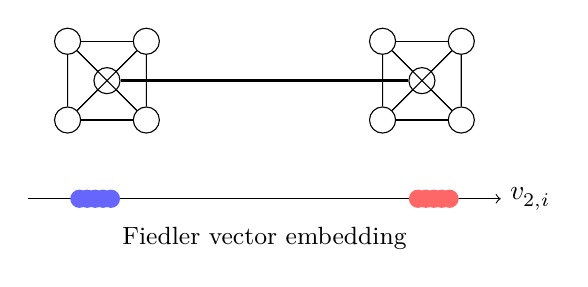
\begin{tikzpicture}
  \node[circle,draw] (A) at (0,0) {};
  \node[circle,draw] (B) at (0,1) {};
  \node[circle,draw] (C) at (1,0) {};
  \node[circle,draw] (D) at (1,1) {};
  \node[circle,draw] (E) at (0.5,0.5) {};
  \node[circle,draw] (F) at (4,0) {};
  \node[circle,draw] (G) at (4,1) {};
  \node[circle,draw] (H) at (5,0) {};
  \node[circle,draw] (I) at (5,1) {};
  \node[circle,draw] (J) at (4.5,0.5) {};
  \draw (A)--(B)--(C)--(D)--(A); \draw (A)--(C); \draw (B)--(D);
  \draw (A)--(E)--(B); \draw (C)--(E)--(D);
  \draw (F)--(G)--(H)--(I)--(F); \draw (F)--(H); \draw (G)--(I);
  \draw (F)--(J)--(G); \draw (H)--(J)--(I);
  \draw[very thick] (E) -- (J);
  \draw[->] (-0.5,-1) -- (5.5,-1) node[right] {$v_{2,i}$};
  \foreach \x in {0.15,0.25,0.35,0.45,0.55}
    \node[circle,fill=blue!60,scale=0.7] at (\x,-1) {};
  \foreach \x in {4.45,4.55,4.65,4.75,4.85}
    \node[circle,fill=red!60,scale=0.7] at (\x,-1) {};
  \node at (2.5,-1.5) {\small Fiedler vector embedding};
\end{tikzpicture}

The Fiedler value \(\lambda_2\) is very small (the bridge edge is a
bottleneck), and the Fiedler vector takes approximately \(-1/\sqrt{5}\)
on the left clique and \(+1/\sqrt{5}\) on the right, cleanly exposing
the natural partition.

\end{tcolorbox}

\begin{tcolorbox}[enhanced jigsaw, arc=.35mm, bottomrule=.15mm, bottomtitle=1mm, breakable, colback=white, colbacktitle=quarto-callout-warning-color!10!white, colframe=quarto-callout-warning-color-frame, coltitle=black, left=2mm, leftrule=.75mm, opacityback=0, opacitybacktitle=0.6, rightrule=.15mm, title={Exercise}, titlerule=0mm, toprule=.15mm, toptitle=1mm]

\textbf{(Spectral clustering on circles)} Generate \(n = 200\) points
sampled from two concentric circles using
\texttt{sklearn.datasets.make\textbackslash{}\_circles(n\textbackslash{}\_samples=200,\ noise=0.05,\ factor=0.4)}.

\begin{enumerate}
\def\labelenumi{\arabic{enumi}.}
\item
  Apply standard \(k\)-means (\(k=2\)) directly to the 2D coordinates.
  Does it succeed?
\item
  Construct a Gaussian similarity graph:
  \(w_{ij} = \exp(-\|x_i - x_j\|^2/(2\sigma^2))\) for \(\sigma = 0.3\);
  zero out edges with \(\|x_i - x_j\| > 3\sigma\).
\item
  Build \(\mathbf{L}_{\mathrm{sym}}\), compute its two smallest
  eigenvectors, and run \(k\)-means on the rows of \([\bv_1, \bv_2]\).
  Compare to the direct \(k\)-means result.
\item
  Plot \(\lambda_2\) vs.~\(\sigma \in \{0.1, 0.2, 0.3, 0.5, 1.0\}\).
  Which \(\sigma\) gives the best-separated clusters?
\end{enumerate}

\end{tcolorbox}

\section{Random Walks and Spectral
Gap}\label{random-walks-and-spectral-gap}

The matrix \(\bP = \bD^{-1}\bA\) defines the transition probabilities
for a simple random walk on the graph: from vertex \(i\), move to
neighbor \(j\) with probability \(w_{ij}/d_i\). This is a Markov chain
(see \Sabove for the full theory), and the spectral properties of the
Laplacian directly control its mixing behavior.

\begin{tcolorbox}[enhanced jigsaw, arc=.35mm, bottomrule=.15mm, bottomtitle=1mm, breakable, colback=white, colbacktitle=quarto-callout-note-color!10!white, colframe=quarto-callout-note-color-frame, coltitle=black, left=2mm, leftrule=.75mm, opacityback=0, opacitybacktitle=0.6, rightrule=.15mm, title={Definition: Random Walk on a Graph}, titlerule=0mm, toprule=.15mm, toptitle=1mm]

The \emph{simple random walk} on \(G\) is the Markov chain with
column-stochastic transition matrix
\[\bP = \bD^{-1}\bA, \qquad P_{ij} = \frac{w_{ij}}{d_j} \quad \text{if } (i,j)\in E, \quad 0 \text{ otherwise}.\]
The matrix \(\bP\) is related to the random-walk Laplacian by
\(\mathbf{L}_{\mathrm{rw}} = \bI - \bP\).

\end{tcolorbox}

\begin{tcolorbox}[enhanced jigsaw, arc=.35mm, bottomrule=.15mm, bottomtitle=1mm, breakable, colback=white, colbacktitle=quarto-callout-tip-color!10!white, colframe=quarto-callout-tip-color-frame, coltitle=black, left=2mm, leftrule=.75mm, opacityback=0, opacitybacktitle=0.6, rightrule=.15mm, title={Tip}, titlerule=0mm, toprule=.15mm, toptitle=1mm]

For a connected, non-bipartite graph, the random walk chain is
irreducible and aperiodic (ergodic in the sense of the result above). By
the Perron-Frobenius theorem (the result above), it has a unique
stationary distribution. For the simple random walk, detailed balance
holds with \(\boldsymbol{\pi} = \boldsymbol{d}/\|\boldsymbol{d}\|_1\)
where \(\boldsymbol{d} = (d_1,...,d_n)^T\): in this sense the walk is
reversible. For a \(d\)-regular graph,
\(\boldsymbol{\pi} = \mathbf{1}/n\) (uniform distribution). The spectral
gap of \(\bP\) equals the Fiedler value
\(\lambda_2(\mathbf{L}_{\mathrm{rw}})\), so the mixing time
\(k_\varepsilon \approx \log(n)/\lambda_2\) is determined entirely by
the graph's spectral connectivity.

\end{tcolorbox}

\begin{tcolorbox}[enhanced jigsaw, arc=.35mm, bottomrule=.15mm, bottomtitle=1mm, breakable, colback=white, colbacktitle=quarto-callout-warning-color!10!white, colframe=quarto-callout-warning-color-frame, coltitle=black, left=2mm, leftrule=.75mm, opacityback=0, opacitybacktitle=0.6, rightrule=.15mm, title={Exercise}, titlerule=0mm, toprule=.15mm, toptitle=1mm]

\textbf{(Random walk mixing on graphs)} For the path \(P_{10}\), cycle
\(C_{10}\), and complete graph \(K_{10}\):

\begin{enumerate}
\def\labelenumi{\arabic{enumi}.}
\item
  Build \(\bP = \bD^{-1}\bA\) and compute the spectral gap
  \(\delta = 1 - |\lambda_2(\bP)|\) for each.
\item
  Simulate the random walk for 200 steps from \(\bx^{(0)} = \be_1\).
  Plot \(\|\bx^{(k)} - \boldsymbol{\pi}\|_1\) vs.~\(k\) on a semi-log
  scale.
\item
  The theoretical mixing time is
  \(k_\varepsilon \approx \log(n)/\delta\) for \(\varepsilon = 0.01\).
  How does the empirical mixing time compare across the three graphs?
\end{enumerate}

\end{tcolorbox}

\section{PageRank}\label{pagerank}

PageRank, developed by Brin and Page at Google, measures the importance
of web pages by modeling a random surfer navigating the web graph. Its
mathematical foundation is the Perron-Frobenius theorem applied to a
specially constructed column-stochastic matrix. The algorithm reduces to
power iteration on the random walk chain, connecting web search to the
spectral graph theory developed in this section.

\begin{tcolorbox}[enhanced jigsaw, arc=.35mm, bottomrule=.15mm, bottomtitle=1mm, breakable, colback=white, colbacktitle=quarto-callout-note-color!10!white, colframe=quarto-callout-note-color-frame, coltitle=black, left=2mm, leftrule=.75mm, opacityback=0, opacitybacktitle=0.6, rightrule=.15mm, title={Definition: Web Graph and Random Surfer}, titlerule=0mm, toprule=.15mm, toptitle=1mm]

The web is modeled as a directed graph \(G = (V,E)\) where \(V\) is the
set of \(N\) pages and \((p_j, p_i) \in E\) if page \(p_j\) links to
page \(p_i\). Let \(L(p_j)\) denote the number of outbound links from
\(p_j\). The \emph{random surfer} navigates by: at each step, clicking a
uniformly random outbound link from the current page (or, if the current
page has no outbound links, jumping uniformly to any page).

\end{tcolorbox}

\begin{tcolorbox}[enhanced jigsaw, arc=.35mm, bottomrule=.15mm, bottomtitle=1mm, breakable, colback=white, colbacktitle=quarto-callout-warning-color!10!white, colframe=quarto-callout-warning-color-frame, coltitle=black, left=2mm, leftrule=.75mm, opacityback=0, opacitybacktitle=0.6, rightrule=.15mm, title={Exercise}, titlerule=0mm, toprule=.15mm, toptitle=1mm]

\textbf{(Web graph modeling)} For the 4-page web graph with edges
\(P_1 \to P_2\), \(P_1 \to P_3\), \(P_2 \to P_4\), \(P_3 \to P_2\),
\(P_3 \to P_4\), \(P_4 \to P_1\):

\begin{enumerate}
\def\labelenumi{\arabic{enumi}.}
\item
  Draw the directed graph. Which pages are most-linked-to?
\item
  Identify any dangling nodes (pages with \(L(p_j) = 0\)). What should
  the random surfer do at a dangling node?
\item
  Without any computation, rank the four pages by expected importance
  based on the graph structure. Record your guess to compare against the
  computed PageRank.
\end{enumerate}

\end{tcolorbox}

\begin{tcolorbox}[enhanced jigsaw, arc=.35mm, bottomrule=.15mm, bottomtitle=1mm, breakable, colback=white, colbacktitle=quarto-callout-note-color!10!white, colframe=quarto-callout-note-color-frame, coltitle=black, left=2mm, leftrule=.75mm, opacityback=0, opacitybacktitle=0.6, rightrule=.15mm, title={Definition: Hyperlink and Stochastic Matrices}, titlerule=0mm, toprule=.15mm, toptitle=1mm]

Define the \emph{hyperlink matrix} \(\bH \in \fR^{N\times N}\) by
\(H_{ij} = 1/L(p_j)\) if \(p_j\) links to \(p_i\) and \(L(p_j) > 0\),
zero otherwise. Since columns for dangling nodes (where \(L(p_j) = 0\))
sum to zero, \(\bH\) is not stochastic. The \emph{stochastic matrix}
\(\bS\) fixes this:
\[S_{ij} = \begin{cases} 1/L(p_j) & \text{if } (p_j, p_i) \in E \text{ and } L(p_j) > 0, \\ 1/N & \text{if } L(p_j) = 0 \text{ (dangling node column)}, \\ 0 & \text{otherwise.}\end{cases}\]
Every column of \(\bS\) sums to 1, so \(\bS\) is column-stochastic.

\end{tcolorbox}

\begin{tcolorbox}[enhanced jigsaw, arc=.35mm, bottomrule=.15mm, bottomtitle=1mm, breakable, colback=white, colbacktitle=quarto-callout-tip-color!10!white, colframe=quarto-callout-tip-color-frame, coltitle=black, left=2mm, leftrule=.75mm, opacityback=0, opacitybacktitle=0.6, rightrule=.15mm, title={Tip}, titlerule=0mm, toprule=.15mm, toptitle=1mm]

The basic PageRank equation \(\mathbf{r} = \bS\mathbf{r}\) requires
\(\bS\) to be irreducible and primitive to guarantee a unique stationary
distribution. However, \(\bS\) can fail both conditions: a set of pages
that link only among themselves (a \emph{rank sink}) can trap the
surfer. Even with dangling node corrections, \(\bS\) may have multiple
eigenvalues equal to 1, making the stationary distribution non-unique
and power iteration non-convergent.

\end{tcolorbox}

\begin{tcolorbox}[enhanced jigsaw, arc=.35mm, bottomrule=.15mm, bottomtitle=1mm, breakable, colback=white, colbacktitle=quarto-callout-note-color!10!white, colframe=quarto-callout-note-color-frame, coltitle=black, left=2mm, leftrule=.75mm, opacityback=0, opacitybacktitle=0.6, rightrule=.15mm, title={Theorem: Perron-Frobenius Theorem}, titlerule=0mm, toprule=.15mm, toptitle=1mm]

Let \(\mathbf{G} \in \fR^{n\times n}\) be a matrix with all positive
entries (\(G_{ij} > 0\)). Then:

\begin{enumerate}
\def\labelenumi{\arabic{enumi}.}
\item
  \(\mathbf{G}\) has a unique largest eigenvalue \(\rho > 0\) (the
  \emph{Perron root}) with \(\rho > |\lambda_j|\) for all other
  eigenvalues \(\lambda_j\).
\item
  The corresponding eigenvector \(\bv_1\) (the \emph{Perron vector}) has
  all strictly positive entries and is unique up to scaling.
\item
  \(\rho\) is a simple eigenvalue.
\end{enumerate}

If \(\mathbf{G}\) is nonnegative, irreducible, and primitive, the same
three conclusions hold.

\end{tcolorbox}

\begin{tcolorbox}[enhanced jigsaw, arc=.35mm, bottomrule=.15mm, bottomtitle=1mm, breakable, colback=white, colbacktitle=quarto-callout-tip-color!10!white, colframe=quarto-callout-tip-color-frame, coltitle=black, left=2mm, leftrule=.75mm, opacityback=0, opacitybacktitle=0.6, rightrule=.15mm, title={Proof}, titlerule=0mm, toprule=.15mm, toptitle=1mm]

\textbf{Step 1: Existence via Brouwer.} Define the simplex
\(\Delta = \{\bx \geq \bzero : \|\bx\|_1 = 1\}\) and the normalized map
\(T(\bx) = \mathbf{G}\bx/\|\mathbf{G}\bx\|_1\). Since
\(\mathbf{G} > 0\), \(T\) maps \(\Delta\) into its interior and is
continuous, so Brouwer's fixed-point theorem gives a \(\bv > 0\) with
\(T(\bv) = \bv\), i.e., \(\mathbf{G}\bv = \rho\bv\) for
\(\rho = \|\mathbf{G}\bv\|_1 > 0\).

\textbf{Step 2: Dominance \(\rho > |\lambda_j|\).} For any eigenvalue
\(\lambda\) with eigenvector \(\bw\), let \(i^*\) maximize
\(|w_{i^*}| = \|\bw\|_\infty\). Then
\(|\lambda||w_{i^*}| = |(\mathbf{G}\bw)_{i^*}| \leq \sum_j G_{i^*j}|w_j| < |w_{i^*}|\sum_j G_{i^*j} \leq |w_{i^*}|\rho\)
(using \(G > 0\) and \$\rho = \$ spectral radius). This gives
\(|\lambda| < \rho\) strictly (since all \(G_{ij} > 0\) prevents
equality in the second step unless \(\bw\) is a multiple of \(\bv\)).

\textbf{Step 3: Uniqueness and simplicity.} Since \(\rho\) is strictly
larger than all other eigenvalues in magnitude, its eigenspace is
one-dimensional and \(\rho\) is algebraically simple.

\end{tcolorbox}

\begin{tcolorbox}[enhanced jigsaw, arc=.35mm, bottomrule=.15mm, bottomtitle=1mm, breakable, colback=white, colbacktitle=quarto-callout-note-color!10!white, colframe=quarto-callout-note-color-frame, coltitle=black, left=2mm, leftrule=.75mm, opacityback=0, opacitybacktitle=0.6, rightrule=.15mm, title={Definition: Google Matrix}, titlerule=0mm, toprule=.15mm, toptitle=1mm]

The \emph{Google matrix} introduces a \emph{damping factor}
\(d \in (0,1)\) (typically \(d = 0.85\)): with probability \(d\) the
surfer follows a random link, and with probability \(1-d\) the surfer
teleports to a uniformly random page. This gives
\[\mathbf{G} = d\,\bS + \frac{1-d}{N}\,\mathbf{J},\] where
\(\mathbf{J} = \mathbf{1}\mathbf{1}^T\) is the \(N\times N\) all-ones
matrix. The PageRank vector \(\mathbf{r}\) is the unique stationary
distribution of \(\mathbf{G}\): \(\mathbf{G}\mathbf{r} = \mathbf{r}\).

\end{tcolorbox}

\begin{tcolorbox}[enhanced jigsaw, arc=.35mm, bottomrule=.15mm, bottomtitle=1mm, breakable, colback=white, colbacktitle=quarto-callout-note-color!10!white, colframe=quarto-callout-note-color-frame, coltitle=black, left=2mm, leftrule=.75mm, opacityback=0, opacitybacktitle=0.6, rightrule=.15mm, title={Theorem: PageRank Is Well-Posed}, titlerule=0mm, toprule=.15mm, toptitle=1mm]

The Google matrix \(\mathbf{G} = d\bS + \frac{1-d}{N}\mathbf{J}\) is
column-stochastic, irreducible, and primitive for any \(d \in (0,1)\)
and any \(\bS\). By the Perron-Frobenius theorem (the result above),
\(\mathbf{G}\) has a unique positive stationary distribution
\(\mathbf{r}\) with \(\sum_i r_i = 1\).

\end{tcolorbox}

\begin{tcolorbox}[enhanced jigsaw, arc=.35mm, bottomrule=.15mm, bottomtitle=1mm, breakable, colback=white, colbacktitle=quarto-callout-tip-color!10!white, colframe=quarto-callout-tip-color-frame, coltitle=black, left=2mm, leftrule=.75mm, opacityback=0, opacitybacktitle=0.6, rightrule=.15mm, title={Proof}, titlerule=0mm, toprule=.15mm, toptitle=1mm]

\textbf{Step 1: Column-stochastic.} Since \(\bS\) is column-stochastic
and \(\frac{1}{N}\mathbf{J}\) has all columns equal to
\(\frac{1}{N}\mathbf{1}\) (which sums to 1), the convex combination
\(\mathbf{G} = d\bS + (1-d)\frac{\mathbf{J}}{N}\) is also
column-stochastic.

\textbf{Step 2: All entries positive.} The term
\(\frac{1-d}{N}\mathbf{J}\) has all entries equal to
\(\frac{1-d}{N} > 0\) (since \(d < 1\)). Adding any nonnegative matrix
\(d\bS \geq 0\) preserves positivity, so all entries of \(\mathbf{G}\)
are at least \(\frac{1-d}{N} > 0\).

\textbf{Step 3: Perron-Frobenius applies.} Since \(\mathbf{G}\) has all
positive entries, the result above applies: the Perron root is
\(\rho = 1\) (column-stochastic implies
\(\mathbf{1}^T\mathbf{G} = \mathbf{1}^T\), so \(\rho = 1\)), it is
simple, and the Perron vector \(\mathbf{r} > 0\) is unique up to
scaling. Normalizing to \(\|\mathbf{r}\|_1 = 1\) gives the unique
PageRank vector.

\end{tcolorbox}

\begin{tcolorbox}[enhanced jigsaw, arc=.35mm, bottomrule=.15mm, bottomtitle=1mm, breakable, colback=white, colbacktitle=quarto-callout-tip-color!10!white, colframe=quarto-callout-tip-color-frame, coltitle=black, left=2mm, leftrule=.75mm, opacityback=0, opacitybacktitle=0.6, rightrule=.15mm, title={Tip}, titlerule=0mm, toprule=.15mm, toptitle=1mm]

The PageRank power iteration
\(\mathbf{r}^{(k+1)} = \mathbf{G}\mathbf{r}^{(k)}\) does not require
forming \(\mathbf{G}\) explicitly (which is dense). Using
\(\mathbf{J}\mathbf{r}^{(k)} = \mathbf{1}\) (since
\(\|\mathbf{r}^{(k)}\|_1 = 1\)):
\[\mathbf{r}^{(k+1)} = d\,\bS\mathbf{r}^{(k)} + \frac{1-d}{N}\mathbf{1}.\]
Only the sparse \(\bS\) multiply is needed. The convergence rate is
\(d\cdot|\lambda_2(\bS)|\), and since all eigenvalues of \(\mathbf{G}\)
beyond the first satisfy \(|\lambda_i(\mathbf{G})| \leq d\), the
spectral gap is at least \(1 - d = 0.15\) for \(d = 0.85\). With
\(n \sim 10^9\) pages, about 130 iterations suffice.

\end{tcolorbox}

\begin{tcolorbox}[enhanced jigsaw, arc=.35mm, bottomrule=.15mm, bottomtitle=1mm, breakable, colback=white, colbacktitle=quarto-callout-warning-color!10!white, colframe=quarto-callout-warning-color-frame, coltitle=black, left=2mm, leftrule=.75mm, opacityback=0, opacitybacktitle=0.6, rightrule=.15mm, title={Exercise}, titlerule=0mm, toprule=.15mm, toptitle=1mm]

\textbf{(PageRank by hand and by power iteration)} For the 4-page web
graph from the first exercise in this subsubsection:

\begin{enumerate}
\def\labelenumi{\arabic{enumi}.}
\item
  Construct \(\bS\) (column-stochastic). Are there dangling nodes?
\item
  Set \(d = 0.85\) and build \(\mathbf{G}\). Verify all columns sum to 1
  and all entries are positive.
\item
  Run 10 steps of
  \(\mathbf{r}^{(k+1)} = d\bS\mathbf{r}^{(k)} + \frac{1-d}{N}\mathbf{1}\)
  from \(\mathbf{r}^{(0)} = \frac{1}{4}\mathbf{1}\). Report
  \(\mathbf{r}^{(k)}\) at steps 1, 5, and 10.
\item
  Solve for the exact \(\mathbf{r}\) using \texttt{numpy.linalg.eig(G)}
  and compare to your power iteration result. Which page is most
  important? Does it match your initial guess?
\end{enumerate}

\end{tcolorbox}

\begin{tcolorbox}[enhanced jigsaw, arc=.35mm, bottomrule=.15mm, bottomtitle=1mm, breakable, colback=white, colbacktitle=quarto-callout-warning-color!10!white, colframe=quarto-callout-warning-color-frame, coltitle=black, left=2mm, leftrule=.75mm, opacityback=0, opacitybacktitle=0.6, rightrule=.15mm, title={Exercise}, titlerule=0mm, toprule=.15mm, toptitle=1mm]

\textbf{(Convergence rate and damping factor)} For the 4-page graph
above:

\begin{enumerate}
\def\labelenumi{\arabic{enumi}.}
\item
  Compute all eigenvalues of \(\mathbf{G}\) for \(d = 0.85\). What is
  the spectral gap \(1 - |\lambda_2(\mathbf{G})|\)?
\item
  Repeat for \(d \in \{0.5, 0.7, 0.85, 0.95\}\). Plot the spectral gap
  vs.~\(d\). For which \(d\) does power iteration converge fastest?
\item
  For a disconnected graph with two components (no cross-links), \(\bS\)
  has eigenvalue 1 with multiplicity 2. Explain why the teleportation
  term \(\frac{1-d}{N}\mathbf{J}\) is essential: what happens to the
  second eigenvalue of \(\mathbf{G}\) as \(d \to 1\)?
\end{enumerate}

\end{tcolorbox}

\begin{tcolorbox}[enhanced jigsaw, arc=.35mm, bottomrule=.15mm, bottomtitle=1mm, breakable, colback=white, colbacktitle=quarto-callout-warning-color!10!white, colframe=quarto-callout-warning-color-frame, coltitle=black, left=2mm, leftrule=.75mm, opacityback=0, opacitybacktitle=0.6, rightrule=.15mm, title={Exercise}, titlerule=0mm, toprule=.15mm, toptitle=1mm]

\textbf{(Large-scale PageRank implementation)} Implement the efficient
PageRank iteration using sparse matrices:

\begin{enumerate}
\def\labelenumi{\arabic{enumi}.}
\item
  Generate a random directed graph on \(N = 1000\) nodes using
  \texttt{networkx.gnm\textbackslash{}\_random\textbackslash{}\_graph(1000,\ 5000,\ directed=True)}.
  Identify and handle dangling nodes.
\item
  Store \(\bS\) as a SciPy CSR sparse matrix. Implement the iteration
  \(\mathbf{r}^{(k+1)} = d\bS\mathbf{r}^{(k)} + \frac{1-d}{N}\mathbf{1}\)
  and run until
  \(\|\mathbf{r}^{(k+1)} - \mathbf{r}^{(k)}\|_1 < 10^{-8}\).
\item
  Plot the \(\ell^1\) convergence gap vs.~iteration on a semi-log scale.
  Measure the empirical convergence rate and compare to the theoretical
  bound \(d = 0.85\).
\item
  Report the top-10 pages by PageRank. How does the ranking change when
  \(d\) is varied from 0.5 to 0.95?
\end{enumerate}

\end{tcolorbox}

\chapter{Linear Operators and the Poisson
Equation}\label{linear-operators-and-the-poisson-equation}

This subsection is a supplement to Lab 4, which asks you to solve the
Poisson heat equation numerically. The lab will have you build a large
sparse matrix and solve a linear system with it. Before doing that, it
is worth understanding where that matrix comes from and why it has the
properties it does. We will see that it is a finite-dimensional
approximation of a differential operator, and that studying its
eigenvalues gives insight into both the physics of the problem and the
difficulty of solving it numerically. Spectral theory, which you have
already seen for matrices, extends to this setting in a way that is both
natural and surprising.

\section{From Differential Operators to
Matrices}\label{from-differential-operators-to-matrices}

\begin{tcolorbox}[enhanced jigsaw, arc=.35mm, bottomrule=.15mm, bottomtitle=1mm, breakable, colback=white, colbacktitle=quarto-callout-note-color!10!white, colframe=quarto-callout-note-color-frame, coltitle=black, left=2mm, leftrule=.75mm, opacityback=0, opacitybacktitle=0.6, rightrule=.15mm, title={Definition: Linear Operator}, titlerule=0mm, toprule=.15mm, toptitle=1mm]

Let \(X\) and \(Y\) be vector spaces of functions. A map
\(\mathcal{A} : X \to Y\) is a \emph{linear operator} if for all
\(u, v \in X\) and scalars \(\alpha\):
\[\mathcal{A}(\alpha u + v) = \alpha\,\mathcal{A}u + \mathcal{A}v.\]
Every matrix \(\bA \in \fR^{m \times n}\) is a linear operator from
\(\fR^n\) to \(\fR^m\). Differential operators such as \(\frac{d}{dx}\)
and \(\nabla^2\) are linear operators on function spaces (e.g., on the
space of twice-differentiable functions on \([0,1]\)).

\end{tcolorbox}

The central idea of numerical methods for PDEs is \emph{discretization}:
replace an infinite-dimensional operator by a finite matrix that
approximates it on a grid. The accuracy of the approximation improves as
the grid is refined (grid spacing \(h \to 0\)), and the resulting
matrices get larger (\(n \to \infty\)). Everything in Lab 4 is an
instance of this: the \(n^2 \times n^2\) matrix you will assemble is the
\(n\)-point discretization of the continuous Laplacian \(-\nabla^2\).

\begin{tcolorbox}[enhanced jigsaw, arc=.35mm, bottomrule=.15mm, bottomtitle=1mm, breakable, colback=white, colbacktitle=quarto-callout-note-color!10!white, colframe=quarto-callout-note-color-frame, coltitle=black, left=2mm, leftrule=.75mm, opacityback=0, opacitybacktitle=0.6, rightrule=.15mm, title={Definition: Finite Difference Approximation}, titlerule=0mm, toprule=.15mm, toptitle=1mm]

The \emph{centered second-difference} approximation to \(u''(x)\) at a
grid point \(x_k\) with spacing \(h\) is
\[u''(x_k) \approx \frac{u(x_{k-1}) - 2u(x_k) + u(x_{k+1})}{h^2}.\] To
see why, expand \(u\) at \(x_k \pm h\) via Taylor series:
\[u(x_k + h) = u(x_k) + h u'(x_k) + \tfrac{h^2}{2}u''(x_k) + \tfrac{h^3}{6}u'''(x_k) + O(h^4),\]
\[u(x_k - h) = u(x_k) - h u'(x_k) + \tfrac{h^2}{2}u''(x_k) - \tfrac{h^3}{6}u'''(x_k) + O(h^4).\]
Adding these two equations cancels the odd-order terms, leaving
\[u(x_k + h) + u(x_k - h) = 2u(x_k) + h^2 u''(x_k) + O(h^4).\]
Rearranging gives the formula above, with error \(O(h^2)\). This is
called \emph{second-order accuracy}: halving \(h\) reduces the error by
a factor of four.

\end{tcolorbox}

\section{The Discrete Laplacian}\label{the-discrete-laplacian}

\begin{tcolorbox}[enhanced jigsaw, arc=.35mm, bottomrule=.15mm, bottomtitle=1mm, breakable, colback=white, colbacktitle=quarto-callout-note-color!10!white, colframe=quarto-callout-note-color-frame, coltitle=black, left=2mm, leftrule=.75mm, opacityback=0, opacitybacktitle=0.6, rightrule=.15mm, title={Definition: 1-D Discrete Laplacian}, titlerule=0mm, toprule=.15mm, toptitle=1mm]

On \([0,1]\) with \(n\) interior grid points \(x_k = kh\),
\(h = 1/(n+1)\), and homogeneous Dirichlet boundary conditions
\(u(0) = u(1) = 0\), the operator \(-d^2/dx^2\) is discretized by
applying the finite difference formula at each interior point. The
result is the tridiagonal linear system \(\bT\mathbf{u} = \mathbf{f}\),
where \[\bT = \frac{1}{h^2}
  \begin{pmatrix}
    2  & -1 &        &        \\
    -1 &  2 & -1     &        \\
       & \ddots & \ddots & \ddots \\
       &        & -1     & 2
  \end{pmatrix}
  \in \fR^{n \times n}.\] The \(-1\) off-diagonals come from the
neighbor terms \(u(x_{k\pm1})\); the \(2\) on the diagonal comes from
\(-2u(x_k)\); and the \(1/h^2\) scaling comes from the approximation
formula. The boundary values \(u(0) = u(1) = 0\) are incorporated by
simply omitting them from the system.

\end{tcolorbox}

\begin{tcolorbox}[enhanced jigsaw, arc=.35mm, bottomrule=.15mm, bottomtitle=1mm, breakable, colback=white, colbacktitle=quarto-callout-note-color!10!white, colframe=quarto-callout-note-color-frame, coltitle=black, left=2mm, leftrule=.75mm, opacityback=0, opacitybacktitle=0.6, rightrule=.15mm, title={Theorem: Eigenvalues of the 1-D Discrete Laplacian}, titlerule=0mm, toprule=.15mm, toptitle=1mm]

The matrix \(\bT \in \fR^{n \times n}\) has eigenvalues
\[\lambda_k = \frac{4}{h^2}\sin^2\!\left(\frac{k\pi}{2(n+1)}\right), \quad k = 1, ..., n,\]
with corresponding eigenvectors \((\bv_k)_j = \sin(jk\pi h)\),
\(j = 1, ..., n\). As \(n \to \infty\), these eigenvalues satisfy
\(\lambda_k \to k^2\pi^2\), which are exactly the eigenvalues of the
continuous operator \(-d^2/dx^2\) on \([0,1]\).

\end{tcolorbox}

\begin{tcolorbox}[enhanced jigsaw, arc=.35mm, bottomrule=.15mm, bottomtitle=1mm, breakable, colback=white, colbacktitle=quarto-callout-tip-color!10!white, colframe=quarto-callout-tip-color-frame, coltitle=black, left=2mm, leftrule=.75mm, opacityback=0, opacitybacktitle=0.6, rightrule=.15mm, title={Proof}, titlerule=0mm, toprule=.15mm, toptitle=1mm]

We verify by direct substitution that \(\bT\bv_k = \lambda_k \bv_k\).

\textbf{Step 1: Compute the \(j\)-th entry of \(\bT\bv_k\).}

The tridiagonal structure gives
\[(\bT\bv_k)_j = \frac{1}{h^2}\bigl(-\sin((j-1)k\pi h) + 2\sin(jk\pi h) - \sin((j+1)k\pi h)\bigr).\]

\textbf{Step 2: Apply a trigonometric identity.}

Using the sum-to-product identity
\(-\sin(\theta - \phi) + 2\sin\theta - \sin(\theta + \phi) = 2\sin\theta(1 - \cos\phi)\)
with \(\theta = jk\pi h\) and \(\phi = k\pi h\), the expression becomes
\[(\bT\bv_k)_j = \frac{2(1 - \cos(k\pi h))}{h^2}\sin(jk\pi h).\]

\textbf{Step 3: Simplify using the half-angle identity.}

Since \(1 - \cos\phi = 2\sin^2(\phi/2)\), we get
\[(\bT\bv_k)_j = \frac{4}{h^2}\sin^2\!\left(\frac{k\pi h}{2}\right) \cdot (\bv_k)_j = \lambda_k\,(\bv_k)_j.\]
This confirms \(\bv_k\) is an eigenvector with eigenvalue \(\lambda_k\).

\textbf{Step 4: The continuous limit.}

As \(h \to 0\), use \(\sin(\theta) \approx \theta\) for small
\(\theta\):
\[\lambda_k = \frac{4}{h^2}\sin^2\!\left(\frac{k\pi h}{2}\right)
  \approx \frac{4}{h^2} \cdot \frac{k^2\pi^2 h^2}{4} = k^2\pi^2.\] The
discrete eigenvalues converge to the continuous eigenvalues
\(k^2\pi^2\).

\end{tcolorbox}

\begin{tcolorbox}[enhanced jigsaw, arc=.35mm, bottomrule=.15mm, bottomtitle=1mm, breakable, colback=white, colbacktitle=quarto-callout-note-color!10!white, colframe=quarto-callout-note-color-frame, coltitle=black, left=2mm, leftrule=.75mm, opacityback=0, opacitybacktitle=0.6, rightrule=.15mm, title={Definition: 2-D Discrete Laplacian (Poisson Equation)}, titlerule=0mm, toprule=.15mm, toptitle=1mm]

On the unit square \([0,1]^2\) with an \(n \times n\) interior grid
(\(N = n^2\) unknowns), the five-point finite difference stencil
approximates \(-\nabla^2 u = f\) at each grid point \((x_i, y_j)\) as
\[\frac{1}{h^2}\bigl(4u_{ij} - u_{i+1,j} - u_{i-1,j} - u_{i,j+1} - u_{i,j-1}\bigr) = f_{ij}.\]
After flattening the 2-D grid to a 1-D index \(k = j + n \cdot i\), this
becomes the block tridiagonal system
\(\mathbf{K}\mathbf{u} = \mathbf{f}\) where \[\mathbf{K} = \frac{1}{h^2}
  \begin{pmatrix}
    \mathbf{C} & -\bI       &            &            \\
    -\bI       & \mathbf{C} & -\bI       &            \\
               & \ddots     & \ddots     & \ddots     \\
               &            & -\bI       & \mathbf{C}
  \end{pmatrix},
  \qquad
  \mathbf{C} = \mathrm{tridiag}(-1,\, 4,\, -1) \in \fR^{n \times n}.\]
Each diagonal block \(\mathbf{C}\) encodes the \(x\)-direction neighbors
of a row of grid points. The off-diagonal \(-\bI\) blocks connect rows
that are adjacent in \(y\), which appear \(n\) positions apart in the
flattened index.

\end{tcolorbox}

\begin{tcolorbox}[enhanced jigsaw, arc=.35mm, bottomrule=.15mm, bottomtitle=1mm, breakable, colback=white, colbacktitle=quarto-callout-tip-color!10!white, colframe=quarto-callout-tip-color-frame, coltitle=black, left=2mm, leftrule=.75mm, opacityback=0, opacitybacktitle=0.6, rightrule=.15mm, title={Tip}, titlerule=0mm, toprule=.15mm, toptitle=1mm]

The matrix \(\mathbf{K}\) is symmetric positive definite
(Section\textasciitilde above), so the Poisson system has a unique
solution. In practice, \(\mathbf{K}\) is extremely sparse (at most 5
nonzeros per row out of \(N = n^2\)), so it is stored and solved using
\texttt{scipy.sparse}, exactly as you will do in Lab 4. A direct sparse
solve costs \(O(N^{3/2})\) for 2-D problems, far better than the
\(O(N^3)\) dense cost.

\end{tcolorbox}

\begin{tcolorbox}[enhanced jigsaw, arc=.35mm, bottomrule=.15mm, bottomtitle=1mm, breakable, colback=white, colbacktitle=quarto-callout-warning-color!10!white, colframe=quarto-callout-warning-color-frame, coltitle=black, left=2mm, leftrule=.75mm, opacityback=0, opacitybacktitle=0.6, rightrule=.15mm, title={Exercise}, titlerule=0mm, toprule=.15mm, toptitle=1mm]

\begin{enumerate}
\def\labelenumi{\arabic{enumi}.}
\item
  Using \texttt{scipy.sparse.diags}, build the 1-D discrete Laplacian
  \(\bT\) for \(n = 50\) interior points. Compute its eigenvalues with
  \texttt{np.linalg.eigvalsh} and compare them to the analytical formula
  \(\lambda_k = \frac{4}{h^2}\sin^2(k\pi h/2)\) for \(k = 1, ..., 50\).
  Plot both sets on the same axes.
\item
  Verify that the eigenvectors satisfy \((\bv_k)_j = \sin(jk\pi h)\) by
  calling \texttt{np.linalg.eigh(T.toarray())} and plotting the first
  three eigenvectors. Do they look like \(\sin(k\pi x)\)?
\item
  Extend the Lab 4 code to impose a non-homogeneous Dirichlet boundary
  condition \(u = g\) on the boundary of \([0,1]^2\) by modifying the
  right-hand side \(\mathbf{f}\).
  (\textit{Hint: for each boundary node $k$, replace row $k$ of $\mathbf{K}$ with
    the corresponding identity row and set $f_k = g(x_k)$.})
\end{enumerate}

\end{tcolorbox}

\section{Operator Norms and
Boundedness}\label{operator-norms-and-boundedness}

For matrices, the operator norm \(\|\bA\|_2 = \sigma_{\max}(\bA)\) is
always finite. The same is not true for differential operators on
function spaces. The distinction between \emph{bounded} and
\emph{unbounded} operators is one of the fundamental differences between
finite and infinite dimensions, and it has direct consequences for the
numerical conditioning of PDE-based linear systems.

\begin{tcolorbox}[enhanced jigsaw, arc=.35mm, bottomrule=.15mm, bottomtitle=1mm, breakable, colback=white, colbacktitle=quarto-callout-note-color!10!white, colframe=quarto-callout-note-color-frame, coltitle=black, left=2mm, leftrule=.75mm, opacityback=0, opacitybacktitle=0.6, rightrule=.15mm, title={Definition: Bounded Linear Operator}, titlerule=0mm, toprule=.15mm, toptitle=1mm]

A linear operator \(\mathcal{A} : X \to Y\) between normed function
spaces is \emph{bounded} if there exists a constant \(C < \infty\) such
that
\[\|\mathcal{A}u\|_Y \leq C\,\|u\|_X \quad \text{for all } u \in X.\]
The \emph{operator norm} is defined analogously to the matrix case:
\[\|\mathcal{A}\|_{\mathrm{op}} = \sup_{\|u\|_X = 1} \|\mathcal{A}u\|_Y.\]
Every matrix \(\bA \in \fR^{m \times n}\) is a bounded operator with
\(\|\bA\|_{\mathrm{op}} = \|\bA\|_2 = \sigma_{\max}(\bA)\).

\end{tcolorbox}

\begin{tcolorbox}[enhanced jigsaw, arc=.35mm, bottomrule=.15mm, bottomtitle=1mm, breakable, colback=white, colbacktitle=quarto-callout-note-color!10!white, colframe=quarto-callout-note-color-frame, coltitle=black, left=2mm, leftrule=.75mm, opacityback=0, opacitybacktitle=0.6, rightrule=.15mm, title={Theorem: The Differentiation Operator is Unbounded}, titlerule=0mm, toprule=.15mm, toptitle=1mm]

The operator \(\mathcal{D} = -d^2/dx^2\) on \(L^2[0,1]\) with domain
\(\{u \in L^2[0,1] : u'' \in L^2,\; u(0)=u(1)=0\}\) is \emph{unbounded}:
no finite constant \(C\) satisfies \(\|\mathcal{D}u\|_2 \leq C\|u\|_2\)
for all \(u\) in its domain.

\end{tcolorbox}

\begin{tcolorbox}[enhanced jigsaw, arc=.35mm, bottomrule=.15mm, bottomtitle=1mm, breakable, colback=white, colbacktitle=quarto-callout-tip-color!10!white, colframe=quarto-callout-tip-color-frame, coltitle=black, left=2mm, leftrule=.75mm, opacityback=0, opacitybacktitle=0.6, rightrule=.15mm, title={Proof}, titlerule=0mm, toprule=.15mm, toptitle=1mm]

To show \(\mathcal{D}\) is unbounded, we exhibit a sequence of unit-norm
functions on which \(\|\mathcal{D}u_k\|_2\) grows without bound.

\textbf{Step 1: Define a sequence of test functions.}

Let \(u_k(x) = \sqrt{2}\sin(k\pi x)\) for \(k = 1, 2, 3, ...\). Each
\(u_k\) satisfies the boundary conditions \(u_k(0) = u_k(1) = 0\).

\textbf{Step 2: Verify each \(u_k\) has unit norm.}

\[\|u_k\|_2^2 = 2\int_0^1 \sin^2(k\pi x)\,dx = 2 \cdot \tfrac{1}{2} = 1.\]

\textbf{Step 3: Compute $\mathcal{D}u_k$.}

Differentiating twice:
\(-u_k''(x) = k^2\pi^2\sqrt{2}\sin(k\pi x) = k^2\pi^2\,u_k(x)\). So
\(u_k\) is actually an eigenfunction of \(\mathcal{D}\), and
\[\|\mathcal{D}u_k\|_2 = k^2\pi^2\|u_k\|_2 = k^2\pi^2.\]

\textbf{Step 4: Conclude.}

For any candidate bound \(C\), choose \(k > \sqrt{C}/\pi\). Then
\(k^2\pi^2 > C\), so \(\|\mathcal{D}u_k\|_2 > C = C\|u_k\|_2\). Since no
finite \(C\) works, \(\mathcal{D}\) is unbounded.

\end{tcolorbox}

\begin{tcolorbox}[enhanced jigsaw, arc=.35mm, bottomrule=.15mm, bottomtitle=1mm, breakable, colback=white, colbacktitle=quarto-callout-tip-color!10!white, colframe=quarto-callout-tip-color-frame, coltitle=black, left=2mm, leftrule=.75mm, opacityback=0, opacitybacktitle=0.6, rightrule=.15mm, title={Tip}, titlerule=0mm, toprule=.15mm, toptitle=1mm]

Although the continuous operator is unbounded, its \(n\)-point
discretization \(\bT\) has operator norm
\(\|\bT\|_2 = \lambda_{\max}(\bT) \approx 4/h^2 = 4(n+1)^2\), which is
large but finite. This growing norm explains why Poisson systems become
increasingly ill-conditioned as the grid is refined:
\[\kappa(\bT) = \frac{\lambda_{\max}}{\lambda_{\min}} \approx \frac{4/h^2}{\pi^2} = O(h^{-2}).\]
Doubling the grid resolution quadruples the condition number. This is a
direct numerical consequence of the operator being unbounded in the
continuous limit.

\end{tcolorbox}

\begin{tcolorbox}[enhanced jigsaw, arc=.35mm, bottomrule=.15mm, bottomtitle=1mm, breakable, colback=white, colbacktitle=quarto-callout-warning-color!10!white, colframe=quarto-callout-warning-color-frame, coltitle=black, left=2mm, leftrule=.75mm, opacityback=0, opacitybacktitle=0.6, rightrule=.15mm, title={Exercise}, titlerule=0mm, toprule=.15mm, toptitle=1mm]

\begin{enumerate}
\def\labelenumi{\arabic{enumi}.}
\item
  For \(n = 10, 50, 100, 500\), compute
  \(\kappa(\bT) = \lambda_{\max}/\lambda_{\min}\) using the analytical
  eigenvalue formula. Plot \(\kappa(\bT)\) vs.~\(n\) on a log-log scale
  and confirm the \(O(n^2)\) growth.
\item
  Use \texttt{np.linalg.cond} to compute the condition number of the 2-D
  Laplacian \(\mathbf{K}\) for \(n = 5, 10, 20\). How does
  \(\kappa(\mathbf{K})\) scale with \(n\)?
\end{enumerate}

\end{tcolorbox}

\section{Point Spectrum and Continuous
Spectrum}\label{point-spectrum-and-continuous-spectrum}

For an \(n \times n\) matrix, the spectrum is a finite set of
eigenvalues. For operators on infinite-dimensional spaces, the spectrum
can be richer: eigenvalues (point spectrum), a continuous range of
spectral values with no eigenfunctions (continuous spectrum), or both.
Which type of spectrum an operator has shapes the numerical algorithms
best suited to approximate it.

\begin{tcolorbox}[enhanced jigsaw, arc=.35mm, bottomrule=.15mm, bottomtitle=1mm, breakable, colback=white, colbacktitle=quarto-callout-note-color!10!white, colframe=quarto-callout-note-color-frame, coltitle=black, left=2mm, leftrule=.75mm, opacityback=0, opacitybacktitle=0.6, rightrule=.15mm, title={Definition: Spectrum of a Linear Operator}, titlerule=0mm, toprule=.15mm, toptitle=1mm]

For an operator \(\mathcal{A}\) on a function space, a scalar
\(\lambda\) belongs to the \emph{spectrum} \(\sigma(\mathcal{A})\) if
\(\mathcal{A} - \lambda\mathcal{I}\) is not invertible. The spectrum
decomposes as follows.

\begin{itemize}
\item
  \textbf{Point spectrum} \(\sigma_p\): values \(\lambda\) for which
  \(\mathcal{A}u = \lambda u\) has a nonzero solution (a genuine
  eigenfunction).
\item
  \textbf{Continuous spectrum} \(\sigma_c\): values \(\lambda\) for
  which no eigenfunction exists, but there are approximate
  eigenfunctions: a sequence \(u_k\) with \(\|u_k\| = 1\) and
  \(\|\mathcal{A}u_k - \lambda u_k\| \to 0\). Intuitively, \(\lambda\)
  is ``almost'\,' an eigenvalue but the limiting object does not live in
  the space.
\end{itemize}

For \(n \times n\) matrices, \(\sigma(\bA) = \sigma_p(\bA)\): only point
spectrum exists.

\end{tcolorbox}

\begin{tcolorbox}[enhanced jigsaw, arc=.35mm, bottomrule=.15mm, bottomtitle=1mm, breakable, colback=white, colbacktitle=quarto-callout-note-color!10!white, colframe=quarto-callout-note-color-frame, coltitle=black, left=2mm, leftrule=.75mm, opacityback=0, opacitybacktitle=0.6, rightrule=.15mm, title={Theorem: Spectrum of the 1-D Laplacian on \([0,1]\)}, titlerule=0mm, toprule=.15mm, toptitle=1mm]

The operator \(\mathcal{D} = -d^2/dx^2\) with homogeneous Dirichlet
conditions on \([0,1]\) has purely point spectrum:
\[\sigma(\mathcal{D}) = \sigma_p(\mathcal{D}) = \{k^2\pi^2 : k = 1, 2, 3, ...\}.\]
The corresponding eigenfunctions \(u_k(x) = \sqrt{2}\sin(k\pi x)\) form
an orthonormal basis of \(L^2[0,1]\).

\end{tcolorbox}

\begin{tcolorbox}[enhanced jigsaw, arc=.35mm, bottomrule=.15mm, bottomtitle=1mm, breakable, colback=white, colbacktitle=quarto-callout-tip-color!10!white, colframe=quarto-callout-tip-color-frame, coltitle=black, left=2mm, leftrule=.75mm, opacityback=0, opacitybacktitle=0.6, rightrule=.15mm, title={Proof}, titlerule=0mm, toprule=.15mm, toptitle=1mm]

We solve \(-u'' = \lambda u\) subject to \(u(0) = u(1) = 0\) and find
all \(\lambda\) for which a nonzero solution exists.

\textbf{Step 1: Write down the general solution.}

For \(\lambda > 0\), the ODE \(-u'' = \lambda u\) has general solution
\[u(x) = A\sin(\sqrt{\lambda}\,x) + B\cos(\sqrt{\lambda}\,x).\]

\textbf{Step 2: Apply the boundary condition at \(x = 0\).}

Setting \(u(0) = 0\) gives \(B \cdot 1 = 0\), so \(B = 0\) and
\(u(x) = A\sin(\sqrt{\lambda}\,x)\).

\textbf{Step 3: Apply the boundary condition at \(x = 1\).}

Setting \(u(1) = 0\) requires \(A\sin(\sqrt{\lambda}) = 0\). For a
nonzero solution we need \(A \neq 0\), so \(\sin(\sqrt{\lambda}) = 0\).
This forces \(\sqrt{\lambda} = k\pi\) for some positive integer \(k\).

\textbf{Step 4: Conclude.}

The admissible eigenvalues are \(\lambda_k = k^2\pi^2\), with
eigenfunctions \(u_k(x) = \sqrt{2}\sin(k\pi x)\) (normalized).
Completeness of \(\{u_k\}\) in \(L^2[0,1]\) is the Fourier sine series,
a classical result from Sturm-Liouville theory.

\end{tcolorbox}

\begin{tcolorbox}[enhanced jigsaw, arc=.35mm, bottomrule=.15mm, bottomtitle=1mm, breakable, colback=white, colbacktitle=quarto-callout-note-color!10!white, colframe=quarto-callout-note-color-frame, coltitle=black, left=2mm, leftrule=.75mm, opacityback=0, opacitybacktitle=0.6, rightrule=.15mm, title={Theorem: Spectrum of the Laplacian on \(\fR\)}, titlerule=0mm, toprule=.15mm, toptitle=1mm]

The operator \(\mathcal{D} = -d^2/dx^2\) on \(L^2(\fR)\) has purely
continuous spectrum:
\[\sigma(\mathcal{D}) = \sigma_c(\mathcal{D}) = [0, \infty).\] There are
no \(L^2(\fR)\) eigenfunctions.

\end{tcolorbox}

\begin{tcolorbox}[enhanced jigsaw, arc=.35mm, bottomrule=.15mm, bottomtitle=1mm, breakable, colback=white, colbacktitle=quarto-callout-tip-color!10!white, colframe=quarto-callout-tip-color-frame, coltitle=black, left=2mm, leftrule=.75mm, opacityback=0, opacitybacktitle=0.6, rightrule=.15mm, title={Proof}, titlerule=0mm, toprule=.15mm, toptitle=1mm]

We show two things: no eigenvalues exist, but every \(\lambda \geq 0\)
is in the spectrum.

\textbf{Step 1: There are no \(L^2\) eigenfunctions.}

For any \(\lambda = \xi^2 \geq 0\), the equation \(-u'' = \xi^2 u\) has
solutions \(e^{i\xi x}\) and \(e^{-i\xi x}\). These are bounded
functions, but
\[\int_\fR |e^{i\xi x}|^2\,dx = \int_\fR 1\,dx = \infty,\] so neither is
in \(L^2(\fR)\). Hence \(\sigma_p(\mathcal{D}) = \emptyset\).

\textbf{Step 2: Every \(\lambda \geq 0\) is still in the spectrum via
approximate eigenfunctions.}

Fix \(\xi \in \fR\) and let \(\lambda = \xi^2\). Choose a smooth bump
function \(\phi\) that is supported on \([-1,1]\) and has
\(\|\phi\|_2 = 1\). Define the rescaled sequence
\[u_k(x) = \frac{1}{\sqrt{k}}\,\phi\!\left(\frac{x}{k}\right) e^{i\xi x}, \quad k = 1, 2, 3, ...\]
Each \(u_k\) is in \(L^2(\fR)\), normalized (\(\|u_k\|_2 = 1\)), and one
can verify that \(\|(-\partial_{xx} - \xi^2)u_k\|_2 \to 0\) as
\(k \to \infty\). So \(\lambda = \xi^2\) is in the continuous spectrum.

\textbf{Step 3: The spectrum is bounded below by \(0\).}

For any \(u\) in the domain, integration by parts gives
\(\langle -u'', u\rangle_{L^2} = \int_\fR |u'|^2\,dx \geq 0\), so
\(\mathcal{D}\) has no spectrum below \(0\).

\end{tcolorbox}

\begin{tcolorbox}[enhanced jigsaw, arc=.35mm, bottomrule=.15mm, bottomtitle=1mm, breakable, colback=white, colbacktitle=quarto-callout-tip-color!10!white, colframe=quarto-callout-tip-color-frame, coltitle=black, left=2mm, leftrule=.75mm, opacityback=0, opacitybacktitle=0.6, rightrule=.15mm, title={Tip}, titlerule=0mm, toprule=.15mm, toptitle=1mm]

\textbf{Why this matters for Lab 4.} When you discretize the Laplacian
on \([0,1]\) with \(n\) points, you obtain \(n\) eigenvalues
approximating \(\{k^2\pi^2\}_{k=1}^n\). As \(n\) grows:

\begin{itemize}
\item
  On a bounded domain, the discrete eigenvalues converge to the
  countable point spectrum \(\{k^2\pi^2\}\). High-frequency modes
  require finer grids to resolve accurately.
\item
  On an unbounded or periodic domain, the eigenvalues of the finite
  discretization fill in densely, converging to the continuous spectrum
  \([0,\infty)\) as the domain size grows.
\end{itemize}

This is why the Fourier transform, which diagonalizes \(-d^2/dx^2\) on
\(\fR\) through its continuous spectrum, is the natural tool for
unbounded or periodic problems, while eigenfunction expansions (Fourier
sine series) are natural for bounded domains.

\end{tcolorbox}

\begin{tcolorbox}[enhanced jigsaw, arc=.35mm, bottomrule=.15mm, bottomtitle=1mm, breakable, colback=white, colbacktitle=quarto-callout-warning-color!10!white, colframe=quarto-callout-warning-color-frame, coltitle=black, left=2mm, leftrule=.75mm, opacityback=0, opacitybacktitle=0.6, rightrule=.15mm, title={Exercise}, titlerule=0mm, toprule=.15mm, toptitle=1mm]

\begin{enumerate}
\def\labelenumi{\arabic{enumi}.}
\item
  For \(n = 20, 50, 100\), compute all eigenvalues of the 1-D discrete
  Laplacian \(\bT\) and plot them alongside the continuous values
  \(k^2\pi^2\). At what index \(k\) do the discrete eigenvalues begin to
  deviate significantly from \(k^2\pi^2\)? (\emph{This deviation is
  related to the Nyquist sampling limit.})
\item
  Modify the 1-D Laplacian to use \emph{periodic} boundary conditions by
  setting \(T_{1n} = T_{n1} = -1/h^2\). Compute the eigenvalues and
  compare them to the Dirichlet case. What is the smallest eigenvalue,
  and why does this make physical sense for a domain with no boundaries?
\item
  (\emph{Verifying second-order convergence.}) The exact solution to
  \(-u'' = \pi^2\sin(\pi x)\) on \([0,1]\) with \(u(0) = u(1) = 0\) is
  \(u(x) = \sin(\pi x)\). Solve the discrete system
  \(\bT\mathbf{u} = \mathbf{f}\) for \(n = 10, 20, 40, 80\) and compute
  the error \(\|u_h - u\|_\infty\) at each resolution. Plot the error
  vs.~\(h\) on a log-log scale. What is the slope, and does it confirm
  \(O(h^2)\) convergence?
\end{enumerate}

\end{tcolorbox}

\chapter{Fourier Analysis as Change of
Basis}\label{fourier-analysis-as-change-of-basis}

The Spectral Theorem says that every symmetric (or Hermitian) operator
can be diagonalized in an orthonormal eigenbasis. For the Laplacian
\(-d^2/dx^2\), that eigenbasis is the set of sinusoids. \emph{Fourier
analysis is therefore just linear algebra in an infinite-dimensional
space}: expressing a function as a Fourier series is the same operation
as expanding a vector in an eigenbasis. This viewpoint makes Fourier
analysis less magical and reveals exactly why it is so powerful: it
diagonalizes the Laplacian, turning differential equations into simple
algebra in frequency space. The Discrete Fourier Transform (DFT) is the
finite-dimensional version of this, represented as a unitary matrix.
Computing it efficiently via the Fast Fourier Transform (FFT) is one of
the most practically impactful algorithms ever discovered.

\section{The Fourier Basis}\label{the-fourier-basis}

In Section\textasciitilde above, we found that the eigenfunctions of
\(-d^2/dx^2\) on \([0,1]\) are \(u_k(x) = \sqrt{2}\sin(k\pi x)\) with
eigenvalues \(k^2\pi^2\). These functions are orthonormal in
\(L^2[0,1]\), and they span the whole space. Expanding any function
\(f\) in this basis is the Fourier sine series. On the periodic domain
\([0, 2\pi]\), the natural eigenbasis is the complex exponentials
\(e^{ikx}\), which give the full (complex) Fourier series. We work with
the periodic setting here because it connects most directly to the DFT.

\begin{tcolorbox}[enhanced jigsaw, arc=.35mm, bottomrule=.15mm, bottomtitle=1mm, breakable, colback=white, colbacktitle=quarto-callout-note-color!10!white, colframe=quarto-callout-note-color-frame, coltitle=black, left=2mm, leftrule=.75mm, opacityback=0, opacitybacktitle=0.6, rightrule=.15mm, title={Definition: Fourier Series}, titlerule=0mm, toprule=.15mm, toptitle=1mm]

For \(f \in L^2([0, 2\pi])\) (periodic), the \emph{Fourier series} of
\(f\) is \[f(x) = \sum_{k=-\infty}^{\infty} \hat{f}_k\, e^{ikx},\] where
the \emph{Fourier coefficients} are
\[\hat{f}_k = \frac{1}{2\pi}\int_0^{2\pi} f(x)\,e^{-ikx}\,dx.\] The
coefficient \(\hat{f}_k\) is the inner product of \(f\) with the basis
function \(e^{ikx}/(2\pi)\), exactly as in a standard change of basis.

\end{tcolorbox}

\begin{tcolorbox}[enhanced jigsaw, arc=.35mm, bottomrule=.15mm, bottomtitle=1mm, breakable, colback=white, colbacktitle=quarto-callout-note-color!10!white, colframe=quarto-callout-note-color-frame, coltitle=black, left=2mm, leftrule=.75mm, opacityback=0, opacitybacktitle=0.6, rightrule=.15mm, title={Theorem: Fourier Basis is Orthonormal}, titlerule=0mm, toprule=.15mm, toptitle=1mm]

The functions \(\phi_k(x) = \frac{1}{\sqrt{2\pi}}e^{ikx}\),
\(k \in \fZ\), form an orthonormal set in \(L^2([0, 2\pi])\):
\[\langle \phi_j, \phi_k \rangle
  = \frac{1}{2\pi}\int_0^{2\pi} e^{ijx}\overline{e^{ikx}}\,dx
  = \frac{1}{2\pi}\int_0^{2\pi} e^{i(j-k)x}\,dx
  = \begin{cases} 1 & j = k, \\ 0 & j \neq k. \end{cases}\] Moreover,
they form a complete orthonormal basis: every \(f \in L^2([0,2\pi])\)
can be recovered exactly from its Fourier coefficients via the Fourier
series.

\end{tcolorbox}

\begin{tcolorbox}[enhanced jigsaw, arc=.35mm, bottomrule=.15mm, bottomtitle=1mm, breakable, colback=white, colbacktitle=quarto-callout-tip-color!10!white, colframe=quarto-callout-tip-color-frame, coltitle=black, left=2mm, leftrule=.75mm, opacityback=0, opacitybacktitle=0.6, rightrule=.15mm, title={Proof}, titlerule=0mm, toprule=.15mm, toptitle=1mm]

\textbf{Orthonormality.} For \(j \neq k\):
\[\frac{1}{2\pi}\int_0^{2\pi} e^{i(j-k)x}\,dx
  = \frac{1}{2\pi} \cdot \frac{e^{i(j-k)x}}{i(j-k)}\Bigg|_0^{2\pi}
  = \frac{e^{2\pi i(j-k)} - 1}{2\pi i(j-k)} = 0,\] since
\(e^{2\pi i m} = 1\) for any integer \(m\). For \(j = k\), the integrand
is 1 and the integral equals \(2\pi\), giving norm 1 after dividing by
\(2\pi\).

\textbf{Completeness.} Showing that every \(L^2\) function is
approximated arbitrarily well by finite Fourier sums is a deeper result
(the Riesz-Fischer theorem) that goes beyond this course. It is the
infinite-dimensional analog of the statement that an orthonormal set in
\(\fR^n\) that spans \(\fR^n\) is a basis.

\end{tcolorbox}

\begin{tcolorbox}[enhanced jigsaw, arc=.35mm, bottomrule=.15mm, bottomtitle=1mm, breakable, colback=white, colbacktitle=quarto-callout-tip-color!10!white, colframe=quarto-callout-tip-color-frame, coltitle=black, left=2mm, leftrule=.75mm, opacityback=0, opacitybacktitle=0.6, rightrule=.15mm, title={Tip}, titlerule=0mm, toprule=.15mm, toptitle=1mm]

\textbf{The change-of-basis picture.} In \(\fR^n\), changing from the
standard basis \(\{\be_j\}\) to an orthonormal basis \(\{\bq_j\}\) is
accomplished by the unitary matrix \(\bQ\): the \(j\)-th coordinate of
\(\bx\) in the new basis is \(\bq_j^T\bx\). The Fourier transform does
exactly the same thing in \(L^2\): the \(k\)-th coordinate of \(f\) in
the Fourier basis is \(\hat{f}_k =
\langle \phi_k, f\rangle\). Just as \(\bQ\) diagonalizes a symmetric
matrix (\(\bA = \bQ\bD\bQ^T\)), the Fourier transform diagonalizes the
Laplacian: \(-\widehat{f''(x)}_k = k^2\hat{f}_k\).

\end{tcolorbox}

\begin{tcolorbox}[enhanced jigsaw, arc=.35mm, bottomrule=.15mm, bottomtitle=1mm, breakable, colback=white, colbacktitle=quarto-callout-warning-color!10!white, colframe=quarto-callout-warning-color-frame, coltitle=black, left=2mm, leftrule=.75mm, opacityback=0, opacitybacktitle=0.6, rightrule=.15mm, title={Exercise}, titlerule=0mm, toprule=.15mm, toptitle=1mm]

Refer to the result above and the result above.

\begin{enumerate}
\def\labelenumi{\arabic{enumi}.}
\item
  Compute the Fourier coefficients \(\hat{f}_k\) for \(f(x) = x\) on
  \([0, 2\pi]\) by evaluating the integral directly. For which \(k\) are
  the coefficients nonzero?
\item
  Verify the diagonalization claim: if \(f(x) = e^{ikx}\), compute
  \(-f''(x)\) and show that \(-\widehat{f''}_k = k^2\hat{f}_k\) without
  any integration.
\item
  Why does the Fourier transform turn the ODE \(-u'' = f\) into the
  algebraic equation \(k^2\hat{u}_k = \hat{f}_k\)? When is this equation
  not solvable?
\end{enumerate}

\end{tcolorbox}

\section{The Discrete Fourier
Transform}\label{the-discrete-fourier-transform}

The continuous Fourier series works on functions; the DFT works on
finite vectors. Given a vector \(\bx \in \fC^n\) (think: \(n\) samples
of a signal), the DFT produces another vector \(\hat{\bx} \in \fC^n\)
(think: frequency amplitudes). The key fact is that this transformation
is a linear map, so it can be written as a matrix. That matrix turns out
to be unitary, which makes the DFT exactly a change of basis in
\(\fC^n\).

\begin{tcolorbox}[enhanced jigsaw, arc=.35mm, bottomrule=.15mm, bottomtitle=1mm, breakable, colback=white, colbacktitle=quarto-callout-note-color!10!white, colframe=quarto-callout-note-color-frame, coltitle=black, left=2mm, leftrule=.75mm, opacityback=0, opacitybacktitle=0.6, rightrule=.15mm, title={Definition: DFT Matrix}, titlerule=0mm, toprule=.15mm, toptitle=1mm]

Let \(\omega_n = e^{-2\pi i/n}\) be the primitive \(n\)-th root of
unity. The \emph{DFT matrix} \(\mathbf{F} \in \fC^{n \times n}\) has
entries
\[F_{jk} = \frac{1}{\sqrt{n}}\,\omega_n^{jk}, \quad j, k = 0, 1, ..., n-1.\]
The DFT of \(\bx \in \fC^n\) is \(\hat{\bx} = \mathbf{F}\bx\), and its
\(k\)-th entry
\[\hat{x}_k = \frac{1}{\sqrt{n}}\sum_{j=0}^{n-1} x_j\,e^{-2\pi i jk/n}\]
is the discrete analog of the Fourier coefficient at frequency \(k\).

\end{tcolorbox}

\begin{tcolorbox}[enhanced jigsaw, arc=.35mm, bottomrule=.15mm, bottomtitle=1mm, breakable, colback=white, colbacktitle=quarto-callout-note-color!10!white, colframe=quarto-callout-note-color-frame, coltitle=black, left=2mm, leftrule=.75mm, opacityback=0, opacitybacktitle=0.6, rightrule=.15mm, title={Example}, titlerule=0mm, toprule=.15mm, toptitle=1mm]

For \(n = 4\), \(\omega_4 = e^{-\pi i/2} = -i\). The DFT matrix is
\[\mathbf{F} = \frac{1}{2}
  \begin{pmatrix}
    1 &  1 &  1 &  1 \\
    1 & -i & -1 &  i \\
    1 & -1 &  1 & -1 \\
    1 &  i & -1 & -i
  \end{pmatrix}.\] Applying \(\mathbf{F}\) to \(\bx = (1, 0, 0, 0)^T\)
gives \(\hat{\bx} = \frac{1}{2}(1, 1, 1, 1)^T\): a constant in all
frequency components, just like a delta spike has equal energy at all
frequencies.

\end{tcolorbox}

\begin{tcolorbox}[enhanced jigsaw, arc=.35mm, bottomrule=.15mm, bottomtitle=1mm, breakable, colback=white, colbacktitle=quarto-callout-note-color!10!white, colframe=quarto-callout-note-color-frame, coltitle=black, left=2mm, leftrule=.75mm, opacityback=0, opacitybacktitle=0.6, rightrule=.15mm, title={Theorem: The DFT Matrix is Unitary}, titlerule=0mm, toprule=.15mm, toptitle=1mm]

\(\mathbf{F}^*\mathbf{F} = \bI\), so \(\mathbf{F}\) is a unitary matrix
(the result above). Equivalently, the columns of \(\mathbf{F}\) form an
orthonormal basis of \(\fC^n\). The inverse DFT is
\(\mathbf{F}^{-1} = \mathbf{F}^*\), with entries
\((\mathbf{F}^*)_{jk} = \frac{1}{\sqrt{n}}\omega_n^{-jk} = \frac{1}{\sqrt{n}}e^{2\pi i jk/n}\).

\end{tcolorbox}

\begin{tcolorbox}[enhanced jigsaw, arc=.35mm, bottomrule=.15mm, bottomtitle=1mm, breakable, colback=white, colbacktitle=quarto-callout-tip-color!10!white, colframe=quarto-callout-tip-color-frame, coltitle=black, left=2mm, leftrule=.75mm, opacityback=0, opacitybacktitle=0.6, rightrule=.15mm, title={Proof}, titlerule=0mm, toprule=.15mm, toptitle=1mm]

We compute the \((j, k)\) entry of \(\mathbf{F}^*\mathbf{F}\).

\textbf{Step 1: Write out the entry.} \[(\mathbf{F}^*\mathbf{F})_{jk}
  = \sum_{m=0}^{n-1} \overline{F_{mj}}\,F_{mk}
  = \frac{1}{n}\sum_{m=0}^{n-1} \omega_n^{-mj}\,\omega_n^{mk}
  = \frac{1}{n}\sum_{m=0}^{n-1} \omega_n^{m(k-j)}.\]

\textbf{Step 2: Evaluate the geometric sum.}

If \(j = k\), each term equals 1, so the sum is \(n\) and the entry is
\(1\).

If \(j \neq k\), let \(r = \omega_n^{k-j} \neq 1\) (since
\(k - j \not\equiv 0 \pmod{n}\)). The sum is
\(\sum_{m=0}^{n-1}r^m = \frac{r^n - 1}{r - 1}\). But
\(r^n = \omega_n^{n(k-j)} =
e^{-2\pi i(k-j)} = 1\), so the numerator is zero and the sum is \(0\).

\textbf{Step 3: Conclude.}

Therefore \((\mathbf{F}^*\mathbf{F})_{jk} = \delta_{jk}\), confirming
\(\mathbf{F}^*\mathbf{F} = \bI\).

\end{tcolorbox}

\begin{tcolorbox}[enhanced jigsaw, arc=.35mm, bottomrule=.15mm, bottomtitle=1mm, breakable, colback=white, colbacktitle=quarto-callout-note-color!10!white, colframe=quarto-callout-note-color-frame, coltitle=black, left=2mm, leftrule=.75mm, opacityback=0, opacitybacktitle=0.6, rightrule=.15mm, title={Theorem: Parseval's Theorem}, titlerule=0mm, toprule=.15mm, toptitle=1mm]

For any \(\bx \in \fC^n\) with DFT \(\hat{\bx} = \mathbf{F}\bx\):
\[\|\hat{\bx}\|_2 = \|\bx\|_2.\] The DFT preserves the \(\ell^2\) norm:
total energy is the same in the time domain and the frequency domain.

\end{tcolorbox}

\begin{tcolorbox}[enhanced jigsaw, arc=.35mm, bottomrule=.15mm, bottomtitle=1mm, breakable, colback=white, colbacktitle=quarto-callout-tip-color!10!white, colframe=quarto-callout-tip-color-frame, coltitle=black, left=2mm, leftrule=.75mm, opacityback=0, opacitybacktitle=0.6, rightrule=.15mm, title={Proof}, titlerule=0mm, toprule=.15mm, toptitle=1mm]

Since \(\mathbf{F}\) is unitary, it is an isometry (the result above):
\[\|\hat{\bx}\|_2^2 = \|\mathbf{F}\bx\|_2^2 = (\mathbf{F}\bx)^*(\mathbf{F}\bx) = \bx^*\mathbf{F}^*\mathbf{F}\bx = \bx^*\bx = \|\bx\|_2^2.\]

\end{tcolorbox}

\begin{tcolorbox}[enhanced jigsaw, arc=.35mm, bottomrule=.15mm, bottomtitle=1mm, breakable, colback=white, colbacktitle=quarto-callout-warning-color!10!white, colframe=quarto-callout-warning-color-frame, coltitle=black, left=2mm, leftrule=.75mm, opacityback=0, opacitybacktitle=0.6, rightrule=.15mm, title={Exercise}, titlerule=0mm, toprule=.15mm, toptitle=1mm]

Refer to Defs\textasciitilde above--above and the result above.

\begin{enumerate}
\def\labelenumi{\arabic{enumi}.}
\item
  For \(n = 4\), write out \(\mathbf{F}\) explicitly (using
  \(\omega_4 = -i\)). Verify \(\mathbf{F}^*\mathbf{F} = \bI\) by hand
  for the first two columns.
\item
  In NumPy, \texttt{np.fft.fft(x)\ /\ np.sqrt(n)} computes the
  normalized DFT. Verify Parseval's theorem numerically for a random
  \(\bx \in \fC^{10}\) by comparing \texttt{np.linalg.norm(x)} and
  \texttt{np.linalg.norm(np.fft.fft(x)\ /\ np.sqrt(n))}.
\item
  Compute the DFT of the signal \(x_j = \cos(2\pi j / n)\) for
  \(n = 16\). Which frequency bins \(\hat{x}_k\) are nonzero? Explain
  why.
\end{enumerate}

\end{tcolorbox}

\section{Circulant Matrices and the Convolution
Theorem}\label{circulant-matrices-and-the-convolution-theorem}

The DFT is more than just a change of basis for signals: it
simultaneously diagonalizes an entire class of matrices. Circulant
matrices arise naturally whenever a system has translation symmetry
(same local rule everywhere), which includes the periodic discrete
Laplacian and discrete convolution operators. Diagonalizing them with
the DFT reduces matrix-vector multiplication from \(O(n^2)\) to
\(O(n \log n)\).

\begin{tcolorbox}[enhanced jigsaw, arc=.35mm, bottomrule=.15mm, bottomtitle=1mm, breakable, colback=white, colbacktitle=quarto-callout-note-color!10!white, colframe=quarto-callout-note-color-frame, coltitle=black, left=2mm, leftrule=.75mm, opacityback=0, opacitybacktitle=0.6, rightrule=.15mm, title={Definition: Circulant Matrix}, titlerule=0mm, toprule=.15mm, toptitle=1mm]

A matrix \(\mathbf{C} \in \fC^{n \times n}\) is \emph{circulant} if each
row is a cyclic right-shift of the previous row. It is completely
determined by its first column \(\bc = (c_0, c_1, ..., c_{n-1})^T\):
\[\mathbf{C} =
  \begin{pmatrix}
    c_0     & c_{n-1} & c_{n-2} & \cdots & c_1 \\
    c_1     & c_0     & c_{n-1} & \cdots & c_2 \\
    c_2     & c_1     & c_0     & \cdots & c_3 \\
    \vdots  &         & \ddots  &        & \vdots \\
    c_{n-1} & c_{n-2} & \cdots  & c_1    & c_0
  \end{pmatrix}.\] The product \(\mathbf{C}\bx\) computes the
\emph{circular convolution} \(\bc * \bx\).

\end{tcolorbox}

\begin{tcolorbox}[enhanced jigsaw, arc=.35mm, bottomrule=.15mm, bottomtitle=1mm, breakable, colback=white, colbacktitle=quarto-callout-note-color!10!white, colframe=quarto-callout-note-color-frame, coltitle=black, left=2mm, leftrule=.75mm, opacityback=0, opacitybacktitle=0.6, rightrule=.15mm, title={Theorem: DFT Diagonalizes Every Circulant Matrix}, titlerule=0mm, toprule=.15mm, toptitle=1mm]

Every circulant matrix \(\mathbf{C}\) with first column \(\bc\)
satisfies
\[\mathbf{C} = \mathbf{F}^*\,\mathrm{diag}(\hat{\bc})\,\mathbf{F},\]
where \(\hat{\bc} = \mathbf{F}\bc\) is the DFT of \(\bc\). The
eigenvalues of \(\mathbf{C}\) are exactly the entries of \(\hat{\bc}\)
(the DFT coefficients of the first column), and the eigenvectors are the
columns of \(\mathbf{F}^*\).

\end{tcolorbox}

\begin{tcolorbox}[enhanced jigsaw, arc=.35mm, bottomrule=.15mm, bottomtitle=1mm, breakable, colback=white, colbacktitle=quarto-callout-note-color!10!white, colframe=quarto-callout-note-color-frame, coltitle=black, left=2mm, leftrule=.75mm, opacityback=0, opacitybacktitle=0.6, rightrule=.15mm, title={Corollary: Convolution Theorem}, titlerule=0mm, toprule=.15mm, toptitle=1mm]

For any \(\bx, \by \in \fC^n\), the circular convolution satisfies
\[\mathbf{F}(\bx * \by) = (\mathbf{F}\bx) \odot (\mathbf{F}\by),\] where
\(\odot\) denotes entry-wise (Hadamard) product. Circular convolution in
the time domain is pointwise multiplication in the frequency domain.

\end{tcolorbox}

\begin{tcolorbox}[enhanced jigsaw, arc=.35mm, bottomrule=.15mm, bottomtitle=1mm, breakable, colback=white, colbacktitle=quarto-callout-tip-color!10!white, colframe=quarto-callout-tip-color-frame, coltitle=black, left=2mm, leftrule=.75mm, opacityback=0, opacitybacktitle=0.6, rightrule=.15mm, title={Proof}, titlerule=0mm, toprule=.15mm, toptitle=1mm]

\textbf{Step 1: Express convolution as a matrix-vector product.}
Circular convolution \(\bz = \bx * \by\) means
\(z_j = \sum_{k=0}^{n-1} x_k y_{(j-k)\bmod n}\). This is exactly
\(\bz = \mathbf{C}_{\bx}\by\) where \(\mathbf{C}_{\bx}\) is the
circulant matrix with first column \(\bx\).

\textbf{Step 2: Diagonalize.} By the result above,
\(\mathbf{C}_{\bx} = \mathbf{F}^*\mathrm{diag}(\hat{\bx})\mathbf{F}\),
so:
\[\bz = \mathbf{C}_{\bx}\by = \mathbf{F}^*\mathrm{diag}(\hat{\bx})\mathbf{F}\by
      = \mathbf{F}^*(\hat{\bx} \odot \hat{\by}).\]

\textbf{Step 3: Apply $\mathbf{F}$ to both sides.}
\[\hat{\bz} = \mathbf{F}\bz = \mathbf{F}\mathbf{F}^*(\hat{\bx} \odot \hat{\by})
  = \hat{\bx} \odot \hat{\by},\] using \(\mathbf{F}\mathbf{F}^* = \bI\).

\end{tcolorbox}

\begin{tcolorbox}[enhanced jigsaw, arc=.35mm, bottomrule=.15mm, bottomtitle=1mm, breakable, colback=white, colbacktitle=quarto-callout-tip-color!10!white, colframe=quarto-callout-tip-color-frame, coltitle=black, left=2mm, leftrule=.75mm, opacityback=0, opacitybacktitle=0.6, rightrule=.15mm, title={Tip}, titlerule=0mm, toprule=.15mm, toptitle=1mm]

\textbf{Application to the Poisson equation.} The 1-D discrete Laplacian
with \emph{periodic} boundary conditions is circulant. Its eigenvalues
are the DFT of the first column
\(\bc = \frac{1}{h^2}(2, -1, 0, ..., 0, -1)^T\). This gives an
\(O(n \log n)\) solver for the periodic Poisson equation:

\begin{enumerate}
\def\labelenumi{\arabic{enumi}.}
\item
  Compute \(\hat{\mathbf{f}} = \mathbf{F}\mathbf{f}\) via FFT.
\item
  Divide entry-wise: \(\hat{u}_k = \hat{f}_k / \hat{c}_k\).
\item
  Invert: \(\mathbf{u} = \mathbf{F}^*\hat{\mathbf{u}}\) via inverse FFT.
\end{enumerate}

Compare this to the \(O(n^3)\) dense solve or \(O(n^{3/2})\) sparse
solve. On a 2-D grid of size \(n \times n\) (\(N = n^2\) unknowns), the
FFT-based solver costs \(O(N \log N)\), making it the method of choice
for large periodic problems.

\end{tcolorbox}

\begin{tcolorbox}[enhanced jigsaw, arc=.35mm, bottomrule=.15mm, bottomtitle=1mm, breakable, colback=white, colbacktitle=quarto-callout-warning-color!10!white, colframe=quarto-callout-warning-color-frame, coltitle=black, left=2mm, leftrule=.75mm, opacityback=0, opacitybacktitle=0.6, rightrule=.15mm, title={Exercise}, titlerule=0mm, toprule=.15mm, toptitle=1mm]

Refer to the result above and the result above.

\begin{enumerate}
\def\labelenumi{\arabic{enumi}.}
\item
  Build the \(5 \times 5\) circulant matrix with first column
  \(\bc = (2, -1, 0, 0, -1)^T\) (the periodic 1-D Laplacian for
  \(n = 5\)). Compute its eigenvalues directly and via
  \(\hat{\bc} = \mathbf{F}\bc\) using \texttt{np.fft.fft(c)}. Verify
  they match.
\item
  Implement circular convolution two ways: (a) directly as a
  matrix-vector product using \texttt{scipy.linalg.circulant}, and (b)
  using \texttt{np.fft.fft} and pointwise multiplication. Verify they
  agree for random \(\bx, \by \in \fR^{16}\).
\item
  Implement the FFT-based Poisson solver described in the note above for
  \(n = 100\) with \(f(x) = \sin(2\pi x)\). The exact solution is
  \(u(x) = \frac{1}{4\pi^2}\sin(2\pi x)\). Verify your solver recovers
  it.
\end{enumerate}

\end{tcolorbox}

\section{The Fast Fourier Transform}\label{the-fast-fourier-transform}

Computing \(\hat{\bx} = \mathbf{F}\bx\) directly costs \(O(n^2)\) flops
(one row of \(\mathbf{F}\) dotted with \(\bx\) is \(O(n)\), and there
are \(n\) rows). For \(n = 10^6\), this is \(10^{12}\) operations:
unusable. The Fast Fourier Transform (FFT) reduces this to
\(O(n \log n)\) by exploiting a recursive structure in the DFT matrix.
For \(n = 10^6\), that is \(2 \times 10^7\) operations: entirely
practical. This gap is why FFT appears in audio processing, image
compression (JPEG), wireless communications, and numerical PDE solvers.

\begin{tcolorbox}[enhanced jigsaw, arc=.35mm, bottomrule=.15mm, bottomtitle=1mm, breakable, colback=white, colbacktitle=quarto-callout-note-color!10!white, colframe=quarto-callout-note-color-frame, coltitle=black, left=2mm, leftrule=.75mm, opacityback=0, opacitybacktitle=0.6, rightrule=.15mm, title={Theorem: Cooley-Tukey FFT Complexity}, titlerule=0mm, toprule=.15mm, toptitle=1mm]

When \(n = 2^p\) is a power of two, the DFT \(\mathbf{F}\bx\) can be
computed in \(O(n \log n)\) flops using the Cooley-Tukey algorithm.

\end{tcolorbox}

\begin{tcolorbox}[enhanced jigsaw, arc=.35mm, bottomrule=.15mm, bottomtitle=1mm, breakable, colback=white, colbacktitle=quarto-callout-tip-color!10!white, colframe=quarto-callout-tip-color-frame, coltitle=black, left=2mm, leftrule=.75mm, opacityback=0, opacitybacktitle=0.6, rightrule=.15mm, title={Proof}, titlerule=0mm, toprule=.15mm, toptitle=1mm]

The key identity splits the \(n\)-point DFT into two \((n/2)\)-point
DFTs.

\textbf{Step 1: Split \(\bx\) into even and odd indexed entries.}

Let \(\bx^{(e)} = (x_0, x_2, ..., x_{n-2})\) and
\(\bx^{(o)} = (x_1, x_3, ..., x_{n-1})\).

\textbf{Step 2: Rewrite the DFT sum.}

The \(k\)-th DFT output is
\[\hat{x}_k = \sum_{j=0}^{n-1} x_j \omega_n^{jk}
  = \sum_{j=0}^{n/2-1} x_{2j}\,\omega_n^{2jk} + \omega_n^k\sum_{j=0}^{n/2-1} x_{2j+1}\,\omega_n^{2jk}.\]

\textbf{Step 3: Recognize the sub-DFTs.}

Since \(\omega_n^2 = e^{-4\pi i/n} = \omega_{n/2}\), both sums are
\((n/2)\)-point DFTs:
\[\hat{x}_k = \hat{x}^{(e)}_k + \omega_n^k\,\hat{x}^{(o)}_k.\] For
\(k \geq n/2\), a similar relation holds using
\(\omega_n^{k + n/2} = -\omega_n^k\).

\textbf{Step 4: Count the cost.}

Let \(T(n)\) be the number of flops. The recursion is
\(T(n) = 2T(n/2) + O(n)\), which has solution \(T(n) = O(n \log n)\).

\end{tcolorbox}

\begin{tcolorbox}[enhanced jigsaw, arc=.35mm, bottomrule=.15mm, bottomtitle=1mm, breakable, colback=white, colbacktitle=quarto-callout-tip-color!10!white, colframe=quarto-callout-tip-color-frame, coltitle=black, left=2mm, leftrule=.75mm, opacityback=0, opacitybacktitle=0.6, rightrule=.15mm, title={Tip}, titlerule=0mm, toprule=.15mm, toptitle=1mm]

\textbf{FFT in NumPy.} \texttt{np.fft.fft(x)} computes the DFT using an
FFT algorithm. \texttt{np.fft.ifft(x)} computes the inverse DFT
(\(\mathbf{F}^*\bx\)). For real signals, \texttt{np.fft.rfft} exploits
the symmetry \(\hat{x}_{n-k} = \overline{\hat{x}_k}\) to halve the work.
The 2-D FFT (\texttt{np.fft.fft2}) applies the 1-D FFT along each axis
and is the key subroutine for image processing and 2-D PDE solvers.

\end{tcolorbox}

\begin{tcolorbox}[enhanced jigsaw, arc=.35mm, bottomrule=.15mm, bottomtitle=1mm, breakable, colback=white, colbacktitle=quarto-callout-warning-color!10!white, colframe=quarto-callout-warning-color-frame, coltitle=black, left=2mm, leftrule=.75mm, opacityback=0, opacitybacktitle=0.6, rightrule=.15mm, title={Exercise}, titlerule=0mm, toprule=.15mm, toptitle=1mm]

Refer to the result above.

\begin{enumerate}
\def\labelenumi{\arabic{enumi}.}
\item
  In Python, time \texttt{np.fft.fft(x)} vs.~a naive DFT implemented as
  \texttt{F\ @\ x} (build \(\mathbf{F}\) explicitly) for
  \(n \in \{64, 256, 1024, 4096\}\). Plot both times vs.~\(n\) on a
  log-log scale. At what size does the FFT become noticeably faster?
\item
  Verify the splitting identity in the proof: for \(n = 8\) and a random
  \(\bx\), check that
  \(\hat{x}_k = \hat{x}^{(e)}_k + \omega_8^k\hat{x}^{(o)}_k\) for
  \(k = 0, 1, 2, 3\) (where \(\hat{\bx}^{(e)}, \hat{\bx}^{(o)}\) are
  4-point DFTs of the even and odd subsequences).
\item
  (\emph{Spectral differentiation.}) Given samples \(x_j = f(2\pi j/n)\)
  for \(j = 0, ..., n-1\) of a smooth periodic function \(f\), one can
  approximate \(f'\) by: (a) FFT to get \(\hat{\bx}\), (b) multiply
  \(\hat{x}_k\) by \(ik\), (c) IFFT. Implement this for
  \(f(x) = \sin(x) + \cos(3x)\) and verify you recover
  \(f'(x) = \cos(x) - 3\sin(3x)\). Compare the accuracy to finite
  differences as \(n\) grows.
\end{enumerate}

\end{tcolorbox}

\chapter{Markov Chains and Stochastic
Matrices}\label{markov-chains-and-stochastic-matrices}

A Markov chain models a random process that moves between states with
probabilities depending only on the current state. The evolution of
probability distributions is governed by repeated multiplication by a
\emph{stochastic matrix}, making Markov chain analysis a direct
application of the linear algebra developed in earlier chapters. This
section views stochastic matrices as linear operators (building on
\Sabove), characterizes their stationary distributions via the
Perron-Frobenius theorem, and develops three numerically stable methods
for computing these distributions. The connection to power iteration
(the result above) will be central throughout.

\section{Stochastic Matrices as Linear
Operators}\label{stochastic-matrices-as-linear-operators}

The random walk on a graph (see \Sabove) is described by a transition
matrix \(\bP = \bD^{-1}\bA\). Here we abstract that concrete example: we
study the class of \emph{column-stochastic matrices} and identify which
structural properties guarantee that repeated application of \(\bP\)
converges.

\begin{tcolorbox}[enhanced jigsaw, arc=.35mm, bottomrule=.15mm, bottomtitle=1mm, breakable, colback=white, colbacktitle=quarto-callout-note-color!10!white, colframe=quarto-callout-note-color-frame, coltitle=black, left=2mm, leftrule=.75mm, opacityback=0, opacitybacktitle=0.6, rightrule=.15mm, title={Definition: Column-Stochastic Matrix}, titlerule=0mm, toprule=.15mm, toptitle=1mm]

A matrix \(\bP \in \fR^{n \times n}\) is \emph{column-stochastic} if

\begin{enumerate}
\def\labelenumi{\arabic{enumi}.}
\item
  \(P_{ij} \geq 0\) for all \(i, j\) (all entries are nonnegative), and
\item
  \(\sum_{i=1}^n P_{ij} = 1\) for every column \(j\) (columns sum to 1).
\end{enumerate}

The entry \(P_{ij}\) is the probability of transitioning \emph{from}
state \(j\) \emph{to} state \(i\).

\end{tcolorbox}

\begin{tcolorbox}[enhanced jigsaw, arc=.35mm, bottomrule=.15mm, bottomtitle=1mm, breakable, colback=white, colbacktitle=quarto-callout-warning-color!10!white, colframe=quarto-callout-warning-color-frame, coltitle=black, left=2mm, leftrule=.75mm, opacityback=0, opacitybacktitle=0.6, rightrule=.15mm, title={Exercise}, titlerule=0mm, toprule=.15mm, toptitle=1mm]

\textbf{(Stochastic matrix basics)} Let
\(\bP = \frac{1}{3}\begin{pmatrix}1 & 2 & 0 \\ 1 & 0 & 2 \\ 1 & 1 & 1\end{pmatrix}\).

\begin{enumerate}
\def\labelenumi{\arabic{enumi}.}
\item
  Verify that \(\bP\) is column-stochastic.
\item
  Compute \(\mathbf{1}^T \bP\) and \(\bP \mathbf{1}\). What vectors do
  you get, and what do they mean probabilistically?
\item
  Show that \(\lambda = 1\) is always an eigenvalue of a
  column-stochastic matrix by exhibiting a left eigenvector. (Hint:
  multiply \(\bP\) on the left by \(\mathbf{1}^T\).)
\end{enumerate}

\end{tcolorbox}

\begin{tcolorbox}[enhanced jigsaw, arc=.35mm, bottomrule=.15mm, bottomtitle=1mm, breakable, colback=white, colbacktitle=quarto-callout-note-color!10!white, colframe=quarto-callout-note-color-frame, coltitle=black, left=2mm, leftrule=.75mm, opacityback=0, opacitybacktitle=0.6, rightrule=.15mm, title={Definition: Markov Chain}, titlerule=0mm, toprule=.15mm, toptitle=1mm]

A \emph{discrete-time homogeneous Markov chain} on \(n\) states is a
sequence of probability distributions
\(\bx^{(0)}, \bx^{(1)}, \bx^{(2)}, ... \in \fR^n\) evolving by
\[\bx^{(k+1)} = \bP\,\bx^{(k)}, \qquad k = 0, 1, 2, ...\] where \(\bP\)
is column-stochastic and \(\bx^{(0)}\) satisfies \(x^{(0)}_i \geq 0\)
and \(\sum_i x^{(0)}_i = 1\). The \(i\)-th entry \(x^{(k)}_i\) is the
probability of being in state \(i\) at time \(k\). After \(k\) steps,
\(\bx^{(k)} = \bP^k\,\bx^{(0)}\).

\end{tcolorbox}

\begin{tcolorbox}[enhanced jigsaw, arc=.35mm, bottomrule=.15mm, bottomtitle=1mm, breakable, colback=white, colbacktitle=quarto-callout-tip-color!10!white, colframe=quarto-callout-tip-color-frame, coltitle=black, left=2mm, leftrule=.75mm, opacityback=0, opacitybacktitle=0.6, rightrule=.15mm, title={Tip}, titlerule=0mm, toprule=.15mm, toptitle=1mm]

The Markov chain evolution \(\bx^{(k+1)} = \bP\bx^{(k)}\) is exactly the
power iteration of the result above applied to the stochastic matrix
\(\bP\). This means the long-run behavior is entirely governed by the
eigenstructure of \(\bP\): the dominant eigenvalue \(\lambda_1 = 1\)
selects the stationary distribution, while the subdominant eigenvalue
\(\lambda_2\) controls how fast the chain converges to it.

\end{tcolorbox}

\begin{tcolorbox}[enhanced jigsaw, arc=.35mm, bottomrule=.15mm, bottomtitle=1mm, breakable, colback=white, colbacktitle=quarto-callout-warning-color!10!white, colframe=quarto-callout-warning-color-frame, coltitle=black, left=2mm, leftrule=.75mm, opacityback=0, opacitybacktitle=0.6, rightrule=.15mm, title={Exercise}, titlerule=0mm, toprule=.15mm, toptitle=1mm]

\textbf{(Two-state chain)} Consider the transition matrix
\[\bP = \begin{pmatrix} 1-\alpha & \beta \\ \alpha & 1-\beta \end{pmatrix}, \qquad \alpha, \beta \in (0,1).\]

\begin{enumerate}
\def\labelenumi{\arabic{enumi}.}
\item
  Verify that \(\bP\) is column-stochastic for any
  \(\alpha, \beta \in (0,1)\).
\item
  Compute \(\bP^2\) symbolically and identify the pattern. What do the
  columns of \(\bP^k\) approach as \(k \to \infty\)?
\item
  Using NumPy with \(\alpha = 0.3\), \(\beta = 0.2\): compute
  \texttt{numpy.linalg.matrix\textbackslash{}\_power(P,\ k)} for
  \(k = 1, 5, 20, 100\). Print the columns and observe their
  convergence.
\end{enumerate}

\end{tcolorbox}

\begin{tcolorbox}[enhanced jigsaw, arc=.35mm, bottomrule=.15mm, bottomtitle=1mm, breakable, colback=white, colbacktitle=quarto-callout-note-color!10!white, colframe=quarto-callout-note-color-frame, coltitle=black, left=2mm, leftrule=.75mm, opacityback=0, opacitybacktitle=0.6, rightrule=.15mm, title={Definition: Irreducibility and Primitivity}, titlerule=0mm, toprule=.15mm, toptitle=1mm]

A column-stochastic matrix \(\bP\) is \emph{irreducible} if for every
pair of states \(i, j\) there exists \(k \geq 1\) such that
\((\bP^k)_{ij} > 0\) (every state is reachable from every state). It is
\emph{primitive} (aperiodic) if in addition the greatest common divisor
of all cycle lengths in the state transition graph is 1.

\end{tcolorbox}

\begin{tcolorbox}[enhanced jigsaw, arc=.35mm, bottomrule=.15mm, bottomtitle=1mm, breakable, colback=white, colbacktitle=quarto-callout-warning-color!10!white, colframe=quarto-callout-warning-color-frame, coltitle=black, left=2mm, leftrule=.75mm, opacityback=0, opacitybacktitle=0.6, rightrule=.15mm, title={Exercise}, titlerule=0mm, toprule=.15mm, toptitle=1mm]

\textbf{(Reducibility)} Consider the block transition matrix
\[\bP = \begin{pmatrix} 1/2 & 1/3 & 0 \\ 1/2 & 2/3 & 0 \\ 0 & 0 & 1 \end{pmatrix}.\]

\begin{enumerate}
\def\labelenumi{\arabic{enumi}.}
\item
  Draw the state transition graph. Which states can reach which others?
\item
  Starting from \(\bx^{(0)} = (0, 0, 1)^T\), compute \(\bx^{(k)}\) for
  \(k = 1, 2, 5, 20\). What happens?
\item
  Modify \(\bP\) by adding a small teleportation term:
  \(\bP' = (1-\varepsilon)\bP + \frac{\varepsilon}{3}\mathbf{1}\mathbf{1}^T/3\)
  for \(\varepsilon = 0.15\). Is \(\bP'\) irreducible and primitive?
  (This is precisely the PageRank construction; see \Sabove.)
\end{enumerate}

\end{tcolorbox}

\section{Stationary Distributions}\label{stationary-distributions}

The central question for a Markov chain is: does the distribution
\(\bx^{(k)}\) converge as \(k \to \infty\), and if so, to what limit?
The answer is provided by the Perron-Frobenius theorem, which guarantees
that irreducible primitive stochastic matrices have a unique stationary
distribution with all positive entries.

\begin{tcolorbox}[enhanced jigsaw, arc=.35mm, bottomrule=.15mm, bottomtitle=1mm, breakable, colback=white, colbacktitle=quarto-callout-note-color!10!white, colframe=quarto-callout-note-color-frame, coltitle=black, left=2mm, leftrule=.75mm, opacityback=0, opacitybacktitle=0.6, rightrule=.15mm, title={Definition: Stationary Distribution}, titlerule=0mm, toprule=.15mm, toptitle=1mm]

A probability vector \(\boldsymbol{\pi} \in \fR^n\) (with
\(\pi_i \geq 0\) and \(\sum_i \pi_i = 1\)) is a \emph{stationary
distribution} of the stochastic matrix \(\bP\) if
\[\bP\,\boldsymbol{\pi} = \boldsymbol{\pi}.\] Equivalently,
\(\boldsymbol{\pi}\) is a right eigenvector of \(\bP\) with eigenvalue
1. Starting from \(\boldsymbol{\pi}\), the chain does not move.

\end{tcolorbox}

\begin{tcolorbox}[enhanced jigsaw, arc=.35mm, bottomrule=.15mm, bottomtitle=1mm, breakable, colback=white, colbacktitle=quarto-callout-warning-color!10!white, colframe=quarto-callout-warning-color-frame, coltitle=black, left=2mm, leftrule=.75mm, opacityback=0, opacitybacktitle=0.6, rightrule=.15mm, title={Exercise}, titlerule=0mm, toprule=.15mm, toptitle=1mm]

\textbf{(Stationary distribution by inspection)} For the two-state chain
\(\bP = \begin{pmatrix}1-\alpha & \beta \\ \alpha & 1-\beta\end{pmatrix}\):

\begin{enumerate}
\def\labelenumi{\arabic{enumi}.}
\item
  Show by direct computation that
  \(\boldsymbol{\pi} = \frac{1}{\alpha+\beta}\begin{pmatrix}\beta \\ \alpha\end{pmatrix}\)
  satisfies \(\bP\boldsymbol{\pi} = \boldsymbol{\pi}\).
\item
  Verify that \(\pi_1 + \pi_2 = 1\).
\item
  For \(\alpha = 0.3\), \(\beta = 0.2\): compute \(\boldsymbol{\pi}\)
  and verify numerically with \texttt{numpy.linalg.eig(P)}, extracting
  the eigenvector for \(\lambda = 1\) and normalizing it.
\end{enumerate}

\end{tcolorbox}

\begin{tcolorbox}[enhanced jigsaw, arc=.35mm, bottomrule=.15mm, bottomtitle=1mm, breakable, colback=white, colbacktitle=quarto-callout-note-color!10!white, colframe=quarto-callout-note-color-frame, coltitle=black, left=2mm, leftrule=.75mm, opacityback=0, opacitybacktitle=0.6, rightrule=.15mm, title={Theorem: Perron-Frobenius for Stochastic Matrices}, titlerule=0mm, toprule=.15mm, toptitle=1mm]

Let \(\bP \in \fR^{n\times n}\) be column-stochastic, irreducible, and
primitive. Then:

\begin{enumerate}
\def\labelenumi{\arabic{enumi}.}
\item
  \(\lambda_1 = 1\) is a simple eigenvalue (algebraic and geometric
  multiplicity 1).
\item
  All other eigenvalues satisfy \(|\lambda_i| < 1\) for \(i \geq 2\).
\item
  The eigenvector \(\boldsymbol{\pi}\) for \(\lambda_1 = 1\) has all
  strictly positive entries and is unique up to scaling.
\item
  For any initial probability distribution \(\bx^{(0)}\),
  \[\lim_{k \to \infty} \bP^k\,\bx^{(0)} = \boldsymbol{\pi}.\]
\end{enumerate}

\end{tcolorbox}

\begin{tcolorbox}[enhanced jigsaw, arc=.35mm, bottomrule=.15mm, bottomtitle=1mm, breakable, colback=white, colbacktitle=quarto-callout-tip-color!10!white, colframe=quarto-callout-tip-color-frame, coltitle=black, left=2mm, leftrule=.75mm, opacityback=0, opacitybacktitle=0.6, rightrule=.15mm, title={Proof}, titlerule=0mm, toprule=.15mm, toptitle=1mm]

\textbf{Step 1: \(\lambda = 1\) is an eigenvalue.} Since columns of
\(\bP\) sum to 1, \(\mathbf{1}^T\bP = \mathbf{1}^T\), so \(\mathbf{1}\)
is a left eigenvector for \(\lambda = 1\).

\textbf{Step 2: \(|\lambda| \leq 1\) for all eigenvalues.} Let
\(\bP\bv = \lambda\bv\) and let \(i^*\) achieve
\(|v_{i^*}| = \|\bv\|_\infty\). Then
\[|\lambda|\,|v_{i^*}| = \left|\sum_j P_{i^*j}\,v_j\right| \leq \sum_j P_{i^*j}\,|v_j| \leq |v_{i^*}|\sum_j P_{i^*j} = |v_{i^*}|.\]

\textbf{Step 3: Strict dominance under irreducibility.} Irreducibility
implies \(\bP^m > 0\) for some \(m\). By the general Perron-Frobenius
theorem (the result above), \(\bP^m\) has a unique Perron root, so the
eigenspace for \(\lambda_1 = 1\) is one-dimensional and
\(|\lambda_i| < 1\) for \(i \geq 2\) (primitivity prevents
\(|\lambda_2| = 1\) by ruling out periodic orbits).

\textbf{Step 4: Convergence.} Expand
\(\bx^{(0)} = \boldsymbol{\pi} + \sum_{i=2}^n c_i\bv_i\). Then
\(\bP^k\bx^{(0)} = \boldsymbol{\pi} + \sum_{i=2}^n c_i\lambda_i^k\bv_i \to \boldsymbol{\pi}\)
since \(|\lambda_i|^k \to 0\).

\end{tcolorbox}

\begin{tcolorbox}[enhanced jigsaw, arc=.35mm, bottomrule=.15mm, bottomtitle=1mm, breakable, colback=white, colbacktitle=quarto-callout-tip-color!10!white, colframe=quarto-callout-tip-color-frame, coltitle=black, left=2mm, leftrule=.75mm, opacityback=0, opacitybacktitle=0.6, rightrule=.15mm, title={Tip}, titlerule=0mm, toprule=.15mm, toptitle=1mm]

the result above is the theoretical foundation for PageRank (see
\Sabove). The Google matrix \(\mathbf{G}\) is made irreducible and
primitive by adding the teleportation term \(\frac{1-d}{N}\mathbf{J}\),
which introduces a small positive probability of jumping to any page.
Without this, dangling nodes and disconnected components would prevent
\(\lambda_1 = 1\) from being simple, and power iteration might not
converge to a unique vector.

\end{tcolorbox}

\begin{tcolorbox}[enhanced jigsaw, arc=.35mm, bottomrule=.15mm, bottomtitle=1mm, breakable, colback=white, colbacktitle=quarto-callout-warning-color!10!white, colframe=quarto-callout-warning-color-frame, coltitle=black, left=2mm, leftrule=.75mm, opacityback=0, opacitybacktitle=0.6, rightrule=.15mm, title={Exercise}, titlerule=0mm, toprule=.15mm, toptitle=1mm]

\textbf{(Failure modes without irreducibility)} Construct a
\(4 \times 4\) column-stochastic matrix \(\bP\) that is \emph{not}
irreducible by having states \(\{1,2\}\) and \(\{3,4\}\) form two
absorbing groups.

\begin{enumerate}
\def\labelenumi{\arabic{enumi}.}
\item
  How many linearly independent stationary distributions does \(\bP\)
  have?
\item
  Starting from \(\bx^{(0)} = (1/4,1/4,1/4,1/4)^T\), run power iteration
  for 50 steps. What does \(\bx^{(k)}\) converge to?
\item
  Perturb \(\bP\) with teleportation (\(\varepsilon = 0.05\)) to restore
  irreducibility. How does the stationary distribution change?
\end{enumerate}

\end{tcolorbox}

\section{Spectral Gap and Mixing
Time}\label{spectral-gap-and-mixing-time}

the result above guarantees convergence, but gives no information about
how fast the chain reaches stationarity. The \emph{spectral gap}, the
distance between 1 and the next-largest eigenvalue in magnitude, is the
key quantity controlling convergence speed. Chains with a large spectral
gap mix quickly; chains with a small spectral gap may require
exponentially many steps to mix.

\begin{tcolorbox}[enhanced jigsaw, arc=.35mm, bottomrule=.15mm, bottomtitle=1mm, breakable, colback=white, colbacktitle=quarto-callout-note-color!10!white, colframe=quarto-callout-note-color-frame, coltitle=black, left=2mm, leftrule=.75mm, opacityback=0, opacitybacktitle=0.6, rightrule=.15mm, title={Definition: Spectral Gap}, titlerule=0mm, toprule=.15mm, toptitle=1mm]

For an irreducible primitive column-stochastic matrix \(\bP\) with
eigenvalues ordered as
\(1 = |\lambda_1| > |\lambda_2| \geq |\lambda_3| \geq \cdots \geq |\lambda_n|\),
the \emph{spectral gap} is \[\delta = 1 - |\lambda_2|.\] A large
spectral gap (\(\delta\) close to 1) indicates fast mixing; a small
spectral gap (\(\delta\) close to 0) indicates slow mixing.

\end{tcolorbox}

\begin{tcolorbox}[enhanced jigsaw, arc=.35mm, bottomrule=.15mm, bottomtitle=1mm, breakable, colback=white, colbacktitle=quarto-callout-tip-color!10!white, colframe=quarto-callout-tip-color-frame, coltitle=black, left=2mm, leftrule=.75mm, opacityback=0, opacitybacktitle=0.6, rightrule=.15mm, title={Tip}, titlerule=0mm, toprule=.15mm, toptitle=1mm]

For the random walk transition matrix \(\bP = \bD^{-1}\bA\) on a graph,
the eigenvalues of \(\bP\) relate to those of the random-walk Laplacian
\(\mathbf{L}_{\mathrm{rw}} = \bI - \bP\) by
\(\lambda_i(\bP) = 1 - \lambda_i(\mathbf{L}_{\mathrm{rw}})\). The
spectral gap of \(\bP\) therefore equals the Fiedler value
(second-smallest eigenvalue) of \(\mathbf{L}_{\mathrm{rw}}\), as
discussed in \Sabove. Well-connected graphs have large Fiedler values
and small mixing times.

\end{tcolorbox}

\begin{tcolorbox}[enhanced jigsaw, arc=.35mm, bottomrule=.15mm, bottomtitle=1mm, breakable, colback=white, colbacktitle=quarto-callout-warning-color!10!white, colframe=quarto-callout-warning-color-frame, coltitle=black, left=2mm, leftrule=.75mm, opacityback=0, opacitybacktitle=0.6, rightrule=.15mm, title={Exercise}, titlerule=0mm, toprule=.15mm, toptitle=1mm]

\textbf{(Spectral gap and mixing speed)} Compute the spectral gap using
\texttt{numpy.linalg.eig} for the following stochastic matrices, then
simulate 200 steps from \(\bx^{(0)} = \be_1\) and plot
\(\|\bx^{(k)} - \boldsymbol{\pi}\|_1\) versus \(k\):

\begin{enumerate}
\def\labelenumi{\arabic{enumi}.}
\item
  \(\bP_1 = \begin{pmatrix}0.85 & 0.1 & 0.05 \\ 0.1 & 0.8 & 0.1 \\ 0.05 & 0.1 & 0.85\end{pmatrix}\)
  (nearly self-absorbing states).
\item
  \(\bP_2 = \frac{1}{3}\mathbf{1}\mathbf{1}^T\) (fully mixed at every
  step).
\item
  Which chain mixes faster? How does the empirical mixing time compare
  to the theoretical bound \(k \approx \log(n)/\delta\)?
\end{enumerate}

\end{tcolorbox}

\begin{tcolorbox}[enhanced jigsaw, arc=.35mm, bottomrule=.15mm, bottomtitle=1mm, breakable, colback=white, colbacktitle=quarto-callout-note-color!10!white, colframe=quarto-callout-note-color-frame, coltitle=black, left=2mm, leftrule=.75mm, opacityback=0, opacitybacktitle=0.6, rightrule=.15mm, title={Theorem: Geometric Mixing Bound}, titlerule=0mm, toprule=.15mm, toptitle=1mm]

Let \(\bP\) be column-stochastic, irreducible, and primitive with
spectral gap \(\delta = 1 - |\lambda_2|\). For any initial probability
distribution \(\bx^{(0)}\) and any \(k \geq 0\),
\[\|\bP^k\,\bx^{(0)} - \boldsymbol{\pi}\|_1 \leq C\,(1-\delta)^k,\]
where \(C\) depends on the eigenvectors of \(\bP\) and the initial
condition. The number of steps to reduce the \(\ell^1\) error below
\(\varepsilon\) is at most
\(k_\varepsilon \approx \frac{\log(C/\varepsilon)}{\delta}\).

\end{tcolorbox}

\begin{tcolorbox}[enhanced jigsaw, arc=.35mm, bottomrule=.15mm, bottomtitle=1mm, breakable, colback=white, colbacktitle=quarto-callout-tip-color!10!white, colframe=quarto-callout-tip-color-frame, coltitle=black, left=2mm, leftrule=.75mm, opacityback=0, opacitybacktitle=0.6, rightrule=.15mm, title={Proof}, titlerule=0mm, toprule=.15mm, toptitle=1mm]

\textbf{Step 1: Eigendecomposition.} Write
\(\bx^{(0)} = \boldsymbol{\pi} + \sum_{i=2}^n c_i\bv_i\) where
\(\{\bv_i\}\) are eigenvectors of \(\bP\). Then
\[\bP^k\,\bx^{(0)} - \boldsymbol{\pi} = \sum_{i=2}^n c_i\,\lambda_i^k\,\bv_i.\]

\textbf{Step 2: Norm bound.} By the triangle inequality and
\(|\lambda_i| \leq |\lambda_2| = 1 - \delta\) for \(i \geq 2\):
\[\|\bP^k\bx^{(0)} - \boldsymbol{\pi}\|_1 \leq \sum_{i=2}^n |c_i|\,|\lambda_i|^k\,\|\bv_i\|_1 \leq (1-\delta)^k \underbrace{\sum_{i=2}^n |c_i|\,\|\bv_i\|_1}_{= C}.\]

\textbf{Step 3: Mixing time.} Solve
\((1-\delta)^{k} \leq \varepsilon/C\) for \(k\): taking logarithms gives
\(k\log(1-\delta) \leq \log(\varepsilon/C)\). Using the bound
\(\log(1-\delta) \leq -\delta\) yields the stated estimate.

\end{tcolorbox}

\begin{tcolorbox}[enhanced jigsaw, arc=.35mm, bottomrule=.15mm, bottomtitle=1mm, breakable, colback=white, colbacktitle=quarto-callout-warning-color!10!white, colframe=quarto-callout-warning-color-frame, coltitle=black, left=2mm, leftrule=.75mm, opacityback=0, opacitybacktitle=0.6, rightrule=.15mm, title={Exercise}, titlerule=0mm, toprule=.15mm, toptitle=1mm]

\textbf{(Mixing on graphs)} For the following \(n = 20\) vertex graphs,
construct \(\bP = \bD^{-1}\bA\), compute the spectral gap \(\delta\) via
\texttt{numpy.linalg.eig}, and simulate the chain from
\(\bx^{(0)} = \be_1\) to estimate the empirical mixing time (steps until
\(\|\bx^{(k)} - \boldsymbol{\pi}\|_1 < 0.01\)):

\begin{enumerate}
\def\labelenumi{\arabic{enumi}.}
\item
  The path graph \(P_{20}\) (chain of 20 vertices).
\item
  The cycle graph \(C_{20}\) (path with endpoints connected). Is this
  chain aperiodic?
\item
  The complete graph \(K_{20}\) (all pairs connected). What is
  \(\delta\) exactly?
\item
  Rank the three graphs by mixing speed. Explain the ranking using the
  graph structure.
\end{enumerate}

\end{tcolorbox}

\section{Ergodic Theory and Time
Averages}\label{ergodic-theory-and-time-averages}

The mixing theory of the previous section describes how the
\emph{distribution} \(\bx^{(k)}\) converges to \(\boldsymbol{\pi}\). But
in practice, we never observe a distribution: we observe a single
trajectory \(X_0, X_1, X_2, ...\) of state visits. Ergodic theory asks
whether time averages along a single trajectory converge to the spatial
average under \(\boldsymbol{\pi}\), and if so, how fast. This is the
bridge between the measure-theoretic picture (probability distributions)
and the empirical picture (data from a simulation), and it is the
theoretical foundation for Markov Chain Monte Carlo methods.

\begin{tcolorbox}[enhanced jigsaw, arc=.35mm, bottomrule=.15mm, bottomtitle=1mm, breakable, colback=white, colbacktitle=quarto-callout-note-color!10!white, colframe=quarto-callout-note-color-frame, coltitle=black, left=2mm, leftrule=.75mm, opacityback=0, opacitybacktitle=0.6, rightrule=.15mm, title={Definition: Ergodic Markov Chain}, titlerule=0mm, toprule=.15mm, toptitle=1mm]

A Markov chain with transition matrix \(\bP\) is \emph{ergodic} if it is
both irreducible and aperiodic (primitive, in the sense of the result
above). Ergodicity is the minimal condition that guarantees a unique
stationary distribution and convergence of time averages.

\end{tcolorbox}

\begin{tcolorbox}[enhanced jigsaw, arc=.35mm, bottomrule=.15mm, bottomtitle=1mm, breakable, colback=white, colbacktitle=quarto-callout-warning-color!10!white, colframe=quarto-callout-warning-color-frame, coltitle=black, left=2mm, leftrule=.75mm, opacityback=0, opacitybacktitle=0.6, rightrule=.15mm, title={Exercise}, titlerule=0mm, toprule=.15mm, toptitle=1mm]

\textbf{(Ergodicity check)} Classify each of the following chains as
ergodic or not, and justify your answer by examining the structure of
\(\bP\):

\begin{enumerate}
\def\labelenumi{\arabic{enumi}.}
\item
  The transition matrix
  \(\bP = \begin{pmatrix}0 & 1 \\ 1 & 0\end{pmatrix}\) (two-state swap).
\item
  The Google matrix \(\mathbf{G} = d\bS + \frac{1-d}{N}\mathbf{J}\) from
  \Sabove with \(d \in (0,1)\).
\item
  The random walk on the \(n\)-cycle \(C_n\) (transitions to left/right
  neighbor with probability \(1/2\) each). Does the answer depend on
  \(n\)?
\end{enumerate}

\end{tcolorbox}

\begin{tcolorbox}[enhanced jigsaw, arc=.35mm, bottomrule=.15mm, bottomtitle=1mm, breakable, colback=white, colbacktitle=quarto-callout-note-color!10!white, colframe=quarto-callout-note-color-frame, coltitle=black, left=2mm, leftrule=.75mm, opacityback=0, opacitybacktitle=0.6, rightrule=.15mm, title={Theorem: Ergodic Theorem for Markov Chains}, titlerule=0mm, toprule=.15mm, toptitle=1mm]

Let \(\bP\) be an ergodic (irreducible, aperiodic) column-stochastic
matrix with stationary distribution \(\boldsymbol{\pi}\). For any
observable \(\boldsymbol{f} = (f(1), ..., f(n))^T \in \fR^n\) and any
initial distribution \(\bx^{(0)}\),
\[\frac{1}{K}\sum_{k=0}^{K-1} \boldsymbol{f}^T\bx^{(k)} \;\xrightarrow{K \to \infty}\; \boldsymbol{f}^T\boldsymbol{\pi} = \sum_{i=1}^n \pi_i f(i),\]
i.e., the time average of \(f\) along the chain converges to its
expectation under the stationary distribution.

\end{tcolorbox}

\begin{tcolorbox}[enhanced jigsaw, arc=.35mm, bottomrule=.15mm, bottomtitle=1mm, breakable, colback=white, colbacktitle=quarto-callout-tip-color!10!white, colframe=quarto-callout-tip-color-frame, coltitle=black, left=2mm, leftrule=.75mm, opacityback=0, opacitybacktitle=0.6, rightrule=.15mm, title={Proof}, titlerule=0mm, toprule=.15mm, toptitle=1mm]

\textbf{Step 1: Average of iterates.} Define the Cesàro mean
\(\bar{\bP}_K = \frac{1}{K}\sum_{k=0}^{K-1}\bP^k\). Then
\[\frac{1}{K}\sum_{k=0}^{K-1}\boldsymbol{f}^T\bx^{(k)} = \boldsymbol{f}^T\!\left(\frac{1}{K}\sum_{k=0}^{K-1}\bP^k\bx^{(0)}\right) = \boldsymbol{f}^T\bar{\bP}_K\bx^{(0)}.\]

\textbf{Step 2: Convergence of $\bar{\bP}_K$.} Expand
\(\bP^k = \boldsymbol{\pi}\mathbf{1}^T + \sum_{i=2}^n \lambda_i^k\bv_i\bw_i^T\)
where \(\{\bv_i, \bw_i\}\) are right and left eigenvectors. Summing:
\[\bar{\bP}_K = \boldsymbol{\pi}\mathbf{1}^T + \sum_{i=2}^n \frac{1}{K}\cdot\frac{1 - \lambda_i^K}{1 - \lambda_i}\,\bv_i\bw_i^T.\]
Since \(|\lambda_i| \leq 1 - \delta < 1\) for \(i \geq 2\), each term
satisfies
\(\frac{1}{K}\left|\frac{1-\lambda_i^K}{1-\lambda_i}\right| \leq \frac{2}{K\delta} \to 0\).
Therefore \(\bar{\bP}_K \to \boldsymbol{\pi}\mathbf{1}^T\).

\textbf{Step 3: Conclusion.} Since \(\mathbf{1}^T\bx^{(0)} = 1\)
(probability vector),
\[\boldsymbol{f}^T\bar{\bP}_K\bx^{(0)} \;\to\; \boldsymbol{f}^T(\boldsymbol{\pi}\mathbf{1}^T)\bx^{(0)} = \boldsymbol{f}^T\boldsymbol{\pi}. \qquad \square\]

\end{tcolorbox}

\begin{tcolorbox}[enhanced jigsaw, arc=.35mm, bottomrule=.15mm, bottomtitle=1mm, breakable, colback=white, colbacktitle=quarto-callout-tip-color!10!white, colframe=quarto-callout-tip-color-frame, coltitle=black, left=2mm, leftrule=.75mm, opacityback=0, opacitybacktitle=0.6, rightrule=.15mm, title={Tip}, titlerule=0mm, toprule=.15mm, toptitle=1mm]

The ergodic theorem is the theoretical basis for \emph{Markov Chain
Monte Carlo (MCMC)}: to compute the integral
\(\mathbb{E}_\pi[f] = \sum_i \pi_i f(i)\) for a complicated distribution
\(\boldsymbol{\pi}\), design a Markov chain with stationary distribution
\(\boldsymbol{\pi}\), simulate a long trajectory, and use the time
average as an approximation. The error decays as \(O(1/\sqrt{K})\) (by a
central limit theorem for ergodic chains), at the same rate as
independent Monte Carlo but without requiring independent samples from
\(\boldsymbol{\pi}\).

\end{tcolorbox}

\begin{tcolorbox}[enhanced jigsaw, arc=.35mm, bottomrule=.15mm, bottomtitle=1mm, breakable, colback=white, colbacktitle=quarto-callout-warning-color!10!white, colframe=quarto-callout-warning-color-frame, coltitle=black, left=2mm, leftrule=.75mm, opacityback=0, opacitybacktitle=0.6, rightrule=.15mm, title={Exercise}, titlerule=0mm, toprule=.15mm, toptitle=1mm]

\textbf{(Ergodic theorem numerically)} For the three-state chain
\(\bP = \begin{pmatrix}0.7 & 0.2 & 0.1 \\ 0.2 & 0.5 & 0.3 \\ 0.1 & 0.3 & 0.6\end{pmatrix}\):

\begin{enumerate}
\def\labelenumi{\arabic{enumi}.}
\item
  Compute the stationary distribution \(\boldsymbol{\pi}\) (use any
  method from \Sabove).
\item
  Define the observable \(f(i) = i\) (state index). Compute the exact
  time-average limit \(\mathbb{E}_\pi[f] = \sum_i i\pi_i\).
\item
  Simulate a trajectory of length \(K = 10{,}000\) starting from state
  1: at each step, draw the next state from column \(X_k\) of \(\bP\)
  using \texttt{numpy.random.choice}. Compute the running time average
  \(\frac{1}{k}\sum_{j=0}^{k-1} f(X_j)\) for \(k = 1, ..., K\) and plot
  it. How quickly does it converge to \(\mathbb{E}_\pi[f]\)?
\item
  Repeat with \(f(i) = i^2\). Compare the empirical time average to
  \(\sum_i i^2\pi_i\).
\end{enumerate}

\end{tcolorbox}

\begin{tcolorbox}[enhanced jigsaw, arc=.35mm, bottomrule=.15mm, bottomtitle=1mm, breakable, colback=white, colbacktitle=quarto-callout-note-color!10!white, colframe=quarto-callout-note-color-frame, coltitle=black, left=2mm, leftrule=.75mm, opacityback=0, opacitybacktitle=0.6, rightrule=.15mm, title={Definition: Detailed Balance (Reversibility)}, titlerule=0mm, toprule=.15mm, toptitle=1mm]

An ergodic Markov chain with transition matrix \(\bP\) and stationary
distribution \(\boldsymbol{\pi}\) satisfies \emph{detailed balance} if
\[\pi_j P_{ij} = \pi_i P_{ji} \quad \text{for all } i, j.\]
Equivalently, the matrix \(\bP\,\bD_{\boldsymbol{\pi}}\) is symmetric,
where \(\bD_{\boldsymbol{\pi}} = \mathrm{diag}(\pi_1, ..., \pi_n)\). A
chain satisfying detailed balance is called \emph{reversible}: the
process looks statistically identical run forwards or backwards in time.

\end{tcolorbox}

\begin{tcolorbox}[enhanced jigsaw, arc=.35mm, bottomrule=.15mm, bottomtitle=1mm, breakable, colback=white, colbacktitle=quarto-callout-tip-color!10!white, colframe=quarto-callout-tip-color-frame, coltitle=black, left=2mm, leftrule=.75mm, opacityback=0, opacitybacktitle=0.6, rightrule=.15mm, title={Tip}, titlerule=0mm, toprule=.15mm, toptitle=1mm]

Detailed balance is a \emph{sufficient} condition for
\(\boldsymbol{\pi}\) to be stationary (but not necessary). Proof:
\((\bP\boldsymbol{\pi})_i = \sum_j P_{ij}\pi_j = \sum_j P_{ji}\pi_i = \pi_i\sum_j P_{ji} = \pi_i\),
where the second step uses \(P_{ij}\pi_j = P_{ji}\pi_i\) and the last
step uses the column-stochastic property \(\sum_j P_{ji} = 1\). Detailed
balance is far easier to verify than the full stationarity equation,
making it the standard tool for designing MCMC chains.

\end{tcolorbox}

\begin{tcolorbox}[enhanced jigsaw, arc=.35mm, bottomrule=.15mm, bottomtitle=1mm, breakable, colback=white, colbacktitle=quarto-callout-warning-color!10!white, colframe=quarto-callout-warning-color-frame, coltitle=black, left=2mm, leftrule=.75mm, opacityback=0, opacitybacktitle=0.6, rightrule=.15mm, title={Exercise}, titlerule=0mm, toprule=.15mm, toptitle=1mm]

\textbf{(Checking and building reversible chains)} \phantom{.}

\begin{enumerate}
\def\labelenumi{\arabic{enumi}.}
\item
  For the two-state chain
  \(\bP = \begin{pmatrix}1-\alpha & \beta \\ \alpha & 1-\beta\end{pmatrix}\)
  with stationary distribution
  \(\boldsymbol{\pi} = \frac{1}{\alpha+\beta}(\beta, \alpha)^T\), verify
  detailed balance \(\pi_j P_{ij} = \pi_i P_{ji}\) for all four pairs
  \((i,j)\).
\item
  For states \(\{1,2,3\}\) with desired stationary distribution
  \(\boldsymbol{\pi} = (0.2, 0.5, 0.3)^T\), construct a \(3\times 3\)
  column-stochastic matrix \(\bP\) satisfying detailed balance. (There
  are many solutions; pick any valid one.) Verify that
  \(\bP\boldsymbol{\pi} = \boldsymbol{\pi}\).
\item
  For the random walk on a path graph \(P_5\), is the transition matrix
  \(\bP = \bD^{-1}\bA\) reversible? If so, what is \(\boldsymbol{\pi}\)?
\end{enumerate}

\end{tcolorbox}

\begin{tcolorbox}[enhanced jigsaw, arc=.35mm, bottomrule=.15mm, bottomtitle=1mm, breakable, colback=white, colbacktitle=quarto-callout-note-color!10!white, colframe=quarto-callout-note-color-frame, coltitle=black, left=2mm, leftrule=.75mm, opacityback=0, opacitybacktitle=0.6, rightrule=.15mm, title={Theorem: Reversible Chains Have Real Eigenvalues}, titlerule=0mm, toprule=.15mm, toptitle=1mm]

Let \(\bP\) be an ergodic column-stochastic matrix satisfying detailed
balance with stationary distribution \(\boldsymbol{\pi}\). Then all
eigenvalues of \(\bP\) are real, and \(\bP\) has a complete set of
eigenvectors orthogonal with respect to the
\(\boldsymbol{\pi}\)-weighted inner product
\(\langle \bu, \bv\rangle_\pi = \sum_i \pi_i^{-1} u_i v_i\).

\end{tcolorbox}

\begin{tcolorbox}[enhanced jigsaw, arc=.35mm, bottomrule=.15mm, bottomtitle=1mm, breakable, colback=white, colbacktitle=quarto-callout-tip-color!10!white, colframe=quarto-callout-tip-color-frame, coltitle=black, left=2mm, leftrule=.75mm, opacityback=0, opacitybacktitle=0.6, rightrule=.15mm, title={Proof}, titlerule=0mm, toprule=.15mm, toptitle=1mm]

\textbf{Step 1: Symmetrization.} Let
\(\bD_{\boldsymbol{\pi}} = \mathrm{diag}(\pi_1, ..., \pi_n)\) and define
the conjugated matrix
\[\bS = \bD_{\boldsymbol{\pi}}^{-1/2}\,\bP\,\bD_{\boldsymbol{\pi}}^{1/2}.\]

\textbf{Step 2: \(\bS\) is symmetric.} Compute the transpose using
detailed balance
\(\bP\bD_{\boldsymbol{\pi}} = \bD_{\boldsymbol{\pi}}\bP^T\) (the matrix
form of \(P_{ij}\pi_j = P_{ji}\pi_i\)):
\[\bS^T = \bD_{\boldsymbol{\pi}}^{1/2}\bP^T\bD_{\boldsymbol{\pi}}^{-1/2} = \bD_{\boldsymbol{\pi}}^{1/2}(\bD_{\boldsymbol{\pi}}^{-1}\bP\bD_{\boldsymbol{\pi}})\bD_{\boldsymbol{\pi}}^{-1/2} = \bD_{\boldsymbol{\pi}}^{-1/2}\bP\bD_{\boldsymbol{\pi}}^{1/2} = \bS.\]

\textbf{Step 3: Transfer eigenvalues.} Since \(\bS\) is real symmetric,
it has real eigenvalues and orthonormal eigenvectors \(\{\bw_i\}\)
(Spectral Theorem). If \(\bS\bw_i = \lambda_i\bw_i\), then
\(\bP(\bD_{\boldsymbol{\pi}}^{1/2}\bw_i) = \lambda_i(\bD_{\boldsymbol{\pi}}^{1/2}\bw_i)\),
so \(\bv_i = \bD_{\boldsymbol{\pi}}^{1/2}\bw_i\) are eigenvectors of
\(\bP\) with the same real eigenvalues. Orthogonality in the
\(\boldsymbol{\pi}\)-weighted inner product follows from
\(\bw_i^T\bw_j = 0\).

\end{tcolorbox}

\begin{tcolorbox}[enhanced jigsaw, arc=.35mm, bottomrule=.15mm, bottomtitle=1mm, breakable, colback=white, colbacktitle=quarto-callout-tip-color!10!white, colframe=quarto-callout-tip-color-frame, coltitle=black, left=2mm, leftrule=.75mm, opacityback=0, opacitybacktitle=0.6, rightrule=.15mm, title={Tip}, titlerule=0mm, toprule=.15mm, toptitle=1mm]

The real-eigenvalue property is significant in three ways. First, it
means we can use symmetric eigenvalue solvers (faster and more stable
than the general case; see \Sabove) to find the spectrum of \(\bP\).
Second, the spectral gap \(\delta = 1 - \lambda_2\) now involves a real
\(\lambda_2 \in (-1, 1)\), giving a sharper mixing bound. Third, in MCMC
design, one constructs a reversible chain by the
\emph{Metropolis-Hastings algorithm}: given a proposal distribution
\(Q_{ij}\), accept moves with probability
\(\min(1, \pi_i Q_{ji}/(\pi_j Q_{ij}))\), which enforces detailed
balance by construction.

\end{tcolorbox}

\begin{tcolorbox}[enhanced jigsaw, arc=.35mm, bottomrule=.15mm, bottomtitle=1mm, breakable, colback=white, colbacktitle=quarto-callout-warning-color!10!white, colframe=quarto-callout-warning-color-frame, coltitle=black, left=2mm, leftrule=.75mm, opacityback=0, opacitybacktitle=0.6, rightrule=.15mm, title={Exercise}, titlerule=0mm, toprule=.15mm, toptitle=1mm]

\textbf{(Reversibility and spectral structure)} \phantom{.}

\begin{enumerate}
\def\labelenumi{\arabic{enumi}.}
\item
  For the matrix
  \(\bP = \begin{pmatrix}1/2 & 1/4 \\ 1/2 & 3/4\end{pmatrix}\) with
  \(\boldsymbol{\pi} = (1/3, 2/3)^T\): verify detailed balance,
  construct
  \(\bS = \bD_{\boldsymbol{\pi}}^{-1/2}\bP\bD_{\boldsymbol{\pi}}^{1/2}\)
  numerically, and confirm it is symmetric. Compute the eigenvalues of
  \(\bS\) and \(\bP\) and verify they are the same real numbers.
\item
  Construct a \(4\times 4\) reversible chain on states \(\{1,2,3,4\}\)
  with \(\boldsymbol{\pi} = (0.1, 0.4, 0.3, 0.2)^T\). Use
  \texttt{numpy.linalg.eig} and verify all eigenvalues are real.
\item
  Now construct a non-reversible chain with the same
  \(\boldsymbol{\pi}\) (add a circulation: some of the probability flux
  goes around a cycle without satisfying detailed balance). Compare the
  eigenvalues. Are they still real?
\end{enumerate}

\end{tcolorbox}

\begin{tcolorbox}[enhanced jigsaw, arc=.35mm, bottomrule=.15mm, bottomtitle=1mm, breakable, colback=white, colbacktitle=quarto-callout-warning-color!10!white, colframe=quarto-callout-warning-color-frame, coltitle=black, left=2mm, leftrule=.75mm, opacityback=0, opacitybacktitle=0.6, rightrule=.15mm, title={Exercise}, titlerule=0mm, toprule=.15mm, toptitle=1mm]

\textbf{(Metropolis-Hastings MCMC)} In this exercise we implement a
basic Metropolis-Hastings chain on a discrete state space
\(\{1, ..., n\}\) with \(n = 10\), targeting the stationary distribution
\(\pi_i \propto e^{-i/3}\) (a truncated geometric distribution).

\begin{enumerate}
\def\labelenumi{\arabic{enumi}.}
\item
  Normalize \(\pi_i\) and compute the exact distribution as a vector
  \(\boldsymbol{\pi} \in \fR^{10}\).
\item
  Implement the Metropolis-Hastings algorithm with symmetric proposal
  \(Q_{ij} = Q_{ji} = 1/2\) for \(|i-j|=1\) (random walk proposal on a
  path). At each step, propose a new state \(j \sim Q(i,\cdot)\) and
  accept with probability \(\min(1, \pi_j/\pi_i)\).
\item
  Run the chain for \(K = 100{,}000\) steps from state 1. Estimate
  \(\boldsymbol{\pi}\) from the empirical visit frequencies and compare
  to the true \(\boldsymbol{\pi}\) using a bar chart.
\item
  Construct the transition matrix \(\bP\) of the Metropolis-Hastings
  chain explicitly and verify that it satisfies detailed balance with
  \(\boldsymbol{\pi}\). Compute its eigenvalues and spectral gap.
\end{enumerate}

\end{tcolorbox}

\section{Computing Stationary
Distributions}\label{computing-stationary-distributions}

Given a stochastic matrix \(\bP\), three numerically distinct algorithms
compute the stationary distribution \(\boldsymbol{\pi}\): solving a
linear system, extracting the dominant eigenvector, and running power
iteration. These approaches have different costs, accuracy
characteristics, and scalability. The right choice depends on the
problem size and structure, and understanding the tradeoffs requires the
condition number theory from \Sabove.

\begin{tcolorbox}[enhanced jigsaw, arc=.35mm, bottomrule=.15mm, bottomtitle=1mm, breakable, colback=white, colbacktitle=quarto-callout-note-color!10!white, colframe=quarto-callout-note-color-frame, coltitle=black, left=2mm, leftrule=.75mm, opacityback=0, opacitybacktitle=0.6, rightrule=.15mm, title={Definition: Null-Space Formulation}, titlerule=0mm, toprule=.15mm, toptitle=1mm]

The stationary distribution satisfies
\((\bP - \bI)\boldsymbol{\pi} = \bzero\) with the normalization
constraint \(\mathbf{1}^T\boldsymbol{\pi} = 1\). Since \(\bP - \bI\) has
rank \(n-1\) (by irreducibility), we append the normalization row to get
the overdetermined system
\[\begin{pmatrix} \bP - \bI \\ \mathbf{1}^T \end{pmatrix} \boldsymbol{\pi} = \begin{pmatrix} \bzero \\ 1 \end{pmatrix} \in \fR^{(n+1)},\]
solvable as a least squares problem via \texttt{numpy.linalg.lstsq}.

\end{tcolorbox}

\begin{tcolorbox}[enhanced jigsaw, arc=.35mm, bottomrule=.15mm, bottomtitle=1mm, breakable, colback=white, colbacktitle=quarto-callout-warning-color!10!white, colframe=quarto-callout-warning-color-frame, coltitle=black, left=2mm, leftrule=.75mm, opacityback=0, opacitybacktitle=0.6, rightrule=.15mm, title={Exercise}, titlerule=0mm, toprule=.15mm, toptitle=1mm]

\textbf{(Null-space method)} For the \(3 \times 3\) stochastic matrix
\[\bP = \begin{pmatrix} 0.7 & 0.4 & 0.2 \\ 0.2 & 0.4 & 0.5 \\ 0.1 & 0.2 & 0.3 \end{pmatrix},\]

\begin{enumerate}
\def\labelenumi{\arabic{enumi}.}
\item
  Construct the augmented matrix
  \(\bA = \begin{pmatrix}(\bP-\bI)^T & \mathbf{1}\end{pmatrix}^T\) and
  the right-hand side \(\mathbf{b} = (0,...,0,1)^T\).
\item
  Solve using \texttt{numpy.linalg.lstsq(A,\ b)}. Report
  \(\boldsymbol{\pi}\) and verify
  \(\bP\boldsymbol{\pi} = \boldsymbol{\pi}\).
\item
  Compute \(\kappa_2(\bA)\). Is the system well-conditioned?
\end{enumerate}

\end{tcolorbox}

\begin{tcolorbox}[enhanced jigsaw, arc=.35mm, bottomrule=.15mm, bottomtitle=1mm, breakable, colback=white, colbacktitle=quarto-callout-note-color!10!white, colframe=quarto-callout-note-color-frame, coltitle=black, left=2mm, leftrule=.75mm, opacityback=0, opacitybacktitle=0.6, rightrule=.15mm, title={Theorem: Power Iteration Convergence for Markov Chains}, titlerule=0mm, toprule=.15mm, toptitle=1mm]

Let \(\bP\) be column-stochastic, irreducible, and primitive with
spectral gap \(\delta\). For any initial probability distribution
\(\bx^{(0)}\), the iterates \(\bx^{(k+1)} = \bP\bx^{(k)}\) satisfy
\[\|\bx^{(k)} - \boldsymbol{\pi}\|_1 \leq C\,(1-\delta)^k,\] i.e., the
Markov chain simulation is exactly power iteration (the result above)
applied to \(\bP\), with convergence rate \(|\lambda_2| = 1 - \delta\).

\end{tcolorbox}

\begin{tcolorbox}[enhanced jigsaw, arc=.35mm, bottomrule=.15mm, bottomtitle=1mm, breakable, colback=white, colbacktitle=quarto-callout-tip-color!10!white, colframe=quarto-callout-tip-color-frame, coltitle=black, left=2mm, leftrule=.75mm, opacityback=0, opacitybacktitle=0.6, rightrule=.15mm, title={Tip}, titlerule=0mm, toprule=.15mm, toptitle=1mm]

For large sparse systems such as the web graph used in PageRank,
factoring \(\bP - \bI\) is prohibitive (the matrix is \(n \times n\)
with \(n \sim 10^9\)). Power iteration is preferred because each step
requires only a sparse matrix-vector product. The price is slower
convergence: with the Google damping factor \(d = 0.85\), the spectral
gap is \(\delta \geq 1 - d = 0.15\), so about
\(k \approx \log(n)/0.15 \approx 130\) iterations suffice for
\(n = 10^9\) (see \Sabove).

\end{tcolorbox}

\begin{tcolorbox}[enhanced jigsaw, arc=.35mm, bottomrule=.15mm, bottomtitle=1mm, breakable, colback=white, colbacktitle=quarto-callout-warning-color!10!white, colframe=quarto-callout-warning-color-frame, coltitle=black, left=2mm, leftrule=.75mm, opacityback=0, opacitybacktitle=0.6, rightrule=.15mm, title={Exercise}, titlerule=0mm, toprule=.15mm, toptitle=1mm]

\textbf{(Three methods comparison)} For the same \(3 \times 3\) matrix
from the null-space exercise:

\begin{enumerate}
\def\labelenumi{\arabic{enumi}.}
\item
  \textbf{Eigenvector:} Use \texttt{numpy.linalg.eig(P)}, identify
  \(\lambda = 1\), extract and normalize the eigenvector.
\item
  \textbf{Power iteration:} Iterate \(\bx^{(k+1)} = \bP\bx^{(k)}\) from
  \(\bx^{(0)} = (1/3,1/3,1/3)^T\). Count iterations until
  \(\|\bx^{(k)} - \boldsymbol{\pi}\|_1 < 10^{-10}\).
\item
  \textbf{Null-space:} Use the approach from the result above.
\item
  Compare the three results and time each method using
  \texttt{time.perf\textbackslash{}\_counter}. Which is fastest? Which
  is most accurate (smallest residual
  \(\|\bP\boldsymbol{\pi} - \boldsymbol{\pi}\|\))?
\end{enumerate}

\end{tcolorbox}

\begin{tcolorbox}[enhanced jigsaw, arc=.35mm, bottomrule=.15mm, bottomtitle=1mm, breakable, colback=white, colbacktitle=quarto-callout-warning-color!10!white, colframe=quarto-callout-warning-color-frame, coltitle=black, left=2mm, leftrule=.75mm, opacityback=0, opacitybacktitle=0.6, rightrule=.15mm, title={Exercise}, titlerule=0mm, toprule=.15mm, toptitle=1mm]

\textbf{(In this exercise, we will prove a property of doubly-stochastic
matrices.)} A matrix is \emph{doubly-stochastic} if both its rows and
columns sum to 1.

\begin{enumerate}
\def\labelenumi{\arabic{enumi}.}
\item
  Show that the uniform distribution
  \(\boldsymbol{\pi} = \frac{1}{n}\mathbf{1}\) is always stationary for
  any doubly-stochastic matrix \(\bP\).
\item
  For an unweighted \(d\)-regular graph (every vertex has degree \(d\)),
  show that \(\bP = \bD^{-1}\bA = \frac{1}{d}\bA\) is doubly-stochastic
  and that \(\boldsymbol{\pi} = \frac{1}{n}\mathbf{1}\) without
  computing any eigenvalues. (Use only the column-sum and row-sum
  properties of \(\bA\).)
\item
  Construct the transition matrix for the \(5\)-cycle \(C_5\) and verify
  the uniform stationary distribution numerically.
\end{enumerate}

\end{tcolorbox}

\chapter{Koopman Operator Theory, DMD, and
SINDy}\label{koopman-operator-theory-dmd-and-sindy}

Most real-world dynamical systems are nonlinear: a pendulum, a turbulent
flow, an epidemic. The spectral methods developed in this course apply
cleanly only to \emph{linear} operators. Koopman operator theory
resolves this tension by a remarkable lifting: every nonlinear dynamical
system induces a \emph{linear} operator acting on the space of
\emph{observable functions} of the state. This section develops Koopman
theory from the operator perspective of \Sabove, then introduces two
data-driven algorithms for approximating the Koopman operator from
measurement data: Dynamic Mode Decomposition (DMD), which uses the SVD
(see \Sabove) to extract dominant dynamical modes, and SINDy, which
identifies governing equations via sparse regression (see \Sabove).

\section{The Koopman Operator}\label{the-koopman-operator}

Recall from \Sabove that a linear operator maps functions to functions,
and that even simple operators such as differentiation require careful
treatment of domains and ranges. The Koopman operator lives in this
world: it acts on the space of scalar-valued functions of the state, and
it is linear regardless of whether the underlying dynamics are
nonlinear. The remarkable consequence is that nonlinear dynamics can
always be analyzed with linear spectral theory, at the cost of working
in a higher (often infinite) dimensional function space.

\begin{tcolorbox}[enhanced jigsaw, arc=.35mm, bottomrule=.15mm, bottomtitle=1mm, breakable, colback=white, colbacktitle=quarto-callout-note-color!10!white, colframe=quarto-callout-note-color-frame, coltitle=black, left=2mm, leftrule=.75mm, opacityback=0, opacitybacktitle=0.6, rightrule=.15mm, title={Definition: Dynamical System and Observable}, titlerule=0mm, toprule=.15mm, toptitle=1mm]

A \emph{discrete-time dynamical system} on state space
\(\mathcal{M} \subseteq \fR^n\) is defined by a (possibly nonlinear) map
\(\mathbf{F}: \mathcal{M} \to \mathcal{M}\), with trajectories
\(\bx^{(k+1)} = \mathbf{F}(\bx^{(k)})\). An \emph{observable} is any
function \(g: \mathcal{M} \to \fR\) (or \(\fC\)) that measures some
feature of the state, such as \(g(\bx) = x_1\), \(g(\bx) = \|\bx\|^2\),
or \(g(\bx) = \sin(x_1 + x_2)\).

\end{tcolorbox}

\begin{tcolorbox}[enhanced jigsaw, arc=.35mm, bottomrule=.15mm, bottomtitle=1mm, breakable, colback=white, colbacktitle=quarto-callout-warning-color!10!white, colframe=quarto-callout-warning-color-frame, coltitle=black, left=2mm, leftrule=.75mm, opacityback=0, opacitybacktitle=0.6, rightrule=.15mm, title={Exercise}, titlerule=0mm, toprule=.15mm, toptitle=1mm]

\textbf{(Observables and measurements)} For the logistic map
\(F(x) = rx(1-x)\) on \([0,1]\) with \(r = 3.8\):

\begin{enumerate}
\def\labelenumi{\arabic{enumi}.}
\item
  Write a Python function that evolves the map for \(N = 300\) steps
  from \(x_0 = 0.4\).
\item
  Consider the three observables \(g_1(x) = x\), \(g_2(x) = x^2\), and
  \(g_3(x) = x(1-x)\). Plot the time series \(g_i(x^{(k)})\) for each.
  Do any of the observable sequences look more regular or predictable
  than the state \(x^{(k)}\) itself?
\item
  This map is nonlinear. Does it have a fixed point? If so, find it and
  classify its stability.
\end{enumerate}

\end{tcolorbox}

\begin{tcolorbox}[enhanced jigsaw, arc=.35mm, bottomrule=.15mm, bottomtitle=1mm, breakable, colback=white, colbacktitle=quarto-callout-note-color!10!white, colframe=quarto-callout-note-color-frame, coltitle=black, left=2mm, leftrule=.75mm, opacityback=0, opacitybacktitle=0.6, rightrule=.15mm, title={Definition: Koopman Operator}, titlerule=0mm, toprule=.15mm, toptitle=1mm]

Given a dynamical system \(\bx^{(k+1)} = \mathbf{F}(\bx^{(k)})\), the
\emph{Koopman operator} \(\mathcal{K}\) acts on observables by
composition with \(\mathbf{F}\):
\[(\mathcal{K}\,g)(\bx) \;=\; g\bigl(\mathbf{F}(\bx)\bigr).\] The
operator \(\mathcal{K}\) is \emph{linear} on the space of observables
even when \(\mathbf{F}\) is nonlinear: for any observables \(g\), \(h\)
and scalars \(\alpha\), \(\beta\),
\(\mathcal{K}(\alpha g + \beta h) = \alpha\mathcal{K}g + \beta\mathcal{K}h\).

\end{tcolorbox}

\begin{tcolorbox}[enhanced jigsaw, arc=.35mm, bottomrule=.15mm, bottomtitle=1mm, breakable, colback=white, colbacktitle=quarto-callout-tip-color!10!white, colframe=quarto-callout-tip-color-frame, coltitle=black, left=2mm, leftrule=.75mm, opacityback=0, opacitybacktitle=0.6, rightrule=.15mm, title={Proof}, titlerule=0mm, toprule=.15mm, toptitle=1mm]

\textbf{(Linearity of $\mathcal{K}$)} For any \(\bx \in \mathcal{M}\):
\[\bigl[\mathcal{K}(\alpha g + \beta h)\bigr](\bx) = (\alpha g + \beta h)\bigl(\mathbf{F}(\bx)\bigr) = \alpha\,g\bigl(\mathbf{F}(\bx)\bigr) + \beta\,h\bigl(\mathbf{F}(\bx)\bigr) = (\alpha\mathcal{K}g + \beta\mathcal{K}h)(\bx). \qquad \square\]

\end{tcolorbox}

\begin{tcolorbox}[enhanced jigsaw, arc=.35mm, bottomrule=.15mm, bottomtitle=1mm, breakable, colback=white, colbacktitle=quarto-callout-tip-color!10!white, colframe=quarto-callout-tip-color-frame, coltitle=black, left=2mm, leftrule=.75mm, opacityback=0, opacitybacktitle=0.6, rightrule=.15mm, title={Tip}, titlerule=0mm, toprule=.15mm, toptitle=1mm]

The tradeoff in passing from \(\mathbf{F}\) to \(\mathcal{K}\) is
dimensionality: \(\mathbf{F}\) acts on \(\fR^n\) (finite-dimensional)
while \(\mathcal{K}\) acts on an infinite-dimensional function space
(analogous to the infinite-dimensional operators discussed in \Sabove).
For linear systems \(\mathbf{F}(\bx) = \bA\bx\), the Koopman operator
restricted to linear observables \(g(\bx) = \bc^T\bx\) is represented
exactly by \(\bA^T\), recovering the finite matrix picture. For
nonlinear systems, the goal is to find a finite-dimensional
\emph{approximation} to \(\mathcal{K}\) from data.

\end{tcolorbox}

\begin{tcolorbox}[enhanced jigsaw, arc=.35mm, bottomrule=.15mm, bottomtitle=1mm, breakable, colback=white, colbacktitle=quarto-callout-warning-color!10!white, colframe=quarto-callout-warning-color-frame, coltitle=black, left=2mm, leftrule=.75mm, opacityback=0, opacitybacktitle=0.6, rightrule=.15mm, title={Exercise}, titlerule=0mm, toprule=.15mm, toptitle=1mm]

\textbf{(Koopman eigenfunctions for linear systems)} For the linear
system \(\bx^{(k+1)} = \bA\bx^{(k)}\) with \(\bA \in \fR^{n\times n}\):

\begin{enumerate}
\def\labelenumi{\arabic{enumi}.}
\item
  Show that if \(\bA^T\bw = \lambda\bw\) (i.e., \(\bw\) is a left
  eigenvector of \(\bA\)), then \(\varphi(\bx) = \bw^T\bx\) is a Koopman
  eigenfunction with eigenvalue \(\lambda\):
  \(\varphi(\bA\bx) = \lambda\varphi(\bx)\).
\item
  For \(\bA = \begin{pmatrix}0.9 & 0 \\ 0 & 0.5\end{pmatrix}\), write
  down two explicit Koopman eigenfunctions and verify them by computing
  \(\varphi(\bA\bx)\) directly.
\item
  Explain why \(g(\bx) = x_1 x_2\) is \emph{not} a Koopman eigenfunction
  for this \(\bA\).
\end{enumerate}

\end{tcolorbox}

\begin{tcolorbox}[enhanced jigsaw, arc=.35mm, bottomrule=.15mm, bottomtitle=1mm, breakable, colback=white, colbacktitle=quarto-callout-note-color!10!white, colframe=quarto-callout-note-color-frame, coltitle=black, left=2mm, leftrule=.75mm, opacityback=0, opacitybacktitle=0.6, rightrule=.15mm, title={Definition: Koopman Eigenfunction}, titlerule=0mm, toprule=.15mm, toptitle=1mm]

A nonzero observable \(\varphi: \mathcal{M} \to \fC\) is a \emph{Koopman
eigenfunction} with eigenvalue \(\mu \in \fC\) if
\[\mathcal{K}\,\varphi = \mu\,\varphi, \qquad \text{i.e.,} \qquad \varphi\bigl(\mathbf{F}(\bx)\bigr) = \mu\,\varphi(\bx) \quad \text{for all } \bx \in \mathcal{M}.\]
Along any trajectory,
\(\varphi(\bx^{(k)}) = \mu^k\,\varphi(\bx^{(0)})\): the eigenfunction
evolves as a pure geometric sequence, regardless of the nonlinearity of
\(\mathbf{F}\).

\end{tcolorbox}

\begin{tcolorbox}[enhanced jigsaw, arc=.35mm, bottomrule=.15mm, bottomtitle=1mm, breakable, colback=white, colbacktitle=quarto-callout-warning-color!10!white, colframe=quarto-callout-warning-color-frame, coltitle=black, left=2mm, leftrule=.75mm, opacityback=0, opacitybacktitle=0.6, rightrule=.15mm, title={Exercise}, titlerule=0mm, toprule=.15mm, toptitle=1mm]

\textbf{(Eigenfunction time series)} For the logistic map
\(F(x) = 3.2\,x(1-x)\) (period-2 regime):

\begin{enumerate}
\def\labelenumi{\arabic{enumi}.}
\item
  Find the two fixed points of \(F^2 = F \circ F\) (the period-2 orbit).
  Call them \(p_1\) and \(p_2\).
\item
  Consider \(\varphi(x) = (x - p_1)(x - p_2)\). Check numerically
  whether \(\varphi(F(x)) = \mu\,\varphi(x)\) for some constant \(\mu\)
  by computing \(\varphi(F(x))/\varphi(x)\) at several \(x\) values. Is
  \(\varphi\) an eigenfunction?
\item
  Plot the time series \(\varphi(x^{(k)})\) for 50 steps. Does it evolve
  as a pure geometric sequence?
\end{enumerate}

\end{tcolorbox}

\begin{tcolorbox}[enhanced jigsaw, arc=.35mm, bottomrule=.15mm, bottomtitle=1mm, breakable, colback=white, colbacktitle=quarto-callout-note-color!10!white, colframe=quarto-callout-note-color-frame, coltitle=black, left=2mm, leftrule=.75mm, opacityback=0, opacitybacktitle=0.6, rightrule=.15mm, title={Definition: EDMD Finite-Dimensional Approximation}, titlerule=0mm, toprule=.15mm, toptitle=1mm]

To approximate \(\mathcal{K}\) numerically, choose a dictionary of \(p\)
observables
\(\boldsymbol{\psi}(\bx) = (\psi_1(\bx), ..., \psi_p(\bx))^T\). Given
\(m\) pairs of consecutive snapshots
\(\{(\bx^{(k)}, \bx^{(k+1)})\}_{k=0}^{m-1}\), form the dictionary
matrices
\[\boldsymbol{\Psi}_X = \begin{bmatrix}\boldsymbol{\psi}(\bx^{(0)}) & \cdots & \boldsymbol{\psi}(\bx^{(m-1)})\end{bmatrix} \in \fR^{p \times m}, \qquad \boldsymbol{\Psi}_Y = \begin{bmatrix}\boldsymbol{\psi}(\bx^{(1)}) & \cdots & \boldsymbol{\psi}(\bx^{(m)})\end{bmatrix} \in \fR^{p \times m}.\]
The \emph{Extended Dynamic Mode Decomposition (EDMD)} matrix is the
least squares solution
\[\mathbf{K} = \argmin_{\mathbf{K} \in \fR^{p\times p}} \|\boldsymbol{\Psi}_Y - \mathbf{K}\,\boldsymbol{\Psi}_X\|_F^2 = \boldsymbol{\Psi}_Y\,\boldsymbol{\Psi}_X^+.\]

\end{tcolorbox}

\begin{tcolorbox}[enhanced jigsaw, arc=.35mm, bottomrule=.15mm, bottomtitle=1mm, breakable, colback=white, colbacktitle=quarto-callout-tip-color!10!white, colframe=quarto-callout-tip-color-frame, coltitle=black, left=2mm, leftrule=.75mm, opacityback=0, opacitybacktitle=0.6, rightrule=.15mm, title={Tip}, titlerule=0mm, toprule=.15mm, toptitle=1mm]

EDMD reduces to standard DMD when \(\boldsymbol{\psi}(\bx) = \bx\) (the
identity dictionary). The quality of the approximation depends on the
dictionary: polynomial dictionaries work well for polynomial dynamics,
but may fail for systems with complex invariant sets. This is a
bias-variance tradeoff: a richer dictionary reduces bias but increases
variance and cost.

\end{tcolorbox}

\section{Dynamic Mode Decomposition}\label{dynamic-mode-decomposition}

DMD is the most widely used data-driven spectral method in computational
science. Given a sequence of state snapshots, DMD computes the best-fit
linear operator \(\bA\) satisfying \(\bx^{(k+1)} \approx \bA\bx^{(k)}\)
and decomposes the data into spatial modes oscillating at identified
frequencies. The algorithm is built entirely on the truncated SVD (see
\Sabove), making it both numerically stable and scalable to
high-dimensional systems.

\begin{tcolorbox}[enhanced jigsaw, arc=.35mm, bottomrule=.15mm, bottomtitle=1mm, breakable, colback=white, colbacktitle=quarto-callout-note-color!10!white, colframe=quarto-callout-note-color-frame, coltitle=black, left=2mm, leftrule=.75mm, opacityback=0, opacitybacktitle=0.6, rightrule=.15mm, title={Definition: DMD Data Matrices}, titlerule=0mm, toprule=.15mm, toptitle=1mm]

Given \(m+1\) state snapshots
\(\bx^{(0)}, \bx^{(1)}, ..., \bx^{(m)} \in \fR^n\), form the two
snapshot matrices
\[\bX = \begin{bmatrix}\bx^{(0)} & \bx^{(1)} & \cdots & \bx^{(m-1)}\end{bmatrix} \in \fR^{n \times m}, \qquad
  \bY = \begin{bmatrix}\bx^{(1)} & \bx^{(2)} & \cdots & \bx^{(m)}\end{bmatrix} \in \fR^{n \times m}.\]
DMD seeks the best-fit matrix \(\bA \in \fR^{n\times n}\) minimizing
\(\|\bY - \bA\bX\|_F\).

\end{tcolorbox}

\begin{tcolorbox}[enhanced jigsaw, arc=.35mm, bottomrule=.15mm, bottomtitle=1mm, breakable, colback=white, colbacktitle=quarto-callout-note-color!10!white, colframe=quarto-callout-note-color-frame, coltitle=black, left=2mm, leftrule=.75mm, opacityback=0, opacitybacktitle=0.6, rightrule=.15mm, title={Theorem: DMD via Truncated SVD}, titlerule=0mm, toprule=.15mm, toptitle=1mm]

Let \(\bX \approx \hat{\bU}\hat{\bS}\hat{\bV}^T\) be the rank-\(r\)
truncated SVD of \(\bX\). Define
\[\tilde{\bA} = \hat{\bU}^T\bY\hat{\bV}\hat{\bS}^{-1} \in \fR^{r \times r}.\]
The DMD eigenvalues \(\{\lambda_i\}\) are the eigenvalues of
\(\tilde{\bA}\). The corresponding full-space DMD modes are the columns
of \(\boldsymbol{\Phi} = \bY\hat{\bV}\hat{\bS}^{-1}\mathbf{W}\), where
\(\mathbf{W}\) contains the eigenvectors of \(\tilde{\bA}\).

\end{tcolorbox}

\begin{tcolorbox}[enhanced jigsaw, arc=.35mm, bottomrule=.15mm, bottomtitle=1mm, breakable, colback=white, colbacktitle=quarto-callout-tip-color!10!white, colframe=quarto-callout-tip-color-frame, coltitle=black, left=2mm, leftrule=.75mm, opacityback=0, opacitybacktitle=0.6, rightrule=.15mm, title={Proof}, titlerule=0mm, toprule=.15mm, toptitle=1mm]

\textbf{Step 1: Least squares for \(\bA\).} The best-fit operator is
\(\bA = \bY\bX^+\) where \(\bX^+ = \hat{\bV}\hat{\bS}^{-1}\hat{\bU}^T\)
is the pseudoinverse of \(\bX\) (from the SVD-based least squares
formula of \Sabove). This follows from the normal equations
\(\bA\bX\bX^T = \bY\bX^T\), whose minimum-norm solution uses the
pseudoinverse.

\textbf{Step 2: Projection onto dominant subspace.} When \(n\) is large
(e.g., \(n = 10^6\) spatial degrees of freedom from a fluid simulation),
forming and diagonalizing the \(n \times n\) matrix \(\bA\) is
infeasible. Instead, we project onto the \(r\)-dimensional column space
of \(\hat{\bU}\):
\[\tilde{\bA} = \hat{\bU}^T\bA\hat{\bU} = \hat{\bU}^T(\bY\bX^+)\hat{\bU} = \hat{\bU}^T\bY\hat{\bV}\hat{\bS}^{-1}.\]
The \(r \times r\) matrix \(\tilde{\bA}\) captures the dominant dynamics
at cost \(O(nmr + r^3)\) rather than \(O(n^3)\).

\textbf{Step 3: Mode reconstruction.} If
\(\tilde{\bA}\mathbf{w}_i = \lambda_i\mathbf{w}_i\), the full-space DMD
mode is \(\boldsymbol{\phi}_i = \hat{\bU}\mathbf{w}_i\) in the projected
formulation, or more accurately
\(\boldsymbol{\phi}_i = \bY\hat{\bV}\hat{\bS}^{-1}\mathbf{w}_i / \lambda_i\)
(the ``exact DMD'\,' formula), which lies in the range of \(\bY\) rather
than \(\bX\).

\end{tcolorbox}

\begin{tcolorbox}[enhanced jigsaw, arc=.35mm, bottomrule=.15mm, bottomtitle=1mm, breakable, colback=white, colbacktitle=quarto-callout-tip-color!10!white, colframe=quarto-callout-tip-color-frame, coltitle=black, left=2mm, leftrule=.75mm, opacityback=0, opacitybacktitle=0.6, rightrule=.15mm, title={Tip}, titlerule=0mm, toprule=.15mm, toptitle=1mm]

The DMD expansion
\(\bx^{(k)} \approx \sum_{i=1}^r b_i\,\lambda_i^k\,\boldsymbol{\phi}_i\)
decomposes the data into \(r\) spatiotemporal modes. Each mode
\(\boldsymbol{\phi}_i\) is a spatial pattern oscillating at frequency
\(\arg(\lambda_i)/(2\pi)\) and growing or decaying at rate
\(|\lambda_i|\) per time step. Stable modes lie on the unit circle
(\(|\lambda_i| = 1\)). The amplitudes \(b_i\) satisfy a small least
squares problem \(\boldsymbol{\Phi}\mathbf{b} \approx \bx^{(0)}\).

\end{tcolorbox}

\begin{tcolorbox}[enhanced jigsaw, arc=.35mm, bottomrule=.15mm, bottomtitle=1mm, breakable, colback=white, colbacktitle=quarto-callout-warning-color!10!white, colframe=quarto-callout-warning-color-frame, coltitle=black, left=2mm, leftrule=.75mm, opacityback=0, opacitybacktitle=0.6, rightrule=.15mm, title={Exercise}, titlerule=0mm, toprule=.15mm, toptitle=1mm]

\textbf{(DMD on a coupled oscillator)} Generate data from the linear
system \(\dot{\bx} = \bA_c\bx\) with
\[\bA_c = \begin{pmatrix}-0.1 & 2 \\ -2 & -0.1\end{pmatrix}\] using
\texttt{scipy.integrate.solve\textbackslash{}\_ivp} for
\(t \in [0, 10]\) with 201 time steps and \(\bx^{(0)} = (1,0)^T\).

\begin{enumerate}
\def\labelenumi{\arabic{enumi}.}
\item
  Form \(\bX\) and \(\bY\) from consecutive snapshots. Compute the
  rank-2 truncated SVD of \(\bX\).
\item
  Compute \(\tilde{\bA}\) and its eigenvalues \(\lambda_i\). The
  continuous-time eigenvalues of \(\bA_c\) are \(-0.1 \pm 2i\). Convert
  DMD eigenvalues to continuous time via
  \(\omega_i = \log(\lambda_i)/\Delta t\) and compare.
\item
  Reconstruct the time series
  \(\hat{\bx}^{(k)} = \sum_i b_i\lambda_i^k\boldsymbol{\phi}_i\) and
  plot against the true solution. What is the relative reconstruction
  error \(\|\bX - \hat{\bX}\|_F / \|\bX\|_F\)?
\end{enumerate}

\end{tcolorbox}

\begin{tcolorbox}[enhanced jigsaw, arc=.35mm, bottomrule=.15mm, bottomtitle=1mm, breakable, colback=white, colbacktitle=quarto-callout-warning-color!10!white, colframe=quarto-callout-warning-color-frame, coltitle=black, left=2mm, leftrule=.75mm, opacityback=0, opacitybacktitle=0.6, rightrule=.15mm, title={Exercise}, titlerule=0mm, toprule=.15mm, toptitle=1mm]

\textbf{(Effect of noise and truncation rank)} Using the same oscillator
system, add measurement noise:
\(\tilde{\bx}^{(k)} = \bx^{(k)} + \sigma\boldsymbol{\varepsilon}^{(k)}\)
where \(\boldsymbol{\varepsilon}^{(k)} \sim \mathcal{N}(\bzero, \bI)\).

\begin{enumerate}
\def\labelenumi{\arabic{enumi}.}
\item
  For noise levels \(\sigma \in \{0, 0.01, 0.1, 0.5\}\), plot the
  singular value decay of \(\bX\) in each case. Where does the numerical
  rank appear to be?
\item
  Run DMD with truncation ranks \(r \in \{1, 2, 3, 5\}\) on the
  \(\sigma = 0.1\) case. Compare the identified eigenvalues and
  reconstruction errors.
\item
  Which \(r\) gives the best tradeoff between model accuracy and
  robustness to noise? How does this relate to the singular value
  spectrum?
\end{enumerate}

\end{tcolorbox}

\section{SINDy: Sparse Identification of Nonlinear
Dynamics}\label{sindy-sparse-identification-of-nonlinear-dynamics}

DMD finds the best-fit \emph{linear} model
\(\bx^{(k+1)} = \bA\bx^{(k)}\). But many systems of scientific interest
are nonlinear in a structured, interpretable way: the Lorenz equations
are quadratic, the logistic map is a degree-2 polynomial. SINDy (Sparse
Identification of Nonlinear Dynamics) exploits this by positing that the
governing equations involve only a few terms from a large library of
candidate nonlinear functions. The identification problem then reduces
to sparse regression: a natural extension of the regularized least
squares of \Sabove.

\begin{tcolorbox}[enhanced jigsaw, arc=.35mm, bottomrule=.15mm, bottomtitle=1mm, breakable, colback=white, colbacktitle=quarto-callout-note-color!10!white, colframe=quarto-callout-note-color-frame, coltitle=black, left=2mm, leftrule=.75mm, opacityback=0, opacitybacktitle=0.6, rightrule=.15mm, title={Definition: SINDy Library Matrix}, titlerule=0mm, toprule=.15mm, toptitle=1mm]

Given \(m\) state snapshots forming the rows of
\(\bX \in \fR^{m \times n}\), define a library of \(p\) candidate
functions \(\psi_1, ..., \psi_p\) (e.g., monomials up to degree \(d\),
trigonometric functions). Evaluating each library function on each
snapshot yields the \emph{library matrix}
\[\boldsymbol{\Theta}(\bX) = \begin{bmatrix} \boldsymbol{\psi}_1(\bX) & \boldsymbol{\psi}_2(\bX) & \cdots & \boldsymbol{\psi}_p(\bX) \end{bmatrix} \in \fR^{m \times p},\]
where \(\boldsymbol{\psi}_j(\bX) \in \fR^m\) evaluates \(\psi_j\) on
each row of \(\bX\). For an \(n\)-dimensional system with degree-2
polynomial library, \(p = 1 + n + \binom{n+2}{2} - 1\).

\end{tcolorbox}

\begin{tcolorbox}[enhanced jigsaw, arc=.35mm, bottomrule=.15mm, bottomtitle=1mm, breakable, colback=white, colbacktitle=quarto-callout-tip-color!10!white, colframe=quarto-callout-tip-color-frame, coltitle=black, left=2mm, leftrule=.75mm, opacityback=0, opacitybacktitle=0.6, rightrule=.15mm, title={Tip}, titlerule=0mm, toprule=.15mm, toptitle=1mm]

Each column \(\boldsymbol{\xi}_i\) of the coefficient matrix
\(\boldsymbol{\Xi} \in \fR^{p \times n}\) gives the right-hand side
equation for \(\dot{x}_i\) as a linear combination of library terms. For
the Lorenz system, the \(\dot{x}\) equation is
\(\dot{x} = \sigma(y - x) = -\sigma x + \sigma y\), so
\(\boldsymbol{\xi}_1\) has nonzeros only in the \(x\) and \(y\)
positions with values \(-\sigma\) and \(+\sigma\). Identifying which
entries are nonzero, and their values, from data is the core SINDy
problem.

\end{tcolorbox}

\begin{tcolorbox}[enhanced jigsaw, arc=.35mm, bottomrule=.15mm, bottomtitle=1mm, breakable, colback=white, colbacktitle=quarto-callout-warning-color!10!white, colframe=quarto-callout-warning-color-frame, coltitle=black, left=2mm, leftrule=.75mm, opacityback=0, opacitybacktitle=0.6, rightrule=.15mm, title={Exercise}, titlerule=0mm, toprule=.15mm, toptitle=1mm]

\textbf{(Library construction)} For states in \(\fR^2\) with
\(\bx = (x_1, x_2)^T\):

\begin{enumerate}
\def\labelenumi{\arabic{enumi}.}
\item
  Write out all degree-2 polynomial library functions
  \(\{1, x_1, x_2, x_1^2, x_1 x_2, x_2^2\}\) and construct
  \(\boldsymbol{\Theta}(\bX)\) for \(m = 5\) random snapshots in NumPy.
\item
  If the true dynamics are \(\dot{x}_1 = -2x_1 + x_1 x_2\),
  \(\dot{x}_2 = x_2 - x_1 x_2\), write down the true coefficient matrix
  \(\boldsymbol{\Xi}\).
\item
  What is the sparsity (fraction of zeros) of \(\boldsymbol{\Xi}\) for
  this example? How does it change as \(n\) or the polynomial degree
  increases?
\end{enumerate}

\end{tcolorbox}

\begin{tcolorbox}[enhanced jigsaw, arc=.35mm, bottomrule=.15mm, bottomtitle=1mm, breakable, colback=white, colbacktitle=quarto-callout-note-color!10!white, colframe=quarto-callout-note-color-frame, coltitle=black, left=2mm, leftrule=.75mm, opacityback=0, opacitybacktitle=0.6, rightrule=.15mm, title={Definition: Sparse Thresholded Least Squares (STLS)}, titlerule=0mm, toprule=.15mm, toptitle=1mm]

Given the library regression problem
\(\dot{\bX} \approx \boldsymbol{\Theta}(\bX)\,\boldsymbol{\Xi}\), the
\emph{STLS algorithm} finds a sparse \(\boldsymbol{\Xi}\) by iterating
between least squares regression on the active terms and hard
thresholding to eliminate small coefficients:

\begin{enumerate}
\def\labelenumi{\arabic{enumi}.}
\item
  \textbf{Initialize:}
  \(\boldsymbol{\Xi}^{(0)} = \boldsymbol{\Theta}(\bX)^+\,\dot{\bX}\)
  (unconstrained least squares solution via
  \texttt{numpy.linalg.lstsq}).
\item
  \textbf{Threshold:} Set \(\xi^{(j)}_{ij} \leftarrow 0\) whenever
  \(|\xi^{(j)}_{ij}| < \lambda\).
\item
  \textbf{Regress:} For each state variable \(i\), let
  \(\mathcal{A}_i^{(j)}\) be the set of active (nonzero) library
  indices. Solve
  \[\boldsymbol{\xi}_i^{(j+1)} = \argmin_{\boldsymbol{\xi}}\,\|\boldsymbol{\Theta}_{\mathcal{A}_i^{(j)}}\,\boldsymbol{\xi} - \dot{\bX}_{:,i}\|_2^2,\]
  where \(\boldsymbol{\Theta}_{\mathcal{A}}\) denotes the columns of
  \(\boldsymbol{\Theta}\) indexed by \(\mathcal{A}\).
\item
  Repeat steps 2 and 3 until \(\boldsymbol{\Xi}\) does not change.
\end{enumerate}

\end{tcolorbox}

\begin{tcolorbox}[enhanced jigsaw, arc=.35mm, bottomrule=.15mm, bottomtitle=1mm, breakable, colback=white, colbacktitle=quarto-callout-tip-color!10!white, colframe=quarto-callout-tip-color-frame, coltitle=black, left=2mm, leftrule=.75mm, opacityback=0, opacitybacktitle=0.6, rightrule=.15mm, title={Tip}, titlerule=0mm, toprule=.15mm, toptitle=1mm]

STLS approximates the LASSO problem
\(\min_{\boldsymbol{\Xi}} \|\dot{\bX} - \boldsymbol{\Theta}\boldsymbol{\Xi}\|_F^2 + \lambda\|\boldsymbol{\Xi}\|_1\)
using hard rather than soft thresholding, which tends to produce sparser
solutions. Step 3 is a standard (underdetermined or overdetermined)
least squares solve on a reduced column set, directly reusing the
QR-based \texttt{lstsq} routine. The threshold \(\lambda\) plays the
same role as the regularization parameter in ridge regression: too small
yields a dense, overfit \(\boldsymbol{\Xi}\); too large prunes true
terms and underspecifies the model.

\end{tcolorbox}

\begin{tcolorbox}[enhanced jigsaw, arc=.35mm, bottomrule=.15mm, bottomtitle=1mm, breakable, colback=white, colbacktitle=quarto-callout-warning-color!10!white, colframe=quarto-callout-warning-color-frame, coltitle=black, left=2mm, leftrule=.75mm, opacityback=0, opacitybacktitle=0.6, rightrule=.15mm, title={Exercise}, titlerule=0mm, toprule=.15mm, toptitle=1mm]

\textbf{(SINDy on the Lorenz system)} The Lorenz system is
\[\dot{x} = \sigma(y - x), \quad \dot{y} = x(\rho - z) - y, \quad \dot{z} = xy - \beta z,\]
with parameters \(\sigma = 10\), \(\rho = 28\), \(\beta = 8/3\).

\begin{enumerate}
\def\labelenumi{\arabic{enumi}.}
\item
  Simulate with \texttt{scipy.integrate.solve\textbackslash{}\_ivp} for
  \(t \in [0,10]\), 2001 time steps, initial condition \((1,1,1)\).
  Store \(\bX \in \fR^{2001 \times 3}\).
\item
  Build the degree-2 polynomial library
  \(\boldsymbol{\Theta}(\bX) \in \fR^{2001 \times 10}\) with columns
  \(\{1, x, y, z, x^2, xy, xz, y^2, yz, z^2\}\).
\item
  Estimate \(\dot{\bX}\) by central finite differences:
  \(\dot{\bx}^{(k)} \approx (\bx^{(k+1)} - \bx^{(k-1)})/(2\Delta t)\)
  for interior points.
\item
  Implement STLS with \(\lambda = 0.5\). Print the identified
  \(\boldsymbol{\Xi}\) and compare to the true equations. Do you recover
  \(\sigma\), \(\rho\), and \(\beta\)?
\item
  Repeat with \(\lambda = 0.05\) and \(\lambda = 2.0\). How does the
  sparsity of \(\boldsymbol{\Xi}\) change? Which \(\lambda\) gives the
  most physically interpretable result?
\end{enumerate}

\end{tcolorbox}

\begin{tcolorbox}[enhanced jigsaw, arc=.35mm, bottomrule=.15mm, bottomtitle=1mm, breakable, colback=white, colbacktitle=quarto-callout-warning-color!10!white, colframe=quarto-callout-warning-color-frame, coltitle=black, left=2mm, leftrule=.75mm, opacityback=0, opacitybacktitle=0.6, rightrule=.15mm, title={Exercise}, titlerule=0mm, toprule=.15mm, toptitle=1mm]

\textbf{(Model selection and cross-validation)} Using the Lorenz
simulation from the previous exercise:

\begin{enumerate}
\def\labelenumi{\arabic{enumi}.}
\item
  Split the trajectory: use the first 70\% for training and the last
  30\% for testing.
\item
  Run STLS on the training data for
  \(\lambda \in \{0.02, 0.05, 0.1, 0.5, 1.5\}\). For each \(\lambda\),
  integrate the identified model forward from the test initial condition
  using \texttt{solve\textbackslash{}\_ivp} and compute the prediction
  error \(\|\bx_{\text{pred}}(T) - \bx_{\text{true}}(T)\|_2\) at the
  final test time \(T\).
\item
  Plot two curves against \(\lambda\): (a) the number of nonzero terms
  in \(\boldsymbol{\Xi}\), and (b) the test prediction error. Identify
  the best \(\lambda\).
\item
  Instead of STLS, use ridge regression (replace step 3 with
  \(\boldsymbol{\Xi} = (\boldsymbol{\Theta}^T\boldsymbol{\Theta} + \mu\bI)^{-1}\boldsymbol{\Theta}^T\dot{\bX}\)
  from the result above) for the same \(\mu\) values. Compare the
  sparsity and interpretability of the two approaches.
\end{enumerate}

\end{tcolorbox}


\backmatter


\end{document}
